%% Run LaTeX on this file several times to get Table of Contents,
%% cross-references, and citations.

\documentclass[11pt]{book}
\usepackage{Wiley-AuthoringTemplate}
\usepackage[sectionbib,authoryear]{natbib}% for name-date citation comment the below line
%\usepackage[sectionbib,numbers]{natbib}% for numbered citation comment the above line
\usepackage{array}
\usepackage{booktabs}
%%********************************************************************%%
%%       How many levels of section head would you like numbered?     %%
%% 0= no section numbers, 1= section, 2= subsection, 3= subsubsection %%
\setcounter{secnumdepth}{3}
%%********************************************************************%%
%%**********************************************************************%%
%%     How many levels of section head would you like to appear in the  %%
%%				Table of Contents?			%%
%% 0= chapter, 1= section, 2= subsection, 3= subsubsection titles.	%%
\setcounter{tocdepth}{2}
%%**********************************************************************%%

%\includeonly{ch01}
\makeindex
\newcommand{\gen}[1]{\ensuremath{\langle #1\rangle}}
%\includeonly{
%week1/Monday_MAT4002,
%week1/Wednesday_MAT4002,
%week2/Monday_MAT4002,
%week2/Wednesday_MAT4002,
%week3/Monday_MAT4002,
%week3/Wednesday_MAT4002,
%week4/Monday_MAT4002,
%week4/Wednesday_MAT4002,
%week5/Monday_MAT4002,
%week5/Wednesday_MAT4002,
%week6/Monday_MAT4002,
%%week6/Wednesday_MAT3006,
%week7/Monday_MAT4002,
%week7/Wednesday_MAT4002,
%%week8/Monday_MAT3006,
%week8/Wednesday_MAT4002,
%week9/Monday_MAT4002,
%week9/Wednesday_MAT4002,
%week10/Monday_MAT4002,
%week10/Wednesday_MAT4002,
%week11/Monday_MAT4002_new,
%week11/Wednesday_MAT4002_new,
%week12/Monday_MAT4002,
%week12/Wednesday_MAT4002,
%week13/Monday_MAT4002,
%week13/Wednesday_MAT4002,
%week14/Monday_MAT4002,
%week15/Monday_MAT4002
%%week14/Wednesday_MAT3040,
%}
%\includeonly{week15/Monday_MAT3006}
\usepackage{pdfpages}
\begin{document}
%Hello
\frontmatter
%
\includepdf[pages={1}]{book_cover/cover/FrontCover}
%%%%%%%%%%%%%%%%%%%%%%%%%%%%%%%%%%%%%%%%%%%%%%%%%%%%%%%%
%% Setting up title pages, type in the appropriate names here:

%\booktitle{A Journey \\ In \\
%Pure Mathematics}

\booktitle{A First Course \\ In \\ Topology}

%\subtitle{MAT3006 $\&$ 3040 $\&$ 4002  Notebook}
\subtitle{MAT4002 Notebook}

\AuAff{
Lecturer\\
Prof. Daniel Wong\\ 
The Chinese University of Hongkong, Shenzhen}
\AuAff{
Tex Written By\\
Mr. Jie Wang\\ 
The Chinese University of Hongkong, Shenzhen}
%\AuAff{Prof. Ruoyu Sun\\ University of Illinois Urbana-Champaign}
%% \\ will start a new line.



%% Print Half Title and Title Page:
\halftitlepage
\titlepage

%%%%%%%%%%%%%%%%%%%%%%%%%%%%%%%%%%%%%%%%%%%%%%%%%%%%%%%%
%% Copyright Page
%\begin{copyrightpage}{year}
%Title, etc
%\end{copyrightpage}

% Note, you must use \ to start indented lines, ie,
% 
% \begin{copyrightpage}{2004}
% Survey Methodology / Robert M. Groves . . . [et al.].
% \       p. cm.---(Wiley series in survey methodology)
% \    ``Wiley-Interscience."
% \    Includes bibliographical references and index.
% \    ISBN 0-471-48348-6 (pbk.)
% \    1. Surveys---Methodology.  2. Social 
% \  sciences---Research---Statistical methods.  I. Groves, Robert M.  II. %
% Series.\\
%
% HA31.2.S873 2004
% 001.4'33---dc22                                             2004044064
% \end{copyrightpage}

%%%%%%%%%%%%%%%%%%%%%%%%%%%%%%%%%%%%%%%%%%%%%%%%%%%%%%%%
%% Only Dedication (optional) 
%\dedication{To my girlfriend Jianyu Yang}

\tableofcontents

%\listoffigures %optional
%\listoftables  %optional



% If your book has chapters written by different authors,
% you'll need a Contributors page.

% Use \begin{contributors}...\end{contributors} and
% then enter each author with the \name{} command, followed
% by the affiliation information.

% \begin{contributors}
% \name{Zhi-quan Luo,} Shenzhen Research Institute of Big Data, Lecturer
%
% \name{Ruoyu Sun,} Industrial and Enterprise Systems Engineering, Lecturer
%
% \name{Jie Wang,} The Chinese University of Hongkong, Shenzhen, Typer
% \end{contributors}

%%%%%%%%%%%%%%%%%%%%%%%%%%%%%%%%%%%%%%%%%%%%%%%%%%%%%%%%
% Optional Preface:
%\begin{preface}
%This book is intended for the foundation course MAT2040, which is the first course on the linear algebra. It aims to cover basic linear algebra knowledge and its simple applications. This book was first written in 2017, and it is reviewed and revised in 2018. We have corrected several mistakes shown in the previous book and modified some proofs a little bit to give readers better insights of linear algebra.  During the modification, we also refer to many reading materials, which are also recommended for you:
\begin{itemize}
\item
ENGG 5781 Course Notes by Prof. Wing-Kin (Ken) Ma,  CUHK, Hongkong, China,  http://www.ee.cuhk.edu.hk/$\sim$wkma/engg5781
\item
Roger A. Horn and Charles R. Johnson, Matrix Analysis (Second Edition), Cambridge University Press, 2012.
\item
S. Boyd and L. Vandenberghe, Introduction to Applied Linear Algebra (Vectors, Matrices, and Least Squares), Cambridge University Press, 2018.
\end{itemize}
The whole book can cover a semester course in a 14week, each section in which corresponds to a 2-hour lecture. If you read the whole book, and work some mini-exercises, you will learn a lot. We hope you will get the insights on linear algebra and apply them in your own subject.




%\prefaceauthor{}
%\where{CUHK(SZ)\\
% \today}
%\end{preface}
% ie,
% \begin{preface}
% This is an example preface.
% \prefaceauthor{R. K. Watts}
% \where{Durham, North Carolina\\
% September, 2004}

%%%%%%%%%%%%%%%%%%%%%%%%%%%%%%%%%%%%%%%%%%%%%%%%%%%%%%%%
% Optional Acknowledgments:

\acknowledgments
This book is taken notes from the MAT4002 in spring semester, 2019. These lecture notes were taken and compiled in \LaTeX~by Jie Wang, an undergraduate student in spring 2019. 
The tex writter would like to thank Prof. Daniel Wong and some students for their detailed and valuable comments and suggestions, which significantly improved the quality of this notebook.
Students taking this course may use the notes as part of their reading and reference materials. 
This version of the lecture notes were revised and extended for many times, but may still contain many mistakes and typos, including English grammatical and spelling errors, in the notes. 
It would be greatly appreciated if those students, who will use the notes as their reading or reference material, tell any mistakes and typos to Jie Wang for improving this notebook.



%%%%%%%%%%%%%%%%%%%%%%%%%%%%%%%%%%%%%%%%%%%%%%%%%%%%%%%%
% Optional notations:
\begin{notations}
\acro{$(X,\mathcal{T})$}{Topological space}
\acro{$X\cong Y$}{The space $X$ is homeomorphic to space $Y$}
\acro{$G\cong H$}{The group $G$ is isomorphic to group $H$}
\acro{$p_X$}{Project mapping}
\acro{$X\times Y$}{Product Topology}
\acro{$X/\sim$}{Quotient Topology related to the topologcial space $X$ and the equivalence class $\sim$}
\acro{$S^n$}{The $n$-sphere $\{\bm x\in\mathbb{R}^{n+1}\mid\|\bm x\|=1\}$}
\acro{$D^n$}{The $n$-disk $\{\bm x\in\mathbb{R}^{n}\mid\|\bm x\|\le1\}$}
\acro{$E^\circ,\partial E,\overline{E}$}{The interior, boundary, closure of $E$}
\acro{$\mathbb{T}^2$}{The torus in $\mathbb{R}^3$}
\acro{$\Delta^n$}{The $n$-simplex}
\acro{$i:A\xhookrightarrow{} X$}{Inclusion mapping from $A\subseteq X$ to $X$}
\acro{$K=(V,\Sigma)$}{(Abstract) Simplicial Complex}
\acro{$|K|$}{Topological realization of the simplicial complex $K$}
\acro{$\langle X\mid R\rangle$}{The presentation of a group}
\acro{$H: f\stackrel{H}{\simeq}g$}{$f$ and $g$ are homotopic, where $H$ denotes the homotopy}
\acro{$X\simeq Y$}{The space $X$ and $Y$ are homotopy equivalent}
\acro{$\pi_1(X,x)$}{The fundamental group of $X$ w.r.t. the basepoint $x\in X$}
\acro{$E(K,b)$}{The edge loop group of the space $K$ w.r.t. the basepoint $b$}
\acro{$f_*$}{The induced homomorphism $f_*:\pi_1(X,x)\to\pi_1(Y,y)$ for $f:X\to Y$}
\end{notations}
\mainmatter
\setcounter{page}{1}

%%%%%%%%%%%%%%%%%%%%%%%%%%%%%%%%%%%%%%%%%%%%%%%%%%%%%%%%
% Optional introduction:
%\begin{introduction}
%
%The word \textit {traffic} becomes \textit {teletraffic} in telecommunications, as communications becomes telecommunications to indicate technology use, e.g., conversation from some distance through phones or Internet. The term teletraffic covers all kinds of computer communication traffic and telecom traffic.  This book includes teletraffic loss models.
%\end{introduction}
\chapter{Week4}
\section{Monday for MAT3040}\index{Monday_lecture}

\subsection{Quotient Spaces}

Now we aim to divide a big \emph{vector space} into many pieces of slices. 
\begin{itemize}
\item
For example, the Cartesian plane can be expressed as union of set of vertical lines as follows:
\[
\mathbb{R}^2 = \bigcup_{m\in\mathbb{R}}\left\{\begin{pmatrix}
m\\0
\end{pmatrix}+
\Span\{(0,1)\}\}
\right\}
\]
\item
Another example is that the set of integers can be expressed as union of three sets:
\[
\mathbb{Z}
=
Z_1\cup Z_2\cup Z_3,
\]
where $Z_i$ is the set of integers $z$ such that $z\text{ mod }3 = i$.
\end{itemize}

\begin{definition}[Coset]
Let $V$ be a vector space and $W\le V$. For any element $\bm v\in V$, the \emph{(right) coset} determined by $\bm v$ is the set
\[
\bm v+W:=\{\bm v+\bm w\mid\bm w\in W\}
\]
\end{definition}

For example, consider $V=\mathbb{R}^3$ and $W=\Span\{(1,2,0)\}$. Then the coset determined by $\bm v=(5,6,-3)$ can be written as
\[
\bm v+W=\left\{(5+t,6+2t,-3)\mid t\in\mathbb{R}\right\}
\]
It's interesting that the coset determined by $\bm v'=\{(4,4,-3)\}$ is exactly the same as the coset shown above:
\[
\bm v'+W=\left\{(4+t,4+2t,-3)\mid t\in\mathbb{R}\right\}=\bm v+W.
\]

Therefore, write the exact expression of $\bm v+W$ may sometimes become tedious and hard to check the equivalence. We say $\bm v$ is a \emph{representative} of a coset $\bm v+W$.

\begin{proposition}\label{pro:4:1}
Two cosets are the same iff the subtraction for the corresponding representatives is in $W$, i.e., 
\[
\bm v_1+W=\bm v_2+W
\Longleftrightarrow
\bm v_1-\bm v_2\in W
\]
\end{proposition}
\begin{proof}
\textit{Necessity.}
Suppose that $\bm v_1+W=\bm v_2+W$, then $\bm v_1+\bm w_1=\bm v_2+\bm w_2$ for some $\bm w_1,\bm w_2\in W$, which implies
\[
\bm v_1-\bm v_2=\bm w_2-\bm w_1\in W
\]
\textit{Sufficiency.}
Suppose that $\bm v_1-\bm v_2=\bm w\in W$. It suffices to show $\bm v_1+W\subseteq\bm v_2+W$.
For any $\bm v_1+\bm w'\in \bm v_1+W$, this element can be expressed as
\[
\bm v_1+\bm w'=(\bm v_2+\bm w)+\bm w'=\bm v_2+\underbrace{(\bm w+\bm w')}_{\text{belong to $W$}}\in \bm v_2+W.
\]
Therefore, $\bm v_1+W\subseteq \bm v_2+W$. Similarly we can show that $\bm v_2+W\subseteq \bm v_1+W$.
\end{proof}
\textit{Exercise: }Two cosets with representatives $\bm v_1,\bm v_2$ have no intersection iff $\bm v_1-\bm v_2\notin W$.

\begin{definition}[Quotient Space]
The \emph{quotient space} of $V$ by the subspace $W$, is the collection of all cosets $\bm v+W$, denoted by $V/ W$.
\end{definition}
To make the quotient space a vector space structure, we define the addition and scalar multiplication on $V/ W$ by:
\begin{align*}
(\bm v_1+W)+(\bm v_2+W)&:=(\bm v_1+\bm v_2)+W\\
\alpha\cdot (\bm v+W)&:=(\alpha\cdot\bm v) + W
\end{align*}

For example, consider $V=\mathbb{R}^2$ and $W=\Span\{(0,1)\}$. Then note that
\begin{align*}
\left(
\begin{pmatrix}
1\\0
\end{pmatrix}+W
\right)
+
\left(
\begin{pmatrix}
2\\0
\end{pmatrix}+W
\right)
&=
\left(
\begin{pmatrix}
3\\0
\end{pmatrix}+W
\right)\\
\pi\cdot\left(
\begin{pmatrix}
1\\0
\end{pmatrix}+W
\right)
&=
\left(
\begin{pmatrix}
\pi\\0
\end{pmatrix}+W
\right)
\end{align*}

\begin{proposition}
The addition and scalar multiplication is well-defined.
\end{proposition}
\begin{proof}
\begin{enumerate}
\item
Suppose that
\begin{equation}\label{Eq:4:1}
\left\{
\begin{aligned}
\bm v_1+W&=\bm v_1'+W\\
\bm v_2+W&=\bm v_2'+W
\end{aligned}
\right.,
\end{equation}
and we need to show that $(\bm v_1+\bm v_2)+W=(\bm v_1'+\bm v_2')+W$. 

From (\ref{Eq:4:1}) and proposition~(\ref{pro:4:1}), we imply
\[
\bm v_1-\bm v_1'\in W,\quad
\bm v_2-\bm v_2'\in W
\]
which implies
\[
(\bm v_1-\bm v_1')+(\bm v_2-\bm v_2')=(\bm v_1+\bm v_2) - (\bm v_1'+\bm v_2')\in W
\]

By proposition~(\ref{pro:4:1}) again we imply $(\bm v_1+\bm v_2)+W=(\bm v_1'+\bm v_2')+W$
\item
For scalar multiplication, similarly, we can show that $\bm v_1+W=\bm v_1'+W$ implies $\alpha\bm v_1+W=\alpha\bm v_1'+W$ for all $\alpha\in\mathbb{F}$.

\end{enumerate}

\end{proof}

\begin{proposition}
The canonical projection mapping
\[
\begin{aligned}
\pi_W:&V\to V/ W,\\
&\bm v\mapsto\bm v+W,
\end{aligned}
\]
is a \emph{surjective} \emph{linear transformation} with $\ker(\pi_W) = W$.
\end{proposition}
\begin{proof}
\begin{enumerate}
\item
First we show that $\ker(\pi_W)=W$:
\[
\pi_W(\bm v)=0\implies
\bm v+W=\bm0_{V/ W}\implies
\bm v+W=\bm0+W\implies \bm v=(\bm v-\bm0)\in W
\]
Here note that the zero element in the quotient space $V/ W$ is the coset with representative $\bm0$.
\item
For any $\bm v_0+W\in V/ W$, we can construct $\bm v_0\in V$ such that $\pi_W(\bm v_0)=\bm v_0+W$. Therefore the mapping $\pi_W$ is surjective.
\item
To show the mapping $\pi_W$ is a linear transformation, note that
\begin{align*}
\pi_W(\alpha\bm v_1+\beta\bm v_2)&=(\alpha\bm v_1+\beta\bm v_2)+W\\
&=(\alpha\bm v_1+W)+(\beta\bm v_2+W)\\
&=\alpha(\bm v_1+W)+\beta(\bm v_2+W)\\
&=\alpha\pi_W(\bm v_1)+\beta\pi_W(\bm v_2)
\end{align*}

\end{enumerate}


\end{proof}



\subsection{First Isomorphism Theorem}
The key of linear algebra is to solve the linear system $\bm A\bm x=\bm b$ with $\bm A\in\mathbb{R}^{m\times n}$. 
The general step for solving this linear system is as follows:
\begin{enumerate}
\item
Find the solution set for $\bm A\bm x=\bm0$, i.e., the set $\ker(\bm A)$
\item
Find a particular solution $\bm x_0$ such that $\bm A\bm x_0=\bm b$.
\end{enumerate}
Then the general solution set to this linear system is $\bm x_0+\ker(\bm A)$, which is a coset in the space $\mathbb{R}^n/ \ker(\bm A)$. Therefore, to solve the linear system $\bm{Ax}=\bm b$ suffices to study the quotient space $\mathbb{R}^n/ \ker(\bm A)$:

\begin{proposition}[Universal Property I]
Suppose that $T:V\to W$ is a linear transformation, and that $V'\le\ker(T)$. Then the mapping
\begin{align*}
\tilde{T}&:V/ V'\to W\\
&\bm v+V'\mapsto T(\bm v)
\end{align*}
is a well-defined linear transformation. As a result, the diagram below commutes:
\begin{figure}[H]
\centering
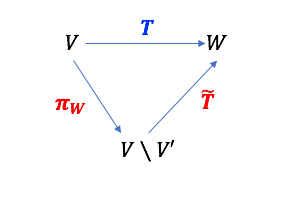
\includegraphics[width=0.5\textwidth]{week4/p_1}
\end{figure}
In other words, we have $T = \tilde{T}\circ \pi_W$.
\end{proposition}

\begin{proof}
First we show the well-definedness. Suppose that $\bm v_1+V'=\bm v_2+V'$ and suffices to show $\tilde T(\bm v_1+V')=\tilde T(\bm v_2+V')$, i.e., $T(\bm v_1)=T(\bm v_2)$. By proposition~(\ref{pro:4:1}), we imply
\[
\bm v_1-\bm v_2\in V'\le\ker(T)\implies
T(\bm v_1-\bm v_2)=\bm0\implies T(\bm v_1)-T(\bm v_2)=\bm0.
\]
Then we show $\tilde(T)$ is a linear transformation:
\begin{align*}
\tilde{T}(\alpha(\bm v_1+V')  + \beta(\bm v_2+V'))&=\tilde{T}((\alpha\bm v_1+\beta\bm v_2)+V')\\
&=T(\alpha\bm v_1+\beta\bm v_2)\\
&=\alpha T(\bm v_1)+\beta T(\bm v_2)\\
&=\alpha\tilde{T}(\bm v_1+V')+\beta\tilde{T}(\bm v_2+V')
\end{align*}
\end{proof}

Actually, if we let $V'=\ker(T)$, the mapping $\tilde{T}:V/ V'\to T(V)$ forms an isomorphism, In particular, if further $T$ is surjective, then $T(V)=W$, i.e., the mapping $\tilde{T}:V/ V'\to W$ forms an isomorphism.
\begin{theorem}[First Isomorphism Theorem]
Let $T:V\to W$ be a surjective linear transformation. Then the mapping 
\begin{align*}
\tilde{T}&:V/ \ker(T)\to W\\
&\bm v+\ker(T)\mapsto T(\bm v)
\end{align*}
is an isomorphism.
\end{theorem}
\begin{proof}
\textit{Injectivity.} Suppose that $\tilde{T}(\bm v_1+\ker(T)) = \tilde{T}(\bm v_2+\ker(T))$, then we imply
\[
T(\bm v_1)=T(\bm v_2)\implies T(\bm v_1-\bm v_2)=\bm0_W\implies\bm v_1-\bm v_2\in\ker(T),
\]
i.e., $\bm v_1+\ker(T)=\bm v_2+\ker(T)$.

\textit{Surjectivity.} For $\bm w\in W$, due to the surjectivity of $T$, we can find a $\bm v_0$ such that $T(\bm v_0)=\bm w$. Therefore, we can construct a set $\bm v_0+\ker(T)$ such that
\[
\tilde{T}(\bm v_0+\ker(T))=\bm w.
\]
\end{proof}




















\section{Monday for MAT3006}\index{Monday_lecture}
\subsection{Remarks on MCT}
\begin{example}
The MCT can help us to compute the integral
\begin{align*}
\lim_{n\to\infty}\int_{[0,n\pi]}\cos\left(\frac{x}{2n}\right)xe^{-x^2}\diff x
\end{align*}

Construct $f_n(x) = \cos\left(\frac{x}{2n}\right)xe^{-x^2}\mathcal{X}_{[0,n\pi]}$.
\begin{itemize}
\item
Since $\cos(x/2n)<\cos(x/2(n+1))$ for any $x\in[0,n\pi]$, we imply $f_n$ is monotone increasing with $n$
\item
$f_n(x)$ is integrable for all $n$.
\item
$f_n$ converges pointwise to $xe^{-x^2}\mathcal{X}_{[0,\infty)}$
\end{itemize}
Therefore, MCT I applies and
\[
\lim_{n\to\infty}\int_{[0,n\pi]}\cos\left(\frac{x}{2n}\right)xe^{-x^2}\diff x
=
\int\left(\lim_{n\to\infty}f_n\right)\diff m
\]
with
\[
\lim_{n\to\infty}f_n = xe^{-x^2}\mathcal{X}_{[0,\infty)}.
\]
Moreover, 
\begin{subequations}
\begin{align}
\int\left(\lim_{n\to\infty}f_n\right)\diff m &= 
\lim_{m\to\infty}\int_{[0,m]}xe^{-x^2}\diff x\label{Eq:12:1}\\
&=\int_0^\infty xe^{-x^2}\diff x\\
&=\frac{1}{2}
\end{align}
where (\ref{Eq:12:1}) is by applying MCT I with $g_m(x) = xe^{-x^2}\mathcal{X}_{[0,m]}$ and proposition~(\ref{pro:10:14}) to compute a Lebesgue integral by evaluating a proper Riemann integral.
\end{subequations}
\end{example}

Then we discuss the Lebesgue integral for series:

\begin{corollary}[Lebesgue Series Theorem]
Let $\{f_n\}$ be a series of measurable functions such that
\[
\sum_{n=1}^\infty\int|f_n|\diff m<\infty,
\]
then $\sum_{n=1}^kf_n$ converges to an integrable function $f = \sum_{n=1}^\infty f_n$ a.e., with
\[
\int f\diff m = \sum_{n=1}^\infty\int f_n\diff m
\]
\end{corollary}
\begin{proof}
\begin{itemize}
\item
For each $f_n$, consider 
\[
f_n = f_n^+ - f_n^-,\ \text{where $f_n^+,f_n^-$ are nonnegative}.
\]
By proposition~(\ref{pro:11:6}), 
\[
\int\sum_{n=1}^\infty f_n^+\diff m = \sum_{n=1}^\infty\int f_n^+\diff m\le \sum_{n=1}^\infty\int |f_n|\diff m<\infty.
\]
Therefore, $f^+:=\sum_{n=1}^\infty f_n^+=\lim_{k\to\infty}\sum_{n=1}^kf_n^+$ is integrable.
The same follows by replacing $f^{+}$ with $f^{-}$.
By corollary~(\ref{cor:9:6}), $f^+(x),f^-(x)<\infty,\forall x\in U$, where $U^c$ is null.
\item
Therefore, construct 
\[
f(x)=\left\{
\begin{aligned}
f^+(x)-f^-(x),&\quad x\in U\\
0,&\quad x\in U^c
\end{aligned}
\right.
\]
Moreover, for $x\in U$, 
\begin{align*}
f(x)&=\left(\lim_{k\to\infty}\sum_{n=1}^kf_n^+(x)\right)-
\left(\lim_{k\to\infty}\sum_{n=1}^kf_n^-(x)\right)\\
&=\lim_{k\to\infty}
\left(
\sum_{n=1}^kf_n^+(x)
-
\sum_{n=1}^kf_n^-(x)
\right)\\
&=\lim_{k\to\infty}\left[\sum_{n=1}^k(f_n^+(x)-f_n^-(x))\right]
\\&=
\sum_{n=1}^\infty f_n(x)
\end{align*}
where the first equality is because that both terms are finite.
\item
It follows that
\begin{subequations}
\begin{align}
\int f\diff m&=\int f^+\diff m - \int f^-\diff m\label{Eq:12:2:a}\\
&=
\int\sum_{n=1}^\infty f_n^+\diff m -\int\sum_{n=1}^\infty f_n^-\diff m\\
&=\left(\sum_{n=1}^\infty\int f_n^+\diff m\right)
-
\left(\sum_{n=1}^\infty\int f_n^-\diff m\right)\label{Eq:12:2:c}\\
&=\sum_{n=1}^\infty
\left(
\int f_n^+\diff m -\int f_n^-\diff m
\right)\label{Eq:12:2:d}\\
&=\sum_{n=1}^\infty\int f_n\diff m\label{Eq:12:2:e}
\end{align}
where (\ref{Eq:12:2:a}),(\ref{Eq:12:2:d}) is because that summation/subtraction between series holds when these series are finite; (\ref{Eq:12:2:c}) is by proposition~(\ref{pro:11:6}); (\ref{Eq:12:2:e}) is by definition of $f_n$.
\end{subequations}
\end{itemize}
\end{proof}

\begin{example}
Compute the integral
\[
\int_{(0,1]}e^{-x}x^{\alpha-1}\diff x,\ \alpha>0.
\]
\begin{itemize}
\item
Construct $f_n(x) = (-1)^n\frac{x^{\alpha+n-1}}{n!}\mathcal{X}_{(0,1]}, n\ge0$, and
\[
\sum_{n=0}^N f_n(x)\to e^{-x}x^{\alpha-1}, \ \text{pointwisely}, x\in(0,1]. 
\]
By applying MCT I,
\[
\int|f_n|\diff m=\frac{1}{(\alpha+n)n!}
\]
Therefore, 
\[
\sum_{n=0}^\infty\int|f_n|\diff m=
\sum_{n=0}^\infty\frac{1}{(\alpha+n)n!}<\infty
\]
\item
Applying the Lebesgue Series Theorem,
\[
\int_{(0,1]}e^{-x}x^{\alpha-1}\diff x = 
\int_{(0,1]}(\sum_{n=0}^\infty f_n)\diff m
=
\sum_{n=0}^\infty\int f_n\diff m=
\sum_{n=0}^\infty\frac{(-1)^n}{(\alpha+n)n!}
\]
\end{itemize}
\end{example}

\begin{remark}
It's essential to have $\sum\int|f|\diff m<\infty$ rather than $\sum\int f_n\diff m<\infty$ in the Lebesgue Series Theorem.
For example, let
\[
f_n=\frac{(-1)^{n+1}}{(n+1)}\mathcal{X}_{[n,n+1)}
\implies
\sum_{n=1}^\infty\int f_n\diff m =\log(2)<\infty
\]
However, $f:=\sum f_n$ is not integrable.
\end{remark}

\subsection{Dominated Convergence Theorem}
\begin{theorem}
Let $\{f_n\}$ be a sequence of measruable functions such that $|f_n|\le g$ a.e., and $g$ is integrable.
Suppose that $\lim_{n\to\infty}f_n(x)=f(x)$ a.e., then
\begin{enumerate}
\item
$f$ is integrable,
\item
\[
\int f\diff m =\lim_{n\to\infty}\int f_n\diff m
\]
\end{enumerate}
\end{theorem}
\begin{proof}
\begin{itemize}
\item
Observe that 
\[
|f_n|\le g\implies
\lim_{n\to\infty}|f_n|\le g\implies |f|\le g
\]
By comparison test, $g$ is integrable implies $|f|$ is integrable, and further $f$ is integrable.
\item
Consider the sequence of non-negative functions
$\{g-f_n\}_{n\in\mathbb{N}}$ and $\{g+f_n\}_{n\in\mathbb{N}}$.

By Fatou's Lemma, 
\begin{align*}
\lim_{n\to\infty}\inf\int(g-f_n)\diff m&\ge \int \lim_{n\to\infty}\inf(g-f_n)\diff m\\
&=\int(g-f)\diff m\\
&=\int g\diff m - \int f\diff m
\end{align*}
which follows that
\[
\int g\diff m - \lim_{n\to\infty}\sup\int f_n\diff m
\ge
\int g\diff m - \int f\diff m
\]
i.e.,
\[
\int f\diff m\ge  \lim_{n\to\infty}\sup\int f_n\diff m
\]
\item
Similarly, 
\[
\lim_{n\to\infty}\inf(g+f_n)\diff m\ge \int\lim_{n\to\infty}\inf(g+f_n)\diff m
=
\int g\diff m + \int f\diff m
\]
which implies
\[
 \lim_{n\to\infty}\inf\int f_n\diff m\ge\int f\diff m
\]
\end{itemize}
As a result,
\[
 \lim_{n\to\infty}\sup\int f_n\diff m
 \le
 \int f\diff m\le  \lim_{n\to\infty}\inf\int f_n\diff m,
\]
which implies
\[
\int f\diff m = \lim_n\int f_n\diff m
\]
\end{proof}

\begin{corollary}[Bounded Convergence Theorem]
Suppose that $E\in\mathcal{M}$ be such that $m(E)<\infty$.
If
\begin{itemize}
\item
$|f_n(x)|\le K<\infty$ for any $x\in E,n\in\mathbb{N}$
\item
$f_n\to f$ a.e. in $E$,
\end{itemize}
then $f$ is integrable in $E$ with
\[
\int_Ef\diff m = \lim_{n\to\infty}\int f_n\diff m
\]
\end{corollary}
\begin{proof}
Take $g=K\mathcal{X}_E$ in DCT.
\end{proof}


\begin{proposition}
Every Riemann integrable function $f$ on $[a,b]$ is Lebesgue integrable, without the condition that $f$ is continuous a.e.
\end{proposition}
\begin{proof}
Since $f$ is Riemann integrable, we imply $f$ is bounded.
We construct the Riemann lower abd upper functions with $2^n$ equal intervals, denoted as $\{\phi_n\}$ and $\{\psi_n\}$, which follows that
\begin{itemize}
\item
$\phi_n$ is monotone increasing;
$\psi_n$ is monotone decreasing;
\item
$\phi_n\le f\le \psi_n$, and
\[
\lim_{n\to\infty}\int_{[a,b]}\phi_n=\int_a^bf(x)\diff x = \lim_{n\to\infty}\int_{[a,b]}\psi_n.
\]
\end{itemize}
Construct $g=\sup_n\phi_n$ and $h=\inf_n\psi_n$.
Now we can apply the bounded convergence theorem:
\begin{itemize}
\item
$\phi_n$ is bounded on $[a,b]$
\item
$\phi_n\to g$ on $[a,b]$
\end{itemize}
which implies
$g$ is Lebesgue integrable on $[a,b]$, with 
\[
\int_{[a,b]}g\diff m = \lim_{n\to\infty}\int_{[a,b]}\phi_n\diff m=\int_a^bf(x)\diff x.
\]
Similarly, $h$ is Lebesgue integrable, with
\[
\int_{[a,b]}h\diff m = \lim_{n\to\infty}\int_{[a,b]}\psi_n\diff m=\int_a^bf(x)\diff x.
\]
Moreover, $g\le f\le h$, and
\[
\int_{[a,b]}(h-g)\diff m = \int_{[a,b]}h\diff m - \int_{[a,b]}g\diff m=\int_a^bf(x)\diff x-\int_a^bf(x)\diff x=0,
\]
which implies $h=g$ a.e., and further $f=g$ a.e., which implies
\[
\int_{[a,b]} f\diff m = \int_{[a,b]} g\diff m= \int_a^bf(x)\diff x.
\]
\end{proof}
\begin{remark}
However, an improper Riemann integral does not necessarily has the corresponding Lebesgue integral:
\[
f(x)=\sum_{n=1}^\infty (-1)^nn\cdot\mathcal{X}_{(1/(n+1),1/n]},\ x\in[0,1]
\]
In this case, $f$ is Riemann integrable but not Lebesgue integrable.
\end{remark}














\section{Monday for MAT4002}\index{Monday_lecture}

\paragraph{Reviewing}
\begin{enumerate}
\item
Topological Space $(X,\mathcal{J})$: a special class of topological space is that induced from metric space $(X,d)$:
\[
(X,\mathcal{T}),\quad\text{with }\mathcal{T}=\{\text{all open sets in $(X,d)$}\}
\]
\item
Closed Sets $(X\setminus U)$ with $U$ open.
\end{enumerate}

\begin{proposition}
Let $(X,\mathcal{T})$ be a topological space, 
\begin{enumerate}
\item
$\emptyset, X$ are closed in $X$
\item
$V_1,V_2$ closed in $X$ implies that $V_1\bigcup V_2$ closed in $X$
\item
$\{V_\alpha\mid\alpha\in\mathcal{A}\}$ closed in $X$ implies that $\bigcap_{\alpha\in\mathcal{A}}V_\alpha$ closed in $X$
\end{enumerate}
\end{proposition}
\begin{proof}
Applying the De Morgan's Law
\[
(X\setminus\bigcup_{i\in I}U_i)=\bigcap_{i\in I}(X\setminus U_i)
\]
\end{proof}

\subsection{Convergence in topological space}

\begin{definition}[Convergence]
A sequence $\{x_n\}$ of a topological space $(X,\mathcal{T})$ converges to $x\in X$ 
if $\forall U\ni x$ is open, there $\exists N$ such that $x_n\in U,\forall n\ge N$.
\end{definition}

\begin{example}
\begin{enumerate}
\item
The topology for the space $(X=\mathbb{R}^n,d_2)\to(X,\mathcal{T})$ (i.e., a topological space induced from meric space $(X=\mathbb{R}^n,d_2)$) is called a \emph{usual topology} on $\mathbb{R}^n$.

When I say $\mathbb{R}^n$ (or subset of $\mathbb{R}^n$) is a topological space, 
it is equipeed with usual topology.

Convergence of sequence in $(\mathbb{R}^n,\mathcal{T})$ is the usual convergence in analysis.

For $\mathbb{R}^n$ or metric space, the limit of sequence (if exists) is unique.

\item

Consider the topological space $(X,\mathcal{T}_{\text{indiscrete}})$. 
Take any sequence $\{x_n\}$ in $X$, it is convergent to any $x\in X$. 
Indeed, for $\forall U\ni x$ open, $U=X$. Therefore, 
\[
x_n\in U(=X),\forall n\ge1.
\]
\item

Consider the topological space $(X,\mathcal{T}_{\text{cofinite}})$, where $X$ is infinite. 
Consider $\{x_n\}$ is a sequence satisfying $m\ne n$ implies $x_m\ne x_n$. 
Then $\{x_n\}$ is convergent to any $x\in X$.

(Question: how to define openness for $\mathcal{T}_{\text{cofinite}}$ and $\mathcal{T}_{\text{indiscrete}})$?
\item

Consider the topological space $(X,\mathcal{T}_{\text{discrete}})$, 
the sequence $\{x_n\}\to x$ is equivalent to say $x_n=x$ for all sufficiently large $n$.
\end{enumerate}
\end{example}
\begin{remark}
The limit of sequences may not be unique. The reason is that ``$\mathcal{T}$ is not big enough''. We will give a criterion to make sure the limit is unique in the future. (Hausdorff)
\end{remark}
\begin{proposition}\label{pro:2:9}
If $F\subseteq(X,\mathcal{T})$ is closed, then for any convergent sequence $\{x_n\}$ in $F$, the limit(s) are also in $F$.
\end{proposition}

\begin{proof}
Let $\{x_n\}$ be a sequence in $F$ with limit $x\in X$. 
Suppose on the contrary that $x\notin F$ 
(i.e., $x\in X\setminus F$ that is open). 
There exists $N$ such that
\[
x_n\in X\setminus F,\forall n\ge N,
\]
i.e., $x_n\notin F$, which is a contradiction.
\end{proof}
\begin{remark}
The converse may not be true. If the $(X,\mathcal{T})$ is metrizable, the converse holds.

Counter-example: Consider the co-countable topological space $(X=\mathbb{R},\mathcal{T}_{\text{co-co}})$, where 
\[
\mathcal{T}_{\text{co-co}}=
\{U\mid X\setminus U\text{ is a countable set}\}
\bigcup\{\emptyset\},
\]
and $X$ is uncontable. 
Then note that $F=[0,1]\subsetneqq X$ is an un-countable set, and under co-countable topology, $F\supseteq \{x_n\}\to x$ implies $x_n=x\in F$ for all $n$.
It's clear that $X\setminus F\notin \mathcal{T}_{\text{co-co}}$, i.e., $F$ is not closed.
\end{remark}

\subsection{Interior, Closure, Boundary}
\begin{definition}\label{def:2:5}
Let $(X,\mathcal{T})$ be a topological space, and $A\subseteq X$ a subset.
\begin{enumerate}
\item
The \emph{interior} of $A$ is 
\[
A^\circ=\bigcup_{U\subseteq A,U\text{ is open}}U
\]
\item
The \emph{closure} of $A$ is
\[
\overline{A}=\bigcap_{A\subseteq V,V\text{ is closed}}V
\]
\end{enumerate}

If $\overline{A}=X$, we say that $A$ is dense in $X$.

The graph illustration of the definition above is as follows:
\begin{figure}[H]
        \begin{subfigure}[b]{0.3\textwidth}
                \centering
                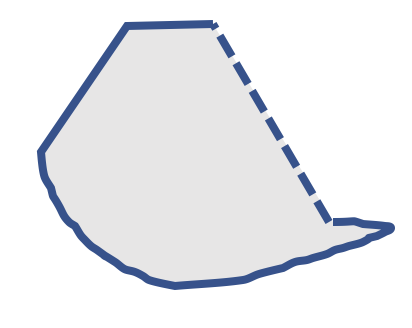
\includegraphics[width=\textwidth]{week2/p_1}
                \caption{Illustration of $A$}
                \label{fig:gull}
        \end{subfigure}%
        \begin{subfigure}[b]{0.3\textwidth}
                \centering
                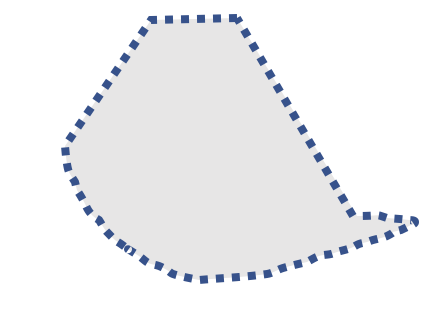
\includegraphics[width=\textwidth]{week2/p_2}
                \caption{Illustration of $A^\circ$}
                \label{fig:gull2}
        \end{subfigure}%
        \begin{subfigure}[b]{0.3\textwidth}
                \centering
                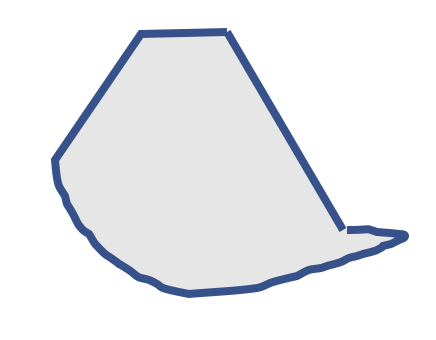
\includegraphics[width=\textwidth]{week2/p_3}
                \caption{Illustration of $\overline{A}$}
                \label{fig:tiger}
        \end{subfigure}
        \caption{Graph Illustrations}\label{fig:animals}
\end{figure}
\end{definition}
\begin{example}
\begin{enumerate}
\item

For $[a,b)\subseteq\mathbb{R}$, we have:
\[
\begin{array}{ll}
[a,b)^\circ=(a,b),
&
\overline{[a,b)}=[a,b]
\end{array}
\]

\item
For $X=\mathbb{R}$, $\mathbb{Q}^\circ=\emptyset$ and $\overline{\mathbb{Q}}=\mathbb{R}$.

\item
Consider the discrete topology $(X,\mathcal{T}_{\text{discrete}})$, we have
\[
\begin{array}{ll}
S^\circ=S,
&
\overline{S}=S
\end{array}
\]

\end{enumerate}
\end{example}

The insights behind the definition~(\ref{def:2:5}) is as follows

\begin{proposition}
\begin{enumerate}
\item
$A^\circ$ is the largest open subset of $X$ contained in $A$;

$\overline{A}$ is the smallest closed subset of $X$ containing $A$.
\item
If $A\subseteq B$, then $A^\circ\subseteq B$ and $\overline{A}\subseteq\overline{B}$
\item
$A$ is open in $X$ is equivalent to say $A^\circ = A$; $A$ is closed in $X$ is equivalent to say $\overline{A}=A$.
\end{enumerate}
\end{proposition}

\begin{example}
Let $(X,d)$ be a metric space. What's the closure of an open ball $B_r(x)$?

The direct intuition is to define the closed ball
\[
\bar B_r(x)=\{y\in X\mid d(x,y)\le r\}.
\]

Question: is $\bar B_r(x)=\overline{B_r(x)}$?
\begin{enumerate}
\item
Since $\bar B_r(x)$ is a closed subset of $X$, and 
$B_r(x)\subseteq \bar B_r(x)$, 
we imply that
\[
\overline{B_r(x)}\subseteq\bar B_r(x)
\]
\item
Howover, we may find an example such that $\overline{B_r(x)}$ is a proper subset of $\bar B_r(x)$:

Consider the discrete metric space $(X,d_{\text{discrete}})$ and for $\forall x\in X$,
\[
B_1(x)=\{x\}\implies
\overline{B_1(x)}=\{x\},\quad
\bar B_1(x)=X
\]

The equality $\bar B_r(x)=\overline{B_r(x)}$ holds when $(X,d)$ is a normed space.
\end{enumerate}
\end{example}

Here is another characterization of $\overline{A}$:

\begin{proposition}\label{pro:2:11}
\[
\overline{A}=\{x\in X\mid\forall \text{open }U\ni x, U\bigcap A\ne\emptyset\}
\]
\end{proposition}
\begin{proof}
Define
\[
S=\{x\in X\mid\forall \text{open }U\ni x, U\bigcap A\ne\emptyset\}
\]
It suffices to show that $\overline{A}=S$.
\begin{enumerate}
\item
First show that $S$ is closed:
\[
X\setminus S=\{x\in X\mid\exists U_x\ni x\text{ open s.t. }U_x\bigcap A=\emptyset\}
\]
Take $x\in X\setminus S$, we imply there exists open $U_x\ni x$ such that $U_x\bigcap A=\emptyset$. We claim $U_x\subseteq X\setminus S$:
\begin{itemize}
\item
For $\forall y\in U_x$, note that $U_x\ni y$ that is open, such that $U_x\bigcap A=\emptyset$. Therefore, $y\in X\setminus S$.
\end{itemize}

Therefore, we have $x\in U_x\subseteq X\setminus S$ for any $\forall x\in X\setminus S$.

Note that
\[
X\setminus S
=
\bigcup_{x\in X\setminus S}\{x\}\subseteq
\bigcup_{x\in X\setminus S}U_x\subseteq X\setminus S,
\]
which implies $X\setminus S=\bigcup_{x\in X\setminus S}U_x$ is open, i.e., $S$ is closed in $X$.
\item
By definition, it is clear that $A\subseteq S$:
\[
\forall a\in A,\forall\text{open }U\ni a,
U\bigcap A\supseteq\{a\}\ne\emptyset\implies a\in S.
\]
Therefore, $\overline{A}\subseteq\overline{S}=S$.
\item
Suppose on the contrary that 
there exists $y\in S\setminus\overline{A}$. 

Since $y\notin\overline{A}$, by definition, 
there exists $F\supseteq A$ closed such that 
$y\notin F$. 

Therefore, $y\in X\setminus F$ that is open, and 
\[
(X\setminus F)\bigcap A\subseteq(X\setminus A)\bigcap A=\emptyset\implies y\notin S,
\]
which is a contradiction. Therefore, $S=\overline{A}$.
\end{enumerate}
\end{proof}
\begin{definition}[accumulation point]
Let $A\subseteq X$ be a subset in a topological space. 
We call $x\in X$ are an 
\emph{accumulation point} (\emph{limit point}) of $A$ 
if
\[
\forall U\subseteq X\text{ open s.t. }
U\ni x, 
(U\setminus\{x\})\bigcap A\ne\emptyset.
\]

The set of accumulation points of $A$ is denoted as $A'$
\end{definition}
\begin{proposition}
$\overline{A}=A\bigcup A'$.
\end{proposition}

\begin{proof}
This proposition directly follows from Proposition~(\ref{pro:2:11}) and the definition of A'.
\end{proof}













\section{Wednesday for MAT3040}\index{Wednesday_lecture}
\subsection{Tensor Product for Linear Transformations}

\begin{proposition}
Suppose that $T:V\to V'$ and $S:W\to W'$ are linear transformations, then there exists an unique linear transformation 
\[
\begin{array}{ll}
T\otimes S:&V\otimes W\to V'\otimes W'\\
\text{satisfying}&(T\otimes S)(v\otimes w) = T(v)\otimes S(w)
\end{array}
\]
\end{proposition}

\begin{proof}
We construct the mapping
\[
\begin{array}{ll}
T\times S:&V\times W\to V'\otimes W'\\
\text{with}&(T\times S)(v,w) = T(v)\otimes S(w)
\end{array}
\]
This mapping is indeed bilinear: for instance, we can show that 
\[
(T\times S)(av_1+bv_2,w) = a(T\times S)(v_1,w)+b(T\times S)(v_2,w)
\]
Therefore, $T\times S\in\text{Obj}$. Since the tensor product satisfies the universal property, we imply there exists an unique linear transformation
\[
\begin{array}{ll}
T\otimes S&V\otimes W\to V'\otimes W'\\
\text{satisfying}&(T\otimes S)(v\otimes w)=T(v)\otimes S(w)
\end{array}
\]


\end{proof}
\paragraph{Notation Warning}
Does the notion $T\otimes S$ really form a tensor product, i.e., do we obtain the addictive rules for tensor product such as 
\[
(aT_1+bT_2)\otimes S = a(T_1\otimes S)+b(T_2\otimes S)?
\]


\begin{example}\label{exp:13:2}
Let $V=V'=\mathbb{F}^2$ and $W=W'=\mathbb{F}^3$.
Define the matrix-multiply mappings:
\[\left\{
\begin{array}{ll}
T:&V\to V\\
\text{with}&\bm v\mapsto\bm A\bm v\\
&\bm A=\begin{pmatrix}
a&b\\c&d
\end{pmatrix}
\end{array}\right.\qquad
\left\{
\begin{array}{ll}
S:&W\to W\\
\text{with}&\bm w\mapsto\bm B\bm w\\
&\bm B=\begin{pmatrix}
p&q&r\\
s&t&u\\
v&w&x
\end{pmatrix}
\end{array}
\right.
\]
How does $T\otimes S:V\otimes W\to V\otimes W$ look like?
\begin{itemize}
\item
Suppose $\{e_1,e_2\},\{f_1,f_2,f_3\}$ are usual basis of $V,W$, respectively.
Then the basis of $V\otimes W$ is given by:
\[
\mathcal{C}=\{e_1\otimes f_1,e_1\otimes f_2,e_1\otimes f_3,e_2\otimes f_1,e_2\otimes f_2,e_2\otimes f_3\}.
\]
\item
As a result, we can compute $(T\otimes S)(e_i\otimes f_j)$ for $i=1,2$ and $j=1,2,3$. For instance,
\begin{align*}
(T\otimes S)(e_1\otimes e_1)&=T(e_1)\otimes S(e_1)\\
&=(ae_1+ce_2)\otimes(pe_1+se_2+ve_3)\\
&=
(ap)e_1\otimes e_1+(as)e_1\otimes e_2+(av)e_1\otimes e_3+(cp)e_2\otimes e_1+(cs)e_2\otimes e_2+(cv)e_2\otimes e_3
\end{align*}
\item
Therefore, we obtain a matrix representation for the linear transformation $(T\otimes S)$:

\end{itemize}
We want a matrix representation for $(T\otimes S)$:
\[
(T\otimes S)_{\mathcal{C},\mathcal{C}}
=
\begin{pmatrix}
aB&bB\\
cB&dB
\end{pmatrix},
\]
which is a large matrix formed by taking all possible products between the elements of $\bm A$ and those of $\bm B$.
This operation is called the \emph{Kronecker Tensor Product}, see the command \textit{kron} in MATLAB for detail.


\end{example}
\begin{proposition}
More generally, given the linear operator $T:V\to V$ and $S:W\to W$, 
let $\mathcal{A}=\{v_1,\dots,v_n\},\mathcal{B}=\{w_1,\dots,w_m\}$ be a basis of $V,W$ respectively, with
\[
\begin{array}{ll}
(T)_{\mathcal{A},\mathcal{A}}=(a_{ij})
&
(S_{\mathcal{B},\mathcal{B}})=(b_{ij}):=B
\end{array}
\]
As a result, $(T\otimes S)_{\mathcal{C},\mathcal{C}}=A\otimes B$, where 
$\mathcal{C}=\{v_1\otimes w_1,\dots, v_n\otimes w_m\}$, and $A\otimes B$ denotes the Kronecker tensor product, defined as the matrix
\[
\begin{pmatrix}
a_{1,1}B&\cdots&a_{1,n}B\\
\vdots&\ddots&\vdots\\
a_{n,1}B&\cdots&a_{n,n}B
\end{pmatrix}.
\]
\end{proposition}
\begin{proof}
Following the similar procedure as in Example~(\ref{exp:13:2}) and applying the relation
\begin{align*}
(T\otimes S)(v_i\otimes w_j)&=T(v_i)\otimes S(w_j)\\
&=\left(
\sum_{k=1}^na_{ki}v_k
\right)
\otimes
\left(
\sum_{\ell=1}^mb_{\ell j}w_\ell
\right)\\
&=\sum_{k=1}^n\sum_{\ell=1}^m(a_{ki}b_{\ell j})v_k\otimes w_{\ell}
\end{align*}
\end{proof}

\begin{proposition}
The operation $T\otimes S$ satisfies all the properties of tensor product.
For example,
\begin{align*}
(aT_1+bT_2)\otimes S &= a(T_1\otimes S)+b(T_2\otimes S)\\
T\otimes(cS_1+dS_2) &= c(T\otimes S_1)+d(T\otimes S_2)
\end{align*}
Therefore, the usage of the notion ``$\otimes$'' is justified for the definition of $T\otimes S$.
\end{proposition}
\begin{proof}[Proof using matrix multiplication]
For instance, consider the operation $(T+T')\otimes S$, with $(T)_{\mathcal{A},\mathcal{A}}=(a_{ij})$, $(T')_{\mathcal{A},\mathcal{A}}=(c_{ij}), (S)_{\mathcal{B},\mathcal{B}}=B$.

We compute its matrix representation directly:
\begin{align*}
((T+T')\otimes S)_{\mathcal{C},\mathcal{C}}
&=
(T+T')_{\mathcal{A},\mathcal{A}}\otimes (S)_{\mathcal{B},\mathcal{B}}\\
&=
[(T)_{\mathcal{A},\mathcal{A}}+(T')_{\mathcal{A},\mathcal{A}}]\otimes (S)_{\mathcal{B},\mathcal{B}}\\
&=
(T)_{\mathcal{A},\mathcal{A}}\otimes (S)_{\mathcal{B},\mathcal{B}}
+
(T')_{\mathcal{A},\mathcal{A}}\otimes (S)_{\mathcal{B},\mathcal{B}}
\end{align*}
where the last equality is by the addictive rule for kronecker product for matrices.
Therefore,
\[
((T+T')\otimes S)_{\mathcal{C},\mathcal{C}}=
(T\otimes S)_{\mathcal{C},\mathcal{C}} + 
(T'\otimes S)_{\mathcal{C},\mathcal{C}}
\implies
(T+T')\otimes S
=
T\otimes S+T'\otimes S
\]
\end{proof}
\begin{proof}[Proof using basis of $T\otimes S$]
Another way of the proof is by computing 
\[
((T+T')\otimes S)(v_i\otimes w_j),
\] 
where $\{v_i\otimes w_j\mid 1\le i\le n,1\le j\le m\}$ forms a basis of $(T+T')\otimes S$:
\begin{align*}
((T+T')\otimes S)(v_i\otimes w_j)
&=(T+T')(v_i)\otimes S(w_j)\\
&=(T(v_i)+T'(v_i))\otimes S(w_j)\\
&=T(v_i)\otimes S(w_j)+T'(v_i)\otimes S(w_j)\\
&=(T\otimes S)(v_i\otimes w_j)+(T'\otimes S)(v_i\otimes w_j)
\end{align*}
Since $((T+T')\otimes S)(v_i\otimes w_j)$ coincides with $(T\otimes S + T'\otimes S)(v_i\otimes w_j)$ for all basis vectors $v_i\otimes w_j\in\mathcal{C}$, we imply
\[
(T+T')\otimes S = T\otimes S+T'\otimes S
\]
\end{proof}


\begin{proposition}
Let $A,C$ be linear operators from $V$ to $V$, and $B,D$ be linear operators from $W$ to $W$, then
\[
(A\otimes B)\circ(C\otimes D)=(AC)\otimes(BD)
\]
\end{proposition}

\begin{proposition}
Define linear operators $A:V\to V$ and $B:W\to W$ with $\dim(V),\dim(W)<\infty$.
Then
\[
\det(A\otimes B) = (\det(A))^{\dim(W)}(\det(B))^{\dim(V)}
\]
\end{proposition}

\begin{corollary}
There exists a linear transformation 
\[
\begin{array}{ll}
\Phi:&
\text{Hom}(V,V)\otimes\text{Hom}(W,W)\to
\text{Hom}(V\otimes W,V\otimes W)\\
\text{with}&A\otimes B\mapsto A\otimes B
\end{array}
\]
where the input of $\Phi$ is the tensor product of linear transformations, and the output is the linear transformation.
\end{corollary}
\begin{proof}
Construct the mapping
\[
\begin{array}{ll}
\Phi&:
\text{Hom}(V,V)\times\text{Hom}(W,W)\to
\text{Hom}(V\otimes W,V\otimes W)\\
\text{with}&\Phi(A,B)=A\otimes B
\end{array}
\]
The $\Phi$ is indeed bilinear: for instance, 
\begin{align*}
\Phi(pA+qC,B)&=(pA+qC)\otimes B\\
&=p(A\otimes B)+q(C\otimes B)\\
&=p\Phi(A,B)+q\Phi(C,B)
\end{align*}
This corollary follows from the universal property of tensor product.
\end{proof}
\begin{remark}
If assuming that $\dim(V),\dim(W)<\infty$, we imply
\begin{align*}
\dim(\text{Input space of $\Phi$})&=\dim(\text{Hom}(V,V))\dim(\text{Hom}(W,W))\\
&=
[\dim(V)\dim(V)]
\cdot
[\dim(W)\dim(W)]
=
[\dim(V)\dim(W)]^2\\
&=[\dim(V\otimes W)]^2\\
&=\dim(\text{Hom}(V\otimes W,V\otimes W))\\
&=\dim(\text{Output space of $\Phi$})
\end{align*}
Therefore, is $\Phi$ is an isomorphism?
If so, then every linear operator $\alpha:V\otimes W\to V\otimes W$ can be expressed as
\[
\alpha = A_1\otimes B_1+\cdots+A_k\otimes B_k
\]
where $A_i:V\to V$ and $B_j:W\to W$.
\end{remark}











\section{Wednesday for MAT3006}\index{Monday_lecture}
\paragraph{Reviewing}
\begin{itemize}
\item
Normed Space: a norm on a vector space
\item
Metric Space
\item
Open Ball
\end{itemize}
\subsection{Convergence of Sequences}
Since $\mathbb{R}^n$ and $\mathcal{C}[a,b]$ are both metric spaces, we can study the convergence in $\mathbb{R}^n$ and the functions defined on $[a,b]$ at the same time.

\begin{definition}[Convergence]
Let $(X,d)$ be a metric space. 
A sequence $\{x_n\}$ in $X$ is \emph{convergent} to $x$
if $\forall\varepsilon>0$, there exists $N\in\mathbb{N}$ such that
\[
d(x_n,x)<\varepsilon,\forall n\ge N.
\]
We can denote the convergence by
\[
\begin{array}{lllll}
x_n\to x,
&
\mbox{or}
&
\displaystyle
\lim_{n\to\infty}x_n=x,
&
\mbox{or}
&\displaystyle
\lim_{n\to\infty}d(x_n,x)=0
\end{array}
\]
\end{definition}
\begin{proposition}
If the limit of $\{x_n\}$ exists, then it is unique.
\end{proposition}
\begin{remark}
Note that the proposition above does not necessarily hold for topology spaces.
\end{remark}
\begin{proof}
Suppose $x_n\to x$ and $x_n\to y$, which implies
\[
0\le d(x,y)\le d(x,x_n)+d(x_n,y),\forall n
\]
Taking the limit $n\to\infty$ both sides, we imply $d(x,y)=0$, i.e., $x=y$.
\end{proof}
\begin{example}\label{Exp:1:16}
\begin{enumerate}
\item
Consider the metric space $(\mathbb{R}^k,d_\infty)$ and study the convergence
\begin{align*}
\lim_{n\to\infty}\bm x_n=\bm x&\Longleftrightarrow
\lim_{n\to\infty}\left(\max_{i=1\dots,k}|x_{n_i}-x_i|\right)=0\\
&\Longleftrightarrow
\lim_{n\to\infty}|x_{n_i}-x_i|=0,\forall i=1,\dots,k\\
&\Longleftrightarrow
\lim_{n\to\infty}x_{n_i}=x_i,
\end{align*}
i.e., the convergence defined in $d_\infty$ is the same as the convergence defined in $d_2$.
\item
Consider the convergence in the metric space $(\mathcal{C}[a,b],d_\infty)$:
\begin{align*}
\lim_{n\to\infty}f_n=f&\Longleftrightarrow
\lim_{n\to\infty}\left(\max_{[a,b]}|f_n(x)-f(x)|\right)=0\\
&\Longleftrightarrow
\forall\varepsilon>0,\forall x\in[a,b],\exists N_{\varepsilon}\mbox{ such that }|f_n(x)-f(x)|<\varepsilon,\forall n\ge N_{\varepsilon}
\end{align*}
which is equivalent to the uniform convergence of functions, i.e., the convergence defined in $d_2$.
\end{enumerate}
\end{example}
\begin{definition}[Equivalent metrics]
Let $d$ and $\rho$ be metrics on $X$. 
\begin{enumerate}
\item
We say $\rho$ is \emph{stronger} than $d$ (or $d$ is \emph{weaker} than $\rho$) if
\[
\exists K>0\mbox{ such that }d(x,y)\le K\rho(x,y),\forall x,y\in X
\]
\item
The metrics $d$ and $\rho$ are equivalent if there exists $K_1,K_2>0$ such that
\[
d(x,y)\le K_1\rho(x,y)\le K_2d(x,y)
\]
\end{enumerate}
\end{definition}
\begin{remark}
The strongerness of $\rho$ than $d$ is depiected in the graph below:
\begin{figure}[H]
\centering
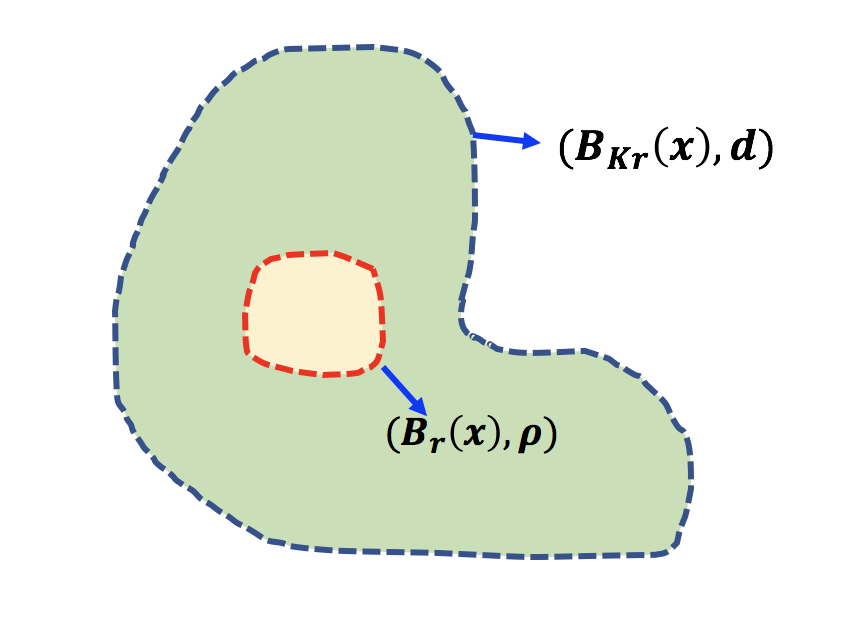
\includegraphics[width=8cm]{week1/f_3_1}
\caption{The open ball $(B_r(x),\rho)$ is contained by the open ball $(B_{Kr}(x),d)$}
\end{figure}
For each $x\in X$, consider the open ball $(B_r(x),\rho)$ and the open ball $(B_{Kr}(x),d)$:
\[
\begin{array}{ll}
B_r(x)=\{y\mid \rho(x,y)<r\},
&
B_{Kr}(x)=\{z\mid d(x,z)<Kr\}.
\end{array}
\]
For $y\in (B_r(x),\rho)$, we have $d(x,y)<K\rho(x,y)<Kr$, which implies $y\in (B_{Kr}(x),d)$, i.e, $(B_r(x),\rho)\subseteq (B_{Kr}(x),d)$ for any $x\in X$ and $r>0$.

\end{remark}
\begin{example}
\begin{enumerate}
\item
$d_1,d_2,d_\infty$ in $\mathbb{R}^n$ are equivalent
\begin{align*}
d_1(\bm x,\bm y)&\le d_\infty(\bm x,\bm y)\le nd_1(\bm x,\bm y)\\
d_2(\bm x,\bm y)&\le d_\infty(\bm x,\bm y)\le\sqrt{n}d_2(\bm x,\bm y)
\end{align*}
We use two relation depiected in the figure below to explain these two inequalities:
\begin{figure}[H]
\centering
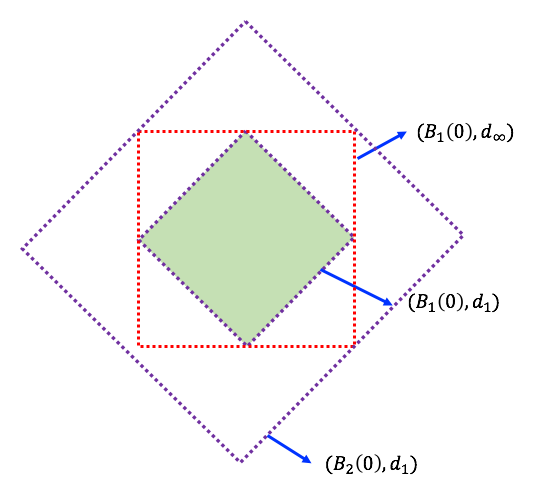
\includegraphics[width=8cm]{week1/f_3_2}
\caption{The diagram for the relation $(B_1(x),d_1)\subseteq(B_\infty(x),d_\infty)\subseteq (B_2(x),d_1)$ on $\mathbb{R}^2$}
\end{figure}
\begin{figure}[H]
\centering
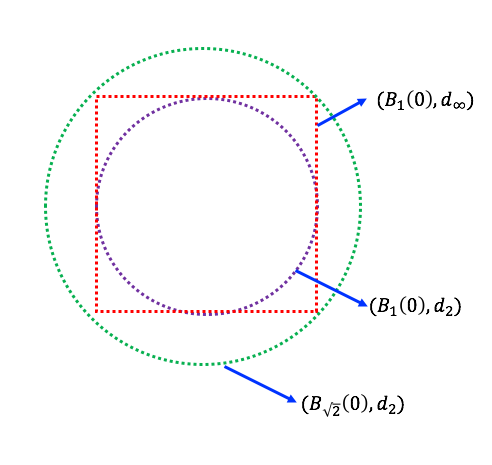
\includegraphics[width=8cm]{week1/f_3_3}
\caption{The diagram for the relation $(B_1(x),d_2)\subseteq(B_\infty(x),d_\infty)\subseteq (B_{\sqrt{2}}(x),d_2)$ on $\mathbb{R}^2$}
\end{figure}
It's easy to conclude the simple generalization for example~(\ref{Exp:1:16}):
\begin{proposition}
If $d$ and $\rho$ are equivalent, then 
\[
\lim_{n\to\infty}d(x_n,x)=0\Longleftrightarrow
\lim_{n\to\infty}\rho(x_n,x)=0
\]
\end{proposition}
Note that this does not necessarily hold for topology spaces.
\item
Consider $d_1,d_\infty$ in $\mathcal{C}[a,b]$:
\[
d_1(f,g):=\int_a^b|f-g|\diff x\le
\int_a^b\sup_{[a,b]}|f-g|\diff x=(b-a)d_\infty(f,g),
\]
i.e., $d_\infty$ is stronger than $d_1$. Question: Are they equivalent? \emph{No}.
\begin{proof}[Justification]
Consider $f_n(x)=n^2x^n(1-x)$ for $x\in[0,1]$. Check that
\[
\lim_{n\to\infty}d_1(f_n(x),0)=0,\quad
\mbox{but }d_\infty(f_n(x),0)\to\infty
\]
The peak of $f_n$ may go to infinite, while the integration converges to zero, i.e., there is no $K>0$ such that $d_{\infty}(f_n,0) < K d_1(f_n,0),\forall n\in\mathbb{N}$.
\end{proof}
We will discuss this topic at Lebsegue integration again.
\end{enumerate}
\end{example}
\subsection{Continuity}
\begin{definition}[Continuity]
Let $f:(X,d)\to(Y,d)$ be a function and $x_0\in X$. Then $f$ is continuous at $x_0$ if 
$\forall\varepsilon>0$, there exists $\delta>0$ such that
\[
d(x,x_0)<\delta\implies
\rho(f(x),f(x_0))<\varepsilon
\]
The function $f$ is continuous in $X$ if $f$ is continuous for all $x_0\in X$.
\end{definition}
\begin{proposition}\label{Pro:1:12}
The function $f$ is continuous at $x$ if and only if for all $\{x_n\}\to x$ under $d$, $f(x_n)\to f(x)$ under $\rho$.
\end{proposition}
\begin{proof}
\textit{Necessity:}
Given $\varepsilon>0$, by continuity, 
\begin{equation}\label{Eq:1:3}
d(x,x')<\delta\implies \rho(f(x'),f(x))<\varepsilon.
\end{equation}
Consider the sequence $\{x_n\}\to x$, then there exists $N$ such that $d(x_n,x)<\delta$ for $\forall n\ge N$. By applying (\ref{Eq:1:3}), $\rho(f(x_n),f(x))<\varepsilon$ for $\forall n\ge N$, i.e., $f(x_n)\to f(x)$.

\textit{Sufficiency}:
Assume that $f$ is not continuous at $x$, then there exists $\varepsilon_0$ such that for $\delta_n=\frac{1}{n}$, there exists $x_n$ such that
\[
d(x_n,x)<\delta_n,\mbox{ but }\rho(f(x_n),f(x))>\varepsilon_0.
\]
Then $\{x_n\}\to x$ by our construction, while $\{f(x_n)\}$ does not converge to $f(x)$, which is a contradiction.
\end{proof}
\begin{corollary}
If the function $f:(X,d)\to(Y,\rho)$ is continuous at $x$, the function $g:(Y,\rho)\to(Z,m)$ is continuous at $f(x)$,
then $g\circ f:(X,d)\to(Z,m)$ is continuous at $x$.
\end{corollary}
\begin{proof}
Note that
\[
\{x_n\}\to x
\xLongrightarrow{(a)}
\{f(x_n)\}\to f(x)
\xLongrightarrow{(b)}
\{g(f(x_n))\}\to g(f(x))
\xLongrightarrow{(c)}
g\circ f\mbox{ is continuous at $x$}.
\]
where $(a),(b),(c)$ are all by proposition~(\ref{Pro:1:12}).
\end{proof}
\subsection{Open and Closed Sets}
We have open/closed intervals in $\mathbb{R}$, and they are important in some theorems (e.g, continuous functions bring closed intervals to closed intervals).
\begin{definition}[Open]
Let $(X,d)$ be a metric space.  A set $U\subseteq X$ is open if for each $x\in U$, there exists $\rho_x>0$ such that $B_{\rho_x}(x)\subseteq U$. The empty set $\emptyset$ is defined to be open.
\end{definition}
\begin{example}
Let $(\mathbb{R},d_2\mbox{ or }d_\infty)$ be a metric space. The set $U=(a,b)$ is open.
\end{example}
\begin{proposition}
\begin{enumerate}
\item
Let $(X,d)$ be a metric space. Then all open balls $B_r(x)$ are open
\item
All open sets in $X$ can be written as a union of open balls.
\end{enumerate}
\end{proposition}
\begin{proof}
\begin{enumerate}
\item
Let $y\in B_r(x)$, i.e., $d(x,y):=q<r$. Consider the open ball $B_{(r-q)/2}(y)$. It suffices to show $B_{(r-q)/2}(y)\subseteq B_r(x)$. For any $z\in B_{(r-q)/2}(y)$,
\[
d(x,z)\le d(x,y)+d(y,z)<q+\frac{r-q}{2}=\frac{r+q}{2}<r.
\]
The proof is complete.
\item
Let $U\subseteq X$ be open, i.e., for $\forall x\in U$, there exists $\varepsilon_x>0$ such that $B_{\varepsilon_x}(x)\subseteq U$. Therefore
\[
\{x\}\subseteq B_{\varepsilon_x}(x)\subseteq U,\forall x\in U
\]
which implies
\[
U=\bigcup_{x\in U}\{x\}\subseteq \bigcup_{x\in U}B_{\varepsilon_x}(x)\subseteq U,
\]
i.e., $U=\bigcup_{x\in U}B_{\varepsilon_x}(x)$.
\end{enumerate}
\end{proof}

















\section{Wednesday for MAT4002}\index{Monday_lecture}
\subsection{Remarks on product space} 
\paragraph{Reviewing}
\begin{itemize}
\item
Product Topology: For topological space $(X,\mathcal{T}_X)$ and $(Y,\mathcal{Y})$, define the basis
\[
\mathcal{B}_{X\times Y}=\{U\times V\mid U\in\mathcal{T}_X,V\in\mathcal{T}_Y\}
\]
and the family of union of subsets in $\mathcal{B}_{X\times Y}$ forms a product topology.
\end{itemize}
\begin{proposition}
a ring torus is homeomorphic to the Cartesian product of two circles, say $S^1\times S^1\cong T$.
\end{proposition}
 \begin{proof}
 Define a mapping $f:[0,2\pi]\times [0,2\pi]\to T$ as
 \[
 f(\theta,\phi)=\begin{pmatrix}
(R+r\cos\theta)\cos\phi,
&
(R+r\cos\theta)\sin\phi,
&
r\sin\theta
\end{pmatrix}
 \]
Define $i:T\to\mathbb{R}^3$, we imply
 \[
 i\circ f:[0,2\pi]\times[0,2\pi]\to\mathbb{R}^3\ \text{is continuous}
 \]
 Therefore we imply $f:[0,2\pi]\times [0,2\pi]\to T$ is continuous. Together with the condition that 
\[
\left\{
\begin{aligned}
f(0,y)&=f(2\pi,y)\\
f(x,0)&=f(x,2\pi)
\end{aligned}
\right.
\]
we imply the function $f:S^1\times S^1\to T$ is continuous.
We can also show it is bijective. We can also show $f^{-1}$ is continuous.
 \end{proof}
 
\begin{proposition}
\begin{enumerate}
\item
Let $X\times Y$ be endowed with product topology. 
The projection mappings defined as
\begin{align*}
p_X:&X\times Y\to X,\ \text{with }p_X(x,y) = x\\
p_Y:&X\times Y\to Y,\ \text{with }p_Y(x,y)=y
\end{align*}
are continuous.
\item
(an equivalent definition for product topology)
The product topology is the \emph{coarest topology} on $X\times Y$ such that $p_X$ and $p_Y$ are both continuous.
\item
(an equivalent definition for product topology)
Let $Z$ be a topological space, then the product topology is the unique topology that the red and the blue line in the diagram commutes:
\begin{figure}[H]
\centering
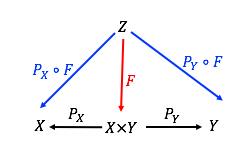
\includegraphics[width=6cm]{week3/p_3}
\caption{Diagram summarizing the statement~(*)}
\end{figure}
namely,
\begin{quotation}
\textit{
the mapping $F:Z\to X\times Y$ is continuous iff both $P_X\circ F:Z\to X$ and $P_Y\circ F:Z\to Y$ are continuous}. (*)
\end{quotation}
\end{enumerate}
\end{proposition}
\begin{proof}
\begin{enumerate}
\item
For any open $U$, we imply $p_X^{-1}(U)=U\times Y\in\mathcal{B}_{X\times Y}\subseteq\mathcal{T}_{X\times Y}$, i.e., $p_X^{-1}(U)$ is open. The same goes for $p_Y$.
\item
It suffices to show any topology $\mathcal{T}$ that meets the condition in (2) must contain $\mathcal{T}_{\text{product}}$. We imply that for $\forall U\in\mathcal{T}_X,V\in\mathcal{T}_Y$, 
\[
\left\{
\begin{aligned}
p_X^{-1}(U)&=U\times X\in\mathcal{T}\\
p_Y^{-1}(V)&=X\times V\in\mathcal{T}
\end{aligned}
\right.
\implies
(U\times Y)\cap(X\times V)=(U\cap X)\times (Y\cap V)=U\times V\in\mathcal{T},
\]
which implies $\mathcal{B}_{X\times Y}\subseteq\mathcal{T}$. Since $\mathcal{T}$ is closed for union operation on subsets, we imply $\mathcal{T}_{\text{product topology}}\subseteq\mathcal{T}$.
\item
\begin{enumerate}
\item
Firstly show that $\mathcal{T}_{\text{product}}$ satisfies (*).
\begin{itemize}
\item
For the forward direction, by (1) we imply both $p_X\circ F$ and $p_Y\circ F$ are continuous, since the composition of continuous functions are continuous as well.
\item
For the reverse direction, for $\forall U\times\mathcal{T}_X,V\in\mathcal{T}_Y$,
\[
F^{-1}(U\times V)=(p_X\circ F)^{-1}(X)\cap (p_Y\circ F)^{-1}(Y),
\]
which is open due to the continuity of $p_X\circ F$ and $p_Y\circ F$.
\end{itemize}
\item
Then we show the uniqueness of $\mathcal{T}_{\text{product}}$. Let $\mathcal{T}$ be another topology $X\times Y$ satisfying (*).
\begin{itemize}
\item
Take $Z=(X\times Y,\mathcal{T})$, and consider the identity mapping $F=\text{id}:Z\to Z$, which is continuous. Therefore $p_X\circ\text{id}$ and $p_Y\circ\text{id}$ are continuous, i.e., $p_X$ and $p_Y$ are continuous. By (2) we imply $\mathcal{T}_{\text{product}}\subseteq\mathcal{T}$.
\item
Take $Z=(X\times Y,\mathcal{T}_{\text{product}})$, and consider the identity mapping $F=\text{id}:Z\to Z$. Note that $p_X\circ F=p_X$ and $p_Y\circ F=p_Y$, which is continuous by (1). Therefore, the identity mapping $F:(X\times Y,\mathcal{T}_{\text{product}})\to(X\times Y,\mathcal{T})$ is continuous, which implies
\[
U=\text{id}^{-1}(U)\subseteq\mathcal{T}_{\text{product}}\ \text{for }\forall U\in\mathcal{T},
\]
i.e., $\mathcal{T}\subseteq\mathcal{T}_{\text{product}}.$
\end{itemize}
The proof is complete.
\end{enumerate}


\end{enumerate}
\end{proof}

\begin{definition}[Disjoint Union]
Let $X\times Y$ be two topological spaces, then the \emph{disjoint union} of $X$ and $Y$ is
\[
X\coprod Y:=(X\times\{0\})\cup(Y\times\{1\})
\]
\end{definition}
\begin{remark}
\begin{enumerate}
\item
We define that $U$ is open in $X\coprod Y$ if
\begin{enumerate}
\item
$U\cap(X\times\{0\})$ is open in $X\times\{0\}$; and
\item
$U\cap(Y\times\{1\})$ is open in $Y\times\{1\}$.
\end{enumerate}
We also need to show the well-definedness for this definition.
\item
$S$ is open in $X\coprod Y$ iff $S$ can be expressed as
\[
S=(U\times\{0\})\cup(V\times\{1\})
\]
where $U\subseteq X$ is open and $V\subseteq Y$ is open.
\end{enumerate}
\end{remark}


\subsection{Properties of Topological Spaces}
\subsubsection{Hausdorff Property}
\begin{definition}[First Separation Axiom]
A topological space $X$ satisfies the \emph{first separation axiom} if for any two distinct points $x\ne y\in X$, there exists open $U\ni x$ but not including $y$.
\end{definition}

\begin{proposition}
A topological space $X$ has first separation property if and only if for $\forall x\in X$, $\{x\}$ is closed in $X$.
\end{proposition}
\begin{proof}
\textit{Sufficiency.}
Suppose that $x\ne y$, then construct $U:=X\setminus\{y\}$, which is a open set that contains $x$ but not includes $y$.

\textit{Necessity.}
Take any $x\in X$, then for $\forall y\ne x$, there exists $y\in U_y$ that is open and $x\notin U_y$. Thus 
\[
\{y\}\subseteq U_y\subseteq X\setminus\{x\}
\]
which implies
\[
\bigcup_{y\in X\setminus\{x\}}\{y\}\subseteq
\bigcup_{y\in X\setminus\{x\}}U_y\subseteq
X\setminus\{x\},
\]
i.e., $X\setminus\{x\}=\bigcup_{y\in X\setminus\{x\}}U_y$ is open in $X$, i.e., $\{x\}$ is closed in $X.$
\end{proof}

\begin{definition}[Second separation Axiom]
A topological space satisfies the \emph{second separation axiom} (or $X$ is Hausdorff) if for all $x\ne y$ in $X$, there exists open sets $U,V$ such that
\[
\begin{array}{lll}
x\in U,
&
y\in V,
&
U\cap V=\emptyset
\end{array}
\]
\end{definition}

\begin{example}
All metrizable topological spaces are Hausdorff.

Suppose $d(x,y)=r>0$, then take $B_{r/2}(x)$ and $B_{r/2}(y)$
\end{example}

\begin{example}
Note that a topological space that is \emph{first separable} may not necessarily be \emph{second separable}:

Consider $\mathcal{T}_{\text{co-finite}}$, then $X$ is first separable but not Hausdorff:

Suppose on the contrary that for given $x\ne y$, there exists open sets $U,V$ such that $x\in U,y\in V$, and
\[
U\cap V=\emptyset\implies
X = X\setminus (U\cap V) = (X\setminus U)\cup(X\setminus V),
\]
implying that the union of two finite sets equals $X$, which is infinite, which is a contradiction.
\end{example}



















\chapter{Week4}
\section{Monday for MAT3040}\index{Monday_lecture}

\subsection{Quotient Spaces}

Now we aim to divide a big \emph{vector space} into many pieces of slices. 
\begin{itemize}
\item
For example, the Cartesian plane can be expressed as union of set of vertical lines as follows:
\[
\mathbb{R}^2 = \bigcup_{m\in\mathbb{R}}\left\{\begin{pmatrix}
m\\0
\end{pmatrix}+
\Span\{(0,1)\}\}
\right\}
\]
\item
Another example is that the set of integers can be expressed as union of three sets:
\[
\mathbb{Z}
=
Z_1\cup Z_2\cup Z_3,
\]
where $Z_i$ is the set of integers $z$ such that $z\text{ mod }3 = i$.
\end{itemize}

\begin{definition}[Coset]
Let $V$ be a vector space and $W\le V$. For any element $\bm v\in V$, the \emph{(right) coset} determined by $\bm v$ is the set
\[
\bm v+W:=\{\bm v+\bm w\mid\bm w\in W\}
\]
\end{definition}

For example, consider $V=\mathbb{R}^3$ and $W=\Span\{(1,2,0)\}$. Then the coset determined by $\bm v=(5,6,-3)$ can be written as
\[
\bm v+W=\left\{(5+t,6+2t,-3)\mid t\in\mathbb{R}\right\}
\]
It's interesting that the coset determined by $\bm v'=\{(4,4,-3)\}$ is exactly the same as the coset shown above:
\[
\bm v'+W=\left\{(4+t,4+2t,-3)\mid t\in\mathbb{R}\right\}=\bm v+W.
\]

Therefore, write the exact expression of $\bm v+W$ may sometimes become tedious and hard to check the equivalence. We say $\bm v$ is a \emph{representative} of a coset $\bm v+W$.

\begin{proposition}\label{pro:4:1}
Two cosets are the same iff the subtraction for the corresponding representatives is in $W$, i.e., 
\[
\bm v_1+W=\bm v_2+W
\Longleftrightarrow
\bm v_1-\bm v_2\in W
\]
\end{proposition}
\begin{proof}
\textit{Necessity.}
Suppose that $\bm v_1+W=\bm v_2+W$, then $\bm v_1+\bm w_1=\bm v_2+\bm w_2$ for some $\bm w_1,\bm w_2\in W$, which implies
\[
\bm v_1-\bm v_2=\bm w_2-\bm w_1\in W
\]
\textit{Sufficiency.}
Suppose that $\bm v_1-\bm v_2=\bm w\in W$. It suffices to show $\bm v_1+W\subseteq\bm v_2+W$.
For any $\bm v_1+\bm w'\in \bm v_1+W$, this element can be expressed as
\[
\bm v_1+\bm w'=(\bm v_2+\bm w)+\bm w'=\bm v_2+\underbrace{(\bm w+\bm w')}_{\text{belong to $W$}}\in \bm v_2+W.
\]
Therefore, $\bm v_1+W\subseteq \bm v_2+W$. Similarly we can show that $\bm v_2+W\subseteq \bm v_1+W$.
\end{proof}
\textit{Exercise: }Two cosets with representatives $\bm v_1,\bm v_2$ have no intersection iff $\bm v_1-\bm v_2\notin W$.

\begin{definition}[Quotient Space]
The \emph{quotient space} of $V$ by the subspace $W$, is the collection of all cosets $\bm v+W$, denoted by $V/ W$.
\end{definition}
To make the quotient space a vector space structure, we define the addition and scalar multiplication on $V/ W$ by:
\begin{align*}
(\bm v_1+W)+(\bm v_2+W)&:=(\bm v_1+\bm v_2)+W\\
\alpha\cdot (\bm v+W)&:=(\alpha\cdot\bm v) + W
\end{align*}

For example, consider $V=\mathbb{R}^2$ and $W=\Span\{(0,1)\}$. Then note that
\begin{align*}
\left(
\begin{pmatrix}
1\\0
\end{pmatrix}+W
\right)
+
\left(
\begin{pmatrix}
2\\0
\end{pmatrix}+W
\right)
&=
\left(
\begin{pmatrix}
3\\0
\end{pmatrix}+W
\right)\\
\pi\cdot\left(
\begin{pmatrix}
1\\0
\end{pmatrix}+W
\right)
&=
\left(
\begin{pmatrix}
\pi\\0
\end{pmatrix}+W
\right)
\end{align*}

\begin{proposition}
The addition and scalar multiplication is well-defined.
\end{proposition}
\begin{proof}
\begin{enumerate}
\item
Suppose that
\begin{equation}\label{Eq:4:1}
\left\{
\begin{aligned}
\bm v_1+W&=\bm v_1'+W\\
\bm v_2+W&=\bm v_2'+W
\end{aligned}
\right.,
\end{equation}
and we need to show that $(\bm v_1+\bm v_2)+W=(\bm v_1'+\bm v_2')+W$. 

From (\ref{Eq:4:1}) and proposition~(\ref{pro:4:1}), we imply
\[
\bm v_1-\bm v_1'\in W,\quad
\bm v_2-\bm v_2'\in W
\]
which implies
\[
(\bm v_1-\bm v_1')+(\bm v_2-\bm v_2')=(\bm v_1+\bm v_2) - (\bm v_1'+\bm v_2')\in W
\]

By proposition~(\ref{pro:4:1}) again we imply $(\bm v_1+\bm v_2)+W=(\bm v_1'+\bm v_2')+W$
\item
For scalar multiplication, similarly, we can show that $\bm v_1+W=\bm v_1'+W$ implies $\alpha\bm v_1+W=\alpha\bm v_1'+W$ for all $\alpha\in\mathbb{F}$.

\end{enumerate}

\end{proof}

\begin{proposition}
The canonical projection mapping
\[
\begin{aligned}
\pi_W:&V\to V/ W,\\
&\bm v\mapsto\bm v+W,
\end{aligned}
\]
is a \emph{surjective} \emph{linear transformation} with $\ker(\pi_W) = W$.
\end{proposition}
\begin{proof}
\begin{enumerate}
\item
First we show that $\ker(\pi_W)=W$:
\[
\pi_W(\bm v)=0\implies
\bm v+W=\bm0_{V/ W}\implies
\bm v+W=\bm0+W\implies \bm v=(\bm v-\bm0)\in W
\]
Here note that the zero element in the quotient space $V/ W$ is the coset with representative $\bm0$.
\item
For any $\bm v_0+W\in V/ W$, we can construct $\bm v_0\in V$ such that $\pi_W(\bm v_0)=\bm v_0+W$. Therefore the mapping $\pi_W$ is surjective.
\item
To show the mapping $\pi_W$ is a linear transformation, note that
\begin{align*}
\pi_W(\alpha\bm v_1+\beta\bm v_2)&=(\alpha\bm v_1+\beta\bm v_2)+W\\
&=(\alpha\bm v_1+W)+(\beta\bm v_2+W)\\
&=\alpha(\bm v_1+W)+\beta(\bm v_2+W)\\
&=\alpha\pi_W(\bm v_1)+\beta\pi_W(\bm v_2)
\end{align*}

\end{enumerate}


\end{proof}



\subsection{First Isomorphism Theorem}
The key of linear algebra is to solve the linear system $\bm A\bm x=\bm b$ with $\bm A\in\mathbb{R}^{m\times n}$. 
The general step for solving this linear system is as follows:
\begin{enumerate}
\item
Find the solution set for $\bm A\bm x=\bm0$, i.e., the set $\ker(\bm A)$
\item
Find a particular solution $\bm x_0$ such that $\bm A\bm x_0=\bm b$.
\end{enumerate}
Then the general solution set to this linear system is $\bm x_0+\ker(\bm A)$, which is a coset in the space $\mathbb{R}^n/ \ker(\bm A)$. Therefore, to solve the linear system $\bm{Ax}=\bm b$ suffices to study the quotient space $\mathbb{R}^n/ \ker(\bm A)$:

\begin{proposition}[Universal Property I]
Suppose that $T:V\to W$ is a linear transformation, and that $V'\le\ker(T)$. Then the mapping
\begin{align*}
\tilde{T}&:V/ V'\to W\\
&\bm v+V'\mapsto T(\bm v)
\end{align*}
is a well-defined linear transformation. As a result, the diagram below commutes:
\begin{figure}[H]
\centering
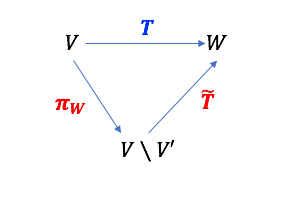
\includegraphics[width=0.5\textwidth]{week4/p_1}
\end{figure}
In other words, we have $T = \tilde{T}\circ \pi_W$.
\end{proposition}

\begin{proof}
First we show the well-definedness. Suppose that $\bm v_1+V'=\bm v_2+V'$ and suffices to show $\tilde T(\bm v_1+V')=\tilde T(\bm v_2+V')$, i.e., $T(\bm v_1)=T(\bm v_2)$. By proposition~(\ref{pro:4:1}), we imply
\[
\bm v_1-\bm v_2\in V'\le\ker(T)\implies
T(\bm v_1-\bm v_2)=\bm0\implies T(\bm v_1)-T(\bm v_2)=\bm0.
\]
Then we show $\tilde(T)$ is a linear transformation:
\begin{align*}
\tilde{T}(\alpha(\bm v_1+V')  + \beta(\bm v_2+V'))&=\tilde{T}((\alpha\bm v_1+\beta\bm v_2)+V')\\
&=T(\alpha\bm v_1+\beta\bm v_2)\\
&=\alpha T(\bm v_1)+\beta T(\bm v_2)\\
&=\alpha\tilde{T}(\bm v_1+V')+\beta\tilde{T}(\bm v_2+V')
\end{align*}
\end{proof}

Actually, if we let $V'=\ker(T)$, the mapping $\tilde{T}:V/ V'\to T(V)$ forms an isomorphism, In particular, if further $T$ is surjective, then $T(V)=W$, i.e., the mapping $\tilde{T}:V/ V'\to W$ forms an isomorphism.
\begin{theorem}[First Isomorphism Theorem]
Let $T:V\to W$ be a surjective linear transformation. Then the mapping 
\begin{align*}
\tilde{T}&:V/ \ker(T)\to W\\
&\bm v+\ker(T)\mapsto T(\bm v)
\end{align*}
is an isomorphism.
\end{theorem}
\begin{proof}
\textit{Injectivity.} Suppose that $\tilde{T}(\bm v_1+\ker(T)) = \tilde{T}(\bm v_2+\ker(T))$, then we imply
\[
T(\bm v_1)=T(\bm v_2)\implies T(\bm v_1-\bm v_2)=\bm0_W\implies\bm v_1-\bm v_2\in\ker(T),
\]
i.e., $\bm v_1+\ker(T)=\bm v_2+\ker(T)$.

\textit{Surjectivity.} For $\bm w\in W$, due to the surjectivity of $T$, we can find a $\bm v_0$ such that $T(\bm v_0)=\bm w$. Therefore, we can construct a set $\bm v_0+\ker(T)$ such that
\[
\tilde{T}(\bm v_0+\ker(T))=\bm w.
\]
\end{proof}




















\section{Monday for MAT3006}\index{Monday_lecture}
\subsection{Remarks on MCT}
\begin{example}
The MCT can help us to compute the integral
\begin{align*}
\lim_{n\to\infty}\int_{[0,n\pi]}\cos\left(\frac{x}{2n}\right)xe^{-x^2}\diff x
\end{align*}

Construct $f_n(x) = \cos\left(\frac{x}{2n}\right)xe^{-x^2}\mathcal{X}_{[0,n\pi]}$.
\begin{itemize}
\item
Since $\cos(x/2n)<\cos(x/2(n+1))$ for any $x\in[0,n\pi]$, we imply $f_n$ is monotone increasing with $n$
\item
$f_n(x)$ is integrable for all $n$.
\item
$f_n$ converges pointwise to $xe^{-x^2}\mathcal{X}_{[0,\infty)}$
\end{itemize}
Therefore, MCT I applies and
\[
\lim_{n\to\infty}\int_{[0,n\pi]}\cos\left(\frac{x}{2n}\right)xe^{-x^2}\diff x
=
\int\left(\lim_{n\to\infty}f_n\right)\diff m
\]
with
\[
\lim_{n\to\infty}f_n = xe^{-x^2}\mathcal{X}_{[0,\infty)}.
\]
Moreover, 
\begin{subequations}
\begin{align}
\int\left(\lim_{n\to\infty}f_n\right)\diff m &= 
\lim_{m\to\infty}\int_{[0,m]}xe^{-x^2}\diff x\label{Eq:12:1}\\
&=\int_0^\infty xe^{-x^2}\diff x\\
&=\frac{1}{2}
\end{align}
where (\ref{Eq:12:1}) is by applying MCT I with $g_m(x) = xe^{-x^2}\mathcal{X}_{[0,m]}$ and proposition~(\ref{pro:10:14}) to compute a Lebesgue integral by evaluating a proper Riemann integral.
\end{subequations}
\end{example}

Then we discuss the Lebesgue integral for series:

\begin{corollary}[Lebesgue Series Theorem]
Let $\{f_n\}$ be a series of measurable functions such that
\[
\sum_{n=1}^\infty\int|f_n|\diff m<\infty,
\]
then $\sum_{n=1}^kf_n$ converges to an integrable function $f = \sum_{n=1}^\infty f_n$ a.e., with
\[
\int f\diff m = \sum_{n=1}^\infty\int f_n\diff m
\]
\end{corollary}
\begin{proof}
\begin{itemize}
\item
For each $f_n$, consider 
\[
f_n = f_n^+ - f_n^-,\ \text{where $f_n^+,f_n^-$ are nonnegative}.
\]
By proposition~(\ref{pro:11:6}), 
\[
\int\sum_{n=1}^\infty f_n^+\diff m = \sum_{n=1}^\infty\int f_n^+\diff m\le \sum_{n=1}^\infty\int |f_n|\diff m<\infty.
\]
Therefore, $f^+:=\sum_{n=1}^\infty f_n^+=\lim_{k\to\infty}\sum_{n=1}^kf_n^+$ is integrable.
The same follows by replacing $f^{+}$ with $f^{-}$.
By corollary~(\ref{cor:9:6}), $f^+(x),f^-(x)<\infty,\forall x\in U$, where $U^c$ is null.
\item
Therefore, construct 
\[
f(x)=\left\{
\begin{aligned}
f^+(x)-f^-(x),&\quad x\in U\\
0,&\quad x\in U^c
\end{aligned}
\right.
\]
Moreover, for $x\in U$, 
\begin{align*}
f(x)&=\left(\lim_{k\to\infty}\sum_{n=1}^kf_n^+(x)\right)-
\left(\lim_{k\to\infty}\sum_{n=1}^kf_n^-(x)\right)\\
&=\lim_{k\to\infty}
\left(
\sum_{n=1}^kf_n^+(x)
-
\sum_{n=1}^kf_n^-(x)
\right)\\
&=\lim_{k\to\infty}\left[\sum_{n=1}^k(f_n^+(x)-f_n^-(x))\right]
\\&=
\sum_{n=1}^\infty f_n(x)
\end{align*}
where the first equality is because that both terms are finite.
\item
It follows that
\begin{subequations}
\begin{align}
\int f\diff m&=\int f^+\diff m - \int f^-\diff m\label{Eq:12:2:a}\\
&=
\int\sum_{n=1}^\infty f_n^+\diff m -\int\sum_{n=1}^\infty f_n^-\diff m\\
&=\left(\sum_{n=1}^\infty\int f_n^+\diff m\right)
-
\left(\sum_{n=1}^\infty\int f_n^-\diff m\right)\label{Eq:12:2:c}\\
&=\sum_{n=1}^\infty
\left(
\int f_n^+\diff m -\int f_n^-\diff m
\right)\label{Eq:12:2:d}\\
&=\sum_{n=1}^\infty\int f_n\diff m\label{Eq:12:2:e}
\end{align}
where (\ref{Eq:12:2:a}),(\ref{Eq:12:2:d}) is because that summation/subtraction between series holds when these series are finite; (\ref{Eq:12:2:c}) is by proposition~(\ref{pro:11:6}); (\ref{Eq:12:2:e}) is by definition of $f_n$.
\end{subequations}
\end{itemize}
\end{proof}

\begin{example}
Compute the integral
\[
\int_{(0,1]}e^{-x}x^{\alpha-1}\diff x,\ \alpha>0.
\]
\begin{itemize}
\item
Construct $f_n(x) = (-1)^n\frac{x^{\alpha+n-1}}{n!}\mathcal{X}_{(0,1]}, n\ge0$, and
\[
\sum_{n=0}^N f_n(x)\to e^{-x}x^{\alpha-1}, \ \text{pointwisely}, x\in(0,1]. 
\]
By applying MCT I,
\[
\int|f_n|\diff m=\frac{1}{(\alpha+n)n!}
\]
Therefore, 
\[
\sum_{n=0}^\infty\int|f_n|\diff m=
\sum_{n=0}^\infty\frac{1}{(\alpha+n)n!}<\infty
\]
\item
Applying the Lebesgue Series Theorem,
\[
\int_{(0,1]}e^{-x}x^{\alpha-1}\diff x = 
\int_{(0,1]}(\sum_{n=0}^\infty f_n)\diff m
=
\sum_{n=0}^\infty\int f_n\diff m=
\sum_{n=0}^\infty\frac{(-1)^n}{(\alpha+n)n!}
\]
\end{itemize}
\end{example}

\begin{remark}
It's essential to have $\sum\int|f|\diff m<\infty$ rather than $\sum\int f_n\diff m<\infty$ in the Lebesgue Series Theorem.
For example, let
\[
f_n=\frac{(-1)^{n+1}}{(n+1)}\mathcal{X}_{[n,n+1)}
\implies
\sum_{n=1}^\infty\int f_n\diff m =\log(2)<\infty
\]
However, $f:=\sum f_n$ is not integrable.
\end{remark}

\subsection{Dominated Convergence Theorem}
\begin{theorem}
Let $\{f_n\}$ be a sequence of measruable functions such that $|f_n|\le g$ a.e., and $g$ is integrable.
Suppose that $\lim_{n\to\infty}f_n(x)=f(x)$ a.e., then
\begin{enumerate}
\item
$f$ is integrable,
\item
\[
\int f\diff m =\lim_{n\to\infty}\int f_n\diff m
\]
\end{enumerate}
\end{theorem}
\begin{proof}
\begin{itemize}
\item
Observe that 
\[
|f_n|\le g\implies
\lim_{n\to\infty}|f_n|\le g\implies |f|\le g
\]
By comparison test, $g$ is integrable implies $|f|$ is integrable, and further $f$ is integrable.
\item
Consider the sequence of non-negative functions
$\{g-f_n\}_{n\in\mathbb{N}}$ and $\{g+f_n\}_{n\in\mathbb{N}}$.

By Fatou's Lemma, 
\begin{align*}
\lim_{n\to\infty}\inf\int(g-f_n)\diff m&\ge \int \lim_{n\to\infty}\inf(g-f_n)\diff m\\
&=\int(g-f)\diff m\\
&=\int g\diff m - \int f\diff m
\end{align*}
which follows that
\[
\int g\diff m - \lim_{n\to\infty}\sup\int f_n\diff m
\ge
\int g\diff m - \int f\diff m
\]
i.e.,
\[
\int f\diff m\ge  \lim_{n\to\infty}\sup\int f_n\diff m
\]
\item
Similarly, 
\[
\lim_{n\to\infty}\inf(g+f_n)\diff m\ge \int\lim_{n\to\infty}\inf(g+f_n)\diff m
=
\int g\diff m + \int f\diff m
\]
which implies
\[
 \lim_{n\to\infty}\inf\int f_n\diff m\ge\int f\diff m
\]
\end{itemize}
As a result,
\[
 \lim_{n\to\infty}\sup\int f_n\diff m
 \le
 \int f\diff m\le  \lim_{n\to\infty}\inf\int f_n\diff m,
\]
which implies
\[
\int f\diff m = \lim_n\int f_n\diff m
\]
\end{proof}

\begin{corollary}[Bounded Convergence Theorem]
Suppose that $E\in\mathcal{M}$ be such that $m(E)<\infty$.
If
\begin{itemize}
\item
$|f_n(x)|\le K<\infty$ for any $x\in E,n\in\mathbb{N}$
\item
$f_n\to f$ a.e. in $E$,
\end{itemize}
then $f$ is integrable in $E$ with
\[
\int_Ef\diff m = \lim_{n\to\infty}\int f_n\diff m
\]
\end{corollary}
\begin{proof}
Take $g=K\mathcal{X}_E$ in DCT.
\end{proof}


\begin{proposition}
Every Riemann integrable function $f$ on $[a,b]$ is Lebesgue integrable, without the condition that $f$ is continuous a.e.
\end{proposition}
\begin{proof}
Since $f$ is Riemann integrable, we imply $f$ is bounded.
We construct the Riemann lower abd upper functions with $2^n$ equal intervals, denoted as $\{\phi_n\}$ and $\{\psi_n\}$, which follows that
\begin{itemize}
\item
$\phi_n$ is monotone increasing;
$\psi_n$ is monotone decreasing;
\item
$\phi_n\le f\le \psi_n$, and
\[
\lim_{n\to\infty}\int_{[a,b]}\phi_n=\int_a^bf(x)\diff x = \lim_{n\to\infty}\int_{[a,b]}\psi_n.
\]
\end{itemize}
Construct $g=\sup_n\phi_n$ and $h=\inf_n\psi_n$.
Now we can apply the bounded convergence theorem:
\begin{itemize}
\item
$\phi_n$ is bounded on $[a,b]$
\item
$\phi_n\to g$ on $[a,b]$
\end{itemize}
which implies
$g$ is Lebesgue integrable on $[a,b]$, with 
\[
\int_{[a,b]}g\diff m = \lim_{n\to\infty}\int_{[a,b]}\phi_n\diff m=\int_a^bf(x)\diff x.
\]
Similarly, $h$ is Lebesgue integrable, with
\[
\int_{[a,b]}h\diff m = \lim_{n\to\infty}\int_{[a,b]}\psi_n\diff m=\int_a^bf(x)\diff x.
\]
Moreover, $g\le f\le h$, and
\[
\int_{[a,b]}(h-g)\diff m = \int_{[a,b]}h\diff m - \int_{[a,b]}g\diff m=\int_a^bf(x)\diff x-\int_a^bf(x)\diff x=0,
\]
which implies $h=g$ a.e., and further $f=g$ a.e., which implies
\[
\int_{[a,b]} f\diff m = \int_{[a,b]} g\diff m= \int_a^bf(x)\diff x.
\]
\end{proof}
\begin{remark}
However, an improper Riemann integral does not necessarily has the corresponding Lebesgue integral:
\[
f(x)=\sum_{n=1}^\infty (-1)^nn\cdot\mathcal{X}_{(1/(n+1),1/n]},\ x\in[0,1]
\]
In this case, $f$ is Riemann integrable but not Lebesgue integrable.
\end{remark}














\section{Monday for MAT4002}\index{Monday_lecture}

\paragraph{Reviewing}
\begin{enumerate}
\item
Topological Space $(X,\mathcal{J})$: a special class of topological space is that induced from metric space $(X,d)$:
\[
(X,\mathcal{T}),\quad\text{with }\mathcal{T}=\{\text{all open sets in $(X,d)$}\}
\]
\item
Closed Sets $(X\setminus U)$ with $U$ open.
\end{enumerate}

\begin{proposition}
Let $(X,\mathcal{T})$ be a topological space, 
\begin{enumerate}
\item
$\emptyset, X$ are closed in $X$
\item
$V_1,V_2$ closed in $X$ implies that $V_1\bigcup V_2$ closed in $X$
\item
$\{V_\alpha\mid\alpha\in\mathcal{A}\}$ closed in $X$ implies that $\bigcap_{\alpha\in\mathcal{A}}V_\alpha$ closed in $X$
\end{enumerate}
\end{proposition}
\begin{proof}
Applying the De Morgan's Law
\[
(X\setminus\bigcup_{i\in I}U_i)=\bigcap_{i\in I}(X\setminus U_i)
\]
\end{proof}

\subsection{Convergence in topological space}

\begin{definition}[Convergence]
A sequence $\{x_n\}$ of a topological space $(X,\mathcal{T})$ converges to $x\in X$ 
if $\forall U\ni x$ is open, there $\exists N$ such that $x_n\in U,\forall n\ge N$.
\end{definition}

\begin{example}
\begin{enumerate}
\item
The topology for the space $(X=\mathbb{R}^n,d_2)\to(X,\mathcal{T})$ (i.e., a topological space induced from meric space $(X=\mathbb{R}^n,d_2)$) is called a \emph{usual topology} on $\mathbb{R}^n$.

When I say $\mathbb{R}^n$ (or subset of $\mathbb{R}^n$) is a topological space, 
it is equipeed with usual topology.

Convergence of sequence in $(\mathbb{R}^n,\mathcal{T})$ is the usual convergence in analysis.

For $\mathbb{R}^n$ or metric space, the limit of sequence (if exists) is unique.

\item

Consider the topological space $(X,\mathcal{T}_{\text{indiscrete}})$. 
Take any sequence $\{x_n\}$ in $X$, it is convergent to any $x\in X$. 
Indeed, for $\forall U\ni x$ open, $U=X$. Therefore, 
\[
x_n\in U(=X),\forall n\ge1.
\]
\item

Consider the topological space $(X,\mathcal{T}_{\text{cofinite}})$, where $X$ is infinite. 
Consider $\{x_n\}$ is a sequence satisfying $m\ne n$ implies $x_m\ne x_n$. 
Then $\{x_n\}$ is convergent to any $x\in X$.

(Question: how to define openness for $\mathcal{T}_{\text{cofinite}}$ and $\mathcal{T}_{\text{indiscrete}})$?
\item

Consider the topological space $(X,\mathcal{T}_{\text{discrete}})$, 
the sequence $\{x_n\}\to x$ is equivalent to say $x_n=x$ for all sufficiently large $n$.
\end{enumerate}
\end{example}
\begin{remark}
The limit of sequences may not be unique. The reason is that ``$\mathcal{T}$ is not big enough''. We will give a criterion to make sure the limit is unique in the future. (Hausdorff)
\end{remark}
\begin{proposition}\label{pro:2:9}
If $F\subseteq(X,\mathcal{T})$ is closed, then for any convergent sequence $\{x_n\}$ in $F$, the limit(s) are also in $F$.
\end{proposition}

\begin{proof}
Let $\{x_n\}$ be a sequence in $F$ with limit $x\in X$. 
Suppose on the contrary that $x\notin F$ 
(i.e., $x\in X\setminus F$ that is open). 
There exists $N$ such that
\[
x_n\in X\setminus F,\forall n\ge N,
\]
i.e., $x_n\notin F$, which is a contradiction.
\end{proof}
\begin{remark}
The converse may not be true. If the $(X,\mathcal{T})$ is metrizable, the converse holds.

Counter-example: Consider the co-countable topological space $(X=\mathbb{R},\mathcal{T}_{\text{co-co}})$, where 
\[
\mathcal{T}_{\text{co-co}}=
\{U\mid X\setminus U\text{ is a countable set}\}
\bigcup\{\emptyset\},
\]
and $X$ is uncontable. 
Then note that $F=[0,1]\subsetneqq X$ is an un-countable set, and under co-countable topology, $F\supseteq \{x_n\}\to x$ implies $x_n=x\in F$ for all $n$.
It's clear that $X\setminus F\notin \mathcal{T}_{\text{co-co}}$, i.e., $F$ is not closed.
\end{remark}

\subsection{Interior, Closure, Boundary}
\begin{definition}\label{def:2:5}
Let $(X,\mathcal{T})$ be a topological space, and $A\subseteq X$ a subset.
\begin{enumerate}
\item
The \emph{interior} of $A$ is 
\[
A^\circ=\bigcup_{U\subseteq A,U\text{ is open}}U
\]
\item
The \emph{closure} of $A$ is
\[
\overline{A}=\bigcap_{A\subseteq V,V\text{ is closed}}V
\]
\end{enumerate}

If $\overline{A}=X$, we say that $A$ is dense in $X$.

The graph illustration of the definition above is as follows:
\begin{figure}[H]
        \begin{subfigure}[b]{0.3\textwidth}
                \centering
                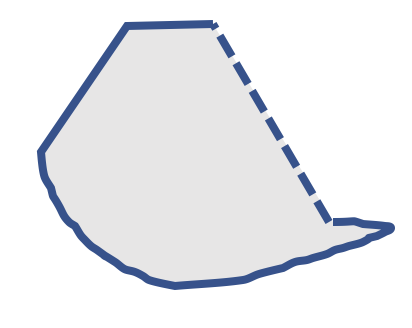
\includegraphics[width=\textwidth]{week2/p_1}
                \caption{Illustration of $A$}
                \label{fig:gull}
        \end{subfigure}%
        \begin{subfigure}[b]{0.3\textwidth}
                \centering
                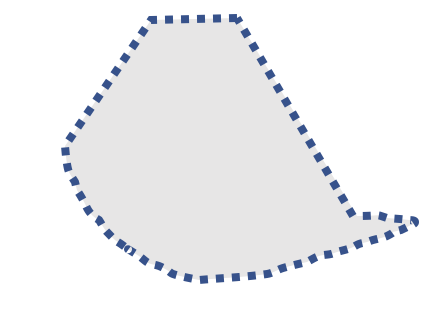
\includegraphics[width=\textwidth]{week2/p_2}
                \caption{Illustration of $A^\circ$}
                \label{fig:gull2}
        \end{subfigure}%
        \begin{subfigure}[b]{0.3\textwidth}
                \centering
                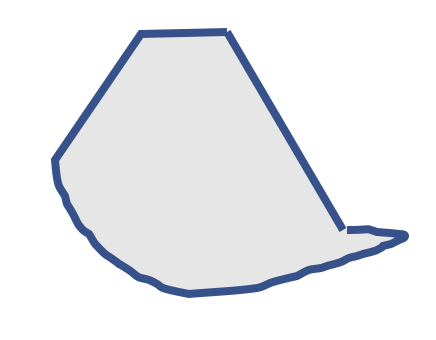
\includegraphics[width=\textwidth]{week2/p_3}
                \caption{Illustration of $\overline{A}$}
                \label{fig:tiger}
        \end{subfigure}
        \caption{Graph Illustrations}\label{fig:animals}
\end{figure}
\end{definition}
\begin{example}
\begin{enumerate}
\item

For $[a,b)\subseteq\mathbb{R}$, we have:
\[
\begin{array}{ll}
[a,b)^\circ=(a,b),
&
\overline{[a,b)}=[a,b]
\end{array}
\]

\item
For $X=\mathbb{R}$, $\mathbb{Q}^\circ=\emptyset$ and $\overline{\mathbb{Q}}=\mathbb{R}$.

\item
Consider the discrete topology $(X,\mathcal{T}_{\text{discrete}})$, we have
\[
\begin{array}{ll}
S^\circ=S,
&
\overline{S}=S
\end{array}
\]

\end{enumerate}
\end{example}

The insights behind the definition~(\ref{def:2:5}) is as follows

\begin{proposition}
\begin{enumerate}
\item
$A^\circ$ is the largest open subset of $X$ contained in $A$;

$\overline{A}$ is the smallest closed subset of $X$ containing $A$.
\item
If $A\subseteq B$, then $A^\circ\subseteq B$ and $\overline{A}\subseteq\overline{B}$
\item
$A$ is open in $X$ is equivalent to say $A^\circ = A$; $A$ is closed in $X$ is equivalent to say $\overline{A}=A$.
\end{enumerate}
\end{proposition}

\begin{example}
Let $(X,d)$ be a metric space. What's the closure of an open ball $B_r(x)$?

The direct intuition is to define the closed ball
\[
\bar B_r(x)=\{y\in X\mid d(x,y)\le r\}.
\]

Question: is $\bar B_r(x)=\overline{B_r(x)}$?
\begin{enumerate}
\item
Since $\bar B_r(x)$ is a closed subset of $X$, and 
$B_r(x)\subseteq \bar B_r(x)$, 
we imply that
\[
\overline{B_r(x)}\subseteq\bar B_r(x)
\]
\item
Howover, we may find an example such that $\overline{B_r(x)}$ is a proper subset of $\bar B_r(x)$:

Consider the discrete metric space $(X,d_{\text{discrete}})$ and for $\forall x\in X$,
\[
B_1(x)=\{x\}\implies
\overline{B_1(x)}=\{x\},\quad
\bar B_1(x)=X
\]

The equality $\bar B_r(x)=\overline{B_r(x)}$ holds when $(X,d)$ is a normed space.
\end{enumerate}
\end{example}

Here is another characterization of $\overline{A}$:

\begin{proposition}\label{pro:2:11}
\[
\overline{A}=\{x\in X\mid\forall \text{open }U\ni x, U\bigcap A\ne\emptyset\}
\]
\end{proposition}
\begin{proof}
Define
\[
S=\{x\in X\mid\forall \text{open }U\ni x, U\bigcap A\ne\emptyset\}
\]
It suffices to show that $\overline{A}=S$.
\begin{enumerate}
\item
First show that $S$ is closed:
\[
X\setminus S=\{x\in X\mid\exists U_x\ni x\text{ open s.t. }U_x\bigcap A=\emptyset\}
\]
Take $x\in X\setminus S$, we imply there exists open $U_x\ni x$ such that $U_x\bigcap A=\emptyset$. We claim $U_x\subseteq X\setminus S$:
\begin{itemize}
\item
For $\forall y\in U_x$, note that $U_x\ni y$ that is open, such that $U_x\bigcap A=\emptyset$. Therefore, $y\in X\setminus S$.
\end{itemize}

Therefore, we have $x\in U_x\subseteq X\setminus S$ for any $\forall x\in X\setminus S$.

Note that
\[
X\setminus S
=
\bigcup_{x\in X\setminus S}\{x\}\subseteq
\bigcup_{x\in X\setminus S}U_x\subseteq X\setminus S,
\]
which implies $X\setminus S=\bigcup_{x\in X\setminus S}U_x$ is open, i.e., $S$ is closed in $X$.
\item
By definition, it is clear that $A\subseteq S$:
\[
\forall a\in A,\forall\text{open }U\ni a,
U\bigcap A\supseteq\{a\}\ne\emptyset\implies a\in S.
\]
Therefore, $\overline{A}\subseteq\overline{S}=S$.
\item
Suppose on the contrary that 
there exists $y\in S\setminus\overline{A}$. 

Since $y\notin\overline{A}$, by definition, 
there exists $F\supseteq A$ closed such that 
$y\notin F$. 

Therefore, $y\in X\setminus F$ that is open, and 
\[
(X\setminus F)\bigcap A\subseteq(X\setminus A)\bigcap A=\emptyset\implies y\notin S,
\]
which is a contradiction. Therefore, $S=\overline{A}$.
\end{enumerate}
\end{proof}
\begin{definition}[accumulation point]
Let $A\subseteq X$ be a subset in a topological space. 
We call $x\in X$ are an 
\emph{accumulation point} (\emph{limit point}) of $A$ 
if
\[
\forall U\subseteq X\text{ open s.t. }
U\ni x, 
(U\setminus\{x\})\bigcap A\ne\emptyset.
\]

The set of accumulation points of $A$ is denoted as $A'$
\end{definition}
\begin{proposition}
$\overline{A}=A\bigcup A'$.
\end{proposition}

\begin{proof}
This proposition directly follows from Proposition~(\ref{pro:2:11}) and the definition of A'.
\end{proof}













\section{Wednesday for MAT3040}\index{Wednesday_lecture}
\subsection{Tensor Product for Linear Transformations}

\begin{proposition}
Suppose that $T:V\to V'$ and $S:W\to W'$ are linear transformations, then there exists an unique linear transformation 
\[
\begin{array}{ll}
T\otimes S:&V\otimes W\to V'\otimes W'\\
\text{satisfying}&(T\otimes S)(v\otimes w) = T(v)\otimes S(w)
\end{array}
\]
\end{proposition}

\begin{proof}
We construct the mapping
\[
\begin{array}{ll}
T\times S:&V\times W\to V'\otimes W'\\
\text{with}&(T\times S)(v,w) = T(v)\otimes S(w)
\end{array}
\]
This mapping is indeed bilinear: for instance, we can show that 
\[
(T\times S)(av_1+bv_2,w) = a(T\times S)(v_1,w)+b(T\times S)(v_2,w)
\]
Therefore, $T\times S\in\text{Obj}$. Since the tensor product satisfies the universal property, we imply there exists an unique linear transformation
\[
\begin{array}{ll}
T\otimes S&V\otimes W\to V'\otimes W'\\
\text{satisfying}&(T\otimes S)(v\otimes w)=T(v)\otimes S(w)
\end{array}
\]


\end{proof}
\paragraph{Notation Warning}
Does the notion $T\otimes S$ really form a tensor product, i.e., do we obtain the addictive rules for tensor product such as 
\[
(aT_1+bT_2)\otimes S = a(T_1\otimes S)+b(T_2\otimes S)?
\]


\begin{example}\label{exp:13:2}
Let $V=V'=\mathbb{F}^2$ and $W=W'=\mathbb{F}^3$.
Define the matrix-multiply mappings:
\[\left\{
\begin{array}{ll}
T:&V\to V\\
\text{with}&\bm v\mapsto\bm A\bm v\\
&\bm A=\begin{pmatrix}
a&b\\c&d
\end{pmatrix}
\end{array}\right.\qquad
\left\{
\begin{array}{ll}
S:&W\to W\\
\text{with}&\bm w\mapsto\bm B\bm w\\
&\bm B=\begin{pmatrix}
p&q&r\\
s&t&u\\
v&w&x
\end{pmatrix}
\end{array}
\right.
\]
How does $T\otimes S:V\otimes W\to V\otimes W$ look like?
\begin{itemize}
\item
Suppose $\{e_1,e_2\},\{f_1,f_2,f_3\}$ are usual basis of $V,W$, respectively.
Then the basis of $V\otimes W$ is given by:
\[
\mathcal{C}=\{e_1\otimes f_1,e_1\otimes f_2,e_1\otimes f_3,e_2\otimes f_1,e_2\otimes f_2,e_2\otimes f_3\}.
\]
\item
As a result, we can compute $(T\otimes S)(e_i\otimes f_j)$ for $i=1,2$ and $j=1,2,3$. For instance,
\begin{align*}
(T\otimes S)(e_1\otimes e_1)&=T(e_1)\otimes S(e_1)\\
&=(ae_1+ce_2)\otimes(pe_1+se_2+ve_3)\\
&=
(ap)e_1\otimes e_1+(as)e_1\otimes e_2+(av)e_1\otimes e_3+(cp)e_2\otimes e_1+(cs)e_2\otimes e_2+(cv)e_2\otimes e_3
\end{align*}
\item
Therefore, we obtain a matrix representation for the linear transformation $(T\otimes S)$:

\end{itemize}
We want a matrix representation for $(T\otimes S)$:
\[
(T\otimes S)_{\mathcal{C},\mathcal{C}}
=
\begin{pmatrix}
aB&bB\\
cB&dB
\end{pmatrix},
\]
which is a large matrix formed by taking all possible products between the elements of $\bm A$ and those of $\bm B$.
This operation is called the \emph{Kronecker Tensor Product}, see the command \textit{kron} in MATLAB for detail.


\end{example}
\begin{proposition}
More generally, given the linear operator $T:V\to V$ and $S:W\to W$, 
let $\mathcal{A}=\{v_1,\dots,v_n\},\mathcal{B}=\{w_1,\dots,w_m\}$ be a basis of $V,W$ respectively, with
\[
\begin{array}{ll}
(T)_{\mathcal{A},\mathcal{A}}=(a_{ij})
&
(S_{\mathcal{B},\mathcal{B}})=(b_{ij}):=B
\end{array}
\]
As a result, $(T\otimes S)_{\mathcal{C},\mathcal{C}}=A\otimes B$, where 
$\mathcal{C}=\{v_1\otimes w_1,\dots, v_n\otimes w_m\}$, and $A\otimes B$ denotes the Kronecker tensor product, defined as the matrix
\[
\begin{pmatrix}
a_{1,1}B&\cdots&a_{1,n}B\\
\vdots&\ddots&\vdots\\
a_{n,1}B&\cdots&a_{n,n}B
\end{pmatrix}.
\]
\end{proposition}
\begin{proof}
Following the similar procedure as in Example~(\ref{exp:13:2}) and applying the relation
\begin{align*}
(T\otimes S)(v_i\otimes w_j)&=T(v_i)\otimes S(w_j)\\
&=\left(
\sum_{k=1}^na_{ki}v_k
\right)
\otimes
\left(
\sum_{\ell=1}^mb_{\ell j}w_\ell
\right)\\
&=\sum_{k=1}^n\sum_{\ell=1}^m(a_{ki}b_{\ell j})v_k\otimes w_{\ell}
\end{align*}
\end{proof}

\begin{proposition}
The operation $T\otimes S$ satisfies all the properties of tensor product.
For example,
\begin{align*}
(aT_1+bT_2)\otimes S &= a(T_1\otimes S)+b(T_2\otimes S)\\
T\otimes(cS_1+dS_2) &= c(T\otimes S_1)+d(T\otimes S_2)
\end{align*}
Therefore, the usage of the notion ``$\otimes$'' is justified for the definition of $T\otimes S$.
\end{proposition}
\begin{proof}[Proof using matrix multiplication]
For instance, consider the operation $(T+T')\otimes S$, with $(T)_{\mathcal{A},\mathcal{A}}=(a_{ij})$, $(T')_{\mathcal{A},\mathcal{A}}=(c_{ij}), (S)_{\mathcal{B},\mathcal{B}}=B$.

We compute its matrix representation directly:
\begin{align*}
((T+T')\otimes S)_{\mathcal{C},\mathcal{C}}
&=
(T+T')_{\mathcal{A},\mathcal{A}}\otimes (S)_{\mathcal{B},\mathcal{B}}\\
&=
[(T)_{\mathcal{A},\mathcal{A}}+(T')_{\mathcal{A},\mathcal{A}}]\otimes (S)_{\mathcal{B},\mathcal{B}}\\
&=
(T)_{\mathcal{A},\mathcal{A}}\otimes (S)_{\mathcal{B},\mathcal{B}}
+
(T')_{\mathcal{A},\mathcal{A}}\otimes (S)_{\mathcal{B},\mathcal{B}}
\end{align*}
where the last equality is by the addictive rule for kronecker product for matrices.
Therefore,
\[
((T+T')\otimes S)_{\mathcal{C},\mathcal{C}}=
(T\otimes S)_{\mathcal{C},\mathcal{C}} + 
(T'\otimes S)_{\mathcal{C},\mathcal{C}}
\implies
(T+T')\otimes S
=
T\otimes S+T'\otimes S
\]
\end{proof}
\begin{proof}[Proof using basis of $T\otimes S$]
Another way of the proof is by computing 
\[
((T+T')\otimes S)(v_i\otimes w_j),
\] 
where $\{v_i\otimes w_j\mid 1\le i\le n,1\le j\le m\}$ forms a basis of $(T+T')\otimes S$:
\begin{align*}
((T+T')\otimes S)(v_i\otimes w_j)
&=(T+T')(v_i)\otimes S(w_j)\\
&=(T(v_i)+T'(v_i))\otimes S(w_j)\\
&=T(v_i)\otimes S(w_j)+T'(v_i)\otimes S(w_j)\\
&=(T\otimes S)(v_i\otimes w_j)+(T'\otimes S)(v_i\otimes w_j)
\end{align*}
Since $((T+T')\otimes S)(v_i\otimes w_j)$ coincides with $(T\otimes S + T'\otimes S)(v_i\otimes w_j)$ for all basis vectors $v_i\otimes w_j\in\mathcal{C}$, we imply
\[
(T+T')\otimes S = T\otimes S+T'\otimes S
\]
\end{proof}


\begin{proposition}
Let $A,C$ be linear operators from $V$ to $V$, and $B,D$ be linear operators from $W$ to $W$, then
\[
(A\otimes B)\circ(C\otimes D)=(AC)\otimes(BD)
\]
\end{proposition}

\begin{proposition}
Define linear operators $A:V\to V$ and $B:W\to W$ with $\dim(V),\dim(W)<\infty$.
Then
\[
\det(A\otimes B) = (\det(A))^{\dim(W)}(\det(B))^{\dim(V)}
\]
\end{proposition}

\begin{corollary}
There exists a linear transformation 
\[
\begin{array}{ll}
\Phi:&
\text{Hom}(V,V)\otimes\text{Hom}(W,W)\to
\text{Hom}(V\otimes W,V\otimes W)\\
\text{with}&A\otimes B\mapsto A\otimes B
\end{array}
\]
where the input of $\Phi$ is the tensor product of linear transformations, and the output is the linear transformation.
\end{corollary}
\begin{proof}
Construct the mapping
\[
\begin{array}{ll}
\Phi&:
\text{Hom}(V,V)\times\text{Hom}(W,W)\to
\text{Hom}(V\otimes W,V\otimes W)\\
\text{with}&\Phi(A,B)=A\otimes B
\end{array}
\]
The $\Phi$ is indeed bilinear: for instance, 
\begin{align*}
\Phi(pA+qC,B)&=(pA+qC)\otimes B\\
&=p(A\otimes B)+q(C\otimes B)\\
&=p\Phi(A,B)+q\Phi(C,B)
\end{align*}
This corollary follows from the universal property of tensor product.
\end{proof}
\begin{remark}
If assuming that $\dim(V),\dim(W)<\infty$, we imply
\begin{align*}
\dim(\text{Input space of $\Phi$})&=\dim(\text{Hom}(V,V))\dim(\text{Hom}(W,W))\\
&=
[\dim(V)\dim(V)]
\cdot
[\dim(W)\dim(W)]
=
[\dim(V)\dim(W)]^2\\
&=[\dim(V\otimes W)]^2\\
&=\dim(\text{Hom}(V\otimes W,V\otimes W))\\
&=\dim(\text{Output space of $\Phi$})
\end{align*}
Therefore, is $\Phi$ is an isomorphism?
If so, then every linear operator $\alpha:V\otimes W\to V\otimes W$ can be expressed as
\[
\alpha = A_1\otimes B_1+\cdots+A_k\otimes B_k
\]
where $A_i:V\to V$ and $B_j:W\to W$.
\end{remark}











\section{Wednesday for MAT3006}\index{Monday_lecture}
\paragraph{Reviewing}
\begin{itemize}
\item
Normed Space: a norm on a vector space
\item
Metric Space
\item
Open Ball
\end{itemize}
\subsection{Convergence of Sequences}
Since $\mathbb{R}^n$ and $\mathcal{C}[a,b]$ are both metric spaces, we can study the convergence in $\mathbb{R}^n$ and the functions defined on $[a,b]$ at the same time.

\begin{definition}[Convergence]
Let $(X,d)$ be a metric space. 
A sequence $\{x_n\}$ in $X$ is \emph{convergent} to $x$
if $\forall\varepsilon>0$, there exists $N\in\mathbb{N}$ such that
\[
d(x_n,x)<\varepsilon,\forall n\ge N.
\]
We can denote the convergence by
\[
\begin{array}{lllll}
x_n\to x,
&
\mbox{or}
&
\displaystyle
\lim_{n\to\infty}x_n=x,
&
\mbox{or}
&\displaystyle
\lim_{n\to\infty}d(x_n,x)=0
\end{array}
\]
\end{definition}
\begin{proposition}
If the limit of $\{x_n\}$ exists, then it is unique.
\end{proposition}
\begin{remark}
Note that the proposition above does not necessarily hold for topology spaces.
\end{remark}
\begin{proof}
Suppose $x_n\to x$ and $x_n\to y$, which implies
\[
0\le d(x,y)\le d(x,x_n)+d(x_n,y),\forall n
\]
Taking the limit $n\to\infty$ both sides, we imply $d(x,y)=0$, i.e., $x=y$.
\end{proof}
\begin{example}\label{Exp:1:16}
\begin{enumerate}
\item
Consider the metric space $(\mathbb{R}^k,d_\infty)$ and study the convergence
\begin{align*}
\lim_{n\to\infty}\bm x_n=\bm x&\Longleftrightarrow
\lim_{n\to\infty}\left(\max_{i=1\dots,k}|x_{n_i}-x_i|\right)=0\\
&\Longleftrightarrow
\lim_{n\to\infty}|x_{n_i}-x_i|=0,\forall i=1,\dots,k\\
&\Longleftrightarrow
\lim_{n\to\infty}x_{n_i}=x_i,
\end{align*}
i.e., the convergence defined in $d_\infty$ is the same as the convergence defined in $d_2$.
\item
Consider the convergence in the metric space $(\mathcal{C}[a,b],d_\infty)$:
\begin{align*}
\lim_{n\to\infty}f_n=f&\Longleftrightarrow
\lim_{n\to\infty}\left(\max_{[a,b]}|f_n(x)-f(x)|\right)=0\\
&\Longleftrightarrow
\forall\varepsilon>0,\forall x\in[a,b],\exists N_{\varepsilon}\mbox{ such that }|f_n(x)-f(x)|<\varepsilon,\forall n\ge N_{\varepsilon}
\end{align*}
which is equivalent to the uniform convergence of functions, i.e., the convergence defined in $d_2$.
\end{enumerate}
\end{example}
\begin{definition}[Equivalent metrics]
Let $d$ and $\rho$ be metrics on $X$. 
\begin{enumerate}
\item
We say $\rho$ is \emph{stronger} than $d$ (or $d$ is \emph{weaker} than $\rho$) if
\[
\exists K>0\mbox{ such that }d(x,y)\le K\rho(x,y),\forall x,y\in X
\]
\item
The metrics $d$ and $\rho$ are equivalent if there exists $K_1,K_2>0$ such that
\[
d(x,y)\le K_1\rho(x,y)\le K_2d(x,y)
\]
\end{enumerate}
\end{definition}
\begin{remark}
The strongerness of $\rho$ than $d$ is depiected in the graph below:
\begin{figure}[H]
\centering
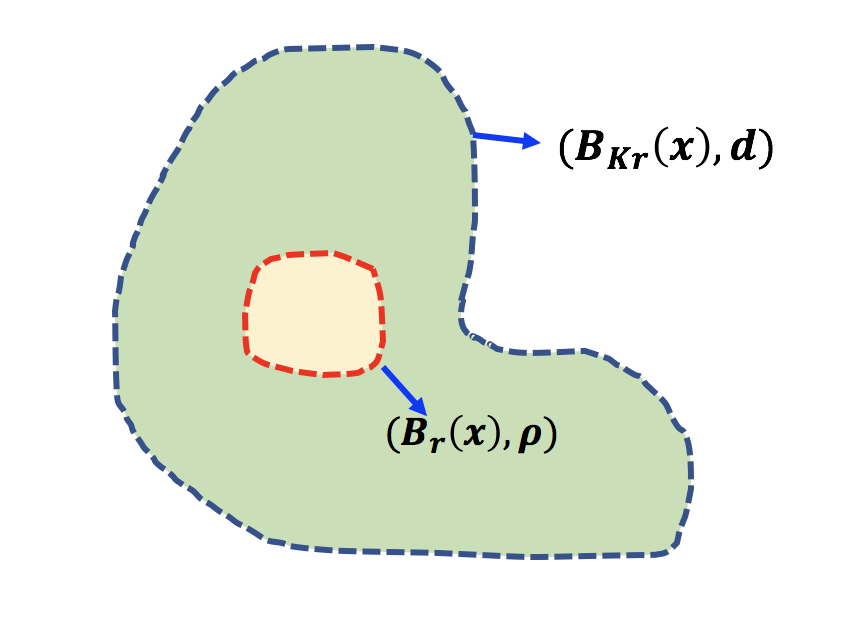
\includegraphics[width=8cm]{week1/f_3_1}
\caption{The open ball $(B_r(x),\rho)$ is contained by the open ball $(B_{Kr}(x),d)$}
\end{figure}
For each $x\in X$, consider the open ball $(B_r(x),\rho)$ and the open ball $(B_{Kr}(x),d)$:
\[
\begin{array}{ll}
B_r(x)=\{y\mid \rho(x,y)<r\},
&
B_{Kr}(x)=\{z\mid d(x,z)<Kr\}.
\end{array}
\]
For $y\in (B_r(x),\rho)$, we have $d(x,y)<K\rho(x,y)<Kr$, which implies $y\in (B_{Kr}(x),d)$, i.e, $(B_r(x),\rho)\subseteq (B_{Kr}(x),d)$ for any $x\in X$ and $r>0$.

\end{remark}
\begin{example}
\begin{enumerate}
\item
$d_1,d_2,d_\infty$ in $\mathbb{R}^n$ are equivalent
\begin{align*}
d_1(\bm x,\bm y)&\le d_\infty(\bm x,\bm y)\le nd_1(\bm x,\bm y)\\
d_2(\bm x,\bm y)&\le d_\infty(\bm x,\bm y)\le\sqrt{n}d_2(\bm x,\bm y)
\end{align*}
We use two relation depiected in the figure below to explain these two inequalities:
\begin{figure}[H]
\centering
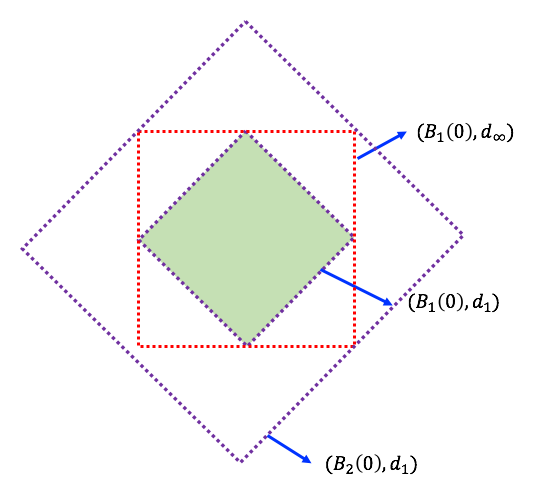
\includegraphics[width=8cm]{week1/f_3_2}
\caption{The diagram for the relation $(B_1(x),d_1)\subseteq(B_\infty(x),d_\infty)\subseteq (B_2(x),d_1)$ on $\mathbb{R}^2$}
\end{figure}
\begin{figure}[H]
\centering
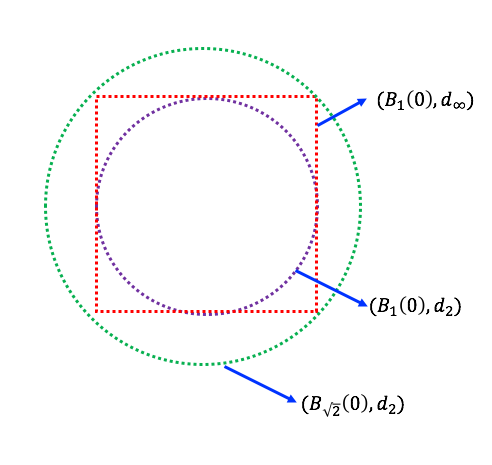
\includegraphics[width=8cm]{week1/f_3_3}
\caption{The diagram for the relation $(B_1(x),d_2)\subseteq(B_\infty(x),d_\infty)\subseteq (B_{\sqrt{2}}(x),d_2)$ on $\mathbb{R}^2$}
\end{figure}
It's easy to conclude the simple generalization for example~(\ref{Exp:1:16}):
\begin{proposition}
If $d$ and $\rho$ are equivalent, then 
\[
\lim_{n\to\infty}d(x_n,x)=0\Longleftrightarrow
\lim_{n\to\infty}\rho(x_n,x)=0
\]
\end{proposition}
Note that this does not necessarily hold for topology spaces.
\item
Consider $d_1,d_\infty$ in $\mathcal{C}[a,b]$:
\[
d_1(f,g):=\int_a^b|f-g|\diff x\le
\int_a^b\sup_{[a,b]}|f-g|\diff x=(b-a)d_\infty(f,g),
\]
i.e., $d_\infty$ is stronger than $d_1$. Question: Are they equivalent? \emph{No}.
\begin{proof}[Justification]
Consider $f_n(x)=n^2x^n(1-x)$ for $x\in[0,1]$. Check that
\[
\lim_{n\to\infty}d_1(f_n(x),0)=0,\quad
\mbox{but }d_\infty(f_n(x),0)\to\infty
\]
The peak of $f_n$ may go to infinite, while the integration converges to zero, i.e., there is no $K>0$ such that $d_{\infty}(f_n,0) < K d_1(f_n,0),\forall n\in\mathbb{N}$.
\end{proof}
We will discuss this topic at Lebsegue integration again.
\end{enumerate}
\end{example}
\subsection{Continuity}
\begin{definition}[Continuity]
Let $f:(X,d)\to(Y,d)$ be a function and $x_0\in X$. Then $f$ is continuous at $x_0$ if 
$\forall\varepsilon>0$, there exists $\delta>0$ such that
\[
d(x,x_0)<\delta\implies
\rho(f(x),f(x_0))<\varepsilon
\]
The function $f$ is continuous in $X$ if $f$ is continuous for all $x_0\in X$.
\end{definition}
\begin{proposition}\label{Pro:1:12}
The function $f$ is continuous at $x$ if and only if for all $\{x_n\}\to x$ under $d$, $f(x_n)\to f(x)$ under $\rho$.
\end{proposition}
\begin{proof}
\textit{Necessity:}
Given $\varepsilon>0$, by continuity, 
\begin{equation}\label{Eq:1:3}
d(x,x')<\delta\implies \rho(f(x'),f(x))<\varepsilon.
\end{equation}
Consider the sequence $\{x_n\}\to x$, then there exists $N$ such that $d(x_n,x)<\delta$ for $\forall n\ge N$. By applying (\ref{Eq:1:3}), $\rho(f(x_n),f(x))<\varepsilon$ for $\forall n\ge N$, i.e., $f(x_n)\to f(x)$.

\textit{Sufficiency}:
Assume that $f$ is not continuous at $x$, then there exists $\varepsilon_0$ such that for $\delta_n=\frac{1}{n}$, there exists $x_n$ such that
\[
d(x_n,x)<\delta_n,\mbox{ but }\rho(f(x_n),f(x))>\varepsilon_0.
\]
Then $\{x_n\}\to x$ by our construction, while $\{f(x_n)\}$ does not converge to $f(x)$, which is a contradiction.
\end{proof}
\begin{corollary}
If the function $f:(X,d)\to(Y,\rho)$ is continuous at $x$, the function $g:(Y,\rho)\to(Z,m)$ is continuous at $f(x)$,
then $g\circ f:(X,d)\to(Z,m)$ is continuous at $x$.
\end{corollary}
\begin{proof}
Note that
\[
\{x_n\}\to x
\xLongrightarrow{(a)}
\{f(x_n)\}\to f(x)
\xLongrightarrow{(b)}
\{g(f(x_n))\}\to g(f(x))
\xLongrightarrow{(c)}
g\circ f\mbox{ is continuous at $x$}.
\]
where $(a),(b),(c)$ are all by proposition~(\ref{Pro:1:12}).
\end{proof}
\subsection{Open and Closed Sets}
We have open/closed intervals in $\mathbb{R}$, and they are important in some theorems (e.g, continuous functions bring closed intervals to closed intervals).
\begin{definition}[Open]
Let $(X,d)$ be a metric space.  A set $U\subseteq X$ is open if for each $x\in U$, there exists $\rho_x>0$ such that $B_{\rho_x}(x)\subseteq U$. The empty set $\emptyset$ is defined to be open.
\end{definition}
\begin{example}
Let $(\mathbb{R},d_2\mbox{ or }d_\infty)$ be a metric space. The set $U=(a,b)$ is open.
\end{example}
\begin{proposition}
\begin{enumerate}
\item
Let $(X,d)$ be a metric space. Then all open balls $B_r(x)$ are open
\item
All open sets in $X$ can be written as a union of open balls.
\end{enumerate}
\end{proposition}
\begin{proof}
\begin{enumerate}
\item
Let $y\in B_r(x)$, i.e., $d(x,y):=q<r$. Consider the open ball $B_{(r-q)/2}(y)$. It suffices to show $B_{(r-q)/2}(y)\subseteq B_r(x)$. For any $z\in B_{(r-q)/2}(y)$,
\[
d(x,z)\le d(x,y)+d(y,z)<q+\frac{r-q}{2}=\frac{r+q}{2}<r.
\]
The proof is complete.
\item
Let $U\subseteq X$ be open, i.e., for $\forall x\in U$, there exists $\varepsilon_x>0$ such that $B_{\varepsilon_x}(x)\subseteq U$. Therefore
\[
\{x\}\subseteq B_{\varepsilon_x}(x)\subseteq U,\forall x\in U
\]
which implies
\[
U=\bigcup_{x\in U}\{x\}\subseteq \bigcup_{x\in U}B_{\varepsilon_x}(x)\subseteq U,
\]
i.e., $U=\bigcup_{x\in U}B_{\varepsilon_x}(x)$.
\end{enumerate}
\end{proof}

















\section{Wednesday for MAT4002}\index{Monday_lecture}
\subsection{Remarks on product space} 
\paragraph{Reviewing}
\begin{itemize}
\item
Product Topology: For topological space $(X,\mathcal{T}_X)$ and $(Y,\mathcal{Y})$, define the basis
\[
\mathcal{B}_{X\times Y}=\{U\times V\mid U\in\mathcal{T}_X,V\in\mathcal{T}_Y\}
\]
and the family of union of subsets in $\mathcal{B}_{X\times Y}$ forms a product topology.
\end{itemize}
\begin{proposition}
a ring torus is homeomorphic to the Cartesian product of two circles, say $S^1\times S^1\cong T$.
\end{proposition}
 \begin{proof}
 Define a mapping $f:[0,2\pi]\times [0,2\pi]\to T$ as
 \[
 f(\theta,\phi)=\begin{pmatrix}
(R+r\cos\theta)\cos\phi,
&
(R+r\cos\theta)\sin\phi,
&
r\sin\theta
\end{pmatrix}
 \]
Define $i:T\to\mathbb{R}^3$, we imply
 \[
 i\circ f:[0,2\pi]\times[0,2\pi]\to\mathbb{R}^3\ \text{is continuous}
 \]
 Therefore we imply $f:[0,2\pi]\times [0,2\pi]\to T$ is continuous. Together with the condition that 
\[
\left\{
\begin{aligned}
f(0,y)&=f(2\pi,y)\\
f(x,0)&=f(x,2\pi)
\end{aligned}
\right.
\]
we imply the function $f:S^1\times S^1\to T$ is continuous.
We can also show it is bijective. We can also show $f^{-1}$ is continuous.
 \end{proof}
 
\begin{proposition}
\begin{enumerate}
\item
Let $X\times Y$ be endowed with product topology. 
The projection mappings defined as
\begin{align*}
p_X:&X\times Y\to X,\ \text{with }p_X(x,y) = x\\
p_Y:&X\times Y\to Y,\ \text{with }p_Y(x,y)=y
\end{align*}
are continuous.
\item
(an equivalent definition for product topology)
The product topology is the \emph{coarest topology} on $X\times Y$ such that $p_X$ and $p_Y$ are both continuous.
\item
(an equivalent definition for product topology)
Let $Z$ be a topological space, then the product topology is the unique topology that the red and the blue line in the diagram commutes:
\begin{figure}[H]
\centering
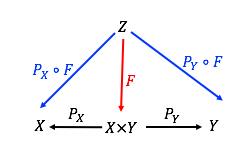
\includegraphics[width=6cm]{week3/p_3}
\caption{Diagram summarizing the statement~(*)}
\end{figure}
namely,
\begin{quotation}
\textit{
the mapping $F:Z\to X\times Y$ is continuous iff both $P_X\circ F:Z\to X$ and $P_Y\circ F:Z\to Y$ are continuous}. (*)
\end{quotation}
\end{enumerate}
\end{proposition}
\begin{proof}
\begin{enumerate}
\item
For any open $U$, we imply $p_X^{-1}(U)=U\times Y\in\mathcal{B}_{X\times Y}\subseteq\mathcal{T}_{X\times Y}$, i.e., $p_X^{-1}(U)$ is open. The same goes for $p_Y$.
\item
It suffices to show any topology $\mathcal{T}$ that meets the condition in (2) must contain $\mathcal{T}_{\text{product}}$. We imply that for $\forall U\in\mathcal{T}_X,V\in\mathcal{T}_Y$, 
\[
\left\{
\begin{aligned}
p_X^{-1}(U)&=U\times X\in\mathcal{T}\\
p_Y^{-1}(V)&=X\times V\in\mathcal{T}
\end{aligned}
\right.
\implies
(U\times Y)\cap(X\times V)=(U\cap X)\times (Y\cap V)=U\times V\in\mathcal{T},
\]
which implies $\mathcal{B}_{X\times Y}\subseteq\mathcal{T}$. Since $\mathcal{T}$ is closed for union operation on subsets, we imply $\mathcal{T}_{\text{product topology}}\subseteq\mathcal{T}$.
\item
\begin{enumerate}
\item
Firstly show that $\mathcal{T}_{\text{product}}$ satisfies (*).
\begin{itemize}
\item
For the forward direction, by (1) we imply both $p_X\circ F$ and $p_Y\circ F$ are continuous, since the composition of continuous functions are continuous as well.
\item
For the reverse direction, for $\forall U\times\mathcal{T}_X,V\in\mathcal{T}_Y$,
\[
F^{-1}(U\times V)=(p_X\circ F)^{-1}(X)\cap (p_Y\circ F)^{-1}(Y),
\]
which is open due to the continuity of $p_X\circ F$ and $p_Y\circ F$.
\end{itemize}
\item
Then we show the uniqueness of $\mathcal{T}_{\text{product}}$. Let $\mathcal{T}$ be another topology $X\times Y$ satisfying (*).
\begin{itemize}
\item
Take $Z=(X\times Y,\mathcal{T})$, and consider the identity mapping $F=\text{id}:Z\to Z$, which is continuous. Therefore $p_X\circ\text{id}$ and $p_Y\circ\text{id}$ are continuous, i.e., $p_X$ and $p_Y$ are continuous. By (2) we imply $\mathcal{T}_{\text{product}}\subseteq\mathcal{T}$.
\item
Take $Z=(X\times Y,\mathcal{T}_{\text{product}})$, and consider the identity mapping $F=\text{id}:Z\to Z$. Note that $p_X\circ F=p_X$ and $p_Y\circ F=p_Y$, which is continuous by (1). Therefore, the identity mapping $F:(X\times Y,\mathcal{T}_{\text{product}})\to(X\times Y,\mathcal{T})$ is continuous, which implies
\[
U=\text{id}^{-1}(U)\subseteq\mathcal{T}_{\text{product}}\ \text{for }\forall U\in\mathcal{T},
\]
i.e., $\mathcal{T}\subseteq\mathcal{T}_{\text{product}}.$
\end{itemize}
The proof is complete.
\end{enumerate}


\end{enumerate}
\end{proof}

\begin{definition}[Disjoint Union]
Let $X\times Y$ be two topological spaces, then the \emph{disjoint union} of $X$ and $Y$ is
\[
X\coprod Y:=(X\times\{0\})\cup(Y\times\{1\})
\]
\end{definition}
\begin{remark}
\begin{enumerate}
\item
We define that $U$ is open in $X\coprod Y$ if
\begin{enumerate}
\item
$U\cap(X\times\{0\})$ is open in $X\times\{0\}$; and
\item
$U\cap(Y\times\{1\})$ is open in $Y\times\{1\}$.
\end{enumerate}
We also need to show the well-definedness for this definition.
\item
$S$ is open in $X\coprod Y$ iff $S$ can be expressed as
\[
S=(U\times\{0\})\cup(V\times\{1\})
\]
where $U\subseteq X$ is open and $V\subseteq Y$ is open.
\end{enumerate}
\end{remark}


\subsection{Properties of Topological Spaces}
\subsubsection{Hausdorff Property}
\begin{definition}[First Separation Axiom]
A topological space $X$ satisfies the \emph{first separation axiom} if for any two distinct points $x\ne y\in X$, there exists open $U\ni x$ but not including $y$.
\end{definition}

\begin{proposition}
A topological space $X$ has first separation property if and only if for $\forall x\in X$, $\{x\}$ is closed in $X$.
\end{proposition}
\begin{proof}
\textit{Sufficiency.}
Suppose that $x\ne y$, then construct $U:=X\setminus\{y\}$, which is a open set that contains $x$ but not includes $y$.

\textit{Necessity.}
Take any $x\in X$, then for $\forall y\ne x$, there exists $y\in U_y$ that is open and $x\notin U_y$. Thus 
\[
\{y\}\subseteq U_y\subseteq X\setminus\{x\}
\]
which implies
\[
\bigcup_{y\in X\setminus\{x\}}\{y\}\subseteq
\bigcup_{y\in X\setminus\{x\}}U_y\subseteq
X\setminus\{x\},
\]
i.e., $X\setminus\{x\}=\bigcup_{y\in X\setminus\{x\}}U_y$ is open in $X$, i.e., $\{x\}$ is closed in $X.$
\end{proof}

\begin{definition}[Second separation Axiom]
A topological space satisfies the \emph{second separation axiom} (or $X$ is Hausdorff) if for all $x\ne y$ in $X$, there exists open sets $U,V$ such that
\[
\begin{array}{lll}
x\in U,
&
y\in V,
&
U\cap V=\emptyset
\end{array}
\]
\end{definition}

\begin{example}
All metrizable topological spaces are Hausdorff.

Suppose $d(x,y)=r>0$, then take $B_{r/2}(x)$ and $B_{r/2}(y)$
\end{example}

\begin{example}
Note that a topological space that is \emph{first separable} may not necessarily be \emph{second separable}:

Consider $\mathcal{T}_{\text{co-finite}}$, then $X$ is first separable but not Hausdorff:

Suppose on the contrary that for given $x\ne y$, there exists open sets $U,V$ such that $x\in U,y\in V$, and
\[
U\cap V=\emptyset\implies
X = X\setminus (U\cap V) = (X\setminus U)\cup(X\setminus V),
\]
implying that the union of two finite sets equals $X$, which is infinite, which is a contradiction.
\end{example}



















\chapter{Week4}
\section{Monday for MAT3040}\index{Monday_lecture}

\subsection{Quotient Spaces}

Now we aim to divide a big \emph{vector space} into many pieces of slices. 
\begin{itemize}
\item
For example, the Cartesian plane can be expressed as union of set of vertical lines as follows:
\[
\mathbb{R}^2 = \bigcup_{m\in\mathbb{R}}\left\{\begin{pmatrix}
m\\0
\end{pmatrix}+
\Span\{(0,1)\}\}
\right\}
\]
\item
Another example is that the set of integers can be expressed as union of three sets:
\[
\mathbb{Z}
=
Z_1\cup Z_2\cup Z_3,
\]
where $Z_i$ is the set of integers $z$ such that $z\text{ mod }3 = i$.
\end{itemize}

\begin{definition}[Coset]
Let $V$ be a vector space and $W\le V$. For any element $\bm v\in V$, the \emph{(right) coset} determined by $\bm v$ is the set
\[
\bm v+W:=\{\bm v+\bm w\mid\bm w\in W\}
\]
\end{definition}

For example, consider $V=\mathbb{R}^3$ and $W=\Span\{(1,2,0)\}$. Then the coset determined by $\bm v=(5,6,-3)$ can be written as
\[
\bm v+W=\left\{(5+t,6+2t,-3)\mid t\in\mathbb{R}\right\}
\]
It's interesting that the coset determined by $\bm v'=\{(4,4,-3)\}$ is exactly the same as the coset shown above:
\[
\bm v'+W=\left\{(4+t,4+2t,-3)\mid t\in\mathbb{R}\right\}=\bm v+W.
\]

Therefore, write the exact expression of $\bm v+W$ may sometimes become tedious and hard to check the equivalence. We say $\bm v$ is a \emph{representative} of a coset $\bm v+W$.

\begin{proposition}\label{pro:4:1}
Two cosets are the same iff the subtraction for the corresponding representatives is in $W$, i.e., 
\[
\bm v_1+W=\bm v_2+W
\Longleftrightarrow
\bm v_1-\bm v_2\in W
\]
\end{proposition}
\begin{proof}
\textit{Necessity.}
Suppose that $\bm v_1+W=\bm v_2+W$, then $\bm v_1+\bm w_1=\bm v_2+\bm w_2$ for some $\bm w_1,\bm w_2\in W$, which implies
\[
\bm v_1-\bm v_2=\bm w_2-\bm w_1\in W
\]
\textit{Sufficiency.}
Suppose that $\bm v_1-\bm v_2=\bm w\in W$. It suffices to show $\bm v_1+W\subseteq\bm v_2+W$.
For any $\bm v_1+\bm w'\in \bm v_1+W$, this element can be expressed as
\[
\bm v_1+\bm w'=(\bm v_2+\bm w)+\bm w'=\bm v_2+\underbrace{(\bm w+\bm w')}_{\text{belong to $W$}}\in \bm v_2+W.
\]
Therefore, $\bm v_1+W\subseteq \bm v_2+W$. Similarly we can show that $\bm v_2+W\subseteq \bm v_1+W$.
\end{proof}
\textit{Exercise: }Two cosets with representatives $\bm v_1,\bm v_2$ have no intersection iff $\bm v_1-\bm v_2\notin W$.

\begin{definition}[Quotient Space]
The \emph{quotient space} of $V$ by the subspace $W$, is the collection of all cosets $\bm v+W$, denoted by $V/ W$.
\end{definition}
To make the quotient space a vector space structure, we define the addition and scalar multiplication on $V/ W$ by:
\begin{align*}
(\bm v_1+W)+(\bm v_2+W)&:=(\bm v_1+\bm v_2)+W\\
\alpha\cdot (\bm v+W)&:=(\alpha\cdot\bm v) + W
\end{align*}

For example, consider $V=\mathbb{R}^2$ and $W=\Span\{(0,1)\}$. Then note that
\begin{align*}
\left(
\begin{pmatrix}
1\\0
\end{pmatrix}+W
\right)
+
\left(
\begin{pmatrix}
2\\0
\end{pmatrix}+W
\right)
&=
\left(
\begin{pmatrix}
3\\0
\end{pmatrix}+W
\right)\\
\pi\cdot\left(
\begin{pmatrix}
1\\0
\end{pmatrix}+W
\right)
&=
\left(
\begin{pmatrix}
\pi\\0
\end{pmatrix}+W
\right)
\end{align*}

\begin{proposition}
The addition and scalar multiplication is well-defined.
\end{proposition}
\begin{proof}
\begin{enumerate}
\item
Suppose that
\begin{equation}\label{Eq:4:1}
\left\{
\begin{aligned}
\bm v_1+W&=\bm v_1'+W\\
\bm v_2+W&=\bm v_2'+W
\end{aligned}
\right.,
\end{equation}
and we need to show that $(\bm v_1+\bm v_2)+W=(\bm v_1'+\bm v_2')+W$. 

From (\ref{Eq:4:1}) and proposition~(\ref{pro:4:1}), we imply
\[
\bm v_1-\bm v_1'\in W,\quad
\bm v_2-\bm v_2'\in W
\]
which implies
\[
(\bm v_1-\bm v_1')+(\bm v_2-\bm v_2')=(\bm v_1+\bm v_2) - (\bm v_1'+\bm v_2')\in W
\]

By proposition~(\ref{pro:4:1}) again we imply $(\bm v_1+\bm v_2)+W=(\bm v_1'+\bm v_2')+W$
\item
For scalar multiplication, similarly, we can show that $\bm v_1+W=\bm v_1'+W$ implies $\alpha\bm v_1+W=\alpha\bm v_1'+W$ for all $\alpha\in\mathbb{F}$.

\end{enumerate}

\end{proof}

\begin{proposition}
The canonical projection mapping
\[
\begin{aligned}
\pi_W:&V\to V/ W,\\
&\bm v\mapsto\bm v+W,
\end{aligned}
\]
is a \emph{surjective} \emph{linear transformation} with $\ker(\pi_W) = W$.
\end{proposition}
\begin{proof}
\begin{enumerate}
\item
First we show that $\ker(\pi_W)=W$:
\[
\pi_W(\bm v)=0\implies
\bm v+W=\bm0_{V/ W}\implies
\bm v+W=\bm0+W\implies \bm v=(\bm v-\bm0)\in W
\]
Here note that the zero element in the quotient space $V/ W$ is the coset with representative $\bm0$.
\item
For any $\bm v_0+W\in V/ W$, we can construct $\bm v_0\in V$ such that $\pi_W(\bm v_0)=\bm v_0+W$. Therefore the mapping $\pi_W$ is surjective.
\item
To show the mapping $\pi_W$ is a linear transformation, note that
\begin{align*}
\pi_W(\alpha\bm v_1+\beta\bm v_2)&=(\alpha\bm v_1+\beta\bm v_2)+W\\
&=(\alpha\bm v_1+W)+(\beta\bm v_2+W)\\
&=\alpha(\bm v_1+W)+\beta(\bm v_2+W)\\
&=\alpha\pi_W(\bm v_1)+\beta\pi_W(\bm v_2)
\end{align*}

\end{enumerate}


\end{proof}



\subsection{First Isomorphism Theorem}
The key of linear algebra is to solve the linear system $\bm A\bm x=\bm b$ with $\bm A\in\mathbb{R}^{m\times n}$. 
The general step for solving this linear system is as follows:
\begin{enumerate}
\item
Find the solution set for $\bm A\bm x=\bm0$, i.e., the set $\ker(\bm A)$
\item
Find a particular solution $\bm x_0$ such that $\bm A\bm x_0=\bm b$.
\end{enumerate}
Then the general solution set to this linear system is $\bm x_0+\ker(\bm A)$, which is a coset in the space $\mathbb{R}^n/ \ker(\bm A)$. Therefore, to solve the linear system $\bm{Ax}=\bm b$ suffices to study the quotient space $\mathbb{R}^n/ \ker(\bm A)$:

\begin{proposition}[Universal Property I]
Suppose that $T:V\to W$ is a linear transformation, and that $V'\le\ker(T)$. Then the mapping
\begin{align*}
\tilde{T}&:V/ V'\to W\\
&\bm v+V'\mapsto T(\bm v)
\end{align*}
is a well-defined linear transformation. As a result, the diagram below commutes:
\begin{figure}[H]
\centering
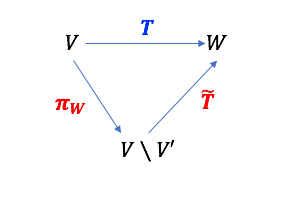
\includegraphics[width=0.5\textwidth]{week4/p_1}
\end{figure}
In other words, we have $T = \tilde{T}\circ \pi_W$.
\end{proposition}

\begin{proof}
First we show the well-definedness. Suppose that $\bm v_1+V'=\bm v_2+V'$ and suffices to show $\tilde T(\bm v_1+V')=\tilde T(\bm v_2+V')$, i.e., $T(\bm v_1)=T(\bm v_2)$. By proposition~(\ref{pro:4:1}), we imply
\[
\bm v_1-\bm v_2\in V'\le\ker(T)\implies
T(\bm v_1-\bm v_2)=\bm0\implies T(\bm v_1)-T(\bm v_2)=\bm0.
\]
Then we show $\tilde(T)$ is a linear transformation:
\begin{align*}
\tilde{T}(\alpha(\bm v_1+V')  + \beta(\bm v_2+V'))&=\tilde{T}((\alpha\bm v_1+\beta\bm v_2)+V')\\
&=T(\alpha\bm v_1+\beta\bm v_2)\\
&=\alpha T(\bm v_1)+\beta T(\bm v_2)\\
&=\alpha\tilde{T}(\bm v_1+V')+\beta\tilde{T}(\bm v_2+V')
\end{align*}
\end{proof}

Actually, if we let $V'=\ker(T)$, the mapping $\tilde{T}:V/ V'\to T(V)$ forms an isomorphism, In particular, if further $T$ is surjective, then $T(V)=W$, i.e., the mapping $\tilde{T}:V/ V'\to W$ forms an isomorphism.
\begin{theorem}[First Isomorphism Theorem]
Let $T:V\to W$ be a surjective linear transformation. Then the mapping 
\begin{align*}
\tilde{T}&:V/ \ker(T)\to W\\
&\bm v+\ker(T)\mapsto T(\bm v)
\end{align*}
is an isomorphism.
\end{theorem}
\begin{proof}
\textit{Injectivity.} Suppose that $\tilde{T}(\bm v_1+\ker(T)) = \tilde{T}(\bm v_2+\ker(T))$, then we imply
\[
T(\bm v_1)=T(\bm v_2)\implies T(\bm v_1-\bm v_2)=\bm0_W\implies\bm v_1-\bm v_2\in\ker(T),
\]
i.e., $\bm v_1+\ker(T)=\bm v_2+\ker(T)$.

\textit{Surjectivity.} For $\bm w\in W$, due to the surjectivity of $T$, we can find a $\bm v_0$ such that $T(\bm v_0)=\bm w$. Therefore, we can construct a set $\bm v_0+\ker(T)$ such that
\[
\tilde{T}(\bm v_0+\ker(T))=\bm w.
\]
\end{proof}




















\section{Monday for MAT3006}\index{Monday_lecture}
\subsection{Remarks on MCT}
\begin{example}
The MCT can help us to compute the integral
\begin{align*}
\lim_{n\to\infty}\int_{[0,n\pi]}\cos\left(\frac{x}{2n}\right)xe^{-x^2}\diff x
\end{align*}

Construct $f_n(x) = \cos\left(\frac{x}{2n}\right)xe^{-x^2}\mathcal{X}_{[0,n\pi]}$.
\begin{itemize}
\item
Since $\cos(x/2n)<\cos(x/2(n+1))$ for any $x\in[0,n\pi]$, we imply $f_n$ is monotone increasing with $n$
\item
$f_n(x)$ is integrable for all $n$.
\item
$f_n$ converges pointwise to $xe^{-x^2}\mathcal{X}_{[0,\infty)}$
\end{itemize}
Therefore, MCT I applies and
\[
\lim_{n\to\infty}\int_{[0,n\pi]}\cos\left(\frac{x}{2n}\right)xe^{-x^2}\diff x
=
\int\left(\lim_{n\to\infty}f_n\right)\diff m
\]
with
\[
\lim_{n\to\infty}f_n = xe^{-x^2}\mathcal{X}_{[0,\infty)}.
\]
Moreover, 
\begin{subequations}
\begin{align}
\int\left(\lim_{n\to\infty}f_n\right)\diff m &= 
\lim_{m\to\infty}\int_{[0,m]}xe^{-x^2}\diff x\label{Eq:12:1}\\
&=\int_0^\infty xe^{-x^2}\diff x\\
&=\frac{1}{2}
\end{align}
where (\ref{Eq:12:1}) is by applying MCT I with $g_m(x) = xe^{-x^2}\mathcal{X}_{[0,m]}$ and proposition~(\ref{pro:10:14}) to compute a Lebesgue integral by evaluating a proper Riemann integral.
\end{subequations}
\end{example}

Then we discuss the Lebesgue integral for series:

\begin{corollary}[Lebesgue Series Theorem]
Let $\{f_n\}$ be a series of measurable functions such that
\[
\sum_{n=1}^\infty\int|f_n|\diff m<\infty,
\]
then $\sum_{n=1}^kf_n$ converges to an integrable function $f = \sum_{n=1}^\infty f_n$ a.e., with
\[
\int f\diff m = \sum_{n=1}^\infty\int f_n\diff m
\]
\end{corollary}
\begin{proof}
\begin{itemize}
\item
For each $f_n$, consider 
\[
f_n = f_n^+ - f_n^-,\ \text{where $f_n^+,f_n^-$ are nonnegative}.
\]
By proposition~(\ref{pro:11:6}), 
\[
\int\sum_{n=1}^\infty f_n^+\diff m = \sum_{n=1}^\infty\int f_n^+\diff m\le \sum_{n=1}^\infty\int |f_n|\diff m<\infty.
\]
Therefore, $f^+:=\sum_{n=1}^\infty f_n^+=\lim_{k\to\infty}\sum_{n=1}^kf_n^+$ is integrable.
The same follows by replacing $f^{+}$ with $f^{-}$.
By corollary~(\ref{cor:9:6}), $f^+(x),f^-(x)<\infty,\forall x\in U$, where $U^c$ is null.
\item
Therefore, construct 
\[
f(x)=\left\{
\begin{aligned}
f^+(x)-f^-(x),&\quad x\in U\\
0,&\quad x\in U^c
\end{aligned}
\right.
\]
Moreover, for $x\in U$, 
\begin{align*}
f(x)&=\left(\lim_{k\to\infty}\sum_{n=1}^kf_n^+(x)\right)-
\left(\lim_{k\to\infty}\sum_{n=1}^kf_n^-(x)\right)\\
&=\lim_{k\to\infty}
\left(
\sum_{n=1}^kf_n^+(x)
-
\sum_{n=1}^kf_n^-(x)
\right)\\
&=\lim_{k\to\infty}\left[\sum_{n=1}^k(f_n^+(x)-f_n^-(x))\right]
\\&=
\sum_{n=1}^\infty f_n(x)
\end{align*}
where the first equality is because that both terms are finite.
\item
It follows that
\begin{subequations}
\begin{align}
\int f\diff m&=\int f^+\diff m - \int f^-\diff m\label{Eq:12:2:a}\\
&=
\int\sum_{n=1}^\infty f_n^+\diff m -\int\sum_{n=1}^\infty f_n^-\diff m\\
&=\left(\sum_{n=1}^\infty\int f_n^+\diff m\right)
-
\left(\sum_{n=1}^\infty\int f_n^-\diff m\right)\label{Eq:12:2:c}\\
&=\sum_{n=1}^\infty
\left(
\int f_n^+\diff m -\int f_n^-\diff m
\right)\label{Eq:12:2:d}\\
&=\sum_{n=1}^\infty\int f_n\diff m\label{Eq:12:2:e}
\end{align}
where (\ref{Eq:12:2:a}),(\ref{Eq:12:2:d}) is because that summation/subtraction between series holds when these series are finite; (\ref{Eq:12:2:c}) is by proposition~(\ref{pro:11:6}); (\ref{Eq:12:2:e}) is by definition of $f_n$.
\end{subequations}
\end{itemize}
\end{proof}

\begin{example}
Compute the integral
\[
\int_{(0,1]}e^{-x}x^{\alpha-1}\diff x,\ \alpha>0.
\]
\begin{itemize}
\item
Construct $f_n(x) = (-1)^n\frac{x^{\alpha+n-1}}{n!}\mathcal{X}_{(0,1]}, n\ge0$, and
\[
\sum_{n=0}^N f_n(x)\to e^{-x}x^{\alpha-1}, \ \text{pointwisely}, x\in(0,1]. 
\]
By applying MCT I,
\[
\int|f_n|\diff m=\frac{1}{(\alpha+n)n!}
\]
Therefore, 
\[
\sum_{n=0}^\infty\int|f_n|\diff m=
\sum_{n=0}^\infty\frac{1}{(\alpha+n)n!}<\infty
\]
\item
Applying the Lebesgue Series Theorem,
\[
\int_{(0,1]}e^{-x}x^{\alpha-1}\diff x = 
\int_{(0,1]}(\sum_{n=0}^\infty f_n)\diff m
=
\sum_{n=0}^\infty\int f_n\diff m=
\sum_{n=0}^\infty\frac{(-1)^n}{(\alpha+n)n!}
\]
\end{itemize}
\end{example}

\begin{remark}
It's essential to have $\sum\int|f|\diff m<\infty$ rather than $\sum\int f_n\diff m<\infty$ in the Lebesgue Series Theorem.
For example, let
\[
f_n=\frac{(-1)^{n+1}}{(n+1)}\mathcal{X}_{[n,n+1)}
\implies
\sum_{n=1}^\infty\int f_n\diff m =\log(2)<\infty
\]
However, $f:=\sum f_n$ is not integrable.
\end{remark}

\subsection{Dominated Convergence Theorem}
\begin{theorem}
Let $\{f_n\}$ be a sequence of measruable functions such that $|f_n|\le g$ a.e., and $g$ is integrable.
Suppose that $\lim_{n\to\infty}f_n(x)=f(x)$ a.e., then
\begin{enumerate}
\item
$f$ is integrable,
\item
\[
\int f\diff m =\lim_{n\to\infty}\int f_n\diff m
\]
\end{enumerate}
\end{theorem}
\begin{proof}
\begin{itemize}
\item
Observe that 
\[
|f_n|\le g\implies
\lim_{n\to\infty}|f_n|\le g\implies |f|\le g
\]
By comparison test, $g$ is integrable implies $|f|$ is integrable, and further $f$ is integrable.
\item
Consider the sequence of non-negative functions
$\{g-f_n\}_{n\in\mathbb{N}}$ and $\{g+f_n\}_{n\in\mathbb{N}}$.

By Fatou's Lemma, 
\begin{align*}
\lim_{n\to\infty}\inf\int(g-f_n)\diff m&\ge \int \lim_{n\to\infty}\inf(g-f_n)\diff m\\
&=\int(g-f)\diff m\\
&=\int g\diff m - \int f\diff m
\end{align*}
which follows that
\[
\int g\diff m - \lim_{n\to\infty}\sup\int f_n\diff m
\ge
\int g\diff m - \int f\diff m
\]
i.e.,
\[
\int f\diff m\ge  \lim_{n\to\infty}\sup\int f_n\diff m
\]
\item
Similarly, 
\[
\lim_{n\to\infty}\inf(g+f_n)\diff m\ge \int\lim_{n\to\infty}\inf(g+f_n)\diff m
=
\int g\diff m + \int f\diff m
\]
which implies
\[
 \lim_{n\to\infty}\inf\int f_n\diff m\ge\int f\diff m
\]
\end{itemize}
As a result,
\[
 \lim_{n\to\infty}\sup\int f_n\diff m
 \le
 \int f\diff m\le  \lim_{n\to\infty}\inf\int f_n\diff m,
\]
which implies
\[
\int f\diff m = \lim_n\int f_n\diff m
\]
\end{proof}

\begin{corollary}[Bounded Convergence Theorem]
Suppose that $E\in\mathcal{M}$ be such that $m(E)<\infty$.
If
\begin{itemize}
\item
$|f_n(x)|\le K<\infty$ for any $x\in E,n\in\mathbb{N}$
\item
$f_n\to f$ a.e. in $E$,
\end{itemize}
then $f$ is integrable in $E$ with
\[
\int_Ef\diff m = \lim_{n\to\infty}\int f_n\diff m
\]
\end{corollary}
\begin{proof}
Take $g=K\mathcal{X}_E$ in DCT.
\end{proof}


\begin{proposition}
Every Riemann integrable function $f$ on $[a,b]$ is Lebesgue integrable, without the condition that $f$ is continuous a.e.
\end{proposition}
\begin{proof}
Since $f$ is Riemann integrable, we imply $f$ is bounded.
We construct the Riemann lower abd upper functions with $2^n$ equal intervals, denoted as $\{\phi_n\}$ and $\{\psi_n\}$, which follows that
\begin{itemize}
\item
$\phi_n$ is monotone increasing;
$\psi_n$ is monotone decreasing;
\item
$\phi_n\le f\le \psi_n$, and
\[
\lim_{n\to\infty}\int_{[a,b]}\phi_n=\int_a^bf(x)\diff x = \lim_{n\to\infty}\int_{[a,b]}\psi_n.
\]
\end{itemize}
Construct $g=\sup_n\phi_n$ and $h=\inf_n\psi_n$.
Now we can apply the bounded convergence theorem:
\begin{itemize}
\item
$\phi_n$ is bounded on $[a,b]$
\item
$\phi_n\to g$ on $[a,b]$
\end{itemize}
which implies
$g$ is Lebesgue integrable on $[a,b]$, with 
\[
\int_{[a,b]}g\diff m = \lim_{n\to\infty}\int_{[a,b]}\phi_n\diff m=\int_a^bf(x)\diff x.
\]
Similarly, $h$ is Lebesgue integrable, with
\[
\int_{[a,b]}h\diff m = \lim_{n\to\infty}\int_{[a,b]}\psi_n\diff m=\int_a^bf(x)\diff x.
\]
Moreover, $g\le f\le h$, and
\[
\int_{[a,b]}(h-g)\diff m = \int_{[a,b]}h\diff m - \int_{[a,b]}g\diff m=\int_a^bf(x)\diff x-\int_a^bf(x)\diff x=0,
\]
which implies $h=g$ a.e., and further $f=g$ a.e., which implies
\[
\int_{[a,b]} f\diff m = \int_{[a,b]} g\diff m= \int_a^bf(x)\diff x.
\]
\end{proof}
\begin{remark}
However, an improper Riemann integral does not necessarily has the corresponding Lebesgue integral:
\[
f(x)=\sum_{n=1}^\infty (-1)^nn\cdot\mathcal{X}_{(1/(n+1),1/n]},\ x\in[0,1]
\]
In this case, $f$ is Riemann integrable but not Lebesgue integrable.
\end{remark}














\section{Monday for MAT4002}\index{Monday_lecture}

\paragraph{Reviewing}
\begin{enumerate}
\item
Topological Space $(X,\mathcal{J})$: a special class of topological space is that induced from metric space $(X,d)$:
\[
(X,\mathcal{T}),\quad\text{with }\mathcal{T}=\{\text{all open sets in $(X,d)$}\}
\]
\item
Closed Sets $(X\setminus U)$ with $U$ open.
\end{enumerate}

\begin{proposition}
Let $(X,\mathcal{T})$ be a topological space, 
\begin{enumerate}
\item
$\emptyset, X$ are closed in $X$
\item
$V_1,V_2$ closed in $X$ implies that $V_1\bigcup V_2$ closed in $X$
\item
$\{V_\alpha\mid\alpha\in\mathcal{A}\}$ closed in $X$ implies that $\bigcap_{\alpha\in\mathcal{A}}V_\alpha$ closed in $X$
\end{enumerate}
\end{proposition}
\begin{proof}
Applying the De Morgan's Law
\[
(X\setminus\bigcup_{i\in I}U_i)=\bigcap_{i\in I}(X\setminus U_i)
\]
\end{proof}

\subsection{Convergence in topological space}

\begin{definition}[Convergence]
A sequence $\{x_n\}$ of a topological space $(X,\mathcal{T})$ converges to $x\in X$ 
if $\forall U\ni x$ is open, there $\exists N$ such that $x_n\in U,\forall n\ge N$.
\end{definition}

\begin{example}
\begin{enumerate}
\item
The topology for the space $(X=\mathbb{R}^n,d_2)\to(X,\mathcal{T})$ (i.e., a topological space induced from meric space $(X=\mathbb{R}^n,d_2)$) is called a \emph{usual topology} on $\mathbb{R}^n$.

When I say $\mathbb{R}^n$ (or subset of $\mathbb{R}^n$) is a topological space, 
it is equipeed with usual topology.

Convergence of sequence in $(\mathbb{R}^n,\mathcal{T})$ is the usual convergence in analysis.

For $\mathbb{R}^n$ or metric space, the limit of sequence (if exists) is unique.

\item

Consider the topological space $(X,\mathcal{T}_{\text{indiscrete}})$. 
Take any sequence $\{x_n\}$ in $X$, it is convergent to any $x\in X$. 
Indeed, for $\forall U\ni x$ open, $U=X$. Therefore, 
\[
x_n\in U(=X),\forall n\ge1.
\]
\item

Consider the topological space $(X,\mathcal{T}_{\text{cofinite}})$, where $X$ is infinite. 
Consider $\{x_n\}$ is a sequence satisfying $m\ne n$ implies $x_m\ne x_n$. 
Then $\{x_n\}$ is convergent to any $x\in X$.

(Question: how to define openness for $\mathcal{T}_{\text{cofinite}}$ and $\mathcal{T}_{\text{indiscrete}})$?
\item

Consider the topological space $(X,\mathcal{T}_{\text{discrete}})$, 
the sequence $\{x_n\}\to x$ is equivalent to say $x_n=x$ for all sufficiently large $n$.
\end{enumerate}
\end{example}
\begin{remark}
The limit of sequences may not be unique. The reason is that ``$\mathcal{T}$ is not big enough''. We will give a criterion to make sure the limit is unique in the future. (Hausdorff)
\end{remark}
\begin{proposition}\label{pro:2:9}
If $F\subseteq(X,\mathcal{T})$ is closed, then for any convergent sequence $\{x_n\}$ in $F$, the limit(s) are also in $F$.
\end{proposition}

\begin{proof}
Let $\{x_n\}$ be a sequence in $F$ with limit $x\in X$. 
Suppose on the contrary that $x\notin F$ 
(i.e., $x\in X\setminus F$ that is open). 
There exists $N$ such that
\[
x_n\in X\setminus F,\forall n\ge N,
\]
i.e., $x_n\notin F$, which is a contradiction.
\end{proof}
\begin{remark}
The converse may not be true. If the $(X,\mathcal{T})$ is metrizable, the converse holds.

Counter-example: Consider the co-countable topological space $(X=\mathbb{R},\mathcal{T}_{\text{co-co}})$, where 
\[
\mathcal{T}_{\text{co-co}}=
\{U\mid X\setminus U\text{ is a countable set}\}
\bigcup\{\emptyset\},
\]
and $X$ is uncontable. 
Then note that $F=[0,1]\subsetneqq X$ is an un-countable set, and under co-countable topology, $F\supseteq \{x_n\}\to x$ implies $x_n=x\in F$ for all $n$.
It's clear that $X\setminus F\notin \mathcal{T}_{\text{co-co}}$, i.e., $F$ is not closed.
\end{remark}

\subsection{Interior, Closure, Boundary}
\begin{definition}\label{def:2:5}
Let $(X,\mathcal{T})$ be a topological space, and $A\subseteq X$ a subset.
\begin{enumerate}
\item
The \emph{interior} of $A$ is 
\[
A^\circ=\bigcup_{U\subseteq A,U\text{ is open}}U
\]
\item
The \emph{closure} of $A$ is
\[
\overline{A}=\bigcap_{A\subseteq V,V\text{ is closed}}V
\]
\end{enumerate}

If $\overline{A}=X$, we say that $A$ is dense in $X$.

The graph illustration of the definition above is as follows:
\begin{figure}[H]
        \begin{subfigure}[b]{0.3\textwidth}
                \centering
                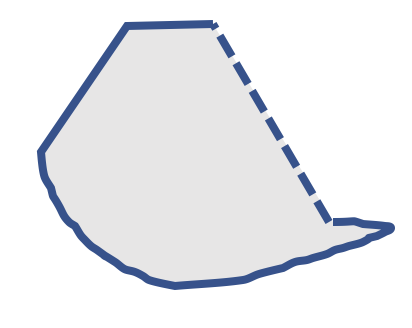
\includegraphics[width=\textwidth]{week2/p_1}
                \caption{Illustration of $A$}
                \label{fig:gull}
        \end{subfigure}%
        \begin{subfigure}[b]{0.3\textwidth}
                \centering
                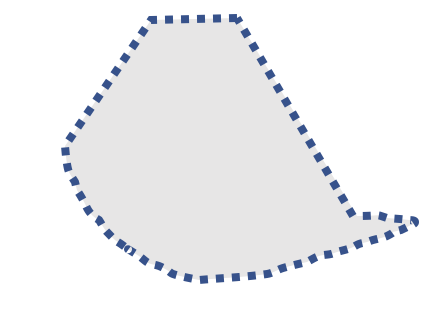
\includegraphics[width=\textwidth]{week2/p_2}
                \caption{Illustration of $A^\circ$}
                \label{fig:gull2}
        \end{subfigure}%
        \begin{subfigure}[b]{0.3\textwidth}
                \centering
                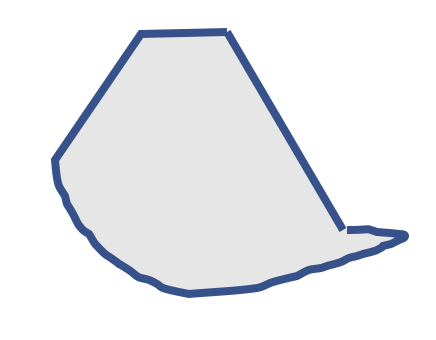
\includegraphics[width=\textwidth]{week2/p_3}
                \caption{Illustration of $\overline{A}$}
                \label{fig:tiger}
        \end{subfigure}
        \caption{Graph Illustrations}\label{fig:animals}
\end{figure}
\end{definition}
\begin{example}
\begin{enumerate}
\item

For $[a,b)\subseteq\mathbb{R}$, we have:
\[
\begin{array}{ll}
[a,b)^\circ=(a,b),
&
\overline{[a,b)}=[a,b]
\end{array}
\]

\item
For $X=\mathbb{R}$, $\mathbb{Q}^\circ=\emptyset$ and $\overline{\mathbb{Q}}=\mathbb{R}$.

\item
Consider the discrete topology $(X,\mathcal{T}_{\text{discrete}})$, we have
\[
\begin{array}{ll}
S^\circ=S,
&
\overline{S}=S
\end{array}
\]

\end{enumerate}
\end{example}

The insights behind the definition~(\ref{def:2:5}) is as follows

\begin{proposition}
\begin{enumerate}
\item
$A^\circ$ is the largest open subset of $X$ contained in $A$;

$\overline{A}$ is the smallest closed subset of $X$ containing $A$.
\item
If $A\subseteq B$, then $A^\circ\subseteq B$ and $\overline{A}\subseteq\overline{B}$
\item
$A$ is open in $X$ is equivalent to say $A^\circ = A$; $A$ is closed in $X$ is equivalent to say $\overline{A}=A$.
\end{enumerate}
\end{proposition}

\begin{example}
Let $(X,d)$ be a metric space. What's the closure of an open ball $B_r(x)$?

The direct intuition is to define the closed ball
\[
\bar B_r(x)=\{y\in X\mid d(x,y)\le r\}.
\]

Question: is $\bar B_r(x)=\overline{B_r(x)}$?
\begin{enumerate}
\item
Since $\bar B_r(x)$ is a closed subset of $X$, and 
$B_r(x)\subseteq \bar B_r(x)$, 
we imply that
\[
\overline{B_r(x)}\subseteq\bar B_r(x)
\]
\item
Howover, we may find an example such that $\overline{B_r(x)}$ is a proper subset of $\bar B_r(x)$:

Consider the discrete metric space $(X,d_{\text{discrete}})$ and for $\forall x\in X$,
\[
B_1(x)=\{x\}\implies
\overline{B_1(x)}=\{x\},\quad
\bar B_1(x)=X
\]

The equality $\bar B_r(x)=\overline{B_r(x)}$ holds when $(X,d)$ is a normed space.
\end{enumerate}
\end{example}

Here is another characterization of $\overline{A}$:

\begin{proposition}\label{pro:2:11}
\[
\overline{A}=\{x\in X\mid\forall \text{open }U\ni x, U\bigcap A\ne\emptyset\}
\]
\end{proposition}
\begin{proof}
Define
\[
S=\{x\in X\mid\forall \text{open }U\ni x, U\bigcap A\ne\emptyset\}
\]
It suffices to show that $\overline{A}=S$.
\begin{enumerate}
\item
First show that $S$ is closed:
\[
X\setminus S=\{x\in X\mid\exists U_x\ni x\text{ open s.t. }U_x\bigcap A=\emptyset\}
\]
Take $x\in X\setminus S$, we imply there exists open $U_x\ni x$ such that $U_x\bigcap A=\emptyset$. We claim $U_x\subseteq X\setminus S$:
\begin{itemize}
\item
For $\forall y\in U_x$, note that $U_x\ni y$ that is open, such that $U_x\bigcap A=\emptyset$. Therefore, $y\in X\setminus S$.
\end{itemize}

Therefore, we have $x\in U_x\subseteq X\setminus S$ for any $\forall x\in X\setminus S$.

Note that
\[
X\setminus S
=
\bigcup_{x\in X\setminus S}\{x\}\subseteq
\bigcup_{x\in X\setminus S}U_x\subseteq X\setminus S,
\]
which implies $X\setminus S=\bigcup_{x\in X\setminus S}U_x$ is open, i.e., $S$ is closed in $X$.
\item
By definition, it is clear that $A\subseteq S$:
\[
\forall a\in A,\forall\text{open }U\ni a,
U\bigcap A\supseteq\{a\}\ne\emptyset\implies a\in S.
\]
Therefore, $\overline{A}\subseteq\overline{S}=S$.
\item
Suppose on the contrary that 
there exists $y\in S\setminus\overline{A}$. 

Since $y\notin\overline{A}$, by definition, 
there exists $F\supseteq A$ closed such that 
$y\notin F$. 

Therefore, $y\in X\setminus F$ that is open, and 
\[
(X\setminus F)\bigcap A\subseteq(X\setminus A)\bigcap A=\emptyset\implies y\notin S,
\]
which is a contradiction. Therefore, $S=\overline{A}$.
\end{enumerate}
\end{proof}
\begin{definition}[accumulation point]
Let $A\subseteq X$ be a subset in a topological space. 
We call $x\in X$ are an 
\emph{accumulation point} (\emph{limit point}) of $A$ 
if
\[
\forall U\subseteq X\text{ open s.t. }
U\ni x, 
(U\setminus\{x\})\bigcap A\ne\emptyset.
\]

The set of accumulation points of $A$ is denoted as $A'$
\end{definition}
\begin{proposition}
$\overline{A}=A\bigcup A'$.
\end{proposition}

\begin{proof}
This proposition directly follows from Proposition~(\ref{pro:2:11}) and the definition of A'.
\end{proof}













\section{Wednesday for MAT3040}\index{Wednesday_lecture}
\subsection{Tensor Product for Linear Transformations}

\begin{proposition}
Suppose that $T:V\to V'$ and $S:W\to W'$ are linear transformations, then there exists an unique linear transformation 
\[
\begin{array}{ll}
T\otimes S:&V\otimes W\to V'\otimes W'\\
\text{satisfying}&(T\otimes S)(v\otimes w) = T(v)\otimes S(w)
\end{array}
\]
\end{proposition}

\begin{proof}
We construct the mapping
\[
\begin{array}{ll}
T\times S:&V\times W\to V'\otimes W'\\
\text{with}&(T\times S)(v,w) = T(v)\otimes S(w)
\end{array}
\]
This mapping is indeed bilinear: for instance, we can show that 
\[
(T\times S)(av_1+bv_2,w) = a(T\times S)(v_1,w)+b(T\times S)(v_2,w)
\]
Therefore, $T\times S\in\text{Obj}$. Since the tensor product satisfies the universal property, we imply there exists an unique linear transformation
\[
\begin{array}{ll}
T\otimes S&V\otimes W\to V'\otimes W'\\
\text{satisfying}&(T\otimes S)(v\otimes w)=T(v)\otimes S(w)
\end{array}
\]


\end{proof}
\paragraph{Notation Warning}
Does the notion $T\otimes S$ really form a tensor product, i.e., do we obtain the addictive rules for tensor product such as 
\[
(aT_1+bT_2)\otimes S = a(T_1\otimes S)+b(T_2\otimes S)?
\]


\begin{example}\label{exp:13:2}
Let $V=V'=\mathbb{F}^2$ and $W=W'=\mathbb{F}^3$.
Define the matrix-multiply mappings:
\[\left\{
\begin{array}{ll}
T:&V\to V\\
\text{with}&\bm v\mapsto\bm A\bm v\\
&\bm A=\begin{pmatrix}
a&b\\c&d
\end{pmatrix}
\end{array}\right.\qquad
\left\{
\begin{array}{ll}
S:&W\to W\\
\text{with}&\bm w\mapsto\bm B\bm w\\
&\bm B=\begin{pmatrix}
p&q&r\\
s&t&u\\
v&w&x
\end{pmatrix}
\end{array}
\right.
\]
How does $T\otimes S:V\otimes W\to V\otimes W$ look like?
\begin{itemize}
\item
Suppose $\{e_1,e_2\},\{f_1,f_2,f_3\}$ are usual basis of $V,W$, respectively.
Then the basis of $V\otimes W$ is given by:
\[
\mathcal{C}=\{e_1\otimes f_1,e_1\otimes f_2,e_1\otimes f_3,e_2\otimes f_1,e_2\otimes f_2,e_2\otimes f_3\}.
\]
\item
As a result, we can compute $(T\otimes S)(e_i\otimes f_j)$ for $i=1,2$ and $j=1,2,3$. For instance,
\begin{align*}
(T\otimes S)(e_1\otimes e_1)&=T(e_1)\otimes S(e_1)\\
&=(ae_1+ce_2)\otimes(pe_1+se_2+ve_3)\\
&=
(ap)e_1\otimes e_1+(as)e_1\otimes e_2+(av)e_1\otimes e_3+(cp)e_2\otimes e_1+(cs)e_2\otimes e_2+(cv)e_2\otimes e_3
\end{align*}
\item
Therefore, we obtain a matrix representation for the linear transformation $(T\otimes S)$:

\end{itemize}
We want a matrix representation for $(T\otimes S)$:
\[
(T\otimes S)_{\mathcal{C},\mathcal{C}}
=
\begin{pmatrix}
aB&bB\\
cB&dB
\end{pmatrix},
\]
which is a large matrix formed by taking all possible products between the elements of $\bm A$ and those of $\bm B$.
This operation is called the \emph{Kronecker Tensor Product}, see the command \textit{kron} in MATLAB for detail.


\end{example}
\begin{proposition}
More generally, given the linear operator $T:V\to V$ and $S:W\to W$, 
let $\mathcal{A}=\{v_1,\dots,v_n\},\mathcal{B}=\{w_1,\dots,w_m\}$ be a basis of $V,W$ respectively, with
\[
\begin{array}{ll}
(T)_{\mathcal{A},\mathcal{A}}=(a_{ij})
&
(S_{\mathcal{B},\mathcal{B}})=(b_{ij}):=B
\end{array}
\]
As a result, $(T\otimes S)_{\mathcal{C},\mathcal{C}}=A\otimes B$, where 
$\mathcal{C}=\{v_1\otimes w_1,\dots, v_n\otimes w_m\}$, and $A\otimes B$ denotes the Kronecker tensor product, defined as the matrix
\[
\begin{pmatrix}
a_{1,1}B&\cdots&a_{1,n}B\\
\vdots&\ddots&\vdots\\
a_{n,1}B&\cdots&a_{n,n}B
\end{pmatrix}.
\]
\end{proposition}
\begin{proof}
Following the similar procedure as in Example~(\ref{exp:13:2}) and applying the relation
\begin{align*}
(T\otimes S)(v_i\otimes w_j)&=T(v_i)\otimes S(w_j)\\
&=\left(
\sum_{k=1}^na_{ki}v_k
\right)
\otimes
\left(
\sum_{\ell=1}^mb_{\ell j}w_\ell
\right)\\
&=\sum_{k=1}^n\sum_{\ell=1}^m(a_{ki}b_{\ell j})v_k\otimes w_{\ell}
\end{align*}
\end{proof}

\begin{proposition}
The operation $T\otimes S$ satisfies all the properties of tensor product.
For example,
\begin{align*}
(aT_1+bT_2)\otimes S &= a(T_1\otimes S)+b(T_2\otimes S)\\
T\otimes(cS_1+dS_2) &= c(T\otimes S_1)+d(T\otimes S_2)
\end{align*}
Therefore, the usage of the notion ``$\otimes$'' is justified for the definition of $T\otimes S$.
\end{proposition}
\begin{proof}[Proof using matrix multiplication]
For instance, consider the operation $(T+T')\otimes S$, with $(T)_{\mathcal{A},\mathcal{A}}=(a_{ij})$, $(T')_{\mathcal{A},\mathcal{A}}=(c_{ij}), (S)_{\mathcal{B},\mathcal{B}}=B$.

We compute its matrix representation directly:
\begin{align*}
((T+T')\otimes S)_{\mathcal{C},\mathcal{C}}
&=
(T+T')_{\mathcal{A},\mathcal{A}}\otimes (S)_{\mathcal{B},\mathcal{B}}\\
&=
[(T)_{\mathcal{A},\mathcal{A}}+(T')_{\mathcal{A},\mathcal{A}}]\otimes (S)_{\mathcal{B},\mathcal{B}}\\
&=
(T)_{\mathcal{A},\mathcal{A}}\otimes (S)_{\mathcal{B},\mathcal{B}}
+
(T')_{\mathcal{A},\mathcal{A}}\otimes (S)_{\mathcal{B},\mathcal{B}}
\end{align*}
where the last equality is by the addictive rule for kronecker product for matrices.
Therefore,
\[
((T+T')\otimes S)_{\mathcal{C},\mathcal{C}}=
(T\otimes S)_{\mathcal{C},\mathcal{C}} + 
(T'\otimes S)_{\mathcal{C},\mathcal{C}}
\implies
(T+T')\otimes S
=
T\otimes S+T'\otimes S
\]
\end{proof}
\begin{proof}[Proof using basis of $T\otimes S$]
Another way of the proof is by computing 
\[
((T+T')\otimes S)(v_i\otimes w_j),
\] 
where $\{v_i\otimes w_j\mid 1\le i\le n,1\le j\le m\}$ forms a basis of $(T+T')\otimes S$:
\begin{align*}
((T+T')\otimes S)(v_i\otimes w_j)
&=(T+T')(v_i)\otimes S(w_j)\\
&=(T(v_i)+T'(v_i))\otimes S(w_j)\\
&=T(v_i)\otimes S(w_j)+T'(v_i)\otimes S(w_j)\\
&=(T\otimes S)(v_i\otimes w_j)+(T'\otimes S)(v_i\otimes w_j)
\end{align*}
Since $((T+T')\otimes S)(v_i\otimes w_j)$ coincides with $(T\otimes S + T'\otimes S)(v_i\otimes w_j)$ for all basis vectors $v_i\otimes w_j\in\mathcal{C}$, we imply
\[
(T+T')\otimes S = T\otimes S+T'\otimes S
\]
\end{proof}


\begin{proposition}
Let $A,C$ be linear operators from $V$ to $V$, and $B,D$ be linear operators from $W$ to $W$, then
\[
(A\otimes B)\circ(C\otimes D)=(AC)\otimes(BD)
\]
\end{proposition}

\begin{proposition}
Define linear operators $A:V\to V$ and $B:W\to W$ with $\dim(V),\dim(W)<\infty$.
Then
\[
\det(A\otimes B) = (\det(A))^{\dim(W)}(\det(B))^{\dim(V)}
\]
\end{proposition}

\begin{corollary}
There exists a linear transformation 
\[
\begin{array}{ll}
\Phi:&
\text{Hom}(V,V)\otimes\text{Hom}(W,W)\to
\text{Hom}(V\otimes W,V\otimes W)\\
\text{with}&A\otimes B\mapsto A\otimes B
\end{array}
\]
where the input of $\Phi$ is the tensor product of linear transformations, and the output is the linear transformation.
\end{corollary}
\begin{proof}
Construct the mapping
\[
\begin{array}{ll}
\Phi&:
\text{Hom}(V,V)\times\text{Hom}(W,W)\to
\text{Hom}(V\otimes W,V\otimes W)\\
\text{with}&\Phi(A,B)=A\otimes B
\end{array}
\]
The $\Phi$ is indeed bilinear: for instance, 
\begin{align*}
\Phi(pA+qC,B)&=(pA+qC)\otimes B\\
&=p(A\otimes B)+q(C\otimes B)\\
&=p\Phi(A,B)+q\Phi(C,B)
\end{align*}
This corollary follows from the universal property of tensor product.
\end{proof}
\begin{remark}
If assuming that $\dim(V),\dim(W)<\infty$, we imply
\begin{align*}
\dim(\text{Input space of $\Phi$})&=\dim(\text{Hom}(V,V))\dim(\text{Hom}(W,W))\\
&=
[\dim(V)\dim(V)]
\cdot
[\dim(W)\dim(W)]
=
[\dim(V)\dim(W)]^2\\
&=[\dim(V\otimes W)]^2\\
&=\dim(\text{Hom}(V\otimes W,V\otimes W))\\
&=\dim(\text{Output space of $\Phi$})
\end{align*}
Therefore, is $\Phi$ is an isomorphism?
If so, then every linear operator $\alpha:V\otimes W\to V\otimes W$ can be expressed as
\[
\alpha = A_1\otimes B_1+\cdots+A_k\otimes B_k
\]
where $A_i:V\to V$ and $B_j:W\to W$.
\end{remark}











\section{Wednesday for MAT3006}\index{Monday_lecture}
\paragraph{Reviewing}
\begin{itemize}
\item
Normed Space: a norm on a vector space
\item
Metric Space
\item
Open Ball
\end{itemize}
\subsection{Convergence of Sequences}
Since $\mathbb{R}^n$ and $\mathcal{C}[a,b]$ are both metric spaces, we can study the convergence in $\mathbb{R}^n$ and the functions defined on $[a,b]$ at the same time.

\begin{definition}[Convergence]
Let $(X,d)$ be a metric space. 
A sequence $\{x_n\}$ in $X$ is \emph{convergent} to $x$
if $\forall\varepsilon>0$, there exists $N\in\mathbb{N}$ such that
\[
d(x_n,x)<\varepsilon,\forall n\ge N.
\]
We can denote the convergence by
\[
\begin{array}{lllll}
x_n\to x,
&
\mbox{or}
&
\displaystyle
\lim_{n\to\infty}x_n=x,
&
\mbox{or}
&\displaystyle
\lim_{n\to\infty}d(x_n,x)=0
\end{array}
\]
\end{definition}
\begin{proposition}
If the limit of $\{x_n\}$ exists, then it is unique.
\end{proposition}
\begin{remark}
Note that the proposition above does not necessarily hold for topology spaces.
\end{remark}
\begin{proof}
Suppose $x_n\to x$ and $x_n\to y$, which implies
\[
0\le d(x,y)\le d(x,x_n)+d(x_n,y),\forall n
\]
Taking the limit $n\to\infty$ both sides, we imply $d(x,y)=0$, i.e., $x=y$.
\end{proof}
\begin{example}\label{Exp:1:16}
\begin{enumerate}
\item
Consider the metric space $(\mathbb{R}^k,d_\infty)$ and study the convergence
\begin{align*}
\lim_{n\to\infty}\bm x_n=\bm x&\Longleftrightarrow
\lim_{n\to\infty}\left(\max_{i=1\dots,k}|x_{n_i}-x_i|\right)=0\\
&\Longleftrightarrow
\lim_{n\to\infty}|x_{n_i}-x_i|=0,\forall i=1,\dots,k\\
&\Longleftrightarrow
\lim_{n\to\infty}x_{n_i}=x_i,
\end{align*}
i.e., the convergence defined in $d_\infty$ is the same as the convergence defined in $d_2$.
\item
Consider the convergence in the metric space $(\mathcal{C}[a,b],d_\infty)$:
\begin{align*}
\lim_{n\to\infty}f_n=f&\Longleftrightarrow
\lim_{n\to\infty}\left(\max_{[a,b]}|f_n(x)-f(x)|\right)=0\\
&\Longleftrightarrow
\forall\varepsilon>0,\forall x\in[a,b],\exists N_{\varepsilon}\mbox{ such that }|f_n(x)-f(x)|<\varepsilon,\forall n\ge N_{\varepsilon}
\end{align*}
which is equivalent to the uniform convergence of functions, i.e., the convergence defined in $d_2$.
\end{enumerate}
\end{example}
\begin{definition}[Equivalent metrics]
Let $d$ and $\rho$ be metrics on $X$. 
\begin{enumerate}
\item
We say $\rho$ is \emph{stronger} than $d$ (or $d$ is \emph{weaker} than $\rho$) if
\[
\exists K>0\mbox{ such that }d(x,y)\le K\rho(x,y),\forall x,y\in X
\]
\item
The metrics $d$ and $\rho$ are equivalent if there exists $K_1,K_2>0$ such that
\[
d(x,y)\le K_1\rho(x,y)\le K_2d(x,y)
\]
\end{enumerate}
\end{definition}
\begin{remark}
The strongerness of $\rho$ than $d$ is depiected in the graph below:
\begin{figure}[H]
\centering
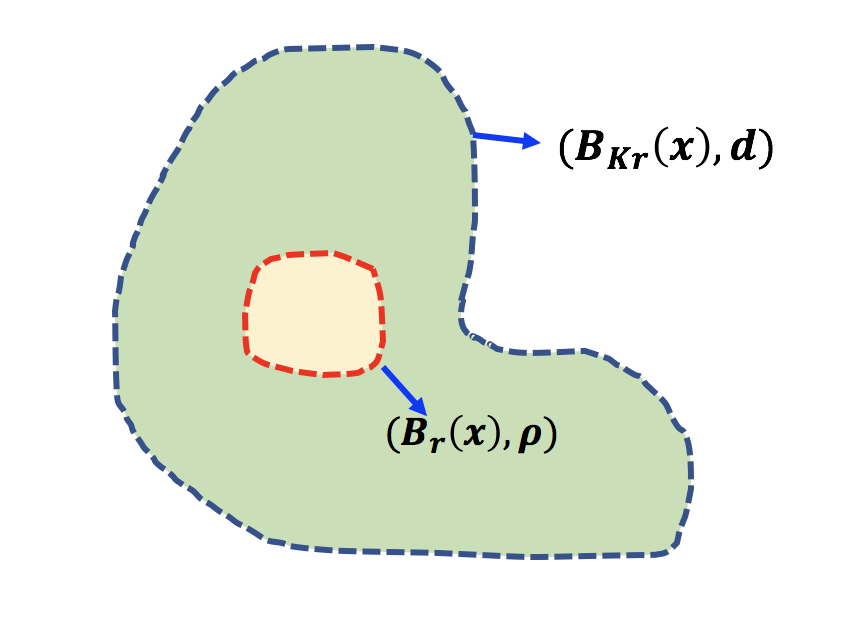
\includegraphics[width=8cm]{week1/f_3_1}
\caption{The open ball $(B_r(x),\rho)$ is contained by the open ball $(B_{Kr}(x),d)$}
\end{figure}
For each $x\in X$, consider the open ball $(B_r(x),\rho)$ and the open ball $(B_{Kr}(x),d)$:
\[
\begin{array}{ll}
B_r(x)=\{y\mid \rho(x,y)<r\},
&
B_{Kr}(x)=\{z\mid d(x,z)<Kr\}.
\end{array}
\]
For $y\in (B_r(x),\rho)$, we have $d(x,y)<K\rho(x,y)<Kr$, which implies $y\in (B_{Kr}(x),d)$, i.e, $(B_r(x),\rho)\subseteq (B_{Kr}(x),d)$ for any $x\in X$ and $r>0$.

\end{remark}
\begin{example}
\begin{enumerate}
\item
$d_1,d_2,d_\infty$ in $\mathbb{R}^n$ are equivalent
\begin{align*}
d_1(\bm x,\bm y)&\le d_\infty(\bm x,\bm y)\le nd_1(\bm x,\bm y)\\
d_2(\bm x,\bm y)&\le d_\infty(\bm x,\bm y)\le\sqrt{n}d_2(\bm x,\bm y)
\end{align*}
We use two relation depiected in the figure below to explain these two inequalities:
\begin{figure}[H]
\centering
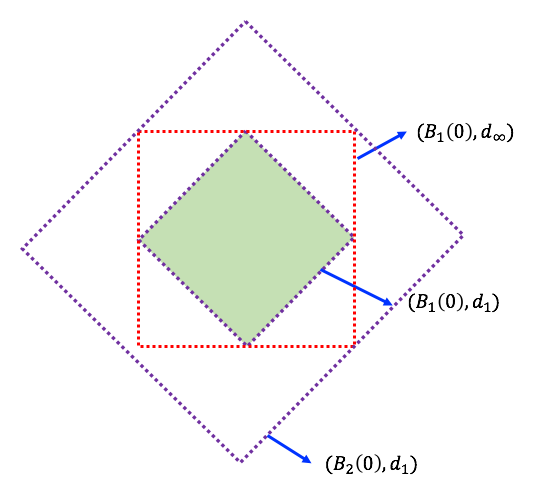
\includegraphics[width=8cm]{week1/f_3_2}
\caption{The diagram for the relation $(B_1(x),d_1)\subseteq(B_\infty(x),d_\infty)\subseteq (B_2(x),d_1)$ on $\mathbb{R}^2$}
\end{figure}
\begin{figure}[H]
\centering
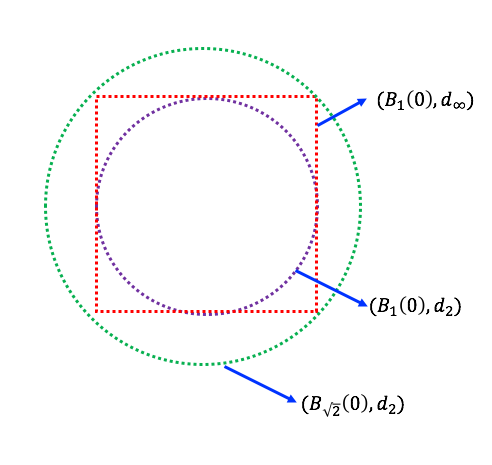
\includegraphics[width=8cm]{week1/f_3_3}
\caption{The diagram for the relation $(B_1(x),d_2)\subseteq(B_\infty(x),d_\infty)\subseteq (B_{\sqrt{2}}(x),d_2)$ on $\mathbb{R}^2$}
\end{figure}
It's easy to conclude the simple generalization for example~(\ref{Exp:1:16}):
\begin{proposition}
If $d$ and $\rho$ are equivalent, then 
\[
\lim_{n\to\infty}d(x_n,x)=0\Longleftrightarrow
\lim_{n\to\infty}\rho(x_n,x)=0
\]
\end{proposition}
Note that this does not necessarily hold for topology spaces.
\item
Consider $d_1,d_\infty$ in $\mathcal{C}[a,b]$:
\[
d_1(f,g):=\int_a^b|f-g|\diff x\le
\int_a^b\sup_{[a,b]}|f-g|\diff x=(b-a)d_\infty(f,g),
\]
i.e., $d_\infty$ is stronger than $d_1$. Question: Are they equivalent? \emph{No}.
\begin{proof}[Justification]
Consider $f_n(x)=n^2x^n(1-x)$ for $x\in[0,1]$. Check that
\[
\lim_{n\to\infty}d_1(f_n(x),0)=0,\quad
\mbox{but }d_\infty(f_n(x),0)\to\infty
\]
The peak of $f_n$ may go to infinite, while the integration converges to zero, i.e., there is no $K>0$ such that $d_{\infty}(f_n,0) < K d_1(f_n,0),\forall n\in\mathbb{N}$.
\end{proof}
We will discuss this topic at Lebsegue integration again.
\end{enumerate}
\end{example}
\subsection{Continuity}
\begin{definition}[Continuity]
Let $f:(X,d)\to(Y,d)$ be a function and $x_0\in X$. Then $f$ is continuous at $x_0$ if 
$\forall\varepsilon>0$, there exists $\delta>0$ such that
\[
d(x,x_0)<\delta\implies
\rho(f(x),f(x_0))<\varepsilon
\]
The function $f$ is continuous in $X$ if $f$ is continuous for all $x_0\in X$.
\end{definition}
\begin{proposition}\label{Pro:1:12}
The function $f$ is continuous at $x$ if and only if for all $\{x_n\}\to x$ under $d$, $f(x_n)\to f(x)$ under $\rho$.
\end{proposition}
\begin{proof}
\textit{Necessity:}
Given $\varepsilon>0$, by continuity, 
\begin{equation}\label{Eq:1:3}
d(x,x')<\delta\implies \rho(f(x'),f(x))<\varepsilon.
\end{equation}
Consider the sequence $\{x_n\}\to x$, then there exists $N$ such that $d(x_n,x)<\delta$ for $\forall n\ge N$. By applying (\ref{Eq:1:3}), $\rho(f(x_n),f(x))<\varepsilon$ for $\forall n\ge N$, i.e., $f(x_n)\to f(x)$.

\textit{Sufficiency}:
Assume that $f$ is not continuous at $x$, then there exists $\varepsilon_0$ such that for $\delta_n=\frac{1}{n}$, there exists $x_n$ such that
\[
d(x_n,x)<\delta_n,\mbox{ but }\rho(f(x_n),f(x))>\varepsilon_0.
\]
Then $\{x_n\}\to x$ by our construction, while $\{f(x_n)\}$ does not converge to $f(x)$, which is a contradiction.
\end{proof}
\begin{corollary}
If the function $f:(X,d)\to(Y,\rho)$ is continuous at $x$, the function $g:(Y,\rho)\to(Z,m)$ is continuous at $f(x)$,
then $g\circ f:(X,d)\to(Z,m)$ is continuous at $x$.
\end{corollary}
\begin{proof}
Note that
\[
\{x_n\}\to x
\xLongrightarrow{(a)}
\{f(x_n)\}\to f(x)
\xLongrightarrow{(b)}
\{g(f(x_n))\}\to g(f(x))
\xLongrightarrow{(c)}
g\circ f\mbox{ is continuous at $x$}.
\]
where $(a),(b),(c)$ are all by proposition~(\ref{Pro:1:12}).
\end{proof}
\subsection{Open and Closed Sets}
We have open/closed intervals in $\mathbb{R}$, and they are important in some theorems (e.g, continuous functions bring closed intervals to closed intervals).
\begin{definition}[Open]
Let $(X,d)$ be a metric space.  A set $U\subseteq X$ is open if for each $x\in U$, there exists $\rho_x>0$ such that $B_{\rho_x}(x)\subseteq U$. The empty set $\emptyset$ is defined to be open.
\end{definition}
\begin{example}
Let $(\mathbb{R},d_2\mbox{ or }d_\infty)$ be a metric space. The set $U=(a,b)$ is open.
\end{example}
\begin{proposition}
\begin{enumerate}
\item
Let $(X,d)$ be a metric space. Then all open balls $B_r(x)$ are open
\item
All open sets in $X$ can be written as a union of open balls.
\end{enumerate}
\end{proposition}
\begin{proof}
\begin{enumerate}
\item
Let $y\in B_r(x)$, i.e., $d(x,y):=q<r$. Consider the open ball $B_{(r-q)/2}(y)$. It suffices to show $B_{(r-q)/2}(y)\subseteq B_r(x)$. For any $z\in B_{(r-q)/2}(y)$,
\[
d(x,z)\le d(x,y)+d(y,z)<q+\frac{r-q}{2}=\frac{r+q}{2}<r.
\]
The proof is complete.
\item
Let $U\subseteq X$ be open, i.e., for $\forall x\in U$, there exists $\varepsilon_x>0$ such that $B_{\varepsilon_x}(x)\subseteq U$. Therefore
\[
\{x\}\subseteq B_{\varepsilon_x}(x)\subseteq U,\forall x\in U
\]
which implies
\[
U=\bigcup_{x\in U}\{x\}\subseteq \bigcup_{x\in U}B_{\varepsilon_x}(x)\subseteq U,
\]
i.e., $U=\bigcup_{x\in U}B_{\varepsilon_x}(x)$.
\end{enumerate}
\end{proof}

















\section{Wednesday for MAT4002}\index{Monday_lecture}
\subsection{Remarks on product space} 
\paragraph{Reviewing}
\begin{itemize}
\item
Product Topology: For topological space $(X,\mathcal{T}_X)$ and $(Y,\mathcal{Y})$, define the basis
\[
\mathcal{B}_{X\times Y}=\{U\times V\mid U\in\mathcal{T}_X,V\in\mathcal{T}_Y\}
\]
and the family of union of subsets in $\mathcal{B}_{X\times Y}$ forms a product topology.
\end{itemize}
\begin{proposition}
a ring torus is homeomorphic to the Cartesian product of two circles, say $S^1\times S^1\cong T$.
\end{proposition}
 \begin{proof}
 Define a mapping $f:[0,2\pi]\times [0,2\pi]\to T$ as
 \[
 f(\theta,\phi)=\begin{pmatrix}
(R+r\cos\theta)\cos\phi,
&
(R+r\cos\theta)\sin\phi,
&
r\sin\theta
\end{pmatrix}
 \]
Define $i:T\to\mathbb{R}^3$, we imply
 \[
 i\circ f:[0,2\pi]\times[0,2\pi]\to\mathbb{R}^3\ \text{is continuous}
 \]
 Therefore we imply $f:[0,2\pi]\times [0,2\pi]\to T$ is continuous. Together with the condition that 
\[
\left\{
\begin{aligned}
f(0,y)&=f(2\pi,y)\\
f(x,0)&=f(x,2\pi)
\end{aligned}
\right.
\]
we imply the function $f:S^1\times S^1\to T$ is continuous.
We can also show it is bijective. We can also show $f^{-1}$ is continuous.
 \end{proof}
 
\begin{proposition}
\begin{enumerate}
\item
Let $X\times Y$ be endowed with product topology. 
The projection mappings defined as
\begin{align*}
p_X:&X\times Y\to X,\ \text{with }p_X(x,y) = x\\
p_Y:&X\times Y\to Y,\ \text{with }p_Y(x,y)=y
\end{align*}
are continuous.
\item
(an equivalent definition for product topology)
The product topology is the \emph{coarest topology} on $X\times Y$ such that $p_X$ and $p_Y$ are both continuous.
\item
(an equivalent definition for product topology)
Let $Z$ be a topological space, then the product topology is the unique topology that the red and the blue line in the diagram commutes:
\begin{figure}[H]
\centering
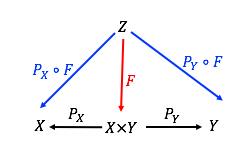
\includegraphics[width=6cm]{week3/p_3}
\caption{Diagram summarizing the statement~(*)}
\end{figure}
namely,
\begin{quotation}
\textit{
the mapping $F:Z\to X\times Y$ is continuous iff both $P_X\circ F:Z\to X$ and $P_Y\circ F:Z\to Y$ are continuous}. (*)
\end{quotation}
\end{enumerate}
\end{proposition}
\begin{proof}
\begin{enumerate}
\item
For any open $U$, we imply $p_X^{-1}(U)=U\times Y\in\mathcal{B}_{X\times Y}\subseteq\mathcal{T}_{X\times Y}$, i.e., $p_X^{-1}(U)$ is open. The same goes for $p_Y$.
\item
It suffices to show any topology $\mathcal{T}$ that meets the condition in (2) must contain $\mathcal{T}_{\text{product}}$. We imply that for $\forall U\in\mathcal{T}_X,V\in\mathcal{T}_Y$, 
\[
\left\{
\begin{aligned}
p_X^{-1}(U)&=U\times X\in\mathcal{T}\\
p_Y^{-1}(V)&=X\times V\in\mathcal{T}
\end{aligned}
\right.
\implies
(U\times Y)\cap(X\times V)=(U\cap X)\times (Y\cap V)=U\times V\in\mathcal{T},
\]
which implies $\mathcal{B}_{X\times Y}\subseteq\mathcal{T}$. Since $\mathcal{T}$ is closed for union operation on subsets, we imply $\mathcal{T}_{\text{product topology}}\subseteq\mathcal{T}$.
\item
\begin{enumerate}
\item
Firstly show that $\mathcal{T}_{\text{product}}$ satisfies (*).
\begin{itemize}
\item
For the forward direction, by (1) we imply both $p_X\circ F$ and $p_Y\circ F$ are continuous, since the composition of continuous functions are continuous as well.
\item
For the reverse direction, for $\forall U\times\mathcal{T}_X,V\in\mathcal{T}_Y$,
\[
F^{-1}(U\times V)=(p_X\circ F)^{-1}(X)\cap (p_Y\circ F)^{-1}(Y),
\]
which is open due to the continuity of $p_X\circ F$ and $p_Y\circ F$.
\end{itemize}
\item
Then we show the uniqueness of $\mathcal{T}_{\text{product}}$. Let $\mathcal{T}$ be another topology $X\times Y$ satisfying (*).
\begin{itemize}
\item
Take $Z=(X\times Y,\mathcal{T})$, and consider the identity mapping $F=\text{id}:Z\to Z$, which is continuous. Therefore $p_X\circ\text{id}$ and $p_Y\circ\text{id}$ are continuous, i.e., $p_X$ and $p_Y$ are continuous. By (2) we imply $\mathcal{T}_{\text{product}}\subseteq\mathcal{T}$.
\item
Take $Z=(X\times Y,\mathcal{T}_{\text{product}})$, and consider the identity mapping $F=\text{id}:Z\to Z$. Note that $p_X\circ F=p_X$ and $p_Y\circ F=p_Y$, which is continuous by (1). Therefore, the identity mapping $F:(X\times Y,\mathcal{T}_{\text{product}})\to(X\times Y,\mathcal{T})$ is continuous, which implies
\[
U=\text{id}^{-1}(U)\subseteq\mathcal{T}_{\text{product}}\ \text{for }\forall U\in\mathcal{T},
\]
i.e., $\mathcal{T}\subseteq\mathcal{T}_{\text{product}}.$
\end{itemize}
The proof is complete.
\end{enumerate}


\end{enumerate}
\end{proof}

\begin{definition}[Disjoint Union]
Let $X\times Y$ be two topological spaces, then the \emph{disjoint union} of $X$ and $Y$ is
\[
X\coprod Y:=(X\times\{0\})\cup(Y\times\{1\})
\]
\end{definition}
\begin{remark}
\begin{enumerate}
\item
We define that $U$ is open in $X\coprod Y$ if
\begin{enumerate}
\item
$U\cap(X\times\{0\})$ is open in $X\times\{0\}$; and
\item
$U\cap(Y\times\{1\})$ is open in $Y\times\{1\}$.
\end{enumerate}
We also need to show the well-definedness for this definition.
\item
$S$ is open in $X\coprod Y$ iff $S$ can be expressed as
\[
S=(U\times\{0\})\cup(V\times\{1\})
\]
where $U\subseteq X$ is open and $V\subseteq Y$ is open.
\end{enumerate}
\end{remark}


\subsection{Properties of Topological Spaces}
\subsubsection{Hausdorff Property}
\begin{definition}[First Separation Axiom]
A topological space $X$ satisfies the \emph{first separation axiom} if for any two distinct points $x\ne y\in X$, there exists open $U\ni x$ but not including $y$.
\end{definition}

\begin{proposition}
A topological space $X$ has first separation property if and only if for $\forall x\in X$, $\{x\}$ is closed in $X$.
\end{proposition}
\begin{proof}
\textit{Sufficiency.}
Suppose that $x\ne y$, then construct $U:=X\setminus\{y\}$, which is a open set that contains $x$ but not includes $y$.

\textit{Necessity.}
Take any $x\in X$, then for $\forall y\ne x$, there exists $y\in U_y$ that is open and $x\notin U_y$. Thus 
\[
\{y\}\subseteq U_y\subseteq X\setminus\{x\}
\]
which implies
\[
\bigcup_{y\in X\setminus\{x\}}\{y\}\subseteq
\bigcup_{y\in X\setminus\{x\}}U_y\subseteq
X\setminus\{x\},
\]
i.e., $X\setminus\{x\}=\bigcup_{y\in X\setminus\{x\}}U_y$ is open in $X$, i.e., $\{x\}$ is closed in $X.$
\end{proof}

\begin{definition}[Second separation Axiom]
A topological space satisfies the \emph{second separation axiom} (or $X$ is Hausdorff) if for all $x\ne y$ in $X$, there exists open sets $U,V$ such that
\[
\begin{array}{lll}
x\in U,
&
y\in V,
&
U\cap V=\emptyset
\end{array}
\]
\end{definition}

\begin{example}
All metrizable topological spaces are Hausdorff.

Suppose $d(x,y)=r>0$, then take $B_{r/2}(x)$ and $B_{r/2}(y)$
\end{example}

\begin{example}
Note that a topological space that is \emph{first separable} may not necessarily be \emph{second separable}:

Consider $\mathcal{T}_{\text{co-finite}}$, then $X$ is first separable but not Hausdorff:

Suppose on the contrary that for given $x\ne y$, there exists open sets $U,V$ such that $x\in U,y\in V$, and
\[
U\cap V=\emptyset\implies
X = X\setminus (U\cap V) = (X\setminus U)\cup(X\setminus V),
\]
implying that the union of two finite sets equals $X$, which is infinite, which is a contradiction.
\end{example}



















\chapter{Week4}
\section{Monday for MAT3040}\index{Monday_lecture}

\subsection{Quotient Spaces}

Now we aim to divide a big \emph{vector space} into many pieces of slices. 
\begin{itemize}
\item
For example, the Cartesian plane can be expressed as union of set of vertical lines as follows:
\[
\mathbb{R}^2 = \bigcup_{m\in\mathbb{R}}\left\{\begin{pmatrix}
m\\0
\end{pmatrix}+
\Span\{(0,1)\}\}
\right\}
\]
\item
Another example is that the set of integers can be expressed as union of three sets:
\[
\mathbb{Z}
=
Z_1\cup Z_2\cup Z_3,
\]
where $Z_i$ is the set of integers $z$ such that $z\text{ mod }3 = i$.
\end{itemize}

\begin{definition}[Coset]
Let $V$ be a vector space and $W\le V$. For any element $\bm v\in V$, the \emph{(right) coset} determined by $\bm v$ is the set
\[
\bm v+W:=\{\bm v+\bm w\mid\bm w\in W\}
\]
\end{definition}

For example, consider $V=\mathbb{R}^3$ and $W=\Span\{(1,2,0)\}$. Then the coset determined by $\bm v=(5,6,-3)$ can be written as
\[
\bm v+W=\left\{(5+t,6+2t,-3)\mid t\in\mathbb{R}\right\}
\]
It's interesting that the coset determined by $\bm v'=\{(4,4,-3)\}$ is exactly the same as the coset shown above:
\[
\bm v'+W=\left\{(4+t,4+2t,-3)\mid t\in\mathbb{R}\right\}=\bm v+W.
\]

Therefore, write the exact expression of $\bm v+W$ may sometimes become tedious and hard to check the equivalence. We say $\bm v$ is a \emph{representative} of a coset $\bm v+W$.

\begin{proposition}\label{pro:4:1}
Two cosets are the same iff the subtraction for the corresponding representatives is in $W$, i.e., 
\[
\bm v_1+W=\bm v_2+W
\Longleftrightarrow
\bm v_1-\bm v_2\in W
\]
\end{proposition}
\begin{proof}
\textit{Necessity.}
Suppose that $\bm v_1+W=\bm v_2+W$, then $\bm v_1+\bm w_1=\bm v_2+\bm w_2$ for some $\bm w_1,\bm w_2\in W$, which implies
\[
\bm v_1-\bm v_2=\bm w_2-\bm w_1\in W
\]
\textit{Sufficiency.}
Suppose that $\bm v_1-\bm v_2=\bm w\in W$. It suffices to show $\bm v_1+W\subseteq\bm v_2+W$.
For any $\bm v_1+\bm w'\in \bm v_1+W$, this element can be expressed as
\[
\bm v_1+\bm w'=(\bm v_2+\bm w)+\bm w'=\bm v_2+\underbrace{(\bm w+\bm w')}_{\text{belong to $W$}}\in \bm v_2+W.
\]
Therefore, $\bm v_1+W\subseteq \bm v_2+W$. Similarly we can show that $\bm v_2+W\subseteq \bm v_1+W$.
\end{proof}
\textit{Exercise: }Two cosets with representatives $\bm v_1,\bm v_2$ have no intersection iff $\bm v_1-\bm v_2\notin W$.

\begin{definition}[Quotient Space]
The \emph{quotient space} of $V$ by the subspace $W$, is the collection of all cosets $\bm v+W$, denoted by $V/ W$.
\end{definition}
To make the quotient space a vector space structure, we define the addition and scalar multiplication on $V/ W$ by:
\begin{align*}
(\bm v_1+W)+(\bm v_2+W)&:=(\bm v_1+\bm v_2)+W\\
\alpha\cdot (\bm v+W)&:=(\alpha\cdot\bm v) + W
\end{align*}

For example, consider $V=\mathbb{R}^2$ and $W=\Span\{(0,1)\}$. Then note that
\begin{align*}
\left(
\begin{pmatrix}
1\\0
\end{pmatrix}+W
\right)
+
\left(
\begin{pmatrix}
2\\0
\end{pmatrix}+W
\right)
&=
\left(
\begin{pmatrix}
3\\0
\end{pmatrix}+W
\right)\\
\pi\cdot\left(
\begin{pmatrix}
1\\0
\end{pmatrix}+W
\right)
&=
\left(
\begin{pmatrix}
\pi\\0
\end{pmatrix}+W
\right)
\end{align*}

\begin{proposition}
The addition and scalar multiplication is well-defined.
\end{proposition}
\begin{proof}
\begin{enumerate}
\item
Suppose that
\begin{equation}\label{Eq:4:1}
\left\{
\begin{aligned}
\bm v_1+W&=\bm v_1'+W\\
\bm v_2+W&=\bm v_2'+W
\end{aligned}
\right.,
\end{equation}
and we need to show that $(\bm v_1+\bm v_2)+W=(\bm v_1'+\bm v_2')+W$. 

From (\ref{Eq:4:1}) and proposition~(\ref{pro:4:1}), we imply
\[
\bm v_1-\bm v_1'\in W,\quad
\bm v_2-\bm v_2'\in W
\]
which implies
\[
(\bm v_1-\bm v_1')+(\bm v_2-\bm v_2')=(\bm v_1+\bm v_2) - (\bm v_1'+\bm v_2')\in W
\]

By proposition~(\ref{pro:4:1}) again we imply $(\bm v_1+\bm v_2)+W=(\bm v_1'+\bm v_2')+W$
\item
For scalar multiplication, similarly, we can show that $\bm v_1+W=\bm v_1'+W$ implies $\alpha\bm v_1+W=\alpha\bm v_1'+W$ for all $\alpha\in\mathbb{F}$.

\end{enumerate}

\end{proof}

\begin{proposition}
The canonical projection mapping
\[
\begin{aligned}
\pi_W:&V\to V/ W,\\
&\bm v\mapsto\bm v+W,
\end{aligned}
\]
is a \emph{surjective} \emph{linear transformation} with $\ker(\pi_W) = W$.
\end{proposition}
\begin{proof}
\begin{enumerate}
\item
First we show that $\ker(\pi_W)=W$:
\[
\pi_W(\bm v)=0\implies
\bm v+W=\bm0_{V/ W}\implies
\bm v+W=\bm0+W\implies \bm v=(\bm v-\bm0)\in W
\]
Here note that the zero element in the quotient space $V/ W$ is the coset with representative $\bm0$.
\item
For any $\bm v_0+W\in V/ W$, we can construct $\bm v_0\in V$ such that $\pi_W(\bm v_0)=\bm v_0+W$. Therefore the mapping $\pi_W$ is surjective.
\item
To show the mapping $\pi_W$ is a linear transformation, note that
\begin{align*}
\pi_W(\alpha\bm v_1+\beta\bm v_2)&=(\alpha\bm v_1+\beta\bm v_2)+W\\
&=(\alpha\bm v_1+W)+(\beta\bm v_2+W)\\
&=\alpha(\bm v_1+W)+\beta(\bm v_2+W)\\
&=\alpha\pi_W(\bm v_1)+\beta\pi_W(\bm v_2)
\end{align*}

\end{enumerate}


\end{proof}



\subsection{First Isomorphism Theorem}
The key of linear algebra is to solve the linear system $\bm A\bm x=\bm b$ with $\bm A\in\mathbb{R}^{m\times n}$. 
The general step for solving this linear system is as follows:
\begin{enumerate}
\item
Find the solution set for $\bm A\bm x=\bm0$, i.e., the set $\ker(\bm A)$
\item
Find a particular solution $\bm x_0$ such that $\bm A\bm x_0=\bm b$.
\end{enumerate}
Then the general solution set to this linear system is $\bm x_0+\ker(\bm A)$, which is a coset in the space $\mathbb{R}^n/ \ker(\bm A)$. Therefore, to solve the linear system $\bm{Ax}=\bm b$ suffices to study the quotient space $\mathbb{R}^n/ \ker(\bm A)$:

\begin{proposition}[Universal Property I]
Suppose that $T:V\to W$ is a linear transformation, and that $V'\le\ker(T)$. Then the mapping
\begin{align*}
\tilde{T}&:V/ V'\to W\\
&\bm v+V'\mapsto T(\bm v)
\end{align*}
is a well-defined linear transformation. As a result, the diagram below commutes:
\begin{figure}[H]
\centering
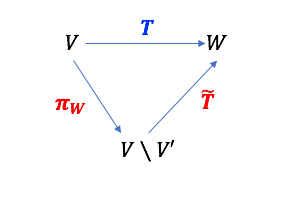
\includegraphics[width=0.5\textwidth]{week4/p_1}
\end{figure}
In other words, we have $T = \tilde{T}\circ \pi_W$.
\end{proposition}

\begin{proof}
First we show the well-definedness. Suppose that $\bm v_1+V'=\bm v_2+V'$ and suffices to show $\tilde T(\bm v_1+V')=\tilde T(\bm v_2+V')$, i.e., $T(\bm v_1)=T(\bm v_2)$. By proposition~(\ref{pro:4:1}), we imply
\[
\bm v_1-\bm v_2\in V'\le\ker(T)\implies
T(\bm v_1-\bm v_2)=\bm0\implies T(\bm v_1)-T(\bm v_2)=\bm0.
\]
Then we show $\tilde(T)$ is a linear transformation:
\begin{align*}
\tilde{T}(\alpha(\bm v_1+V')  + \beta(\bm v_2+V'))&=\tilde{T}((\alpha\bm v_1+\beta\bm v_2)+V')\\
&=T(\alpha\bm v_1+\beta\bm v_2)\\
&=\alpha T(\bm v_1)+\beta T(\bm v_2)\\
&=\alpha\tilde{T}(\bm v_1+V')+\beta\tilde{T}(\bm v_2+V')
\end{align*}
\end{proof}

Actually, if we let $V'=\ker(T)$, the mapping $\tilde{T}:V/ V'\to T(V)$ forms an isomorphism, In particular, if further $T$ is surjective, then $T(V)=W$, i.e., the mapping $\tilde{T}:V/ V'\to W$ forms an isomorphism.
\begin{theorem}[First Isomorphism Theorem]
Let $T:V\to W$ be a surjective linear transformation. Then the mapping 
\begin{align*}
\tilde{T}&:V/ \ker(T)\to W\\
&\bm v+\ker(T)\mapsto T(\bm v)
\end{align*}
is an isomorphism.
\end{theorem}
\begin{proof}
\textit{Injectivity.} Suppose that $\tilde{T}(\bm v_1+\ker(T)) = \tilde{T}(\bm v_2+\ker(T))$, then we imply
\[
T(\bm v_1)=T(\bm v_2)\implies T(\bm v_1-\bm v_2)=\bm0_W\implies\bm v_1-\bm v_2\in\ker(T),
\]
i.e., $\bm v_1+\ker(T)=\bm v_2+\ker(T)$.

\textit{Surjectivity.} For $\bm w\in W$, due to the surjectivity of $T$, we can find a $\bm v_0$ such that $T(\bm v_0)=\bm w$. Therefore, we can construct a set $\bm v_0+\ker(T)$ such that
\[
\tilde{T}(\bm v_0+\ker(T))=\bm w.
\]
\end{proof}




















\section{Monday for MAT3006}\index{Monday_lecture}
\subsection{Remarks on MCT}
\begin{example}
The MCT can help us to compute the integral
\begin{align*}
\lim_{n\to\infty}\int_{[0,n\pi]}\cos\left(\frac{x}{2n}\right)xe^{-x^2}\diff x
\end{align*}

Construct $f_n(x) = \cos\left(\frac{x}{2n}\right)xe^{-x^2}\mathcal{X}_{[0,n\pi]}$.
\begin{itemize}
\item
Since $\cos(x/2n)<\cos(x/2(n+1))$ for any $x\in[0,n\pi]$, we imply $f_n$ is monotone increasing with $n$
\item
$f_n(x)$ is integrable for all $n$.
\item
$f_n$ converges pointwise to $xe^{-x^2}\mathcal{X}_{[0,\infty)}$
\end{itemize}
Therefore, MCT I applies and
\[
\lim_{n\to\infty}\int_{[0,n\pi]}\cos\left(\frac{x}{2n}\right)xe^{-x^2}\diff x
=
\int\left(\lim_{n\to\infty}f_n\right)\diff m
\]
with
\[
\lim_{n\to\infty}f_n = xe^{-x^2}\mathcal{X}_{[0,\infty)}.
\]
Moreover, 
\begin{subequations}
\begin{align}
\int\left(\lim_{n\to\infty}f_n\right)\diff m &= 
\lim_{m\to\infty}\int_{[0,m]}xe^{-x^2}\diff x\label{Eq:12:1}\\
&=\int_0^\infty xe^{-x^2}\diff x\\
&=\frac{1}{2}
\end{align}
where (\ref{Eq:12:1}) is by applying MCT I with $g_m(x) = xe^{-x^2}\mathcal{X}_{[0,m]}$ and proposition~(\ref{pro:10:14}) to compute a Lebesgue integral by evaluating a proper Riemann integral.
\end{subequations}
\end{example}

Then we discuss the Lebesgue integral for series:

\begin{corollary}[Lebesgue Series Theorem]
Let $\{f_n\}$ be a series of measurable functions such that
\[
\sum_{n=1}^\infty\int|f_n|\diff m<\infty,
\]
then $\sum_{n=1}^kf_n$ converges to an integrable function $f = \sum_{n=1}^\infty f_n$ a.e., with
\[
\int f\diff m = \sum_{n=1}^\infty\int f_n\diff m
\]
\end{corollary}
\begin{proof}
\begin{itemize}
\item
For each $f_n$, consider 
\[
f_n = f_n^+ - f_n^-,\ \text{where $f_n^+,f_n^-$ are nonnegative}.
\]
By proposition~(\ref{pro:11:6}), 
\[
\int\sum_{n=1}^\infty f_n^+\diff m = \sum_{n=1}^\infty\int f_n^+\diff m\le \sum_{n=1}^\infty\int |f_n|\diff m<\infty.
\]
Therefore, $f^+:=\sum_{n=1}^\infty f_n^+=\lim_{k\to\infty}\sum_{n=1}^kf_n^+$ is integrable.
The same follows by replacing $f^{+}$ with $f^{-}$.
By corollary~(\ref{cor:9:6}), $f^+(x),f^-(x)<\infty,\forall x\in U$, where $U^c$ is null.
\item
Therefore, construct 
\[
f(x)=\left\{
\begin{aligned}
f^+(x)-f^-(x),&\quad x\in U\\
0,&\quad x\in U^c
\end{aligned}
\right.
\]
Moreover, for $x\in U$, 
\begin{align*}
f(x)&=\left(\lim_{k\to\infty}\sum_{n=1}^kf_n^+(x)\right)-
\left(\lim_{k\to\infty}\sum_{n=1}^kf_n^-(x)\right)\\
&=\lim_{k\to\infty}
\left(
\sum_{n=1}^kf_n^+(x)
-
\sum_{n=1}^kf_n^-(x)
\right)\\
&=\lim_{k\to\infty}\left[\sum_{n=1}^k(f_n^+(x)-f_n^-(x))\right]
\\&=
\sum_{n=1}^\infty f_n(x)
\end{align*}
where the first equality is because that both terms are finite.
\item
It follows that
\begin{subequations}
\begin{align}
\int f\diff m&=\int f^+\diff m - \int f^-\diff m\label{Eq:12:2:a}\\
&=
\int\sum_{n=1}^\infty f_n^+\diff m -\int\sum_{n=1}^\infty f_n^-\diff m\\
&=\left(\sum_{n=1}^\infty\int f_n^+\diff m\right)
-
\left(\sum_{n=1}^\infty\int f_n^-\diff m\right)\label{Eq:12:2:c}\\
&=\sum_{n=1}^\infty
\left(
\int f_n^+\diff m -\int f_n^-\diff m
\right)\label{Eq:12:2:d}\\
&=\sum_{n=1}^\infty\int f_n\diff m\label{Eq:12:2:e}
\end{align}
where (\ref{Eq:12:2:a}),(\ref{Eq:12:2:d}) is because that summation/subtraction between series holds when these series are finite; (\ref{Eq:12:2:c}) is by proposition~(\ref{pro:11:6}); (\ref{Eq:12:2:e}) is by definition of $f_n$.
\end{subequations}
\end{itemize}
\end{proof}

\begin{example}
Compute the integral
\[
\int_{(0,1]}e^{-x}x^{\alpha-1}\diff x,\ \alpha>0.
\]
\begin{itemize}
\item
Construct $f_n(x) = (-1)^n\frac{x^{\alpha+n-1}}{n!}\mathcal{X}_{(0,1]}, n\ge0$, and
\[
\sum_{n=0}^N f_n(x)\to e^{-x}x^{\alpha-1}, \ \text{pointwisely}, x\in(0,1]. 
\]
By applying MCT I,
\[
\int|f_n|\diff m=\frac{1}{(\alpha+n)n!}
\]
Therefore, 
\[
\sum_{n=0}^\infty\int|f_n|\diff m=
\sum_{n=0}^\infty\frac{1}{(\alpha+n)n!}<\infty
\]
\item
Applying the Lebesgue Series Theorem,
\[
\int_{(0,1]}e^{-x}x^{\alpha-1}\diff x = 
\int_{(0,1]}(\sum_{n=0}^\infty f_n)\diff m
=
\sum_{n=0}^\infty\int f_n\diff m=
\sum_{n=0}^\infty\frac{(-1)^n}{(\alpha+n)n!}
\]
\end{itemize}
\end{example}

\begin{remark}
It's essential to have $\sum\int|f|\diff m<\infty$ rather than $\sum\int f_n\diff m<\infty$ in the Lebesgue Series Theorem.
For example, let
\[
f_n=\frac{(-1)^{n+1}}{(n+1)}\mathcal{X}_{[n,n+1)}
\implies
\sum_{n=1}^\infty\int f_n\diff m =\log(2)<\infty
\]
However, $f:=\sum f_n$ is not integrable.
\end{remark}

\subsection{Dominated Convergence Theorem}
\begin{theorem}
Let $\{f_n\}$ be a sequence of measruable functions such that $|f_n|\le g$ a.e., and $g$ is integrable.
Suppose that $\lim_{n\to\infty}f_n(x)=f(x)$ a.e., then
\begin{enumerate}
\item
$f$ is integrable,
\item
\[
\int f\diff m =\lim_{n\to\infty}\int f_n\diff m
\]
\end{enumerate}
\end{theorem}
\begin{proof}
\begin{itemize}
\item
Observe that 
\[
|f_n|\le g\implies
\lim_{n\to\infty}|f_n|\le g\implies |f|\le g
\]
By comparison test, $g$ is integrable implies $|f|$ is integrable, and further $f$ is integrable.
\item
Consider the sequence of non-negative functions
$\{g-f_n\}_{n\in\mathbb{N}}$ and $\{g+f_n\}_{n\in\mathbb{N}}$.

By Fatou's Lemma, 
\begin{align*}
\lim_{n\to\infty}\inf\int(g-f_n)\diff m&\ge \int \lim_{n\to\infty}\inf(g-f_n)\diff m\\
&=\int(g-f)\diff m\\
&=\int g\diff m - \int f\diff m
\end{align*}
which follows that
\[
\int g\diff m - \lim_{n\to\infty}\sup\int f_n\diff m
\ge
\int g\diff m - \int f\diff m
\]
i.e.,
\[
\int f\diff m\ge  \lim_{n\to\infty}\sup\int f_n\diff m
\]
\item
Similarly, 
\[
\lim_{n\to\infty}\inf(g+f_n)\diff m\ge \int\lim_{n\to\infty}\inf(g+f_n)\diff m
=
\int g\diff m + \int f\diff m
\]
which implies
\[
 \lim_{n\to\infty}\inf\int f_n\diff m\ge\int f\diff m
\]
\end{itemize}
As a result,
\[
 \lim_{n\to\infty}\sup\int f_n\diff m
 \le
 \int f\diff m\le  \lim_{n\to\infty}\inf\int f_n\diff m,
\]
which implies
\[
\int f\diff m = \lim_n\int f_n\diff m
\]
\end{proof}

\begin{corollary}[Bounded Convergence Theorem]
Suppose that $E\in\mathcal{M}$ be such that $m(E)<\infty$.
If
\begin{itemize}
\item
$|f_n(x)|\le K<\infty$ for any $x\in E,n\in\mathbb{N}$
\item
$f_n\to f$ a.e. in $E$,
\end{itemize}
then $f$ is integrable in $E$ with
\[
\int_Ef\diff m = \lim_{n\to\infty}\int f_n\diff m
\]
\end{corollary}
\begin{proof}
Take $g=K\mathcal{X}_E$ in DCT.
\end{proof}


\begin{proposition}
Every Riemann integrable function $f$ on $[a,b]$ is Lebesgue integrable, without the condition that $f$ is continuous a.e.
\end{proposition}
\begin{proof}
Since $f$ is Riemann integrable, we imply $f$ is bounded.
We construct the Riemann lower abd upper functions with $2^n$ equal intervals, denoted as $\{\phi_n\}$ and $\{\psi_n\}$, which follows that
\begin{itemize}
\item
$\phi_n$ is monotone increasing;
$\psi_n$ is monotone decreasing;
\item
$\phi_n\le f\le \psi_n$, and
\[
\lim_{n\to\infty}\int_{[a,b]}\phi_n=\int_a^bf(x)\diff x = \lim_{n\to\infty}\int_{[a,b]}\psi_n.
\]
\end{itemize}
Construct $g=\sup_n\phi_n$ and $h=\inf_n\psi_n$.
Now we can apply the bounded convergence theorem:
\begin{itemize}
\item
$\phi_n$ is bounded on $[a,b]$
\item
$\phi_n\to g$ on $[a,b]$
\end{itemize}
which implies
$g$ is Lebesgue integrable on $[a,b]$, with 
\[
\int_{[a,b]}g\diff m = \lim_{n\to\infty}\int_{[a,b]}\phi_n\diff m=\int_a^bf(x)\diff x.
\]
Similarly, $h$ is Lebesgue integrable, with
\[
\int_{[a,b]}h\diff m = \lim_{n\to\infty}\int_{[a,b]}\psi_n\diff m=\int_a^bf(x)\diff x.
\]
Moreover, $g\le f\le h$, and
\[
\int_{[a,b]}(h-g)\diff m = \int_{[a,b]}h\diff m - \int_{[a,b]}g\diff m=\int_a^bf(x)\diff x-\int_a^bf(x)\diff x=0,
\]
which implies $h=g$ a.e., and further $f=g$ a.e., which implies
\[
\int_{[a,b]} f\diff m = \int_{[a,b]} g\diff m= \int_a^bf(x)\diff x.
\]
\end{proof}
\begin{remark}
However, an improper Riemann integral does not necessarily has the corresponding Lebesgue integral:
\[
f(x)=\sum_{n=1}^\infty (-1)^nn\cdot\mathcal{X}_{(1/(n+1),1/n]},\ x\in[0,1]
\]
In this case, $f$ is Riemann integrable but not Lebesgue integrable.
\end{remark}














\section{Monday for MAT4002}\index{Monday_lecture}

\paragraph{Reviewing}
\begin{enumerate}
\item
Topological Space $(X,\mathcal{J})$: a special class of topological space is that induced from metric space $(X,d)$:
\[
(X,\mathcal{T}),\quad\text{with }\mathcal{T}=\{\text{all open sets in $(X,d)$}\}
\]
\item
Closed Sets $(X\setminus U)$ with $U$ open.
\end{enumerate}

\begin{proposition}
Let $(X,\mathcal{T})$ be a topological space, 
\begin{enumerate}
\item
$\emptyset, X$ are closed in $X$
\item
$V_1,V_2$ closed in $X$ implies that $V_1\bigcup V_2$ closed in $X$
\item
$\{V_\alpha\mid\alpha\in\mathcal{A}\}$ closed in $X$ implies that $\bigcap_{\alpha\in\mathcal{A}}V_\alpha$ closed in $X$
\end{enumerate}
\end{proposition}
\begin{proof}
Applying the De Morgan's Law
\[
(X\setminus\bigcup_{i\in I}U_i)=\bigcap_{i\in I}(X\setminus U_i)
\]
\end{proof}

\subsection{Convergence in topological space}

\begin{definition}[Convergence]
A sequence $\{x_n\}$ of a topological space $(X,\mathcal{T})$ converges to $x\in X$ 
if $\forall U\ni x$ is open, there $\exists N$ such that $x_n\in U,\forall n\ge N$.
\end{definition}

\begin{example}
\begin{enumerate}
\item
The topology for the space $(X=\mathbb{R}^n,d_2)\to(X,\mathcal{T})$ (i.e., a topological space induced from meric space $(X=\mathbb{R}^n,d_2)$) is called a \emph{usual topology} on $\mathbb{R}^n$.

When I say $\mathbb{R}^n$ (or subset of $\mathbb{R}^n$) is a topological space, 
it is equipeed with usual topology.

Convergence of sequence in $(\mathbb{R}^n,\mathcal{T})$ is the usual convergence in analysis.

For $\mathbb{R}^n$ or metric space, the limit of sequence (if exists) is unique.

\item

Consider the topological space $(X,\mathcal{T}_{\text{indiscrete}})$. 
Take any sequence $\{x_n\}$ in $X$, it is convergent to any $x\in X$. 
Indeed, for $\forall U\ni x$ open, $U=X$. Therefore, 
\[
x_n\in U(=X),\forall n\ge1.
\]
\item

Consider the topological space $(X,\mathcal{T}_{\text{cofinite}})$, where $X$ is infinite. 
Consider $\{x_n\}$ is a sequence satisfying $m\ne n$ implies $x_m\ne x_n$. 
Then $\{x_n\}$ is convergent to any $x\in X$.

(Question: how to define openness for $\mathcal{T}_{\text{cofinite}}$ and $\mathcal{T}_{\text{indiscrete}})$?
\item

Consider the topological space $(X,\mathcal{T}_{\text{discrete}})$, 
the sequence $\{x_n\}\to x$ is equivalent to say $x_n=x$ for all sufficiently large $n$.
\end{enumerate}
\end{example}
\begin{remark}
The limit of sequences may not be unique. The reason is that ``$\mathcal{T}$ is not big enough''. We will give a criterion to make sure the limit is unique in the future. (Hausdorff)
\end{remark}
\begin{proposition}\label{pro:2:9}
If $F\subseteq(X,\mathcal{T})$ is closed, then for any convergent sequence $\{x_n\}$ in $F$, the limit(s) are also in $F$.
\end{proposition}

\begin{proof}
Let $\{x_n\}$ be a sequence in $F$ with limit $x\in X$. 
Suppose on the contrary that $x\notin F$ 
(i.e., $x\in X\setminus F$ that is open). 
There exists $N$ such that
\[
x_n\in X\setminus F,\forall n\ge N,
\]
i.e., $x_n\notin F$, which is a contradiction.
\end{proof}
\begin{remark}
The converse may not be true. If the $(X,\mathcal{T})$ is metrizable, the converse holds.

Counter-example: Consider the co-countable topological space $(X=\mathbb{R},\mathcal{T}_{\text{co-co}})$, where 
\[
\mathcal{T}_{\text{co-co}}=
\{U\mid X\setminus U\text{ is a countable set}\}
\bigcup\{\emptyset\},
\]
and $X$ is uncontable. 
Then note that $F=[0,1]\subsetneqq X$ is an un-countable set, and under co-countable topology, $F\supseteq \{x_n\}\to x$ implies $x_n=x\in F$ for all $n$.
It's clear that $X\setminus F\notin \mathcal{T}_{\text{co-co}}$, i.e., $F$ is not closed.
\end{remark}

\subsection{Interior, Closure, Boundary}
\begin{definition}\label{def:2:5}
Let $(X,\mathcal{T})$ be a topological space, and $A\subseteq X$ a subset.
\begin{enumerate}
\item
The \emph{interior} of $A$ is 
\[
A^\circ=\bigcup_{U\subseteq A,U\text{ is open}}U
\]
\item
The \emph{closure} of $A$ is
\[
\overline{A}=\bigcap_{A\subseteq V,V\text{ is closed}}V
\]
\end{enumerate}

If $\overline{A}=X$, we say that $A$ is dense in $X$.

The graph illustration of the definition above is as follows:
\begin{figure}[H]
        \begin{subfigure}[b]{0.3\textwidth}
                \centering
                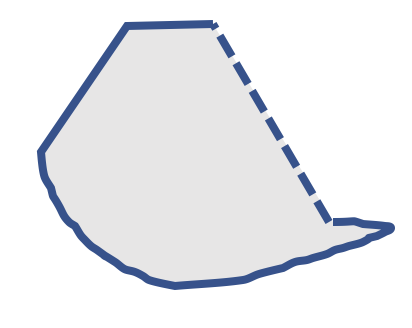
\includegraphics[width=\textwidth]{week2/p_1}
                \caption{Illustration of $A$}
                \label{fig:gull}
        \end{subfigure}%
        \begin{subfigure}[b]{0.3\textwidth}
                \centering
                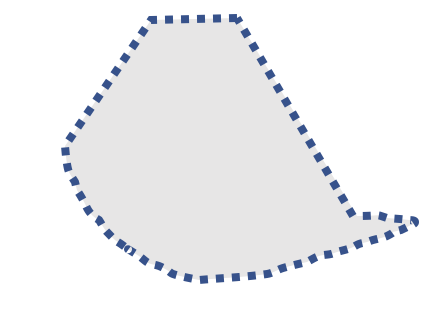
\includegraphics[width=\textwidth]{week2/p_2}
                \caption{Illustration of $A^\circ$}
                \label{fig:gull2}
        \end{subfigure}%
        \begin{subfigure}[b]{0.3\textwidth}
                \centering
                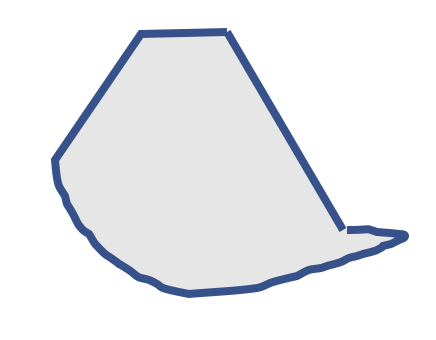
\includegraphics[width=\textwidth]{week2/p_3}
                \caption{Illustration of $\overline{A}$}
                \label{fig:tiger}
        \end{subfigure}
        \caption{Graph Illustrations}\label{fig:animals}
\end{figure}
\end{definition}
\begin{example}
\begin{enumerate}
\item

For $[a,b)\subseteq\mathbb{R}$, we have:
\[
\begin{array}{ll}
[a,b)^\circ=(a,b),
&
\overline{[a,b)}=[a,b]
\end{array}
\]

\item
For $X=\mathbb{R}$, $\mathbb{Q}^\circ=\emptyset$ and $\overline{\mathbb{Q}}=\mathbb{R}$.

\item
Consider the discrete topology $(X,\mathcal{T}_{\text{discrete}})$, we have
\[
\begin{array}{ll}
S^\circ=S,
&
\overline{S}=S
\end{array}
\]

\end{enumerate}
\end{example}

The insights behind the definition~(\ref{def:2:5}) is as follows

\begin{proposition}
\begin{enumerate}
\item
$A^\circ$ is the largest open subset of $X$ contained in $A$;

$\overline{A}$ is the smallest closed subset of $X$ containing $A$.
\item
If $A\subseteq B$, then $A^\circ\subseteq B$ and $\overline{A}\subseteq\overline{B}$
\item
$A$ is open in $X$ is equivalent to say $A^\circ = A$; $A$ is closed in $X$ is equivalent to say $\overline{A}=A$.
\end{enumerate}
\end{proposition}

\begin{example}
Let $(X,d)$ be a metric space. What's the closure of an open ball $B_r(x)$?

The direct intuition is to define the closed ball
\[
\bar B_r(x)=\{y\in X\mid d(x,y)\le r\}.
\]

Question: is $\bar B_r(x)=\overline{B_r(x)}$?
\begin{enumerate}
\item
Since $\bar B_r(x)$ is a closed subset of $X$, and 
$B_r(x)\subseteq \bar B_r(x)$, 
we imply that
\[
\overline{B_r(x)}\subseteq\bar B_r(x)
\]
\item
Howover, we may find an example such that $\overline{B_r(x)}$ is a proper subset of $\bar B_r(x)$:

Consider the discrete metric space $(X,d_{\text{discrete}})$ and for $\forall x\in X$,
\[
B_1(x)=\{x\}\implies
\overline{B_1(x)}=\{x\},\quad
\bar B_1(x)=X
\]

The equality $\bar B_r(x)=\overline{B_r(x)}$ holds when $(X,d)$ is a normed space.
\end{enumerate}
\end{example}

Here is another characterization of $\overline{A}$:

\begin{proposition}\label{pro:2:11}
\[
\overline{A}=\{x\in X\mid\forall \text{open }U\ni x, U\bigcap A\ne\emptyset\}
\]
\end{proposition}
\begin{proof}
Define
\[
S=\{x\in X\mid\forall \text{open }U\ni x, U\bigcap A\ne\emptyset\}
\]
It suffices to show that $\overline{A}=S$.
\begin{enumerate}
\item
First show that $S$ is closed:
\[
X\setminus S=\{x\in X\mid\exists U_x\ni x\text{ open s.t. }U_x\bigcap A=\emptyset\}
\]
Take $x\in X\setminus S$, we imply there exists open $U_x\ni x$ such that $U_x\bigcap A=\emptyset$. We claim $U_x\subseteq X\setminus S$:
\begin{itemize}
\item
For $\forall y\in U_x$, note that $U_x\ni y$ that is open, such that $U_x\bigcap A=\emptyset$. Therefore, $y\in X\setminus S$.
\end{itemize}

Therefore, we have $x\in U_x\subseteq X\setminus S$ for any $\forall x\in X\setminus S$.

Note that
\[
X\setminus S
=
\bigcup_{x\in X\setminus S}\{x\}\subseteq
\bigcup_{x\in X\setminus S}U_x\subseteq X\setminus S,
\]
which implies $X\setminus S=\bigcup_{x\in X\setminus S}U_x$ is open, i.e., $S$ is closed in $X$.
\item
By definition, it is clear that $A\subseteq S$:
\[
\forall a\in A,\forall\text{open }U\ni a,
U\bigcap A\supseteq\{a\}\ne\emptyset\implies a\in S.
\]
Therefore, $\overline{A}\subseteq\overline{S}=S$.
\item
Suppose on the contrary that 
there exists $y\in S\setminus\overline{A}$. 

Since $y\notin\overline{A}$, by definition, 
there exists $F\supseteq A$ closed such that 
$y\notin F$. 

Therefore, $y\in X\setminus F$ that is open, and 
\[
(X\setminus F)\bigcap A\subseteq(X\setminus A)\bigcap A=\emptyset\implies y\notin S,
\]
which is a contradiction. Therefore, $S=\overline{A}$.
\end{enumerate}
\end{proof}
\begin{definition}[accumulation point]
Let $A\subseteq X$ be a subset in a topological space. 
We call $x\in X$ are an 
\emph{accumulation point} (\emph{limit point}) of $A$ 
if
\[
\forall U\subseteq X\text{ open s.t. }
U\ni x, 
(U\setminus\{x\})\bigcap A\ne\emptyset.
\]

The set of accumulation points of $A$ is denoted as $A'$
\end{definition}
\begin{proposition}
$\overline{A}=A\bigcup A'$.
\end{proposition}

\begin{proof}
This proposition directly follows from Proposition~(\ref{pro:2:11}) and the definition of A'.
\end{proof}













\section{Wednesday for MAT3040}\index{Wednesday_lecture}
\subsection{Tensor Product for Linear Transformations}

\begin{proposition}
Suppose that $T:V\to V'$ and $S:W\to W'$ are linear transformations, then there exists an unique linear transformation 
\[
\begin{array}{ll}
T\otimes S:&V\otimes W\to V'\otimes W'\\
\text{satisfying}&(T\otimes S)(v\otimes w) = T(v)\otimes S(w)
\end{array}
\]
\end{proposition}

\begin{proof}
We construct the mapping
\[
\begin{array}{ll}
T\times S:&V\times W\to V'\otimes W'\\
\text{with}&(T\times S)(v,w) = T(v)\otimes S(w)
\end{array}
\]
This mapping is indeed bilinear: for instance, we can show that 
\[
(T\times S)(av_1+bv_2,w) = a(T\times S)(v_1,w)+b(T\times S)(v_2,w)
\]
Therefore, $T\times S\in\text{Obj}$. Since the tensor product satisfies the universal property, we imply there exists an unique linear transformation
\[
\begin{array}{ll}
T\otimes S&V\otimes W\to V'\otimes W'\\
\text{satisfying}&(T\otimes S)(v\otimes w)=T(v)\otimes S(w)
\end{array}
\]


\end{proof}
\paragraph{Notation Warning}
Does the notion $T\otimes S$ really form a tensor product, i.e., do we obtain the addictive rules for tensor product such as 
\[
(aT_1+bT_2)\otimes S = a(T_1\otimes S)+b(T_2\otimes S)?
\]


\begin{example}\label{exp:13:2}
Let $V=V'=\mathbb{F}^2$ and $W=W'=\mathbb{F}^3$.
Define the matrix-multiply mappings:
\[\left\{
\begin{array}{ll}
T:&V\to V\\
\text{with}&\bm v\mapsto\bm A\bm v\\
&\bm A=\begin{pmatrix}
a&b\\c&d
\end{pmatrix}
\end{array}\right.\qquad
\left\{
\begin{array}{ll}
S:&W\to W\\
\text{with}&\bm w\mapsto\bm B\bm w\\
&\bm B=\begin{pmatrix}
p&q&r\\
s&t&u\\
v&w&x
\end{pmatrix}
\end{array}
\right.
\]
How does $T\otimes S:V\otimes W\to V\otimes W$ look like?
\begin{itemize}
\item
Suppose $\{e_1,e_2\},\{f_1,f_2,f_3\}$ are usual basis of $V,W$, respectively.
Then the basis of $V\otimes W$ is given by:
\[
\mathcal{C}=\{e_1\otimes f_1,e_1\otimes f_2,e_1\otimes f_3,e_2\otimes f_1,e_2\otimes f_2,e_2\otimes f_3\}.
\]
\item
As a result, we can compute $(T\otimes S)(e_i\otimes f_j)$ for $i=1,2$ and $j=1,2,3$. For instance,
\begin{align*}
(T\otimes S)(e_1\otimes e_1)&=T(e_1)\otimes S(e_1)\\
&=(ae_1+ce_2)\otimes(pe_1+se_2+ve_3)\\
&=
(ap)e_1\otimes e_1+(as)e_1\otimes e_2+(av)e_1\otimes e_3+(cp)e_2\otimes e_1+(cs)e_2\otimes e_2+(cv)e_2\otimes e_3
\end{align*}
\item
Therefore, we obtain a matrix representation for the linear transformation $(T\otimes S)$:

\end{itemize}
We want a matrix representation for $(T\otimes S)$:
\[
(T\otimes S)_{\mathcal{C},\mathcal{C}}
=
\begin{pmatrix}
aB&bB\\
cB&dB
\end{pmatrix},
\]
which is a large matrix formed by taking all possible products between the elements of $\bm A$ and those of $\bm B$.
This operation is called the \emph{Kronecker Tensor Product}, see the command \textit{kron} in MATLAB for detail.


\end{example}
\begin{proposition}
More generally, given the linear operator $T:V\to V$ and $S:W\to W$, 
let $\mathcal{A}=\{v_1,\dots,v_n\},\mathcal{B}=\{w_1,\dots,w_m\}$ be a basis of $V,W$ respectively, with
\[
\begin{array}{ll}
(T)_{\mathcal{A},\mathcal{A}}=(a_{ij})
&
(S_{\mathcal{B},\mathcal{B}})=(b_{ij}):=B
\end{array}
\]
As a result, $(T\otimes S)_{\mathcal{C},\mathcal{C}}=A\otimes B$, where 
$\mathcal{C}=\{v_1\otimes w_1,\dots, v_n\otimes w_m\}$, and $A\otimes B$ denotes the Kronecker tensor product, defined as the matrix
\[
\begin{pmatrix}
a_{1,1}B&\cdots&a_{1,n}B\\
\vdots&\ddots&\vdots\\
a_{n,1}B&\cdots&a_{n,n}B
\end{pmatrix}.
\]
\end{proposition}
\begin{proof}
Following the similar procedure as in Example~(\ref{exp:13:2}) and applying the relation
\begin{align*}
(T\otimes S)(v_i\otimes w_j)&=T(v_i)\otimes S(w_j)\\
&=\left(
\sum_{k=1}^na_{ki}v_k
\right)
\otimes
\left(
\sum_{\ell=1}^mb_{\ell j}w_\ell
\right)\\
&=\sum_{k=1}^n\sum_{\ell=1}^m(a_{ki}b_{\ell j})v_k\otimes w_{\ell}
\end{align*}
\end{proof}

\begin{proposition}
The operation $T\otimes S$ satisfies all the properties of tensor product.
For example,
\begin{align*}
(aT_1+bT_2)\otimes S &= a(T_1\otimes S)+b(T_2\otimes S)\\
T\otimes(cS_1+dS_2) &= c(T\otimes S_1)+d(T\otimes S_2)
\end{align*}
Therefore, the usage of the notion ``$\otimes$'' is justified for the definition of $T\otimes S$.
\end{proposition}
\begin{proof}[Proof using matrix multiplication]
For instance, consider the operation $(T+T')\otimes S$, with $(T)_{\mathcal{A},\mathcal{A}}=(a_{ij})$, $(T')_{\mathcal{A},\mathcal{A}}=(c_{ij}), (S)_{\mathcal{B},\mathcal{B}}=B$.

We compute its matrix representation directly:
\begin{align*}
((T+T')\otimes S)_{\mathcal{C},\mathcal{C}}
&=
(T+T')_{\mathcal{A},\mathcal{A}}\otimes (S)_{\mathcal{B},\mathcal{B}}\\
&=
[(T)_{\mathcal{A},\mathcal{A}}+(T')_{\mathcal{A},\mathcal{A}}]\otimes (S)_{\mathcal{B},\mathcal{B}}\\
&=
(T)_{\mathcal{A},\mathcal{A}}\otimes (S)_{\mathcal{B},\mathcal{B}}
+
(T')_{\mathcal{A},\mathcal{A}}\otimes (S)_{\mathcal{B},\mathcal{B}}
\end{align*}
where the last equality is by the addictive rule for kronecker product for matrices.
Therefore,
\[
((T+T')\otimes S)_{\mathcal{C},\mathcal{C}}=
(T\otimes S)_{\mathcal{C},\mathcal{C}} + 
(T'\otimes S)_{\mathcal{C},\mathcal{C}}
\implies
(T+T')\otimes S
=
T\otimes S+T'\otimes S
\]
\end{proof}
\begin{proof}[Proof using basis of $T\otimes S$]
Another way of the proof is by computing 
\[
((T+T')\otimes S)(v_i\otimes w_j),
\] 
where $\{v_i\otimes w_j\mid 1\le i\le n,1\le j\le m\}$ forms a basis of $(T+T')\otimes S$:
\begin{align*}
((T+T')\otimes S)(v_i\otimes w_j)
&=(T+T')(v_i)\otimes S(w_j)\\
&=(T(v_i)+T'(v_i))\otimes S(w_j)\\
&=T(v_i)\otimes S(w_j)+T'(v_i)\otimes S(w_j)\\
&=(T\otimes S)(v_i\otimes w_j)+(T'\otimes S)(v_i\otimes w_j)
\end{align*}
Since $((T+T')\otimes S)(v_i\otimes w_j)$ coincides with $(T\otimes S + T'\otimes S)(v_i\otimes w_j)$ for all basis vectors $v_i\otimes w_j\in\mathcal{C}$, we imply
\[
(T+T')\otimes S = T\otimes S+T'\otimes S
\]
\end{proof}


\begin{proposition}
Let $A,C$ be linear operators from $V$ to $V$, and $B,D$ be linear operators from $W$ to $W$, then
\[
(A\otimes B)\circ(C\otimes D)=(AC)\otimes(BD)
\]
\end{proposition}

\begin{proposition}
Define linear operators $A:V\to V$ and $B:W\to W$ with $\dim(V),\dim(W)<\infty$.
Then
\[
\det(A\otimes B) = (\det(A))^{\dim(W)}(\det(B))^{\dim(V)}
\]
\end{proposition}

\begin{corollary}
There exists a linear transformation 
\[
\begin{array}{ll}
\Phi:&
\text{Hom}(V,V)\otimes\text{Hom}(W,W)\to
\text{Hom}(V\otimes W,V\otimes W)\\
\text{with}&A\otimes B\mapsto A\otimes B
\end{array}
\]
where the input of $\Phi$ is the tensor product of linear transformations, and the output is the linear transformation.
\end{corollary}
\begin{proof}
Construct the mapping
\[
\begin{array}{ll}
\Phi&:
\text{Hom}(V,V)\times\text{Hom}(W,W)\to
\text{Hom}(V\otimes W,V\otimes W)\\
\text{with}&\Phi(A,B)=A\otimes B
\end{array}
\]
The $\Phi$ is indeed bilinear: for instance, 
\begin{align*}
\Phi(pA+qC,B)&=(pA+qC)\otimes B\\
&=p(A\otimes B)+q(C\otimes B)\\
&=p\Phi(A,B)+q\Phi(C,B)
\end{align*}
This corollary follows from the universal property of tensor product.
\end{proof}
\begin{remark}
If assuming that $\dim(V),\dim(W)<\infty$, we imply
\begin{align*}
\dim(\text{Input space of $\Phi$})&=\dim(\text{Hom}(V,V))\dim(\text{Hom}(W,W))\\
&=
[\dim(V)\dim(V)]
\cdot
[\dim(W)\dim(W)]
=
[\dim(V)\dim(W)]^2\\
&=[\dim(V\otimes W)]^2\\
&=\dim(\text{Hom}(V\otimes W,V\otimes W))\\
&=\dim(\text{Output space of $\Phi$})
\end{align*}
Therefore, is $\Phi$ is an isomorphism?
If so, then every linear operator $\alpha:V\otimes W\to V\otimes W$ can be expressed as
\[
\alpha = A_1\otimes B_1+\cdots+A_k\otimes B_k
\]
where $A_i:V\to V$ and $B_j:W\to W$.
\end{remark}











\section{Wednesday for MAT3006}\index{Monday_lecture}
\paragraph{Reviewing}
\begin{itemize}
\item
Normed Space: a norm on a vector space
\item
Metric Space
\item
Open Ball
\end{itemize}
\subsection{Convergence of Sequences}
Since $\mathbb{R}^n$ and $\mathcal{C}[a,b]$ are both metric spaces, we can study the convergence in $\mathbb{R}^n$ and the functions defined on $[a,b]$ at the same time.

\begin{definition}[Convergence]
Let $(X,d)$ be a metric space. 
A sequence $\{x_n\}$ in $X$ is \emph{convergent} to $x$
if $\forall\varepsilon>0$, there exists $N\in\mathbb{N}$ such that
\[
d(x_n,x)<\varepsilon,\forall n\ge N.
\]
We can denote the convergence by
\[
\begin{array}{lllll}
x_n\to x,
&
\mbox{or}
&
\displaystyle
\lim_{n\to\infty}x_n=x,
&
\mbox{or}
&\displaystyle
\lim_{n\to\infty}d(x_n,x)=0
\end{array}
\]
\end{definition}
\begin{proposition}
If the limit of $\{x_n\}$ exists, then it is unique.
\end{proposition}
\begin{remark}
Note that the proposition above does not necessarily hold for topology spaces.
\end{remark}
\begin{proof}
Suppose $x_n\to x$ and $x_n\to y$, which implies
\[
0\le d(x,y)\le d(x,x_n)+d(x_n,y),\forall n
\]
Taking the limit $n\to\infty$ both sides, we imply $d(x,y)=0$, i.e., $x=y$.
\end{proof}
\begin{example}\label{Exp:1:16}
\begin{enumerate}
\item
Consider the metric space $(\mathbb{R}^k,d_\infty)$ and study the convergence
\begin{align*}
\lim_{n\to\infty}\bm x_n=\bm x&\Longleftrightarrow
\lim_{n\to\infty}\left(\max_{i=1\dots,k}|x_{n_i}-x_i|\right)=0\\
&\Longleftrightarrow
\lim_{n\to\infty}|x_{n_i}-x_i|=0,\forall i=1,\dots,k\\
&\Longleftrightarrow
\lim_{n\to\infty}x_{n_i}=x_i,
\end{align*}
i.e., the convergence defined in $d_\infty$ is the same as the convergence defined in $d_2$.
\item
Consider the convergence in the metric space $(\mathcal{C}[a,b],d_\infty)$:
\begin{align*}
\lim_{n\to\infty}f_n=f&\Longleftrightarrow
\lim_{n\to\infty}\left(\max_{[a,b]}|f_n(x)-f(x)|\right)=0\\
&\Longleftrightarrow
\forall\varepsilon>0,\forall x\in[a,b],\exists N_{\varepsilon}\mbox{ such that }|f_n(x)-f(x)|<\varepsilon,\forall n\ge N_{\varepsilon}
\end{align*}
which is equivalent to the uniform convergence of functions, i.e., the convergence defined in $d_2$.
\end{enumerate}
\end{example}
\begin{definition}[Equivalent metrics]
Let $d$ and $\rho$ be metrics on $X$. 
\begin{enumerate}
\item
We say $\rho$ is \emph{stronger} than $d$ (or $d$ is \emph{weaker} than $\rho$) if
\[
\exists K>0\mbox{ such that }d(x,y)\le K\rho(x,y),\forall x,y\in X
\]
\item
The metrics $d$ and $\rho$ are equivalent if there exists $K_1,K_2>0$ such that
\[
d(x,y)\le K_1\rho(x,y)\le K_2d(x,y)
\]
\end{enumerate}
\end{definition}
\begin{remark}
The strongerness of $\rho$ than $d$ is depiected in the graph below:
\begin{figure}[H]
\centering
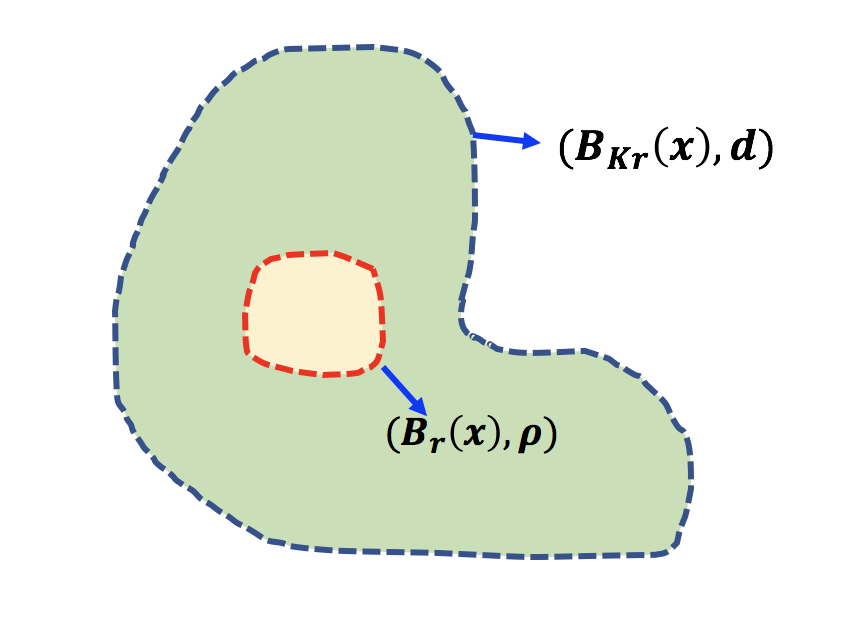
\includegraphics[width=8cm]{week1/f_3_1}
\caption{The open ball $(B_r(x),\rho)$ is contained by the open ball $(B_{Kr}(x),d)$}
\end{figure}
For each $x\in X$, consider the open ball $(B_r(x),\rho)$ and the open ball $(B_{Kr}(x),d)$:
\[
\begin{array}{ll}
B_r(x)=\{y\mid \rho(x,y)<r\},
&
B_{Kr}(x)=\{z\mid d(x,z)<Kr\}.
\end{array}
\]
For $y\in (B_r(x),\rho)$, we have $d(x,y)<K\rho(x,y)<Kr$, which implies $y\in (B_{Kr}(x),d)$, i.e, $(B_r(x),\rho)\subseteq (B_{Kr}(x),d)$ for any $x\in X$ and $r>0$.

\end{remark}
\begin{example}
\begin{enumerate}
\item
$d_1,d_2,d_\infty$ in $\mathbb{R}^n$ are equivalent
\begin{align*}
d_1(\bm x,\bm y)&\le d_\infty(\bm x,\bm y)\le nd_1(\bm x,\bm y)\\
d_2(\bm x,\bm y)&\le d_\infty(\bm x,\bm y)\le\sqrt{n}d_2(\bm x,\bm y)
\end{align*}
We use two relation depiected in the figure below to explain these two inequalities:
\begin{figure}[H]
\centering
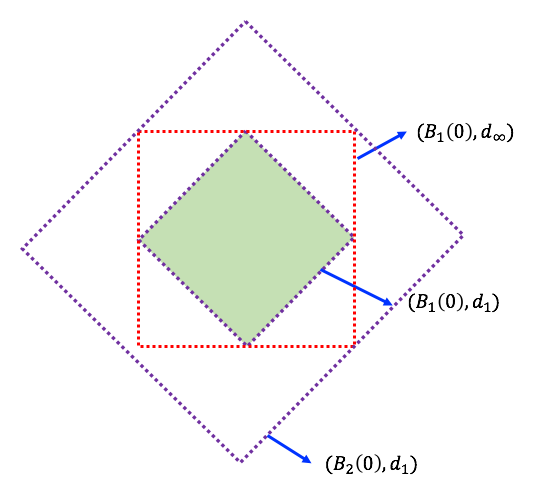
\includegraphics[width=8cm]{week1/f_3_2}
\caption{The diagram for the relation $(B_1(x),d_1)\subseteq(B_\infty(x),d_\infty)\subseteq (B_2(x),d_1)$ on $\mathbb{R}^2$}
\end{figure}
\begin{figure}[H]
\centering
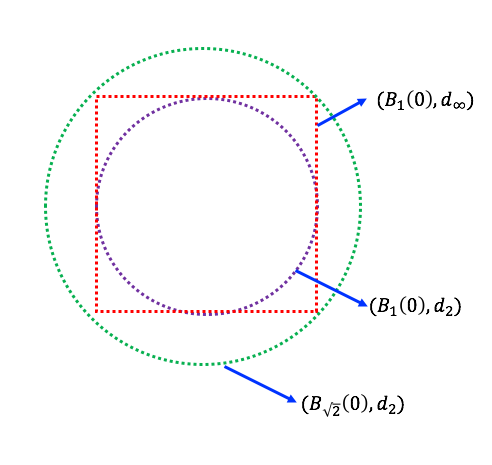
\includegraphics[width=8cm]{week1/f_3_3}
\caption{The diagram for the relation $(B_1(x),d_2)\subseteq(B_\infty(x),d_\infty)\subseteq (B_{\sqrt{2}}(x),d_2)$ on $\mathbb{R}^2$}
\end{figure}
It's easy to conclude the simple generalization for example~(\ref{Exp:1:16}):
\begin{proposition}
If $d$ and $\rho$ are equivalent, then 
\[
\lim_{n\to\infty}d(x_n,x)=0\Longleftrightarrow
\lim_{n\to\infty}\rho(x_n,x)=0
\]
\end{proposition}
Note that this does not necessarily hold for topology spaces.
\item
Consider $d_1,d_\infty$ in $\mathcal{C}[a,b]$:
\[
d_1(f,g):=\int_a^b|f-g|\diff x\le
\int_a^b\sup_{[a,b]}|f-g|\diff x=(b-a)d_\infty(f,g),
\]
i.e., $d_\infty$ is stronger than $d_1$. Question: Are they equivalent? \emph{No}.
\begin{proof}[Justification]
Consider $f_n(x)=n^2x^n(1-x)$ for $x\in[0,1]$. Check that
\[
\lim_{n\to\infty}d_1(f_n(x),0)=0,\quad
\mbox{but }d_\infty(f_n(x),0)\to\infty
\]
The peak of $f_n$ may go to infinite, while the integration converges to zero, i.e., there is no $K>0$ such that $d_{\infty}(f_n,0) < K d_1(f_n,0),\forall n\in\mathbb{N}$.
\end{proof}
We will discuss this topic at Lebsegue integration again.
\end{enumerate}
\end{example}
\subsection{Continuity}
\begin{definition}[Continuity]
Let $f:(X,d)\to(Y,d)$ be a function and $x_0\in X$. Then $f$ is continuous at $x_0$ if 
$\forall\varepsilon>0$, there exists $\delta>0$ such that
\[
d(x,x_0)<\delta\implies
\rho(f(x),f(x_0))<\varepsilon
\]
The function $f$ is continuous in $X$ if $f$ is continuous for all $x_0\in X$.
\end{definition}
\begin{proposition}\label{Pro:1:12}
The function $f$ is continuous at $x$ if and only if for all $\{x_n\}\to x$ under $d$, $f(x_n)\to f(x)$ under $\rho$.
\end{proposition}
\begin{proof}
\textit{Necessity:}
Given $\varepsilon>0$, by continuity, 
\begin{equation}\label{Eq:1:3}
d(x,x')<\delta\implies \rho(f(x'),f(x))<\varepsilon.
\end{equation}
Consider the sequence $\{x_n\}\to x$, then there exists $N$ such that $d(x_n,x)<\delta$ for $\forall n\ge N$. By applying (\ref{Eq:1:3}), $\rho(f(x_n),f(x))<\varepsilon$ for $\forall n\ge N$, i.e., $f(x_n)\to f(x)$.

\textit{Sufficiency}:
Assume that $f$ is not continuous at $x$, then there exists $\varepsilon_0$ such that for $\delta_n=\frac{1}{n}$, there exists $x_n$ such that
\[
d(x_n,x)<\delta_n,\mbox{ but }\rho(f(x_n),f(x))>\varepsilon_0.
\]
Then $\{x_n\}\to x$ by our construction, while $\{f(x_n)\}$ does not converge to $f(x)$, which is a contradiction.
\end{proof}
\begin{corollary}
If the function $f:(X,d)\to(Y,\rho)$ is continuous at $x$, the function $g:(Y,\rho)\to(Z,m)$ is continuous at $f(x)$,
then $g\circ f:(X,d)\to(Z,m)$ is continuous at $x$.
\end{corollary}
\begin{proof}
Note that
\[
\{x_n\}\to x
\xLongrightarrow{(a)}
\{f(x_n)\}\to f(x)
\xLongrightarrow{(b)}
\{g(f(x_n))\}\to g(f(x))
\xLongrightarrow{(c)}
g\circ f\mbox{ is continuous at $x$}.
\]
where $(a),(b),(c)$ are all by proposition~(\ref{Pro:1:12}).
\end{proof}
\subsection{Open and Closed Sets}
We have open/closed intervals in $\mathbb{R}$, and they are important in some theorems (e.g, continuous functions bring closed intervals to closed intervals).
\begin{definition}[Open]
Let $(X,d)$ be a metric space.  A set $U\subseteq X$ is open if for each $x\in U$, there exists $\rho_x>0$ such that $B_{\rho_x}(x)\subseteq U$. The empty set $\emptyset$ is defined to be open.
\end{definition}
\begin{example}
Let $(\mathbb{R},d_2\mbox{ or }d_\infty)$ be a metric space. The set $U=(a,b)$ is open.
\end{example}
\begin{proposition}
\begin{enumerate}
\item
Let $(X,d)$ be a metric space. Then all open balls $B_r(x)$ are open
\item
All open sets in $X$ can be written as a union of open balls.
\end{enumerate}
\end{proposition}
\begin{proof}
\begin{enumerate}
\item
Let $y\in B_r(x)$, i.e., $d(x,y):=q<r$. Consider the open ball $B_{(r-q)/2}(y)$. It suffices to show $B_{(r-q)/2}(y)\subseteq B_r(x)$. For any $z\in B_{(r-q)/2}(y)$,
\[
d(x,z)\le d(x,y)+d(y,z)<q+\frac{r-q}{2}=\frac{r+q}{2}<r.
\]
The proof is complete.
\item
Let $U\subseteq X$ be open, i.e., for $\forall x\in U$, there exists $\varepsilon_x>0$ such that $B_{\varepsilon_x}(x)\subseteq U$. Therefore
\[
\{x\}\subseteq B_{\varepsilon_x}(x)\subseteq U,\forall x\in U
\]
which implies
\[
U=\bigcup_{x\in U}\{x\}\subseteq \bigcup_{x\in U}B_{\varepsilon_x}(x)\subseteq U,
\]
i.e., $U=\bigcup_{x\in U}B_{\varepsilon_x}(x)$.
\end{enumerate}
\end{proof}

















\section{Wednesday for MAT4002}\index{Monday_lecture}
\subsection{Remarks on product space} 
\paragraph{Reviewing}
\begin{itemize}
\item
Product Topology: For topological space $(X,\mathcal{T}_X)$ and $(Y,\mathcal{Y})$, define the basis
\[
\mathcal{B}_{X\times Y}=\{U\times V\mid U\in\mathcal{T}_X,V\in\mathcal{T}_Y\}
\]
and the family of union of subsets in $\mathcal{B}_{X\times Y}$ forms a product topology.
\end{itemize}
\begin{proposition}
a ring torus is homeomorphic to the Cartesian product of two circles, say $S^1\times S^1\cong T$.
\end{proposition}
 \begin{proof}
 Define a mapping $f:[0,2\pi]\times [0,2\pi]\to T$ as
 \[
 f(\theta,\phi)=\begin{pmatrix}
(R+r\cos\theta)\cos\phi,
&
(R+r\cos\theta)\sin\phi,
&
r\sin\theta
\end{pmatrix}
 \]
Define $i:T\to\mathbb{R}^3$, we imply
 \[
 i\circ f:[0,2\pi]\times[0,2\pi]\to\mathbb{R}^3\ \text{is continuous}
 \]
 Therefore we imply $f:[0,2\pi]\times [0,2\pi]\to T$ is continuous. Together with the condition that 
\[
\left\{
\begin{aligned}
f(0,y)&=f(2\pi,y)\\
f(x,0)&=f(x,2\pi)
\end{aligned}
\right.
\]
we imply the function $f:S^1\times S^1\to T$ is continuous.
We can also show it is bijective. We can also show $f^{-1}$ is continuous.
 \end{proof}
 
\begin{proposition}
\begin{enumerate}
\item
Let $X\times Y$ be endowed with product topology. 
The projection mappings defined as
\begin{align*}
p_X:&X\times Y\to X,\ \text{with }p_X(x,y) = x\\
p_Y:&X\times Y\to Y,\ \text{with }p_Y(x,y)=y
\end{align*}
are continuous.
\item
(an equivalent definition for product topology)
The product topology is the \emph{coarest topology} on $X\times Y$ such that $p_X$ and $p_Y$ are both continuous.
\item
(an equivalent definition for product topology)
Let $Z$ be a topological space, then the product topology is the unique topology that the red and the blue line in the diagram commutes:
\begin{figure}[H]
\centering
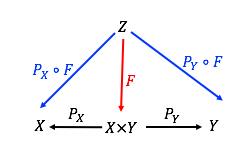
\includegraphics[width=6cm]{week3/p_3}
\caption{Diagram summarizing the statement~(*)}
\end{figure}
namely,
\begin{quotation}
\textit{
the mapping $F:Z\to X\times Y$ is continuous iff both $P_X\circ F:Z\to X$ and $P_Y\circ F:Z\to Y$ are continuous}. (*)
\end{quotation}
\end{enumerate}
\end{proposition}
\begin{proof}
\begin{enumerate}
\item
For any open $U$, we imply $p_X^{-1}(U)=U\times Y\in\mathcal{B}_{X\times Y}\subseteq\mathcal{T}_{X\times Y}$, i.e., $p_X^{-1}(U)$ is open. The same goes for $p_Y$.
\item
It suffices to show any topology $\mathcal{T}$ that meets the condition in (2) must contain $\mathcal{T}_{\text{product}}$. We imply that for $\forall U\in\mathcal{T}_X,V\in\mathcal{T}_Y$, 
\[
\left\{
\begin{aligned}
p_X^{-1}(U)&=U\times X\in\mathcal{T}\\
p_Y^{-1}(V)&=X\times V\in\mathcal{T}
\end{aligned}
\right.
\implies
(U\times Y)\cap(X\times V)=(U\cap X)\times (Y\cap V)=U\times V\in\mathcal{T},
\]
which implies $\mathcal{B}_{X\times Y}\subseteq\mathcal{T}$. Since $\mathcal{T}$ is closed for union operation on subsets, we imply $\mathcal{T}_{\text{product topology}}\subseteq\mathcal{T}$.
\item
\begin{enumerate}
\item
Firstly show that $\mathcal{T}_{\text{product}}$ satisfies (*).
\begin{itemize}
\item
For the forward direction, by (1) we imply both $p_X\circ F$ and $p_Y\circ F$ are continuous, since the composition of continuous functions are continuous as well.
\item
For the reverse direction, for $\forall U\times\mathcal{T}_X,V\in\mathcal{T}_Y$,
\[
F^{-1}(U\times V)=(p_X\circ F)^{-1}(X)\cap (p_Y\circ F)^{-1}(Y),
\]
which is open due to the continuity of $p_X\circ F$ and $p_Y\circ F$.
\end{itemize}
\item
Then we show the uniqueness of $\mathcal{T}_{\text{product}}$. Let $\mathcal{T}$ be another topology $X\times Y$ satisfying (*).
\begin{itemize}
\item
Take $Z=(X\times Y,\mathcal{T})$, and consider the identity mapping $F=\text{id}:Z\to Z$, which is continuous. Therefore $p_X\circ\text{id}$ and $p_Y\circ\text{id}$ are continuous, i.e., $p_X$ and $p_Y$ are continuous. By (2) we imply $\mathcal{T}_{\text{product}}\subseteq\mathcal{T}$.
\item
Take $Z=(X\times Y,\mathcal{T}_{\text{product}})$, and consider the identity mapping $F=\text{id}:Z\to Z$. Note that $p_X\circ F=p_X$ and $p_Y\circ F=p_Y$, which is continuous by (1). Therefore, the identity mapping $F:(X\times Y,\mathcal{T}_{\text{product}})\to(X\times Y,\mathcal{T})$ is continuous, which implies
\[
U=\text{id}^{-1}(U)\subseteq\mathcal{T}_{\text{product}}\ \text{for }\forall U\in\mathcal{T},
\]
i.e., $\mathcal{T}\subseteq\mathcal{T}_{\text{product}}.$
\end{itemize}
The proof is complete.
\end{enumerate}


\end{enumerate}
\end{proof}

\begin{definition}[Disjoint Union]
Let $X\times Y$ be two topological spaces, then the \emph{disjoint union} of $X$ and $Y$ is
\[
X\coprod Y:=(X\times\{0\})\cup(Y\times\{1\})
\]
\end{definition}
\begin{remark}
\begin{enumerate}
\item
We define that $U$ is open in $X\coprod Y$ if
\begin{enumerate}
\item
$U\cap(X\times\{0\})$ is open in $X\times\{0\}$; and
\item
$U\cap(Y\times\{1\})$ is open in $Y\times\{1\}$.
\end{enumerate}
We also need to show the well-definedness for this definition.
\item
$S$ is open in $X\coprod Y$ iff $S$ can be expressed as
\[
S=(U\times\{0\})\cup(V\times\{1\})
\]
where $U\subseteq X$ is open and $V\subseteq Y$ is open.
\end{enumerate}
\end{remark}


\subsection{Properties of Topological Spaces}
\subsubsection{Hausdorff Property}
\begin{definition}[First Separation Axiom]
A topological space $X$ satisfies the \emph{first separation axiom} if for any two distinct points $x\ne y\in X$, there exists open $U\ni x$ but not including $y$.
\end{definition}

\begin{proposition}
A topological space $X$ has first separation property if and only if for $\forall x\in X$, $\{x\}$ is closed in $X$.
\end{proposition}
\begin{proof}
\textit{Sufficiency.}
Suppose that $x\ne y$, then construct $U:=X\setminus\{y\}$, which is a open set that contains $x$ but not includes $y$.

\textit{Necessity.}
Take any $x\in X$, then for $\forall y\ne x$, there exists $y\in U_y$ that is open and $x\notin U_y$. Thus 
\[
\{y\}\subseteq U_y\subseteq X\setminus\{x\}
\]
which implies
\[
\bigcup_{y\in X\setminus\{x\}}\{y\}\subseteq
\bigcup_{y\in X\setminus\{x\}}U_y\subseteq
X\setminus\{x\},
\]
i.e., $X\setminus\{x\}=\bigcup_{y\in X\setminus\{x\}}U_y$ is open in $X$, i.e., $\{x\}$ is closed in $X.$
\end{proof}

\begin{definition}[Second separation Axiom]
A topological space satisfies the \emph{second separation axiom} (or $X$ is Hausdorff) if for all $x\ne y$ in $X$, there exists open sets $U,V$ such that
\[
\begin{array}{lll}
x\in U,
&
y\in V,
&
U\cap V=\emptyset
\end{array}
\]
\end{definition}

\begin{example}
All metrizable topological spaces are Hausdorff.

Suppose $d(x,y)=r>0$, then take $B_{r/2}(x)$ and $B_{r/2}(y)$
\end{example}

\begin{example}
Note that a topological space that is \emph{first separable} may not necessarily be \emph{second separable}:

Consider $\mathcal{T}_{\text{co-finite}}$, then $X$ is first separable but not Hausdorff:

Suppose on the contrary that for given $x\ne y$, there exists open sets $U,V$ such that $x\in U,y\in V$, and
\[
U\cap V=\emptyset\implies
X = X\setminus (U\cap V) = (X\setminus U)\cup(X\setminus V),
\]
implying that the union of two finite sets equals $X$, which is infinite, which is a contradiction.
\end{example}




















\chapter{Week4}
\section{Monday for MAT3040}\index{Monday_lecture}

\subsection{Quotient Spaces}

Now we aim to divide a big \emph{vector space} into many pieces of slices. 
\begin{itemize}
\item
For example, the Cartesian plane can be expressed as union of set of vertical lines as follows:
\[
\mathbb{R}^2 = \bigcup_{m\in\mathbb{R}}\left\{\begin{pmatrix}
m\\0
\end{pmatrix}+
\Span\{(0,1)\}\}
\right\}
\]
\item
Another example is that the set of integers can be expressed as union of three sets:
\[
\mathbb{Z}
=
Z_1\cup Z_2\cup Z_3,
\]
where $Z_i$ is the set of integers $z$ such that $z\text{ mod }3 = i$.
\end{itemize}

\begin{definition}[Coset]
Let $V$ be a vector space and $W\le V$. For any element $\bm v\in V$, the \emph{(right) coset} determined by $\bm v$ is the set
\[
\bm v+W:=\{\bm v+\bm w\mid\bm w\in W\}
\]
\end{definition}

For example, consider $V=\mathbb{R}^3$ and $W=\Span\{(1,2,0)\}$. Then the coset determined by $\bm v=(5,6,-3)$ can be written as
\[
\bm v+W=\left\{(5+t,6+2t,-3)\mid t\in\mathbb{R}\right\}
\]
It's interesting that the coset determined by $\bm v'=\{(4,4,-3)\}$ is exactly the same as the coset shown above:
\[
\bm v'+W=\left\{(4+t,4+2t,-3)\mid t\in\mathbb{R}\right\}=\bm v+W.
\]

Therefore, write the exact expression of $\bm v+W$ may sometimes become tedious and hard to check the equivalence. We say $\bm v$ is a \emph{representative} of a coset $\bm v+W$.

\begin{proposition}\label{pro:4:1}
Two cosets are the same iff the subtraction for the corresponding representatives is in $W$, i.e., 
\[
\bm v_1+W=\bm v_2+W
\Longleftrightarrow
\bm v_1-\bm v_2\in W
\]
\end{proposition}
\begin{proof}
\textit{Necessity.}
Suppose that $\bm v_1+W=\bm v_2+W$, then $\bm v_1+\bm w_1=\bm v_2+\bm w_2$ for some $\bm w_1,\bm w_2\in W$, which implies
\[
\bm v_1-\bm v_2=\bm w_2-\bm w_1\in W
\]
\textit{Sufficiency.}
Suppose that $\bm v_1-\bm v_2=\bm w\in W$. It suffices to show $\bm v_1+W\subseteq\bm v_2+W$.
For any $\bm v_1+\bm w'\in \bm v_1+W$, this element can be expressed as
\[
\bm v_1+\bm w'=(\bm v_2+\bm w)+\bm w'=\bm v_2+\underbrace{(\bm w+\bm w')}_{\text{belong to $W$}}\in \bm v_2+W.
\]
Therefore, $\bm v_1+W\subseteq \bm v_2+W$. Similarly we can show that $\bm v_2+W\subseteq \bm v_1+W$.
\end{proof}
\textit{Exercise: }Two cosets with representatives $\bm v_1,\bm v_2$ have no intersection iff $\bm v_1-\bm v_2\notin W$.

\begin{definition}[Quotient Space]
The \emph{quotient space} of $V$ by the subspace $W$, is the collection of all cosets $\bm v+W$, denoted by $V/ W$.
\end{definition}
To make the quotient space a vector space structure, we define the addition and scalar multiplication on $V/ W$ by:
\begin{align*}
(\bm v_1+W)+(\bm v_2+W)&:=(\bm v_1+\bm v_2)+W\\
\alpha\cdot (\bm v+W)&:=(\alpha\cdot\bm v) + W
\end{align*}

For example, consider $V=\mathbb{R}^2$ and $W=\Span\{(0,1)\}$. Then note that
\begin{align*}
\left(
\begin{pmatrix}
1\\0
\end{pmatrix}+W
\right)
+
\left(
\begin{pmatrix}
2\\0
\end{pmatrix}+W
\right)
&=
\left(
\begin{pmatrix}
3\\0
\end{pmatrix}+W
\right)\\
\pi\cdot\left(
\begin{pmatrix}
1\\0
\end{pmatrix}+W
\right)
&=
\left(
\begin{pmatrix}
\pi\\0
\end{pmatrix}+W
\right)
\end{align*}

\begin{proposition}
The addition and scalar multiplication is well-defined.
\end{proposition}
\begin{proof}
\begin{enumerate}
\item
Suppose that
\begin{equation}\label{Eq:4:1}
\left\{
\begin{aligned}
\bm v_1+W&=\bm v_1'+W\\
\bm v_2+W&=\bm v_2'+W
\end{aligned}
\right.,
\end{equation}
and we need to show that $(\bm v_1+\bm v_2)+W=(\bm v_1'+\bm v_2')+W$. 

From (\ref{Eq:4:1}) and proposition~(\ref{pro:4:1}), we imply
\[
\bm v_1-\bm v_1'\in W,\quad
\bm v_2-\bm v_2'\in W
\]
which implies
\[
(\bm v_1-\bm v_1')+(\bm v_2-\bm v_2')=(\bm v_1+\bm v_2) - (\bm v_1'+\bm v_2')\in W
\]

By proposition~(\ref{pro:4:1}) again we imply $(\bm v_1+\bm v_2)+W=(\bm v_1'+\bm v_2')+W$
\item
For scalar multiplication, similarly, we can show that $\bm v_1+W=\bm v_1'+W$ implies $\alpha\bm v_1+W=\alpha\bm v_1'+W$ for all $\alpha\in\mathbb{F}$.

\end{enumerate}

\end{proof}

\begin{proposition}
The canonical projection mapping
\[
\begin{aligned}
\pi_W:&V\to V/ W,\\
&\bm v\mapsto\bm v+W,
\end{aligned}
\]
is a \emph{surjective} \emph{linear transformation} with $\ker(\pi_W) = W$.
\end{proposition}
\begin{proof}
\begin{enumerate}
\item
First we show that $\ker(\pi_W)=W$:
\[
\pi_W(\bm v)=0\implies
\bm v+W=\bm0_{V/ W}\implies
\bm v+W=\bm0+W\implies \bm v=(\bm v-\bm0)\in W
\]
Here note that the zero element in the quotient space $V/ W$ is the coset with representative $\bm0$.
\item
For any $\bm v_0+W\in V/ W$, we can construct $\bm v_0\in V$ such that $\pi_W(\bm v_0)=\bm v_0+W$. Therefore the mapping $\pi_W$ is surjective.
\item
To show the mapping $\pi_W$ is a linear transformation, note that
\begin{align*}
\pi_W(\alpha\bm v_1+\beta\bm v_2)&=(\alpha\bm v_1+\beta\bm v_2)+W\\
&=(\alpha\bm v_1+W)+(\beta\bm v_2+W)\\
&=\alpha(\bm v_1+W)+\beta(\bm v_2+W)\\
&=\alpha\pi_W(\bm v_1)+\beta\pi_W(\bm v_2)
\end{align*}

\end{enumerate}


\end{proof}



\subsection{First Isomorphism Theorem}
The key of linear algebra is to solve the linear system $\bm A\bm x=\bm b$ with $\bm A\in\mathbb{R}^{m\times n}$. 
The general step for solving this linear system is as follows:
\begin{enumerate}
\item
Find the solution set for $\bm A\bm x=\bm0$, i.e., the set $\ker(\bm A)$
\item
Find a particular solution $\bm x_0$ such that $\bm A\bm x_0=\bm b$.
\end{enumerate}
Then the general solution set to this linear system is $\bm x_0+\ker(\bm A)$, which is a coset in the space $\mathbb{R}^n/ \ker(\bm A)$. Therefore, to solve the linear system $\bm{Ax}=\bm b$ suffices to study the quotient space $\mathbb{R}^n/ \ker(\bm A)$:

\begin{proposition}[Universal Property I]
Suppose that $T:V\to W$ is a linear transformation, and that $V'\le\ker(T)$. Then the mapping
\begin{align*}
\tilde{T}&:V/ V'\to W\\
&\bm v+V'\mapsto T(\bm v)
\end{align*}
is a well-defined linear transformation. As a result, the diagram below commutes:
\begin{figure}[H]
\centering
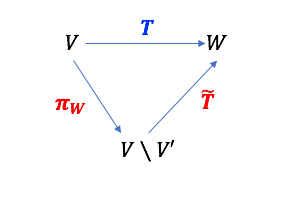
\includegraphics[width=0.5\textwidth]{week4/p_1}
\end{figure}
In other words, we have $T = \tilde{T}\circ \pi_W$.
\end{proposition}

\begin{proof}
First we show the well-definedness. Suppose that $\bm v_1+V'=\bm v_2+V'$ and suffices to show $\tilde T(\bm v_1+V')=\tilde T(\bm v_2+V')$, i.e., $T(\bm v_1)=T(\bm v_2)$. By proposition~(\ref{pro:4:1}), we imply
\[
\bm v_1-\bm v_2\in V'\le\ker(T)\implies
T(\bm v_1-\bm v_2)=\bm0\implies T(\bm v_1)-T(\bm v_2)=\bm0.
\]
Then we show $\tilde(T)$ is a linear transformation:
\begin{align*}
\tilde{T}(\alpha(\bm v_1+V')  + \beta(\bm v_2+V'))&=\tilde{T}((\alpha\bm v_1+\beta\bm v_2)+V')\\
&=T(\alpha\bm v_1+\beta\bm v_2)\\
&=\alpha T(\bm v_1)+\beta T(\bm v_2)\\
&=\alpha\tilde{T}(\bm v_1+V')+\beta\tilde{T}(\bm v_2+V')
\end{align*}
\end{proof}

Actually, if we let $V'=\ker(T)$, the mapping $\tilde{T}:V/ V'\to T(V)$ forms an isomorphism, In particular, if further $T$ is surjective, then $T(V)=W$, i.e., the mapping $\tilde{T}:V/ V'\to W$ forms an isomorphism.
\begin{theorem}[First Isomorphism Theorem]
Let $T:V\to W$ be a surjective linear transformation. Then the mapping 
\begin{align*}
\tilde{T}&:V/ \ker(T)\to W\\
&\bm v+\ker(T)\mapsto T(\bm v)
\end{align*}
is an isomorphism.
\end{theorem}
\begin{proof}
\textit{Injectivity.} Suppose that $\tilde{T}(\bm v_1+\ker(T)) = \tilde{T}(\bm v_2+\ker(T))$, then we imply
\[
T(\bm v_1)=T(\bm v_2)\implies T(\bm v_1-\bm v_2)=\bm0_W\implies\bm v_1-\bm v_2\in\ker(T),
\]
i.e., $\bm v_1+\ker(T)=\bm v_2+\ker(T)$.

\textit{Surjectivity.} For $\bm w\in W$, due to the surjectivity of $T$, we can find a $\bm v_0$ such that $T(\bm v_0)=\bm w$. Therefore, we can construct a set $\bm v_0+\ker(T)$ such that
\[
\tilde{T}(\bm v_0+\ker(T))=\bm w.
\]
\end{proof}




















\section{Monday for MAT3006}\index{Monday_lecture}
\subsection{Remarks on MCT}
\begin{example}
The MCT can help us to compute the integral
\begin{align*}
\lim_{n\to\infty}\int_{[0,n\pi]}\cos\left(\frac{x}{2n}\right)xe^{-x^2}\diff x
\end{align*}

Construct $f_n(x) = \cos\left(\frac{x}{2n}\right)xe^{-x^2}\mathcal{X}_{[0,n\pi]}$.
\begin{itemize}
\item
Since $\cos(x/2n)<\cos(x/2(n+1))$ for any $x\in[0,n\pi]$, we imply $f_n$ is monotone increasing with $n$
\item
$f_n(x)$ is integrable for all $n$.
\item
$f_n$ converges pointwise to $xe^{-x^2}\mathcal{X}_{[0,\infty)}$
\end{itemize}
Therefore, MCT I applies and
\[
\lim_{n\to\infty}\int_{[0,n\pi]}\cos\left(\frac{x}{2n}\right)xe^{-x^2}\diff x
=
\int\left(\lim_{n\to\infty}f_n\right)\diff m
\]
with
\[
\lim_{n\to\infty}f_n = xe^{-x^2}\mathcal{X}_{[0,\infty)}.
\]
Moreover, 
\begin{subequations}
\begin{align}
\int\left(\lim_{n\to\infty}f_n\right)\diff m &= 
\lim_{m\to\infty}\int_{[0,m]}xe^{-x^2}\diff x\label{Eq:12:1}\\
&=\int_0^\infty xe^{-x^2}\diff x\\
&=\frac{1}{2}
\end{align}
where (\ref{Eq:12:1}) is by applying MCT I with $g_m(x) = xe^{-x^2}\mathcal{X}_{[0,m]}$ and proposition~(\ref{pro:10:14}) to compute a Lebesgue integral by evaluating a proper Riemann integral.
\end{subequations}
\end{example}

Then we discuss the Lebesgue integral for series:

\begin{corollary}[Lebesgue Series Theorem]
Let $\{f_n\}$ be a series of measurable functions such that
\[
\sum_{n=1}^\infty\int|f_n|\diff m<\infty,
\]
then $\sum_{n=1}^kf_n$ converges to an integrable function $f = \sum_{n=1}^\infty f_n$ a.e., with
\[
\int f\diff m = \sum_{n=1}^\infty\int f_n\diff m
\]
\end{corollary}
\begin{proof}
\begin{itemize}
\item
For each $f_n$, consider 
\[
f_n = f_n^+ - f_n^-,\ \text{where $f_n^+,f_n^-$ are nonnegative}.
\]
By proposition~(\ref{pro:11:6}), 
\[
\int\sum_{n=1}^\infty f_n^+\diff m = \sum_{n=1}^\infty\int f_n^+\diff m\le \sum_{n=1}^\infty\int |f_n|\diff m<\infty.
\]
Therefore, $f^+:=\sum_{n=1}^\infty f_n^+=\lim_{k\to\infty}\sum_{n=1}^kf_n^+$ is integrable.
The same follows by replacing $f^{+}$ with $f^{-}$.
By corollary~(\ref{cor:9:6}), $f^+(x),f^-(x)<\infty,\forall x\in U$, where $U^c$ is null.
\item
Therefore, construct 
\[
f(x)=\left\{
\begin{aligned}
f^+(x)-f^-(x),&\quad x\in U\\
0,&\quad x\in U^c
\end{aligned}
\right.
\]
Moreover, for $x\in U$, 
\begin{align*}
f(x)&=\left(\lim_{k\to\infty}\sum_{n=1}^kf_n^+(x)\right)-
\left(\lim_{k\to\infty}\sum_{n=1}^kf_n^-(x)\right)\\
&=\lim_{k\to\infty}
\left(
\sum_{n=1}^kf_n^+(x)
-
\sum_{n=1}^kf_n^-(x)
\right)\\
&=\lim_{k\to\infty}\left[\sum_{n=1}^k(f_n^+(x)-f_n^-(x))\right]
\\&=
\sum_{n=1}^\infty f_n(x)
\end{align*}
where the first equality is because that both terms are finite.
\item
It follows that
\begin{subequations}
\begin{align}
\int f\diff m&=\int f^+\diff m - \int f^-\diff m\label{Eq:12:2:a}\\
&=
\int\sum_{n=1}^\infty f_n^+\diff m -\int\sum_{n=1}^\infty f_n^-\diff m\\
&=\left(\sum_{n=1}^\infty\int f_n^+\diff m\right)
-
\left(\sum_{n=1}^\infty\int f_n^-\diff m\right)\label{Eq:12:2:c}\\
&=\sum_{n=1}^\infty
\left(
\int f_n^+\diff m -\int f_n^-\diff m
\right)\label{Eq:12:2:d}\\
&=\sum_{n=1}^\infty\int f_n\diff m\label{Eq:12:2:e}
\end{align}
where (\ref{Eq:12:2:a}),(\ref{Eq:12:2:d}) is because that summation/subtraction between series holds when these series are finite; (\ref{Eq:12:2:c}) is by proposition~(\ref{pro:11:6}); (\ref{Eq:12:2:e}) is by definition of $f_n$.
\end{subequations}
\end{itemize}
\end{proof}

\begin{example}
Compute the integral
\[
\int_{(0,1]}e^{-x}x^{\alpha-1}\diff x,\ \alpha>0.
\]
\begin{itemize}
\item
Construct $f_n(x) = (-1)^n\frac{x^{\alpha+n-1}}{n!}\mathcal{X}_{(0,1]}, n\ge0$, and
\[
\sum_{n=0}^N f_n(x)\to e^{-x}x^{\alpha-1}, \ \text{pointwisely}, x\in(0,1]. 
\]
By applying MCT I,
\[
\int|f_n|\diff m=\frac{1}{(\alpha+n)n!}
\]
Therefore, 
\[
\sum_{n=0}^\infty\int|f_n|\diff m=
\sum_{n=0}^\infty\frac{1}{(\alpha+n)n!}<\infty
\]
\item
Applying the Lebesgue Series Theorem,
\[
\int_{(0,1]}e^{-x}x^{\alpha-1}\diff x = 
\int_{(0,1]}(\sum_{n=0}^\infty f_n)\diff m
=
\sum_{n=0}^\infty\int f_n\diff m=
\sum_{n=0}^\infty\frac{(-1)^n}{(\alpha+n)n!}
\]
\end{itemize}
\end{example}

\begin{remark}
It's essential to have $\sum\int|f|\diff m<\infty$ rather than $\sum\int f_n\diff m<\infty$ in the Lebesgue Series Theorem.
For example, let
\[
f_n=\frac{(-1)^{n+1}}{(n+1)}\mathcal{X}_{[n,n+1)}
\implies
\sum_{n=1}^\infty\int f_n\diff m =\log(2)<\infty
\]
However, $f:=\sum f_n$ is not integrable.
\end{remark}

\subsection{Dominated Convergence Theorem}
\begin{theorem}
Let $\{f_n\}$ be a sequence of measruable functions such that $|f_n|\le g$ a.e., and $g$ is integrable.
Suppose that $\lim_{n\to\infty}f_n(x)=f(x)$ a.e., then
\begin{enumerate}
\item
$f$ is integrable,
\item
\[
\int f\diff m =\lim_{n\to\infty}\int f_n\diff m
\]
\end{enumerate}
\end{theorem}
\begin{proof}
\begin{itemize}
\item
Observe that 
\[
|f_n|\le g\implies
\lim_{n\to\infty}|f_n|\le g\implies |f|\le g
\]
By comparison test, $g$ is integrable implies $|f|$ is integrable, and further $f$ is integrable.
\item
Consider the sequence of non-negative functions
$\{g-f_n\}_{n\in\mathbb{N}}$ and $\{g+f_n\}_{n\in\mathbb{N}}$.

By Fatou's Lemma, 
\begin{align*}
\lim_{n\to\infty}\inf\int(g-f_n)\diff m&\ge \int \lim_{n\to\infty}\inf(g-f_n)\diff m\\
&=\int(g-f)\diff m\\
&=\int g\diff m - \int f\diff m
\end{align*}
which follows that
\[
\int g\diff m - \lim_{n\to\infty}\sup\int f_n\diff m
\ge
\int g\diff m - \int f\diff m
\]
i.e.,
\[
\int f\diff m\ge  \lim_{n\to\infty}\sup\int f_n\diff m
\]
\item
Similarly, 
\[
\lim_{n\to\infty}\inf(g+f_n)\diff m\ge \int\lim_{n\to\infty}\inf(g+f_n)\diff m
=
\int g\diff m + \int f\diff m
\]
which implies
\[
 \lim_{n\to\infty}\inf\int f_n\diff m\ge\int f\diff m
\]
\end{itemize}
As a result,
\[
 \lim_{n\to\infty}\sup\int f_n\diff m
 \le
 \int f\diff m\le  \lim_{n\to\infty}\inf\int f_n\diff m,
\]
which implies
\[
\int f\diff m = \lim_n\int f_n\diff m
\]
\end{proof}

\begin{corollary}[Bounded Convergence Theorem]
Suppose that $E\in\mathcal{M}$ be such that $m(E)<\infty$.
If
\begin{itemize}
\item
$|f_n(x)|\le K<\infty$ for any $x\in E,n\in\mathbb{N}$
\item
$f_n\to f$ a.e. in $E$,
\end{itemize}
then $f$ is integrable in $E$ with
\[
\int_Ef\diff m = \lim_{n\to\infty}\int f_n\diff m
\]
\end{corollary}
\begin{proof}
Take $g=K\mathcal{X}_E$ in DCT.
\end{proof}


\begin{proposition}
Every Riemann integrable function $f$ on $[a,b]$ is Lebesgue integrable, without the condition that $f$ is continuous a.e.
\end{proposition}
\begin{proof}
Since $f$ is Riemann integrable, we imply $f$ is bounded.
We construct the Riemann lower abd upper functions with $2^n$ equal intervals, denoted as $\{\phi_n\}$ and $\{\psi_n\}$, which follows that
\begin{itemize}
\item
$\phi_n$ is monotone increasing;
$\psi_n$ is monotone decreasing;
\item
$\phi_n\le f\le \psi_n$, and
\[
\lim_{n\to\infty}\int_{[a,b]}\phi_n=\int_a^bf(x)\diff x = \lim_{n\to\infty}\int_{[a,b]}\psi_n.
\]
\end{itemize}
Construct $g=\sup_n\phi_n$ and $h=\inf_n\psi_n$.
Now we can apply the bounded convergence theorem:
\begin{itemize}
\item
$\phi_n$ is bounded on $[a,b]$
\item
$\phi_n\to g$ on $[a,b]$
\end{itemize}
which implies
$g$ is Lebesgue integrable on $[a,b]$, with 
\[
\int_{[a,b]}g\diff m = \lim_{n\to\infty}\int_{[a,b]}\phi_n\diff m=\int_a^bf(x)\diff x.
\]
Similarly, $h$ is Lebesgue integrable, with
\[
\int_{[a,b]}h\diff m = \lim_{n\to\infty}\int_{[a,b]}\psi_n\diff m=\int_a^bf(x)\diff x.
\]
Moreover, $g\le f\le h$, and
\[
\int_{[a,b]}(h-g)\diff m = \int_{[a,b]}h\diff m - \int_{[a,b]}g\diff m=\int_a^bf(x)\diff x-\int_a^bf(x)\diff x=0,
\]
which implies $h=g$ a.e., and further $f=g$ a.e., which implies
\[
\int_{[a,b]} f\diff m = \int_{[a,b]} g\diff m= \int_a^bf(x)\diff x.
\]
\end{proof}
\begin{remark}
However, an improper Riemann integral does not necessarily has the corresponding Lebesgue integral:
\[
f(x)=\sum_{n=1}^\infty (-1)^nn\cdot\mathcal{X}_{(1/(n+1),1/n]},\ x\in[0,1]
\]
In this case, $f$ is Riemann integrable but not Lebesgue integrable.
\end{remark}














\section{Monday for MAT4002}\index{Monday_lecture}

\paragraph{Reviewing}
\begin{enumerate}
\item
Topological Space $(X,\mathcal{J})$: a special class of topological space is that induced from metric space $(X,d)$:
\[
(X,\mathcal{T}),\quad\text{with }\mathcal{T}=\{\text{all open sets in $(X,d)$}\}
\]
\item
Closed Sets $(X\setminus U)$ with $U$ open.
\end{enumerate}

\begin{proposition}
Let $(X,\mathcal{T})$ be a topological space, 
\begin{enumerate}
\item
$\emptyset, X$ are closed in $X$
\item
$V_1,V_2$ closed in $X$ implies that $V_1\bigcup V_2$ closed in $X$
\item
$\{V_\alpha\mid\alpha\in\mathcal{A}\}$ closed in $X$ implies that $\bigcap_{\alpha\in\mathcal{A}}V_\alpha$ closed in $X$
\end{enumerate}
\end{proposition}
\begin{proof}
Applying the De Morgan's Law
\[
(X\setminus\bigcup_{i\in I}U_i)=\bigcap_{i\in I}(X\setminus U_i)
\]
\end{proof}

\subsection{Convergence in topological space}

\begin{definition}[Convergence]
A sequence $\{x_n\}$ of a topological space $(X,\mathcal{T})$ converges to $x\in X$ 
if $\forall U\ni x$ is open, there $\exists N$ such that $x_n\in U,\forall n\ge N$.
\end{definition}

\begin{example}
\begin{enumerate}
\item
The topology for the space $(X=\mathbb{R}^n,d_2)\to(X,\mathcal{T})$ (i.e., a topological space induced from meric space $(X=\mathbb{R}^n,d_2)$) is called a \emph{usual topology} on $\mathbb{R}^n$.

When I say $\mathbb{R}^n$ (or subset of $\mathbb{R}^n$) is a topological space, 
it is equipeed with usual topology.

Convergence of sequence in $(\mathbb{R}^n,\mathcal{T})$ is the usual convergence in analysis.

For $\mathbb{R}^n$ or metric space, the limit of sequence (if exists) is unique.

\item

Consider the topological space $(X,\mathcal{T}_{\text{indiscrete}})$. 
Take any sequence $\{x_n\}$ in $X$, it is convergent to any $x\in X$. 
Indeed, for $\forall U\ni x$ open, $U=X$. Therefore, 
\[
x_n\in U(=X),\forall n\ge1.
\]
\item

Consider the topological space $(X,\mathcal{T}_{\text{cofinite}})$, where $X$ is infinite. 
Consider $\{x_n\}$ is a sequence satisfying $m\ne n$ implies $x_m\ne x_n$. 
Then $\{x_n\}$ is convergent to any $x\in X$.

(Question: how to define openness for $\mathcal{T}_{\text{cofinite}}$ and $\mathcal{T}_{\text{indiscrete}})$?
\item

Consider the topological space $(X,\mathcal{T}_{\text{discrete}})$, 
the sequence $\{x_n\}\to x$ is equivalent to say $x_n=x$ for all sufficiently large $n$.
\end{enumerate}
\end{example}
\begin{remark}
The limit of sequences may not be unique. The reason is that ``$\mathcal{T}$ is not big enough''. We will give a criterion to make sure the limit is unique in the future. (Hausdorff)
\end{remark}
\begin{proposition}\label{pro:2:9}
If $F\subseteq(X,\mathcal{T})$ is closed, then for any convergent sequence $\{x_n\}$ in $F$, the limit(s) are also in $F$.
\end{proposition}

\begin{proof}
Let $\{x_n\}$ be a sequence in $F$ with limit $x\in X$. 
Suppose on the contrary that $x\notin F$ 
(i.e., $x\in X\setminus F$ that is open). 
There exists $N$ such that
\[
x_n\in X\setminus F,\forall n\ge N,
\]
i.e., $x_n\notin F$, which is a contradiction.
\end{proof}
\begin{remark}
The converse may not be true. If the $(X,\mathcal{T})$ is metrizable, the converse holds.

Counter-example: Consider the co-countable topological space $(X=\mathbb{R},\mathcal{T}_{\text{co-co}})$, where 
\[
\mathcal{T}_{\text{co-co}}=
\{U\mid X\setminus U\text{ is a countable set}\}
\bigcup\{\emptyset\},
\]
and $X$ is uncontable. 
Then note that $F=[0,1]\subsetneqq X$ is an un-countable set, and under co-countable topology, $F\supseteq \{x_n\}\to x$ implies $x_n=x\in F$ for all $n$.
It's clear that $X\setminus F\notin \mathcal{T}_{\text{co-co}}$, i.e., $F$ is not closed.
\end{remark}

\subsection{Interior, Closure, Boundary}
\begin{definition}\label{def:2:5}
Let $(X,\mathcal{T})$ be a topological space, and $A\subseteq X$ a subset.
\begin{enumerate}
\item
The \emph{interior} of $A$ is 
\[
A^\circ=\bigcup_{U\subseteq A,U\text{ is open}}U
\]
\item
The \emph{closure} of $A$ is
\[
\overline{A}=\bigcap_{A\subseteq V,V\text{ is closed}}V
\]
\end{enumerate}

If $\overline{A}=X$, we say that $A$ is dense in $X$.

The graph illustration of the definition above is as follows:
\begin{figure}[H]
        \begin{subfigure}[b]{0.3\textwidth}
                \centering
                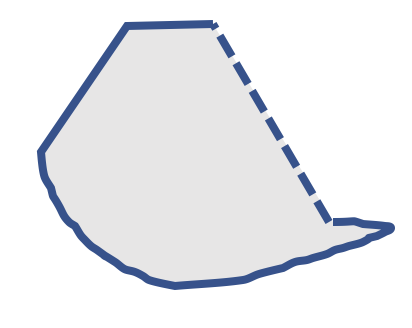
\includegraphics[width=\textwidth]{week2/p_1}
                \caption{Illustration of $A$}
                \label{fig:gull}
        \end{subfigure}%
        \begin{subfigure}[b]{0.3\textwidth}
                \centering
                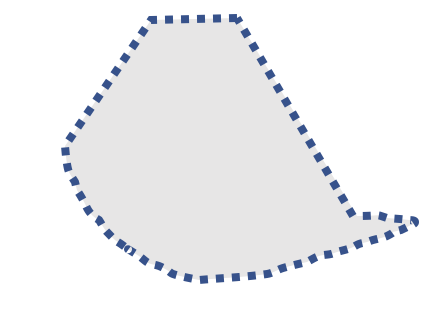
\includegraphics[width=\textwidth]{week2/p_2}
                \caption{Illustration of $A^\circ$}
                \label{fig:gull2}
        \end{subfigure}%
        \begin{subfigure}[b]{0.3\textwidth}
                \centering
                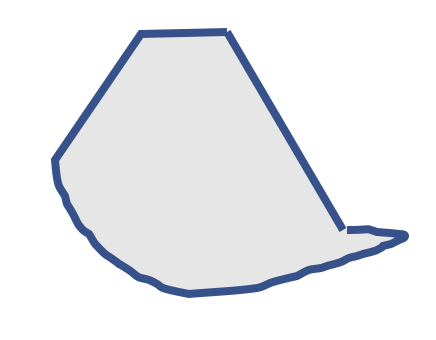
\includegraphics[width=\textwidth]{week2/p_3}
                \caption{Illustration of $\overline{A}$}
                \label{fig:tiger}
        \end{subfigure}
        \caption{Graph Illustrations}\label{fig:animals}
\end{figure}
\end{definition}
\begin{example}
\begin{enumerate}
\item

For $[a,b)\subseteq\mathbb{R}$, we have:
\[
\begin{array}{ll}
[a,b)^\circ=(a,b),
&
\overline{[a,b)}=[a,b]
\end{array}
\]

\item
For $X=\mathbb{R}$, $\mathbb{Q}^\circ=\emptyset$ and $\overline{\mathbb{Q}}=\mathbb{R}$.

\item
Consider the discrete topology $(X,\mathcal{T}_{\text{discrete}})$, we have
\[
\begin{array}{ll}
S^\circ=S,
&
\overline{S}=S
\end{array}
\]

\end{enumerate}
\end{example}

The insights behind the definition~(\ref{def:2:5}) is as follows

\begin{proposition}
\begin{enumerate}
\item
$A^\circ$ is the largest open subset of $X$ contained in $A$;

$\overline{A}$ is the smallest closed subset of $X$ containing $A$.
\item
If $A\subseteq B$, then $A^\circ\subseteq B$ and $\overline{A}\subseteq\overline{B}$
\item
$A$ is open in $X$ is equivalent to say $A^\circ = A$; $A$ is closed in $X$ is equivalent to say $\overline{A}=A$.
\end{enumerate}
\end{proposition}

\begin{example}
Let $(X,d)$ be a metric space. What's the closure of an open ball $B_r(x)$?

The direct intuition is to define the closed ball
\[
\bar B_r(x)=\{y\in X\mid d(x,y)\le r\}.
\]

Question: is $\bar B_r(x)=\overline{B_r(x)}$?
\begin{enumerate}
\item
Since $\bar B_r(x)$ is a closed subset of $X$, and 
$B_r(x)\subseteq \bar B_r(x)$, 
we imply that
\[
\overline{B_r(x)}\subseteq\bar B_r(x)
\]
\item
Howover, we may find an example such that $\overline{B_r(x)}$ is a proper subset of $\bar B_r(x)$:

Consider the discrete metric space $(X,d_{\text{discrete}})$ and for $\forall x\in X$,
\[
B_1(x)=\{x\}\implies
\overline{B_1(x)}=\{x\},\quad
\bar B_1(x)=X
\]

The equality $\bar B_r(x)=\overline{B_r(x)}$ holds when $(X,d)$ is a normed space.
\end{enumerate}
\end{example}

Here is another characterization of $\overline{A}$:

\begin{proposition}\label{pro:2:11}
\[
\overline{A}=\{x\in X\mid\forall \text{open }U\ni x, U\bigcap A\ne\emptyset\}
\]
\end{proposition}
\begin{proof}
Define
\[
S=\{x\in X\mid\forall \text{open }U\ni x, U\bigcap A\ne\emptyset\}
\]
It suffices to show that $\overline{A}=S$.
\begin{enumerate}
\item
First show that $S$ is closed:
\[
X\setminus S=\{x\in X\mid\exists U_x\ni x\text{ open s.t. }U_x\bigcap A=\emptyset\}
\]
Take $x\in X\setminus S$, we imply there exists open $U_x\ni x$ such that $U_x\bigcap A=\emptyset$. We claim $U_x\subseteq X\setminus S$:
\begin{itemize}
\item
For $\forall y\in U_x$, note that $U_x\ni y$ that is open, such that $U_x\bigcap A=\emptyset$. Therefore, $y\in X\setminus S$.
\end{itemize}

Therefore, we have $x\in U_x\subseteq X\setminus S$ for any $\forall x\in X\setminus S$.

Note that
\[
X\setminus S
=
\bigcup_{x\in X\setminus S}\{x\}\subseteq
\bigcup_{x\in X\setminus S}U_x\subseteq X\setminus S,
\]
which implies $X\setminus S=\bigcup_{x\in X\setminus S}U_x$ is open, i.e., $S$ is closed in $X$.
\item
By definition, it is clear that $A\subseteq S$:
\[
\forall a\in A,\forall\text{open }U\ni a,
U\bigcap A\supseteq\{a\}\ne\emptyset\implies a\in S.
\]
Therefore, $\overline{A}\subseteq\overline{S}=S$.
\item
Suppose on the contrary that 
there exists $y\in S\setminus\overline{A}$. 

Since $y\notin\overline{A}$, by definition, 
there exists $F\supseteq A$ closed such that 
$y\notin F$. 

Therefore, $y\in X\setminus F$ that is open, and 
\[
(X\setminus F)\bigcap A\subseteq(X\setminus A)\bigcap A=\emptyset\implies y\notin S,
\]
which is a contradiction. Therefore, $S=\overline{A}$.
\end{enumerate}
\end{proof}
\begin{definition}[accumulation point]
Let $A\subseteq X$ be a subset in a topological space. 
We call $x\in X$ are an 
\emph{accumulation point} (\emph{limit point}) of $A$ 
if
\[
\forall U\subseteq X\text{ open s.t. }
U\ni x, 
(U\setminus\{x\})\bigcap A\ne\emptyset.
\]

The set of accumulation points of $A$ is denoted as $A'$
\end{definition}
\begin{proposition}
$\overline{A}=A\bigcup A'$.
\end{proposition}

\begin{proof}
This proposition directly follows from Proposition~(\ref{pro:2:11}) and the definition of A'.
\end{proof}













\section{Wednesday for MAT3040}\index{Wednesday_lecture}
\subsection{Tensor Product for Linear Transformations}

\begin{proposition}
Suppose that $T:V\to V'$ and $S:W\to W'$ are linear transformations, then there exists an unique linear transformation 
\[
\begin{array}{ll}
T\otimes S:&V\otimes W\to V'\otimes W'\\
\text{satisfying}&(T\otimes S)(v\otimes w) = T(v)\otimes S(w)
\end{array}
\]
\end{proposition}

\begin{proof}
We construct the mapping
\[
\begin{array}{ll}
T\times S:&V\times W\to V'\otimes W'\\
\text{with}&(T\times S)(v,w) = T(v)\otimes S(w)
\end{array}
\]
This mapping is indeed bilinear: for instance, we can show that 
\[
(T\times S)(av_1+bv_2,w) = a(T\times S)(v_1,w)+b(T\times S)(v_2,w)
\]
Therefore, $T\times S\in\text{Obj}$. Since the tensor product satisfies the universal property, we imply there exists an unique linear transformation
\[
\begin{array}{ll}
T\otimes S&V\otimes W\to V'\otimes W'\\
\text{satisfying}&(T\otimes S)(v\otimes w)=T(v)\otimes S(w)
\end{array}
\]


\end{proof}
\paragraph{Notation Warning}
Does the notion $T\otimes S$ really form a tensor product, i.e., do we obtain the addictive rules for tensor product such as 
\[
(aT_1+bT_2)\otimes S = a(T_1\otimes S)+b(T_2\otimes S)?
\]


\begin{example}\label{exp:13:2}
Let $V=V'=\mathbb{F}^2$ and $W=W'=\mathbb{F}^3$.
Define the matrix-multiply mappings:
\[\left\{
\begin{array}{ll}
T:&V\to V\\
\text{with}&\bm v\mapsto\bm A\bm v\\
&\bm A=\begin{pmatrix}
a&b\\c&d
\end{pmatrix}
\end{array}\right.\qquad
\left\{
\begin{array}{ll}
S:&W\to W\\
\text{with}&\bm w\mapsto\bm B\bm w\\
&\bm B=\begin{pmatrix}
p&q&r\\
s&t&u\\
v&w&x
\end{pmatrix}
\end{array}
\right.
\]
How does $T\otimes S:V\otimes W\to V\otimes W$ look like?
\begin{itemize}
\item
Suppose $\{e_1,e_2\},\{f_1,f_2,f_3\}$ are usual basis of $V,W$, respectively.
Then the basis of $V\otimes W$ is given by:
\[
\mathcal{C}=\{e_1\otimes f_1,e_1\otimes f_2,e_1\otimes f_3,e_2\otimes f_1,e_2\otimes f_2,e_2\otimes f_3\}.
\]
\item
As a result, we can compute $(T\otimes S)(e_i\otimes f_j)$ for $i=1,2$ and $j=1,2,3$. For instance,
\begin{align*}
(T\otimes S)(e_1\otimes e_1)&=T(e_1)\otimes S(e_1)\\
&=(ae_1+ce_2)\otimes(pe_1+se_2+ve_3)\\
&=
(ap)e_1\otimes e_1+(as)e_1\otimes e_2+(av)e_1\otimes e_3+(cp)e_2\otimes e_1+(cs)e_2\otimes e_2+(cv)e_2\otimes e_3
\end{align*}
\item
Therefore, we obtain a matrix representation for the linear transformation $(T\otimes S)$:

\end{itemize}
We want a matrix representation for $(T\otimes S)$:
\[
(T\otimes S)_{\mathcal{C},\mathcal{C}}
=
\begin{pmatrix}
aB&bB\\
cB&dB
\end{pmatrix},
\]
which is a large matrix formed by taking all possible products between the elements of $\bm A$ and those of $\bm B$.
This operation is called the \emph{Kronecker Tensor Product}, see the command \textit{kron} in MATLAB for detail.


\end{example}
\begin{proposition}
More generally, given the linear operator $T:V\to V$ and $S:W\to W$, 
let $\mathcal{A}=\{v_1,\dots,v_n\},\mathcal{B}=\{w_1,\dots,w_m\}$ be a basis of $V,W$ respectively, with
\[
\begin{array}{ll}
(T)_{\mathcal{A},\mathcal{A}}=(a_{ij})
&
(S_{\mathcal{B},\mathcal{B}})=(b_{ij}):=B
\end{array}
\]
As a result, $(T\otimes S)_{\mathcal{C},\mathcal{C}}=A\otimes B$, where 
$\mathcal{C}=\{v_1\otimes w_1,\dots, v_n\otimes w_m\}$, and $A\otimes B$ denotes the Kronecker tensor product, defined as the matrix
\[
\begin{pmatrix}
a_{1,1}B&\cdots&a_{1,n}B\\
\vdots&\ddots&\vdots\\
a_{n,1}B&\cdots&a_{n,n}B
\end{pmatrix}.
\]
\end{proposition}
\begin{proof}
Following the similar procedure as in Example~(\ref{exp:13:2}) and applying the relation
\begin{align*}
(T\otimes S)(v_i\otimes w_j)&=T(v_i)\otimes S(w_j)\\
&=\left(
\sum_{k=1}^na_{ki}v_k
\right)
\otimes
\left(
\sum_{\ell=1}^mb_{\ell j}w_\ell
\right)\\
&=\sum_{k=1}^n\sum_{\ell=1}^m(a_{ki}b_{\ell j})v_k\otimes w_{\ell}
\end{align*}
\end{proof}

\begin{proposition}
The operation $T\otimes S$ satisfies all the properties of tensor product.
For example,
\begin{align*}
(aT_1+bT_2)\otimes S &= a(T_1\otimes S)+b(T_2\otimes S)\\
T\otimes(cS_1+dS_2) &= c(T\otimes S_1)+d(T\otimes S_2)
\end{align*}
Therefore, the usage of the notion ``$\otimes$'' is justified for the definition of $T\otimes S$.
\end{proposition}
\begin{proof}[Proof using matrix multiplication]
For instance, consider the operation $(T+T')\otimes S$, with $(T)_{\mathcal{A},\mathcal{A}}=(a_{ij})$, $(T')_{\mathcal{A},\mathcal{A}}=(c_{ij}), (S)_{\mathcal{B},\mathcal{B}}=B$.

We compute its matrix representation directly:
\begin{align*}
((T+T')\otimes S)_{\mathcal{C},\mathcal{C}}
&=
(T+T')_{\mathcal{A},\mathcal{A}}\otimes (S)_{\mathcal{B},\mathcal{B}}\\
&=
[(T)_{\mathcal{A},\mathcal{A}}+(T')_{\mathcal{A},\mathcal{A}}]\otimes (S)_{\mathcal{B},\mathcal{B}}\\
&=
(T)_{\mathcal{A},\mathcal{A}}\otimes (S)_{\mathcal{B},\mathcal{B}}
+
(T')_{\mathcal{A},\mathcal{A}}\otimes (S)_{\mathcal{B},\mathcal{B}}
\end{align*}
where the last equality is by the addictive rule for kronecker product for matrices.
Therefore,
\[
((T+T')\otimes S)_{\mathcal{C},\mathcal{C}}=
(T\otimes S)_{\mathcal{C},\mathcal{C}} + 
(T'\otimes S)_{\mathcal{C},\mathcal{C}}
\implies
(T+T')\otimes S
=
T\otimes S+T'\otimes S
\]
\end{proof}
\begin{proof}[Proof using basis of $T\otimes S$]
Another way of the proof is by computing 
\[
((T+T')\otimes S)(v_i\otimes w_j),
\] 
where $\{v_i\otimes w_j\mid 1\le i\le n,1\le j\le m\}$ forms a basis of $(T+T')\otimes S$:
\begin{align*}
((T+T')\otimes S)(v_i\otimes w_j)
&=(T+T')(v_i)\otimes S(w_j)\\
&=(T(v_i)+T'(v_i))\otimes S(w_j)\\
&=T(v_i)\otimes S(w_j)+T'(v_i)\otimes S(w_j)\\
&=(T\otimes S)(v_i\otimes w_j)+(T'\otimes S)(v_i\otimes w_j)
\end{align*}
Since $((T+T')\otimes S)(v_i\otimes w_j)$ coincides with $(T\otimes S + T'\otimes S)(v_i\otimes w_j)$ for all basis vectors $v_i\otimes w_j\in\mathcal{C}$, we imply
\[
(T+T')\otimes S = T\otimes S+T'\otimes S
\]
\end{proof}


\begin{proposition}
Let $A,C$ be linear operators from $V$ to $V$, and $B,D$ be linear operators from $W$ to $W$, then
\[
(A\otimes B)\circ(C\otimes D)=(AC)\otimes(BD)
\]
\end{proposition}

\begin{proposition}
Define linear operators $A:V\to V$ and $B:W\to W$ with $\dim(V),\dim(W)<\infty$.
Then
\[
\det(A\otimes B) = (\det(A))^{\dim(W)}(\det(B))^{\dim(V)}
\]
\end{proposition}

\begin{corollary}
There exists a linear transformation 
\[
\begin{array}{ll}
\Phi:&
\text{Hom}(V,V)\otimes\text{Hom}(W,W)\to
\text{Hom}(V\otimes W,V\otimes W)\\
\text{with}&A\otimes B\mapsto A\otimes B
\end{array}
\]
where the input of $\Phi$ is the tensor product of linear transformations, and the output is the linear transformation.
\end{corollary}
\begin{proof}
Construct the mapping
\[
\begin{array}{ll}
\Phi&:
\text{Hom}(V,V)\times\text{Hom}(W,W)\to
\text{Hom}(V\otimes W,V\otimes W)\\
\text{with}&\Phi(A,B)=A\otimes B
\end{array}
\]
The $\Phi$ is indeed bilinear: for instance, 
\begin{align*}
\Phi(pA+qC,B)&=(pA+qC)\otimes B\\
&=p(A\otimes B)+q(C\otimes B)\\
&=p\Phi(A,B)+q\Phi(C,B)
\end{align*}
This corollary follows from the universal property of tensor product.
\end{proof}
\begin{remark}
If assuming that $\dim(V),\dim(W)<\infty$, we imply
\begin{align*}
\dim(\text{Input space of $\Phi$})&=\dim(\text{Hom}(V,V))\dim(\text{Hom}(W,W))\\
&=
[\dim(V)\dim(V)]
\cdot
[\dim(W)\dim(W)]
=
[\dim(V)\dim(W)]^2\\
&=[\dim(V\otimes W)]^2\\
&=\dim(\text{Hom}(V\otimes W,V\otimes W))\\
&=\dim(\text{Output space of $\Phi$})
\end{align*}
Therefore, is $\Phi$ is an isomorphism?
If so, then every linear operator $\alpha:V\otimes W\to V\otimes W$ can be expressed as
\[
\alpha = A_1\otimes B_1+\cdots+A_k\otimes B_k
\]
where $A_i:V\to V$ and $B_j:W\to W$.
\end{remark}











\section{Wednesday for MAT3006}\index{Monday_lecture}
\paragraph{Reviewing}
\begin{itemize}
\item
Normed Space: a norm on a vector space
\item
Metric Space
\item
Open Ball
\end{itemize}
\subsection{Convergence of Sequences}
Since $\mathbb{R}^n$ and $\mathcal{C}[a,b]$ are both metric spaces, we can study the convergence in $\mathbb{R}^n$ and the functions defined on $[a,b]$ at the same time.

\begin{definition}[Convergence]
Let $(X,d)$ be a metric space. 
A sequence $\{x_n\}$ in $X$ is \emph{convergent} to $x$
if $\forall\varepsilon>0$, there exists $N\in\mathbb{N}$ such that
\[
d(x_n,x)<\varepsilon,\forall n\ge N.
\]
We can denote the convergence by
\[
\begin{array}{lllll}
x_n\to x,
&
\mbox{or}
&
\displaystyle
\lim_{n\to\infty}x_n=x,
&
\mbox{or}
&\displaystyle
\lim_{n\to\infty}d(x_n,x)=0
\end{array}
\]
\end{definition}
\begin{proposition}
If the limit of $\{x_n\}$ exists, then it is unique.
\end{proposition}
\begin{remark}
Note that the proposition above does not necessarily hold for topology spaces.
\end{remark}
\begin{proof}
Suppose $x_n\to x$ and $x_n\to y$, which implies
\[
0\le d(x,y)\le d(x,x_n)+d(x_n,y),\forall n
\]
Taking the limit $n\to\infty$ both sides, we imply $d(x,y)=0$, i.e., $x=y$.
\end{proof}
\begin{example}\label{Exp:1:16}
\begin{enumerate}
\item
Consider the metric space $(\mathbb{R}^k,d_\infty)$ and study the convergence
\begin{align*}
\lim_{n\to\infty}\bm x_n=\bm x&\Longleftrightarrow
\lim_{n\to\infty}\left(\max_{i=1\dots,k}|x_{n_i}-x_i|\right)=0\\
&\Longleftrightarrow
\lim_{n\to\infty}|x_{n_i}-x_i|=0,\forall i=1,\dots,k\\
&\Longleftrightarrow
\lim_{n\to\infty}x_{n_i}=x_i,
\end{align*}
i.e., the convergence defined in $d_\infty$ is the same as the convergence defined in $d_2$.
\item
Consider the convergence in the metric space $(\mathcal{C}[a,b],d_\infty)$:
\begin{align*}
\lim_{n\to\infty}f_n=f&\Longleftrightarrow
\lim_{n\to\infty}\left(\max_{[a,b]}|f_n(x)-f(x)|\right)=0\\
&\Longleftrightarrow
\forall\varepsilon>0,\forall x\in[a,b],\exists N_{\varepsilon}\mbox{ such that }|f_n(x)-f(x)|<\varepsilon,\forall n\ge N_{\varepsilon}
\end{align*}
which is equivalent to the uniform convergence of functions, i.e., the convergence defined in $d_2$.
\end{enumerate}
\end{example}
\begin{definition}[Equivalent metrics]
Let $d$ and $\rho$ be metrics on $X$. 
\begin{enumerate}
\item
We say $\rho$ is \emph{stronger} than $d$ (or $d$ is \emph{weaker} than $\rho$) if
\[
\exists K>0\mbox{ such that }d(x,y)\le K\rho(x,y),\forall x,y\in X
\]
\item
The metrics $d$ and $\rho$ are equivalent if there exists $K_1,K_2>0$ such that
\[
d(x,y)\le K_1\rho(x,y)\le K_2d(x,y)
\]
\end{enumerate}
\end{definition}
\begin{remark}
The strongerness of $\rho$ than $d$ is depiected in the graph below:
\begin{figure}[H]
\centering
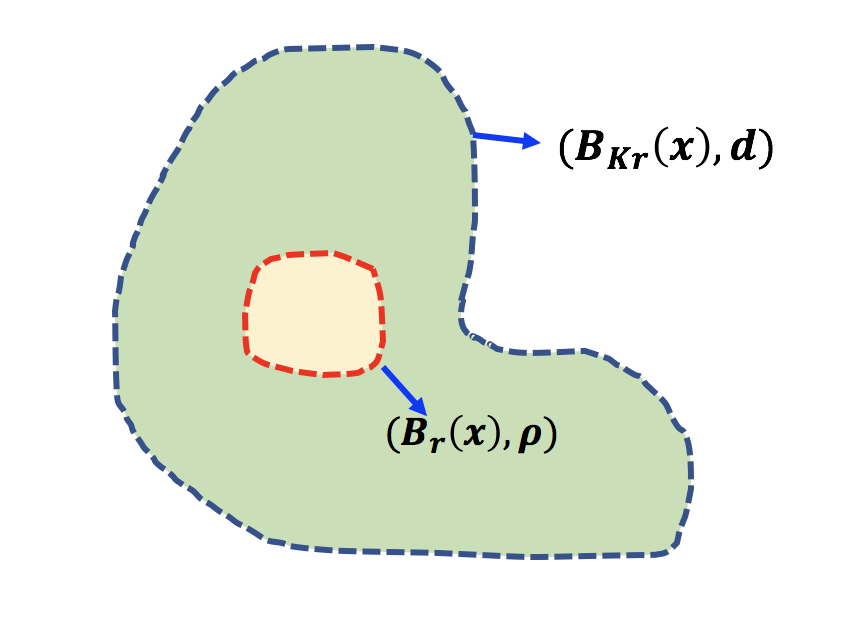
\includegraphics[width=8cm]{week1/f_3_1}
\caption{The open ball $(B_r(x),\rho)$ is contained by the open ball $(B_{Kr}(x),d)$}
\end{figure}
For each $x\in X$, consider the open ball $(B_r(x),\rho)$ and the open ball $(B_{Kr}(x),d)$:
\[
\begin{array}{ll}
B_r(x)=\{y\mid \rho(x,y)<r\},
&
B_{Kr}(x)=\{z\mid d(x,z)<Kr\}.
\end{array}
\]
For $y\in (B_r(x),\rho)$, we have $d(x,y)<K\rho(x,y)<Kr$, which implies $y\in (B_{Kr}(x),d)$, i.e, $(B_r(x),\rho)\subseteq (B_{Kr}(x),d)$ for any $x\in X$ and $r>0$.

\end{remark}
\begin{example}
\begin{enumerate}
\item
$d_1,d_2,d_\infty$ in $\mathbb{R}^n$ are equivalent
\begin{align*}
d_1(\bm x,\bm y)&\le d_\infty(\bm x,\bm y)\le nd_1(\bm x,\bm y)\\
d_2(\bm x,\bm y)&\le d_\infty(\bm x,\bm y)\le\sqrt{n}d_2(\bm x,\bm y)
\end{align*}
We use two relation depiected in the figure below to explain these two inequalities:
\begin{figure}[H]
\centering
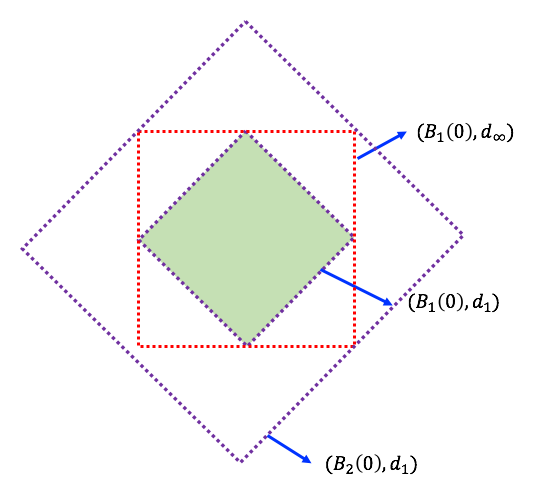
\includegraphics[width=8cm]{week1/f_3_2}
\caption{The diagram for the relation $(B_1(x),d_1)\subseteq(B_\infty(x),d_\infty)\subseteq (B_2(x),d_1)$ on $\mathbb{R}^2$}
\end{figure}
\begin{figure}[H]
\centering
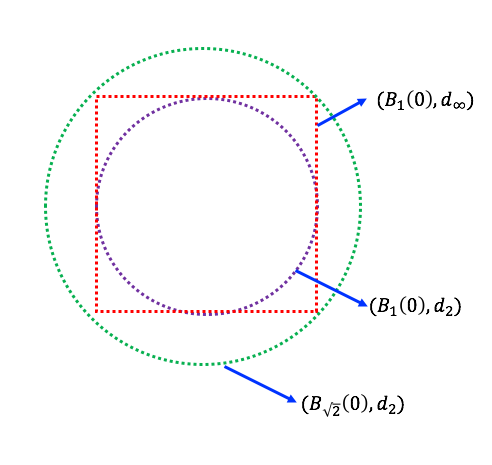
\includegraphics[width=8cm]{week1/f_3_3}
\caption{The diagram for the relation $(B_1(x),d_2)\subseteq(B_\infty(x),d_\infty)\subseteq (B_{\sqrt{2}}(x),d_2)$ on $\mathbb{R}^2$}
\end{figure}
It's easy to conclude the simple generalization for example~(\ref{Exp:1:16}):
\begin{proposition}
If $d$ and $\rho$ are equivalent, then 
\[
\lim_{n\to\infty}d(x_n,x)=0\Longleftrightarrow
\lim_{n\to\infty}\rho(x_n,x)=0
\]
\end{proposition}
Note that this does not necessarily hold for topology spaces.
\item
Consider $d_1,d_\infty$ in $\mathcal{C}[a,b]$:
\[
d_1(f,g):=\int_a^b|f-g|\diff x\le
\int_a^b\sup_{[a,b]}|f-g|\diff x=(b-a)d_\infty(f,g),
\]
i.e., $d_\infty$ is stronger than $d_1$. Question: Are they equivalent? \emph{No}.
\begin{proof}[Justification]
Consider $f_n(x)=n^2x^n(1-x)$ for $x\in[0,1]$. Check that
\[
\lim_{n\to\infty}d_1(f_n(x),0)=0,\quad
\mbox{but }d_\infty(f_n(x),0)\to\infty
\]
The peak of $f_n$ may go to infinite, while the integration converges to zero, i.e., there is no $K>0$ such that $d_{\infty}(f_n,0) < K d_1(f_n,0),\forall n\in\mathbb{N}$.
\end{proof}
We will discuss this topic at Lebsegue integration again.
\end{enumerate}
\end{example}
\subsection{Continuity}
\begin{definition}[Continuity]
Let $f:(X,d)\to(Y,d)$ be a function and $x_0\in X$. Then $f$ is continuous at $x_0$ if 
$\forall\varepsilon>0$, there exists $\delta>0$ such that
\[
d(x,x_0)<\delta\implies
\rho(f(x),f(x_0))<\varepsilon
\]
The function $f$ is continuous in $X$ if $f$ is continuous for all $x_0\in X$.
\end{definition}
\begin{proposition}\label{Pro:1:12}
The function $f$ is continuous at $x$ if and only if for all $\{x_n\}\to x$ under $d$, $f(x_n)\to f(x)$ under $\rho$.
\end{proposition}
\begin{proof}
\textit{Necessity:}
Given $\varepsilon>0$, by continuity, 
\begin{equation}\label{Eq:1:3}
d(x,x')<\delta\implies \rho(f(x'),f(x))<\varepsilon.
\end{equation}
Consider the sequence $\{x_n\}\to x$, then there exists $N$ such that $d(x_n,x)<\delta$ for $\forall n\ge N$. By applying (\ref{Eq:1:3}), $\rho(f(x_n),f(x))<\varepsilon$ for $\forall n\ge N$, i.e., $f(x_n)\to f(x)$.

\textit{Sufficiency}:
Assume that $f$ is not continuous at $x$, then there exists $\varepsilon_0$ such that for $\delta_n=\frac{1}{n}$, there exists $x_n$ such that
\[
d(x_n,x)<\delta_n,\mbox{ but }\rho(f(x_n),f(x))>\varepsilon_0.
\]
Then $\{x_n\}\to x$ by our construction, while $\{f(x_n)\}$ does not converge to $f(x)$, which is a contradiction.
\end{proof}
\begin{corollary}
If the function $f:(X,d)\to(Y,\rho)$ is continuous at $x$, the function $g:(Y,\rho)\to(Z,m)$ is continuous at $f(x)$,
then $g\circ f:(X,d)\to(Z,m)$ is continuous at $x$.
\end{corollary}
\begin{proof}
Note that
\[
\{x_n\}\to x
\xLongrightarrow{(a)}
\{f(x_n)\}\to f(x)
\xLongrightarrow{(b)}
\{g(f(x_n))\}\to g(f(x))
\xLongrightarrow{(c)}
g\circ f\mbox{ is continuous at $x$}.
\]
where $(a),(b),(c)$ are all by proposition~(\ref{Pro:1:12}).
\end{proof}
\subsection{Open and Closed Sets}
We have open/closed intervals in $\mathbb{R}$, and they are important in some theorems (e.g, continuous functions bring closed intervals to closed intervals).
\begin{definition}[Open]
Let $(X,d)$ be a metric space.  A set $U\subseteq X$ is open if for each $x\in U$, there exists $\rho_x>0$ such that $B_{\rho_x}(x)\subseteq U$. The empty set $\emptyset$ is defined to be open.
\end{definition}
\begin{example}
Let $(\mathbb{R},d_2\mbox{ or }d_\infty)$ be a metric space. The set $U=(a,b)$ is open.
\end{example}
\begin{proposition}
\begin{enumerate}
\item
Let $(X,d)$ be a metric space. Then all open balls $B_r(x)$ are open
\item
All open sets in $X$ can be written as a union of open balls.
\end{enumerate}
\end{proposition}
\begin{proof}
\begin{enumerate}
\item
Let $y\in B_r(x)$, i.e., $d(x,y):=q<r$. Consider the open ball $B_{(r-q)/2}(y)$. It suffices to show $B_{(r-q)/2}(y)\subseteq B_r(x)$. For any $z\in B_{(r-q)/2}(y)$,
\[
d(x,z)\le d(x,y)+d(y,z)<q+\frac{r-q}{2}=\frac{r+q}{2}<r.
\]
The proof is complete.
\item
Let $U\subseteq X$ be open, i.e., for $\forall x\in U$, there exists $\varepsilon_x>0$ such that $B_{\varepsilon_x}(x)\subseteq U$. Therefore
\[
\{x\}\subseteq B_{\varepsilon_x}(x)\subseteq U,\forall x\in U
\]
which implies
\[
U=\bigcup_{x\in U}\{x\}\subseteq \bigcup_{x\in U}B_{\varepsilon_x}(x)\subseteq U,
\]
i.e., $U=\bigcup_{x\in U}B_{\varepsilon_x}(x)$.
\end{enumerate}
\end{proof}

















\section{Wednesday for MAT4002}\index{Monday_lecture}
\subsection{Remarks on product space} 
\paragraph{Reviewing}
\begin{itemize}
\item
Product Topology: For topological space $(X,\mathcal{T}_X)$ and $(Y,\mathcal{Y})$, define the basis
\[
\mathcal{B}_{X\times Y}=\{U\times V\mid U\in\mathcal{T}_X,V\in\mathcal{T}_Y\}
\]
and the family of union of subsets in $\mathcal{B}_{X\times Y}$ forms a product topology.
\end{itemize}
\begin{proposition}
a ring torus is homeomorphic to the Cartesian product of two circles, say $S^1\times S^1\cong T$.
\end{proposition}
 \begin{proof}
 Define a mapping $f:[0,2\pi]\times [0,2\pi]\to T$ as
 \[
 f(\theta,\phi)=\begin{pmatrix}
(R+r\cos\theta)\cos\phi,
&
(R+r\cos\theta)\sin\phi,
&
r\sin\theta
\end{pmatrix}
 \]
Define $i:T\to\mathbb{R}^3$, we imply
 \[
 i\circ f:[0,2\pi]\times[0,2\pi]\to\mathbb{R}^3\ \text{is continuous}
 \]
 Therefore we imply $f:[0,2\pi]\times [0,2\pi]\to T$ is continuous. Together with the condition that 
\[
\left\{
\begin{aligned}
f(0,y)&=f(2\pi,y)\\
f(x,0)&=f(x,2\pi)
\end{aligned}
\right.
\]
we imply the function $f:S^1\times S^1\to T$ is continuous.
We can also show it is bijective. We can also show $f^{-1}$ is continuous.
 \end{proof}
 
\begin{proposition}
\begin{enumerate}
\item
Let $X\times Y$ be endowed with product topology. 
The projection mappings defined as
\begin{align*}
p_X:&X\times Y\to X,\ \text{with }p_X(x,y) = x\\
p_Y:&X\times Y\to Y,\ \text{with }p_Y(x,y)=y
\end{align*}
are continuous.
\item
(an equivalent definition for product topology)
The product topology is the \emph{coarest topology} on $X\times Y$ such that $p_X$ and $p_Y$ are both continuous.
\item
(an equivalent definition for product topology)
Let $Z$ be a topological space, then the product topology is the unique topology that the red and the blue line in the diagram commutes:
\begin{figure}[H]
\centering
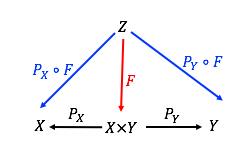
\includegraphics[width=6cm]{week3/p_3}
\caption{Diagram summarizing the statement~(*)}
\end{figure}
namely,
\begin{quotation}
\textit{
the mapping $F:Z\to X\times Y$ is continuous iff both $P_X\circ F:Z\to X$ and $P_Y\circ F:Z\to Y$ are continuous}. (*)
\end{quotation}
\end{enumerate}
\end{proposition}
\begin{proof}
\begin{enumerate}
\item
For any open $U$, we imply $p_X^{-1}(U)=U\times Y\in\mathcal{B}_{X\times Y}\subseteq\mathcal{T}_{X\times Y}$, i.e., $p_X^{-1}(U)$ is open. The same goes for $p_Y$.
\item
It suffices to show any topology $\mathcal{T}$ that meets the condition in (2) must contain $\mathcal{T}_{\text{product}}$. We imply that for $\forall U\in\mathcal{T}_X,V\in\mathcal{T}_Y$, 
\[
\left\{
\begin{aligned}
p_X^{-1}(U)&=U\times X\in\mathcal{T}\\
p_Y^{-1}(V)&=X\times V\in\mathcal{T}
\end{aligned}
\right.
\implies
(U\times Y)\cap(X\times V)=(U\cap X)\times (Y\cap V)=U\times V\in\mathcal{T},
\]
which implies $\mathcal{B}_{X\times Y}\subseteq\mathcal{T}$. Since $\mathcal{T}$ is closed for union operation on subsets, we imply $\mathcal{T}_{\text{product topology}}\subseteq\mathcal{T}$.
\item
\begin{enumerate}
\item
Firstly show that $\mathcal{T}_{\text{product}}$ satisfies (*).
\begin{itemize}
\item
For the forward direction, by (1) we imply both $p_X\circ F$ and $p_Y\circ F$ are continuous, since the composition of continuous functions are continuous as well.
\item
For the reverse direction, for $\forall U\times\mathcal{T}_X,V\in\mathcal{T}_Y$,
\[
F^{-1}(U\times V)=(p_X\circ F)^{-1}(X)\cap (p_Y\circ F)^{-1}(Y),
\]
which is open due to the continuity of $p_X\circ F$ and $p_Y\circ F$.
\end{itemize}
\item
Then we show the uniqueness of $\mathcal{T}_{\text{product}}$. Let $\mathcal{T}$ be another topology $X\times Y$ satisfying (*).
\begin{itemize}
\item
Take $Z=(X\times Y,\mathcal{T})$, and consider the identity mapping $F=\text{id}:Z\to Z$, which is continuous. Therefore $p_X\circ\text{id}$ and $p_Y\circ\text{id}$ are continuous, i.e., $p_X$ and $p_Y$ are continuous. By (2) we imply $\mathcal{T}_{\text{product}}\subseteq\mathcal{T}$.
\item
Take $Z=(X\times Y,\mathcal{T}_{\text{product}})$, and consider the identity mapping $F=\text{id}:Z\to Z$. Note that $p_X\circ F=p_X$ and $p_Y\circ F=p_Y$, which is continuous by (1). Therefore, the identity mapping $F:(X\times Y,\mathcal{T}_{\text{product}})\to(X\times Y,\mathcal{T})$ is continuous, which implies
\[
U=\text{id}^{-1}(U)\subseteq\mathcal{T}_{\text{product}}\ \text{for }\forall U\in\mathcal{T},
\]
i.e., $\mathcal{T}\subseteq\mathcal{T}_{\text{product}}.$
\end{itemize}
The proof is complete.
\end{enumerate}


\end{enumerate}
\end{proof}

\begin{definition}[Disjoint Union]
Let $X\times Y$ be two topological spaces, then the \emph{disjoint union} of $X$ and $Y$ is
\[
X\coprod Y:=(X\times\{0\})\cup(Y\times\{1\})
\]
\end{definition}
\begin{remark}
\begin{enumerate}
\item
We define that $U$ is open in $X\coprod Y$ if
\begin{enumerate}
\item
$U\cap(X\times\{0\})$ is open in $X\times\{0\}$; and
\item
$U\cap(Y\times\{1\})$ is open in $Y\times\{1\}$.
\end{enumerate}
We also need to show the well-definedness for this definition.
\item
$S$ is open in $X\coprod Y$ iff $S$ can be expressed as
\[
S=(U\times\{0\})\cup(V\times\{1\})
\]
where $U\subseteq X$ is open and $V\subseteq Y$ is open.
\end{enumerate}
\end{remark}


\subsection{Properties of Topological Spaces}
\subsubsection{Hausdorff Property}
\begin{definition}[First Separation Axiom]
A topological space $X$ satisfies the \emph{first separation axiom} if for any two distinct points $x\ne y\in X$, there exists open $U\ni x$ but not including $y$.
\end{definition}

\begin{proposition}
A topological space $X$ has first separation property if and only if for $\forall x\in X$, $\{x\}$ is closed in $X$.
\end{proposition}
\begin{proof}
\textit{Sufficiency.}
Suppose that $x\ne y$, then construct $U:=X\setminus\{y\}$, which is a open set that contains $x$ but not includes $y$.

\textit{Necessity.}
Take any $x\in X$, then for $\forall y\ne x$, there exists $y\in U_y$ that is open and $x\notin U_y$. Thus 
\[
\{y\}\subseteq U_y\subseteq X\setminus\{x\}
\]
which implies
\[
\bigcup_{y\in X\setminus\{x\}}\{y\}\subseteq
\bigcup_{y\in X\setminus\{x\}}U_y\subseteq
X\setminus\{x\},
\]
i.e., $X\setminus\{x\}=\bigcup_{y\in X\setminus\{x\}}U_y$ is open in $X$, i.e., $\{x\}$ is closed in $X.$
\end{proof}

\begin{definition}[Second separation Axiom]
A topological space satisfies the \emph{second separation axiom} (or $X$ is Hausdorff) if for all $x\ne y$ in $X$, there exists open sets $U,V$ such that
\[
\begin{array}{lll}
x\in U,
&
y\in V,
&
U\cap V=\emptyset
\end{array}
\]
\end{definition}

\begin{example}
All metrizable topological spaces are Hausdorff.

Suppose $d(x,y)=r>0$, then take $B_{r/2}(x)$ and $B_{r/2}(y)$
\end{example}

\begin{example}
Note that a topological space that is \emph{first separable} may not necessarily be \emph{second separable}:

Consider $\mathcal{T}_{\text{co-finite}}$, then $X$ is first separable but not Hausdorff:

Suppose on the contrary that for given $x\ne y$, there exists open sets $U,V$ such that $x\in U,y\in V$, and
\[
U\cap V=\emptyset\implies
X = X\setminus (U\cap V) = (X\setminus U)\cup(X\setminus V),
\]
implying that the union of two finite sets equals $X$, which is infinite, which is a contradiction.
\end{example}



















\chapter{Week4}
\section{Monday for MAT3040}\index{Monday_lecture}

\subsection{Quotient Spaces}

Now we aim to divide a big \emph{vector space} into many pieces of slices. 
\begin{itemize}
\item
For example, the Cartesian plane can be expressed as union of set of vertical lines as follows:
\[
\mathbb{R}^2 = \bigcup_{m\in\mathbb{R}}\left\{\begin{pmatrix}
m\\0
\end{pmatrix}+
\Span\{(0,1)\}\}
\right\}
\]
\item
Another example is that the set of integers can be expressed as union of three sets:
\[
\mathbb{Z}
=
Z_1\cup Z_2\cup Z_3,
\]
where $Z_i$ is the set of integers $z$ such that $z\text{ mod }3 = i$.
\end{itemize}

\begin{definition}[Coset]
Let $V$ be a vector space and $W\le V$. For any element $\bm v\in V$, the \emph{(right) coset} determined by $\bm v$ is the set
\[
\bm v+W:=\{\bm v+\bm w\mid\bm w\in W\}
\]
\end{definition}

For example, consider $V=\mathbb{R}^3$ and $W=\Span\{(1,2,0)\}$. Then the coset determined by $\bm v=(5,6,-3)$ can be written as
\[
\bm v+W=\left\{(5+t,6+2t,-3)\mid t\in\mathbb{R}\right\}
\]
It's interesting that the coset determined by $\bm v'=\{(4,4,-3)\}$ is exactly the same as the coset shown above:
\[
\bm v'+W=\left\{(4+t,4+2t,-3)\mid t\in\mathbb{R}\right\}=\bm v+W.
\]

Therefore, write the exact expression of $\bm v+W$ may sometimes become tedious and hard to check the equivalence. We say $\bm v$ is a \emph{representative} of a coset $\bm v+W$.

\begin{proposition}\label{pro:4:1}
Two cosets are the same iff the subtraction for the corresponding representatives is in $W$, i.e., 
\[
\bm v_1+W=\bm v_2+W
\Longleftrightarrow
\bm v_1-\bm v_2\in W
\]
\end{proposition}
\begin{proof}
\textit{Necessity.}
Suppose that $\bm v_1+W=\bm v_2+W$, then $\bm v_1+\bm w_1=\bm v_2+\bm w_2$ for some $\bm w_1,\bm w_2\in W$, which implies
\[
\bm v_1-\bm v_2=\bm w_2-\bm w_1\in W
\]
\textit{Sufficiency.}
Suppose that $\bm v_1-\bm v_2=\bm w\in W$. It suffices to show $\bm v_1+W\subseteq\bm v_2+W$.
For any $\bm v_1+\bm w'\in \bm v_1+W$, this element can be expressed as
\[
\bm v_1+\bm w'=(\bm v_2+\bm w)+\bm w'=\bm v_2+\underbrace{(\bm w+\bm w')}_{\text{belong to $W$}}\in \bm v_2+W.
\]
Therefore, $\bm v_1+W\subseteq \bm v_2+W$. Similarly we can show that $\bm v_2+W\subseteq \bm v_1+W$.
\end{proof}
\textit{Exercise: }Two cosets with representatives $\bm v_1,\bm v_2$ have no intersection iff $\bm v_1-\bm v_2\notin W$.

\begin{definition}[Quotient Space]
The \emph{quotient space} of $V$ by the subspace $W$, is the collection of all cosets $\bm v+W$, denoted by $V/ W$.
\end{definition}
To make the quotient space a vector space structure, we define the addition and scalar multiplication on $V/ W$ by:
\begin{align*}
(\bm v_1+W)+(\bm v_2+W)&:=(\bm v_1+\bm v_2)+W\\
\alpha\cdot (\bm v+W)&:=(\alpha\cdot\bm v) + W
\end{align*}

For example, consider $V=\mathbb{R}^2$ and $W=\Span\{(0,1)\}$. Then note that
\begin{align*}
\left(
\begin{pmatrix}
1\\0
\end{pmatrix}+W
\right)
+
\left(
\begin{pmatrix}
2\\0
\end{pmatrix}+W
\right)
&=
\left(
\begin{pmatrix}
3\\0
\end{pmatrix}+W
\right)\\
\pi\cdot\left(
\begin{pmatrix}
1\\0
\end{pmatrix}+W
\right)
&=
\left(
\begin{pmatrix}
\pi\\0
\end{pmatrix}+W
\right)
\end{align*}

\begin{proposition}
The addition and scalar multiplication is well-defined.
\end{proposition}
\begin{proof}
\begin{enumerate}
\item
Suppose that
\begin{equation}\label{Eq:4:1}
\left\{
\begin{aligned}
\bm v_1+W&=\bm v_1'+W\\
\bm v_2+W&=\bm v_2'+W
\end{aligned}
\right.,
\end{equation}
and we need to show that $(\bm v_1+\bm v_2)+W=(\bm v_1'+\bm v_2')+W$. 

From (\ref{Eq:4:1}) and proposition~(\ref{pro:4:1}), we imply
\[
\bm v_1-\bm v_1'\in W,\quad
\bm v_2-\bm v_2'\in W
\]
which implies
\[
(\bm v_1-\bm v_1')+(\bm v_2-\bm v_2')=(\bm v_1+\bm v_2) - (\bm v_1'+\bm v_2')\in W
\]

By proposition~(\ref{pro:4:1}) again we imply $(\bm v_1+\bm v_2)+W=(\bm v_1'+\bm v_2')+W$
\item
For scalar multiplication, similarly, we can show that $\bm v_1+W=\bm v_1'+W$ implies $\alpha\bm v_1+W=\alpha\bm v_1'+W$ for all $\alpha\in\mathbb{F}$.

\end{enumerate}

\end{proof}

\begin{proposition}
The canonical projection mapping
\[
\begin{aligned}
\pi_W:&V\to V/ W,\\
&\bm v\mapsto\bm v+W,
\end{aligned}
\]
is a \emph{surjective} \emph{linear transformation} with $\ker(\pi_W) = W$.
\end{proposition}
\begin{proof}
\begin{enumerate}
\item
First we show that $\ker(\pi_W)=W$:
\[
\pi_W(\bm v)=0\implies
\bm v+W=\bm0_{V/ W}\implies
\bm v+W=\bm0+W\implies \bm v=(\bm v-\bm0)\in W
\]
Here note that the zero element in the quotient space $V/ W$ is the coset with representative $\bm0$.
\item
For any $\bm v_0+W\in V/ W$, we can construct $\bm v_0\in V$ such that $\pi_W(\bm v_0)=\bm v_0+W$. Therefore the mapping $\pi_W$ is surjective.
\item
To show the mapping $\pi_W$ is a linear transformation, note that
\begin{align*}
\pi_W(\alpha\bm v_1+\beta\bm v_2)&=(\alpha\bm v_1+\beta\bm v_2)+W\\
&=(\alpha\bm v_1+W)+(\beta\bm v_2+W)\\
&=\alpha(\bm v_1+W)+\beta(\bm v_2+W)\\
&=\alpha\pi_W(\bm v_1)+\beta\pi_W(\bm v_2)
\end{align*}

\end{enumerate}


\end{proof}



\subsection{First Isomorphism Theorem}
The key of linear algebra is to solve the linear system $\bm A\bm x=\bm b$ with $\bm A\in\mathbb{R}^{m\times n}$. 
The general step for solving this linear system is as follows:
\begin{enumerate}
\item
Find the solution set for $\bm A\bm x=\bm0$, i.e., the set $\ker(\bm A)$
\item
Find a particular solution $\bm x_0$ such that $\bm A\bm x_0=\bm b$.
\end{enumerate}
Then the general solution set to this linear system is $\bm x_0+\ker(\bm A)$, which is a coset in the space $\mathbb{R}^n/ \ker(\bm A)$. Therefore, to solve the linear system $\bm{Ax}=\bm b$ suffices to study the quotient space $\mathbb{R}^n/ \ker(\bm A)$:

\begin{proposition}[Universal Property I]
Suppose that $T:V\to W$ is a linear transformation, and that $V'\le\ker(T)$. Then the mapping
\begin{align*}
\tilde{T}&:V/ V'\to W\\
&\bm v+V'\mapsto T(\bm v)
\end{align*}
is a well-defined linear transformation. As a result, the diagram below commutes:
\begin{figure}[H]
\centering
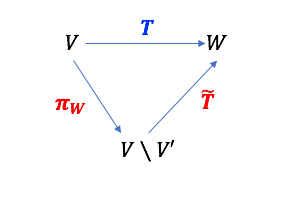
\includegraphics[width=0.5\textwidth]{week4/p_1}
\end{figure}
In other words, we have $T = \tilde{T}\circ \pi_W$.
\end{proposition}

\begin{proof}
First we show the well-definedness. Suppose that $\bm v_1+V'=\bm v_2+V'$ and suffices to show $\tilde T(\bm v_1+V')=\tilde T(\bm v_2+V')$, i.e., $T(\bm v_1)=T(\bm v_2)$. By proposition~(\ref{pro:4:1}), we imply
\[
\bm v_1-\bm v_2\in V'\le\ker(T)\implies
T(\bm v_1-\bm v_2)=\bm0\implies T(\bm v_1)-T(\bm v_2)=\bm0.
\]
Then we show $\tilde(T)$ is a linear transformation:
\begin{align*}
\tilde{T}(\alpha(\bm v_1+V')  + \beta(\bm v_2+V'))&=\tilde{T}((\alpha\bm v_1+\beta\bm v_2)+V')\\
&=T(\alpha\bm v_1+\beta\bm v_2)\\
&=\alpha T(\bm v_1)+\beta T(\bm v_2)\\
&=\alpha\tilde{T}(\bm v_1+V')+\beta\tilde{T}(\bm v_2+V')
\end{align*}
\end{proof}

Actually, if we let $V'=\ker(T)$, the mapping $\tilde{T}:V/ V'\to T(V)$ forms an isomorphism, In particular, if further $T$ is surjective, then $T(V)=W$, i.e., the mapping $\tilde{T}:V/ V'\to W$ forms an isomorphism.
\begin{theorem}[First Isomorphism Theorem]
Let $T:V\to W$ be a surjective linear transformation. Then the mapping 
\begin{align*}
\tilde{T}&:V/ \ker(T)\to W\\
&\bm v+\ker(T)\mapsto T(\bm v)
\end{align*}
is an isomorphism.
\end{theorem}
\begin{proof}
\textit{Injectivity.} Suppose that $\tilde{T}(\bm v_1+\ker(T)) = \tilde{T}(\bm v_2+\ker(T))$, then we imply
\[
T(\bm v_1)=T(\bm v_2)\implies T(\bm v_1-\bm v_2)=\bm0_W\implies\bm v_1-\bm v_2\in\ker(T),
\]
i.e., $\bm v_1+\ker(T)=\bm v_2+\ker(T)$.

\textit{Surjectivity.} For $\bm w\in W$, due to the surjectivity of $T$, we can find a $\bm v_0$ such that $T(\bm v_0)=\bm w$. Therefore, we can construct a set $\bm v_0+\ker(T)$ such that
\[
\tilde{T}(\bm v_0+\ker(T))=\bm w.
\]
\end{proof}




















\section{Monday for MAT3006}\index{Monday_lecture}
\subsection{Remarks on MCT}
\begin{example}
The MCT can help us to compute the integral
\begin{align*}
\lim_{n\to\infty}\int_{[0,n\pi]}\cos\left(\frac{x}{2n}\right)xe^{-x^2}\diff x
\end{align*}

Construct $f_n(x) = \cos\left(\frac{x}{2n}\right)xe^{-x^2}\mathcal{X}_{[0,n\pi]}$.
\begin{itemize}
\item
Since $\cos(x/2n)<\cos(x/2(n+1))$ for any $x\in[0,n\pi]$, we imply $f_n$ is monotone increasing with $n$
\item
$f_n(x)$ is integrable for all $n$.
\item
$f_n$ converges pointwise to $xe^{-x^2}\mathcal{X}_{[0,\infty)}$
\end{itemize}
Therefore, MCT I applies and
\[
\lim_{n\to\infty}\int_{[0,n\pi]}\cos\left(\frac{x}{2n}\right)xe^{-x^2}\diff x
=
\int\left(\lim_{n\to\infty}f_n\right)\diff m
\]
with
\[
\lim_{n\to\infty}f_n = xe^{-x^2}\mathcal{X}_{[0,\infty)}.
\]
Moreover, 
\begin{subequations}
\begin{align}
\int\left(\lim_{n\to\infty}f_n\right)\diff m &= 
\lim_{m\to\infty}\int_{[0,m]}xe^{-x^2}\diff x\label{Eq:12:1}\\
&=\int_0^\infty xe^{-x^2}\diff x\\
&=\frac{1}{2}
\end{align}
where (\ref{Eq:12:1}) is by applying MCT I with $g_m(x) = xe^{-x^2}\mathcal{X}_{[0,m]}$ and proposition~(\ref{pro:10:14}) to compute a Lebesgue integral by evaluating a proper Riemann integral.
\end{subequations}
\end{example}

Then we discuss the Lebesgue integral for series:

\begin{corollary}[Lebesgue Series Theorem]
Let $\{f_n\}$ be a series of measurable functions such that
\[
\sum_{n=1}^\infty\int|f_n|\diff m<\infty,
\]
then $\sum_{n=1}^kf_n$ converges to an integrable function $f = \sum_{n=1}^\infty f_n$ a.e., with
\[
\int f\diff m = \sum_{n=1}^\infty\int f_n\diff m
\]
\end{corollary}
\begin{proof}
\begin{itemize}
\item
For each $f_n$, consider 
\[
f_n = f_n^+ - f_n^-,\ \text{where $f_n^+,f_n^-$ are nonnegative}.
\]
By proposition~(\ref{pro:11:6}), 
\[
\int\sum_{n=1}^\infty f_n^+\diff m = \sum_{n=1}^\infty\int f_n^+\diff m\le \sum_{n=1}^\infty\int |f_n|\diff m<\infty.
\]
Therefore, $f^+:=\sum_{n=1}^\infty f_n^+=\lim_{k\to\infty}\sum_{n=1}^kf_n^+$ is integrable.
The same follows by replacing $f^{+}$ with $f^{-}$.
By corollary~(\ref{cor:9:6}), $f^+(x),f^-(x)<\infty,\forall x\in U$, where $U^c$ is null.
\item
Therefore, construct 
\[
f(x)=\left\{
\begin{aligned}
f^+(x)-f^-(x),&\quad x\in U\\
0,&\quad x\in U^c
\end{aligned}
\right.
\]
Moreover, for $x\in U$, 
\begin{align*}
f(x)&=\left(\lim_{k\to\infty}\sum_{n=1}^kf_n^+(x)\right)-
\left(\lim_{k\to\infty}\sum_{n=1}^kf_n^-(x)\right)\\
&=\lim_{k\to\infty}
\left(
\sum_{n=1}^kf_n^+(x)
-
\sum_{n=1}^kf_n^-(x)
\right)\\
&=\lim_{k\to\infty}\left[\sum_{n=1}^k(f_n^+(x)-f_n^-(x))\right]
\\&=
\sum_{n=1}^\infty f_n(x)
\end{align*}
where the first equality is because that both terms are finite.
\item
It follows that
\begin{subequations}
\begin{align}
\int f\diff m&=\int f^+\diff m - \int f^-\diff m\label{Eq:12:2:a}\\
&=
\int\sum_{n=1}^\infty f_n^+\diff m -\int\sum_{n=1}^\infty f_n^-\diff m\\
&=\left(\sum_{n=1}^\infty\int f_n^+\diff m\right)
-
\left(\sum_{n=1}^\infty\int f_n^-\diff m\right)\label{Eq:12:2:c}\\
&=\sum_{n=1}^\infty
\left(
\int f_n^+\diff m -\int f_n^-\diff m
\right)\label{Eq:12:2:d}\\
&=\sum_{n=1}^\infty\int f_n\diff m\label{Eq:12:2:e}
\end{align}
where (\ref{Eq:12:2:a}),(\ref{Eq:12:2:d}) is because that summation/subtraction between series holds when these series are finite; (\ref{Eq:12:2:c}) is by proposition~(\ref{pro:11:6}); (\ref{Eq:12:2:e}) is by definition of $f_n$.
\end{subequations}
\end{itemize}
\end{proof}

\begin{example}
Compute the integral
\[
\int_{(0,1]}e^{-x}x^{\alpha-1}\diff x,\ \alpha>0.
\]
\begin{itemize}
\item
Construct $f_n(x) = (-1)^n\frac{x^{\alpha+n-1}}{n!}\mathcal{X}_{(0,1]}, n\ge0$, and
\[
\sum_{n=0}^N f_n(x)\to e^{-x}x^{\alpha-1}, \ \text{pointwisely}, x\in(0,1]. 
\]
By applying MCT I,
\[
\int|f_n|\diff m=\frac{1}{(\alpha+n)n!}
\]
Therefore, 
\[
\sum_{n=0}^\infty\int|f_n|\diff m=
\sum_{n=0}^\infty\frac{1}{(\alpha+n)n!}<\infty
\]
\item
Applying the Lebesgue Series Theorem,
\[
\int_{(0,1]}e^{-x}x^{\alpha-1}\diff x = 
\int_{(0,1]}(\sum_{n=0}^\infty f_n)\diff m
=
\sum_{n=0}^\infty\int f_n\diff m=
\sum_{n=0}^\infty\frac{(-1)^n}{(\alpha+n)n!}
\]
\end{itemize}
\end{example}

\begin{remark}
It's essential to have $\sum\int|f|\diff m<\infty$ rather than $\sum\int f_n\diff m<\infty$ in the Lebesgue Series Theorem.
For example, let
\[
f_n=\frac{(-1)^{n+1}}{(n+1)}\mathcal{X}_{[n,n+1)}
\implies
\sum_{n=1}^\infty\int f_n\diff m =\log(2)<\infty
\]
However, $f:=\sum f_n$ is not integrable.
\end{remark}

\subsection{Dominated Convergence Theorem}
\begin{theorem}
Let $\{f_n\}$ be a sequence of measruable functions such that $|f_n|\le g$ a.e., and $g$ is integrable.
Suppose that $\lim_{n\to\infty}f_n(x)=f(x)$ a.e., then
\begin{enumerate}
\item
$f$ is integrable,
\item
\[
\int f\diff m =\lim_{n\to\infty}\int f_n\diff m
\]
\end{enumerate}
\end{theorem}
\begin{proof}
\begin{itemize}
\item
Observe that 
\[
|f_n|\le g\implies
\lim_{n\to\infty}|f_n|\le g\implies |f|\le g
\]
By comparison test, $g$ is integrable implies $|f|$ is integrable, and further $f$ is integrable.
\item
Consider the sequence of non-negative functions
$\{g-f_n\}_{n\in\mathbb{N}}$ and $\{g+f_n\}_{n\in\mathbb{N}}$.

By Fatou's Lemma, 
\begin{align*}
\lim_{n\to\infty}\inf\int(g-f_n)\diff m&\ge \int \lim_{n\to\infty}\inf(g-f_n)\diff m\\
&=\int(g-f)\diff m\\
&=\int g\diff m - \int f\diff m
\end{align*}
which follows that
\[
\int g\diff m - \lim_{n\to\infty}\sup\int f_n\diff m
\ge
\int g\diff m - \int f\diff m
\]
i.e.,
\[
\int f\diff m\ge  \lim_{n\to\infty}\sup\int f_n\diff m
\]
\item
Similarly, 
\[
\lim_{n\to\infty}\inf(g+f_n)\diff m\ge \int\lim_{n\to\infty}\inf(g+f_n)\diff m
=
\int g\diff m + \int f\diff m
\]
which implies
\[
 \lim_{n\to\infty}\inf\int f_n\diff m\ge\int f\diff m
\]
\end{itemize}
As a result,
\[
 \lim_{n\to\infty}\sup\int f_n\diff m
 \le
 \int f\diff m\le  \lim_{n\to\infty}\inf\int f_n\diff m,
\]
which implies
\[
\int f\diff m = \lim_n\int f_n\diff m
\]
\end{proof}

\begin{corollary}[Bounded Convergence Theorem]
Suppose that $E\in\mathcal{M}$ be such that $m(E)<\infty$.
If
\begin{itemize}
\item
$|f_n(x)|\le K<\infty$ for any $x\in E,n\in\mathbb{N}$
\item
$f_n\to f$ a.e. in $E$,
\end{itemize}
then $f$ is integrable in $E$ with
\[
\int_Ef\diff m = \lim_{n\to\infty}\int f_n\diff m
\]
\end{corollary}
\begin{proof}
Take $g=K\mathcal{X}_E$ in DCT.
\end{proof}


\begin{proposition}
Every Riemann integrable function $f$ on $[a,b]$ is Lebesgue integrable, without the condition that $f$ is continuous a.e.
\end{proposition}
\begin{proof}
Since $f$ is Riemann integrable, we imply $f$ is bounded.
We construct the Riemann lower abd upper functions with $2^n$ equal intervals, denoted as $\{\phi_n\}$ and $\{\psi_n\}$, which follows that
\begin{itemize}
\item
$\phi_n$ is monotone increasing;
$\psi_n$ is monotone decreasing;
\item
$\phi_n\le f\le \psi_n$, and
\[
\lim_{n\to\infty}\int_{[a,b]}\phi_n=\int_a^bf(x)\diff x = \lim_{n\to\infty}\int_{[a,b]}\psi_n.
\]
\end{itemize}
Construct $g=\sup_n\phi_n$ and $h=\inf_n\psi_n$.
Now we can apply the bounded convergence theorem:
\begin{itemize}
\item
$\phi_n$ is bounded on $[a,b]$
\item
$\phi_n\to g$ on $[a,b]$
\end{itemize}
which implies
$g$ is Lebesgue integrable on $[a,b]$, with 
\[
\int_{[a,b]}g\diff m = \lim_{n\to\infty}\int_{[a,b]}\phi_n\diff m=\int_a^bf(x)\diff x.
\]
Similarly, $h$ is Lebesgue integrable, with
\[
\int_{[a,b]}h\diff m = \lim_{n\to\infty}\int_{[a,b]}\psi_n\diff m=\int_a^bf(x)\diff x.
\]
Moreover, $g\le f\le h$, and
\[
\int_{[a,b]}(h-g)\diff m = \int_{[a,b]}h\diff m - \int_{[a,b]}g\diff m=\int_a^bf(x)\diff x-\int_a^bf(x)\diff x=0,
\]
which implies $h=g$ a.e., and further $f=g$ a.e., which implies
\[
\int_{[a,b]} f\diff m = \int_{[a,b]} g\diff m= \int_a^bf(x)\diff x.
\]
\end{proof}
\begin{remark}
However, an improper Riemann integral does not necessarily has the corresponding Lebesgue integral:
\[
f(x)=\sum_{n=1}^\infty (-1)^nn\cdot\mathcal{X}_{(1/(n+1),1/n]},\ x\in[0,1]
\]
In this case, $f$ is Riemann integrable but not Lebesgue integrable.
\end{remark}














\section{Monday for MAT4002}\index{Monday_lecture}

\paragraph{Reviewing}
\begin{enumerate}
\item
Topological Space $(X,\mathcal{J})$: a special class of topological space is that induced from metric space $(X,d)$:
\[
(X,\mathcal{T}),\quad\text{with }\mathcal{T}=\{\text{all open sets in $(X,d)$}\}
\]
\item
Closed Sets $(X\setminus U)$ with $U$ open.
\end{enumerate}

\begin{proposition}
Let $(X,\mathcal{T})$ be a topological space, 
\begin{enumerate}
\item
$\emptyset, X$ are closed in $X$
\item
$V_1,V_2$ closed in $X$ implies that $V_1\bigcup V_2$ closed in $X$
\item
$\{V_\alpha\mid\alpha\in\mathcal{A}\}$ closed in $X$ implies that $\bigcap_{\alpha\in\mathcal{A}}V_\alpha$ closed in $X$
\end{enumerate}
\end{proposition}
\begin{proof}
Applying the De Morgan's Law
\[
(X\setminus\bigcup_{i\in I}U_i)=\bigcap_{i\in I}(X\setminus U_i)
\]
\end{proof}

\subsection{Convergence in topological space}

\begin{definition}[Convergence]
A sequence $\{x_n\}$ of a topological space $(X,\mathcal{T})$ converges to $x\in X$ 
if $\forall U\ni x$ is open, there $\exists N$ such that $x_n\in U,\forall n\ge N$.
\end{definition}

\begin{example}
\begin{enumerate}
\item
The topology for the space $(X=\mathbb{R}^n,d_2)\to(X,\mathcal{T})$ (i.e., a topological space induced from meric space $(X=\mathbb{R}^n,d_2)$) is called a \emph{usual topology} on $\mathbb{R}^n$.

When I say $\mathbb{R}^n$ (or subset of $\mathbb{R}^n$) is a topological space, 
it is equipeed with usual topology.

Convergence of sequence in $(\mathbb{R}^n,\mathcal{T})$ is the usual convergence in analysis.

For $\mathbb{R}^n$ or metric space, the limit of sequence (if exists) is unique.

\item

Consider the topological space $(X,\mathcal{T}_{\text{indiscrete}})$. 
Take any sequence $\{x_n\}$ in $X$, it is convergent to any $x\in X$. 
Indeed, for $\forall U\ni x$ open, $U=X$. Therefore, 
\[
x_n\in U(=X),\forall n\ge1.
\]
\item

Consider the topological space $(X,\mathcal{T}_{\text{cofinite}})$, where $X$ is infinite. 
Consider $\{x_n\}$ is a sequence satisfying $m\ne n$ implies $x_m\ne x_n$. 
Then $\{x_n\}$ is convergent to any $x\in X$.

(Question: how to define openness for $\mathcal{T}_{\text{cofinite}}$ and $\mathcal{T}_{\text{indiscrete}})$?
\item

Consider the topological space $(X,\mathcal{T}_{\text{discrete}})$, 
the sequence $\{x_n\}\to x$ is equivalent to say $x_n=x$ for all sufficiently large $n$.
\end{enumerate}
\end{example}
\begin{remark}
The limit of sequences may not be unique. The reason is that ``$\mathcal{T}$ is not big enough''. We will give a criterion to make sure the limit is unique in the future. (Hausdorff)
\end{remark}
\begin{proposition}\label{pro:2:9}
If $F\subseteq(X,\mathcal{T})$ is closed, then for any convergent sequence $\{x_n\}$ in $F$, the limit(s) are also in $F$.
\end{proposition}

\begin{proof}
Let $\{x_n\}$ be a sequence in $F$ with limit $x\in X$. 
Suppose on the contrary that $x\notin F$ 
(i.e., $x\in X\setminus F$ that is open). 
There exists $N$ such that
\[
x_n\in X\setminus F,\forall n\ge N,
\]
i.e., $x_n\notin F$, which is a contradiction.
\end{proof}
\begin{remark}
The converse may not be true. If the $(X,\mathcal{T})$ is metrizable, the converse holds.

Counter-example: Consider the co-countable topological space $(X=\mathbb{R},\mathcal{T}_{\text{co-co}})$, where 
\[
\mathcal{T}_{\text{co-co}}=
\{U\mid X\setminus U\text{ is a countable set}\}
\bigcup\{\emptyset\},
\]
and $X$ is uncontable. 
Then note that $F=[0,1]\subsetneqq X$ is an un-countable set, and under co-countable topology, $F\supseteq \{x_n\}\to x$ implies $x_n=x\in F$ for all $n$.
It's clear that $X\setminus F\notin \mathcal{T}_{\text{co-co}}$, i.e., $F$ is not closed.
\end{remark}

\subsection{Interior, Closure, Boundary}
\begin{definition}\label{def:2:5}
Let $(X,\mathcal{T})$ be a topological space, and $A\subseteq X$ a subset.
\begin{enumerate}
\item
The \emph{interior} of $A$ is 
\[
A^\circ=\bigcup_{U\subseteq A,U\text{ is open}}U
\]
\item
The \emph{closure} of $A$ is
\[
\overline{A}=\bigcap_{A\subseteq V,V\text{ is closed}}V
\]
\end{enumerate}

If $\overline{A}=X$, we say that $A$ is dense in $X$.

The graph illustration of the definition above is as follows:
\begin{figure}[H]
        \begin{subfigure}[b]{0.3\textwidth}
                \centering
                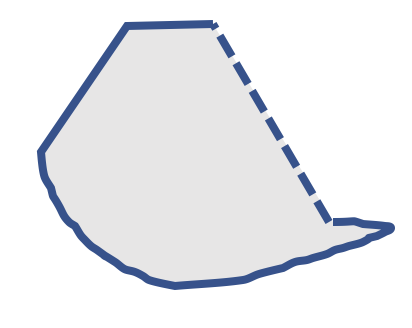
\includegraphics[width=\textwidth]{week2/p_1}
                \caption{Illustration of $A$}
                \label{fig:gull}
        \end{subfigure}%
        \begin{subfigure}[b]{0.3\textwidth}
                \centering
                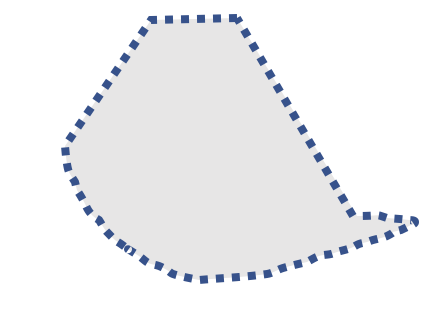
\includegraphics[width=\textwidth]{week2/p_2}
                \caption{Illustration of $A^\circ$}
                \label{fig:gull2}
        \end{subfigure}%
        \begin{subfigure}[b]{0.3\textwidth}
                \centering
                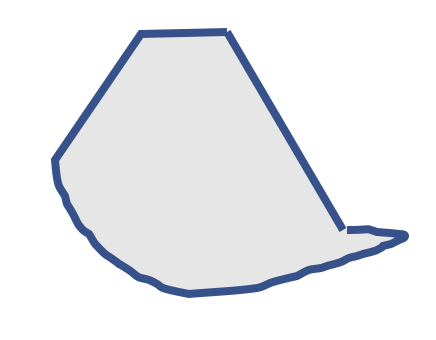
\includegraphics[width=\textwidth]{week2/p_3}
                \caption{Illustration of $\overline{A}$}
                \label{fig:tiger}
        \end{subfigure}
        \caption{Graph Illustrations}\label{fig:animals}
\end{figure}
\end{definition}
\begin{example}
\begin{enumerate}
\item

For $[a,b)\subseteq\mathbb{R}$, we have:
\[
\begin{array}{ll}
[a,b)^\circ=(a,b),
&
\overline{[a,b)}=[a,b]
\end{array}
\]

\item
For $X=\mathbb{R}$, $\mathbb{Q}^\circ=\emptyset$ and $\overline{\mathbb{Q}}=\mathbb{R}$.

\item
Consider the discrete topology $(X,\mathcal{T}_{\text{discrete}})$, we have
\[
\begin{array}{ll}
S^\circ=S,
&
\overline{S}=S
\end{array}
\]

\end{enumerate}
\end{example}

The insights behind the definition~(\ref{def:2:5}) is as follows

\begin{proposition}
\begin{enumerate}
\item
$A^\circ$ is the largest open subset of $X$ contained in $A$;

$\overline{A}$ is the smallest closed subset of $X$ containing $A$.
\item
If $A\subseteq B$, then $A^\circ\subseteq B$ and $\overline{A}\subseteq\overline{B}$
\item
$A$ is open in $X$ is equivalent to say $A^\circ = A$; $A$ is closed in $X$ is equivalent to say $\overline{A}=A$.
\end{enumerate}
\end{proposition}

\begin{example}
Let $(X,d)$ be a metric space. What's the closure of an open ball $B_r(x)$?

The direct intuition is to define the closed ball
\[
\bar B_r(x)=\{y\in X\mid d(x,y)\le r\}.
\]

Question: is $\bar B_r(x)=\overline{B_r(x)}$?
\begin{enumerate}
\item
Since $\bar B_r(x)$ is a closed subset of $X$, and 
$B_r(x)\subseteq \bar B_r(x)$, 
we imply that
\[
\overline{B_r(x)}\subseteq\bar B_r(x)
\]
\item
Howover, we may find an example such that $\overline{B_r(x)}$ is a proper subset of $\bar B_r(x)$:

Consider the discrete metric space $(X,d_{\text{discrete}})$ and for $\forall x\in X$,
\[
B_1(x)=\{x\}\implies
\overline{B_1(x)}=\{x\},\quad
\bar B_1(x)=X
\]

The equality $\bar B_r(x)=\overline{B_r(x)}$ holds when $(X,d)$ is a normed space.
\end{enumerate}
\end{example}

Here is another characterization of $\overline{A}$:

\begin{proposition}\label{pro:2:11}
\[
\overline{A}=\{x\in X\mid\forall \text{open }U\ni x, U\bigcap A\ne\emptyset\}
\]
\end{proposition}
\begin{proof}
Define
\[
S=\{x\in X\mid\forall \text{open }U\ni x, U\bigcap A\ne\emptyset\}
\]
It suffices to show that $\overline{A}=S$.
\begin{enumerate}
\item
First show that $S$ is closed:
\[
X\setminus S=\{x\in X\mid\exists U_x\ni x\text{ open s.t. }U_x\bigcap A=\emptyset\}
\]
Take $x\in X\setminus S$, we imply there exists open $U_x\ni x$ such that $U_x\bigcap A=\emptyset$. We claim $U_x\subseteq X\setminus S$:
\begin{itemize}
\item
For $\forall y\in U_x$, note that $U_x\ni y$ that is open, such that $U_x\bigcap A=\emptyset$. Therefore, $y\in X\setminus S$.
\end{itemize}

Therefore, we have $x\in U_x\subseteq X\setminus S$ for any $\forall x\in X\setminus S$.

Note that
\[
X\setminus S
=
\bigcup_{x\in X\setminus S}\{x\}\subseteq
\bigcup_{x\in X\setminus S}U_x\subseteq X\setminus S,
\]
which implies $X\setminus S=\bigcup_{x\in X\setminus S}U_x$ is open, i.e., $S$ is closed in $X$.
\item
By definition, it is clear that $A\subseteq S$:
\[
\forall a\in A,\forall\text{open }U\ni a,
U\bigcap A\supseteq\{a\}\ne\emptyset\implies a\in S.
\]
Therefore, $\overline{A}\subseteq\overline{S}=S$.
\item
Suppose on the contrary that 
there exists $y\in S\setminus\overline{A}$. 

Since $y\notin\overline{A}$, by definition, 
there exists $F\supseteq A$ closed such that 
$y\notin F$. 

Therefore, $y\in X\setminus F$ that is open, and 
\[
(X\setminus F)\bigcap A\subseteq(X\setminus A)\bigcap A=\emptyset\implies y\notin S,
\]
which is a contradiction. Therefore, $S=\overline{A}$.
\end{enumerate}
\end{proof}
\begin{definition}[accumulation point]
Let $A\subseteq X$ be a subset in a topological space. 
We call $x\in X$ are an 
\emph{accumulation point} (\emph{limit point}) of $A$ 
if
\[
\forall U\subseteq X\text{ open s.t. }
U\ni x, 
(U\setminus\{x\})\bigcap A\ne\emptyset.
\]

The set of accumulation points of $A$ is denoted as $A'$
\end{definition}
\begin{proposition}
$\overline{A}=A\bigcup A'$.
\end{proposition}

\begin{proof}
This proposition directly follows from Proposition~(\ref{pro:2:11}) and the definition of A'.
\end{proof}













\section{Wednesday for MAT3040}\index{Wednesday_lecture}
\subsection{Tensor Product for Linear Transformations}

\begin{proposition}
Suppose that $T:V\to V'$ and $S:W\to W'$ are linear transformations, then there exists an unique linear transformation 
\[
\begin{array}{ll}
T\otimes S:&V\otimes W\to V'\otimes W'\\
\text{satisfying}&(T\otimes S)(v\otimes w) = T(v)\otimes S(w)
\end{array}
\]
\end{proposition}

\begin{proof}
We construct the mapping
\[
\begin{array}{ll}
T\times S:&V\times W\to V'\otimes W'\\
\text{with}&(T\times S)(v,w) = T(v)\otimes S(w)
\end{array}
\]
This mapping is indeed bilinear: for instance, we can show that 
\[
(T\times S)(av_1+bv_2,w) = a(T\times S)(v_1,w)+b(T\times S)(v_2,w)
\]
Therefore, $T\times S\in\text{Obj}$. Since the tensor product satisfies the universal property, we imply there exists an unique linear transformation
\[
\begin{array}{ll}
T\otimes S&V\otimes W\to V'\otimes W'\\
\text{satisfying}&(T\otimes S)(v\otimes w)=T(v)\otimes S(w)
\end{array}
\]


\end{proof}
\paragraph{Notation Warning}
Does the notion $T\otimes S$ really form a tensor product, i.e., do we obtain the addictive rules for tensor product such as 
\[
(aT_1+bT_2)\otimes S = a(T_1\otimes S)+b(T_2\otimes S)?
\]


\begin{example}\label{exp:13:2}
Let $V=V'=\mathbb{F}^2$ and $W=W'=\mathbb{F}^3$.
Define the matrix-multiply mappings:
\[\left\{
\begin{array}{ll}
T:&V\to V\\
\text{with}&\bm v\mapsto\bm A\bm v\\
&\bm A=\begin{pmatrix}
a&b\\c&d
\end{pmatrix}
\end{array}\right.\qquad
\left\{
\begin{array}{ll}
S:&W\to W\\
\text{with}&\bm w\mapsto\bm B\bm w\\
&\bm B=\begin{pmatrix}
p&q&r\\
s&t&u\\
v&w&x
\end{pmatrix}
\end{array}
\right.
\]
How does $T\otimes S:V\otimes W\to V\otimes W$ look like?
\begin{itemize}
\item
Suppose $\{e_1,e_2\},\{f_1,f_2,f_3\}$ are usual basis of $V,W$, respectively.
Then the basis of $V\otimes W$ is given by:
\[
\mathcal{C}=\{e_1\otimes f_1,e_1\otimes f_2,e_1\otimes f_3,e_2\otimes f_1,e_2\otimes f_2,e_2\otimes f_3\}.
\]
\item
As a result, we can compute $(T\otimes S)(e_i\otimes f_j)$ for $i=1,2$ and $j=1,2,3$. For instance,
\begin{align*}
(T\otimes S)(e_1\otimes e_1)&=T(e_1)\otimes S(e_1)\\
&=(ae_1+ce_2)\otimes(pe_1+se_2+ve_3)\\
&=
(ap)e_1\otimes e_1+(as)e_1\otimes e_2+(av)e_1\otimes e_3+(cp)e_2\otimes e_1+(cs)e_2\otimes e_2+(cv)e_2\otimes e_3
\end{align*}
\item
Therefore, we obtain a matrix representation for the linear transformation $(T\otimes S)$:

\end{itemize}
We want a matrix representation for $(T\otimes S)$:
\[
(T\otimes S)_{\mathcal{C},\mathcal{C}}
=
\begin{pmatrix}
aB&bB\\
cB&dB
\end{pmatrix},
\]
which is a large matrix formed by taking all possible products between the elements of $\bm A$ and those of $\bm B$.
This operation is called the \emph{Kronecker Tensor Product}, see the command \textit{kron} in MATLAB for detail.


\end{example}
\begin{proposition}
More generally, given the linear operator $T:V\to V$ and $S:W\to W$, 
let $\mathcal{A}=\{v_1,\dots,v_n\},\mathcal{B}=\{w_1,\dots,w_m\}$ be a basis of $V,W$ respectively, with
\[
\begin{array}{ll}
(T)_{\mathcal{A},\mathcal{A}}=(a_{ij})
&
(S_{\mathcal{B},\mathcal{B}})=(b_{ij}):=B
\end{array}
\]
As a result, $(T\otimes S)_{\mathcal{C},\mathcal{C}}=A\otimes B$, where 
$\mathcal{C}=\{v_1\otimes w_1,\dots, v_n\otimes w_m\}$, and $A\otimes B$ denotes the Kronecker tensor product, defined as the matrix
\[
\begin{pmatrix}
a_{1,1}B&\cdots&a_{1,n}B\\
\vdots&\ddots&\vdots\\
a_{n,1}B&\cdots&a_{n,n}B
\end{pmatrix}.
\]
\end{proposition}
\begin{proof}
Following the similar procedure as in Example~(\ref{exp:13:2}) and applying the relation
\begin{align*}
(T\otimes S)(v_i\otimes w_j)&=T(v_i)\otimes S(w_j)\\
&=\left(
\sum_{k=1}^na_{ki}v_k
\right)
\otimes
\left(
\sum_{\ell=1}^mb_{\ell j}w_\ell
\right)\\
&=\sum_{k=1}^n\sum_{\ell=1}^m(a_{ki}b_{\ell j})v_k\otimes w_{\ell}
\end{align*}
\end{proof}

\begin{proposition}
The operation $T\otimes S$ satisfies all the properties of tensor product.
For example,
\begin{align*}
(aT_1+bT_2)\otimes S &= a(T_1\otimes S)+b(T_2\otimes S)\\
T\otimes(cS_1+dS_2) &= c(T\otimes S_1)+d(T\otimes S_2)
\end{align*}
Therefore, the usage of the notion ``$\otimes$'' is justified for the definition of $T\otimes S$.
\end{proposition}
\begin{proof}[Proof using matrix multiplication]
For instance, consider the operation $(T+T')\otimes S$, with $(T)_{\mathcal{A},\mathcal{A}}=(a_{ij})$, $(T')_{\mathcal{A},\mathcal{A}}=(c_{ij}), (S)_{\mathcal{B},\mathcal{B}}=B$.

We compute its matrix representation directly:
\begin{align*}
((T+T')\otimes S)_{\mathcal{C},\mathcal{C}}
&=
(T+T')_{\mathcal{A},\mathcal{A}}\otimes (S)_{\mathcal{B},\mathcal{B}}\\
&=
[(T)_{\mathcal{A},\mathcal{A}}+(T')_{\mathcal{A},\mathcal{A}}]\otimes (S)_{\mathcal{B},\mathcal{B}}\\
&=
(T)_{\mathcal{A},\mathcal{A}}\otimes (S)_{\mathcal{B},\mathcal{B}}
+
(T')_{\mathcal{A},\mathcal{A}}\otimes (S)_{\mathcal{B},\mathcal{B}}
\end{align*}
where the last equality is by the addictive rule for kronecker product for matrices.
Therefore,
\[
((T+T')\otimes S)_{\mathcal{C},\mathcal{C}}=
(T\otimes S)_{\mathcal{C},\mathcal{C}} + 
(T'\otimes S)_{\mathcal{C},\mathcal{C}}
\implies
(T+T')\otimes S
=
T\otimes S+T'\otimes S
\]
\end{proof}
\begin{proof}[Proof using basis of $T\otimes S$]
Another way of the proof is by computing 
\[
((T+T')\otimes S)(v_i\otimes w_j),
\] 
where $\{v_i\otimes w_j\mid 1\le i\le n,1\le j\le m\}$ forms a basis of $(T+T')\otimes S$:
\begin{align*}
((T+T')\otimes S)(v_i\otimes w_j)
&=(T+T')(v_i)\otimes S(w_j)\\
&=(T(v_i)+T'(v_i))\otimes S(w_j)\\
&=T(v_i)\otimes S(w_j)+T'(v_i)\otimes S(w_j)\\
&=(T\otimes S)(v_i\otimes w_j)+(T'\otimes S)(v_i\otimes w_j)
\end{align*}
Since $((T+T')\otimes S)(v_i\otimes w_j)$ coincides with $(T\otimes S + T'\otimes S)(v_i\otimes w_j)$ for all basis vectors $v_i\otimes w_j\in\mathcal{C}$, we imply
\[
(T+T')\otimes S = T\otimes S+T'\otimes S
\]
\end{proof}


\begin{proposition}
Let $A,C$ be linear operators from $V$ to $V$, and $B,D$ be linear operators from $W$ to $W$, then
\[
(A\otimes B)\circ(C\otimes D)=(AC)\otimes(BD)
\]
\end{proposition}

\begin{proposition}
Define linear operators $A:V\to V$ and $B:W\to W$ with $\dim(V),\dim(W)<\infty$.
Then
\[
\det(A\otimes B) = (\det(A))^{\dim(W)}(\det(B))^{\dim(V)}
\]
\end{proposition}

\begin{corollary}
There exists a linear transformation 
\[
\begin{array}{ll}
\Phi:&
\text{Hom}(V,V)\otimes\text{Hom}(W,W)\to
\text{Hom}(V\otimes W,V\otimes W)\\
\text{with}&A\otimes B\mapsto A\otimes B
\end{array}
\]
where the input of $\Phi$ is the tensor product of linear transformations, and the output is the linear transformation.
\end{corollary}
\begin{proof}
Construct the mapping
\[
\begin{array}{ll}
\Phi&:
\text{Hom}(V,V)\times\text{Hom}(W,W)\to
\text{Hom}(V\otimes W,V\otimes W)\\
\text{with}&\Phi(A,B)=A\otimes B
\end{array}
\]
The $\Phi$ is indeed bilinear: for instance, 
\begin{align*}
\Phi(pA+qC,B)&=(pA+qC)\otimes B\\
&=p(A\otimes B)+q(C\otimes B)\\
&=p\Phi(A,B)+q\Phi(C,B)
\end{align*}
This corollary follows from the universal property of tensor product.
\end{proof}
\begin{remark}
If assuming that $\dim(V),\dim(W)<\infty$, we imply
\begin{align*}
\dim(\text{Input space of $\Phi$})&=\dim(\text{Hom}(V,V))\dim(\text{Hom}(W,W))\\
&=
[\dim(V)\dim(V)]
\cdot
[\dim(W)\dim(W)]
=
[\dim(V)\dim(W)]^2\\
&=[\dim(V\otimes W)]^2\\
&=\dim(\text{Hom}(V\otimes W,V\otimes W))\\
&=\dim(\text{Output space of $\Phi$})
\end{align*}
Therefore, is $\Phi$ is an isomorphism?
If so, then every linear operator $\alpha:V\otimes W\to V\otimes W$ can be expressed as
\[
\alpha = A_1\otimes B_1+\cdots+A_k\otimes B_k
\]
where $A_i:V\to V$ and $B_j:W\to W$.
\end{remark}











\section{Wednesday for MAT4002}\index{Monday_lecture}
\subsection{Remarks on product space} 
\paragraph{Reviewing}
\begin{itemize}
\item
Product Topology: For topological space $(X,\mathcal{T}_X)$ and $(Y,\mathcal{Y})$, define the basis
\[
\mathcal{B}_{X\times Y}=\{U\times V\mid U\in\mathcal{T}_X,V\in\mathcal{T}_Y\}
\]
and the family of union of subsets in $\mathcal{B}_{X\times Y}$ forms a product topology.
\end{itemize}
\begin{proposition}
a ring torus is homeomorphic to the Cartesian product of two circles, say $S^1\times S^1\cong T$.
\end{proposition}
 \begin{proof}
 Define a mapping $f:[0,2\pi]\times [0,2\pi]\to T$ as
 \[
 f(\theta,\phi)=\begin{pmatrix}
(R+r\cos\theta)\cos\phi,
&
(R+r\cos\theta)\sin\phi,
&
r\sin\theta
\end{pmatrix}
 \]
Define $i:T\to\mathbb{R}^3$, we imply
 \[
 i\circ f:[0,2\pi]\times[0,2\pi]\to\mathbb{R}^3\ \text{is continuous}
 \]
 Therefore we imply $f:[0,2\pi]\times [0,2\pi]\to T$ is continuous. Together with the condition that 
\[
\left\{
\begin{aligned}
f(0,y)&=f(2\pi,y)\\
f(x,0)&=f(x,2\pi)
\end{aligned}
\right.
\]
we imply the function $f:S^1\times S^1\to T$ is continuous.
We can also show it is bijective. We can also show $f^{-1}$ is continuous.
 \end{proof}
 
\begin{proposition}
\begin{enumerate}
\item
Let $X\times Y$ be endowed with product topology. 
The projection mappings defined as
\begin{align*}
p_X:&X\times Y\to X,\ \text{with }p_X(x,y) = x\\
p_Y:&X\times Y\to Y,\ \text{with }p_Y(x,y)=y
\end{align*}
are continuous.
\item
(an equivalent definition for product topology)
The product topology is the \emph{coarest topology} on $X\times Y$ such that $p_X$ and $p_Y$ are both continuous.
\item
(an equivalent definition for product topology)
Let $Z$ be a topological space, then the product topology is the unique topology that the red and the blue line in the diagram commutes:
\begin{figure}[H]
\centering
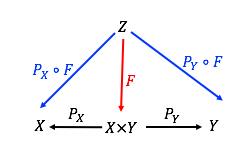
\includegraphics[width=6cm]{week3/p_3}
\caption{Diagram summarizing the statement~(*)}
\end{figure}
namely,
\begin{quotation}
\textit{
the mapping $F:Z\to X\times Y$ is continuous iff both $P_X\circ F:Z\to X$ and $P_Y\circ F:Z\to Y$ are continuous}. (*)
\end{quotation}
\end{enumerate}
\end{proposition}
\begin{proof}
\begin{enumerate}
\item
For any open $U$, we imply $p_X^{-1}(U)=U\times Y\in\mathcal{B}_{X\times Y}\subseteq\mathcal{T}_{X\times Y}$, i.e., $p_X^{-1}(U)$ is open. The same goes for $p_Y$.
\item
It suffices to show any topology $\mathcal{T}$ that meets the condition in (2) must contain $\mathcal{T}_{\text{product}}$. We imply that for $\forall U\in\mathcal{T}_X,V\in\mathcal{T}_Y$, 
\[
\left\{
\begin{aligned}
p_X^{-1}(U)&=U\times X\in\mathcal{T}\\
p_Y^{-1}(V)&=X\times V\in\mathcal{T}
\end{aligned}
\right.
\implies
(U\times Y)\cap(X\times V)=(U\cap X)\times (Y\cap V)=U\times V\in\mathcal{T},
\]
which implies $\mathcal{B}_{X\times Y}\subseteq\mathcal{T}$. Since $\mathcal{T}$ is closed for union operation on subsets, we imply $\mathcal{T}_{\text{product topology}}\subseteq\mathcal{T}$.
\item
\begin{enumerate}
\item
Firstly show that $\mathcal{T}_{\text{product}}$ satisfies (*).
\begin{itemize}
\item
For the forward direction, by (1) we imply both $p_X\circ F$ and $p_Y\circ F$ are continuous, since the composition of continuous functions are continuous as well.
\item
For the reverse direction, for $\forall U\times\mathcal{T}_X,V\in\mathcal{T}_Y$,
\[
F^{-1}(U\times V)=(p_X\circ F)^{-1}(X)\cap (p_Y\circ F)^{-1}(Y),
\]
which is open due to the continuity of $p_X\circ F$ and $p_Y\circ F$.
\end{itemize}
\item
Then we show the uniqueness of $\mathcal{T}_{\text{product}}$. Let $\mathcal{T}$ be another topology $X\times Y$ satisfying (*).
\begin{itemize}
\item
Take $Z=(X\times Y,\mathcal{T})$, and consider the identity mapping $F=\text{id}:Z\to Z$, which is continuous. Therefore $p_X\circ\text{id}$ and $p_Y\circ\text{id}$ are continuous, i.e., $p_X$ and $p_Y$ are continuous. By (2) we imply $\mathcal{T}_{\text{product}}\subseteq\mathcal{T}$.
\item
Take $Z=(X\times Y,\mathcal{T}_{\text{product}})$, and consider the identity mapping $F=\text{id}:Z\to Z$. Note that $p_X\circ F=p_X$ and $p_Y\circ F=p_Y$, which is continuous by (1). Therefore, the identity mapping $F:(X\times Y,\mathcal{T}_{\text{product}})\to(X\times Y,\mathcal{T})$ is continuous, which implies
\[
U=\text{id}^{-1}(U)\subseteq\mathcal{T}_{\text{product}}\ \text{for }\forall U\in\mathcal{T},
\]
i.e., $\mathcal{T}\subseteq\mathcal{T}_{\text{product}}.$
\end{itemize}
The proof is complete.
\end{enumerate}


\end{enumerate}
\end{proof}

\begin{definition}[Disjoint Union]
Let $X\times Y$ be two topological spaces, then the \emph{disjoint union} of $X$ and $Y$ is
\[
X\coprod Y:=(X\times\{0\})\cup(Y\times\{1\})
\]
\end{definition}
\begin{remark}
\begin{enumerate}
\item
We define that $U$ is open in $X\coprod Y$ if
\begin{enumerate}
\item
$U\cap(X\times\{0\})$ is open in $X\times\{0\}$; and
\item
$U\cap(Y\times\{1\})$ is open in $Y\times\{1\}$.
\end{enumerate}
We also need to show the well-definedness for this definition.
\item
$S$ is open in $X\coprod Y$ iff $S$ can be expressed as
\[
S=(U\times\{0\})\cup(V\times\{1\})
\]
where $U\subseteq X$ is open and $V\subseteq Y$ is open.
\end{enumerate}
\end{remark}


\subsection{Properties of Topological Spaces}
\subsubsection{Hausdorff Property}
\begin{definition}[First Separation Axiom]
A topological space $X$ satisfies the \emph{first separation axiom} if for any two distinct points $x\ne y\in X$, there exists open $U\ni x$ but not including $y$.
\end{definition}

\begin{proposition}
A topological space $X$ has first separation property if and only if for $\forall x\in X$, $\{x\}$ is closed in $X$.
\end{proposition}
\begin{proof}
\textit{Sufficiency.}
Suppose that $x\ne y$, then construct $U:=X\setminus\{y\}$, which is a open set that contains $x$ but not includes $y$.

\textit{Necessity.}
Take any $x\in X$, then for $\forall y\ne x$, there exists $y\in U_y$ that is open and $x\notin U_y$. Thus 
\[
\{y\}\subseteq U_y\subseteq X\setminus\{x\}
\]
which implies
\[
\bigcup_{y\in X\setminus\{x\}}\{y\}\subseteq
\bigcup_{y\in X\setminus\{x\}}U_y\subseteq
X\setminus\{x\},
\]
i.e., $X\setminus\{x\}=\bigcup_{y\in X\setminus\{x\}}U_y$ is open in $X$, i.e., $\{x\}$ is closed in $X.$
\end{proof}

\begin{definition}[Second separation Axiom]
A topological space satisfies the \emph{second separation axiom} (or $X$ is Hausdorff) if for all $x\ne y$ in $X$, there exists open sets $U,V$ such that
\[
\begin{array}{lll}
x\in U,
&
y\in V,
&
U\cap V=\emptyset
\end{array}
\]
\end{definition}

\begin{example}
All metrizable topological spaces are Hausdorff.

Suppose $d(x,y)=r>0$, then take $B_{r/2}(x)$ and $B_{r/2}(y)$
\end{example}

\begin{example}
Note that a topological space that is \emph{first separable} may not necessarily be \emph{second separable}:

Consider $\mathcal{T}_{\text{co-finite}}$, then $X$ is first separable but not Hausdorff:

Suppose on the contrary that for given $x\ne y$, there exists open sets $U,V$ such that $x\in U,y\in V$, and
\[
U\cap V=\emptyset\implies
X = X\setminus (U\cap V) = (X\setminus U)\cup(X\setminus V),
\]
implying that the union of two finite sets equals $X$, which is infinite, which is a contradiction.
\end{example}



















\chapter{Week4}
\section{Monday for MAT3040}\index{Monday_lecture}

\subsection{Quotient Spaces}

Now we aim to divide a big \emph{vector space} into many pieces of slices. 
\begin{itemize}
\item
For example, the Cartesian plane can be expressed as union of set of vertical lines as follows:
\[
\mathbb{R}^2 = \bigcup_{m\in\mathbb{R}}\left\{\begin{pmatrix}
m\\0
\end{pmatrix}+
\Span\{(0,1)\}\}
\right\}
\]
\item
Another example is that the set of integers can be expressed as union of three sets:
\[
\mathbb{Z}
=
Z_1\cup Z_2\cup Z_3,
\]
where $Z_i$ is the set of integers $z$ such that $z\text{ mod }3 = i$.
\end{itemize}

\begin{definition}[Coset]
Let $V$ be a vector space and $W\le V$. For any element $\bm v\in V$, the \emph{(right) coset} determined by $\bm v$ is the set
\[
\bm v+W:=\{\bm v+\bm w\mid\bm w\in W\}
\]
\end{definition}

For example, consider $V=\mathbb{R}^3$ and $W=\Span\{(1,2,0)\}$. Then the coset determined by $\bm v=(5,6,-3)$ can be written as
\[
\bm v+W=\left\{(5+t,6+2t,-3)\mid t\in\mathbb{R}\right\}
\]
It's interesting that the coset determined by $\bm v'=\{(4,4,-3)\}$ is exactly the same as the coset shown above:
\[
\bm v'+W=\left\{(4+t,4+2t,-3)\mid t\in\mathbb{R}\right\}=\bm v+W.
\]

Therefore, write the exact expression of $\bm v+W$ may sometimes become tedious and hard to check the equivalence. We say $\bm v$ is a \emph{representative} of a coset $\bm v+W$.

\begin{proposition}\label{pro:4:1}
Two cosets are the same iff the subtraction for the corresponding representatives is in $W$, i.e., 
\[
\bm v_1+W=\bm v_2+W
\Longleftrightarrow
\bm v_1-\bm v_2\in W
\]
\end{proposition}
\begin{proof}
\textit{Necessity.}
Suppose that $\bm v_1+W=\bm v_2+W$, then $\bm v_1+\bm w_1=\bm v_2+\bm w_2$ for some $\bm w_1,\bm w_2\in W$, which implies
\[
\bm v_1-\bm v_2=\bm w_2-\bm w_1\in W
\]
\textit{Sufficiency.}
Suppose that $\bm v_1-\bm v_2=\bm w\in W$. It suffices to show $\bm v_1+W\subseteq\bm v_2+W$.
For any $\bm v_1+\bm w'\in \bm v_1+W$, this element can be expressed as
\[
\bm v_1+\bm w'=(\bm v_2+\bm w)+\bm w'=\bm v_2+\underbrace{(\bm w+\bm w')}_{\text{belong to $W$}}\in \bm v_2+W.
\]
Therefore, $\bm v_1+W\subseteq \bm v_2+W$. Similarly we can show that $\bm v_2+W\subseteq \bm v_1+W$.
\end{proof}
\textit{Exercise: }Two cosets with representatives $\bm v_1,\bm v_2$ have no intersection iff $\bm v_1-\bm v_2\notin W$.

\begin{definition}[Quotient Space]
The \emph{quotient space} of $V$ by the subspace $W$, is the collection of all cosets $\bm v+W$, denoted by $V/ W$.
\end{definition}
To make the quotient space a vector space structure, we define the addition and scalar multiplication on $V/ W$ by:
\begin{align*}
(\bm v_1+W)+(\bm v_2+W)&:=(\bm v_1+\bm v_2)+W\\
\alpha\cdot (\bm v+W)&:=(\alpha\cdot\bm v) + W
\end{align*}

For example, consider $V=\mathbb{R}^2$ and $W=\Span\{(0,1)\}$. Then note that
\begin{align*}
\left(
\begin{pmatrix}
1\\0
\end{pmatrix}+W
\right)
+
\left(
\begin{pmatrix}
2\\0
\end{pmatrix}+W
\right)
&=
\left(
\begin{pmatrix}
3\\0
\end{pmatrix}+W
\right)\\
\pi\cdot\left(
\begin{pmatrix}
1\\0
\end{pmatrix}+W
\right)
&=
\left(
\begin{pmatrix}
\pi\\0
\end{pmatrix}+W
\right)
\end{align*}

\begin{proposition}
The addition and scalar multiplication is well-defined.
\end{proposition}
\begin{proof}
\begin{enumerate}
\item
Suppose that
\begin{equation}\label{Eq:4:1}
\left\{
\begin{aligned}
\bm v_1+W&=\bm v_1'+W\\
\bm v_2+W&=\bm v_2'+W
\end{aligned}
\right.,
\end{equation}
and we need to show that $(\bm v_1+\bm v_2)+W=(\bm v_1'+\bm v_2')+W$. 

From (\ref{Eq:4:1}) and proposition~(\ref{pro:4:1}), we imply
\[
\bm v_1-\bm v_1'\in W,\quad
\bm v_2-\bm v_2'\in W
\]
which implies
\[
(\bm v_1-\bm v_1')+(\bm v_2-\bm v_2')=(\bm v_1+\bm v_2) - (\bm v_1'+\bm v_2')\in W
\]

By proposition~(\ref{pro:4:1}) again we imply $(\bm v_1+\bm v_2)+W=(\bm v_1'+\bm v_2')+W$
\item
For scalar multiplication, similarly, we can show that $\bm v_1+W=\bm v_1'+W$ implies $\alpha\bm v_1+W=\alpha\bm v_1'+W$ for all $\alpha\in\mathbb{F}$.

\end{enumerate}

\end{proof}

\begin{proposition}
The canonical projection mapping
\[
\begin{aligned}
\pi_W:&V\to V/ W,\\
&\bm v\mapsto\bm v+W,
\end{aligned}
\]
is a \emph{surjective} \emph{linear transformation} with $\ker(\pi_W) = W$.
\end{proposition}
\begin{proof}
\begin{enumerate}
\item
First we show that $\ker(\pi_W)=W$:
\[
\pi_W(\bm v)=0\implies
\bm v+W=\bm0_{V/ W}\implies
\bm v+W=\bm0+W\implies \bm v=(\bm v-\bm0)\in W
\]
Here note that the zero element in the quotient space $V/ W$ is the coset with representative $\bm0$.
\item
For any $\bm v_0+W\in V/ W$, we can construct $\bm v_0\in V$ such that $\pi_W(\bm v_0)=\bm v_0+W$. Therefore the mapping $\pi_W$ is surjective.
\item
To show the mapping $\pi_W$ is a linear transformation, note that
\begin{align*}
\pi_W(\alpha\bm v_1+\beta\bm v_2)&=(\alpha\bm v_1+\beta\bm v_2)+W\\
&=(\alpha\bm v_1+W)+(\beta\bm v_2+W)\\
&=\alpha(\bm v_1+W)+\beta(\bm v_2+W)\\
&=\alpha\pi_W(\bm v_1)+\beta\pi_W(\bm v_2)
\end{align*}

\end{enumerate}


\end{proof}



\subsection{First Isomorphism Theorem}
The key of linear algebra is to solve the linear system $\bm A\bm x=\bm b$ with $\bm A\in\mathbb{R}^{m\times n}$. 
The general step for solving this linear system is as follows:
\begin{enumerate}
\item
Find the solution set for $\bm A\bm x=\bm0$, i.e., the set $\ker(\bm A)$
\item
Find a particular solution $\bm x_0$ such that $\bm A\bm x_0=\bm b$.
\end{enumerate}
Then the general solution set to this linear system is $\bm x_0+\ker(\bm A)$, which is a coset in the space $\mathbb{R}^n/ \ker(\bm A)$. Therefore, to solve the linear system $\bm{Ax}=\bm b$ suffices to study the quotient space $\mathbb{R}^n/ \ker(\bm A)$:

\begin{proposition}[Universal Property I]
Suppose that $T:V\to W$ is a linear transformation, and that $V'\le\ker(T)$. Then the mapping
\begin{align*}
\tilde{T}&:V/ V'\to W\\
&\bm v+V'\mapsto T(\bm v)
\end{align*}
is a well-defined linear transformation. As a result, the diagram below commutes:
\begin{figure}[H]
\centering
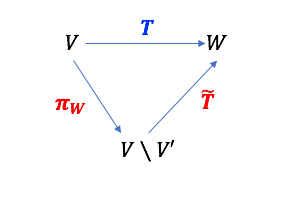
\includegraphics[width=0.5\textwidth]{week4/p_1}
\end{figure}
In other words, we have $T = \tilde{T}\circ \pi_W$.
\end{proposition}

\begin{proof}
First we show the well-definedness. Suppose that $\bm v_1+V'=\bm v_2+V'$ and suffices to show $\tilde T(\bm v_1+V')=\tilde T(\bm v_2+V')$, i.e., $T(\bm v_1)=T(\bm v_2)$. By proposition~(\ref{pro:4:1}), we imply
\[
\bm v_1-\bm v_2\in V'\le\ker(T)\implies
T(\bm v_1-\bm v_2)=\bm0\implies T(\bm v_1)-T(\bm v_2)=\bm0.
\]
Then we show $\tilde(T)$ is a linear transformation:
\begin{align*}
\tilde{T}(\alpha(\bm v_1+V')  + \beta(\bm v_2+V'))&=\tilde{T}((\alpha\bm v_1+\beta\bm v_2)+V')\\
&=T(\alpha\bm v_1+\beta\bm v_2)\\
&=\alpha T(\bm v_1)+\beta T(\bm v_2)\\
&=\alpha\tilde{T}(\bm v_1+V')+\beta\tilde{T}(\bm v_2+V')
\end{align*}
\end{proof}

Actually, if we let $V'=\ker(T)$, the mapping $\tilde{T}:V/ V'\to T(V)$ forms an isomorphism, In particular, if further $T$ is surjective, then $T(V)=W$, i.e., the mapping $\tilde{T}:V/ V'\to W$ forms an isomorphism.
\begin{theorem}[First Isomorphism Theorem]
Let $T:V\to W$ be a surjective linear transformation. Then the mapping 
\begin{align*}
\tilde{T}&:V/ \ker(T)\to W\\
&\bm v+\ker(T)\mapsto T(\bm v)
\end{align*}
is an isomorphism.
\end{theorem}
\begin{proof}
\textit{Injectivity.} Suppose that $\tilde{T}(\bm v_1+\ker(T)) = \tilde{T}(\bm v_2+\ker(T))$, then we imply
\[
T(\bm v_1)=T(\bm v_2)\implies T(\bm v_1-\bm v_2)=\bm0_W\implies\bm v_1-\bm v_2\in\ker(T),
\]
i.e., $\bm v_1+\ker(T)=\bm v_2+\ker(T)$.

\textit{Surjectivity.} For $\bm w\in W$, due to the surjectivity of $T$, we can find a $\bm v_0$ such that $T(\bm v_0)=\bm w$. Therefore, we can construct a set $\bm v_0+\ker(T)$ such that
\[
\tilde{T}(\bm v_0+\ker(T))=\bm w.
\]
\end{proof}




















\section{Monday for MAT3006}\index{Monday_lecture}
\subsection{Remarks on MCT}
\begin{example}
The MCT can help us to compute the integral
\begin{align*}
\lim_{n\to\infty}\int_{[0,n\pi]}\cos\left(\frac{x}{2n}\right)xe^{-x^2}\diff x
\end{align*}

Construct $f_n(x) = \cos\left(\frac{x}{2n}\right)xe^{-x^2}\mathcal{X}_{[0,n\pi]}$.
\begin{itemize}
\item
Since $\cos(x/2n)<\cos(x/2(n+1))$ for any $x\in[0,n\pi]$, we imply $f_n$ is monotone increasing with $n$
\item
$f_n(x)$ is integrable for all $n$.
\item
$f_n$ converges pointwise to $xe^{-x^2}\mathcal{X}_{[0,\infty)}$
\end{itemize}
Therefore, MCT I applies and
\[
\lim_{n\to\infty}\int_{[0,n\pi]}\cos\left(\frac{x}{2n}\right)xe^{-x^2}\diff x
=
\int\left(\lim_{n\to\infty}f_n\right)\diff m
\]
with
\[
\lim_{n\to\infty}f_n = xe^{-x^2}\mathcal{X}_{[0,\infty)}.
\]
Moreover, 
\begin{subequations}
\begin{align}
\int\left(\lim_{n\to\infty}f_n\right)\diff m &= 
\lim_{m\to\infty}\int_{[0,m]}xe^{-x^2}\diff x\label{Eq:12:1}\\
&=\int_0^\infty xe^{-x^2}\diff x\\
&=\frac{1}{2}
\end{align}
where (\ref{Eq:12:1}) is by applying MCT I with $g_m(x) = xe^{-x^2}\mathcal{X}_{[0,m]}$ and proposition~(\ref{pro:10:14}) to compute a Lebesgue integral by evaluating a proper Riemann integral.
\end{subequations}
\end{example}

Then we discuss the Lebesgue integral for series:

\begin{corollary}[Lebesgue Series Theorem]
Let $\{f_n\}$ be a series of measurable functions such that
\[
\sum_{n=1}^\infty\int|f_n|\diff m<\infty,
\]
then $\sum_{n=1}^kf_n$ converges to an integrable function $f = \sum_{n=1}^\infty f_n$ a.e., with
\[
\int f\diff m = \sum_{n=1}^\infty\int f_n\diff m
\]
\end{corollary}
\begin{proof}
\begin{itemize}
\item
For each $f_n$, consider 
\[
f_n = f_n^+ - f_n^-,\ \text{where $f_n^+,f_n^-$ are nonnegative}.
\]
By proposition~(\ref{pro:11:6}), 
\[
\int\sum_{n=1}^\infty f_n^+\diff m = \sum_{n=1}^\infty\int f_n^+\diff m\le \sum_{n=1}^\infty\int |f_n|\diff m<\infty.
\]
Therefore, $f^+:=\sum_{n=1}^\infty f_n^+=\lim_{k\to\infty}\sum_{n=1}^kf_n^+$ is integrable.
The same follows by replacing $f^{+}$ with $f^{-}$.
By corollary~(\ref{cor:9:6}), $f^+(x),f^-(x)<\infty,\forall x\in U$, where $U^c$ is null.
\item
Therefore, construct 
\[
f(x)=\left\{
\begin{aligned}
f^+(x)-f^-(x),&\quad x\in U\\
0,&\quad x\in U^c
\end{aligned}
\right.
\]
Moreover, for $x\in U$, 
\begin{align*}
f(x)&=\left(\lim_{k\to\infty}\sum_{n=1}^kf_n^+(x)\right)-
\left(\lim_{k\to\infty}\sum_{n=1}^kf_n^-(x)\right)\\
&=\lim_{k\to\infty}
\left(
\sum_{n=1}^kf_n^+(x)
-
\sum_{n=1}^kf_n^-(x)
\right)\\
&=\lim_{k\to\infty}\left[\sum_{n=1}^k(f_n^+(x)-f_n^-(x))\right]
\\&=
\sum_{n=1}^\infty f_n(x)
\end{align*}
where the first equality is because that both terms are finite.
\item
It follows that
\begin{subequations}
\begin{align}
\int f\diff m&=\int f^+\diff m - \int f^-\diff m\label{Eq:12:2:a}\\
&=
\int\sum_{n=1}^\infty f_n^+\diff m -\int\sum_{n=1}^\infty f_n^-\diff m\\
&=\left(\sum_{n=1}^\infty\int f_n^+\diff m\right)
-
\left(\sum_{n=1}^\infty\int f_n^-\diff m\right)\label{Eq:12:2:c}\\
&=\sum_{n=1}^\infty
\left(
\int f_n^+\diff m -\int f_n^-\diff m
\right)\label{Eq:12:2:d}\\
&=\sum_{n=1}^\infty\int f_n\diff m\label{Eq:12:2:e}
\end{align}
where (\ref{Eq:12:2:a}),(\ref{Eq:12:2:d}) is because that summation/subtraction between series holds when these series are finite; (\ref{Eq:12:2:c}) is by proposition~(\ref{pro:11:6}); (\ref{Eq:12:2:e}) is by definition of $f_n$.
\end{subequations}
\end{itemize}
\end{proof}

\begin{example}
Compute the integral
\[
\int_{(0,1]}e^{-x}x^{\alpha-1}\diff x,\ \alpha>0.
\]
\begin{itemize}
\item
Construct $f_n(x) = (-1)^n\frac{x^{\alpha+n-1}}{n!}\mathcal{X}_{(0,1]}, n\ge0$, and
\[
\sum_{n=0}^N f_n(x)\to e^{-x}x^{\alpha-1}, \ \text{pointwisely}, x\in(0,1]. 
\]
By applying MCT I,
\[
\int|f_n|\diff m=\frac{1}{(\alpha+n)n!}
\]
Therefore, 
\[
\sum_{n=0}^\infty\int|f_n|\diff m=
\sum_{n=0}^\infty\frac{1}{(\alpha+n)n!}<\infty
\]
\item
Applying the Lebesgue Series Theorem,
\[
\int_{(0,1]}e^{-x}x^{\alpha-1}\diff x = 
\int_{(0,1]}(\sum_{n=0}^\infty f_n)\diff m
=
\sum_{n=0}^\infty\int f_n\diff m=
\sum_{n=0}^\infty\frac{(-1)^n}{(\alpha+n)n!}
\]
\end{itemize}
\end{example}

\begin{remark}
It's essential to have $\sum\int|f|\diff m<\infty$ rather than $\sum\int f_n\diff m<\infty$ in the Lebesgue Series Theorem.
For example, let
\[
f_n=\frac{(-1)^{n+1}}{(n+1)}\mathcal{X}_{[n,n+1)}
\implies
\sum_{n=1}^\infty\int f_n\diff m =\log(2)<\infty
\]
However, $f:=\sum f_n$ is not integrable.
\end{remark}

\subsection{Dominated Convergence Theorem}
\begin{theorem}
Let $\{f_n\}$ be a sequence of measruable functions such that $|f_n|\le g$ a.e., and $g$ is integrable.
Suppose that $\lim_{n\to\infty}f_n(x)=f(x)$ a.e., then
\begin{enumerate}
\item
$f$ is integrable,
\item
\[
\int f\diff m =\lim_{n\to\infty}\int f_n\diff m
\]
\end{enumerate}
\end{theorem}
\begin{proof}
\begin{itemize}
\item
Observe that 
\[
|f_n|\le g\implies
\lim_{n\to\infty}|f_n|\le g\implies |f|\le g
\]
By comparison test, $g$ is integrable implies $|f|$ is integrable, and further $f$ is integrable.
\item
Consider the sequence of non-negative functions
$\{g-f_n\}_{n\in\mathbb{N}}$ and $\{g+f_n\}_{n\in\mathbb{N}}$.

By Fatou's Lemma, 
\begin{align*}
\lim_{n\to\infty}\inf\int(g-f_n)\diff m&\ge \int \lim_{n\to\infty}\inf(g-f_n)\diff m\\
&=\int(g-f)\diff m\\
&=\int g\diff m - \int f\diff m
\end{align*}
which follows that
\[
\int g\diff m - \lim_{n\to\infty}\sup\int f_n\diff m
\ge
\int g\diff m - \int f\diff m
\]
i.e.,
\[
\int f\diff m\ge  \lim_{n\to\infty}\sup\int f_n\diff m
\]
\item
Similarly, 
\[
\lim_{n\to\infty}\inf(g+f_n)\diff m\ge \int\lim_{n\to\infty}\inf(g+f_n)\diff m
=
\int g\diff m + \int f\diff m
\]
which implies
\[
 \lim_{n\to\infty}\inf\int f_n\diff m\ge\int f\diff m
\]
\end{itemize}
As a result,
\[
 \lim_{n\to\infty}\sup\int f_n\diff m
 \le
 \int f\diff m\le  \lim_{n\to\infty}\inf\int f_n\diff m,
\]
which implies
\[
\int f\diff m = \lim_n\int f_n\diff m
\]
\end{proof}

\begin{corollary}[Bounded Convergence Theorem]
Suppose that $E\in\mathcal{M}$ be such that $m(E)<\infty$.
If
\begin{itemize}
\item
$|f_n(x)|\le K<\infty$ for any $x\in E,n\in\mathbb{N}$
\item
$f_n\to f$ a.e. in $E$,
\end{itemize}
then $f$ is integrable in $E$ with
\[
\int_Ef\diff m = \lim_{n\to\infty}\int f_n\diff m
\]
\end{corollary}
\begin{proof}
Take $g=K\mathcal{X}_E$ in DCT.
\end{proof}


\begin{proposition}
Every Riemann integrable function $f$ on $[a,b]$ is Lebesgue integrable, without the condition that $f$ is continuous a.e.
\end{proposition}
\begin{proof}
Since $f$ is Riemann integrable, we imply $f$ is bounded.
We construct the Riemann lower abd upper functions with $2^n$ equal intervals, denoted as $\{\phi_n\}$ and $\{\psi_n\}$, which follows that
\begin{itemize}
\item
$\phi_n$ is monotone increasing;
$\psi_n$ is monotone decreasing;
\item
$\phi_n\le f\le \psi_n$, and
\[
\lim_{n\to\infty}\int_{[a,b]}\phi_n=\int_a^bf(x)\diff x = \lim_{n\to\infty}\int_{[a,b]}\psi_n.
\]
\end{itemize}
Construct $g=\sup_n\phi_n$ and $h=\inf_n\psi_n$.
Now we can apply the bounded convergence theorem:
\begin{itemize}
\item
$\phi_n$ is bounded on $[a,b]$
\item
$\phi_n\to g$ on $[a,b]$
\end{itemize}
which implies
$g$ is Lebesgue integrable on $[a,b]$, with 
\[
\int_{[a,b]}g\diff m = \lim_{n\to\infty}\int_{[a,b]}\phi_n\diff m=\int_a^bf(x)\diff x.
\]
Similarly, $h$ is Lebesgue integrable, with
\[
\int_{[a,b]}h\diff m = \lim_{n\to\infty}\int_{[a,b]}\psi_n\diff m=\int_a^bf(x)\diff x.
\]
Moreover, $g\le f\le h$, and
\[
\int_{[a,b]}(h-g)\diff m = \int_{[a,b]}h\diff m - \int_{[a,b]}g\diff m=\int_a^bf(x)\diff x-\int_a^bf(x)\diff x=0,
\]
which implies $h=g$ a.e., and further $f=g$ a.e., which implies
\[
\int_{[a,b]} f\diff m = \int_{[a,b]} g\diff m= \int_a^bf(x)\diff x.
\]
\end{proof}
\begin{remark}
However, an improper Riemann integral does not necessarily has the corresponding Lebesgue integral:
\[
f(x)=\sum_{n=1}^\infty (-1)^nn\cdot\mathcal{X}_{(1/(n+1),1/n]},\ x\in[0,1]
\]
In this case, $f$ is Riemann integrable but not Lebesgue integrable.
\end{remark}














\section{Monday for MAT4002}\index{Monday_lecture}

\paragraph{Reviewing}
\begin{enumerate}
\item
Topological Space $(X,\mathcal{J})$: a special class of topological space is that induced from metric space $(X,d)$:
\[
(X,\mathcal{T}),\quad\text{with }\mathcal{T}=\{\text{all open sets in $(X,d)$}\}
\]
\item
Closed Sets $(X\setminus U)$ with $U$ open.
\end{enumerate}

\begin{proposition}
Let $(X,\mathcal{T})$ be a topological space, 
\begin{enumerate}
\item
$\emptyset, X$ are closed in $X$
\item
$V_1,V_2$ closed in $X$ implies that $V_1\bigcup V_2$ closed in $X$
\item
$\{V_\alpha\mid\alpha\in\mathcal{A}\}$ closed in $X$ implies that $\bigcap_{\alpha\in\mathcal{A}}V_\alpha$ closed in $X$
\end{enumerate}
\end{proposition}
\begin{proof}
Applying the De Morgan's Law
\[
(X\setminus\bigcup_{i\in I}U_i)=\bigcap_{i\in I}(X\setminus U_i)
\]
\end{proof}

\subsection{Convergence in topological space}

\begin{definition}[Convergence]
A sequence $\{x_n\}$ of a topological space $(X,\mathcal{T})$ converges to $x\in X$ 
if $\forall U\ni x$ is open, there $\exists N$ such that $x_n\in U,\forall n\ge N$.
\end{definition}

\begin{example}
\begin{enumerate}
\item
The topology for the space $(X=\mathbb{R}^n,d_2)\to(X,\mathcal{T})$ (i.e., a topological space induced from meric space $(X=\mathbb{R}^n,d_2)$) is called a \emph{usual topology} on $\mathbb{R}^n$.

When I say $\mathbb{R}^n$ (or subset of $\mathbb{R}^n$) is a topological space, 
it is equipeed with usual topology.

Convergence of sequence in $(\mathbb{R}^n,\mathcal{T})$ is the usual convergence in analysis.

For $\mathbb{R}^n$ or metric space, the limit of sequence (if exists) is unique.

\item

Consider the topological space $(X,\mathcal{T}_{\text{indiscrete}})$. 
Take any sequence $\{x_n\}$ in $X$, it is convergent to any $x\in X$. 
Indeed, for $\forall U\ni x$ open, $U=X$. Therefore, 
\[
x_n\in U(=X),\forall n\ge1.
\]
\item

Consider the topological space $(X,\mathcal{T}_{\text{cofinite}})$, where $X$ is infinite. 
Consider $\{x_n\}$ is a sequence satisfying $m\ne n$ implies $x_m\ne x_n$. 
Then $\{x_n\}$ is convergent to any $x\in X$.

(Question: how to define openness for $\mathcal{T}_{\text{cofinite}}$ and $\mathcal{T}_{\text{indiscrete}})$?
\item

Consider the topological space $(X,\mathcal{T}_{\text{discrete}})$, 
the sequence $\{x_n\}\to x$ is equivalent to say $x_n=x$ for all sufficiently large $n$.
\end{enumerate}
\end{example}
\begin{remark}
The limit of sequences may not be unique. The reason is that ``$\mathcal{T}$ is not big enough''. We will give a criterion to make sure the limit is unique in the future. (Hausdorff)
\end{remark}
\begin{proposition}\label{pro:2:9}
If $F\subseteq(X,\mathcal{T})$ is closed, then for any convergent sequence $\{x_n\}$ in $F$, the limit(s) are also in $F$.
\end{proposition}

\begin{proof}
Let $\{x_n\}$ be a sequence in $F$ with limit $x\in X$. 
Suppose on the contrary that $x\notin F$ 
(i.e., $x\in X\setminus F$ that is open). 
There exists $N$ such that
\[
x_n\in X\setminus F,\forall n\ge N,
\]
i.e., $x_n\notin F$, which is a contradiction.
\end{proof}
\begin{remark}
The converse may not be true. If the $(X,\mathcal{T})$ is metrizable, the converse holds.

Counter-example: Consider the co-countable topological space $(X=\mathbb{R},\mathcal{T}_{\text{co-co}})$, where 
\[
\mathcal{T}_{\text{co-co}}=
\{U\mid X\setminus U\text{ is a countable set}\}
\bigcup\{\emptyset\},
\]
and $X$ is uncontable. 
Then note that $F=[0,1]\subsetneqq X$ is an un-countable set, and under co-countable topology, $F\supseteq \{x_n\}\to x$ implies $x_n=x\in F$ for all $n$.
It's clear that $X\setminus F\notin \mathcal{T}_{\text{co-co}}$, i.e., $F$ is not closed.
\end{remark}

\subsection{Interior, Closure, Boundary}
\begin{definition}\label{def:2:5}
Let $(X,\mathcal{T})$ be a topological space, and $A\subseteq X$ a subset.
\begin{enumerate}
\item
The \emph{interior} of $A$ is 
\[
A^\circ=\bigcup_{U\subseteq A,U\text{ is open}}U
\]
\item
The \emph{closure} of $A$ is
\[
\overline{A}=\bigcap_{A\subseteq V,V\text{ is closed}}V
\]
\end{enumerate}

If $\overline{A}=X$, we say that $A$ is dense in $X$.

The graph illustration of the definition above is as follows:
\begin{figure}[H]
        \begin{subfigure}[b]{0.3\textwidth}
                \centering
                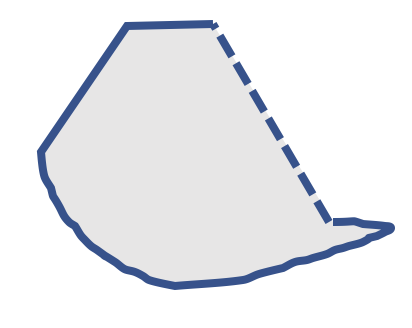
\includegraphics[width=\textwidth]{week2/p_1}
                \caption{Illustration of $A$}
                \label{fig:gull}
        \end{subfigure}%
        \begin{subfigure}[b]{0.3\textwidth}
                \centering
                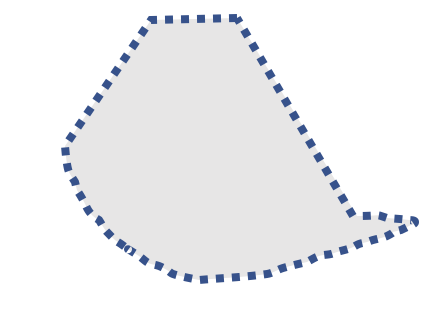
\includegraphics[width=\textwidth]{week2/p_2}
                \caption{Illustration of $A^\circ$}
                \label{fig:gull2}
        \end{subfigure}%
        \begin{subfigure}[b]{0.3\textwidth}
                \centering
                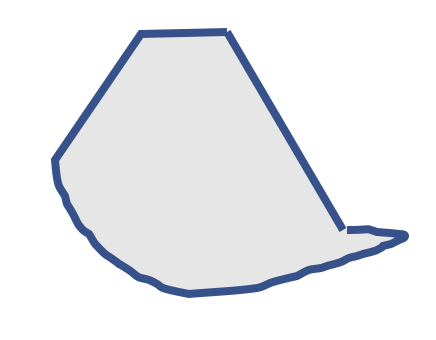
\includegraphics[width=\textwidth]{week2/p_3}
                \caption{Illustration of $\overline{A}$}
                \label{fig:tiger}
        \end{subfigure}
        \caption{Graph Illustrations}\label{fig:animals}
\end{figure}
\end{definition}
\begin{example}
\begin{enumerate}
\item

For $[a,b)\subseteq\mathbb{R}$, we have:
\[
\begin{array}{ll}
[a,b)^\circ=(a,b),
&
\overline{[a,b)}=[a,b]
\end{array}
\]

\item
For $X=\mathbb{R}$, $\mathbb{Q}^\circ=\emptyset$ and $\overline{\mathbb{Q}}=\mathbb{R}$.

\item
Consider the discrete topology $(X,\mathcal{T}_{\text{discrete}})$, we have
\[
\begin{array}{ll}
S^\circ=S,
&
\overline{S}=S
\end{array}
\]

\end{enumerate}
\end{example}

The insights behind the definition~(\ref{def:2:5}) is as follows

\begin{proposition}
\begin{enumerate}
\item
$A^\circ$ is the largest open subset of $X$ contained in $A$;

$\overline{A}$ is the smallest closed subset of $X$ containing $A$.
\item
If $A\subseteq B$, then $A^\circ\subseteq B$ and $\overline{A}\subseteq\overline{B}$
\item
$A$ is open in $X$ is equivalent to say $A^\circ = A$; $A$ is closed in $X$ is equivalent to say $\overline{A}=A$.
\end{enumerate}
\end{proposition}

\begin{example}
Let $(X,d)$ be a metric space. What's the closure of an open ball $B_r(x)$?

The direct intuition is to define the closed ball
\[
\bar B_r(x)=\{y\in X\mid d(x,y)\le r\}.
\]

Question: is $\bar B_r(x)=\overline{B_r(x)}$?
\begin{enumerate}
\item
Since $\bar B_r(x)$ is a closed subset of $X$, and 
$B_r(x)\subseteq \bar B_r(x)$, 
we imply that
\[
\overline{B_r(x)}\subseteq\bar B_r(x)
\]
\item
Howover, we may find an example such that $\overline{B_r(x)}$ is a proper subset of $\bar B_r(x)$:

Consider the discrete metric space $(X,d_{\text{discrete}})$ and for $\forall x\in X$,
\[
B_1(x)=\{x\}\implies
\overline{B_1(x)}=\{x\},\quad
\bar B_1(x)=X
\]

The equality $\bar B_r(x)=\overline{B_r(x)}$ holds when $(X,d)$ is a normed space.
\end{enumerate}
\end{example}

Here is another characterization of $\overline{A}$:

\begin{proposition}\label{pro:2:11}
\[
\overline{A}=\{x\in X\mid\forall \text{open }U\ni x, U\bigcap A\ne\emptyset\}
\]
\end{proposition}
\begin{proof}
Define
\[
S=\{x\in X\mid\forall \text{open }U\ni x, U\bigcap A\ne\emptyset\}
\]
It suffices to show that $\overline{A}=S$.
\begin{enumerate}
\item
First show that $S$ is closed:
\[
X\setminus S=\{x\in X\mid\exists U_x\ni x\text{ open s.t. }U_x\bigcap A=\emptyset\}
\]
Take $x\in X\setminus S$, we imply there exists open $U_x\ni x$ such that $U_x\bigcap A=\emptyset$. We claim $U_x\subseteq X\setminus S$:
\begin{itemize}
\item
For $\forall y\in U_x$, note that $U_x\ni y$ that is open, such that $U_x\bigcap A=\emptyset$. Therefore, $y\in X\setminus S$.
\end{itemize}

Therefore, we have $x\in U_x\subseteq X\setminus S$ for any $\forall x\in X\setminus S$.

Note that
\[
X\setminus S
=
\bigcup_{x\in X\setminus S}\{x\}\subseteq
\bigcup_{x\in X\setminus S}U_x\subseteq X\setminus S,
\]
which implies $X\setminus S=\bigcup_{x\in X\setminus S}U_x$ is open, i.e., $S$ is closed in $X$.
\item
By definition, it is clear that $A\subseteq S$:
\[
\forall a\in A,\forall\text{open }U\ni a,
U\bigcap A\supseteq\{a\}\ne\emptyset\implies a\in S.
\]
Therefore, $\overline{A}\subseteq\overline{S}=S$.
\item
Suppose on the contrary that 
there exists $y\in S\setminus\overline{A}$. 

Since $y\notin\overline{A}$, by definition, 
there exists $F\supseteq A$ closed such that 
$y\notin F$. 

Therefore, $y\in X\setminus F$ that is open, and 
\[
(X\setminus F)\bigcap A\subseteq(X\setminus A)\bigcap A=\emptyset\implies y\notin S,
\]
which is a contradiction. Therefore, $S=\overline{A}$.
\end{enumerate}
\end{proof}
\begin{definition}[accumulation point]
Let $A\subseteq X$ be a subset in a topological space. 
We call $x\in X$ are an 
\emph{accumulation point} (\emph{limit point}) of $A$ 
if
\[
\forall U\subseteq X\text{ open s.t. }
U\ni x, 
(U\setminus\{x\})\bigcap A\ne\emptyset.
\]

The set of accumulation points of $A$ is denoted as $A'$
\end{definition}
\begin{proposition}
$\overline{A}=A\bigcup A'$.
\end{proposition}

\begin{proof}
This proposition directly follows from Proposition~(\ref{pro:2:11}) and the definition of A'.
\end{proof}













\section{Wednesday for MAT3040}\index{Wednesday_lecture}
\subsection{Tensor Product for Linear Transformations}

\begin{proposition}
Suppose that $T:V\to V'$ and $S:W\to W'$ are linear transformations, then there exists an unique linear transformation 
\[
\begin{array}{ll}
T\otimes S:&V\otimes W\to V'\otimes W'\\
\text{satisfying}&(T\otimes S)(v\otimes w) = T(v)\otimes S(w)
\end{array}
\]
\end{proposition}

\begin{proof}
We construct the mapping
\[
\begin{array}{ll}
T\times S:&V\times W\to V'\otimes W'\\
\text{with}&(T\times S)(v,w) = T(v)\otimes S(w)
\end{array}
\]
This mapping is indeed bilinear: for instance, we can show that 
\[
(T\times S)(av_1+bv_2,w) = a(T\times S)(v_1,w)+b(T\times S)(v_2,w)
\]
Therefore, $T\times S\in\text{Obj}$. Since the tensor product satisfies the universal property, we imply there exists an unique linear transformation
\[
\begin{array}{ll}
T\otimes S&V\otimes W\to V'\otimes W'\\
\text{satisfying}&(T\otimes S)(v\otimes w)=T(v)\otimes S(w)
\end{array}
\]


\end{proof}
\paragraph{Notation Warning}
Does the notion $T\otimes S$ really form a tensor product, i.e., do we obtain the addictive rules for tensor product such as 
\[
(aT_1+bT_2)\otimes S = a(T_1\otimes S)+b(T_2\otimes S)?
\]


\begin{example}\label{exp:13:2}
Let $V=V'=\mathbb{F}^2$ and $W=W'=\mathbb{F}^3$.
Define the matrix-multiply mappings:
\[\left\{
\begin{array}{ll}
T:&V\to V\\
\text{with}&\bm v\mapsto\bm A\bm v\\
&\bm A=\begin{pmatrix}
a&b\\c&d
\end{pmatrix}
\end{array}\right.\qquad
\left\{
\begin{array}{ll}
S:&W\to W\\
\text{with}&\bm w\mapsto\bm B\bm w\\
&\bm B=\begin{pmatrix}
p&q&r\\
s&t&u\\
v&w&x
\end{pmatrix}
\end{array}
\right.
\]
How does $T\otimes S:V\otimes W\to V\otimes W$ look like?
\begin{itemize}
\item
Suppose $\{e_1,e_2\},\{f_1,f_2,f_3\}$ are usual basis of $V,W$, respectively.
Then the basis of $V\otimes W$ is given by:
\[
\mathcal{C}=\{e_1\otimes f_1,e_1\otimes f_2,e_1\otimes f_3,e_2\otimes f_1,e_2\otimes f_2,e_2\otimes f_3\}.
\]
\item
As a result, we can compute $(T\otimes S)(e_i\otimes f_j)$ for $i=1,2$ and $j=1,2,3$. For instance,
\begin{align*}
(T\otimes S)(e_1\otimes e_1)&=T(e_1)\otimes S(e_1)\\
&=(ae_1+ce_2)\otimes(pe_1+se_2+ve_3)\\
&=
(ap)e_1\otimes e_1+(as)e_1\otimes e_2+(av)e_1\otimes e_3+(cp)e_2\otimes e_1+(cs)e_2\otimes e_2+(cv)e_2\otimes e_3
\end{align*}
\item
Therefore, we obtain a matrix representation for the linear transformation $(T\otimes S)$:

\end{itemize}
We want a matrix representation for $(T\otimes S)$:
\[
(T\otimes S)_{\mathcal{C},\mathcal{C}}
=
\begin{pmatrix}
aB&bB\\
cB&dB
\end{pmatrix},
\]
which is a large matrix formed by taking all possible products between the elements of $\bm A$ and those of $\bm B$.
This operation is called the \emph{Kronecker Tensor Product}, see the command \textit{kron} in MATLAB for detail.


\end{example}
\begin{proposition}
More generally, given the linear operator $T:V\to V$ and $S:W\to W$, 
let $\mathcal{A}=\{v_1,\dots,v_n\},\mathcal{B}=\{w_1,\dots,w_m\}$ be a basis of $V,W$ respectively, with
\[
\begin{array}{ll}
(T)_{\mathcal{A},\mathcal{A}}=(a_{ij})
&
(S_{\mathcal{B},\mathcal{B}})=(b_{ij}):=B
\end{array}
\]
As a result, $(T\otimes S)_{\mathcal{C},\mathcal{C}}=A\otimes B$, where 
$\mathcal{C}=\{v_1\otimes w_1,\dots, v_n\otimes w_m\}$, and $A\otimes B$ denotes the Kronecker tensor product, defined as the matrix
\[
\begin{pmatrix}
a_{1,1}B&\cdots&a_{1,n}B\\
\vdots&\ddots&\vdots\\
a_{n,1}B&\cdots&a_{n,n}B
\end{pmatrix}.
\]
\end{proposition}
\begin{proof}
Following the similar procedure as in Example~(\ref{exp:13:2}) and applying the relation
\begin{align*}
(T\otimes S)(v_i\otimes w_j)&=T(v_i)\otimes S(w_j)\\
&=\left(
\sum_{k=1}^na_{ki}v_k
\right)
\otimes
\left(
\sum_{\ell=1}^mb_{\ell j}w_\ell
\right)\\
&=\sum_{k=1}^n\sum_{\ell=1}^m(a_{ki}b_{\ell j})v_k\otimes w_{\ell}
\end{align*}
\end{proof}

\begin{proposition}
The operation $T\otimes S$ satisfies all the properties of tensor product.
For example,
\begin{align*}
(aT_1+bT_2)\otimes S &= a(T_1\otimes S)+b(T_2\otimes S)\\
T\otimes(cS_1+dS_2) &= c(T\otimes S_1)+d(T\otimes S_2)
\end{align*}
Therefore, the usage of the notion ``$\otimes$'' is justified for the definition of $T\otimes S$.
\end{proposition}
\begin{proof}[Proof using matrix multiplication]
For instance, consider the operation $(T+T')\otimes S$, with $(T)_{\mathcal{A},\mathcal{A}}=(a_{ij})$, $(T')_{\mathcal{A},\mathcal{A}}=(c_{ij}), (S)_{\mathcal{B},\mathcal{B}}=B$.

We compute its matrix representation directly:
\begin{align*}
((T+T')\otimes S)_{\mathcal{C},\mathcal{C}}
&=
(T+T')_{\mathcal{A},\mathcal{A}}\otimes (S)_{\mathcal{B},\mathcal{B}}\\
&=
[(T)_{\mathcal{A},\mathcal{A}}+(T')_{\mathcal{A},\mathcal{A}}]\otimes (S)_{\mathcal{B},\mathcal{B}}\\
&=
(T)_{\mathcal{A},\mathcal{A}}\otimes (S)_{\mathcal{B},\mathcal{B}}
+
(T')_{\mathcal{A},\mathcal{A}}\otimes (S)_{\mathcal{B},\mathcal{B}}
\end{align*}
where the last equality is by the addictive rule for kronecker product for matrices.
Therefore,
\[
((T+T')\otimes S)_{\mathcal{C},\mathcal{C}}=
(T\otimes S)_{\mathcal{C},\mathcal{C}} + 
(T'\otimes S)_{\mathcal{C},\mathcal{C}}
\implies
(T+T')\otimes S
=
T\otimes S+T'\otimes S
\]
\end{proof}
\begin{proof}[Proof using basis of $T\otimes S$]
Another way of the proof is by computing 
\[
((T+T')\otimes S)(v_i\otimes w_j),
\] 
where $\{v_i\otimes w_j\mid 1\le i\le n,1\le j\le m\}$ forms a basis of $(T+T')\otimes S$:
\begin{align*}
((T+T')\otimes S)(v_i\otimes w_j)
&=(T+T')(v_i)\otimes S(w_j)\\
&=(T(v_i)+T'(v_i))\otimes S(w_j)\\
&=T(v_i)\otimes S(w_j)+T'(v_i)\otimes S(w_j)\\
&=(T\otimes S)(v_i\otimes w_j)+(T'\otimes S)(v_i\otimes w_j)
\end{align*}
Since $((T+T')\otimes S)(v_i\otimes w_j)$ coincides with $(T\otimes S + T'\otimes S)(v_i\otimes w_j)$ for all basis vectors $v_i\otimes w_j\in\mathcal{C}$, we imply
\[
(T+T')\otimes S = T\otimes S+T'\otimes S
\]
\end{proof}


\begin{proposition}
Let $A,C$ be linear operators from $V$ to $V$, and $B,D$ be linear operators from $W$ to $W$, then
\[
(A\otimes B)\circ(C\otimes D)=(AC)\otimes(BD)
\]
\end{proposition}

\begin{proposition}
Define linear operators $A:V\to V$ and $B:W\to W$ with $\dim(V),\dim(W)<\infty$.
Then
\[
\det(A\otimes B) = (\det(A))^{\dim(W)}(\det(B))^{\dim(V)}
\]
\end{proposition}

\begin{corollary}
There exists a linear transformation 
\[
\begin{array}{ll}
\Phi:&
\text{Hom}(V,V)\otimes\text{Hom}(W,W)\to
\text{Hom}(V\otimes W,V\otimes W)\\
\text{with}&A\otimes B\mapsto A\otimes B
\end{array}
\]
where the input of $\Phi$ is the tensor product of linear transformations, and the output is the linear transformation.
\end{corollary}
\begin{proof}
Construct the mapping
\[
\begin{array}{ll}
\Phi&:
\text{Hom}(V,V)\times\text{Hom}(W,W)\to
\text{Hom}(V\otimes W,V\otimes W)\\
\text{with}&\Phi(A,B)=A\otimes B
\end{array}
\]
The $\Phi$ is indeed bilinear: for instance, 
\begin{align*}
\Phi(pA+qC,B)&=(pA+qC)\otimes B\\
&=p(A\otimes B)+q(C\otimes B)\\
&=p\Phi(A,B)+q\Phi(C,B)
\end{align*}
This corollary follows from the universal property of tensor product.
\end{proof}
\begin{remark}
If assuming that $\dim(V),\dim(W)<\infty$, we imply
\begin{align*}
\dim(\text{Input space of $\Phi$})&=\dim(\text{Hom}(V,V))\dim(\text{Hom}(W,W))\\
&=
[\dim(V)\dim(V)]
\cdot
[\dim(W)\dim(W)]
=
[\dim(V)\dim(W)]^2\\
&=[\dim(V\otimes W)]^2\\
&=\dim(\text{Hom}(V\otimes W,V\otimes W))\\
&=\dim(\text{Output space of $\Phi$})
\end{align*}
Therefore, is $\Phi$ is an isomorphism?
If so, then every linear operator $\alpha:V\otimes W\to V\otimes W$ can be expressed as
\[
\alpha = A_1\otimes B_1+\cdots+A_k\otimes B_k
\]
where $A_i:V\to V$ and $B_j:W\to W$.
\end{remark}











\section{Wednesday for MAT4002}\index{Monday_lecture}
\subsection{Remarks on product space} 
\paragraph{Reviewing}
\begin{itemize}
\item
Product Topology: For topological space $(X,\mathcal{T}_X)$ and $(Y,\mathcal{Y})$, define the basis
\[
\mathcal{B}_{X\times Y}=\{U\times V\mid U\in\mathcal{T}_X,V\in\mathcal{T}_Y\}
\]
and the family of union of subsets in $\mathcal{B}_{X\times Y}$ forms a product topology.
\end{itemize}
\begin{proposition}
a ring torus is homeomorphic to the Cartesian product of two circles, say $S^1\times S^1\cong T$.
\end{proposition}
 \begin{proof}
 Define a mapping $f:[0,2\pi]\times [0,2\pi]\to T$ as
 \[
 f(\theta,\phi)=\begin{pmatrix}
(R+r\cos\theta)\cos\phi,
&
(R+r\cos\theta)\sin\phi,
&
r\sin\theta
\end{pmatrix}
 \]
Define $i:T\to\mathbb{R}^3$, we imply
 \[
 i\circ f:[0,2\pi]\times[0,2\pi]\to\mathbb{R}^3\ \text{is continuous}
 \]
 Therefore we imply $f:[0,2\pi]\times [0,2\pi]\to T$ is continuous. Together with the condition that 
\[
\left\{
\begin{aligned}
f(0,y)&=f(2\pi,y)\\
f(x,0)&=f(x,2\pi)
\end{aligned}
\right.
\]
we imply the function $f:S^1\times S^1\to T$ is continuous.
We can also show it is bijective. We can also show $f^{-1}$ is continuous.
 \end{proof}
 
\begin{proposition}
\begin{enumerate}
\item
Let $X\times Y$ be endowed with product topology. 
The projection mappings defined as
\begin{align*}
p_X:&X\times Y\to X,\ \text{with }p_X(x,y) = x\\
p_Y:&X\times Y\to Y,\ \text{with }p_Y(x,y)=y
\end{align*}
are continuous.
\item
(an equivalent definition for product topology)
The product topology is the \emph{coarest topology} on $X\times Y$ such that $p_X$ and $p_Y$ are both continuous.
\item
(an equivalent definition for product topology)
Let $Z$ be a topological space, then the product topology is the unique topology that the red and the blue line in the diagram commutes:
\begin{figure}[H]
\centering
\includegraphics[width=6cm]{week3/p_3}
\caption{Diagram summarizing the statement~(*)}
\end{figure}
namely,
\begin{quotation}
\textit{
the mapping $F:Z\to X\times Y$ is continuous iff both $P_X\circ F:Z\to X$ and $P_Y\circ F:Z\to Y$ are continuous}. (*)
\end{quotation}
\end{enumerate}
\end{proposition}
\begin{proof}
\begin{enumerate}
\item
For any open $U$, we imply $p_X^{-1}(U)=U\times Y\in\mathcal{B}_{X\times Y}\subseteq\mathcal{T}_{X\times Y}$, i.e., $p_X^{-1}(U)$ is open. The same goes for $p_Y$.
\item
It suffices to show any topology $\mathcal{T}$ that meets the condition in (2) must contain $\mathcal{T}_{\text{product}}$. We imply that for $\forall U\in\mathcal{T}_X,V\in\mathcal{T}_Y$, 
\[
\left\{
\begin{aligned}
p_X^{-1}(U)&=U\times X\in\mathcal{T}\\
p_Y^{-1}(V)&=X\times V\in\mathcal{T}
\end{aligned}
\right.
\implies
(U\times Y)\cap(X\times V)=(U\cap X)\times (Y\cap V)=U\times V\in\mathcal{T},
\]
which implies $\mathcal{B}_{X\times Y}\subseteq\mathcal{T}$. Since $\mathcal{T}$ is closed for union operation on subsets, we imply $\mathcal{T}_{\text{product topology}}\subseteq\mathcal{T}$.
\item
\begin{enumerate}
\item
Firstly show that $\mathcal{T}_{\text{product}}$ satisfies (*).
\begin{itemize}
\item
For the forward direction, by (1) we imply both $p_X\circ F$ and $p_Y\circ F$ are continuous, since the composition of continuous functions are continuous as well.
\item
For the reverse direction, for $\forall U\times\mathcal{T}_X,V\in\mathcal{T}_Y$,
\[
F^{-1}(U\times V)=(p_X\circ F)^{-1}(X)\cap (p_Y\circ F)^{-1}(Y),
\]
which is open due to the continuity of $p_X\circ F$ and $p_Y\circ F$.
\end{itemize}
\item
Then we show the uniqueness of $\mathcal{T}_{\text{product}}$. Let $\mathcal{T}$ be another topology $X\times Y$ satisfying (*).
\begin{itemize}
\item
Take $Z=(X\times Y,\mathcal{T})$, and consider the identity mapping $F=\text{id}:Z\to Z$, which is continuous. Therefore $p_X\circ\text{id}$ and $p_Y\circ\text{id}$ are continuous, i.e., $p_X$ and $p_Y$ are continuous. By (2) we imply $\mathcal{T}_{\text{product}}\subseteq\mathcal{T}$.
\item
Take $Z=(X\times Y,\mathcal{T}_{\text{product}})$, and consider the identity mapping $F=\text{id}:Z\to Z$. Note that $p_X\circ F=p_X$ and $p_Y\circ F=p_Y$, which is continuous by (1). Therefore, the identity mapping $F:(X\times Y,\mathcal{T}_{\text{product}})\to(X\times Y,\mathcal{T})$ is continuous, which implies
\[
U=\text{id}^{-1}(U)\subseteq\mathcal{T}_{\text{product}}\ \text{for }\forall U\in\mathcal{T},
\]
i.e., $\mathcal{T}\subseteq\mathcal{T}_{\text{product}}.$
\end{itemize}
The proof is complete.
\end{enumerate}


\end{enumerate}
\end{proof}

\begin{definition}[Disjoint Union]
Let $X\times Y$ be two topological spaces, then the \emph{disjoint union} of $X$ and $Y$ is
\[
X\coprod Y:=(X\times\{0\})\cup(Y\times\{1\})
\]
\end{definition}
\begin{remark}
\begin{enumerate}
\item
We define that $U$ is open in $X\coprod Y$ if
\begin{enumerate}
\item
$U\cap(X\times\{0\})$ is open in $X\times\{0\}$; and
\item
$U\cap(Y\times\{1\})$ is open in $Y\times\{1\}$.
\end{enumerate}
We also need to show the well-definedness for this definition.
\item
$S$ is open in $X\coprod Y$ iff $S$ can be expressed as
\[
S=(U\times\{0\})\cup(V\times\{1\})
\]
where $U\subseteq X$ is open and $V\subseteq Y$ is open.
\end{enumerate}
\end{remark}


\subsection{Properties of Topological Spaces}
\subsubsection{Hausdorff Property}
\begin{definition}[First Separation Axiom]
A topological space $X$ satisfies the \emph{first separation axiom} if for any two distinct points $x\ne y\in X$, there exists open $U\ni x$ but not including $y$.
\end{definition}

\begin{proposition}
A topological space $X$ has first separation property if and only if for $\forall x\in X$, $\{x\}$ is closed in $X$.
\end{proposition}
\begin{proof}
\textit{Sufficiency.}
Suppose that $x\ne y$, then construct $U:=X\setminus\{y\}$, which is a open set that contains $x$ but not includes $y$.

\textit{Necessity.}
Take any $x\in X$, then for $\forall y\ne x$, there exists $y\in U_y$ that is open and $x\notin U_y$. Thus 
\[
\{y\}\subseteq U_y\subseteq X\setminus\{x\}
\]
which implies
\[
\bigcup_{y\in X\setminus\{x\}}\{y\}\subseteq
\bigcup_{y\in X\setminus\{x\}}U_y\subseteq
X\setminus\{x\},
\]
i.e., $X\setminus\{x\}=\bigcup_{y\in X\setminus\{x\}}U_y$ is open in $X$, i.e., $\{x\}$ is closed in $X.$
\end{proof}

\begin{definition}[Second separation Axiom]
A topological space satisfies the \emph{second separation axiom} (or $X$ is Hausdorff) if for all $x\ne y$ in $X$, there exists open sets $U,V$ such that
\[
\begin{array}{lll}
x\in U,
&
y\in V,
&
U\cap V=\emptyset
\end{array}
\]
\end{definition}

\begin{example}
All metrizable topological spaces are Hausdorff.

Suppose $d(x,y)=r>0$, then take $B_{r/2}(x)$ and $B_{r/2}(y)$
\end{example}

\begin{example}
Note that a topological space that is \emph{first separable} may not necessarily be \emph{second separable}:

Consider $\mathcal{T}_{\text{co-finite}}$, then $X$ is first separable but not Hausdorff:

Suppose on the contrary that for given $x\ne y$, there exists open sets $U,V$ such that $x\in U,y\in V$, and
\[
U\cap V=\emptyset\implies
X = X\setminus (U\cap V) = (X\setminus U)\cup(X\setminus V),
\]
implying that the union of two finite sets equals $X$, which is infinite, which is a contradiction.
\end{example}



















%\chapter{Week4}
\section{Monday for MAT3040}\index{Monday_lecture}

\subsection{Quotient Spaces}

Now we aim to divide a big \emph{vector space} into many pieces of slices. 
\begin{itemize}
\item
For example, the Cartesian plane can be expressed as union of set of vertical lines as follows:
\[
\mathbb{R}^2 = \bigcup_{m\in\mathbb{R}}\left\{\begin{pmatrix}
m\\0
\end{pmatrix}+
\Span\{(0,1)\}\}
\right\}
\]
\item
Another example is that the set of integers can be expressed as union of three sets:
\[
\mathbb{Z}
=
Z_1\cup Z_2\cup Z_3,
\]
where $Z_i$ is the set of integers $z$ such that $z\text{ mod }3 = i$.
\end{itemize}

\begin{definition}[Coset]
Let $V$ be a vector space and $W\le V$. For any element $\bm v\in V$, the \emph{(right) coset} determined by $\bm v$ is the set
\[
\bm v+W:=\{\bm v+\bm w\mid\bm w\in W\}
\]
\end{definition}

For example, consider $V=\mathbb{R}^3$ and $W=\Span\{(1,2,0)\}$. Then the coset determined by $\bm v=(5,6,-3)$ can be written as
\[
\bm v+W=\left\{(5+t,6+2t,-3)\mid t\in\mathbb{R}\right\}
\]
It's interesting that the coset determined by $\bm v'=\{(4,4,-3)\}$ is exactly the same as the coset shown above:
\[
\bm v'+W=\left\{(4+t,4+2t,-3)\mid t\in\mathbb{R}\right\}=\bm v+W.
\]

Therefore, write the exact expression of $\bm v+W$ may sometimes become tedious and hard to check the equivalence. We say $\bm v$ is a \emph{representative} of a coset $\bm v+W$.

\begin{proposition}\label{pro:4:1}
Two cosets are the same iff the subtraction for the corresponding representatives is in $W$, i.e., 
\[
\bm v_1+W=\bm v_2+W
\Longleftrightarrow
\bm v_1-\bm v_2\in W
\]
\end{proposition}
\begin{proof}
\textit{Necessity.}
Suppose that $\bm v_1+W=\bm v_2+W$, then $\bm v_1+\bm w_1=\bm v_2+\bm w_2$ for some $\bm w_1,\bm w_2\in W$, which implies
\[
\bm v_1-\bm v_2=\bm w_2-\bm w_1\in W
\]
\textit{Sufficiency.}
Suppose that $\bm v_1-\bm v_2=\bm w\in W$. It suffices to show $\bm v_1+W\subseteq\bm v_2+W$.
For any $\bm v_1+\bm w'\in \bm v_1+W$, this element can be expressed as
\[
\bm v_1+\bm w'=(\bm v_2+\bm w)+\bm w'=\bm v_2+\underbrace{(\bm w+\bm w')}_{\text{belong to $W$}}\in \bm v_2+W.
\]
Therefore, $\bm v_1+W\subseteq \bm v_2+W$. Similarly we can show that $\bm v_2+W\subseteq \bm v_1+W$.
\end{proof}
\textit{Exercise: }Two cosets with representatives $\bm v_1,\bm v_2$ have no intersection iff $\bm v_1-\bm v_2\notin W$.

\begin{definition}[Quotient Space]
The \emph{quotient space} of $V$ by the subspace $W$, is the collection of all cosets $\bm v+W$, denoted by $V/ W$.
\end{definition}
To make the quotient space a vector space structure, we define the addition and scalar multiplication on $V/ W$ by:
\begin{align*}
(\bm v_1+W)+(\bm v_2+W)&:=(\bm v_1+\bm v_2)+W\\
\alpha\cdot (\bm v+W)&:=(\alpha\cdot\bm v) + W
\end{align*}

For example, consider $V=\mathbb{R}^2$ and $W=\Span\{(0,1)\}$. Then note that
\begin{align*}
\left(
\begin{pmatrix}
1\\0
\end{pmatrix}+W
\right)
+
\left(
\begin{pmatrix}
2\\0
\end{pmatrix}+W
\right)
&=
\left(
\begin{pmatrix}
3\\0
\end{pmatrix}+W
\right)\\
\pi\cdot\left(
\begin{pmatrix}
1\\0
\end{pmatrix}+W
\right)
&=
\left(
\begin{pmatrix}
\pi\\0
\end{pmatrix}+W
\right)
\end{align*}

\begin{proposition}
The addition and scalar multiplication is well-defined.
\end{proposition}
\begin{proof}
\begin{enumerate}
\item
Suppose that
\begin{equation}\label{Eq:4:1}
\left\{
\begin{aligned}
\bm v_1+W&=\bm v_1'+W\\
\bm v_2+W&=\bm v_2'+W
\end{aligned}
\right.,
\end{equation}
and we need to show that $(\bm v_1+\bm v_2)+W=(\bm v_1'+\bm v_2')+W$. 

From (\ref{Eq:4:1}) and proposition~(\ref{pro:4:1}), we imply
\[
\bm v_1-\bm v_1'\in W,\quad
\bm v_2-\bm v_2'\in W
\]
which implies
\[
(\bm v_1-\bm v_1')+(\bm v_2-\bm v_2')=(\bm v_1+\bm v_2) - (\bm v_1'+\bm v_2')\in W
\]

By proposition~(\ref{pro:4:1}) again we imply $(\bm v_1+\bm v_2)+W=(\bm v_1'+\bm v_2')+W$
\item
For scalar multiplication, similarly, we can show that $\bm v_1+W=\bm v_1'+W$ implies $\alpha\bm v_1+W=\alpha\bm v_1'+W$ for all $\alpha\in\mathbb{F}$.

\end{enumerate}

\end{proof}

\begin{proposition}
The canonical projection mapping
\[
\begin{aligned}
\pi_W:&V\to V/ W,\\
&\bm v\mapsto\bm v+W,
\end{aligned}
\]
is a \emph{surjective} \emph{linear transformation} with $\ker(\pi_W) = W$.
\end{proposition}
\begin{proof}
\begin{enumerate}
\item
First we show that $\ker(\pi_W)=W$:
\[
\pi_W(\bm v)=0\implies
\bm v+W=\bm0_{V/ W}\implies
\bm v+W=\bm0+W\implies \bm v=(\bm v-\bm0)\in W
\]
Here note that the zero element in the quotient space $V/ W$ is the coset with representative $\bm0$.
\item
For any $\bm v_0+W\in V/ W$, we can construct $\bm v_0\in V$ such that $\pi_W(\bm v_0)=\bm v_0+W$. Therefore the mapping $\pi_W$ is surjective.
\item
To show the mapping $\pi_W$ is a linear transformation, note that
\begin{align*}
\pi_W(\alpha\bm v_1+\beta\bm v_2)&=(\alpha\bm v_1+\beta\bm v_2)+W\\
&=(\alpha\bm v_1+W)+(\beta\bm v_2+W)\\
&=\alpha(\bm v_1+W)+\beta(\bm v_2+W)\\
&=\alpha\pi_W(\bm v_1)+\beta\pi_W(\bm v_2)
\end{align*}

\end{enumerate}


\end{proof}



\subsection{First Isomorphism Theorem}
The key of linear algebra is to solve the linear system $\bm A\bm x=\bm b$ with $\bm A\in\mathbb{R}^{m\times n}$. 
The general step for solving this linear system is as follows:
\begin{enumerate}
\item
Find the solution set for $\bm A\bm x=\bm0$, i.e., the set $\ker(\bm A)$
\item
Find a particular solution $\bm x_0$ such that $\bm A\bm x_0=\bm b$.
\end{enumerate}
Then the general solution set to this linear system is $\bm x_0+\ker(\bm A)$, which is a coset in the space $\mathbb{R}^n/ \ker(\bm A)$. Therefore, to solve the linear system $\bm{Ax}=\bm b$ suffices to study the quotient space $\mathbb{R}^n/ \ker(\bm A)$:

\begin{proposition}[Universal Property I]
Suppose that $T:V\to W$ is a linear transformation, and that $V'\le\ker(T)$. Then the mapping
\begin{align*}
\tilde{T}&:V/ V'\to W\\
&\bm v+V'\mapsto T(\bm v)
\end{align*}
is a well-defined linear transformation. As a result, the diagram below commutes:
\begin{figure}[H]
\centering
\includegraphics[width=0.5\textwidth]{week4/p_1}
\end{figure}
In other words, we have $T = \tilde{T}\circ \pi_W$.
\end{proposition}

\begin{proof}
First we show the well-definedness. Suppose that $\bm v_1+V'=\bm v_2+V'$ and suffices to show $\tilde T(\bm v_1+V')=\tilde T(\bm v_2+V')$, i.e., $T(\bm v_1)=T(\bm v_2)$. By proposition~(\ref{pro:4:1}), we imply
\[
\bm v_1-\bm v_2\in V'\le\ker(T)\implies
T(\bm v_1-\bm v_2)=\bm0\implies T(\bm v_1)-T(\bm v_2)=\bm0.
\]
Then we show $\tilde(T)$ is a linear transformation:
\begin{align*}
\tilde{T}(\alpha(\bm v_1+V')  + \beta(\bm v_2+V'))&=\tilde{T}((\alpha\bm v_1+\beta\bm v_2)+V')\\
&=T(\alpha\bm v_1+\beta\bm v_2)\\
&=\alpha T(\bm v_1)+\beta T(\bm v_2)\\
&=\alpha\tilde{T}(\bm v_1+V')+\beta\tilde{T}(\bm v_2+V')
\end{align*}
\end{proof}

Actually, if we let $V'=\ker(T)$, the mapping $\tilde{T}:V/ V'\to T(V)$ forms an isomorphism, In particular, if further $T$ is surjective, then $T(V)=W$, i.e., the mapping $\tilde{T}:V/ V'\to W$ forms an isomorphism.
\begin{theorem}[First Isomorphism Theorem]
Let $T:V\to W$ be a surjective linear transformation. Then the mapping 
\begin{align*}
\tilde{T}&:V/ \ker(T)\to W\\
&\bm v+\ker(T)\mapsto T(\bm v)
\end{align*}
is an isomorphism.
\end{theorem}
\begin{proof}
\textit{Injectivity.} Suppose that $\tilde{T}(\bm v_1+\ker(T)) = \tilde{T}(\bm v_2+\ker(T))$, then we imply
\[
T(\bm v_1)=T(\bm v_2)\implies T(\bm v_1-\bm v_2)=\bm0_W\implies\bm v_1-\bm v_2\in\ker(T),
\]
i.e., $\bm v_1+\ker(T)=\bm v_2+\ker(T)$.

\textit{Surjectivity.} For $\bm w\in W$, due to the surjectivity of $T$, we can find a $\bm v_0$ such that $T(\bm v_0)=\bm w$. Therefore, we can construct a set $\bm v_0+\ker(T)$ such that
\[
\tilde{T}(\bm v_0+\ker(T))=\bm w.
\]
\end{proof}



















\chapter{Week4}
\section{Monday for MAT3040}\index{Monday_lecture}

\subsection{Quotient Spaces}

Now we aim to divide a big \emph{vector space} into many pieces of slices. 
\begin{itemize}
\item
For example, the Cartesian plane can be expressed as union of set of vertical lines as follows:
\[
\mathbb{R}^2 = \bigcup_{m\in\mathbb{R}}\left\{\begin{pmatrix}
m\\0
\end{pmatrix}+
\Span\{(0,1)\}\}
\right\}
\]
\item
Another example is that the set of integers can be expressed as union of three sets:
\[
\mathbb{Z}
=
Z_1\cup Z_2\cup Z_3,
\]
where $Z_i$ is the set of integers $z$ such that $z\text{ mod }3 = i$.
\end{itemize}

\begin{definition}[Coset]
Let $V$ be a vector space and $W\le V$. For any element $\bm v\in V$, the \emph{(right) coset} determined by $\bm v$ is the set
\[
\bm v+W:=\{\bm v+\bm w\mid\bm w\in W\}
\]
\end{definition}

For example, consider $V=\mathbb{R}^3$ and $W=\Span\{(1,2,0)\}$. Then the coset determined by $\bm v=(5,6,-3)$ can be written as
\[
\bm v+W=\left\{(5+t,6+2t,-3)\mid t\in\mathbb{R}\right\}
\]
It's interesting that the coset determined by $\bm v'=\{(4,4,-3)\}$ is exactly the same as the coset shown above:
\[
\bm v'+W=\left\{(4+t,4+2t,-3)\mid t\in\mathbb{R}\right\}=\bm v+W.
\]

Therefore, write the exact expression of $\bm v+W$ may sometimes become tedious and hard to check the equivalence. We say $\bm v$ is a \emph{representative} of a coset $\bm v+W$.

\begin{proposition}\label{pro:4:1}
Two cosets are the same iff the subtraction for the corresponding representatives is in $W$, i.e., 
\[
\bm v_1+W=\bm v_2+W
\Longleftrightarrow
\bm v_1-\bm v_2\in W
\]
\end{proposition}
\begin{proof}
\textit{Necessity.}
Suppose that $\bm v_1+W=\bm v_2+W$, then $\bm v_1+\bm w_1=\bm v_2+\bm w_2$ for some $\bm w_1,\bm w_2\in W$, which implies
\[
\bm v_1-\bm v_2=\bm w_2-\bm w_1\in W
\]
\textit{Sufficiency.}
Suppose that $\bm v_1-\bm v_2=\bm w\in W$. It suffices to show $\bm v_1+W\subseteq\bm v_2+W$.
For any $\bm v_1+\bm w'\in \bm v_1+W$, this element can be expressed as
\[
\bm v_1+\bm w'=(\bm v_2+\bm w)+\bm w'=\bm v_2+\underbrace{(\bm w+\bm w')}_{\text{belong to $W$}}\in \bm v_2+W.
\]
Therefore, $\bm v_1+W\subseteq \bm v_2+W$. Similarly we can show that $\bm v_2+W\subseteq \bm v_1+W$.
\end{proof}
\textit{Exercise: }Two cosets with representatives $\bm v_1,\bm v_2$ have no intersection iff $\bm v_1-\bm v_2\notin W$.

\begin{definition}[Quotient Space]
The \emph{quotient space} of $V$ by the subspace $W$, is the collection of all cosets $\bm v+W$, denoted by $V/ W$.
\end{definition}
To make the quotient space a vector space structure, we define the addition and scalar multiplication on $V/ W$ by:
\begin{align*}
(\bm v_1+W)+(\bm v_2+W)&:=(\bm v_1+\bm v_2)+W\\
\alpha\cdot (\bm v+W)&:=(\alpha\cdot\bm v) + W
\end{align*}

For example, consider $V=\mathbb{R}^2$ and $W=\Span\{(0,1)\}$. Then note that
\begin{align*}
\left(
\begin{pmatrix}
1\\0
\end{pmatrix}+W
\right)
+
\left(
\begin{pmatrix}
2\\0
\end{pmatrix}+W
\right)
&=
\left(
\begin{pmatrix}
3\\0
\end{pmatrix}+W
\right)\\
\pi\cdot\left(
\begin{pmatrix}
1\\0
\end{pmatrix}+W
\right)
&=
\left(
\begin{pmatrix}
\pi\\0
\end{pmatrix}+W
\right)
\end{align*}

\begin{proposition}
The addition and scalar multiplication is well-defined.
\end{proposition}
\begin{proof}
\begin{enumerate}
\item
Suppose that
\begin{equation}\label{Eq:4:1}
\left\{
\begin{aligned}
\bm v_1+W&=\bm v_1'+W\\
\bm v_2+W&=\bm v_2'+W
\end{aligned}
\right.,
\end{equation}
and we need to show that $(\bm v_1+\bm v_2)+W=(\bm v_1'+\bm v_2')+W$. 

From (\ref{Eq:4:1}) and proposition~(\ref{pro:4:1}), we imply
\[
\bm v_1-\bm v_1'\in W,\quad
\bm v_2-\bm v_2'\in W
\]
which implies
\[
(\bm v_1-\bm v_1')+(\bm v_2-\bm v_2')=(\bm v_1+\bm v_2) - (\bm v_1'+\bm v_2')\in W
\]

By proposition~(\ref{pro:4:1}) again we imply $(\bm v_1+\bm v_2)+W=(\bm v_1'+\bm v_2')+W$
\item
For scalar multiplication, similarly, we can show that $\bm v_1+W=\bm v_1'+W$ implies $\alpha\bm v_1+W=\alpha\bm v_1'+W$ for all $\alpha\in\mathbb{F}$.

\end{enumerate}

\end{proof}

\begin{proposition}
The canonical projection mapping
\[
\begin{aligned}
\pi_W:&V\to V/ W,\\
&\bm v\mapsto\bm v+W,
\end{aligned}
\]
is a \emph{surjective} \emph{linear transformation} with $\ker(\pi_W) = W$.
\end{proposition}
\begin{proof}
\begin{enumerate}
\item
First we show that $\ker(\pi_W)=W$:
\[
\pi_W(\bm v)=0\implies
\bm v+W=\bm0_{V/ W}\implies
\bm v+W=\bm0+W\implies \bm v=(\bm v-\bm0)\in W
\]
Here note that the zero element in the quotient space $V/ W$ is the coset with representative $\bm0$.
\item
For any $\bm v_0+W\in V/ W$, we can construct $\bm v_0\in V$ such that $\pi_W(\bm v_0)=\bm v_0+W$. Therefore the mapping $\pi_W$ is surjective.
\item
To show the mapping $\pi_W$ is a linear transformation, note that
\begin{align*}
\pi_W(\alpha\bm v_1+\beta\bm v_2)&=(\alpha\bm v_1+\beta\bm v_2)+W\\
&=(\alpha\bm v_1+W)+(\beta\bm v_2+W)\\
&=\alpha(\bm v_1+W)+\beta(\bm v_2+W)\\
&=\alpha\pi_W(\bm v_1)+\beta\pi_W(\bm v_2)
\end{align*}

\end{enumerate}


\end{proof}



\subsection{First Isomorphism Theorem}
The key of linear algebra is to solve the linear system $\bm A\bm x=\bm b$ with $\bm A\in\mathbb{R}^{m\times n}$. 
The general step for solving this linear system is as follows:
\begin{enumerate}
\item
Find the solution set for $\bm A\bm x=\bm0$, i.e., the set $\ker(\bm A)$
\item
Find a particular solution $\bm x_0$ such that $\bm A\bm x_0=\bm b$.
\end{enumerate}
Then the general solution set to this linear system is $\bm x_0+\ker(\bm A)$, which is a coset in the space $\mathbb{R}^n/ \ker(\bm A)$. Therefore, to solve the linear system $\bm{Ax}=\bm b$ suffices to study the quotient space $\mathbb{R}^n/ \ker(\bm A)$:

\begin{proposition}[Universal Property I]
Suppose that $T:V\to W$ is a linear transformation, and that $V'\le\ker(T)$. Then the mapping
\begin{align*}
\tilde{T}&:V/ V'\to W\\
&\bm v+V'\mapsto T(\bm v)
\end{align*}
is a well-defined linear transformation. As a result, the diagram below commutes:
\begin{figure}[H]
\centering
\includegraphics[width=0.5\textwidth]{week4/p_1}
\end{figure}
In other words, we have $T = \tilde{T}\circ \pi_W$.
\end{proposition}

\begin{proof}
First we show the well-definedness. Suppose that $\bm v_1+V'=\bm v_2+V'$ and suffices to show $\tilde T(\bm v_1+V')=\tilde T(\bm v_2+V')$, i.e., $T(\bm v_1)=T(\bm v_2)$. By proposition~(\ref{pro:4:1}), we imply
\[
\bm v_1-\bm v_2\in V'\le\ker(T)\implies
T(\bm v_1-\bm v_2)=\bm0\implies T(\bm v_1)-T(\bm v_2)=\bm0.
\]
Then we show $\tilde(T)$ is a linear transformation:
\begin{align*}
\tilde{T}(\alpha(\bm v_1+V')  + \beta(\bm v_2+V'))&=\tilde{T}((\alpha\bm v_1+\beta\bm v_2)+V')\\
&=T(\alpha\bm v_1+\beta\bm v_2)\\
&=\alpha T(\bm v_1)+\beta T(\bm v_2)\\
&=\alpha\tilde{T}(\bm v_1+V')+\beta\tilde{T}(\bm v_2+V')
\end{align*}
\end{proof}

Actually, if we let $V'=\ker(T)$, the mapping $\tilde{T}:V/ V'\to T(V)$ forms an isomorphism, In particular, if further $T$ is surjective, then $T(V)=W$, i.e., the mapping $\tilde{T}:V/ V'\to W$ forms an isomorphism.
\begin{theorem}[First Isomorphism Theorem]
Let $T:V\to W$ be a surjective linear transformation. Then the mapping 
\begin{align*}
\tilde{T}&:V/ \ker(T)\to W\\
&\bm v+\ker(T)\mapsto T(\bm v)
\end{align*}
is an isomorphism.
\end{theorem}
\begin{proof}
\textit{Injectivity.} Suppose that $\tilde{T}(\bm v_1+\ker(T)) = \tilde{T}(\bm v_2+\ker(T))$, then we imply
\[
T(\bm v_1)=T(\bm v_2)\implies T(\bm v_1-\bm v_2)=\bm0_W\implies\bm v_1-\bm v_2\in\ker(T),
\]
i.e., $\bm v_1+\ker(T)=\bm v_2+\ker(T)$.

\textit{Surjectivity.} For $\bm w\in W$, due to the surjectivity of $T$, we can find a $\bm v_0$ such that $T(\bm v_0)=\bm w$. Therefore, we can construct a set $\bm v_0+\ker(T)$ such that
\[
\tilde{T}(\bm v_0+\ker(T))=\bm w.
\]
\end{proof}




















\section{Monday for MAT3006}\index{Monday_lecture}
\subsection{Remarks on MCT}
\begin{example}
The MCT can help us to compute the integral
\begin{align*}
\lim_{n\to\infty}\int_{[0,n\pi]}\cos\left(\frac{x}{2n}\right)xe^{-x^2}\diff x
\end{align*}

Construct $f_n(x) = \cos\left(\frac{x}{2n}\right)xe^{-x^2}\mathcal{X}_{[0,n\pi]}$.
\begin{itemize}
\item
Since $\cos(x/2n)<\cos(x/2(n+1))$ for any $x\in[0,n\pi]$, we imply $f_n$ is monotone increasing with $n$
\item
$f_n(x)$ is integrable for all $n$.
\item
$f_n$ converges pointwise to $xe^{-x^2}\mathcal{X}_{[0,\infty)}$
\end{itemize}
Therefore, MCT I applies and
\[
\lim_{n\to\infty}\int_{[0,n\pi]}\cos\left(\frac{x}{2n}\right)xe^{-x^2}\diff x
=
\int\left(\lim_{n\to\infty}f_n\right)\diff m
\]
with
\[
\lim_{n\to\infty}f_n = xe^{-x^2}\mathcal{X}_{[0,\infty)}.
\]
Moreover, 
\begin{subequations}
\begin{align}
\int\left(\lim_{n\to\infty}f_n\right)\diff m &= 
\lim_{m\to\infty}\int_{[0,m]}xe^{-x^2}\diff x\label{Eq:12:1}\\
&=\int_0^\infty xe^{-x^2}\diff x\\
&=\frac{1}{2}
\end{align}
where (\ref{Eq:12:1}) is by applying MCT I with $g_m(x) = xe^{-x^2}\mathcal{X}_{[0,m]}$ and proposition~(\ref{pro:10:14}) to compute a Lebesgue integral by evaluating a proper Riemann integral.
\end{subequations}
\end{example}

Then we discuss the Lebesgue integral for series:

\begin{corollary}[Lebesgue Series Theorem]
Let $\{f_n\}$ be a series of measurable functions such that
\[
\sum_{n=1}^\infty\int|f_n|\diff m<\infty,
\]
then $\sum_{n=1}^kf_n$ converges to an integrable function $f = \sum_{n=1}^\infty f_n$ a.e., with
\[
\int f\diff m = \sum_{n=1}^\infty\int f_n\diff m
\]
\end{corollary}
\begin{proof}
\begin{itemize}
\item
For each $f_n$, consider 
\[
f_n = f_n^+ - f_n^-,\ \text{where $f_n^+,f_n^-$ are nonnegative}.
\]
By proposition~(\ref{pro:11:6}), 
\[
\int\sum_{n=1}^\infty f_n^+\diff m = \sum_{n=1}^\infty\int f_n^+\diff m\le \sum_{n=1}^\infty\int |f_n|\diff m<\infty.
\]
Therefore, $f^+:=\sum_{n=1}^\infty f_n^+=\lim_{k\to\infty}\sum_{n=1}^kf_n^+$ is integrable.
The same follows by replacing $f^{+}$ with $f^{-}$.
By corollary~(\ref{cor:9:6}), $f^+(x),f^-(x)<\infty,\forall x\in U$, where $U^c$ is null.
\item
Therefore, construct 
\[
f(x)=\left\{
\begin{aligned}
f^+(x)-f^-(x),&\quad x\in U\\
0,&\quad x\in U^c
\end{aligned}
\right.
\]
Moreover, for $x\in U$, 
\begin{align*}
f(x)&=\left(\lim_{k\to\infty}\sum_{n=1}^kf_n^+(x)\right)-
\left(\lim_{k\to\infty}\sum_{n=1}^kf_n^-(x)\right)\\
&=\lim_{k\to\infty}
\left(
\sum_{n=1}^kf_n^+(x)
-
\sum_{n=1}^kf_n^-(x)
\right)\\
&=\lim_{k\to\infty}\left[\sum_{n=1}^k(f_n^+(x)-f_n^-(x))\right]
\\&=
\sum_{n=1}^\infty f_n(x)
\end{align*}
where the first equality is because that both terms are finite.
\item
It follows that
\begin{subequations}
\begin{align}
\int f\diff m&=\int f^+\diff m - \int f^-\diff m\label{Eq:12:2:a}\\
&=
\int\sum_{n=1}^\infty f_n^+\diff m -\int\sum_{n=1}^\infty f_n^-\diff m\\
&=\left(\sum_{n=1}^\infty\int f_n^+\diff m\right)
-
\left(\sum_{n=1}^\infty\int f_n^-\diff m\right)\label{Eq:12:2:c}\\
&=\sum_{n=1}^\infty
\left(
\int f_n^+\diff m -\int f_n^-\diff m
\right)\label{Eq:12:2:d}\\
&=\sum_{n=1}^\infty\int f_n\diff m\label{Eq:12:2:e}
\end{align}
where (\ref{Eq:12:2:a}),(\ref{Eq:12:2:d}) is because that summation/subtraction between series holds when these series are finite; (\ref{Eq:12:2:c}) is by proposition~(\ref{pro:11:6}); (\ref{Eq:12:2:e}) is by definition of $f_n$.
\end{subequations}
\end{itemize}
\end{proof}

\begin{example}
Compute the integral
\[
\int_{(0,1]}e^{-x}x^{\alpha-1}\diff x,\ \alpha>0.
\]
\begin{itemize}
\item
Construct $f_n(x) = (-1)^n\frac{x^{\alpha+n-1}}{n!}\mathcal{X}_{(0,1]}, n\ge0$, and
\[
\sum_{n=0}^N f_n(x)\to e^{-x}x^{\alpha-1}, \ \text{pointwisely}, x\in(0,1]. 
\]
By applying MCT I,
\[
\int|f_n|\diff m=\frac{1}{(\alpha+n)n!}
\]
Therefore, 
\[
\sum_{n=0}^\infty\int|f_n|\diff m=
\sum_{n=0}^\infty\frac{1}{(\alpha+n)n!}<\infty
\]
\item
Applying the Lebesgue Series Theorem,
\[
\int_{(0,1]}e^{-x}x^{\alpha-1}\diff x = 
\int_{(0,1]}(\sum_{n=0}^\infty f_n)\diff m
=
\sum_{n=0}^\infty\int f_n\diff m=
\sum_{n=0}^\infty\frac{(-1)^n}{(\alpha+n)n!}
\]
\end{itemize}
\end{example}

\begin{remark}
It's essential to have $\sum\int|f|\diff m<\infty$ rather than $\sum\int f_n\diff m<\infty$ in the Lebesgue Series Theorem.
For example, let
\[
f_n=\frac{(-1)^{n+1}}{(n+1)}\mathcal{X}_{[n,n+1)}
\implies
\sum_{n=1}^\infty\int f_n\diff m =\log(2)<\infty
\]
However, $f:=\sum f_n$ is not integrable.
\end{remark}

\subsection{Dominated Convergence Theorem}
\begin{theorem}
Let $\{f_n\}$ be a sequence of measruable functions such that $|f_n|\le g$ a.e., and $g$ is integrable.
Suppose that $\lim_{n\to\infty}f_n(x)=f(x)$ a.e., then
\begin{enumerate}
\item
$f$ is integrable,
\item
\[
\int f\diff m =\lim_{n\to\infty}\int f_n\diff m
\]
\end{enumerate}
\end{theorem}
\begin{proof}
\begin{itemize}
\item
Observe that 
\[
|f_n|\le g\implies
\lim_{n\to\infty}|f_n|\le g\implies |f|\le g
\]
By comparison test, $g$ is integrable implies $|f|$ is integrable, and further $f$ is integrable.
\item
Consider the sequence of non-negative functions
$\{g-f_n\}_{n\in\mathbb{N}}$ and $\{g+f_n\}_{n\in\mathbb{N}}$.

By Fatou's Lemma, 
\begin{align*}
\lim_{n\to\infty}\inf\int(g-f_n)\diff m&\ge \int \lim_{n\to\infty}\inf(g-f_n)\diff m\\
&=\int(g-f)\diff m\\
&=\int g\diff m - \int f\diff m
\end{align*}
which follows that
\[
\int g\diff m - \lim_{n\to\infty}\sup\int f_n\diff m
\ge
\int g\diff m - \int f\diff m
\]
i.e.,
\[
\int f\diff m\ge  \lim_{n\to\infty}\sup\int f_n\diff m
\]
\item
Similarly, 
\[
\lim_{n\to\infty}\inf(g+f_n)\diff m\ge \int\lim_{n\to\infty}\inf(g+f_n)\diff m
=
\int g\diff m + \int f\diff m
\]
which implies
\[
 \lim_{n\to\infty}\inf\int f_n\diff m\ge\int f\diff m
\]
\end{itemize}
As a result,
\[
 \lim_{n\to\infty}\sup\int f_n\diff m
 \le
 \int f\diff m\le  \lim_{n\to\infty}\inf\int f_n\diff m,
\]
which implies
\[
\int f\diff m = \lim_n\int f_n\diff m
\]
\end{proof}

\begin{corollary}[Bounded Convergence Theorem]
Suppose that $E\in\mathcal{M}$ be such that $m(E)<\infty$.
If
\begin{itemize}
\item
$|f_n(x)|\le K<\infty$ for any $x\in E,n\in\mathbb{N}$
\item
$f_n\to f$ a.e. in $E$,
\end{itemize}
then $f$ is integrable in $E$ with
\[
\int_Ef\diff m = \lim_{n\to\infty}\int f_n\diff m
\]
\end{corollary}
\begin{proof}
Take $g=K\mathcal{X}_E$ in DCT.
\end{proof}


\begin{proposition}
Every Riemann integrable function $f$ on $[a,b]$ is Lebesgue integrable, without the condition that $f$ is continuous a.e.
\end{proposition}
\begin{proof}
Since $f$ is Riemann integrable, we imply $f$ is bounded.
We construct the Riemann lower abd upper functions with $2^n$ equal intervals, denoted as $\{\phi_n\}$ and $\{\psi_n\}$, which follows that
\begin{itemize}
\item
$\phi_n$ is monotone increasing;
$\psi_n$ is monotone decreasing;
\item
$\phi_n\le f\le \psi_n$, and
\[
\lim_{n\to\infty}\int_{[a,b]}\phi_n=\int_a^bf(x)\diff x = \lim_{n\to\infty}\int_{[a,b]}\psi_n.
\]
\end{itemize}
Construct $g=\sup_n\phi_n$ and $h=\inf_n\psi_n$.
Now we can apply the bounded convergence theorem:
\begin{itemize}
\item
$\phi_n$ is bounded on $[a,b]$
\item
$\phi_n\to g$ on $[a,b]$
\end{itemize}
which implies
$g$ is Lebesgue integrable on $[a,b]$, with 
\[
\int_{[a,b]}g\diff m = \lim_{n\to\infty}\int_{[a,b]}\phi_n\diff m=\int_a^bf(x)\diff x.
\]
Similarly, $h$ is Lebesgue integrable, with
\[
\int_{[a,b]}h\diff m = \lim_{n\to\infty}\int_{[a,b]}\psi_n\diff m=\int_a^bf(x)\diff x.
\]
Moreover, $g\le f\le h$, and
\[
\int_{[a,b]}(h-g)\diff m = \int_{[a,b]}h\diff m - \int_{[a,b]}g\diff m=\int_a^bf(x)\diff x-\int_a^bf(x)\diff x=0,
\]
which implies $h=g$ a.e., and further $f=g$ a.e., which implies
\[
\int_{[a,b]} f\diff m = \int_{[a,b]} g\diff m= \int_a^bf(x)\diff x.
\]
\end{proof}
\begin{remark}
However, an improper Riemann integral does not necessarily has the corresponding Lebesgue integral:
\[
f(x)=\sum_{n=1}^\infty (-1)^nn\cdot\mathcal{X}_{(1/(n+1),1/n]},\ x\in[0,1]
\]
In this case, $f$ is Riemann integrable but not Lebesgue integrable.
\end{remark}














\section{Monday for MAT4002}\index{Monday_lecture}

\paragraph{Reviewing}
\begin{enumerate}
\item
Topological Space $(X,\mathcal{J})$: a special class of topological space is that induced from metric space $(X,d)$:
\[
(X,\mathcal{T}),\quad\text{with }\mathcal{T}=\{\text{all open sets in $(X,d)$}\}
\]
\item
Closed Sets $(X\setminus U)$ with $U$ open.
\end{enumerate}

\begin{proposition}
Let $(X,\mathcal{T})$ be a topological space, 
\begin{enumerate}
\item
$\emptyset, X$ are closed in $X$
\item
$V_1,V_2$ closed in $X$ implies that $V_1\bigcup V_2$ closed in $X$
\item
$\{V_\alpha\mid\alpha\in\mathcal{A}\}$ closed in $X$ implies that $\bigcap_{\alpha\in\mathcal{A}}V_\alpha$ closed in $X$
\end{enumerate}
\end{proposition}
\begin{proof}
Applying the De Morgan's Law
\[
(X\setminus\bigcup_{i\in I}U_i)=\bigcap_{i\in I}(X\setminus U_i)
\]
\end{proof}

\subsection{Convergence in topological space}

\begin{definition}[Convergence]
A sequence $\{x_n\}$ of a topological space $(X,\mathcal{T})$ converges to $x\in X$ 
if $\forall U\ni x$ is open, there $\exists N$ such that $x_n\in U,\forall n\ge N$.
\end{definition}

\begin{example}
\begin{enumerate}
\item
The topology for the space $(X=\mathbb{R}^n,d_2)\to(X,\mathcal{T})$ (i.e., a topological space induced from meric space $(X=\mathbb{R}^n,d_2)$) is called a \emph{usual topology} on $\mathbb{R}^n$.

When I say $\mathbb{R}^n$ (or subset of $\mathbb{R}^n$) is a topological space, 
it is equipeed with usual topology.

Convergence of sequence in $(\mathbb{R}^n,\mathcal{T})$ is the usual convergence in analysis.

For $\mathbb{R}^n$ or metric space, the limit of sequence (if exists) is unique.

\item

Consider the topological space $(X,\mathcal{T}_{\text{indiscrete}})$. 
Take any sequence $\{x_n\}$ in $X$, it is convergent to any $x\in X$. 
Indeed, for $\forall U\ni x$ open, $U=X$. Therefore, 
\[
x_n\in U(=X),\forall n\ge1.
\]
\item

Consider the topological space $(X,\mathcal{T}_{\text{cofinite}})$, where $X$ is infinite. 
Consider $\{x_n\}$ is a sequence satisfying $m\ne n$ implies $x_m\ne x_n$. 
Then $\{x_n\}$ is convergent to any $x\in X$.

(Question: how to define openness for $\mathcal{T}_{\text{cofinite}}$ and $\mathcal{T}_{\text{indiscrete}})$?
\item

Consider the topological space $(X,\mathcal{T}_{\text{discrete}})$, 
the sequence $\{x_n\}\to x$ is equivalent to say $x_n=x$ for all sufficiently large $n$.
\end{enumerate}
\end{example}
\begin{remark}
The limit of sequences may not be unique. The reason is that ``$\mathcal{T}$ is not big enough''. We will give a criterion to make sure the limit is unique in the future. (Hausdorff)
\end{remark}
\begin{proposition}\label{pro:2:9}
If $F\subseteq(X,\mathcal{T})$ is closed, then for any convergent sequence $\{x_n\}$ in $F$, the limit(s) are also in $F$.
\end{proposition}

\begin{proof}
Let $\{x_n\}$ be a sequence in $F$ with limit $x\in X$. 
Suppose on the contrary that $x\notin F$ 
(i.e., $x\in X\setminus F$ that is open). 
There exists $N$ such that
\[
x_n\in X\setminus F,\forall n\ge N,
\]
i.e., $x_n\notin F$, which is a contradiction.
\end{proof}
\begin{remark}
The converse may not be true. If the $(X,\mathcal{T})$ is metrizable, the converse holds.

Counter-example: Consider the co-countable topological space $(X=\mathbb{R},\mathcal{T}_{\text{co-co}})$, where 
\[
\mathcal{T}_{\text{co-co}}=
\{U\mid X\setminus U\text{ is a countable set}\}
\bigcup\{\emptyset\},
\]
and $X$ is uncontable. 
Then note that $F=[0,1]\subsetneqq X$ is an un-countable set, and under co-countable topology, $F\supseteq \{x_n\}\to x$ implies $x_n=x\in F$ for all $n$.
It's clear that $X\setminus F\notin \mathcal{T}_{\text{co-co}}$, i.e., $F$ is not closed.
\end{remark}

\subsection{Interior, Closure, Boundary}
\begin{definition}\label{def:2:5}
Let $(X,\mathcal{T})$ be a topological space, and $A\subseteq X$ a subset.
\begin{enumerate}
\item
The \emph{interior} of $A$ is 
\[
A^\circ=\bigcup_{U\subseteq A,U\text{ is open}}U
\]
\item
The \emph{closure} of $A$ is
\[
\overline{A}=\bigcap_{A\subseteq V,V\text{ is closed}}V
\]
\end{enumerate}

If $\overline{A}=X$, we say that $A$ is dense in $X$.

The graph illustration of the definition above is as follows:
\begin{figure}[H]
        \begin{subfigure}[b]{0.3\textwidth}
                \centering
                \includegraphics[width=\textwidth]{week2/p_1}
                \caption{Illustration of $A$}
                \label{fig:gull}
        \end{subfigure}%
        \begin{subfigure}[b]{0.3\textwidth}
                \centering
                \includegraphics[width=\textwidth]{week2/p_2}
                \caption{Illustration of $A^\circ$}
                \label{fig:gull2}
        \end{subfigure}%
        \begin{subfigure}[b]{0.3\textwidth}
                \centering
                \includegraphics[width=\textwidth]{week2/p_3}
                \caption{Illustration of $\overline{A}$}
                \label{fig:tiger}
        \end{subfigure}
        \caption{Graph Illustrations}\label{fig:animals}
\end{figure}
\end{definition}
\begin{example}
\begin{enumerate}
\item

For $[a,b)\subseteq\mathbb{R}$, we have:
\[
\begin{array}{ll}
[a,b)^\circ=(a,b),
&
\overline{[a,b)}=[a,b]
\end{array}
\]

\item
For $X=\mathbb{R}$, $\mathbb{Q}^\circ=\emptyset$ and $\overline{\mathbb{Q}}=\mathbb{R}$.

\item
Consider the discrete topology $(X,\mathcal{T}_{\text{discrete}})$, we have
\[
\begin{array}{ll}
S^\circ=S,
&
\overline{S}=S
\end{array}
\]

\end{enumerate}
\end{example}

The insights behind the definition~(\ref{def:2:5}) is as follows

\begin{proposition}
\begin{enumerate}
\item
$A^\circ$ is the largest open subset of $X$ contained in $A$;

$\overline{A}$ is the smallest closed subset of $X$ containing $A$.
\item
If $A\subseteq B$, then $A^\circ\subseteq B$ and $\overline{A}\subseteq\overline{B}$
\item
$A$ is open in $X$ is equivalent to say $A^\circ = A$; $A$ is closed in $X$ is equivalent to say $\overline{A}=A$.
\end{enumerate}
\end{proposition}

\begin{example}
Let $(X,d)$ be a metric space. What's the closure of an open ball $B_r(x)$?

The direct intuition is to define the closed ball
\[
\bar B_r(x)=\{y\in X\mid d(x,y)\le r\}.
\]

Question: is $\bar B_r(x)=\overline{B_r(x)}$?
\begin{enumerate}
\item
Since $\bar B_r(x)$ is a closed subset of $X$, and 
$B_r(x)\subseteq \bar B_r(x)$, 
we imply that
\[
\overline{B_r(x)}\subseteq\bar B_r(x)
\]
\item
Howover, we may find an example such that $\overline{B_r(x)}$ is a proper subset of $\bar B_r(x)$:

Consider the discrete metric space $(X,d_{\text{discrete}})$ and for $\forall x\in X$,
\[
B_1(x)=\{x\}\implies
\overline{B_1(x)}=\{x\},\quad
\bar B_1(x)=X
\]

The equality $\bar B_r(x)=\overline{B_r(x)}$ holds when $(X,d)$ is a normed space.
\end{enumerate}
\end{example}

Here is another characterization of $\overline{A}$:

\begin{proposition}\label{pro:2:11}
\[
\overline{A}=\{x\in X\mid\forall \text{open }U\ni x, U\bigcap A\ne\emptyset\}
\]
\end{proposition}
\begin{proof}
Define
\[
S=\{x\in X\mid\forall \text{open }U\ni x, U\bigcap A\ne\emptyset\}
\]
It suffices to show that $\overline{A}=S$.
\begin{enumerate}
\item
First show that $S$ is closed:
\[
X\setminus S=\{x\in X\mid\exists U_x\ni x\text{ open s.t. }U_x\bigcap A=\emptyset\}
\]
Take $x\in X\setminus S$, we imply there exists open $U_x\ni x$ such that $U_x\bigcap A=\emptyset$. We claim $U_x\subseteq X\setminus S$:
\begin{itemize}
\item
For $\forall y\in U_x$, note that $U_x\ni y$ that is open, such that $U_x\bigcap A=\emptyset$. Therefore, $y\in X\setminus S$.
\end{itemize}

Therefore, we have $x\in U_x\subseteq X\setminus S$ for any $\forall x\in X\setminus S$.

Note that
\[
X\setminus S
=
\bigcup_{x\in X\setminus S}\{x\}\subseteq
\bigcup_{x\in X\setminus S}U_x\subseteq X\setminus S,
\]
which implies $X\setminus S=\bigcup_{x\in X\setminus S}U_x$ is open, i.e., $S$ is closed in $X$.
\item
By definition, it is clear that $A\subseteq S$:
\[
\forall a\in A,\forall\text{open }U\ni a,
U\bigcap A\supseteq\{a\}\ne\emptyset\implies a\in S.
\]
Therefore, $\overline{A}\subseteq\overline{S}=S$.
\item
Suppose on the contrary that 
there exists $y\in S\setminus\overline{A}$. 

Since $y\notin\overline{A}$, by definition, 
there exists $F\supseteq A$ closed such that 
$y\notin F$. 

Therefore, $y\in X\setminus F$ that is open, and 
\[
(X\setminus F)\bigcap A\subseteq(X\setminus A)\bigcap A=\emptyset\implies y\notin S,
\]
which is a contradiction. Therefore, $S=\overline{A}$.
\end{enumerate}
\end{proof}
\begin{definition}[accumulation point]
Let $A\subseteq X$ be a subset in a topological space. 
We call $x\in X$ are an 
\emph{accumulation point} (\emph{limit point}) of $A$ 
if
\[
\forall U\subseteq X\text{ open s.t. }
U\ni x, 
(U\setminus\{x\})\bigcap A\ne\emptyset.
\]

The set of accumulation points of $A$ is denoted as $A'$
\end{definition}
\begin{proposition}
$\overline{A}=A\bigcup A'$.
\end{proposition}

\begin{proof}
This proposition directly follows from Proposition~(\ref{pro:2:11}) and the definition of A'.
\end{proof}












%
\section{Wednesday for MAT3040}\index{Wednesday_lecture}
\subsection{Tensor Product for Linear Transformations}

\begin{proposition}
Suppose that $T:V\to V'$ and $S:W\to W'$ are linear transformations, then there exists an unique linear transformation 
\[
\begin{array}{ll}
T\otimes S:&V\otimes W\to V'\otimes W'\\
\text{satisfying}&(T\otimes S)(v\otimes w) = T(v)\otimes S(w)
\end{array}
\]
\end{proposition}

\begin{proof}
We construct the mapping
\[
\begin{array}{ll}
T\times S:&V\times W\to V'\otimes W'\\
\text{with}&(T\times S)(v,w) = T(v)\otimes S(w)
\end{array}
\]
This mapping is indeed bilinear: for instance, we can show that 
\[
(T\times S)(av_1+bv_2,w) = a(T\times S)(v_1,w)+b(T\times S)(v_2,w)
\]
Therefore, $T\times S\in\text{Obj}$. Since the tensor product satisfies the universal property, we imply there exists an unique linear transformation
\[
\begin{array}{ll}
T\otimes S&V\otimes W\to V'\otimes W'\\
\text{satisfying}&(T\otimes S)(v\otimes w)=T(v)\otimes S(w)
\end{array}
\]


\end{proof}
\paragraph{Notation Warning}
Does the notion $T\otimes S$ really form a tensor product, i.e., do we obtain the addictive rules for tensor product such as 
\[
(aT_1+bT_2)\otimes S = a(T_1\otimes S)+b(T_2\otimes S)?
\]


\begin{example}\label{exp:13:2}
Let $V=V'=\mathbb{F}^2$ and $W=W'=\mathbb{F}^3$.
Define the matrix-multiply mappings:
\[\left\{
\begin{array}{ll}
T:&V\to V\\
\text{with}&\bm v\mapsto\bm A\bm v\\
&\bm A=\begin{pmatrix}
a&b\\c&d
\end{pmatrix}
\end{array}\right.\qquad
\left\{
\begin{array}{ll}
S:&W\to W\\
\text{with}&\bm w\mapsto\bm B\bm w\\
&\bm B=\begin{pmatrix}
p&q&r\\
s&t&u\\
v&w&x
\end{pmatrix}
\end{array}
\right.
\]
How does $T\otimes S:V\otimes W\to V\otimes W$ look like?
\begin{itemize}
\item
Suppose $\{e_1,e_2\},\{f_1,f_2,f_3\}$ are usual basis of $V,W$, respectively.
Then the basis of $V\otimes W$ is given by:
\[
\mathcal{C}=\{e_1\otimes f_1,e_1\otimes f_2,e_1\otimes f_3,e_2\otimes f_1,e_2\otimes f_2,e_2\otimes f_3\}.
\]
\item
As a result, we can compute $(T\otimes S)(e_i\otimes f_j)$ for $i=1,2$ and $j=1,2,3$. For instance,
\begin{align*}
(T\otimes S)(e_1\otimes e_1)&=T(e_1)\otimes S(e_1)\\
&=(ae_1+ce_2)\otimes(pe_1+se_2+ve_3)\\
&=
(ap)e_1\otimes e_1+(as)e_1\otimes e_2+(av)e_1\otimes e_3+(cp)e_2\otimes e_1+(cs)e_2\otimes e_2+(cv)e_2\otimes e_3
\end{align*}
\item
Therefore, we obtain a matrix representation for the linear transformation $(T\otimes S)$:

\end{itemize}
We want a matrix representation for $(T\otimes S)$:
\[
(T\otimes S)_{\mathcal{C},\mathcal{C}}
=
\begin{pmatrix}
aB&bB\\
cB&dB
\end{pmatrix},
\]
which is a large matrix formed by taking all possible products between the elements of $\bm A$ and those of $\bm B$.
This operation is called the \emph{Kronecker Tensor Product}, see the command \textit{kron} in MATLAB for detail.


\end{example}
\begin{proposition}
More generally, given the linear operator $T:V\to V$ and $S:W\to W$, 
let $\mathcal{A}=\{v_1,\dots,v_n\},\mathcal{B}=\{w_1,\dots,w_m\}$ be a basis of $V,W$ respectively, with
\[
\begin{array}{ll}
(T)_{\mathcal{A},\mathcal{A}}=(a_{ij})
&
(S_{\mathcal{B},\mathcal{B}})=(b_{ij}):=B
\end{array}
\]
As a result, $(T\otimes S)_{\mathcal{C},\mathcal{C}}=A\otimes B$, where 
$\mathcal{C}=\{v_1\otimes w_1,\dots, v_n\otimes w_m\}$, and $A\otimes B$ denotes the Kronecker tensor product, defined as the matrix
\[
\begin{pmatrix}
a_{1,1}B&\cdots&a_{1,n}B\\
\vdots&\ddots&\vdots\\
a_{n,1}B&\cdots&a_{n,n}B
\end{pmatrix}.
\]
\end{proposition}
\begin{proof}
Following the similar procedure as in Example~(\ref{exp:13:2}) and applying the relation
\begin{align*}
(T\otimes S)(v_i\otimes w_j)&=T(v_i)\otimes S(w_j)\\
&=\left(
\sum_{k=1}^na_{ki}v_k
\right)
\otimes
\left(
\sum_{\ell=1}^mb_{\ell j}w_\ell
\right)\\
&=\sum_{k=1}^n\sum_{\ell=1}^m(a_{ki}b_{\ell j})v_k\otimes w_{\ell}
\end{align*}
\end{proof}

\begin{proposition}
The operation $T\otimes S$ satisfies all the properties of tensor product.
For example,
\begin{align*}
(aT_1+bT_2)\otimes S &= a(T_1\otimes S)+b(T_2\otimes S)\\
T\otimes(cS_1+dS_2) &= c(T\otimes S_1)+d(T\otimes S_2)
\end{align*}
Therefore, the usage of the notion ``$\otimes$'' is justified for the definition of $T\otimes S$.
\end{proposition}
\begin{proof}[Proof using matrix multiplication]
For instance, consider the operation $(T+T')\otimes S$, with $(T)_{\mathcal{A},\mathcal{A}}=(a_{ij})$, $(T')_{\mathcal{A},\mathcal{A}}=(c_{ij}), (S)_{\mathcal{B},\mathcal{B}}=B$.

We compute its matrix representation directly:
\begin{align*}
((T+T')\otimes S)_{\mathcal{C},\mathcal{C}}
&=
(T+T')_{\mathcal{A},\mathcal{A}}\otimes (S)_{\mathcal{B},\mathcal{B}}\\
&=
[(T)_{\mathcal{A},\mathcal{A}}+(T')_{\mathcal{A},\mathcal{A}}]\otimes (S)_{\mathcal{B},\mathcal{B}}\\
&=
(T)_{\mathcal{A},\mathcal{A}}\otimes (S)_{\mathcal{B},\mathcal{B}}
+
(T')_{\mathcal{A},\mathcal{A}}\otimes (S)_{\mathcal{B},\mathcal{B}}
\end{align*}
where the last equality is by the addictive rule for kronecker product for matrices.
Therefore,
\[
((T+T')\otimes S)_{\mathcal{C},\mathcal{C}}=
(T\otimes S)_{\mathcal{C},\mathcal{C}} + 
(T'\otimes S)_{\mathcal{C},\mathcal{C}}
\implies
(T+T')\otimes S
=
T\otimes S+T'\otimes S
\]
\end{proof}
\begin{proof}[Proof using basis of $T\otimes S$]
Another way of the proof is by computing 
\[
((T+T')\otimes S)(v_i\otimes w_j),
\] 
where $\{v_i\otimes w_j\mid 1\le i\le n,1\le j\le m\}$ forms a basis of $(T+T')\otimes S$:
\begin{align*}
((T+T')\otimes S)(v_i\otimes w_j)
&=(T+T')(v_i)\otimes S(w_j)\\
&=(T(v_i)+T'(v_i))\otimes S(w_j)\\
&=T(v_i)\otimes S(w_j)+T'(v_i)\otimes S(w_j)\\
&=(T\otimes S)(v_i\otimes w_j)+(T'\otimes S)(v_i\otimes w_j)
\end{align*}
Since $((T+T')\otimes S)(v_i\otimes w_j)$ coincides with $(T\otimes S + T'\otimes S)(v_i\otimes w_j)$ for all basis vectors $v_i\otimes w_j\in\mathcal{C}$, we imply
\[
(T+T')\otimes S = T\otimes S+T'\otimes S
\]
\end{proof}


\begin{proposition}
Let $A,C$ be linear operators from $V$ to $V$, and $B,D$ be linear operators from $W$ to $W$, then
\[
(A\otimes B)\circ(C\otimes D)=(AC)\otimes(BD)
\]
\end{proposition}

\begin{proposition}
Define linear operators $A:V\to V$ and $B:W\to W$ with $\dim(V),\dim(W)<\infty$.
Then
\[
\det(A\otimes B) = (\det(A))^{\dim(W)}(\det(B))^{\dim(V)}
\]
\end{proposition}

\begin{corollary}
There exists a linear transformation 
\[
\begin{array}{ll}
\Phi:&
\text{Hom}(V,V)\otimes\text{Hom}(W,W)\to
\text{Hom}(V\otimes W,V\otimes W)\\
\text{with}&A\otimes B\mapsto A\otimes B
\end{array}
\]
where the input of $\Phi$ is the tensor product of linear transformations, and the output is the linear transformation.
\end{corollary}
\begin{proof}
Construct the mapping
\[
\begin{array}{ll}
\Phi&:
\text{Hom}(V,V)\times\text{Hom}(W,W)\to
\text{Hom}(V\otimes W,V\otimes W)\\
\text{with}&\Phi(A,B)=A\otimes B
\end{array}
\]
The $\Phi$ is indeed bilinear: for instance, 
\begin{align*}
\Phi(pA+qC,B)&=(pA+qC)\otimes B\\
&=p(A\otimes B)+q(C\otimes B)\\
&=p\Phi(A,B)+q\Phi(C,B)
\end{align*}
This corollary follows from the universal property of tensor product.
\end{proof}
\begin{remark}
If assuming that $\dim(V),\dim(W)<\infty$, we imply
\begin{align*}
\dim(\text{Input space of $\Phi$})&=\dim(\text{Hom}(V,V))\dim(\text{Hom}(W,W))\\
&=
[\dim(V)\dim(V)]
\cdot
[\dim(W)\dim(W)]
=
[\dim(V)\dim(W)]^2\\
&=[\dim(V\otimes W)]^2\\
&=\dim(\text{Hom}(V\otimes W,V\otimes W))\\
&=\dim(\text{Output space of $\Phi$})
\end{align*}
Therefore, is $\Phi$ is an isomorphism?
If so, then every linear operator $\alpha:V\otimes W\to V\otimes W$ can be expressed as
\[
\alpha = A_1\otimes B_1+\cdots+A_k\otimes B_k
\]
where $A_i:V\to V$ and $B_j:W\to W$.
\end{remark}











\section{Wednesday for MAT3006}\index{Monday_lecture}
\paragraph{Reviewing}
\begin{itemize}
\item
Normed Space: a norm on a vector space
\item
Metric Space
\item
Open Ball
\end{itemize}
\subsection{Convergence of Sequences}
Since $\mathbb{R}^n$ and $\mathcal{C}[a,b]$ are both metric spaces, we can study the convergence in $\mathbb{R}^n$ and the functions defined on $[a,b]$ at the same time.

\begin{definition}[Convergence]
Let $(X,d)$ be a metric space. 
A sequence $\{x_n\}$ in $X$ is \emph{convergent} to $x$
if $\forall\varepsilon>0$, there exists $N\in\mathbb{N}$ such that
\[
d(x_n,x)<\varepsilon,\forall n\ge N.
\]
We can denote the convergence by
\[
\begin{array}{lllll}
x_n\to x,
&
\mbox{or}
&
\displaystyle
\lim_{n\to\infty}x_n=x,
&
\mbox{or}
&\displaystyle
\lim_{n\to\infty}d(x_n,x)=0
\end{array}
\]
\end{definition}
\begin{proposition}
If the limit of $\{x_n\}$ exists, then it is unique.
\end{proposition}
\begin{remark}
Note that the proposition above does not necessarily hold for topology spaces.
\end{remark}
\begin{proof}
Suppose $x_n\to x$ and $x_n\to y$, which implies
\[
0\le d(x,y)\le d(x,x_n)+d(x_n,y),\forall n
\]
Taking the limit $n\to\infty$ both sides, we imply $d(x,y)=0$, i.e., $x=y$.
\end{proof}
\begin{example}\label{Exp:1:16}
\begin{enumerate}
\item
Consider the metric space $(\mathbb{R}^k,d_\infty)$ and study the convergence
\begin{align*}
\lim_{n\to\infty}\bm x_n=\bm x&\Longleftrightarrow
\lim_{n\to\infty}\left(\max_{i=1\dots,k}|x_{n_i}-x_i|\right)=0\\
&\Longleftrightarrow
\lim_{n\to\infty}|x_{n_i}-x_i|=0,\forall i=1,\dots,k\\
&\Longleftrightarrow
\lim_{n\to\infty}x_{n_i}=x_i,
\end{align*}
i.e., the convergence defined in $d_\infty$ is the same as the convergence defined in $d_2$.
\item
Consider the convergence in the metric space $(\mathcal{C}[a,b],d_\infty)$:
\begin{align*}
\lim_{n\to\infty}f_n=f&\Longleftrightarrow
\lim_{n\to\infty}\left(\max_{[a,b]}|f_n(x)-f(x)|\right)=0\\
&\Longleftrightarrow
\forall\varepsilon>0,\forall x\in[a,b],\exists N_{\varepsilon}\mbox{ such that }|f_n(x)-f(x)|<\varepsilon,\forall n\ge N_{\varepsilon}
\end{align*}
which is equivalent to the uniform convergence of functions, i.e., the convergence defined in $d_2$.
\end{enumerate}
\end{example}
\begin{definition}[Equivalent metrics]
Let $d$ and $\rho$ be metrics on $X$. 
\begin{enumerate}
\item
We say $\rho$ is \emph{stronger} than $d$ (or $d$ is \emph{weaker} than $\rho$) if
\[
\exists K>0\mbox{ such that }d(x,y)\le K\rho(x,y),\forall x,y\in X
\]
\item
The metrics $d$ and $\rho$ are equivalent if there exists $K_1,K_2>0$ such that
\[
d(x,y)\le K_1\rho(x,y)\le K_2d(x,y)
\]
\end{enumerate}
\end{definition}
\begin{remark}
The strongerness of $\rho$ than $d$ is depiected in the graph below:
\begin{figure}[H]
\centering
\includegraphics[width=8cm]{week1/f_3_1}
\caption{The open ball $(B_r(x),\rho)$ is contained by the open ball $(B_{Kr}(x),d)$}
\end{figure}
For each $x\in X$, consider the open ball $(B_r(x),\rho)$ and the open ball $(B_{Kr}(x),d)$:
\[
\begin{array}{ll}
B_r(x)=\{y\mid \rho(x,y)<r\},
&
B_{Kr}(x)=\{z\mid d(x,z)<Kr\}.
\end{array}
\]
For $y\in (B_r(x),\rho)$, we have $d(x,y)<K\rho(x,y)<Kr$, which implies $y\in (B_{Kr}(x),d)$, i.e, $(B_r(x),\rho)\subseteq (B_{Kr}(x),d)$ for any $x\in X$ and $r>0$.

\end{remark}
\begin{example}
\begin{enumerate}
\item
$d_1,d_2,d_\infty$ in $\mathbb{R}^n$ are equivalent
\begin{align*}
d_1(\bm x,\bm y)&\le d_\infty(\bm x,\bm y)\le nd_1(\bm x,\bm y)\\
d_2(\bm x,\bm y)&\le d_\infty(\bm x,\bm y)\le\sqrt{n}d_2(\bm x,\bm y)
\end{align*}
We use two relation depiected in the figure below to explain these two inequalities:
\begin{figure}[H]
\centering
\includegraphics[width=8cm]{week1/f_3_2}
\caption{The diagram for the relation $(B_1(x),d_1)\subseteq(B_\infty(x),d_\infty)\subseteq (B_2(x),d_1)$ on $\mathbb{R}^2$}
\end{figure}
\begin{figure}[H]
\centering
\includegraphics[width=8cm]{week1/f_3_3}
\caption{The diagram for the relation $(B_1(x),d_2)\subseteq(B_\infty(x),d_\infty)\subseteq (B_{\sqrt{2}}(x),d_2)$ on $\mathbb{R}^2$}
\end{figure}
It's easy to conclude the simple generalization for example~(\ref{Exp:1:16}):
\begin{proposition}
If $d$ and $\rho$ are equivalent, then 
\[
\lim_{n\to\infty}d(x_n,x)=0\Longleftrightarrow
\lim_{n\to\infty}\rho(x_n,x)=0
\]
\end{proposition}
Note that this does not necessarily hold for topology spaces.
\item
Consider $d_1,d_\infty$ in $\mathcal{C}[a,b]$:
\[
d_1(f,g):=\int_a^b|f-g|\diff x\le
\int_a^b\sup_{[a,b]}|f-g|\diff x=(b-a)d_\infty(f,g),
\]
i.e., $d_\infty$ is stronger than $d_1$. Question: Are they equivalent? \emph{No}.
\begin{proof}[Justification]
Consider $f_n(x)=n^2x^n(1-x)$ for $x\in[0,1]$. Check that
\[
\lim_{n\to\infty}d_1(f_n(x),0)=0,\quad
\mbox{but }d_\infty(f_n(x),0)\to\infty
\]
The peak of $f_n$ may go to infinite, while the integration converges to zero, i.e., there is no $K>0$ such that $d_{\infty}(f_n,0) < K d_1(f_n,0),\forall n\in\mathbb{N}$.
\end{proof}
We will discuss this topic at Lebsegue integration again.
\end{enumerate}
\end{example}
\subsection{Continuity}
\begin{definition}[Continuity]
Let $f:(X,d)\to(Y,d)$ be a function and $x_0\in X$. Then $f$ is continuous at $x_0$ if 
$\forall\varepsilon>0$, there exists $\delta>0$ such that
\[
d(x,x_0)<\delta\implies
\rho(f(x),f(x_0))<\varepsilon
\]
The function $f$ is continuous in $X$ if $f$ is continuous for all $x_0\in X$.
\end{definition}
\begin{proposition}\label{Pro:1:12}
The function $f$ is continuous at $x$ if and only if for all $\{x_n\}\to x$ under $d$, $f(x_n)\to f(x)$ under $\rho$.
\end{proposition}
\begin{proof}
\textit{Necessity:}
Given $\varepsilon>0$, by continuity, 
\begin{equation}\label{Eq:1:3}
d(x,x')<\delta\implies \rho(f(x'),f(x))<\varepsilon.
\end{equation}
Consider the sequence $\{x_n\}\to x$, then there exists $N$ such that $d(x_n,x)<\delta$ for $\forall n\ge N$. By applying (\ref{Eq:1:3}), $\rho(f(x_n),f(x))<\varepsilon$ for $\forall n\ge N$, i.e., $f(x_n)\to f(x)$.

\textit{Sufficiency}:
Assume that $f$ is not continuous at $x$, then there exists $\varepsilon_0$ such that for $\delta_n=\frac{1}{n}$, there exists $x_n$ such that
\[
d(x_n,x)<\delta_n,\mbox{ but }\rho(f(x_n),f(x))>\varepsilon_0.
\]
Then $\{x_n\}\to x$ by our construction, while $\{f(x_n)\}$ does not converge to $f(x)$, which is a contradiction.
\end{proof}
\begin{corollary}
If the function $f:(X,d)\to(Y,\rho)$ is continuous at $x$, the function $g:(Y,\rho)\to(Z,m)$ is continuous at $f(x)$,
then $g\circ f:(X,d)\to(Z,m)$ is continuous at $x$.
\end{corollary}
\begin{proof}
Note that
\[
\{x_n\}\to x
\xLongrightarrow{(a)}
\{f(x_n)\}\to f(x)
\xLongrightarrow{(b)}
\{g(f(x_n))\}\to g(f(x))
\xLongrightarrow{(c)}
g\circ f\mbox{ is continuous at $x$}.
\]
where $(a),(b),(c)$ are all by proposition~(\ref{Pro:1:12}).
\end{proof}
\subsection{Open and Closed Sets}
We have open/closed intervals in $\mathbb{R}$, and they are important in some theorems (e.g, continuous functions bring closed intervals to closed intervals).
\begin{definition}[Open]
Let $(X,d)$ be a metric space.  A set $U\subseteq X$ is open if for each $x\in U$, there exists $\rho_x>0$ such that $B_{\rho_x}(x)\subseteq U$. The empty set $\emptyset$ is defined to be open.
\end{definition}
\begin{example}
Let $(\mathbb{R},d_2\mbox{ or }d_\infty)$ be a metric space. The set $U=(a,b)$ is open.
\end{example}
\begin{proposition}
\begin{enumerate}
\item
Let $(X,d)$ be a metric space. Then all open balls $B_r(x)$ are open
\item
All open sets in $X$ can be written as a union of open balls.
\end{enumerate}
\end{proposition}
\begin{proof}
\begin{enumerate}
\item
Let $y\in B_r(x)$, i.e., $d(x,y):=q<r$. Consider the open ball $B_{(r-q)/2}(y)$. It suffices to show $B_{(r-q)/2}(y)\subseteq B_r(x)$. For any $z\in B_{(r-q)/2}(y)$,
\[
d(x,z)\le d(x,y)+d(y,z)<q+\frac{r-q}{2}=\frac{r+q}{2}<r.
\]
The proof is complete.
\item
Let $U\subseteq X$ be open, i.e., for $\forall x\in U$, there exists $\varepsilon_x>0$ such that $B_{\varepsilon_x}(x)\subseteq U$. Therefore
\[
\{x\}\subseteq B_{\varepsilon_x}(x)\subseteq U,\forall x\in U
\]
which implies
\[
U=\bigcup_{x\in U}\{x\}\subseteq \bigcup_{x\in U}B_{\varepsilon_x}(x)\subseteq U,
\]
i.e., $U=\bigcup_{x\in U}B_{\varepsilon_x}(x)$.
\end{enumerate}
\end{proof}

















\section{Wednesday for MAT4002}\index{Monday_lecture}
\subsection{Remarks on product space} 
\paragraph{Reviewing}
\begin{itemize}
\item
Product Topology: For topological space $(X,\mathcal{T}_X)$ and $(Y,\mathcal{Y})$, define the basis
\[
\mathcal{B}_{X\times Y}=\{U\times V\mid U\in\mathcal{T}_X,V\in\mathcal{T}_Y\}
\]
and the family of union of subsets in $\mathcal{B}_{X\times Y}$ forms a product topology.
\end{itemize}
\begin{proposition}
a ring torus is homeomorphic to the Cartesian product of two circles, say $S^1\times S^1\cong T$.
\end{proposition}
 \begin{proof}
 Define a mapping $f:[0,2\pi]\times [0,2\pi]\to T$ as
 \[
 f(\theta,\phi)=\begin{pmatrix}
(R+r\cos\theta)\cos\phi,
&
(R+r\cos\theta)\sin\phi,
&
r\sin\theta
\end{pmatrix}
 \]
Define $i:T\to\mathbb{R}^3$, we imply
 \[
 i\circ f:[0,2\pi]\times[0,2\pi]\to\mathbb{R}^3\ \text{is continuous}
 \]
 Therefore we imply $f:[0,2\pi]\times [0,2\pi]\to T$ is continuous. Together with the condition that 
\[
\left\{
\begin{aligned}
f(0,y)&=f(2\pi,y)\\
f(x,0)&=f(x,2\pi)
\end{aligned}
\right.
\]
we imply the function $f:S^1\times S^1\to T$ is continuous.
We can also show it is bijective. We can also show $f^{-1}$ is continuous.
 \end{proof}
 
\begin{proposition}
\begin{enumerate}
\item
Let $X\times Y$ be endowed with product topology. 
The projection mappings defined as
\begin{align*}
p_X:&X\times Y\to X,\ \text{with }p_X(x,y) = x\\
p_Y:&X\times Y\to Y,\ \text{with }p_Y(x,y)=y
\end{align*}
are continuous.
\item
(an equivalent definition for product topology)
The product topology is the \emph{coarest topology} on $X\times Y$ such that $p_X$ and $p_Y$ are both continuous.
\item
(an equivalent definition for product topology)
Let $Z$ be a topological space, then the product topology is the unique topology that the red and the blue line in the diagram commutes:
\begin{figure}[H]
\centering
\includegraphics[width=6cm]{week3/p_3}
\caption{Diagram summarizing the statement~(*)}
\end{figure}
namely,
\begin{quotation}
\textit{
the mapping $F:Z\to X\times Y$ is continuous iff both $P_X\circ F:Z\to X$ and $P_Y\circ F:Z\to Y$ are continuous}. (*)
\end{quotation}
\end{enumerate}
\end{proposition}
\begin{proof}
\begin{enumerate}
\item
For any open $U$, we imply $p_X^{-1}(U)=U\times Y\in\mathcal{B}_{X\times Y}\subseteq\mathcal{T}_{X\times Y}$, i.e., $p_X^{-1}(U)$ is open. The same goes for $p_Y$.
\item
It suffices to show any topology $\mathcal{T}$ that meets the condition in (2) must contain $\mathcal{T}_{\text{product}}$. We imply that for $\forall U\in\mathcal{T}_X,V\in\mathcal{T}_Y$, 
\[
\left\{
\begin{aligned}
p_X^{-1}(U)&=U\times X\in\mathcal{T}\\
p_Y^{-1}(V)&=X\times V\in\mathcal{T}
\end{aligned}
\right.
\implies
(U\times Y)\cap(X\times V)=(U\cap X)\times (Y\cap V)=U\times V\in\mathcal{T},
\]
which implies $\mathcal{B}_{X\times Y}\subseteq\mathcal{T}$. Since $\mathcal{T}$ is closed for union operation on subsets, we imply $\mathcal{T}_{\text{product topology}}\subseteq\mathcal{T}$.
\item
\begin{enumerate}
\item
Firstly show that $\mathcal{T}_{\text{product}}$ satisfies (*).
\begin{itemize}
\item
For the forward direction, by (1) we imply both $p_X\circ F$ and $p_Y\circ F$ are continuous, since the composition of continuous functions are continuous as well.
\item
For the reverse direction, for $\forall U\times\mathcal{T}_X,V\in\mathcal{T}_Y$,
\[
F^{-1}(U\times V)=(p_X\circ F)^{-1}(X)\cap (p_Y\circ F)^{-1}(Y),
\]
which is open due to the continuity of $p_X\circ F$ and $p_Y\circ F$.
\end{itemize}
\item
Then we show the uniqueness of $\mathcal{T}_{\text{product}}$. Let $\mathcal{T}$ be another topology $X\times Y$ satisfying (*).
\begin{itemize}
\item
Take $Z=(X\times Y,\mathcal{T})$, and consider the identity mapping $F=\text{id}:Z\to Z$, which is continuous. Therefore $p_X\circ\text{id}$ and $p_Y\circ\text{id}$ are continuous, i.e., $p_X$ and $p_Y$ are continuous. By (2) we imply $\mathcal{T}_{\text{product}}\subseteq\mathcal{T}$.
\item
Take $Z=(X\times Y,\mathcal{T}_{\text{product}})$, and consider the identity mapping $F=\text{id}:Z\to Z$. Note that $p_X\circ F=p_X$ and $p_Y\circ F=p_Y$, which is continuous by (1). Therefore, the identity mapping $F:(X\times Y,\mathcal{T}_{\text{product}})\to(X\times Y,\mathcal{T})$ is continuous, which implies
\[
U=\text{id}^{-1}(U)\subseteq\mathcal{T}_{\text{product}}\ \text{for }\forall U\in\mathcal{T},
\]
i.e., $\mathcal{T}\subseteq\mathcal{T}_{\text{product}}.$
\end{itemize}
The proof is complete.
\end{enumerate}


\end{enumerate}
\end{proof}

\begin{definition}[Disjoint Union]
Let $X\times Y$ be two topological spaces, then the \emph{disjoint union} of $X$ and $Y$ is
\[
X\coprod Y:=(X\times\{0\})\cup(Y\times\{1\})
\]
\end{definition}
\begin{remark}
\begin{enumerate}
\item
We define that $U$ is open in $X\coprod Y$ if
\begin{enumerate}
\item
$U\cap(X\times\{0\})$ is open in $X\times\{0\}$; and
\item
$U\cap(Y\times\{1\})$ is open in $Y\times\{1\}$.
\end{enumerate}
We also need to show the well-definedness for this definition.
\item
$S$ is open in $X\coprod Y$ iff $S$ can be expressed as
\[
S=(U\times\{0\})\cup(V\times\{1\})
\]
where $U\subseteq X$ is open and $V\subseteq Y$ is open.
\end{enumerate}
\end{remark}


\subsection{Properties of Topological Spaces}
\subsubsection{Hausdorff Property}
\begin{definition}[First Separation Axiom]
A topological space $X$ satisfies the \emph{first separation axiom} if for any two distinct points $x\ne y\in X$, there exists open $U\ni x$ but not including $y$.
\end{definition}

\begin{proposition}
A topological space $X$ has first separation property if and only if for $\forall x\in X$, $\{x\}$ is closed in $X$.
\end{proposition}
\begin{proof}
\textit{Sufficiency.}
Suppose that $x\ne y$, then construct $U:=X\setminus\{y\}$, which is a open set that contains $x$ but not includes $y$.

\textit{Necessity.}
Take any $x\in X$, then for $\forall y\ne x$, there exists $y\in U_y$ that is open and $x\notin U_y$. Thus 
\[
\{y\}\subseteq U_y\subseteq X\setminus\{x\}
\]
which implies
\[
\bigcup_{y\in X\setminus\{x\}}\{y\}\subseteq
\bigcup_{y\in X\setminus\{x\}}U_y\subseteq
X\setminus\{x\},
\]
i.e., $X\setminus\{x\}=\bigcup_{y\in X\setminus\{x\}}U_y$ is open in $X$, i.e., $\{x\}$ is closed in $X.$
\end{proof}

\begin{definition}[Second separation Axiom]
A topological space satisfies the \emph{second separation axiom} (or $X$ is Hausdorff) if for all $x\ne y$ in $X$, there exists open sets $U,V$ such that
\[
\begin{array}{lll}
x\in U,
&
y\in V,
&
U\cap V=\emptyset
\end{array}
\]
\end{definition}

\begin{example}
All metrizable topological spaces are Hausdorff.

Suppose $d(x,y)=r>0$, then take $B_{r/2}(x)$ and $B_{r/2}(y)$
\end{example}

\begin{example}
Note that a topological space that is \emph{first separable} may not necessarily be \emph{second separable}:

Consider $\mathcal{T}_{\text{co-finite}}$, then $X$ is first separable but not Hausdorff:

Suppose on the contrary that for given $x\ne y$, there exists open sets $U,V$ such that $x\in U,y\in V$, and
\[
U\cap V=\emptyset\implies
X = X\setminus (U\cap V) = (X\setminus U)\cup(X\setminus V),
\]
implying that the union of two finite sets equals $X$, which is infinite, which is a contradiction.
\end{example}




















\chapter{Week4}
\section{Monday for MAT3040}\index{Monday_lecture}

\subsection{Quotient Spaces}

Now we aim to divide a big \emph{vector space} into many pieces of slices. 
\begin{itemize}
\item
For example, the Cartesian plane can be expressed as union of set of vertical lines as follows:
\[
\mathbb{R}^2 = \bigcup_{m\in\mathbb{R}}\left\{\begin{pmatrix}
m\\0
\end{pmatrix}+
\Span\{(0,1)\}\}
\right\}
\]
\item
Another example is that the set of integers can be expressed as union of three sets:
\[
\mathbb{Z}
=
Z_1\cup Z_2\cup Z_3,
\]
where $Z_i$ is the set of integers $z$ such that $z\text{ mod }3 = i$.
\end{itemize}

\begin{definition}[Coset]
Let $V$ be a vector space and $W\le V$. For any element $\bm v\in V$, the \emph{(right) coset} determined by $\bm v$ is the set
\[
\bm v+W:=\{\bm v+\bm w\mid\bm w\in W\}
\]
\end{definition}

For example, consider $V=\mathbb{R}^3$ and $W=\Span\{(1,2,0)\}$. Then the coset determined by $\bm v=(5,6,-3)$ can be written as
\[
\bm v+W=\left\{(5+t,6+2t,-3)\mid t\in\mathbb{R}\right\}
\]
It's interesting that the coset determined by $\bm v'=\{(4,4,-3)\}$ is exactly the same as the coset shown above:
\[
\bm v'+W=\left\{(4+t,4+2t,-3)\mid t\in\mathbb{R}\right\}=\bm v+W.
\]

Therefore, write the exact expression of $\bm v+W$ may sometimes become tedious and hard to check the equivalence. We say $\bm v$ is a \emph{representative} of a coset $\bm v+W$.

\begin{proposition}\label{pro:4:1}
Two cosets are the same iff the subtraction for the corresponding representatives is in $W$, i.e., 
\[
\bm v_1+W=\bm v_2+W
\Longleftrightarrow
\bm v_1-\bm v_2\in W
\]
\end{proposition}
\begin{proof}
\textit{Necessity.}
Suppose that $\bm v_1+W=\bm v_2+W$, then $\bm v_1+\bm w_1=\bm v_2+\bm w_2$ for some $\bm w_1,\bm w_2\in W$, which implies
\[
\bm v_1-\bm v_2=\bm w_2-\bm w_1\in W
\]
\textit{Sufficiency.}
Suppose that $\bm v_1-\bm v_2=\bm w\in W$. It suffices to show $\bm v_1+W\subseteq\bm v_2+W$.
For any $\bm v_1+\bm w'\in \bm v_1+W$, this element can be expressed as
\[
\bm v_1+\bm w'=(\bm v_2+\bm w)+\bm w'=\bm v_2+\underbrace{(\bm w+\bm w')}_{\text{belong to $W$}}\in \bm v_2+W.
\]
Therefore, $\bm v_1+W\subseteq \bm v_2+W$. Similarly we can show that $\bm v_2+W\subseteq \bm v_1+W$.
\end{proof}
\textit{Exercise: }Two cosets with representatives $\bm v_1,\bm v_2$ have no intersection iff $\bm v_1-\bm v_2\notin W$.

\begin{definition}[Quotient Space]
The \emph{quotient space} of $V$ by the subspace $W$, is the collection of all cosets $\bm v+W$, denoted by $V/ W$.
\end{definition}
To make the quotient space a vector space structure, we define the addition and scalar multiplication on $V/ W$ by:
\begin{align*}
(\bm v_1+W)+(\bm v_2+W)&:=(\bm v_1+\bm v_2)+W\\
\alpha\cdot (\bm v+W)&:=(\alpha\cdot\bm v) + W
\end{align*}

For example, consider $V=\mathbb{R}^2$ and $W=\Span\{(0,1)\}$. Then note that
\begin{align*}
\left(
\begin{pmatrix}
1\\0
\end{pmatrix}+W
\right)
+
\left(
\begin{pmatrix}
2\\0
\end{pmatrix}+W
\right)
&=
\left(
\begin{pmatrix}
3\\0
\end{pmatrix}+W
\right)\\
\pi\cdot\left(
\begin{pmatrix}
1\\0
\end{pmatrix}+W
\right)
&=
\left(
\begin{pmatrix}
\pi\\0
\end{pmatrix}+W
\right)
\end{align*}

\begin{proposition}
The addition and scalar multiplication is well-defined.
\end{proposition}
\begin{proof}
\begin{enumerate}
\item
Suppose that
\begin{equation}\label{Eq:4:1}
\left\{
\begin{aligned}
\bm v_1+W&=\bm v_1'+W\\
\bm v_2+W&=\bm v_2'+W
\end{aligned}
\right.,
\end{equation}
and we need to show that $(\bm v_1+\bm v_2)+W=(\bm v_1'+\bm v_2')+W$. 

From (\ref{Eq:4:1}) and proposition~(\ref{pro:4:1}), we imply
\[
\bm v_1-\bm v_1'\in W,\quad
\bm v_2-\bm v_2'\in W
\]
which implies
\[
(\bm v_1-\bm v_1')+(\bm v_2-\bm v_2')=(\bm v_1+\bm v_2) - (\bm v_1'+\bm v_2')\in W
\]

By proposition~(\ref{pro:4:1}) again we imply $(\bm v_1+\bm v_2)+W=(\bm v_1'+\bm v_2')+W$
\item
For scalar multiplication, similarly, we can show that $\bm v_1+W=\bm v_1'+W$ implies $\alpha\bm v_1+W=\alpha\bm v_1'+W$ for all $\alpha\in\mathbb{F}$.

\end{enumerate}

\end{proof}

\begin{proposition}
The canonical projection mapping
\[
\begin{aligned}
\pi_W:&V\to V/ W,\\
&\bm v\mapsto\bm v+W,
\end{aligned}
\]
is a \emph{surjective} \emph{linear transformation} with $\ker(\pi_W) = W$.
\end{proposition}
\begin{proof}
\begin{enumerate}
\item
First we show that $\ker(\pi_W)=W$:
\[
\pi_W(\bm v)=0\implies
\bm v+W=\bm0_{V/ W}\implies
\bm v+W=\bm0+W\implies \bm v=(\bm v-\bm0)\in W
\]
Here note that the zero element in the quotient space $V/ W$ is the coset with representative $\bm0$.
\item
For any $\bm v_0+W\in V/ W$, we can construct $\bm v_0\in V$ such that $\pi_W(\bm v_0)=\bm v_0+W$. Therefore the mapping $\pi_W$ is surjective.
\item
To show the mapping $\pi_W$ is a linear transformation, note that
\begin{align*}
\pi_W(\alpha\bm v_1+\beta\bm v_2)&=(\alpha\bm v_1+\beta\bm v_2)+W\\
&=(\alpha\bm v_1+W)+(\beta\bm v_2+W)\\
&=\alpha(\bm v_1+W)+\beta(\bm v_2+W)\\
&=\alpha\pi_W(\bm v_1)+\beta\pi_W(\bm v_2)
\end{align*}

\end{enumerate}


\end{proof}



\subsection{First Isomorphism Theorem}
The key of linear algebra is to solve the linear system $\bm A\bm x=\bm b$ with $\bm A\in\mathbb{R}^{m\times n}$. 
The general step for solving this linear system is as follows:
\begin{enumerate}
\item
Find the solution set for $\bm A\bm x=\bm0$, i.e., the set $\ker(\bm A)$
\item
Find a particular solution $\bm x_0$ such that $\bm A\bm x_0=\bm b$.
\end{enumerate}
Then the general solution set to this linear system is $\bm x_0+\ker(\bm A)$, which is a coset in the space $\mathbb{R}^n/ \ker(\bm A)$. Therefore, to solve the linear system $\bm{Ax}=\bm b$ suffices to study the quotient space $\mathbb{R}^n/ \ker(\bm A)$:

\begin{proposition}[Universal Property I]
Suppose that $T:V\to W$ is a linear transformation, and that $V'\le\ker(T)$. Then the mapping
\begin{align*}
\tilde{T}&:V/ V'\to W\\
&\bm v+V'\mapsto T(\bm v)
\end{align*}
is a well-defined linear transformation. As a result, the diagram below commutes:
\begin{figure}[H]
\centering
\includegraphics[width=0.5\textwidth]{week4/p_1}
\end{figure}
In other words, we have $T = \tilde{T}\circ \pi_W$.
\end{proposition}

\begin{proof}
First we show the well-definedness. Suppose that $\bm v_1+V'=\bm v_2+V'$ and suffices to show $\tilde T(\bm v_1+V')=\tilde T(\bm v_2+V')$, i.e., $T(\bm v_1)=T(\bm v_2)$. By proposition~(\ref{pro:4:1}), we imply
\[
\bm v_1-\bm v_2\in V'\le\ker(T)\implies
T(\bm v_1-\bm v_2)=\bm0\implies T(\bm v_1)-T(\bm v_2)=\bm0.
\]
Then we show $\tilde(T)$ is a linear transformation:
\begin{align*}
\tilde{T}(\alpha(\bm v_1+V')  + \beta(\bm v_2+V'))&=\tilde{T}((\alpha\bm v_1+\beta\bm v_2)+V')\\
&=T(\alpha\bm v_1+\beta\bm v_2)\\
&=\alpha T(\bm v_1)+\beta T(\bm v_2)\\
&=\alpha\tilde{T}(\bm v_1+V')+\beta\tilde{T}(\bm v_2+V')
\end{align*}
\end{proof}

Actually, if we let $V'=\ker(T)$, the mapping $\tilde{T}:V/ V'\to T(V)$ forms an isomorphism, In particular, if further $T$ is surjective, then $T(V)=W$, i.e., the mapping $\tilde{T}:V/ V'\to W$ forms an isomorphism.
\begin{theorem}[First Isomorphism Theorem]
Let $T:V\to W$ be a surjective linear transformation. Then the mapping 
\begin{align*}
\tilde{T}&:V/ \ker(T)\to W\\
&\bm v+\ker(T)\mapsto T(\bm v)
\end{align*}
is an isomorphism.
\end{theorem}
\begin{proof}
\textit{Injectivity.} Suppose that $\tilde{T}(\bm v_1+\ker(T)) = \tilde{T}(\bm v_2+\ker(T))$, then we imply
\[
T(\bm v_1)=T(\bm v_2)\implies T(\bm v_1-\bm v_2)=\bm0_W\implies\bm v_1-\bm v_2\in\ker(T),
\]
i.e., $\bm v_1+\ker(T)=\bm v_2+\ker(T)$.

\textit{Surjectivity.} For $\bm w\in W$, due to the surjectivity of $T$, we can find a $\bm v_0$ such that $T(\bm v_0)=\bm w$. Therefore, we can construct a set $\bm v_0+\ker(T)$ such that
\[
\tilde{T}(\bm v_0+\ker(T))=\bm w.
\]
\end{proof}




















\section{Monday for MAT3006}\index{Monday_lecture}
\subsection{Remarks on MCT}
\begin{example}
The MCT can help us to compute the integral
\begin{align*}
\lim_{n\to\infty}\int_{[0,n\pi]}\cos\left(\frac{x}{2n}\right)xe^{-x^2}\diff x
\end{align*}

Construct $f_n(x) = \cos\left(\frac{x}{2n}\right)xe^{-x^2}\mathcal{X}_{[0,n\pi]}$.
\begin{itemize}
\item
Since $\cos(x/2n)<\cos(x/2(n+1))$ for any $x\in[0,n\pi]$, we imply $f_n$ is monotone increasing with $n$
\item
$f_n(x)$ is integrable for all $n$.
\item
$f_n$ converges pointwise to $xe^{-x^2}\mathcal{X}_{[0,\infty)}$
\end{itemize}
Therefore, MCT I applies and
\[
\lim_{n\to\infty}\int_{[0,n\pi]}\cos\left(\frac{x}{2n}\right)xe^{-x^2}\diff x
=
\int\left(\lim_{n\to\infty}f_n\right)\diff m
\]
with
\[
\lim_{n\to\infty}f_n = xe^{-x^2}\mathcal{X}_{[0,\infty)}.
\]
Moreover, 
\begin{subequations}
\begin{align}
\int\left(\lim_{n\to\infty}f_n\right)\diff m &= 
\lim_{m\to\infty}\int_{[0,m]}xe^{-x^2}\diff x\label{Eq:12:1}\\
&=\int_0^\infty xe^{-x^2}\diff x\\
&=\frac{1}{2}
\end{align}
where (\ref{Eq:12:1}) is by applying MCT I with $g_m(x) = xe^{-x^2}\mathcal{X}_{[0,m]}$ and proposition~(\ref{pro:10:14}) to compute a Lebesgue integral by evaluating a proper Riemann integral.
\end{subequations}
\end{example}

Then we discuss the Lebesgue integral for series:

\begin{corollary}[Lebesgue Series Theorem]
Let $\{f_n\}$ be a series of measurable functions such that
\[
\sum_{n=1}^\infty\int|f_n|\diff m<\infty,
\]
then $\sum_{n=1}^kf_n$ converges to an integrable function $f = \sum_{n=1}^\infty f_n$ a.e., with
\[
\int f\diff m = \sum_{n=1}^\infty\int f_n\diff m
\]
\end{corollary}
\begin{proof}
\begin{itemize}
\item
For each $f_n$, consider 
\[
f_n = f_n^+ - f_n^-,\ \text{where $f_n^+,f_n^-$ are nonnegative}.
\]
By proposition~(\ref{pro:11:6}), 
\[
\int\sum_{n=1}^\infty f_n^+\diff m = \sum_{n=1}^\infty\int f_n^+\diff m\le \sum_{n=1}^\infty\int |f_n|\diff m<\infty.
\]
Therefore, $f^+:=\sum_{n=1}^\infty f_n^+=\lim_{k\to\infty}\sum_{n=1}^kf_n^+$ is integrable.
The same follows by replacing $f^{+}$ with $f^{-}$.
By corollary~(\ref{cor:9:6}), $f^+(x),f^-(x)<\infty,\forall x\in U$, where $U^c$ is null.
\item
Therefore, construct 
\[
f(x)=\left\{
\begin{aligned}
f^+(x)-f^-(x),&\quad x\in U\\
0,&\quad x\in U^c
\end{aligned}
\right.
\]
Moreover, for $x\in U$, 
\begin{align*}
f(x)&=\left(\lim_{k\to\infty}\sum_{n=1}^kf_n^+(x)\right)-
\left(\lim_{k\to\infty}\sum_{n=1}^kf_n^-(x)\right)\\
&=\lim_{k\to\infty}
\left(
\sum_{n=1}^kf_n^+(x)
-
\sum_{n=1}^kf_n^-(x)
\right)\\
&=\lim_{k\to\infty}\left[\sum_{n=1}^k(f_n^+(x)-f_n^-(x))\right]
\\&=
\sum_{n=1}^\infty f_n(x)
\end{align*}
where the first equality is because that both terms are finite.
\item
It follows that
\begin{subequations}
\begin{align}
\int f\diff m&=\int f^+\diff m - \int f^-\diff m\label{Eq:12:2:a}\\
&=
\int\sum_{n=1}^\infty f_n^+\diff m -\int\sum_{n=1}^\infty f_n^-\diff m\\
&=\left(\sum_{n=1}^\infty\int f_n^+\diff m\right)
-
\left(\sum_{n=1}^\infty\int f_n^-\diff m\right)\label{Eq:12:2:c}\\
&=\sum_{n=1}^\infty
\left(
\int f_n^+\diff m -\int f_n^-\diff m
\right)\label{Eq:12:2:d}\\
&=\sum_{n=1}^\infty\int f_n\diff m\label{Eq:12:2:e}
\end{align}
where (\ref{Eq:12:2:a}),(\ref{Eq:12:2:d}) is because that summation/subtraction between series holds when these series are finite; (\ref{Eq:12:2:c}) is by proposition~(\ref{pro:11:6}); (\ref{Eq:12:2:e}) is by definition of $f_n$.
\end{subequations}
\end{itemize}
\end{proof}

\begin{example}
Compute the integral
\[
\int_{(0,1]}e^{-x}x^{\alpha-1}\diff x,\ \alpha>0.
\]
\begin{itemize}
\item
Construct $f_n(x) = (-1)^n\frac{x^{\alpha+n-1}}{n!}\mathcal{X}_{(0,1]}, n\ge0$, and
\[
\sum_{n=0}^N f_n(x)\to e^{-x}x^{\alpha-1}, \ \text{pointwisely}, x\in(0,1]. 
\]
By applying MCT I,
\[
\int|f_n|\diff m=\frac{1}{(\alpha+n)n!}
\]
Therefore, 
\[
\sum_{n=0}^\infty\int|f_n|\diff m=
\sum_{n=0}^\infty\frac{1}{(\alpha+n)n!}<\infty
\]
\item
Applying the Lebesgue Series Theorem,
\[
\int_{(0,1]}e^{-x}x^{\alpha-1}\diff x = 
\int_{(0,1]}(\sum_{n=0}^\infty f_n)\diff m
=
\sum_{n=0}^\infty\int f_n\diff m=
\sum_{n=0}^\infty\frac{(-1)^n}{(\alpha+n)n!}
\]
\end{itemize}
\end{example}

\begin{remark}
It's essential to have $\sum\int|f|\diff m<\infty$ rather than $\sum\int f_n\diff m<\infty$ in the Lebesgue Series Theorem.
For example, let
\[
f_n=\frac{(-1)^{n+1}}{(n+1)}\mathcal{X}_{[n,n+1)}
\implies
\sum_{n=1}^\infty\int f_n\diff m =\log(2)<\infty
\]
However, $f:=\sum f_n$ is not integrable.
\end{remark}

\subsection{Dominated Convergence Theorem}
\begin{theorem}
Let $\{f_n\}$ be a sequence of measruable functions such that $|f_n|\le g$ a.e., and $g$ is integrable.
Suppose that $\lim_{n\to\infty}f_n(x)=f(x)$ a.e., then
\begin{enumerate}
\item
$f$ is integrable,
\item
\[
\int f\diff m =\lim_{n\to\infty}\int f_n\diff m
\]
\end{enumerate}
\end{theorem}
\begin{proof}
\begin{itemize}
\item
Observe that 
\[
|f_n|\le g\implies
\lim_{n\to\infty}|f_n|\le g\implies |f|\le g
\]
By comparison test, $g$ is integrable implies $|f|$ is integrable, and further $f$ is integrable.
\item
Consider the sequence of non-negative functions
$\{g-f_n\}_{n\in\mathbb{N}}$ and $\{g+f_n\}_{n\in\mathbb{N}}$.

By Fatou's Lemma, 
\begin{align*}
\lim_{n\to\infty}\inf\int(g-f_n)\diff m&\ge \int \lim_{n\to\infty}\inf(g-f_n)\diff m\\
&=\int(g-f)\diff m\\
&=\int g\diff m - \int f\diff m
\end{align*}
which follows that
\[
\int g\diff m - \lim_{n\to\infty}\sup\int f_n\diff m
\ge
\int g\diff m - \int f\diff m
\]
i.e.,
\[
\int f\diff m\ge  \lim_{n\to\infty}\sup\int f_n\diff m
\]
\item
Similarly, 
\[
\lim_{n\to\infty}\inf(g+f_n)\diff m\ge \int\lim_{n\to\infty}\inf(g+f_n)\diff m
=
\int g\diff m + \int f\diff m
\]
which implies
\[
 \lim_{n\to\infty}\inf\int f_n\diff m\ge\int f\diff m
\]
\end{itemize}
As a result,
\[
 \lim_{n\to\infty}\sup\int f_n\diff m
 \le
 \int f\diff m\le  \lim_{n\to\infty}\inf\int f_n\diff m,
\]
which implies
\[
\int f\diff m = \lim_n\int f_n\diff m
\]
\end{proof}

\begin{corollary}[Bounded Convergence Theorem]
Suppose that $E\in\mathcal{M}$ be such that $m(E)<\infty$.
If
\begin{itemize}
\item
$|f_n(x)|\le K<\infty$ for any $x\in E,n\in\mathbb{N}$
\item
$f_n\to f$ a.e. in $E$,
\end{itemize}
then $f$ is integrable in $E$ with
\[
\int_Ef\diff m = \lim_{n\to\infty}\int f_n\diff m
\]
\end{corollary}
\begin{proof}
Take $g=K\mathcal{X}_E$ in DCT.
\end{proof}


\begin{proposition}
Every Riemann integrable function $f$ on $[a,b]$ is Lebesgue integrable, without the condition that $f$ is continuous a.e.
\end{proposition}
\begin{proof}
Since $f$ is Riemann integrable, we imply $f$ is bounded.
We construct the Riemann lower abd upper functions with $2^n$ equal intervals, denoted as $\{\phi_n\}$ and $\{\psi_n\}$, which follows that
\begin{itemize}
\item
$\phi_n$ is monotone increasing;
$\psi_n$ is monotone decreasing;
\item
$\phi_n\le f\le \psi_n$, and
\[
\lim_{n\to\infty}\int_{[a,b]}\phi_n=\int_a^bf(x)\diff x = \lim_{n\to\infty}\int_{[a,b]}\psi_n.
\]
\end{itemize}
Construct $g=\sup_n\phi_n$ and $h=\inf_n\psi_n$.
Now we can apply the bounded convergence theorem:
\begin{itemize}
\item
$\phi_n$ is bounded on $[a,b]$
\item
$\phi_n\to g$ on $[a,b]$
\end{itemize}
which implies
$g$ is Lebesgue integrable on $[a,b]$, with 
\[
\int_{[a,b]}g\diff m = \lim_{n\to\infty}\int_{[a,b]}\phi_n\diff m=\int_a^bf(x)\diff x.
\]
Similarly, $h$ is Lebesgue integrable, with
\[
\int_{[a,b]}h\diff m = \lim_{n\to\infty}\int_{[a,b]}\psi_n\diff m=\int_a^bf(x)\diff x.
\]
Moreover, $g\le f\le h$, and
\[
\int_{[a,b]}(h-g)\diff m = \int_{[a,b]}h\diff m - \int_{[a,b]}g\diff m=\int_a^bf(x)\diff x-\int_a^bf(x)\diff x=0,
\]
which implies $h=g$ a.e., and further $f=g$ a.e., which implies
\[
\int_{[a,b]} f\diff m = \int_{[a,b]} g\diff m= \int_a^bf(x)\diff x.
\]
\end{proof}
\begin{remark}
However, an improper Riemann integral does not necessarily has the corresponding Lebesgue integral:
\[
f(x)=\sum_{n=1}^\infty (-1)^nn\cdot\mathcal{X}_{(1/(n+1),1/n]},\ x\in[0,1]
\]
In this case, $f$ is Riemann integrable but not Lebesgue integrable.
\end{remark}














\section{Monday for MAT4002}\index{Monday_lecture}

\paragraph{Reviewing}
\begin{enumerate}
\item
Topological Space $(X,\mathcal{J})$: a special class of topological space is that induced from metric space $(X,d)$:
\[
(X,\mathcal{T}),\quad\text{with }\mathcal{T}=\{\text{all open sets in $(X,d)$}\}
\]
\item
Closed Sets $(X\setminus U)$ with $U$ open.
\end{enumerate}

\begin{proposition}
Let $(X,\mathcal{T})$ be a topological space, 
\begin{enumerate}
\item
$\emptyset, X$ are closed in $X$
\item
$V_1,V_2$ closed in $X$ implies that $V_1\bigcup V_2$ closed in $X$
\item
$\{V_\alpha\mid\alpha\in\mathcal{A}\}$ closed in $X$ implies that $\bigcap_{\alpha\in\mathcal{A}}V_\alpha$ closed in $X$
\end{enumerate}
\end{proposition}
\begin{proof}
Applying the De Morgan's Law
\[
(X\setminus\bigcup_{i\in I}U_i)=\bigcap_{i\in I}(X\setminus U_i)
\]
\end{proof}

\subsection{Convergence in topological space}

\begin{definition}[Convergence]
A sequence $\{x_n\}$ of a topological space $(X,\mathcal{T})$ converges to $x\in X$ 
if $\forall U\ni x$ is open, there $\exists N$ such that $x_n\in U,\forall n\ge N$.
\end{definition}

\begin{example}
\begin{enumerate}
\item
The topology for the space $(X=\mathbb{R}^n,d_2)\to(X,\mathcal{T})$ (i.e., a topological space induced from meric space $(X=\mathbb{R}^n,d_2)$) is called a \emph{usual topology} on $\mathbb{R}^n$.

When I say $\mathbb{R}^n$ (or subset of $\mathbb{R}^n$) is a topological space, 
it is equipeed with usual topology.

Convergence of sequence in $(\mathbb{R}^n,\mathcal{T})$ is the usual convergence in analysis.

For $\mathbb{R}^n$ or metric space, the limit of sequence (if exists) is unique.

\item

Consider the topological space $(X,\mathcal{T}_{\text{indiscrete}})$. 
Take any sequence $\{x_n\}$ in $X$, it is convergent to any $x\in X$. 
Indeed, for $\forall U\ni x$ open, $U=X$. Therefore, 
\[
x_n\in U(=X),\forall n\ge1.
\]
\item

Consider the topological space $(X,\mathcal{T}_{\text{cofinite}})$, where $X$ is infinite. 
Consider $\{x_n\}$ is a sequence satisfying $m\ne n$ implies $x_m\ne x_n$. 
Then $\{x_n\}$ is convergent to any $x\in X$.

(Question: how to define openness for $\mathcal{T}_{\text{cofinite}}$ and $\mathcal{T}_{\text{indiscrete}})$?
\item

Consider the topological space $(X,\mathcal{T}_{\text{discrete}})$, 
the sequence $\{x_n\}\to x$ is equivalent to say $x_n=x$ for all sufficiently large $n$.
\end{enumerate}
\end{example}
\begin{remark}
The limit of sequences may not be unique. The reason is that ``$\mathcal{T}$ is not big enough''. We will give a criterion to make sure the limit is unique in the future. (Hausdorff)
\end{remark}
\begin{proposition}\label{pro:2:9}
If $F\subseteq(X,\mathcal{T})$ is closed, then for any convergent sequence $\{x_n\}$ in $F$, the limit(s) are also in $F$.
\end{proposition}

\begin{proof}
Let $\{x_n\}$ be a sequence in $F$ with limit $x\in X$. 
Suppose on the contrary that $x\notin F$ 
(i.e., $x\in X\setminus F$ that is open). 
There exists $N$ such that
\[
x_n\in X\setminus F,\forall n\ge N,
\]
i.e., $x_n\notin F$, which is a contradiction.
\end{proof}
\begin{remark}
The converse may not be true. If the $(X,\mathcal{T})$ is metrizable, the converse holds.

Counter-example: Consider the co-countable topological space $(X=\mathbb{R},\mathcal{T}_{\text{co-co}})$, where 
\[
\mathcal{T}_{\text{co-co}}=
\{U\mid X\setminus U\text{ is a countable set}\}
\bigcup\{\emptyset\},
\]
and $X$ is uncontable. 
Then note that $F=[0,1]\subsetneqq X$ is an un-countable set, and under co-countable topology, $F\supseteq \{x_n\}\to x$ implies $x_n=x\in F$ for all $n$.
It's clear that $X\setminus F\notin \mathcal{T}_{\text{co-co}}$, i.e., $F$ is not closed.
\end{remark}

\subsection{Interior, Closure, Boundary}
\begin{definition}\label{def:2:5}
Let $(X,\mathcal{T})$ be a topological space, and $A\subseteq X$ a subset.
\begin{enumerate}
\item
The \emph{interior} of $A$ is 
\[
A^\circ=\bigcup_{U\subseteq A,U\text{ is open}}U
\]
\item
The \emph{closure} of $A$ is
\[
\overline{A}=\bigcap_{A\subseteq V,V\text{ is closed}}V
\]
\end{enumerate}

If $\overline{A}=X$, we say that $A$ is dense in $X$.

The graph illustration of the definition above is as follows:
\begin{figure}[H]
        \begin{subfigure}[b]{0.3\textwidth}
                \centering
                \includegraphics[width=\textwidth]{week2/p_1}
                \caption{Illustration of $A$}
                \label{fig:gull}
        \end{subfigure}%
        \begin{subfigure}[b]{0.3\textwidth}
                \centering
                \includegraphics[width=\textwidth]{week2/p_2}
                \caption{Illustration of $A^\circ$}
                \label{fig:gull2}
        \end{subfigure}%
        \begin{subfigure}[b]{0.3\textwidth}
                \centering
                \includegraphics[width=\textwidth]{week2/p_3}
                \caption{Illustration of $\overline{A}$}
                \label{fig:tiger}
        \end{subfigure}
        \caption{Graph Illustrations}\label{fig:animals}
\end{figure}
\end{definition}
\begin{example}
\begin{enumerate}
\item

For $[a,b)\subseteq\mathbb{R}$, we have:
\[
\begin{array}{ll}
[a,b)^\circ=(a,b),
&
\overline{[a,b)}=[a,b]
\end{array}
\]

\item
For $X=\mathbb{R}$, $\mathbb{Q}^\circ=\emptyset$ and $\overline{\mathbb{Q}}=\mathbb{R}$.

\item
Consider the discrete topology $(X,\mathcal{T}_{\text{discrete}})$, we have
\[
\begin{array}{ll}
S^\circ=S,
&
\overline{S}=S
\end{array}
\]

\end{enumerate}
\end{example}

The insights behind the definition~(\ref{def:2:5}) is as follows

\begin{proposition}
\begin{enumerate}
\item
$A^\circ$ is the largest open subset of $X$ contained in $A$;

$\overline{A}$ is the smallest closed subset of $X$ containing $A$.
\item
If $A\subseteq B$, then $A^\circ\subseteq B$ and $\overline{A}\subseteq\overline{B}$
\item
$A$ is open in $X$ is equivalent to say $A^\circ = A$; $A$ is closed in $X$ is equivalent to say $\overline{A}=A$.
\end{enumerate}
\end{proposition}

\begin{example}
Let $(X,d)$ be a metric space. What's the closure of an open ball $B_r(x)$?

The direct intuition is to define the closed ball
\[
\bar B_r(x)=\{y\in X\mid d(x,y)\le r\}.
\]

Question: is $\bar B_r(x)=\overline{B_r(x)}$?
\begin{enumerate}
\item
Since $\bar B_r(x)$ is a closed subset of $X$, and 
$B_r(x)\subseteq \bar B_r(x)$, 
we imply that
\[
\overline{B_r(x)}\subseteq\bar B_r(x)
\]
\item
Howover, we may find an example such that $\overline{B_r(x)}$ is a proper subset of $\bar B_r(x)$:

Consider the discrete metric space $(X,d_{\text{discrete}})$ and for $\forall x\in X$,
\[
B_1(x)=\{x\}\implies
\overline{B_1(x)}=\{x\},\quad
\bar B_1(x)=X
\]

The equality $\bar B_r(x)=\overline{B_r(x)}$ holds when $(X,d)$ is a normed space.
\end{enumerate}
\end{example}

Here is another characterization of $\overline{A}$:

\begin{proposition}\label{pro:2:11}
\[
\overline{A}=\{x\in X\mid\forall \text{open }U\ni x, U\bigcap A\ne\emptyset\}
\]
\end{proposition}
\begin{proof}
Define
\[
S=\{x\in X\mid\forall \text{open }U\ni x, U\bigcap A\ne\emptyset\}
\]
It suffices to show that $\overline{A}=S$.
\begin{enumerate}
\item
First show that $S$ is closed:
\[
X\setminus S=\{x\in X\mid\exists U_x\ni x\text{ open s.t. }U_x\bigcap A=\emptyset\}
\]
Take $x\in X\setminus S$, we imply there exists open $U_x\ni x$ such that $U_x\bigcap A=\emptyset$. We claim $U_x\subseteq X\setminus S$:
\begin{itemize}
\item
For $\forall y\in U_x$, note that $U_x\ni y$ that is open, such that $U_x\bigcap A=\emptyset$. Therefore, $y\in X\setminus S$.
\end{itemize}

Therefore, we have $x\in U_x\subseteq X\setminus S$ for any $\forall x\in X\setminus S$.

Note that
\[
X\setminus S
=
\bigcup_{x\in X\setminus S}\{x\}\subseteq
\bigcup_{x\in X\setminus S}U_x\subseteq X\setminus S,
\]
which implies $X\setminus S=\bigcup_{x\in X\setminus S}U_x$ is open, i.e., $S$ is closed in $X$.
\item
By definition, it is clear that $A\subseteq S$:
\[
\forall a\in A,\forall\text{open }U\ni a,
U\bigcap A\supseteq\{a\}\ne\emptyset\implies a\in S.
\]
Therefore, $\overline{A}\subseteq\overline{S}=S$.
\item
Suppose on the contrary that 
there exists $y\in S\setminus\overline{A}$. 

Since $y\notin\overline{A}$, by definition, 
there exists $F\supseteq A$ closed such that 
$y\notin F$. 

Therefore, $y\in X\setminus F$ that is open, and 
\[
(X\setminus F)\bigcap A\subseteq(X\setminus A)\bigcap A=\emptyset\implies y\notin S,
\]
which is a contradiction. Therefore, $S=\overline{A}$.
\end{enumerate}
\end{proof}
\begin{definition}[accumulation point]
Let $A\subseteq X$ be a subset in a topological space. 
We call $x\in X$ are an 
\emph{accumulation point} (\emph{limit point}) of $A$ 
if
\[
\forall U\subseteq X\text{ open s.t. }
U\ni x, 
(U\setminus\{x\})\bigcap A\ne\emptyset.
\]

The set of accumulation points of $A$ is denoted as $A'$
\end{definition}
\begin{proposition}
$\overline{A}=A\bigcup A'$.
\end{proposition}

\begin{proof}
This proposition directly follows from Proposition~(\ref{pro:2:11}) and the definition of A'.
\end{proof}













\section{Wednesday for MAT3040}\index{Wednesday_lecture}
\subsection{Tensor Product for Linear Transformations}

\begin{proposition}
Suppose that $T:V\to V'$ and $S:W\to W'$ are linear transformations, then there exists an unique linear transformation 
\[
\begin{array}{ll}
T\otimes S:&V\otimes W\to V'\otimes W'\\
\text{satisfying}&(T\otimes S)(v\otimes w) = T(v)\otimes S(w)
\end{array}
\]
\end{proposition}

\begin{proof}
We construct the mapping
\[
\begin{array}{ll}
T\times S:&V\times W\to V'\otimes W'\\
\text{with}&(T\times S)(v,w) = T(v)\otimes S(w)
\end{array}
\]
This mapping is indeed bilinear: for instance, we can show that 
\[
(T\times S)(av_1+bv_2,w) = a(T\times S)(v_1,w)+b(T\times S)(v_2,w)
\]
Therefore, $T\times S\in\text{Obj}$. Since the tensor product satisfies the universal property, we imply there exists an unique linear transformation
\[
\begin{array}{ll}
T\otimes S&V\otimes W\to V'\otimes W'\\
\text{satisfying}&(T\otimes S)(v\otimes w)=T(v)\otimes S(w)
\end{array}
\]


\end{proof}
\paragraph{Notation Warning}
Does the notion $T\otimes S$ really form a tensor product, i.e., do we obtain the addictive rules for tensor product such as 
\[
(aT_1+bT_2)\otimes S = a(T_1\otimes S)+b(T_2\otimes S)?
\]


\begin{example}\label{exp:13:2}
Let $V=V'=\mathbb{F}^2$ and $W=W'=\mathbb{F}^3$.
Define the matrix-multiply mappings:
\[\left\{
\begin{array}{ll}
T:&V\to V\\
\text{with}&\bm v\mapsto\bm A\bm v\\
&\bm A=\begin{pmatrix}
a&b\\c&d
\end{pmatrix}
\end{array}\right.\qquad
\left\{
\begin{array}{ll}
S:&W\to W\\
\text{with}&\bm w\mapsto\bm B\bm w\\
&\bm B=\begin{pmatrix}
p&q&r\\
s&t&u\\
v&w&x
\end{pmatrix}
\end{array}
\right.
\]
How does $T\otimes S:V\otimes W\to V\otimes W$ look like?
\begin{itemize}
\item
Suppose $\{e_1,e_2\},\{f_1,f_2,f_3\}$ are usual basis of $V,W$, respectively.
Then the basis of $V\otimes W$ is given by:
\[
\mathcal{C}=\{e_1\otimes f_1,e_1\otimes f_2,e_1\otimes f_3,e_2\otimes f_1,e_2\otimes f_2,e_2\otimes f_3\}.
\]
\item
As a result, we can compute $(T\otimes S)(e_i\otimes f_j)$ for $i=1,2$ and $j=1,2,3$. For instance,
\begin{align*}
(T\otimes S)(e_1\otimes e_1)&=T(e_1)\otimes S(e_1)\\
&=(ae_1+ce_2)\otimes(pe_1+se_2+ve_3)\\
&=
(ap)e_1\otimes e_1+(as)e_1\otimes e_2+(av)e_1\otimes e_3+(cp)e_2\otimes e_1+(cs)e_2\otimes e_2+(cv)e_2\otimes e_3
\end{align*}
\item
Therefore, we obtain a matrix representation for the linear transformation $(T\otimes S)$:

\end{itemize}
We want a matrix representation for $(T\otimes S)$:
\[
(T\otimes S)_{\mathcal{C},\mathcal{C}}
=
\begin{pmatrix}
aB&bB\\
cB&dB
\end{pmatrix},
\]
which is a large matrix formed by taking all possible products between the elements of $\bm A$ and those of $\bm B$.
This operation is called the \emph{Kronecker Tensor Product}, see the command \textit{kron} in MATLAB for detail.


\end{example}
\begin{proposition}
More generally, given the linear operator $T:V\to V$ and $S:W\to W$, 
let $\mathcal{A}=\{v_1,\dots,v_n\},\mathcal{B}=\{w_1,\dots,w_m\}$ be a basis of $V,W$ respectively, with
\[
\begin{array}{ll}
(T)_{\mathcal{A},\mathcal{A}}=(a_{ij})
&
(S_{\mathcal{B},\mathcal{B}})=(b_{ij}):=B
\end{array}
\]
As a result, $(T\otimes S)_{\mathcal{C},\mathcal{C}}=A\otimes B$, where 
$\mathcal{C}=\{v_1\otimes w_1,\dots, v_n\otimes w_m\}$, and $A\otimes B$ denotes the Kronecker tensor product, defined as the matrix
\[
\begin{pmatrix}
a_{1,1}B&\cdots&a_{1,n}B\\
\vdots&\ddots&\vdots\\
a_{n,1}B&\cdots&a_{n,n}B
\end{pmatrix}.
\]
\end{proposition}
\begin{proof}
Following the similar procedure as in Example~(\ref{exp:13:2}) and applying the relation
\begin{align*}
(T\otimes S)(v_i\otimes w_j)&=T(v_i)\otimes S(w_j)\\
&=\left(
\sum_{k=1}^na_{ki}v_k
\right)
\otimes
\left(
\sum_{\ell=1}^mb_{\ell j}w_\ell
\right)\\
&=\sum_{k=1}^n\sum_{\ell=1}^m(a_{ki}b_{\ell j})v_k\otimes w_{\ell}
\end{align*}
\end{proof}

\begin{proposition}
The operation $T\otimes S$ satisfies all the properties of tensor product.
For example,
\begin{align*}
(aT_1+bT_2)\otimes S &= a(T_1\otimes S)+b(T_2\otimes S)\\
T\otimes(cS_1+dS_2) &= c(T\otimes S_1)+d(T\otimes S_2)
\end{align*}
Therefore, the usage of the notion ``$\otimes$'' is justified for the definition of $T\otimes S$.
\end{proposition}
\begin{proof}[Proof using matrix multiplication]
For instance, consider the operation $(T+T')\otimes S$, with $(T)_{\mathcal{A},\mathcal{A}}=(a_{ij})$, $(T')_{\mathcal{A},\mathcal{A}}=(c_{ij}), (S)_{\mathcal{B},\mathcal{B}}=B$.

We compute its matrix representation directly:
\begin{align*}
((T+T')\otimes S)_{\mathcal{C},\mathcal{C}}
&=
(T+T')_{\mathcal{A},\mathcal{A}}\otimes (S)_{\mathcal{B},\mathcal{B}}\\
&=
[(T)_{\mathcal{A},\mathcal{A}}+(T')_{\mathcal{A},\mathcal{A}}]\otimes (S)_{\mathcal{B},\mathcal{B}}\\
&=
(T)_{\mathcal{A},\mathcal{A}}\otimes (S)_{\mathcal{B},\mathcal{B}}
+
(T')_{\mathcal{A},\mathcal{A}}\otimes (S)_{\mathcal{B},\mathcal{B}}
\end{align*}
where the last equality is by the addictive rule for kronecker product for matrices.
Therefore,
\[
((T+T')\otimes S)_{\mathcal{C},\mathcal{C}}=
(T\otimes S)_{\mathcal{C},\mathcal{C}} + 
(T'\otimes S)_{\mathcal{C},\mathcal{C}}
\implies
(T+T')\otimes S
=
T\otimes S+T'\otimes S
\]
\end{proof}
\begin{proof}[Proof using basis of $T\otimes S$]
Another way of the proof is by computing 
\[
((T+T')\otimes S)(v_i\otimes w_j),
\] 
where $\{v_i\otimes w_j\mid 1\le i\le n,1\le j\le m\}$ forms a basis of $(T+T')\otimes S$:
\begin{align*}
((T+T')\otimes S)(v_i\otimes w_j)
&=(T+T')(v_i)\otimes S(w_j)\\
&=(T(v_i)+T'(v_i))\otimes S(w_j)\\
&=T(v_i)\otimes S(w_j)+T'(v_i)\otimes S(w_j)\\
&=(T\otimes S)(v_i\otimes w_j)+(T'\otimes S)(v_i\otimes w_j)
\end{align*}
Since $((T+T')\otimes S)(v_i\otimes w_j)$ coincides with $(T\otimes S + T'\otimes S)(v_i\otimes w_j)$ for all basis vectors $v_i\otimes w_j\in\mathcal{C}$, we imply
\[
(T+T')\otimes S = T\otimes S+T'\otimes S
\]
\end{proof}


\begin{proposition}
Let $A,C$ be linear operators from $V$ to $V$, and $B,D$ be linear operators from $W$ to $W$, then
\[
(A\otimes B)\circ(C\otimes D)=(AC)\otimes(BD)
\]
\end{proposition}

\begin{proposition}
Define linear operators $A:V\to V$ and $B:W\to W$ with $\dim(V),\dim(W)<\infty$.
Then
\[
\det(A\otimes B) = (\det(A))^{\dim(W)}(\det(B))^{\dim(V)}
\]
\end{proposition}

\begin{corollary}
There exists a linear transformation 
\[
\begin{array}{ll}
\Phi:&
\text{Hom}(V,V)\otimes\text{Hom}(W,W)\to
\text{Hom}(V\otimes W,V\otimes W)\\
\text{with}&A\otimes B\mapsto A\otimes B
\end{array}
\]
where the input of $\Phi$ is the tensor product of linear transformations, and the output is the linear transformation.
\end{corollary}
\begin{proof}
Construct the mapping
\[
\begin{array}{ll}
\Phi&:
\text{Hom}(V,V)\times\text{Hom}(W,W)\to
\text{Hom}(V\otimes W,V\otimes W)\\
\text{with}&\Phi(A,B)=A\otimes B
\end{array}
\]
The $\Phi$ is indeed bilinear: for instance, 
\begin{align*}
\Phi(pA+qC,B)&=(pA+qC)\otimes B\\
&=p(A\otimes B)+q(C\otimes B)\\
&=p\Phi(A,B)+q\Phi(C,B)
\end{align*}
This corollary follows from the universal property of tensor product.
\end{proof}
\begin{remark}
If assuming that $\dim(V),\dim(W)<\infty$, we imply
\begin{align*}
\dim(\text{Input space of $\Phi$})&=\dim(\text{Hom}(V,V))\dim(\text{Hom}(W,W))\\
&=
[\dim(V)\dim(V)]
\cdot
[\dim(W)\dim(W)]
=
[\dim(V)\dim(W)]^2\\
&=[\dim(V\otimes W)]^2\\
&=\dim(\text{Hom}(V\otimes W,V\otimes W))\\
&=\dim(\text{Output space of $\Phi$})
\end{align*}
Therefore, is $\Phi$ is an isomorphism?
If so, then every linear operator $\alpha:V\otimes W\to V\otimes W$ can be expressed as
\[
\alpha = A_1\otimes B_1+\cdots+A_k\otimes B_k
\]
where $A_i:V\to V$ and $B_j:W\to W$.
\end{remark}











\section{Wednesday for MAT3006}\index{Monday_lecture}
\paragraph{Reviewing}
\begin{itemize}
\item
Normed Space: a norm on a vector space
\item
Metric Space
\item
Open Ball
\end{itemize}
\subsection{Convergence of Sequences}
Since $\mathbb{R}^n$ and $\mathcal{C}[a,b]$ are both metric spaces, we can study the convergence in $\mathbb{R}^n$ and the functions defined on $[a,b]$ at the same time.

\begin{definition}[Convergence]
Let $(X,d)$ be a metric space. 
A sequence $\{x_n\}$ in $X$ is \emph{convergent} to $x$
if $\forall\varepsilon>0$, there exists $N\in\mathbb{N}$ such that
\[
d(x_n,x)<\varepsilon,\forall n\ge N.
\]
We can denote the convergence by
\[
\begin{array}{lllll}
x_n\to x,
&
\mbox{or}
&
\displaystyle
\lim_{n\to\infty}x_n=x,
&
\mbox{or}
&\displaystyle
\lim_{n\to\infty}d(x_n,x)=0
\end{array}
\]
\end{definition}
\begin{proposition}
If the limit of $\{x_n\}$ exists, then it is unique.
\end{proposition}
\begin{remark}
Note that the proposition above does not necessarily hold for topology spaces.
\end{remark}
\begin{proof}
Suppose $x_n\to x$ and $x_n\to y$, which implies
\[
0\le d(x,y)\le d(x,x_n)+d(x_n,y),\forall n
\]
Taking the limit $n\to\infty$ both sides, we imply $d(x,y)=0$, i.e., $x=y$.
\end{proof}
\begin{example}\label{Exp:1:16}
\begin{enumerate}
\item
Consider the metric space $(\mathbb{R}^k,d_\infty)$ and study the convergence
\begin{align*}
\lim_{n\to\infty}\bm x_n=\bm x&\Longleftrightarrow
\lim_{n\to\infty}\left(\max_{i=1\dots,k}|x_{n_i}-x_i|\right)=0\\
&\Longleftrightarrow
\lim_{n\to\infty}|x_{n_i}-x_i|=0,\forall i=1,\dots,k\\
&\Longleftrightarrow
\lim_{n\to\infty}x_{n_i}=x_i,
\end{align*}
i.e., the convergence defined in $d_\infty$ is the same as the convergence defined in $d_2$.
\item
Consider the convergence in the metric space $(\mathcal{C}[a,b],d_\infty)$:
\begin{align*}
\lim_{n\to\infty}f_n=f&\Longleftrightarrow
\lim_{n\to\infty}\left(\max_{[a,b]}|f_n(x)-f(x)|\right)=0\\
&\Longleftrightarrow
\forall\varepsilon>0,\forall x\in[a,b],\exists N_{\varepsilon}\mbox{ such that }|f_n(x)-f(x)|<\varepsilon,\forall n\ge N_{\varepsilon}
\end{align*}
which is equivalent to the uniform convergence of functions, i.e., the convergence defined in $d_2$.
\end{enumerate}
\end{example}
\begin{definition}[Equivalent metrics]
Let $d$ and $\rho$ be metrics on $X$. 
\begin{enumerate}
\item
We say $\rho$ is \emph{stronger} than $d$ (or $d$ is \emph{weaker} than $\rho$) if
\[
\exists K>0\mbox{ such that }d(x,y)\le K\rho(x,y),\forall x,y\in X
\]
\item
The metrics $d$ and $\rho$ are equivalent if there exists $K_1,K_2>0$ such that
\[
d(x,y)\le K_1\rho(x,y)\le K_2d(x,y)
\]
\end{enumerate}
\end{definition}
\begin{remark}
The strongerness of $\rho$ than $d$ is depiected in the graph below:
\begin{figure}[H]
\centering
\includegraphics[width=8cm]{week1/f_3_1}
\caption{The open ball $(B_r(x),\rho)$ is contained by the open ball $(B_{Kr}(x),d)$}
\end{figure}
For each $x\in X$, consider the open ball $(B_r(x),\rho)$ and the open ball $(B_{Kr}(x),d)$:
\[
\begin{array}{ll}
B_r(x)=\{y\mid \rho(x,y)<r\},
&
B_{Kr}(x)=\{z\mid d(x,z)<Kr\}.
\end{array}
\]
For $y\in (B_r(x),\rho)$, we have $d(x,y)<K\rho(x,y)<Kr$, which implies $y\in (B_{Kr}(x),d)$, i.e, $(B_r(x),\rho)\subseteq (B_{Kr}(x),d)$ for any $x\in X$ and $r>0$.

\end{remark}
\begin{example}
\begin{enumerate}
\item
$d_1,d_2,d_\infty$ in $\mathbb{R}^n$ are equivalent
\begin{align*}
d_1(\bm x,\bm y)&\le d_\infty(\bm x,\bm y)\le nd_1(\bm x,\bm y)\\
d_2(\bm x,\bm y)&\le d_\infty(\bm x,\bm y)\le\sqrt{n}d_2(\bm x,\bm y)
\end{align*}
We use two relation depiected in the figure below to explain these two inequalities:
\begin{figure}[H]
\centering
\includegraphics[width=8cm]{week1/f_3_2}
\caption{The diagram for the relation $(B_1(x),d_1)\subseteq(B_\infty(x),d_\infty)\subseteq (B_2(x),d_1)$ on $\mathbb{R}^2$}
\end{figure}
\begin{figure}[H]
\centering
\includegraphics[width=8cm]{week1/f_3_3}
\caption{The diagram for the relation $(B_1(x),d_2)\subseteq(B_\infty(x),d_\infty)\subseteq (B_{\sqrt{2}}(x),d_2)$ on $\mathbb{R}^2$}
\end{figure}
It's easy to conclude the simple generalization for example~(\ref{Exp:1:16}):
\begin{proposition}
If $d$ and $\rho$ are equivalent, then 
\[
\lim_{n\to\infty}d(x_n,x)=0\Longleftrightarrow
\lim_{n\to\infty}\rho(x_n,x)=0
\]
\end{proposition}
Note that this does not necessarily hold for topology spaces.
\item
Consider $d_1,d_\infty$ in $\mathcal{C}[a,b]$:
\[
d_1(f,g):=\int_a^b|f-g|\diff x\le
\int_a^b\sup_{[a,b]}|f-g|\diff x=(b-a)d_\infty(f,g),
\]
i.e., $d_\infty$ is stronger than $d_1$. Question: Are they equivalent? \emph{No}.
\begin{proof}[Justification]
Consider $f_n(x)=n^2x^n(1-x)$ for $x\in[0,1]$. Check that
\[
\lim_{n\to\infty}d_1(f_n(x),0)=0,\quad
\mbox{but }d_\infty(f_n(x),0)\to\infty
\]
The peak of $f_n$ may go to infinite, while the integration converges to zero, i.e., there is no $K>0$ such that $d_{\infty}(f_n,0) < K d_1(f_n,0),\forall n\in\mathbb{N}$.
\end{proof}
We will discuss this topic at Lebsegue integration again.
\end{enumerate}
\end{example}
\subsection{Continuity}
\begin{definition}[Continuity]
Let $f:(X,d)\to(Y,d)$ be a function and $x_0\in X$. Then $f$ is continuous at $x_0$ if 
$\forall\varepsilon>0$, there exists $\delta>0$ such that
\[
d(x,x_0)<\delta\implies
\rho(f(x),f(x_0))<\varepsilon
\]
The function $f$ is continuous in $X$ if $f$ is continuous for all $x_0\in X$.
\end{definition}
\begin{proposition}\label{Pro:1:12}
The function $f$ is continuous at $x$ if and only if for all $\{x_n\}\to x$ under $d$, $f(x_n)\to f(x)$ under $\rho$.
\end{proposition}
\begin{proof}
\textit{Necessity:}
Given $\varepsilon>0$, by continuity, 
\begin{equation}\label{Eq:1:3}
d(x,x')<\delta\implies \rho(f(x'),f(x))<\varepsilon.
\end{equation}
Consider the sequence $\{x_n\}\to x$, then there exists $N$ such that $d(x_n,x)<\delta$ for $\forall n\ge N$. By applying (\ref{Eq:1:3}), $\rho(f(x_n),f(x))<\varepsilon$ for $\forall n\ge N$, i.e., $f(x_n)\to f(x)$.

\textit{Sufficiency}:
Assume that $f$ is not continuous at $x$, then there exists $\varepsilon_0$ such that for $\delta_n=\frac{1}{n}$, there exists $x_n$ such that
\[
d(x_n,x)<\delta_n,\mbox{ but }\rho(f(x_n),f(x))>\varepsilon_0.
\]
Then $\{x_n\}\to x$ by our construction, while $\{f(x_n)\}$ does not converge to $f(x)$, which is a contradiction.
\end{proof}
\begin{corollary}
If the function $f:(X,d)\to(Y,\rho)$ is continuous at $x$, the function $g:(Y,\rho)\to(Z,m)$ is continuous at $f(x)$,
then $g\circ f:(X,d)\to(Z,m)$ is continuous at $x$.
\end{corollary}
\begin{proof}
Note that
\[
\{x_n\}\to x
\xLongrightarrow{(a)}
\{f(x_n)\}\to f(x)
\xLongrightarrow{(b)}
\{g(f(x_n))\}\to g(f(x))
\xLongrightarrow{(c)}
g\circ f\mbox{ is continuous at $x$}.
\]
where $(a),(b),(c)$ are all by proposition~(\ref{Pro:1:12}).
\end{proof}
\subsection{Open and Closed Sets}
We have open/closed intervals in $\mathbb{R}$, and they are important in some theorems (e.g, continuous functions bring closed intervals to closed intervals).
\begin{definition}[Open]
Let $(X,d)$ be a metric space.  A set $U\subseteq X$ is open if for each $x\in U$, there exists $\rho_x>0$ such that $B_{\rho_x}(x)\subseteq U$. The empty set $\emptyset$ is defined to be open.
\end{definition}
\begin{example}
Let $(\mathbb{R},d_2\mbox{ or }d_\infty)$ be a metric space. The set $U=(a,b)$ is open.
\end{example}
\begin{proposition}
\begin{enumerate}
\item
Let $(X,d)$ be a metric space. Then all open balls $B_r(x)$ are open
\item
All open sets in $X$ can be written as a union of open balls.
\end{enumerate}
\end{proposition}
\begin{proof}
\begin{enumerate}
\item
Let $y\in B_r(x)$, i.e., $d(x,y):=q<r$. Consider the open ball $B_{(r-q)/2}(y)$. It suffices to show $B_{(r-q)/2}(y)\subseteq B_r(x)$. For any $z\in B_{(r-q)/2}(y)$,
\[
d(x,z)\le d(x,y)+d(y,z)<q+\frac{r-q}{2}=\frac{r+q}{2}<r.
\]
The proof is complete.
\item
Let $U\subseteq X$ be open, i.e., for $\forall x\in U$, there exists $\varepsilon_x>0$ such that $B_{\varepsilon_x}(x)\subseteq U$. Therefore
\[
\{x\}\subseteq B_{\varepsilon_x}(x)\subseteq U,\forall x\in U
\]
which implies
\[
U=\bigcup_{x\in U}\{x\}\subseteq \bigcup_{x\in U}B_{\varepsilon_x}(x)\subseteq U,
\]
i.e., $U=\bigcup_{x\in U}B_{\varepsilon_x}(x)$.
\end{enumerate}
\end{proof}

















\section{Wednesday for MAT4002}\index{Monday_lecture}
\subsection{Remarks on product space} 
\paragraph{Reviewing}
\begin{itemize}
\item
Product Topology: For topological space $(X,\mathcal{T}_X)$ and $(Y,\mathcal{Y})$, define the basis
\[
\mathcal{B}_{X\times Y}=\{U\times V\mid U\in\mathcal{T}_X,V\in\mathcal{T}_Y\}
\]
and the family of union of subsets in $\mathcal{B}_{X\times Y}$ forms a product topology.
\end{itemize}
\begin{proposition}
a ring torus is homeomorphic to the Cartesian product of two circles, say $S^1\times S^1\cong T$.
\end{proposition}
 \begin{proof}
 Define a mapping $f:[0,2\pi]\times [0,2\pi]\to T$ as
 \[
 f(\theta,\phi)=\begin{pmatrix}
(R+r\cos\theta)\cos\phi,
&
(R+r\cos\theta)\sin\phi,
&
r\sin\theta
\end{pmatrix}
 \]
Define $i:T\to\mathbb{R}^3$, we imply
 \[
 i\circ f:[0,2\pi]\times[0,2\pi]\to\mathbb{R}^3\ \text{is continuous}
 \]
 Therefore we imply $f:[0,2\pi]\times [0,2\pi]\to T$ is continuous. Together with the condition that 
\[
\left\{
\begin{aligned}
f(0,y)&=f(2\pi,y)\\
f(x,0)&=f(x,2\pi)
\end{aligned}
\right.
\]
we imply the function $f:S^1\times S^1\to T$ is continuous.
We can also show it is bijective. We can also show $f^{-1}$ is continuous.
 \end{proof}
 
\begin{proposition}
\begin{enumerate}
\item
Let $X\times Y$ be endowed with product topology. 
The projection mappings defined as
\begin{align*}
p_X:&X\times Y\to X,\ \text{with }p_X(x,y) = x\\
p_Y:&X\times Y\to Y,\ \text{with }p_Y(x,y)=y
\end{align*}
are continuous.
\item
(an equivalent definition for product topology)
The product topology is the \emph{coarest topology} on $X\times Y$ such that $p_X$ and $p_Y$ are both continuous.
\item
(an equivalent definition for product topology)
Let $Z$ be a topological space, then the product topology is the unique topology that the red and the blue line in the diagram commutes:
\begin{figure}[H]
\centering
\includegraphics[width=6cm]{week3/p_3}
\caption{Diagram summarizing the statement~(*)}
\end{figure}
namely,
\begin{quotation}
\textit{
the mapping $F:Z\to X\times Y$ is continuous iff both $P_X\circ F:Z\to X$ and $P_Y\circ F:Z\to Y$ are continuous}. (*)
\end{quotation}
\end{enumerate}
\end{proposition}
\begin{proof}
\begin{enumerate}
\item
For any open $U$, we imply $p_X^{-1}(U)=U\times Y\in\mathcal{B}_{X\times Y}\subseteq\mathcal{T}_{X\times Y}$, i.e., $p_X^{-1}(U)$ is open. The same goes for $p_Y$.
\item
It suffices to show any topology $\mathcal{T}$ that meets the condition in (2) must contain $\mathcal{T}_{\text{product}}$. We imply that for $\forall U\in\mathcal{T}_X,V\in\mathcal{T}_Y$, 
\[
\left\{
\begin{aligned}
p_X^{-1}(U)&=U\times X\in\mathcal{T}\\
p_Y^{-1}(V)&=X\times V\in\mathcal{T}
\end{aligned}
\right.
\implies
(U\times Y)\cap(X\times V)=(U\cap X)\times (Y\cap V)=U\times V\in\mathcal{T},
\]
which implies $\mathcal{B}_{X\times Y}\subseteq\mathcal{T}$. Since $\mathcal{T}$ is closed for union operation on subsets, we imply $\mathcal{T}_{\text{product topology}}\subseteq\mathcal{T}$.
\item
\begin{enumerate}
\item
Firstly show that $\mathcal{T}_{\text{product}}$ satisfies (*).
\begin{itemize}
\item
For the forward direction, by (1) we imply both $p_X\circ F$ and $p_Y\circ F$ are continuous, since the composition of continuous functions are continuous as well.
\item
For the reverse direction, for $\forall U\times\mathcal{T}_X,V\in\mathcal{T}_Y$,
\[
F^{-1}(U\times V)=(p_X\circ F)^{-1}(X)\cap (p_Y\circ F)^{-1}(Y),
\]
which is open due to the continuity of $p_X\circ F$ and $p_Y\circ F$.
\end{itemize}
\item
Then we show the uniqueness of $\mathcal{T}_{\text{product}}$. Let $\mathcal{T}$ be another topology $X\times Y$ satisfying (*).
\begin{itemize}
\item
Take $Z=(X\times Y,\mathcal{T})$, and consider the identity mapping $F=\text{id}:Z\to Z$, which is continuous. Therefore $p_X\circ\text{id}$ and $p_Y\circ\text{id}$ are continuous, i.e., $p_X$ and $p_Y$ are continuous. By (2) we imply $\mathcal{T}_{\text{product}}\subseteq\mathcal{T}$.
\item
Take $Z=(X\times Y,\mathcal{T}_{\text{product}})$, and consider the identity mapping $F=\text{id}:Z\to Z$. Note that $p_X\circ F=p_X$ and $p_Y\circ F=p_Y$, which is continuous by (1). Therefore, the identity mapping $F:(X\times Y,\mathcal{T}_{\text{product}})\to(X\times Y,\mathcal{T})$ is continuous, which implies
\[
U=\text{id}^{-1}(U)\subseteq\mathcal{T}_{\text{product}}\ \text{for }\forall U\in\mathcal{T},
\]
i.e., $\mathcal{T}\subseteq\mathcal{T}_{\text{product}}.$
\end{itemize}
The proof is complete.
\end{enumerate}


\end{enumerate}
\end{proof}

\begin{definition}[Disjoint Union]
Let $X\times Y$ be two topological spaces, then the \emph{disjoint union} of $X$ and $Y$ is
\[
X\coprod Y:=(X\times\{0\})\cup(Y\times\{1\})
\]
\end{definition}
\begin{remark}
\begin{enumerate}
\item
We define that $U$ is open in $X\coprod Y$ if
\begin{enumerate}
\item
$U\cap(X\times\{0\})$ is open in $X\times\{0\}$; and
\item
$U\cap(Y\times\{1\})$ is open in $Y\times\{1\}$.
\end{enumerate}
We also need to show the well-definedness for this definition.
\item
$S$ is open in $X\coprod Y$ iff $S$ can be expressed as
\[
S=(U\times\{0\})\cup(V\times\{1\})
\]
where $U\subseteq X$ is open and $V\subseteq Y$ is open.
\end{enumerate}
\end{remark}


\subsection{Properties of Topological Spaces}
\subsubsection{Hausdorff Property}
\begin{definition}[First Separation Axiom]
A topological space $X$ satisfies the \emph{first separation axiom} if for any two distinct points $x\ne y\in X$, there exists open $U\ni x$ but not including $y$.
\end{definition}

\begin{proposition}
A topological space $X$ has first separation property if and only if for $\forall x\in X$, $\{x\}$ is closed in $X$.
\end{proposition}
\begin{proof}
\textit{Sufficiency.}
Suppose that $x\ne y$, then construct $U:=X\setminus\{y\}$, which is a open set that contains $x$ but not includes $y$.

\textit{Necessity.}
Take any $x\in X$, then for $\forall y\ne x$, there exists $y\in U_y$ that is open and $x\notin U_y$. Thus 
\[
\{y\}\subseteq U_y\subseteq X\setminus\{x\}
\]
which implies
\[
\bigcup_{y\in X\setminus\{x\}}\{y\}\subseteq
\bigcup_{y\in X\setminus\{x\}}U_y\subseteq
X\setminus\{x\},
\]
i.e., $X\setminus\{x\}=\bigcup_{y\in X\setminus\{x\}}U_y$ is open in $X$, i.e., $\{x\}$ is closed in $X.$
\end{proof}

\begin{definition}[Second separation Axiom]
A topological space satisfies the \emph{second separation axiom} (or $X$ is Hausdorff) if for all $x\ne y$ in $X$, there exists open sets $U,V$ such that
\[
\begin{array}{lll}
x\in U,
&
y\in V,
&
U\cap V=\emptyset
\end{array}
\]
\end{definition}

\begin{example}
All metrizable topological spaces are Hausdorff.

Suppose $d(x,y)=r>0$, then take $B_{r/2}(x)$ and $B_{r/2}(y)$
\end{example}

\begin{example}
Note that a topological space that is \emph{first separable} may not necessarily be \emph{second separable}:

Consider $\mathcal{T}_{\text{co-finite}}$, then $X$ is first separable but not Hausdorff:

Suppose on the contrary that for given $x\ne y$, there exists open sets $U,V$ such that $x\in U,y\in V$, and
\[
U\cap V=\emptyset\implies
X = X\setminus (U\cap V) = (X\setminus U)\cup(X\setminus V),
\]
implying that the union of two finite sets equals $X$, which is infinite, which is a contradiction.
\end{example}



















\chapter{Week4}
\section{Monday for MAT3040}\index{Monday_lecture}

\subsection{Quotient Spaces}

Now we aim to divide a big \emph{vector space} into many pieces of slices. 
\begin{itemize}
\item
For example, the Cartesian plane can be expressed as union of set of vertical lines as follows:
\[
\mathbb{R}^2 = \bigcup_{m\in\mathbb{R}}\left\{\begin{pmatrix}
m\\0
\end{pmatrix}+
\Span\{(0,1)\}\}
\right\}
\]
\item
Another example is that the set of integers can be expressed as union of three sets:
\[
\mathbb{Z}
=
Z_1\cup Z_2\cup Z_3,
\]
where $Z_i$ is the set of integers $z$ such that $z\text{ mod }3 = i$.
\end{itemize}

\begin{definition}[Coset]
Let $V$ be a vector space and $W\le V$. For any element $\bm v\in V$, the \emph{(right) coset} determined by $\bm v$ is the set
\[
\bm v+W:=\{\bm v+\bm w\mid\bm w\in W\}
\]
\end{definition}

For example, consider $V=\mathbb{R}^3$ and $W=\Span\{(1,2,0)\}$. Then the coset determined by $\bm v=(5,6,-3)$ can be written as
\[
\bm v+W=\left\{(5+t,6+2t,-3)\mid t\in\mathbb{R}\right\}
\]
It's interesting that the coset determined by $\bm v'=\{(4,4,-3)\}$ is exactly the same as the coset shown above:
\[
\bm v'+W=\left\{(4+t,4+2t,-3)\mid t\in\mathbb{R}\right\}=\bm v+W.
\]

Therefore, write the exact expression of $\bm v+W$ may sometimes become tedious and hard to check the equivalence. We say $\bm v$ is a \emph{representative} of a coset $\bm v+W$.

\begin{proposition}\label{pro:4:1}
Two cosets are the same iff the subtraction for the corresponding representatives is in $W$, i.e., 
\[
\bm v_1+W=\bm v_2+W
\Longleftrightarrow
\bm v_1-\bm v_2\in W
\]
\end{proposition}
\begin{proof}
\textit{Necessity.}
Suppose that $\bm v_1+W=\bm v_2+W$, then $\bm v_1+\bm w_1=\bm v_2+\bm w_2$ for some $\bm w_1,\bm w_2\in W$, which implies
\[
\bm v_1-\bm v_2=\bm w_2-\bm w_1\in W
\]
\textit{Sufficiency.}
Suppose that $\bm v_1-\bm v_2=\bm w\in W$. It suffices to show $\bm v_1+W\subseteq\bm v_2+W$.
For any $\bm v_1+\bm w'\in \bm v_1+W$, this element can be expressed as
\[
\bm v_1+\bm w'=(\bm v_2+\bm w)+\bm w'=\bm v_2+\underbrace{(\bm w+\bm w')}_{\text{belong to $W$}}\in \bm v_2+W.
\]
Therefore, $\bm v_1+W\subseteq \bm v_2+W$. Similarly we can show that $\bm v_2+W\subseteq \bm v_1+W$.
\end{proof}
\textit{Exercise: }Two cosets with representatives $\bm v_1,\bm v_2$ have no intersection iff $\bm v_1-\bm v_2\notin W$.

\begin{definition}[Quotient Space]
The \emph{quotient space} of $V$ by the subspace $W$, is the collection of all cosets $\bm v+W$, denoted by $V/ W$.
\end{definition}
To make the quotient space a vector space structure, we define the addition and scalar multiplication on $V/ W$ by:
\begin{align*}
(\bm v_1+W)+(\bm v_2+W)&:=(\bm v_1+\bm v_2)+W\\
\alpha\cdot (\bm v+W)&:=(\alpha\cdot\bm v) + W
\end{align*}

For example, consider $V=\mathbb{R}^2$ and $W=\Span\{(0,1)\}$. Then note that
\begin{align*}
\left(
\begin{pmatrix}
1\\0
\end{pmatrix}+W
\right)
+
\left(
\begin{pmatrix}
2\\0
\end{pmatrix}+W
\right)
&=
\left(
\begin{pmatrix}
3\\0
\end{pmatrix}+W
\right)\\
\pi\cdot\left(
\begin{pmatrix}
1\\0
\end{pmatrix}+W
\right)
&=
\left(
\begin{pmatrix}
\pi\\0
\end{pmatrix}+W
\right)
\end{align*}

\begin{proposition}
The addition and scalar multiplication is well-defined.
\end{proposition}
\begin{proof}
\begin{enumerate}
\item
Suppose that
\begin{equation}\label{Eq:4:1}
\left\{
\begin{aligned}
\bm v_1+W&=\bm v_1'+W\\
\bm v_2+W&=\bm v_2'+W
\end{aligned}
\right.,
\end{equation}
and we need to show that $(\bm v_1+\bm v_2)+W=(\bm v_1'+\bm v_2')+W$. 

From (\ref{Eq:4:1}) and proposition~(\ref{pro:4:1}), we imply
\[
\bm v_1-\bm v_1'\in W,\quad
\bm v_2-\bm v_2'\in W
\]
which implies
\[
(\bm v_1-\bm v_1')+(\bm v_2-\bm v_2')=(\bm v_1+\bm v_2) - (\bm v_1'+\bm v_2')\in W
\]

By proposition~(\ref{pro:4:1}) again we imply $(\bm v_1+\bm v_2)+W=(\bm v_1'+\bm v_2')+W$
\item
For scalar multiplication, similarly, we can show that $\bm v_1+W=\bm v_1'+W$ implies $\alpha\bm v_1+W=\alpha\bm v_1'+W$ for all $\alpha\in\mathbb{F}$.

\end{enumerate}

\end{proof}

\begin{proposition}
The canonical projection mapping
\[
\begin{aligned}
\pi_W:&V\to V/ W,\\
&\bm v\mapsto\bm v+W,
\end{aligned}
\]
is a \emph{surjective} \emph{linear transformation} with $\ker(\pi_W) = W$.
\end{proposition}
\begin{proof}
\begin{enumerate}
\item
First we show that $\ker(\pi_W)=W$:
\[
\pi_W(\bm v)=0\implies
\bm v+W=\bm0_{V/ W}\implies
\bm v+W=\bm0+W\implies \bm v=(\bm v-\bm0)\in W
\]
Here note that the zero element in the quotient space $V/ W$ is the coset with representative $\bm0$.
\item
For any $\bm v_0+W\in V/ W$, we can construct $\bm v_0\in V$ such that $\pi_W(\bm v_0)=\bm v_0+W$. Therefore the mapping $\pi_W$ is surjective.
\item
To show the mapping $\pi_W$ is a linear transformation, note that
\begin{align*}
\pi_W(\alpha\bm v_1+\beta\bm v_2)&=(\alpha\bm v_1+\beta\bm v_2)+W\\
&=(\alpha\bm v_1+W)+(\beta\bm v_2+W)\\
&=\alpha(\bm v_1+W)+\beta(\bm v_2+W)\\
&=\alpha\pi_W(\bm v_1)+\beta\pi_W(\bm v_2)
\end{align*}

\end{enumerate}


\end{proof}



\subsection{First Isomorphism Theorem}
The key of linear algebra is to solve the linear system $\bm A\bm x=\bm b$ with $\bm A\in\mathbb{R}^{m\times n}$. 
The general step for solving this linear system is as follows:
\begin{enumerate}
\item
Find the solution set for $\bm A\bm x=\bm0$, i.e., the set $\ker(\bm A)$
\item
Find a particular solution $\bm x_0$ such that $\bm A\bm x_0=\bm b$.
\end{enumerate}
Then the general solution set to this linear system is $\bm x_0+\ker(\bm A)$, which is a coset in the space $\mathbb{R}^n/ \ker(\bm A)$. Therefore, to solve the linear system $\bm{Ax}=\bm b$ suffices to study the quotient space $\mathbb{R}^n/ \ker(\bm A)$:

\begin{proposition}[Universal Property I]
Suppose that $T:V\to W$ is a linear transformation, and that $V'\le\ker(T)$. Then the mapping
\begin{align*}
\tilde{T}&:V/ V'\to W\\
&\bm v+V'\mapsto T(\bm v)
\end{align*}
is a well-defined linear transformation. As a result, the diagram below commutes:
\begin{figure}[H]
\centering
\includegraphics[width=0.5\textwidth]{week4/p_1}
\end{figure}
In other words, we have $T = \tilde{T}\circ \pi_W$.
\end{proposition}

\begin{proof}
First we show the well-definedness. Suppose that $\bm v_1+V'=\bm v_2+V'$ and suffices to show $\tilde T(\bm v_1+V')=\tilde T(\bm v_2+V')$, i.e., $T(\bm v_1)=T(\bm v_2)$. By proposition~(\ref{pro:4:1}), we imply
\[
\bm v_1-\bm v_2\in V'\le\ker(T)\implies
T(\bm v_1-\bm v_2)=\bm0\implies T(\bm v_1)-T(\bm v_2)=\bm0.
\]
Then we show $\tilde(T)$ is a linear transformation:
\begin{align*}
\tilde{T}(\alpha(\bm v_1+V')  + \beta(\bm v_2+V'))&=\tilde{T}((\alpha\bm v_1+\beta\bm v_2)+V')\\
&=T(\alpha\bm v_1+\beta\bm v_2)\\
&=\alpha T(\bm v_1)+\beta T(\bm v_2)\\
&=\alpha\tilde{T}(\bm v_1+V')+\beta\tilde{T}(\bm v_2+V')
\end{align*}
\end{proof}

Actually, if we let $V'=\ker(T)$, the mapping $\tilde{T}:V/ V'\to T(V)$ forms an isomorphism, In particular, if further $T$ is surjective, then $T(V)=W$, i.e., the mapping $\tilde{T}:V/ V'\to W$ forms an isomorphism.
\begin{theorem}[First Isomorphism Theorem]
Let $T:V\to W$ be a surjective linear transformation. Then the mapping 
\begin{align*}
\tilde{T}&:V/ \ker(T)\to W\\
&\bm v+\ker(T)\mapsto T(\bm v)
\end{align*}
is an isomorphism.
\end{theorem}
\begin{proof}
\textit{Injectivity.} Suppose that $\tilde{T}(\bm v_1+\ker(T)) = \tilde{T}(\bm v_2+\ker(T))$, then we imply
\[
T(\bm v_1)=T(\bm v_2)\implies T(\bm v_1-\bm v_2)=\bm0_W\implies\bm v_1-\bm v_2\in\ker(T),
\]
i.e., $\bm v_1+\ker(T)=\bm v_2+\ker(T)$.

\textit{Surjectivity.} For $\bm w\in W$, due to the surjectivity of $T$, we can find a $\bm v_0$ such that $T(\bm v_0)=\bm w$. Therefore, we can construct a set $\bm v_0+\ker(T)$ such that
\[
\tilde{T}(\bm v_0+\ker(T))=\bm w.
\]
\end{proof}




















\section{Monday for MAT3006}\index{Monday_lecture}
\subsection{Remarks on MCT}
\begin{example}
The MCT can help us to compute the integral
\begin{align*}
\lim_{n\to\infty}\int_{[0,n\pi]}\cos\left(\frac{x}{2n}\right)xe^{-x^2}\diff x
\end{align*}

Construct $f_n(x) = \cos\left(\frac{x}{2n}\right)xe^{-x^2}\mathcal{X}_{[0,n\pi]}$.
\begin{itemize}
\item
Since $\cos(x/2n)<\cos(x/2(n+1))$ for any $x\in[0,n\pi]$, we imply $f_n$ is monotone increasing with $n$
\item
$f_n(x)$ is integrable for all $n$.
\item
$f_n$ converges pointwise to $xe^{-x^2}\mathcal{X}_{[0,\infty)}$
\end{itemize}
Therefore, MCT I applies and
\[
\lim_{n\to\infty}\int_{[0,n\pi]}\cos\left(\frac{x}{2n}\right)xe^{-x^2}\diff x
=
\int\left(\lim_{n\to\infty}f_n\right)\diff m
\]
with
\[
\lim_{n\to\infty}f_n = xe^{-x^2}\mathcal{X}_{[0,\infty)}.
\]
Moreover, 
\begin{subequations}
\begin{align}
\int\left(\lim_{n\to\infty}f_n\right)\diff m &= 
\lim_{m\to\infty}\int_{[0,m]}xe^{-x^2}\diff x\label{Eq:12:1}\\
&=\int_0^\infty xe^{-x^2}\diff x\\
&=\frac{1}{2}
\end{align}
where (\ref{Eq:12:1}) is by applying MCT I with $g_m(x) = xe^{-x^2}\mathcal{X}_{[0,m]}$ and proposition~(\ref{pro:10:14}) to compute a Lebesgue integral by evaluating a proper Riemann integral.
\end{subequations}
\end{example}

Then we discuss the Lebesgue integral for series:

\begin{corollary}[Lebesgue Series Theorem]
Let $\{f_n\}$ be a series of measurable functions such that
\[
\sum_{n=1}^\infty\int|f_n|\diff m<\infty,
\]
then $\sum_{n=1}^kf_n$ converges to an integrable function $f = \sum_{n=1}^\infty f_n$ a.e., with
\[
\int f\diff m = \sum_{n=1}^\infty\int f_n\diff m
\]
\end{corollary}
\begin{proof}
\begin{itemize}
\item
For each $f_n$, consider 
\[
f_n = f_n^+ - f_n^-,\ \text{where $f_n^+,f_n^-$ are nonnegative}.
\]
By proposition~(\ref{pro:11:6}), 
\[
\int\sum_{n=1}^\infty f_n^+\diff m = \sum_{n=1}^\infty\int f_n^+\diff m\le \sum_{n=1}^\infty\int |f_n|\diff m<\infty.
\]
Therefore, $f^+:=\sum_{n=1}^\infty f_n^+=\lim_{k\to\infty}\sum_{n=1}^kf_n^+$ is integrable.
The same follows by replacing $f^{+}$ with $f^{-}$.
By corollary~(\ref{cor:9:6}), $f^+(x),f^-(x)<\infty,\forall x\in U$, where $U^c$ is null.
\item
Therefore, construct 
\[
f(x)=\left\{
\begin{aligned}
f^+(x)-f^-(x),&\quad x\in U\\
0,&\quad x\in U^c
\end{aligned}
\right.
\]
Moreover, for $x\in U$, 
\begin{align*}
f(x)&=\left(\lim_{k\to\infty}\sum_{n=1}^kf_n^+(x)\right)-
\left(\lim_{k\to\infty}\sum_{n=1}^kf_n^-(x)\right)\\
&=\lim_{k\to\infty}
\left(
\sum_{n=1}^kf_n^+(x)
-
\sum_{n=1}^kf_n^-(x)
\right)\\
&=\lim_{k\to\infty}\left[\sum_{n=1}^k(f_n^+(x)-f_n^-(x))\right]
\\&=
\sum_{n=1}^\infty f_n(x)
\end{align*}
where the first equality is because that both terms are finite.
\item
It follows that
\begin{subequations}
\begin{align}
\int f\diff m&=\int f^+\diff m - \int f^-\diff m\label{Eq:12:2:a}\\
&=
\int\sum_{n=1}^\infty f_n^+\diff m -\int\sum_{n=1}^\infty f_n^-\diff m\\
&=\left(\sum_{n=1}^\infty\int f_n^+\diff m\right)
-
\left(\sum_{n=1}^\infty\int f_n^-\diff m\right)\label{Eq:12:2:c}\\
&=\sum_{n=1}^\infty
\left(
\int f_n^+\diff m -\int f_n^-\diff m
\right)\label{Eq:12:2:d}\\
&=\sum_{n=1}^\infty\int f_n\diff m\label{Eq:12:2:e}
\end{align}
where (\ref{Eq:12:2:a}),(\ref{Eq:12:2:d}) is because that summation/subtraction between series holds when these series are finite; (\ref{Eq:12:2:c}) is by proposition~(\ref{pro:11:6}); (\ref{Eq:12:2:e}) is by definition of $f_n$.
\end{subequations}
\end{itemize}
\end{proof}

\begin{example}
Compute the integral
\[
\int_{(0,1]}e^{-x}x^{\alpha-1}\diff x,\ \alpha>0.
\]
\begin{itemize}
\item
Construct $f_n(x) = (-1)^n\frac{x^{\alpha+n-1}}{n!}\mathcal{X}_{(0,1]}, n\ge0$, and
\[
\sum_{n=0}^N f_n(x)\to e^{-x}x^{\alpha-1}, \ \text{pointwisely}, x\in(0,1]. 
\]
By applying MCT I,
\[
\int|f_n|\diff m=\frac{1}{(\alpha+n)n!}
\]
Therefore, 
\[
\sum_{n=0}^\infty\int|f_n|\diff m=
\sum_{n=0}^\infty\frac{1}{(\alpha+n)n!}<\infty
\]
\item
Applying the Lebesgue Series Theorem,
\[
\int_{(0,1]}e^{-x}x^{\alpha-1}\diff x = 
\int_{(0,1]}(\sum_{n=0}^\infty f_n)\diff m
=
\sum_{n=0}^\infty\int f_n\diff m=
\sum_{n=0}^\infty\frac{(-1)^n}{(\alpha+n)n!}
\]
\end{itemize}
\end{example}

\begin{remark}
It's essential to have $\sum\int|f|\diff m<\infty$ rather than $\sum\int f_n\diff m<\infty$ in the Lebesgue Series Theorem.
For example, let
\[
f_n=\frac{(-1)^{n+1}}{(n+1)}\mathcal{X}_{[n,n+1)}
\implies
\sum_{n=1}^\infty\int f_n\diff m =\log(2)<\infty
\]
However, $f:=\sum f_n$ is not integrable.
\end{remark}

\subsection{Dominated Convergence Theorem}
\begin{theorem}
Let $\{f_n\}$ be a sequence of measruable functions such that $|f_n|\le g$ a.e., and $g$ is integrable.
Suppose that $\lim_{n\to\infty}f_n(x)=f(x)$ a.e., then
\begin{enumerate}
\item
$f$ is integrable,
\item
\[
\int f\diff m =\lim_{n\to\infty}\int f_n\diff m
\]
\end{enumerate}
\end{theorem}
\begin{proof}
\begin{itemize}
\item
Observe that 
\[
|f_n|\le g\implies
\lim_{n\to\infty}|f_n|\le g\implies |f|\le g
\]
By comparison test, $g$ is integrable implies $|f|$ is integrable, and further $f$ is integrable.
\item
Consider the sequence of non-negative functions
$\{g-f_n\}_{n\in\mathbb{N}}$ and $\{g+f_n\}_{n\in\mathbb{N}}$.

By Fatou's Lemma, 
\begin{align*}
\lim_{n\to\infty}\inf\int(g-f_n)\diff m&\ge \int \lim_{n\to\infty}\inf(g-f_n)\diff m\\
&=\int(g-f)\diff m\\
&=\int g\diff m - \int f\diff m
\end{align*}
which follows that
\[
\int g\diff m - \lim_{n\to\infty}\sup\int f_n\diff m
\ge
\int g\diff m - \int f\diff m
\]
i.e.,
\[
\int f\diff m\ge  \lim_{n\to\infty}\sup\int f_n\diff m
\]
\item
Similarly, 
\[
\lim_{n\to\infty}\inf(g+f_n)\diff m\ge \int\lim_{n\to\infty}\inf(g+f_n)\diff m
=
\int g\diff m + \int f\diff m
\]
which implies
\[
 \lim_{n\to\infty}\inf\int f_n\diff m\ge\int f\diff m
\]
\end{itemize}
As a result,
\[
 \lim_{n\to\infty}\sup\int f_n\diff m
 \le
 \int f\diff m\le  \lim_{n\to\infty}\inf\int f_n\diff m,
\]
which implies
\[
\int f\diff m = \lim_n\int f_n\diff m
\]
\end{proof}

\begin{corollary}[Bounded Convergence Theorem]
Suppose that $E\in\mathcal{M}$ be such that $m(E)<\infty$.
If
\begin{itemize}
\item
$|f_n(x)|\le K<\infty$ for any $x\in E,n\in\mathbb{N}$
\item
$f_n\to f$ a.e. in $E$,
\end{itemize}
then $f$ is integrable in $E$ with
\[
\int_Ef\diff m = \lim_{n\to\infty}\int f_n\diff m
\]
\end{corollary}
\begin{proof}
Take $g=K\mathcal{X}_E$ in DCT.
\end{proof}


\begin{proposition}
Every Riemann integrable function $f$ on $[a,b]$ is Lebesgue integrable, without the condition that $f$ is continuous a.e.
\end{proposition}
\begin{proof}
Since $f$ is Riemann integrable, we imply $f$ is bounded.
We construct the Riemann lower abd upper functions with $2^n$ equal intervals, denoted as $\{\phi_n\}$ and $\{\psi_n\}$, which follows that
\begin{itemize}
\item
$\phi_n$ is monotone increasing;
$\psi_n$ is monotone decreasing;
\item
$\phi_n\le f\le \psi_n$, and
\[
\lim_{n\to\infty}\int_{[a,b]}\phi_n=\int_a^bf(x)\diff x = \lim_{n\to\infty}\int_{[a,b]}\psi_n.
\]
\end{itemize}
Construct $g=\sup_n\phi_n$ and $h=\inf_n\psi_n$.
Now we can apply the bounded convergence theorem:
\begin{itemize}
\item
$\phi_n$ is bounded on $[a,b]$
\item
$\phi_n\to g$ on $[a,b]$
\end{itemize}
which implies
$g$ is Lebesgue integrable on $[a,b]$, with 
\[
\int_{[a,b]}g\diff m = \lim_{n\to\infty}\int_{[a,b]}\phi_n\diff m=\int_a^bf(x)\diff x.
\]
Similarly, $h$ is Lebesgue integrable, with
\[
\int_{[a,b]}h\diff m = \lim_{n\to\infty}\int_{[a,b]}\psi_n\diff m=\int_a^bf(x)\diff x.
\]
Moreover, $g\le f\le h$, and
\[
\int_{[a,b]}(h-g)\diff m = \int_{[a,b]}h\diff m - \int_{[a,b]}g\diff m=\int_a^bf(x)\diff x-\int_a^bf(x)\diff x=0,
\]
which implies $h=g$ a.e., and further $f=g$ a.e., which implies
\[
\int_{[a,b]} f\diff m = \int_{[a,b]} g\diff m= \int_a^bf(x)\diff x.
\]
\end{proof}
\begin{remark}
However, an improper Riemann integral does not necessarily has the corresponding Lebesgue integral:
\[
f(x)=\sum_{n=1}^\infty (-1)^nn\cdot\mathcal{X}_{(1/(n+1),1/n]},\ x\in[0,1]
\]
In this case, $f$ is Riemann integrable but not Lebesgue integrable.
\end{remark}














\section{Monday for MAT4002}\index{Monday_lecture}

\paragraph{Reviewing}
\begin{enumerate}
\item
Topological Space $(X,\mathcal{J})$: a special class of topological space is that induced from metric space $(X,d)$:
\[
(X,\mathcal{T}),\quad\text{with }\mathcal{T}=\{\text{all open sets in $(X,d)$}\}
\]
\item
Closed Sets $(X\setminus U)$ with $U$ open.
\end{enumerate}

\begin{proposition}
Let $(X,\mathcal{T})$ be a topological space, 
\begin{enumerate}
\item
$\emptyset, X$ are closed in $X$
\item
$V_1,V_2$ closed in $X$ implies that $V_1\bigcup V_2$ closed in $X$
\item
$\{V_\alpha\mid\alpha\in\mathcal{A}\}$ closed in $X$ implies that $\bigcap_{\alpha\in\mathcal{A}}V_\alpha$ closed in $X$
\end{enumerate}
\end{proposition}
\begin{proof}
Applying the De Morgan's Law
\[
(X\setminus\bigcup_{i\in I}U_i)=\bigcap_{i\in I}(X\setminus U_i)
\]
\end{proof}

\subsection{Convergence in topological space}

\begin{definition}[Convergence]
A sequence $\{x_n\}$ of a topological space $(X,\mathcal{T})$ converges to $x\in X$ 
if $\forall U\ni x$ is open, there $\exists N$ such that $x_n\in U,\forall n\ge N$.
\end{definition}

\begin{example}
\begin{enumerate}
\item
The topology for the space $(X=\mathbb{R}^n,d_2)\to(X,\mathcal{T})$ (i.e., a topological space induced from meric space $(X=\mathbb{R}^n,d_2)$) is called a \emph{usual topology} on $\mathbb{R}^n$.

When I say $\mathbb{R}^n$ (or subset of $\mathbb{R}^n$) is a topological space, 
it is equipeed with usual topology.

Convergence of sequence in $(\mathbb{R}^n,\mathcal{T})$ is the usual convergence in analysis.

For $\mathbb{R}^n$ or metric space, the limit of sequence (if exists) is unique.

\item

Consider the topological space $(X,\mathcal{T}_{\text{indiscrete}})$. 
Take any sequence $\{x_n\}$ in $X$, it is convergent to any $x\in X$. 
Indeed, for $\forall U\ni x$ open, $U=X$. Therefore, 
\[
x_n\in U(=X),\forall n\ge1.
\]
\item

Consider the topological space $(X,\mathcal{T}_{\text{cofinite}})$, where $X$ is infinite. 
Consider $\{x_n\}$ is a sequence satisfying $m\ne n$ implies $x_m\ne x_n$. 
Then $\{x_n\}$ is convergent to any $x\in X$.

(Question: how to define openness for $\mathcal{T}_{\text{cofinite}}$ and $\mathcal{T}_{\text{indiscrete}})$?
\item

Consider the topological space $(X,\mathcal{T}_{\text{discrete}})$, 
the sequence $\{x_n\}\to x$ is equivalent to say $x_n=x$ for all sufficiently large $n$.
\end{enumerate}
\end{example}
\begin{remark}
The limit of sequences may not be unique. The reason is that ``$\mathcal{T}$ is not big enough''. We will give a criterion to make sure the limit is unique in the future. (Hausdorff)
\end{remark}
\begin{proposition}\label{pro:2:9}
If $F\subseteq(X,\mathcal{T})$ is closed, then for any convergent sequence $\{x_n\}$ in $F$, the limit(s) are also in $F$.
\end{proposition}

\begin{proof}
Let $\{x_n\}$ be a sequence in $F$ with limit $x\in X$. 
Suppose on the contrary that $x\notin F$ 
(i.e., $x\in X\setminus F$ that is open). 
There exists $N$ such that
\[
x_n\in X\setminus F,\forall n\ge N,
\]
i.e., $x_n\notin F$, which is a contradiction.
\end{proof}
\begin{remark}
The converse may not be true. If the $(X,\mathcal{T})$ is metrizable, the converse holds.

Counter-example: Consider the co-countable topological space $(X=\mathbb{R},\mathcal{T}_{\text{co-co}})$, where 
\[
\mathcal{T}_{\text{co-co}}=
\{U\mid X\setminus U\text{ is a countable set}\}
\bigcup\{\emptyset\},
\]
and $X$ is uncontable. 
Then note that $F=[0,1]\subsetneqq X$ is an un-countable set, and under co-countable topology, $F\supseteq \{x_n\}\to x$ implies $x_n=x\in F$ for all $n$.
It's clear that $X\setminus F\notin \mathcal{T}_{\text{co-co}}$, i.e., $F$ is not closed.
\end{remark}

\subsection{Interior, Closure, Boundary}
\begin{definition}\label{def:2:5}
Let $(X,\mathcal{T})$ be a topological space, and $A\subseteq X$ a subset.
\begin{enumerate}
\item
The \emph{interior} of $A$ is 
\[
A^\circ=\bigcup_{U\subseteq A,U\text{ is open}}U
\]
\item
The \emph{closure} of $A$ is
\[
\overline{A}=\bigcap_{A\subseteq V,V\text{ is closed}}V
\]
\end{enumerate}

If $\overline{A}=X$, we say that $A$ is dense in $X$.

The graph illustration of the definition above is as follows:
\begin{figure}[H]
        \begin{subfigure}[b]{0.3\textwidth}
                \centering
                \includegraphics[width=\textwidth]{week2/p_1}
                \caption{Illustration of $A$}
                \label{fig:gull}
        \end{subfigure}%
        \begin{subfigure}[b]{0.3\textwidth}
                \centering
                \includegraphics[width=\textwidth]{week2/p_2}
                \caption{Illustration of $A^\circ$}
                \label{fig:gull2}
        \end{subfigure}%
        \begin{subfigure}[b]{0.3\textwidth}
                \centering
                \includegraphics[width=\textwidth]{week2/p_3}
                \caption{Illustration of $\overline{A}$}
                \label{fig:tiger}
        \end{subfigure}
        \caption{Graph Illustrations}\label{fig:animals}
\end{figure}
\end{definition}
\begin{example}
\begin{enumerate}
\item

For $[a,b)\subseteq\mathbb{R}$, we have:
\[
\begin{array}{ll}
[a,b)^\circ=(a,b),
&
\overline{[a,b)}=[a,b]
\end{array}
\]

\item
For $X=\mathbb{R}$, $\mathbb{Q}^\circ=\emptyset$ and $\overline{\mathbb{Q}}=\mathbb{R}$.

\item
Consider the discrete topology $(X,\mathcal{T}_{\text{discrete}})$, we have
\[
\begin{array}{ll}
S^\circ=S,
&
\overline{S}=S
\end{array}
\]

\end{enumerate}
\end{example}

The insights behind the definition~(\ref{def:2:5}) is as follows

\begin{proposition}
\begin{enumerate}
\item
$A^\circ$ is the largest open subset of $X$ contained in $A$;

$\overline{A}$ is the smallest closed subset of $X$ containing $A$.
\item
If $A\subseteq B$, then $A^\circ\subseteq B$ and $\overline{A}\subseteq\overline{B}$
\item
$A$ is open in $X$ is equivalent to say $A^\circ = A$; $A$ is closed in $X$ is equivalent to say $\overline{A}=A$.
\end{enumerate}
\end{proposition}

\begin{example}
Let $(X,d)$ be a metric space. What's the closure of an open ball $B_r(x)$?

The direct intuition is to define the closed ball
\[
\bar B_r(x)=\{y\in X\mid d(x,y)\le r\}.
\]

Question: is $\bar B_r(x)=\overline{B_r(x)}$?
\begin{enumerate}
\item
Since $\bar B_r(x)$ is a closed subset of $X$, and 
$B_r(x)\subseteq \bar B_r(x)$, 
we imply that
\[
\overline{B_r(x)}\subseteq\bar B_r(x)
\]
\item
Howover, we may find an example such that $\overline{B_r(x)}$ is a proper subset of $\bar B_r(x)$:

Consider the discrete metric space $(X,d_{\text{discrete}})$ and for $\forall x\in X$,
\[
B_1(x)=\{x\}\implies
\overline{B_1(x)}=\{x\},\quad
\bar B_1(x)=X
\]

The equality $\bar B_r(x)=\overline{B_r(x)}$ holds when $(X,d)$ is a normed space.
\end{enumerate}
\end{example}

Here is another characterization of $\overline{A}$:

\begin{proposition}\label{pro:2:11}
\[
\overline{A}=\{x\in X\mid\forall \text{open }U\ni x, U\bigcap A\ne\emptyset\}
\]
\end{proposition}
\begin{proof}
Define
\[
S=\{x\in X\mid\forall \text{open }U\ni x, U\bigcap A\ne\emptyset\}
\]
It suffices to show that $\overline{A}=S$.
\begin{enumerate}
\item
First show that $S$ is closed:
\[
X\setminus S=\{x\in X\mid\exists U_x\ni x\text{ open s.t. }U_x\bigcap A=\emptyset\}
\]
Take $x\in X\setminus S$, we imply there exists open $U_x\ni x$ such that $U_x\bigcap A=\emptyset$. We claim $U_x\subseteq X\setminus S$:
\begin{itemize}
\item
For $\forall y\in U_x$, note that $U_x\ni y$ that is open, such that $U_x\bigcap A=\emptyset$. Therefore, $y\in X\setminus S$.
\end{itemize}

Therefore, we have $x\in U_x\subseteq X\setminus S$ for any $\forall x\in X\setminus S$.

Note that
\[
X\setminus S
=
\bigcup_{x\in X\setminus S}\{x\}\subseteq
\bigcup_{x\in X\setminus S}U_x\subseteq X\setminus S,
\]
which implies $X\setminus S=\bigcup_{x\in X\setminus S}U_x$ is open, i.e., $S$ is closed in $X$.
\item
By definition, it is clear that $A\subseteq S$:
\[
\forall a\in A,\forall\text{open }U\ni a,
U\bigcap A\supseteq\{a\}\ne\emptyset\implies a\in S.
\]
Therefore, $\overline{A}\subseteq\overline{S}=S$.
\item
Suppose on the contrary that 
there exists $y\in S\setminus\overline{A}$. 

Since $y\notin\overline{A}$, by definition, 
there exists $F\supseteq A$ closed such that 
$y\notin F$. 

Therefore, $y\in X\setminus F$ that is open, and 
\[
(X\setminus F)\bigcap A\subseteq(X\setminus A)\bigcap A=\emptyset\implies y\notin S,
\]
which is a contradiction. Therefore, $S=\overline{A}$.
\end{enumerate}
\end{proof}
\begin{definition}[accumulation point]
Let $A\subseteq X$ be a subset in a topological space. 
We call $x\in X$ are an 
\emph{accumulation point} (\emph{limit point}) of $A$ 
if
\[
\forall U\subseteq X\text{ open s.t. }
U\ni x, 
(U\setminus\{x\})\bigcap A\ne\emptyset.
\]

The set of accumulation points of $A$ is denoted as $A'$
\end{definition}
\begin{proposition}
$\overline{A}=A\bigcup A'$.
\end{proposition}

\begin{proof}
This proposition directly follows from Proposition~(\ref{pro:2:11}) and the definition of A'.
\end{proof}













\section{Wednesday for MAT3040}\index{Wednesday_lecture}
\subsection{Tensor Product for Linear Transformations}

\begin{proposition}
Suppose that $T:V\to V'$ and $S:W\to W'$ are linear transformations, then there exists an unique linear transformation 
\[
\begin{array}{ll}
T\otimes S:&V\otimes W\to V'\otimes W'\\
\text{satisfying}&(T\otimes S)(v\otimes w) = T(v)\otimes S(w)
\end{array}
\]
\end{proposition}

\begin{proof}
We construct the mapping
\[
\begin{array}{ll}
T\times S:&V\times W\to V'\otimes W'\\
\text{with}&(T\times S)(v,w) = T(v)\otimes S(w)
\end{array}
\]
This mapping is indeed bilinear: for instance, we can show that 
\[
(T\times S)(av_1+bv_2,w) = a(T\times S)(v_1,w)+b(T\times S)(v_2,w)
\]
Therefore, $T\times S\in\text{Obj}$. Since the tensor product satisfies the universal property, we imply there exists an unique linear transformation
\[
\begin{array}{ll}
T\otimes S&V\otimes W\to V'\otimes W'\\
\text{satisfying}&(T\otimes S)(v\otimes w)=T(v)\otimes S(w)
\end{array}
\]


\end{proof}
\paragraph{Notation Warning}
Does the notion $T\otimes S$ really form a tensor product, i.e., do we obtain the addictive rules for tensor product such as 
\[
(aT_1+bT_2)\otimes S = a(T_1\otimes S)+b(T_2\otimes S)?
\]


\begin{example}\label{exp:13:2}
Let $V=V'=\mathbb{F}^2$ and $W=W'=\mathbb{F}^3$.
Define the matrix-multiply mappings:
\[\left\{
\begin{array}{ll}
T:&V\to V\\
\text{with}&\bm v\mapsto\bm A\bm v\\
&\bm A=\begin{pmatrix}
a&b\\c&d
\end{pmatrix}
\end{array}\right.\qquad
\left\{
\begin{array}{ll}
S:&W\to W\\
\text{with}&\bm w\mapsto\bm B\bm w\\
&\bm B=\begin{pmatrix}
p&q&r\\
s&t&u\\
v&w&x
\end{pmatrix}
\end{array}
\right.
\]
How does $T\otimes S:V\otimes W\to V\otimes W$ look like?
\begin{itemize}
\item
Suppose $\{e_1,e_2\},\{f_1,f_2,f_3\}$ are usual basis of $V,W$, respectively.
Then the basis of $V\otimes W$ is given by:
\[
\mathcal{C}=\{e_1\otimes f_1,e_1\otimes f_2,e_1\otimes f_3,e_2\otimes f_1,e_2\otimes f_2,e_2\otimes f_3\}.
\]
\item
As a result, we can compute $(T\otimes S)(e_i\otimes f_j)$ for $i=1,2$ and $j=1,2,3$. For instance,
\begin{align*}
(T\otimes S)(e_1\otimes e_1)&=T(e_1)\otimes S(e_1)\\
&=(ae_1+ce_2)\otimes(pe_1+se_2+ve_3)\\
&=
(ap)e_1\otimes e_1+(as)e_1\otimes e_2+(av)e_1\otimes e_3+(cp)e_2\otimes e_1+(cs)e_2\otimes e_2+(cv)e_2\otimes e_3
\end{align*}
\item
Therefore, we obtain a matrix representation for the linear transformation $(T\otimes S)$:

\end{itemize}
We want a matrix representation for $(T\otimes S)$:
\[
(T\otimes S)_{\mathcal{C},\mathcal{C}}
=
\begin{pmatrix}
aB&bB\\
cB&dB
\end{pmatrix},
\]
which is a large matrix formed by taking all possible products between the elements of $\bm A$ and those of $\bm B$.
This operation is called the \emph{Kronecker Tensor Product}, see the command \textit{kron} in MATLAB for detail.


\end{example}
\begin{proposition}
More generally, given the linear operator $T:V\to V$ and $S:W\to W$, 
let $\mathcal{A}=\{v_1,\dots,v_n\},\mathcal{B}=\{w_1,\dots,w_m\}$ be a basis of $V,W$ respectively, with
\[
\begin{array}{ll}
(T)_{\mathcal{A},\mathcal{A}}=(a_{ij})
&
(S_{\mathcal{B},\mathcal{B}})=(b_{ij}):=B
\end{array}
\]
As a result, $(T\otimes S)_{\mathcal{C},\mathcal{C}}=A\otimes B$, where 
$\mathcal{C}=\{v_1\otimes w_1,\dots, v_n\otimes w_m\}$, and $A\otimes B$ denotes the Kronecker tensor product, defined as the matrix
\[
\begin{pmatrix}
a_{1,1}B&\cdots&a_{1,n}B\\
\vdots&\ddots&\vdots\\
a_{n,1}B&\cdots&a_{n,n}B
\end{pmatrix}.
\]
\end{proposition}
\begin{proof}
Following the similar procedure as in Example~(\ref{exp:13:2}) and applying the relation
\begin{align*}
(T\otimes S)(v_i\otimes w_j)&=T(v_i)\otimes S(w_j)\\
&=\left(
\sum_{k=1}^na_{ki}v_k
\right)
\otimes
\left(
\sum_{\ell=1}^mb_{\ell j}w_\ell
\right)\\
&=\sum_{k=1}^n\sum_{\ell=1}^m(a_{ki}b_{\ell j})v_k\otimes w_{\ell}
\end{align*}
\end{proof}

\begin{proposition}
The operation $T\otimes S$ satisfies all the properties of tensor product.
For example,
\begin{align*}
(aT_1+bT_2)\otimes S &= a(T_1\otimes S)+b(T_2\otimes S)\\
T\otimes(cS_1+dS_2) &= c(T\otimes S_1)+d(T\otimes S_2)
\end{align*}
Therefore, the usage of the notion ``$\otimes$'' is justified for the definition of $T\otimes S$.
\end{proposition}
\begin{proof}[Proof using matrix multiplication]
For instance, consider the operation $(T+T')\otimes S$, with $(T)_{\mathcal{A},\mathcal{A}}=(a_{ij})$, $(T')_{\mathcal{A},\mathcal{A}}=(c_{ij}), (S)_{\mathcal{B},\mathcal{B}}=B$.

We compute its matrix representation directly:
\begin{align*}
((T+T')\otimes S)_{\mathcal{C},\mathcal{C}}
&=
(T+T')_{\mathcal{A},\mathcal{A}}\otimes (S)_{\mathcal{B},\mathcal{B}}\\
&=
[(T)_{\mathcal{A},\mathcal{A}}+(T')_{\mathcal{A},\mathcal{A}}]\otimes (S)_{\mathcal{B},\mathcal{B}}\\
&=
(T)_{\mathcal{A},\mathcal{A}}\otimes (S)_{\mathcal{B},\mathcal{B}}
+
(T')_{\mathcal{A},\mathcal{A}}\otimes (S)_{\mathcal{B},\mathcal{B}}
\end{align*}
where the last equality is by the addictive rule for kronecker product for matrices.
Therefore,
\[
((T+T')\otimes S)_{\mathcal{C},\mathcal{C}}=
(T\otimes S)_{\mathcal{C},\mathcal{C}} + 
(T'\otimes S)_{\mathcal{C},\mathcal{C}}
\implies
(T+T')\otimes S
=
T\otimes S+T'\otimes S
\]
\end{proof}
\begin{proof}[Proof using basis of $T\otimes S$]
Another way of the proof is by computing 
\[
((T+T')\otimes S)(v_i\otimes w_j),
\] 
where $\{v_i\otimes w_j\mid 1\le i\le n,1\le j\le m\}$ forms a basis of $(T+T')\otimes S$:
\begin{align*}
((T+T')\otimes S)(v_i\otimes w_j)
&=(T+T')(v_i)\otimes S(w_j)\\
&=(T(v_i)+T'(v_i))\otimes S(w_j)\\
&=T(v_i)\otimes S(w_j)+T'(v_i)\otimes S(w_j)\\
&=(T\otimes S)(v_i\otimes w_j)+(T'\otimes S)(v_i\otimes w_j)
\end{align*}
Since $((T+T')\otimes S)(v_i\otimes w_j)$ coincides with $(T\otimes S + T'\otimes S)(v_i\otimes w_j)$ for all basis vectors $v_i\otimes w_j\in\mathcal{C}$, we imply
\[
(T+T')\otimes S = T\otimes S+T'\otimes S
\]
\end{proof}


\begin{proposition}
Let $A,C$ be linear operators from $V$ to $V$, and $B,D$ be linear operators from $W$ to $W$, then
\[
(A\otimes B)\circ(C\otimes D)=(AC)\otimes(BD)
\]
\end{proposition}

\begin{proposition}
Define linear operators $A:V\to V$ and $B:W\to W$ with $\dim(V),\dim(W)<\infty$.
Then
\[
\det(A\otimes B) = (\det(A))^{\dim(W)}(\det(B))^{\dim(V)}
\]
\end{proposition}

\begin{corollary}
There exists a linear transformation 
\[
\begin{array}{ll}
\Phi:&
\text{Hom}(V,V)\otimes\text{Hom}(W,W)\to
\text{Hom}(V\otimes W,V\otimes W)\\
\text{with}&A\otimes B\mapsto A\otimes B
\end{array}
\]
where the input of $\Phi$ is the tensor product of linear transformations, and the output is the linear transformation.
\end{corollary}
\begin{proof}
Construct the mapping
\[
\begin{array}{ll}
\Phi&:
\text{Hom}(V,V)\times\text{Hom}(W,W)\to
\text{Hom}(V\otimes W,V\otimes W)\\
\text{with}&\Phi(A,B)=A\otimes B
\end{array}
\]
The $\Phi$ is indeed bilinear: for instance, 
\begin{align*}
\Phi(pA+qC,B)&=(pA+qC)\otimes B\\
&=p(A\otimes B)+q(C\otimes B)\\
&=p\Phi(A,B)+q\Phi(C,B)
\end{align*}
This corollary follows from the universal property of tensor product.
\end{proof}
\begin{remark}
If assuming that $\dim(V),\dim(W)<\infty$, we imply
\begin{align*}
\dim(\text{Input space of $\Phi$})&=\dim(\text{Hom}(V,V))\dim(\text{Hom}(W,W))\\
&=
[\dim(V)\dim(V)]
\cdot
[\dim(W)\dim(W)]
=
[\dim(V)\dim(W)]^2\\
&=[\dim(V\otimes W)]^2\\
&=\dim(\text{Hom}(V\otimes W,V\otimes W))\\
&=\dim(\text{Output space of $\Phi$})
\end{align*}
Therefore, is $\Phi$ is an isomorphism?
If so, then every linear operator $\alpha:V\otimes W\to V\otimes W$ can be expressed as
\[
\alpha = A_1\otimes B_1+\cdots+A_k\otimes B_k
\]
where $A_i:V\to V$ and $B_j:W\to W$.
\end{remark}











\section{Wednesday for MAT3006}\index{Monday_lecture}
\paragraph{Reviewing}
\begin{itemize}
\item
Normed Space: a norm on a vector space
\item
Metric Space
\item
Open Ball
\end{itemize}
\subsection{Convergence of Sequences}
Since $\mathbb{R}^n$ and $\mathcal{C}[a,b]$ are both metric spaces, we can study the convergence in $\mathbb{R}^n$ and the functions defined on $[a,b]$ at the same time.

\begin{definition}[Convergence]
Let $(X,d)$ be a metric space. 
A sequence $\{x_n\}$ in $X$ is \emph{convergent} to $x$
if $\forall\varepsilon>0$, there exists $N\in\mathbb{N}$ such that
\[
d(x_n,x)<\varepsilon,\forall n\ge N.
\]
We can denote the convergence by
\[
\begin{array}{lllll}
x_n\to x,
&
\mbox{or}
&
\displaystyle
\lim_{n\to\infty}x_n=x,
&
\mbox{or}
&\displaystyle
\lim_{n\to\infty}d(x_n,x)=0
\end{array}
\]
\end{definition}
\begin{proposition}
If the limit of $\{x_n\}$ exists, then it is unique.
\end{proposition}
\begin{remark}
Note that the proposition above does not necessarily hold for topology spaces.
\end{remark}
\begin{proof}
Suppose $x_n\to x$ and $x_n\to y$, which implies
\[
0\le d(x,y)\le d(x,x_n)+d(x_n,y),\forall n
\]
Taking the limit $n\to\infty$ both sides, we imply $d(x,y)=0$, i.e., $x=y$.
\end{proof}
\begin{example}\label{Exp:1:16}
\begin{enumerate}
\item
Consider the metric space $(\mathbb{R}^k,d_\infty)$ and study the convergence
\begin{align*}
\lim_{n\to\infty}\bm x_n=\bm x&\Longleftrightarrow
\lim_{n\to\infty}\left(\max_{i=1\dots,k}|x_{n_i}-x_i|\right)=0\\
&\Longleftrightarrow
\lim_{n\to\infty}|x_{n_i}-x_i|=0,\forall i=1,\dots,k\\
&\Longleftrightarrow
\lim_{n\to\infty}x_{n_i}=x_i,
\end{align*}
i.e., the convergence defined in $d_\infty$ is the same as the convergence defined in $d_2$.
\item
Consider the convergence in the metric space $(\mathcal{C}[a,b],d_\infty)$:
\begin{align*}
\lim_{n\to\infty}f_n=f&\Longleftrightarrow
\lim_{n\to\infty}\left(\max_{[a,b]}|f_n(x)-f(x)|\right)=0\\
&\Longleftrightarrow
\forall\varepsilon>0,\forall x\in[a,b],\exists N_{\varepsilon}\mbox{ such that }|f_n(x)-f(x)|<\varepsilon,\forall n\ge N_{\varepsilon}
\end{align*}
which is equivalent to the uniform convergence of functions, i.e., the convergence defined in $d_2$.
\end{enumerate}
\end{example}
\begin{definition}[Equivalent metrics]
Let $d$ and $\rho$ be metrics on $X$. 
\begin{enumerate}
\item
We say $\rho$ is \emph{stronger} than $d$ (or $d$ is \emph{weaker} than $\rho$) if
\[
\exists K>0\mbox{ such that }d(x,y)\le K\rho(x,y),\forall x,y\in X
\]
\item
The metrics $d$ and $\rho$ are equivalent if there exists $K_1,K_2>0$ such that
\[
d(x,y)\le K_1\rho(x,y)\le K_2d(x,y)
\]
\end{enumerate}
\end{definition}
\begin{remark}
The strongerness of $\rho$ than $d$ is depiected in the graph below:
\begin{figure}[H]
\centering
\includegraphics[width=8cm]{week1/f_3_1}
\caption{The open ball $(B_r(x),\rho)$ is contained by the open ball $(B_{Kr}(x),d)$}
\end{figure}
For each $x\in X$, consider the open ball $(B_r(x),\rho)$ and the open ball $(B_{Kr}(x),d)$:
\[
\begin{array}{ll}
B_r(x)=\{y\mid \rho(x,y)<r\},
&
B_{Kr}(x)=\{z\mid d(x,z)<Kr\}.
\end{array}
\]
For $y\in (B_r(x),\rho)$, we have $d(x,y)<K\rho(x,y)<Kr$, which implies $y\in (B_{Kr}(x),d)$, i.e, $(B_r(x),\rho)\subseteq (B_{Kr}(x),d)$ for any $x\in X$ and $r>0$.

\end{remark}
\begin{example}
\begin{enumerate}
\item
$d_1,d_2,d_\infty$ in $\mathbb{R}^n$ are equivalent
\begin{align*}
d_1(\bm x,\bm y)&\le d_\infty(\bm x,\bm y)\le nd_1(\bm x,\bm y)\\
d_2(\bm x,\bm y)&\le d_\infty(\bm x,\bm y)\le\sqrt{n}d_2(\bm x,\bm y)
\end{align*}
We use two relation depiected in the figure below to explain these two inequalities:
\begin{figure}[H]
\centering
\includegraphics[width=8cm]{week1/f_3_2}
\caption{The diagram for the relation $(B_1(x),d_1)\subseteq(B_\infty(x),d_\infty)\subseteq (B_2(x),d_1)$ on $\mathbb{R}^2$}
\end{figure}
\begin{figure}[H]
\centering
\includegraphics[width=8cm]{week1/f_3_3}
\caption{The diagram for the relation $(B_1(x),d_2)\subseteq(B_\infty(x),d_\infty)\subseteq (B_{\sqrt{2}}(x),d_2)$ on $\mathbb{R}^2$}
\end{figure}
It's easy to conclude the simple generalization for example~(\ref{Exp:1:16}):
\begin{proposition}
If $d$ and $\rho$ are equivalent, then 
\[
\lim_{n\to\infty}d(x_n,x)=0\Longleftrightarrow
\lim_{n\to\infty}\rho(x_n,x)=0
\]
\end{proposition}
Note that this does not necessarily hold for topology spaces.
\item
Consider $d_1,d_\infty$ in $\mathcal{C}[a,b]$:
\[
d_1(f,g):=\int_a^b|f-g|\diff x\le
\int_a^b\sup_{[a,b]}|f-g|\diff x=(b-a)d_\infty(f,g),
\]
i.e., $d_\infty$ is stronger than $d_1$. Question: Are they equivalent? \emph{No}.
\begin{proof}[Justification]
Consider $f_n(x)=n^2x^n(1-x)$ for $x\in[0,1]$. Check that
\[
\lim_{n\to\infty}d_1(f_n(x),0)=0,\quad
\mbox{but }d_\infty(f_n(x),0)\to\infty
\]
The peak of $f_n$ may go to infinite, while the integration converges to zero, i.e., there is no $K>0$ such that $d_{\infty}(f_n,0) < K d_1(f_n,0),\forall n\in\mathbb{N}$.
\end{proof}
We will discuss this topic at Lebsegue integration again.
\end{enumerate}
\end{example}
\subsection{Continuity}
\begin{definition}[Continuity]
Let $f:(X,d)\to(Y,d)$ be a function and $x_0\in X$. Then $f$ is continuous at $x_0$ if 
$\forall\varepsilon>0$, there exists $\delta>0$ such that
\[
d(x,x_0)<\delta\implies
\rho(f(x),f(x_0))<\varepsilon
\]
The function $f$ is continuous in $X$ if $f$ is continuous for all $x_0\in X$.
\end{definition}
\begin{proposition}\label{Pro:1:12}
The function $f$ is continuous at $x$ if and only if for all $\{x_n\}\to x$ under $d$, $f(x_n)\to f(x)$ under $\rho$.
\end{proposition}
\begin{proof}
\textit{Necessity:}
Given $\varepsilon>0$, by continuity, 
\begin{equation}\label{Eq:1:3}
d(x,x')<\delta\implies \rho(f(x'),f(x))<\varepsilon.
\end{equation}
Consider the sequence $\{x_n\}\to x$, then there exists $N$ such that $d(x_n,x)<\delta$ for $\forall n\ge N$. By applying (\ref{Eq:1:3}), $\rho(f(x_n),f(x))<\varepsilon$ for $\forall n\ge N$, i.e., $f(x_n)\to f(x)$.

\textit{Sufficiency}:
Assume that $f$ is not continuous at $x$, then there exists $\varepsilon_0$ such that for $\delta_n=\frac{1}{n}$, there exists $x_n$ such that
\[
d(x_n,x)<\delta_n,\mbox{ but }\rho(f(x_n),f(x))>\varepsilon_0.
\]
Then $\{x_n\}\to x$ by our construction, while $\{f(x_n)\}$ does not converge to $f(x)$, which is a contradiction.
\end{proof}
\begin{corollary}
If the function $f:(X,d)\to(Y,\rho)$ is continuous at $x$, the function $g:(Y,\rho)\to(Z,m)$ is continuous at $f(x)$,
then $g\circ f:(X,d)\to(Z,m)$ is continuous at $x$.
\end{corollary}
\begin{proof}
Note that
\[
\{x_n\}\to x
\xLongrightarrow{(a)}
\{f(x_n)\}\to f(x)
\xLongrightarrow{(b)}
\{g(f(x_n))\}\to g(f(x))
\xLongrightarrow{(c)}
g\circ f\mbox{ is continuous at $x$}.
\]
where $(a),(b),(c)$ are all by proposition~(\ref{Pro:1:12}).
\end{proof}
\subsection{Open and Closed Sets}
We have open/closed intervals in $\mathbb{R}$, and they are important in some theorems (e.g, continuous functions bring closed intervals to closed intervals).
\begin{definition}[Open]
Let $(X,d)$ be a metric space.  A set $U\subseteq X$ is open if for each $x\in U$, there exists $\rho_x>0$ such that $B_{\rho_x}(x)\subseteq U$. The empty set $\emptyset$ is defined to be open.
\end{definition}
\begin{example}
Let $(\mathbb{R},d_2\mbox{ or }d_\infty)$ be a metric space. The set $U=(a,b)$ is open.
\end{example}
\begin{proposition}
\begin{enumerate}
\item
Let $(X,d)$ be a metric space. Then all open balls $B_r(x)$ are open
\item
All open sets in $X$ can be written as a union of open balls.
\end{enumerate}
\end{proposition}
\begin{proof}
\begin{enumerate}
\item
Let $y\in B_r(x)$, i.e., $d(x,y):=q<r$. Consider the open ball $B_{(r-q)/2}(y)$. It suffices to show $B_{(r-q)/2}(y)\subseteq B_r(x)$. For any $z\in B_{(r-q)/2}(y)$,
\[
d(x,z)\le d(x,y)+d(y,z)<q+\frac{r-q}{2}=\frac{r+q}{2}<r.
\]
The proof is complete.
\item
Let $U\subseteq X$ be open, i.e., for $\forall x\in U$, there exists $\varepsilon_x>0$ such that $B_{\varepsilon_x}(x)\subseteq U$. Therefore
\[
\{x\}\subseteq B_{\varepsilon_x}(x)\subseteq U,\forall x\in U
\]
which implies
\[
U=\bigcup_{x\in U}\{x\}\subseteq \bigcup_{x\in U}B_{\varepsilon_x}(x)\subseteq U,
\]
i.e., $U=\bigcup_{x\in U}B_{\varepsilon_x}(x)$.
\end{enumerate}
\end{proof}

















\section{Wednesday for MAT4002}\index{Monday_lecture}
\subsection{Remarks on product space} 
\paragraph{Reviewing}
\begin{itemize}
\item
Product Topology: For topological space $(X,\mathcal{T}_X)$ and $(Y,\mathcal{Y})$, define the basis
\[
\mathcal{B}_{X\times Y}=\{U\times V\mid U\in\mathcal{T}_X,V\in\mathcal{T}_Y\}
\]
and the family of union of subsets in $\mathcal{B}_{X\times Y}$ forms a product topology.
\end{itemize}
\begin{proposition}
a ring torus is homeomorphic to the Cartesian product of two circles, say $S^1\times S^1\cong T$.
\end{proposition}
 \begin{proof}
 Define a mapping $f:[0,2\pi]\times [0,2\pi]\to T$ as
 \[
 f(\theta,\phi)=\begin{pmatrix}
(R+r\cos\theta)\cos\phi,
&
(R+r\cos\theta)\sin\phi,
&
r\sin\theta
\end{pmatrix}
 \]
Define $i:T\to\mathbb{R}^3$, we imply
 \[
 i\circ f:[0,2\pi]\times[0,2\pi]\to\mathbb{R}^3\ \text{is continuous}
 \]
 Therefore we imply $f:[0,2\pi]\times [0,2\pi]\to T$ is continuous. Together with the condition that 
\[
\left\{
\begin{aligned}
f(0,y)&=f(2\pi,y)\\
f(x,0)&=f(x,2\pi)
\end{aligned}
\right.
\]
we imply the function $f:S^1\times S^1\to T$ is continuous.
We can also show it is bijective. We can also show $f^{-1}$ is continuous.
 \end{proof}
 
\begin{proposition}
\begin{enumerate}
\item
Let $X\times Y$ be endowed with product topology. 
The projection mappings defined as
\begin{align*}
p_X:&X\times Y\to X,\ \text{with }p_X(x,y) = x\\
p_Y:&X\times Y\to Y,\ \text{with }p_Y(x,y)=y
\end{align*}
are continuous.
\item
(an equivalent definition for product topology)
The product topology is the \emph{coarest topology} on $X\times Y$ such that $p_X$ and $p_Y$ are both continuous.
\item
(an equivalent definition for product topology)
Let $Z$ be a topological space, then the product topology is the unique topology that the red and the blue line in the diagram commutes:
\begin{figure}[H]
\centering
\includegraphics[width=6cm]{week3/p_3}
\caption{Diagram summarizing the statement~(*)}
\end{figure}
namely,
\begin{quotation}
\textit{
the mapping $F:Z\to X\times Y$ is continuous iff both $P_X\circ F:Z\to X$ and $P_Y\circ F:Z\to Y$ are continuous}. (*)
\end{quotation}
\end{enumerate}
\end{proposition}
\begin{proof}
\begin{enumerate}
\item
For any open $U$, we imply $p_X^{-1}(U)=U\times Y\in\mathcal{B}_{X\times Y}\subseteq\mathcal{T}_{X\times Y}$, i.e., $p_X^{-1}(U)$ is open. The same goes for $p_Y$.
\item
It suffices to show any topology $\mathcal{T}$ that meets the condition in (2) must contain $\mathcal{T}_{\text{product}}$. We imply that for $\forall U\in\mathcal{T}_X,V\in\mathcal{T}_Y$, 
\[
\left\{
\begin{aligned}
p_X^{-1}(U)&=U\times X\in\mathcal{T}\\
p_Y^{-1}(V)&=X\times V\in\mathcal{T}
\end{aligned}
\right.
\implies
(U\times Y)\cap(X\times V)=(U\cap X)\times (Y\cap V)=U\times V\in\mathcal{T},
\]
which implies $\mathcal{B}_{X\times Y}\subseteq\mathcal{T}$. Since $\mathcal{T}$ is closed for union operation on subsets, we imply $\mathcal{T}_{\text{product topology}}\subseteq\mathcal{T}$.
\item
\begin{enumerate}
\item
Firstly show that $\mathcal{T}_{\text{product}}$ satisfies (*).
\begin{itemize}
\item
For the forward direction, by (1) we imply both $p_X\circ F$ and $p_Y\circ F$ are continuous, since the composition of continuous functions are continuous as well.
\item
For the reverse direction, for $\forall U\times\mathcal{T}_X,V\in\mathcal{T}_Y$,
\[
F^{-1}(U\times V)=(p_X\circ F)^{-1}(X)\cap (p_Y\circ F)^{-1}(Y),
\]
which is open due to the continuity of $p_X\circ F$ and $p_Y\circ F$.
\end{itemize}
\item
Then we show the uniqueness of $\mathcal{T}_{\text{product}}$. Let $\mathcal{T}$ be another topology $X\times Y$ satisfying (*).
\begin{itemize}
\item
Take $Z=(X\times Y,\mathcal{T})$, and consider the identity mapping $F=\text{id}:Z\to Z$, which is continuous. Therefore $p_X\circ\text{id}$ and $p_Y\circ\text{id}$ are continuous, i.e., $p_X$ and $p_Y$ are continuous. By (2) we imply $\mathcal{T}_{\text{product}}\subseteq\mathcal{T}$.
\item
Take $Z=(X\times Y,\mathcal{T}_{\text{product}})$, and consider the identity mapping $F=\text{id}:Z\to Z$. Note that $p_X\circ F=p_X$ and $p_Y\circ F=p_Y$, which is continuous by (1). Therefore, the identity mapping $F:(X\times Y,\mathcal{T}_{\text{product}})\to(X\times Y,\mathcal{T})$ is continuous, which implies
\[
U=\text{id}^{-1}(U)\subseteq\mathcal{T}_{\text{product}}\ \text{for }\forall U\in\mathcal{T},
\]
i.e., $\mathcal{T}\subseteq\mathcal{T}_{\text{product}}.$
\end{itemize}
The proof is complete.
\end{enumerate}


\end{enumerate}
\end{proof}

\begin{definition}[Disjoint Union]
Let $X\times Y$ be two topological spaces, then the \emph{disjoint union} of $X$ and $Y$ is
\[
X\coprod Y:=(X\times\{0\})\cup(Y\times\{1\})
\]
\end{definition}
\begin{remark}
\begin{enumerate}
\item
We define that $U$ is open in $X\coprod Y$ if
\begin{enumerate}
\item
$U\cap(X\times\{0\})$ is open in $X\times\{0\}$; and
\item
$U\cap(Y\times\{1\})$ is open in $Y\times\{1\}$.
\end{enumerate}
We also need to show the well-definedness for this definition.
\item
$S$ is open in $X\coprod Y$ iff $S$ can be expressed as
\[
S=(U\times\{0\})\cup(V\times\{1\})
\]
where $U\subseteq X$ is open and $V\subseteq Y$ is open.
\end{enumerate}
\end{remark}


\subsection{Properties of Topological Spaces}
\subsubsection{Hausdorff Property}
\begin{definition}[First Separation Axiom]
A topological space $X$ satisfies the \emph{first separation axiom} if for any two distinct points $x\ne y\in X$, there exists open $U\ni x$ but not including $y$.
\end{definition}

\begin{proposition}
A topological space $X$ has first separation property if and only if for $\forall x\in X$, $\{x\}$ is closed in $X$.
\end{proposition}
\begin{proof}
\textit{Sufficiency.}
Suppose that $x\ne y$, then construct $U:=X\setminus\{y\}$, which is a open set that contains $x$ but not includes $y$.

\textit{Necessity.}
Take any $x\in X$, then for $\forall y\ne x$, there exists $y\in U_y$ that is open and $x\notin U_y$. Thus 
\[
\{y\}\subseteq U_y\subseteq X\setminus\{x\}
\]
which implies
\[
\bigcup_{y\in X\setminus\{x\}}\{y\}\subseteq
\bigcup_{y\in X\setminus\{x\}}U_y\subseteq
X\setminus\{x\},
\]
i.e., $X\setminus\{x\}=\bigcup_{y\in X\setminus\{x\}}U_y$ is open in $X$, i.e., $\{x\}$ is closed in $X.$
\end{proof}

\begin{definition}[Second separation Axiom]
A topological space satisfies the \emph{second separation axiom} (or $X$ is Hausdorff) if for all $x\ne y$ in $X$, there exists open sets $U,V$ such that
\[
\begin{array}{lll}
x\in U,
&
y\in V,
&
U\cap V=\emptyset
\end{array}
\]
\end{definition}

\begin{example}
All metrizable topological spaces are Hausdorff.

Suppose $d(x,y)=r>0$, then take $B_{r/2}(x)$ and $B_{r/2}(y)$
\end{example}

\begin{example}
Note that a topological space that is \emph{first separable} may not necessarily be \emph{second separable}:

Consider $\mathcal{T}_{\text{co-finite}}$, then $X$ is first separable but not Hausdorff:

Suppose on the contrary that for given $x\ne y$, there exists open sets $U,V$ such that $x\in U,y\in V$, and
\[
U\cap V=\emptyset\implies
X = X\setminus (U\cap V) = (X\setminus U)\cup(X\setminus V),
\]
implying that the union of two finite sets equals $X$, which is infinite, which is a contradiction.
\end{example}



















\chapter{Week4}
\section{Monday for MAT3040}\index{Monday_lecture}

\subsection{Quotient Spaces}

Now we aim to divide a big \emph{vector space} into many pieces of slices. 
\begin{itemize}
\item
For example, the Cartesian plane can be expressed as union of set of vertical lines as follows:
\[
\mathbb{R}^2 = \bigcup_{m\in\mathbb{R}}\left\{\begin{pmatrix}
m\\0
\end{pmatrix}+
\Span\{(0,1)\}\}
\right\}
\]
\item
Another example is that the set of integers can be expressed as union of three sets:
\[
\mathbb{Z}
=
Z_1\cup Z_2\cup Z_3,
\]
where $Z_i$ is the set of integers $z$ such that $z\text{ mod }3 = i$.
\end{itemize}

\begin{definition}[Coset]
Let $V$ be a vector space and $W\le V$. For any element $\bm v\in V$, the \emph{(right) coset} determined by $\bm v$ is the set
\[
\bm v+W:=\{\bm v+\bm w\mid\bm w\in W\}
\]
\end{definition}

For example, consider $V=\mathbb{R}^3$ and $W=\Span\{(1,2,0)\}$. Then the coset determined by $\bm v=(5,6,-3)$ can be written as
\[
\bm v+W=\left\{(5+t,6+2t,-3)\mid t\in\mathbb{R}\right\}
\]
It's interesting that the coset determined by $\bm v'=\{(4,4,-3)\}$ is exactly the same as the coset shown above:
\[
\bm v'+W=\left\{(4+t,4+2t,-3)\mid t\in\mathbb{R}\right\}=\bm v+W.
\]

Therefore, write the exact expression of $\bm v+W$ may sometimes become tedious and hard to check the equivalence. We say $\bm v$ is a \emph{representative} of a coset $\bm v+W$.

\begin{proposition}\label{pro:4:1}
Two cosets are the same iff the subtraction for the corresponding representatives is in $W$, i.e., 
\[
\bm v_1+W=\bm v_2+W
\Longleftrightarrow
\bm v_1-\bm v_2\in W
\]
\end{proposition}
\begin{proof}
\textit{Necessity.}
Suppose that $\bm v_1+W=\bm v_2+W$, then $\bm v_1+\bm w_1=\bm v_2+\bm w_2$ for some $\bm w_1,\bm w_2\in W$, which implies
\[
\bm v_1-\bm v_2=\bm w_2-\bm w_1\in W
\]
\textit{Sufficiency.}
Suppose that $\bm v_1-\bm v_2=\bm w\in W$. It suffices to show $\bm v_1+W\subseteq\bm v_2+W$.
For any $\bm v_1+\bm w'\in \bm v_1+W$, this element can be expressed as
\[
\bm v_1+\bm w'=(\bm v_2+\bm w)+\bm w'=\bm v_2+\underbrace{(\bm w+\bm w')}_{\text{belong to $W$}}\in \bm v_2+W.
\]
Therefore, $\bm v_1+W\subseteq \bm v_2+W$. Similarly we can show that $\bm v_2+W\subseteq \bm v_1+W$.
\end{proof}
\textit{Exercise: }Two cosets with representatives $\bm v_1,\bm v_2$ have no intersection iff $\bm v_1-\bm v_2\notin W$.

\begin{definition}[Quotient Space]
The \emph{quotient space} of $V$ by the subspace $W$, is the collection of all cosets $\bm v+W$, denoted by $V/ W$.
\end{definition}
To make the quotient space a vector space structure, we define the addition and scalar multiplication on $V/ W$ by:
\begin{align*}
(\bm v_1+W)+(\bm v_2+W)&:=(\bm v_1+\bm v_2)+W\\
\alpha\cdot (\bm v+W)&:=(\alpha\cdot\bm v) + W
\end{align*}

For example, consider $V=\mathbb{R}^2$ and $W=\Span\{(0,1)\}$. Then note that
\begin{align*}
\left(
\begin{pmatrix}
1\\0
\end{pmatrix}+W
\right)
+
\left(
\begin{pmatrix}
2\\0
\end{pmatrix}+W
\right)
&=
\left(
\begin{pmatrix}
3\\0
\end{pmatrix}+W
\right)\\
\pi\cdot\left(
\begin{pmatrix}
1\\0
\end{pmatrix}+W
\right)
&=
\left(
\begin{pmatrix}
\pi\\0
\end{pmatrix}+W
\right)
\end{align*}

\begin{proposition}
The addition and scalar multiplication is well-defined.
\end{proposition}
\begin{proof}
\begin{enumerate}
\item
Suppose that
\begin{equation}\label{Eq:4:1}
\left\{
\begin{aligned}
\bm v_1+W&=\bm v_1'+W\\
\bm v_2+W&=\bm v_2'+W
\end{aligned}
\right.,
\end{equation}
and we need to show that $(\bm v_1+\bm v_2)+W=(\bm v_1'+\bm v_2')+W$. 

From (\ref{Eq:4:1}) and proposition~(\ref{pro:4:1}), we imply
\[
\bm v_1-\bm v_1'\in W,\quad
\bm v_2-\bm v_2'\in W
\]
which implies
\[
(\bm v_1-\bm v_1')+(\bm v_2-\bm v_2')=(\bm v_1+\bm v_2) - (\bm v_1'+\bm v_2')\in W
\]

By proposition~(\ref{pro:4:1}) again we imply $(\bm v_1+\bm v_2)+W=(\bm v_1'+\bm v_2')+W$
\item
For scalar multiplication, similarly, we can show that $\bm v_1+W=\bm v_1'+W$ implies $\alpha\bm v_1+W=\alpha\bm v_1'+W$ for all $\alpha\in\mathbb{F}$.

\end{enumerate}

\end{proof}

\begin{proposition}
The canonical projection mapping
\[
\begin{aligned}
\pi_W:&V\to V/ W,\\
&\bm v\mapsto\bm v+W,
\end{aligned}
\]
is a \emph{surjective} \emph{linear transformation} with $\ker(\pi_W) = W$.
\end{proposition}
\begin{proof}
\begin{enumerate}
\item
First we show that $\ker(\pi_W)=W$:
\[
\pi_W(\bm v)=0\implies
\bm v+W=\bm0_{V/ W}\implies
\bm v+W=\bm0+W\implies \bm v=(\bm v-\bm0)\in W
\]
Here note that the zero element in the quotient space $V/ W$ is the coset with representative $\bm0$.
\item
For any $\bm v_0+W\in V/ W$, we can construct $\bm v_0\in V$ such that $\pi_W(\bm v_0)=\bm v_0+W$. Therefore the mapping $\pi_W$ is surjective.
\item
To show the mapping $\pi_W$ is a linear transformation, note that
\begin{align*}
\pi_W(\alpha\bm v_1+\beta\bm v_2)&=(\alpha\bm v_1+\beta\bm v_2)+W\\
&=(\alpha\bm v_1+W)+(\beta\bm v_2+W)\\
&=\alpha(\bm v_1+W)+\beta(\bm v_2+W)\\
&=\alpha\pi_W(\bm v_1)+\beta\pi_W(\bm v_2)
\end{align*}

\end{enumerate}


\end{proof}



\subsection{First Isomorphism Theorem}
The key of linear algebra is to solve the linear system $\bm A\bm x=\bm b$ with $\bm A\in\mathbb{R}^{m\times n}$. 
The general step for solving this linear system is as follows:
\begin{enumerate}
\item
Find the solution set for $\bm A\bm x=\bm0$, i.e., the set $\ker(\bm A)$
\item
Find a particular solution $\bm x_0$ such that $\bm A\bm x_0=\bm b$.
\end{enumerate}
Then the general solution set to this linear system is $\bm x_0+\ker(\bm A)$, which is a coset in the space $\mathbb{R}^n/ \ker(\bm A)$. Therefore, to solve the linear system $\bm{Ax}=\bm b$ suffices to study the quotient space $\mathbb{R}^n/ \ker(\bm A)$:

\begin{proposition}[Universal Property I]
Suppose that $T:V\to W$ is a linear transformation, and that $V'\le\ker(T)$. Then the mapping
\begin{align*}
\tilde{T}&:V/ V'\to W\\
&\bm v+V'\mapsto T(\bm v)
\end{align*}
is a well-defined linear transformation. As a result, the diagram below commutes:
\begin{figure}[H]
\centering
\includegraphics[width=0.5\textwidth]{week4/p_1}
\end{figure}
In other words, we have $T = \tilde{T}\circ \pi_W$.
\end{proposition}

\begin{proof}
First we show the well-definedness. Suppose that $\bm v_1+V'=\bm v_2+V'$ and suffices to show $\tilde T(\bm v_1+V')=\tilde T(\bm v_2+V')$, i.e., $T(\bm v_1)=T(\bm v_2)$. By proposition~(\ref{pro:4:1}), we imply
\[
\bm v_1-\bm v_2\in V'\le\ker(T)\implies
T(\bm v_1-\bm v_2)=\bm0\implies T(\bm v_1)-T(\bm v_2)=\bm0.
\]
Then we show $\tilde(T)$ is a linear transformation:
\begin{align*}
\tilde{T}(\alpha(\bm v_1+V')  + \beta(\bm v_2+V'))&=\tilde{T}((\alpha\bm v_1+\beta\bm v_2)+V')\\
&=T(\alpha\bm v_1+\beta\bm v_2)\\
&=\alpha T(\bm v_1)+\beta T(\bm v_2)\\
&=\alpha\tilde{T}(\bm v_1+V')+\beta\tilde{T}(\bm v_2+V')
\end{align*}
\end{proof}

Actually, if we let $V'=\ker(T)$, the mapping $\tilde{T}:V/ V'\to T(V)$ forms an isomorphism, In particular, if further $T$ is surjective, then $T(V)=W$, i.e., the mapping $\tilde{T}:V/ V'\to W$ forms an isomorphism.
\begin{theorem}[First Isomorphism Theorem]
Let $T:V\to W$ be a surjective linear transformation. Then the mapping 
\begin{align*}
\tilde{T}&:V/ \ker(T)\to W\\
&\bm v+\ker(T)\mapsto T(\bm v)
\end{align*}
is an isomorphism.
\end{theorem}
\begin{proof}
\textit{Injectivity.} Suppose that $\tilde{T}(\bm v_1+\ker(T)) = \tilde{T}(\bm v_2+\ker(T))$, then we imply
\[
T(\bm v_1)=T(\bm v_2)\implies T(\bm v_1-\bm v_2)=\bm0_W\implies\bm v_1-\bm v_2\in\ker(T),
\]
i.e., $\bm v_1+\ker(T)=\bm v_2+\ker(T)$.

\textit{Surjectivity.} For $\bm w\in W$, due to the surjectivity of $T$, we can find a $\bm v_0$ such that $T(\bm v_0)=\bm w$. Therefore, we can construct a set $\bm v_0+\ker(T)$ such that
\[
\tilde{T}(\bm v_0+\ker(T))=\bm w.
\]
\end{proof}




















\section{Monday for MAT3006}\index{Monday_lecture}

\paragraph{Reviewing}
Compute the integration
\[
\int_{[0,1)}(1-x)^{-1/2}\diff x
\]
\begin{proof}[Solution.]
\begin{enumerate}
\item
Construct $g_n(x) = (1-x)^{-1/2}\mathcal{X}_{[0,1-1/n]}$, then $g_n$ is monotone increasing and $g_n(x)\to (1-x)^{-1/2}\mathcal{X}_{[0,1)}$ pointwisely.
\item
By applying MCT I and proposition~(\ref{pro:10:14}),
\[
\int_{[0,1)}(1-x)^{-1/2}\diff x=\lim_{n\to\infty}\int g_n\diff m
=
2.
\]
\end{enumerate}
\end{proof}
Question: How to understand $\int_{[0,1]}(1-x)^{-1/2}\diff x$?

Answer: 
\[
(1-x)^{-1/2}\mathcal{X}_{[0,1]} = (1-x)^{-1/2}\mathcal{X}_{[0,1)} + \infty\cdot\mathcal{X}_{\{1\}}
\]
which follows that
\begin{subequations}
\begin{align}
\int (1-x)^{-1/2}\mathcal{X}_{[0,1]}\diff m&=\int (1-x)^{-1/2}\mathcal{X}_{[0,1)}\diff m+\int \infty\cdot\mathcal{X}_{\{1\}}\diff m\\
&=\int_{[0,1)}(1-x)^{-1/2}\diff x+0\label{Eq:11:1:b}
\end{align}
\end{subequations}
where (\ref{Eq:11:1:b}) is because that $\infty\cdot\mathcal{X}_{\{1\}}=\infty\cdot0=0$.
\subsection{Consequences of MCT I}

\begin{proposition}\label{pro:11:4}
If $f,g$ are measurable non-negative functions, and $f=g$ a.e., then
\[
\int f\diff m=\int g\diff m
\]
\end{proposition}
\begin{proof}
Let $U=\{x\in\mathbb{R}\mid f(x) = g(x)\}$, then
\[
f=f\cdot \mathcal{X}_{U}+f\cdot \mathcal{X}_{U^c}
\]
where $U^c$ is null. As a result,
\begin{subequations}
\begin{align}
\int f\diff m &= \int f \mathcal{X}_{U} + \int f\mathcal{X}_{U^c}\\&=\int g \mathcal{X}_{U}+0\label{Eq:11:2:b}\\
&=\int g\mathcal{X}_{U} + \int g\mathcal{X}_{U^c}\label{Eq:11:2:c} \\
&=\int g\diff m
\end{align}
\end{subequations}
where (\ref{Eq:11:2:b}) is because that  $f\cdot\mathcal{X}_{U^c}=0$ a.e., and $f\cdot\mathcal{X}_U=g\cdot\mathcal{X}_U$;
(\ref{Eq:11:2:c}) is becasue that $g\cdot\mathcal{X}_{U^c}=0$ a.e.
\end{proof}

\begin{proposition}[Slight Generalization of MCT I]
Suppose that $f_n(x)$ are nonnegative measurable functions such that
\begin{enumerate}
\item
$f_n$ is monotone increasing a.e.
\item
$f_n(x)\to f(x)$ a.e.
\end{enumerate}
 then
\[
\lim_{n\to\infty}\int f_n\diff m = \int f\diff m
\]
\end{proposition}

\begin{proof}
Construct the set $V_n = \{x \mid f_n(x) \le f_{n+1}(x)\}$ and $V = \bigcap_{n=1}^\infty V_n$.
Since $f_n(x)$ is monotone increasing a.e., we imply $m(V_n^c) = 0$, and $m(V^c) \leq \sum_{n=1}^\infty m(V_n^c) = 0$. 
\begin{enumerate}
\item
Construct $\tilde{f}_n(x)$ as follows:
\[
\tilde{f}_n(x) = \left\{
\begin{aligned}
f_n(x), &\ \text{if }x\in V\\
0, &\ \text{if }x\in V^c
\end{aligned}
\right.
\]
As a result,
\begin{itemize}
\item
$\tilde{f}_n$ is monotone increasing
\item
Define a function $g:\mathbb{R}\to[0,\infty]$ such that $\lim_{n\to\infty}\tilde{f}_n(x)=g_n(x)$.
\end{itemize}
\begin{subequations}
Apply the MCT I gives
\begin{equation}\label{Eq:11:3:a}
\lim_{n\to\infty}\int\tilde{f}_n\diff m=\int g\diff m
\end{equation}
\item
Note that $\{x\mid \tilde{f}_n(x)\ne f_n(x)\}\subseteq V^c$, where $V^c$ is null. Therefore, $f_n=f$ a.e., which implies
\begin{equation}\label{Eq:11:3:b}
\int\tilde{f}_n\diff m=\int{f}_n\diff m
\end{equation}
\item
Consider $V'=\{x\mid \lim_{n\to\infty}f_n(x)=f(x)\}$, and $(V')^c$ is null by hyphothesis.
For any $x\in V\cap V'$, we imply
\[
f(x) = \lim_{n\to\infty}f_n(x) = \lim_{n\to\infty}\tilde{f}_n(x).
\]
Since $(V\cap V')^c$ is null, we imply $\tilde{f}_n(x)\to f$ a.e.
Note that $\tilde{f}_n(x)\to g$, we imply $g=f$ a.e., which follows that
\begin{equation}\label{Eq:11:3:c}
\int g\diff m=\int f\diff m
\end{equation}
\end{subequations}
\end{enumerate}
Combining (\ref{Eq:11:3:a}) to (\ref{Eq:11:3:c}), we conclude that
\[
\lim_{n\to\infty}\int f_n\diff m=\lim_{n\to\infty}\int\tilde{f}_n\diff m=\int g\diff m = \int f\diff m
\]

\end{proof}

\begin{proposition}\label{pro:11:6}
Let $\{f_k\}$ be non-negative measurable and 
\[
f:=\sum_{k=1}^\infty f_k,
\]
then 
\[
\int f\diff m = \sum_{k=1}^\infty \int f_k\diff m
\]
\end{proposition}
\begin{proof}
Firstly, $\int f\diff m$ is well-defined since $f=\lim_{n\to\infty}\sum_{k=1}^nf_k$ is measurable.

Secondly, take $g_n = \sum_{k=1}^nf_k$, which implies $g_n$ is monotone increasing and $g_n\to f$.
Apply MCT I gives the desired result.
\end{proof}
\begin{example}
Consider
\[
(1-x)^{-1/2} = \sum_{n=0}^\infty\frac{(2n)!}{4^n(n!)^2}x^n,\quad x\in[0,1)
\]
Take $f_k = \frac{(2k)!}{4^k(k!)^2}x^k$. 
Applying proposition~(\ref{pro:11:6}) gives 
\[
\int_{[0,1)}(1-x)^{-1/2}\diff x=\sum_{n=0}^\infty\int_0^1\frac{(2n)!}{4^n\cdot (n!)^2}x^n\diff x
\]
Or equivalently,
\[
2 = \sum_{n=0}^\infty\frac{(2n)!}{4^n(n!)(n+1)!}
\]

\end{example}
\subsection{MCT II}
We now extend our study to all measurable functions instead of non-negativity.
\begin{definition}[Lebesgue integrable]
Let $f$ be a measurable function, then let
\[
f^+(x) = \left\{
\begin{aligned}
f(x),&\quad\text{if $f(x)>0$}\\
0,&\quad\text{if $f(x)\le0$}
\end{aligned}
\right.
=
f(x)\mathcal{X}_{f^{-1}((0,\infty])}
\]
and
\[
f^-(x) = \left\{
\begin{aligned}
-f(x),&\quad\text{if $f(x)\le0$}\\
0,&\quad\text{if $f(x)>0$}
\end{aligned}
\right.
=
-f(x)\mathcal{X}_{f^{-1}([-\infty,0])}
\]
As a result, $f^+$ and $f^-$ are both measurable.

Note that
\begin{itemize}
\item
$f(x) = f^+(x) - f^-(x)$
\item
$|f|(x) = f^+(x)+f^-(x)$
\end{itemize}
Now we define the Lebesgue integral of $f$ as
\[
\int f\diff m = \int f^+\diff m - \int f^-\diff m
\]
We say $f$ is \emph{Lebesgue integrable} if both $f^+$ and $f^-$ are integrable, i.e., $\int f^{\pm}\diff m<\infty$
\end{definition}

\begin{proposition}
\begin{enumerate}
\item
If $f$ is measurable, then $f$ is integrable if and only if $|f|$ is integrable
\item
If $f$ is measurable, and $|f|\le g$ with $g$ integrable, then $f$ is also integrable
\end{enumerate}
\end{proposition}
\begin{proof}
\begin{enumerate}
\item
If $f$ is integrable, then $\int f^+\diff m,\int f^-\diff m<\infty$.
As a result,
\[
\int|f|\diff m = \int(f^++f^-)\diff m=\int f^+\diff m+\int f^-\diff m
<\infty.
\]

For the reverse direction, if $|f|$ is integrable, then 
\[
\int|f| = \int f^++\int f^-
\]
therefore $\int f^{\pm}<\infty$, and hence $f$ is interable.
\item
Since $0\le |f|\le g$, by proposition~(\ref{pro:9:8}), $\int|f|\diff m\le \int g\diff m<\infty$.

Therefore, $\int|f|\diff m<\infty$, and hence $|f|$ is integrable, which implies $f$ is integrable.
\end{enumerate}
\end{proof}

\begin{remark}
If $|f|\le g$, and $\int|f|\diff m=\infty$, then by proposition~(\ref{pro:9:8}), we imply $\int g\diff m=\infty$.
\end{remark}













\section{Monday for MAT4002}\index{Monday_lecture}
\paragraph{Reviewing}
Consider the group with presentation $\langle S\mid R(S)\rangle$.
\begin{enumerate}
\item
The elements in $S$ are generators that have studied in abstract algebra
\item
The ``relations'' of this group are given by the equalities on hte right-hand side, e.g.,
the dihedral group is defined as
\[
\langle a,b\mid a^n=e,b^2=e,bab=a^{-1}\rangle
\]
Sometimes we also simplify the equality $\times = e$ as $\times$, e.g., the dihedral group can be re-written as
\[
\langle a,b\mid a^n,b^2,bab=a^{-1}\rangle
\]
\end{enumerate}

\begin{example}
Consider 
\[
G=<a,b\mid a^2,b^2,abab^{-1}a^{-1}b^{-1}>:=
<a,b\mid a^2,b^2,aba=bab>
=
\{
e,a,b,ab,ba,aba
\}
\]
It's isomorphic to $S^3$, and the shape of $S^3$ is illustrated in Fig.(\ref{Fig:11:1})
\begin{figure}[H]
	\centering{\includegraphics[width=6cm]{week11/S3group.png}}
	\caption{Illustration of group $S^3$}
	\label{Fig:11:1}
\end{figure}

More precisely, the isomorphism is given by:
\[
\begin{array}{ll}
\phi:&S_3\to G\\
\text{with}&X\mid\mapsto a,\quad
\mid X\mapsto b
\end{array}
\]
\end{example}





\begin{example}
Consider $G_2=<a,b\mid ab=ba>$ and any word, which can be expressed as $\cdots a^sb^ta^ub^v\cdots$
\begin{itemize}
\item
If $s\in\mathbb{N}$, we write $a^s:=\underbrace{a\cdots a}_{s\text{ times}}$
\item
If $s\in-\mathbb{N}$, we write $a^s:=\underbrace{(a^{-1})\cdots (a^{-1})}_{-s\text{ times}}$
\item
For the word with the form $a\cdots b\cdots b a\cdots a$, we can always push $a$ into the leftmost using the relation $ab=ba$
\item
For the word with the form $a\cdots a b\cdots ba^{-1}$, we can always push $a^{-1}$ into the leftmost using the relation $ba^{-1}=a^{-1}b$.
\end{itemize}
Therefore, all elements in $G_2$ are of the form $a^pb^q,p,q\in\mathbb{Z}$, and we have the relation
\[(a^{p_1}b^{q_1})(a^{p_2}b^{q_2})=a^{p_1+p_2}b^{q_1+q_2}.\]
Therefore, $G_2\cong \mathbb{Z}\times\mathbb{Z}$, where the isomorphism is given by:
\[
\begin{array}{ll}
\phi:&\mathbb{Z}\times\mathbb{Z}\to G_2\\
\text{with}&(p,q)\mapsto a^pb^q
\end{array}
\]
\end{example}

\begin{example}
\[
G_3=\langle a\mid a^5\rangle=\{1,a,a^2,\dots,a^4\}
\]
It's clear that $G_3\cong \mathbb{Z}/5\mathbb{Z}$, where the isomorphism is given by:
\[
\begin{array}{ll}
\phi:&\mathbb{Z}/5\mathbb{Z}\to G_3\\
\text{with}&m+5\mathbb{Z}\mapsto a^m
\end{array}
\]
\end{example}

\subsection{Cayley Graph for finitely presented groups}
Graphs have strong connection with groups. Here we introduce a way of building graphs using groups, and the graphs are known as Cayley graphs.
They describe many properties of the group in a topological way.
\begin{definition}[Oriented Graph]
An oriented graph $T$ is specified by
\begin{enumerate}
\item
A countable or finite set $V$, known as vertices
\item
A countable or finite set $E$, known as edges
\item
A function $\delta:E\to V\times V$ given by
\[
\delta(e) = (\ell(e),\tau(e))
\]
where $\ell(e)$ denotes the initial vertex and $\tau(e)$ denotes the terminal vertex.
\end{enumerate}
\end{definition}
For example, let 
\begin{itemize}
\item
$V=\{a,b,c\}$
\item
$E=\{e_1,e_2,e_3,e_4\}$
\item
$\delta(e_1)=(a,a),
\delta(e_2)=(b,c),
\delta(e_3)=(a,c),
\delta(e_4)=(b,c)$
\end{itemize}
\begin{figure}[H]
	\centering{\includegraphics[width=6cm]{week11/cayley1.png}}
	\caption{Illustration of example oriented graph}
	\label{Fig:11:2}
\end{figure}
The resulted graph is plotted in Fig.(\ref{Fig:11:2})


\begin{definition}[Cayley graph]
Let $G=\langle S\mid R(S)\rangle$ with $|S|<\infty$.
The \emph{Cayley graph} associated to $G$ is an oriented graph with
\begin{enumerate}
\item
The vertex set $G$
\item
The edge set $E:=G\times S$
\item
The function $\ell:E\to V\times V$ is given by:
\[
\begin{array}{ll}
\ell:&G\times S\to G\times G\\
\text{with}&(g,s)\mapsto(g,g\cdot s)
\end{array}
\]
\end{enumerate}
In particular, we link two elements in $G$ if they differ by a generator rightside.
\end{definition}
\begin{example}
\begin{enumerate}
\item
The Cayley graph for $G=\langle a\rangle$ $(\cong\mathbb{Z})$ is shown in Fig.(\ref{Fig:11:3}):
\begin{figure}[H]
	\centering{\includegraphics[width=0.7\textwidth]{week11/cayley2.png}}
	\caption{Illustration of Cayley Graph $\langle a\rangle$}
	\label{Fig:11:3}
\end{figure}
\item
The Cayley graph for $G=\langle a\mid a^3\rangle$ is shown in Fig.(\ref{Fig:11:5}):
\begin{figure}[H]
	\centering{\includegraphics[width=0.4\textwidth]{week11/cayley3.png}}
	\caption{Illustration of Cayley Graph $\langle a\mid a^3\rangle$}
	\label{Fig:11:5}
\end{figure}

\item
The Cayley graph for $G=\langle a,b\mid a^2,b^2,aba=bab\rangle$ is shown in Fig.(\ref{Fig:11:6}):
\begin{figure}[H]
	\centering{\includegraphics[width=0.3\textwidth]{week11/cayley4.png}}
	\caption{Illustration of Cayley Graph $\langle a,b\mid a^2,b^2,aba=bab\rangle$}
	\label{Fig:11:6}
\end{figure}
\item
The Cayley graph for $G=\langle a,b\mid ab=ba\rangle$ is shown in Fig.(\ref{Fig:11:7:a}):
\begin{figure}[H]
	\centering{\includegraphics[width=0.3\textwidth]{week11/cayley5.png}}
	\caption{Illustration of Cayley Graph $\langle a,b\mid ab=ba\rangle$}
	\label{Fig:11:7:a}
\end{figure}
\item
The Cayley graph for $G=\langle a,b\rangle$ is shown in Fig.(\ref{Fig:11:7:b}):
\begin{figure}[H]
	\centering{\includegraphics[width=0.3\textwidth]{week11/cayley6.png}}
	\caption{Illustration of Cayley Graph $\langle a,b\mid ab=ba\rangle$}
	\label{Fig:11:7:b}
\end{figure}
\end{enumerate}
\end{example}
\begin{remark}
There could be different presentations $\langle S_1\mid R(S_1)\rangle\cong\langle S_2\mid R(S_2)\rangle$ of the same group.
\end{remark}



\subsection{Fundamental Group}
\paragraph{Motivation}
The fundamental group connects topology and algebra together, by labelling a group to each topological space, which is known as fundamental group.
\paragraph{Why do we need algebra in topology}
Consider the $S^2$ (2-shpere) and $S^1\times S^1$ (torus):
\begin{figure}[H]
	\centering{\includegraphics[width=0.5\textwidth]{week11/sphere.png}}
	\caption{Any loop in the sphere can be contracted into a point}
	\label{Fig:11:8:a}
\end{figure}
\begin{figure}[H]
	\centering{\includegraphics[width=0.5\textwidth]{week11/torus.png}}
	\caption{Some loops in the torus cannot be contracted into a point}
	\label{Fig:11:9:a}
\end{figure}
As can be seen from Fig.(\ref{Fig:11:8:a}) and Fig.(\ref{Fig:11:9:a}), any "loop" on a sphere can be contracted to a point, while some "loop" on a torus cannot. 
We need the algebra to describe this phenomena formally. 

\begin{definition}[loop]
Let $X$ be a topological space.
A \emph{loop} on $X$ is a constant map $\ell:[0,1]\to X$ such that $\ell(0) = \ell(1)$.

We say $\ell$ is based at $b\in X$ if $\ell(0)=\ell(1)=b$.
\end{definition}

\begin{definition}[composite loop]
Suppose that $\bm u,\bm v$ are loops on $X$ based at $b\in X$.
The \emph{composite loop} $u\cdot v$ is given by
\[
u\cdot v=\left\{
\begin{aligned}
u(2t),&\quad\text{if $0\le t\le1/2$}\\
v(2t-1),&\quad\text{if $1/2\le t\le1$}
\end{aligned}
\right.
\]
\end{definition}


\begin{definition}[fundamental group]
The \emph{homotopy class of loops relative to $\{0,1\}$ based at $b\in X$} forms a group.
It is called the \emph{fundamental group} of $X$ based at $b$, denoted as $\pi_1(X,b)$.

More precisely, let 
\[
[\ell]=\{m\mid \text{$m$ is a loop based at $b$ that is homotopic to $\ell$, relative to $\{0,1\}$}\},
\]
and $\pi_1(X,b)=\{[\ell]\mid \text{$\ell$ are loops based at $b$}\}$.
The operation in $\pi_1(X,b)$ is defined as:
\[
[\ell]*[\ell']:=[\ell\cdot\ell'],\quad
\forall [\ell],[\ell']\in\pi_1(X,b).
\]
\end{definition}

\begin{remark}
Two paths $\ell_1,\ell_2:[0,1]\to X$ are homotopic relative to $\{0,1\}$ if we can find $H:[0,1]\times[0,1]\to X$ such that
\[
H(t,0)=\ell_1(t),\quad
H(t,1)=\ell_2(t)
\]
and
\[
H(0,s) = \ell_1(0)=\ell_2(0),\ \forall 0\le s\le1,\quad
H(1,s) = \ell_1(1)=\ell_2(1),\ \forall 0\le s\le 1
\]
\end{remark}

Counter example for homotopy but not relative to $\{0,1\}$: 
\begin{figure}[H]
	\centering
	\includegraphics[width=0.4\textwidth]{week11/nonrelative2.png}
	\caption{homotopy not relative to $\{0,1\}$}
	\label{fig: 1:10}
\end{figure}





\section{Wednesday for MAT3040}\index{Wednesday_lecture}
\subsection{Tensor Product for Linear Transformations}

\begin{proposition}
Suppose that $T:V\to V'$ and $S:W\to W'$ are linear transformations, then there exists an unique linear transformation 
\[
\begin{array}{ll}
T\otimes S:&V\otimes W\to V'\otimes W'\\
\text{satisfying}&(T\otimes S)(v\otimes w) = T(v)\otimes S(w)
\end{array}
\]
\end{proposition}

\begin{proof}
We construct the mapping
\[
\begin{array}{ll}
T\times S:&V\times W\to V'\otimes W'\\
\text{with}&(T\times S)(v,w) = T(v)\otimes S(w)
\end{array}
\]
This mapping is indeed bilinear: for instance, we can show that 
\[
(T\times S)(av_1+bv_2,w) = a(T\times S)(v_1,w)+b(T\times S)(v_2,w)
\]
Therefore, $T\times S\in\text{Obj}$. Since the tensor product satisfies the universal property, we imply there exists an unique linear transformation
\[
\begin{array}{ll}
T\otimes S&V\otimes W\to V'\otimes W'\\
\text{satisfying}&(T\otimes S)(v\otimes w)=T(v)\otimes S(w)
\end{array}
\]


\end{proof}
\paragraph{Notation Warning}
Does the notion $T\otimes S$ really form a tensor product, i.e., do we obtain the addictive rules for tensor product such as 
\[
(aT_1+bT_2)\otimes S = a(T_1\otimes S)+b(T_2\otimes S)?
\]


\begin{example}\label{exp:13:2}
Let $V=V'=\mathbb{F}^2$ and $W=W'=\mathbb{F}^3$.
Define the matrix-multiply mappings:
\[\left\{
\begin{array}{ll}
T:&V\to V\\
\text{with}&\bm v\mapsto\bm A\bm v\\
&\bm A=\begin{pmatrix}
a&b\\c&d
\end{pmatrix}
\end{array}\right.\qquad
\left\{
\begin{array}{ll}
S:&W\to W\\
\text{with}&\bm w\mapsto\bm B\bm w\\
&\bm B=\begin{pmatrix}
p&q&r\\
s&t&u\\
v&w&x
\end{pmatrix}
\end{array}
\right.
\]
How does $T\otimes S:V\otimes W\to V\otimes W$ look like?
\begin{itemize}
\item
Suppose $\{e_1,e_2\},\{f_1,f_2,f_3\}$ are usual basis of $V,W$, respectively.
Then the basis of $V\otimes W$ is given by:
\[
\mathcal{C}=\{e_1\otimes f_1,e_1\otimes f_2,e_1\otimes f_3,e_2\otimes f_1,e_2\otimes f_2,e_2\otimes f_3\}.
\]
\item
As a result, we can compute $(T\otimes S)(e_i\otimes f_j)$ for $i=1,2$ and $j=1,2,3$. For instance,
\begin{align*}
(T\otimes S)(e_1\otimes e_1)&=T(e_1)\otimes S(e_1)\\
&=(ae_1+ce_2)\otimes(pe_1+se_2+ve_3)\\
&=
(ap)e_1\otimes e_1+(as)e_1\otimes e_2+(av)e_1\otimes e_3+(cp)e_2\otimes e_1+(cs)e_2\otimes e_2+(cv)e_2\otimes e_3
\end{align*}
\item
Therefore, we obtain a matrix representation for the linear transformation $(T\otimes S)$:

\end{itemize}
We want a matrix representation for $(T\otimes S)$:
\[
(T\otimes S)_{\mathcal{C},\mathcal{C}}
=
\begin{pmatrix}
aB&bB\\
cB&dB
\end{pmatrix},
\]
which is a large matrix formed by taking all possible products between the elements of $\bm A$ and those of $\bm B$.
This operation is called the \emph{Kronecker Tensor Product}, see the command \textit{kron} in MATLAB for detail.


\end{example}
\begin{proposition}
More generally, given the linear operator $T:V\to V$ and $S:W\to W$, 
let $\mathcal{A}=\{v_1,\dots,v_n\},\mathcal{B}=\{w_1,\dots,w_m\}$ be a basis of $V,W$ respectively, with
\[
\begin{array}{ll}
(T)_{\mathcal{A},\mathcal{A}}=(a_{ij})
&
(S_{\mathcal{B},\mathcal{B}})=(b_{ij}):=B
\end{array}
\]
As a result, $(T\otimes S)_{\mathcal{C},\mathcal{C}}=A\otimes B$, where 
$\mathcal{C}=\{v_1\otimes w_1,\dots, v_n\otimes w_m\}$, and $A\otimes B$ denotes the Kronecker tensor product, defined as the matrix
\[
\begin{pmatrix}
a_{1,1}B&\cdots&a_{1,n}B\\
\vdots&\ddots&\vdots\\
a_{n,1}B&\cdots&a_{n,n}B
\end{pmatrix}.
\]
\end{proposition}
\begin{proof}
Following the similar procedure as in Example~(\ref{exp:13:2}) and applying the relation
\begin{align*}
(T\otimes S)(v_i\otimes w_j)&=T(v_i)\otimes S(w_j)\\
&=\left(
\sum_{k=1}^na_{ki}v_k
\right)
\otimes
\left(
\sum_{\ell=1}^mb_{\ell j}w_\ell
\right)\\
&=\sum_{k=1}^n\sum_{\ell=1}^m(a_{ki}b_{\ell j})v_k\otimes w_{\ell}
\end{align*}
\end{proof}

\begin{proposition}
The operation $T\otimes S$ satisfies all the properties of tensor product.
For example,
\begin{align*}
(aT_1+bT_2)\otimes S &= a(T_1\otimes S)+b(T_2\otimes S)\\
T\otimes(cS_1+dS_2) &= c(T\otimes S_1)+d(T\otimes S_2)
\end{align*}
Therefore, the usage of the notion ``$\otimes$'' is justified for the definition of $T\otimes S$.
\end{proposition}
\begin{proof}[Proof using matrix multiplication]
For instance, consider the operation $(T+T')\otimes S$, with $(T)_{\mathcal{A},\mathcal{A}}=(a_{ij})$, $(T')_{\mathcal{A},\mathcal{A}}=(c_{ij}), (S)_{\mathcal{B},\mathcal{B}}=B$.

We compute its matrix representation directly:
\begin{align*}
((T+T')\otimes S)_{\mathcal{C},\mathcal{C}}
&=
(T+T')_{\mathcal{A},\mathcal{A}}\otimes (S)_{\mathcal{B},\mathcal{B}}\\
&=
[(T)_{\mathcal{A},\mathcal{A}}+(T')_{\mathcal{A},\mathcal{A}}]\otimes (S)_{\mathcal{B},\mathcal{B}}\\
&=
(T)_{\mathcal{A},\mathcal{A}}\otimes (S)_{\mathcal{B},\mathcal{B}}
+
(T')_{\mathcal{A},\mathcal{A}}\otimes (S)_{\mathcal{B},\mathcal{B}}
\end{align*}
where the last equality is by the addictive rule for kronecker product for matrices.
Therefore,
\[
((T+T')\otimes S)_{\mathcal{C},\mathcal{C}}=
(T\otimes S)_{\mathcal{C},\mathcal{C}} + 
(T'\otimes S)_{\mathcal{C},\mathcal{C}}
\implies
(T+T')\otimes S
=
T\otimes S+T'\otimes S
\]
\end{proof}
\begin{proof}[Proof using basis of $T\otimes S$]
Another way of the proof is by computing 
\[
((T+T')\otimes S)(v_i\otimes w_j),
\] 
where $\{v_i\otimes w_j\mid 1\le i\le n,1\le j\le m\}$ forms a basis of $(T+T')\otimes S$:
\begin{align*}
((T+T')\otimes S)(v_i\otimes w_j)
&=(T+T')(v_i)\otimes S(w_j)\\
&=(T(v_i)+T'(v_i))\otimes S(w_j)\\
&=T(v_i)\otimes S(w_j)+T'(v_i)\otimes S(w_j)\\
&=(T\otimes S)(v_i\otimes w_j)+(T'\otimes S)(v_i\otimes w_j)
\end{align*}
Since $((T+T')\otimes S)(v_i\otimes w_j)$ coincides with $(T\otimes S + T'\otimes S)(v_i\otimes w_j)$ for all basis vectors $v_i\otimes w_j\in\mathcal{C}$, we imply
\[
(T+T')\otimes S = T\otimes S+T'\otimes S
\]
\end{proof}


\begin{proposition}
Let $A,C$ be linear operators from $V$ to $V$, and $B,D$ be linear operators from $W$ to $W$, then
\[
(A\otimes B)\circ(C\otimes D)=(AC)\otimes(BD)
\]
\end{proposition}

\begin{proposition}
Define linear operators $A:V\to V$ and $B:W\to W$ with $\dim(V),\dim(W)<\infty$.
Then
\[
\det(A\otimes B) = (\det(A))^{\dim(W)}(\det(B))^{\dim(V)}
\]
\end{proposition}

\begin{corollary}
There exists a linear transformation 
\[
\begin{array}{ll}
\Phi:&
\text{Hom}(V,V)\otimes\text{Hom}(W,W)\to
\text{Hom}(V\otimes W,V\otimes W)\\
\text{with}&A\otimes B\mapsto A\otimes B
\end{array}
\]
where the input of $\Phi$ is the tensor product of linear transformations, and the output is the linear transformation.
\end{corollary}
\begin{proof}
Construct the mapping
\[
\begin{array}{ll}
\Phi&:
\text{Hom}(V,V)\times\text{Hom}(W,W)\to
\text{Hom}(V\otimes W,V\otimes W)\\
\text{with}&\Phi(A,B)=A\otimes B
\end{array}
\]
The $\Phi$ is indeed bilinear: for instance, 
\begin{align*}
\Phi(pA+qC,B)&=(pA+qC)\otimes B\\
&=p(A\otimes B)+q(C\otimes B)\\
&=p\Phi(A,B)+q\Phi(C,B)
\end{align*}
This corollary follows from the universal property of tensor product.
\end{proof}
\begin{remark}
If assuming that $\dim(V),\dim(W)<\infty$, we imply
\begin{align*}
\dim(\text{Input space of $\Phi$})&=\dim(\text{Hom}(V,V))\dim(\text{Hom}(W,W))\\
&=
[\dim(V)\dim(V)]
\cdot
[\dim(W)\dim(W)]
=
[\dim(V)\dim(W)]^2\\
&=[\dim(V\otimes W)]^2\\
&=\dim(\text{Hom}(V\otimes W,V\otimes W))\\
&=\dim(\text{Output space of $\Phi$})
\end{align*}
Therefore, is $\Phi$ is an isomorphism?
If so, then every linear operator $\alpha:V\otimes W\to V\otimes W$ can be expressed as
\[
\alpha = A_1\otimes B_1+\cdots+A_k\otimes B_k
\]
where $A_i:V\to V$ and $B_j:W\to W$.
\end{remark}












\section{Wednesday for MAT3006}\index{Wednesday_lecture}
\begin{proposition}[Linearity]
If $f,g$ are both integrable, then $f+g$ and $\alpha f$ are integrable with
\begin{align*}
\int(f+g)\diff m &= \int f\diff m+\int g\diff m\\
\int\alpha f\diff m &= \alpha\int f\diff m\quad \alpha\in\mathbb{R}
\end{align*}
\end{proposition}
\begin{proof}
\begin{enumerate}
\item
Construct
\[
(f+g)^+ - (f+g)^- = f+g
=
(f^+ - f^-) + (g^+ - g^-)
\implies
(f+g)^+ + f^- + g^- = (f+g)^- + f^++g^+
\]
Since both sides for the equality above is non-negative, we do the Lebesgue integral both sides:
\[
\int((f+g)^+ + f^- + g^- )\diff m
=
\int((f+g)^- + f^++g^+ )\diff m.
\]
Due to the linearity of Lebesgue integral for non-negative functions, 
\[
\int (f+g)^+\diff m +\int f^-\diff m+\int g^-\diff m
=
\int(f+g)^-\diff m+\int f^+\diff m+\int g^+\diff m
\]
i.e.,
\[
\int(f+g)\diff m = \int f\diff m+\int g\diff m
\]
\item
Assume $\alpha<0$. Then
\begin{align*}
\int(\alpha f)\diff m&:=\int(\alpha f)^+\diff m - \int(\alpha f)^-\diff m\\
&=\int(-\alpha)f^-\diff m - \int(-\alpha)f^+\diff m\\
&=(-\alpha)\int f^-\diff m - (-\alpha)\int f^+\diff m\\
&=\alpha\left(\int f^+\diff m - \int f^-\diff m\right)\\
&=\alpha \int f\diff m
\end{align*}
The proof for the case $\alpha\ge0$ follows similarly.
\end{enumerate}
\end{proof}
\subsection{Properties of Lebesgue Integrable Functions}

\begin{corollary}
Suppose that $f,g$ are integrable, then 
\begin{enumerate}
\item
If $f\le g$, then $\int f\diff m\le \int g\diff m$
\item
If $f=g$ a.e., then $\int f\diff m = \int g\diff m$
\end{enumerate}
\end{corollary}
\begin{proof}
\begin{enumerate}
\item
Since $g-f\ge0$, $\int(g-f)\diff m\ge\int0\diff m=0$.
By linearity, $\int g\diff m-\int f\diff m\ge0$, i.e.,
\[
\int g\diff m\ge \int f\diff m.
\]
\item
The proof follows similarly as in proposition~(\ref{pro:11:4}). In detail, 
let $U=\{x\mid f(x)=g(x)\}$, then $m(U) = 0$. It follows that
\[
\int f \mathcal{X}_{U^C}dm = \int f^+\mathcal{X}_{U^c}dm + \int f^- \mathcal{X}_{U^c}dm = 0
\]
Similarly, $\int g\mathcal{X}_{U^c}dm = 0$. Therefore, 
\begin{align*}
\int f\diff m&=\int f\mathcal{X}_U\diff m
+
\int f\mathcal{X}_{U^c}\diff m\\
&=\int g\mathcal{X}_U\diff m\\
&=\int g\mathcal{X}_U\diff m+\int g\mathcal{X}_{U^c}\diff m\\
&=\int g\diff m
\end{align*}


\end{enumerate}
\end{proof}


\begin{remark}
\begin{enumerate}
\item
Consider the set of integrable functions, say $\mathcal{T}=\{f:\mathbb{R}\to[-\infty,\infty],\ \text{integrable}\}$, which is a vector space if we define $0_{\mathcal{T}}:=\text{zero function}$.

We can define a ``norm'' on $f\in\mathcal{T}$ by
\[
\|f\|=\int|f|\diff m
\]
then $\|\alpha f\|=|\alpha|\|f\|$ and $\|f+g\|\le\|f\|+\|g\|$.

Unfortunately, we should keep in mind that $\mathcal{T}$ is not a normed space, since there exists $f\ne0_{\mathcal{T}}$ such that $\|f\|=0$, e.g., $f=\mathcal{X}_{\mathbb{Q}}$.
\item
To remedy this, define the equivalence relation on $\mathcal{T}$: $f\sim g$ if $f=g$ a.e.
The equivalence classes of $\mathcal{T}$ under $\sim$ are of the form $[f]:=\{g: g\sim f\}$. Denote the collection of equivalence classes as $L^1(\mathbb{R}) := \mathcal{T}/\sim$. 
\begin{enumerate}
\item
It's clear that $L^1(\mathbb{R})$ has a vector space structure
\begin{align*}
[f]+[g]&=[f+g]\\
\alpha[f]&=[\alpha f]
\end{align*}
\item
The space $L^1(\mathbb{R})$ can be viewed as a quotient space defined in linear algebra. Consider a vector subspace $\mathcal{N}$ of $\mathcal{T}$ defined by
\[
\mathcal{N}:=\{g\in\mathcal{T}\mid g=0\text{ a.e.}\}
\]
then $\mathcal{T}/\sim=\mathcal{T}/\mathcal{N}$.
\item
We define a norm on $L^1(\mathbb{R})$ by $\|[f]\| = \int|f|\diff m$, which is truly a norm:
\begin{align*}
\|\alpha[f]\|&=|\alpha|\|[f]\|\\
\|[f]+[g]\|&\le \|[f]\|+\|[g]\|\\
\|[f]\|&=0
\Longleftrightarrow
\int|f|\diff m=0
\Longleftrightarrow
f=0\text{ a.e.}
\Longleftrightarrow
[f]=0_{L^1(\mathbb{R})}
\end{align*}
Similarly, we can study $L^2(\mathbb{R}),\dots,L^p(\mathbb{R})$, e.g., for $L^2(\mathbb{R}) = \{f:\mathbb{R}\to[-\infty,\infty]\mid \int |f|^2\diff m<\infty\}/\mathcal{N}$, define the norm
\[
\|f\|_2=(\int|f|^2\diff m)^{1/2}
\]
\end{enumerate}
\end{enumerate}
\end{remark}

\begin{example}
There exist some improper Riemann integrable functions that are not Lebesgue integrable:
Consider $f = \sum_{k=0}^\infty \frac{(-1)^k}{k+1}\mathcal{X}_{[k,k+1)}$, then the improper Riemann integral gives 
\[
\int_0^\infty f(x)\diff x=\log(2) = 1-\frac{1}{2}+\frac{1}{3}-\cdots
\]

However, $f$ is not Lebesgue integrable.
Suppose on the contrary that it is , then $|f|$ is integrable:
\[
|f| = \sum_{k=0}^\infty\frac{1}{k+1}\mathcal{X}_{[k,k+1)}
\]
However,
\begin{align*}
\int|f|\diff m&=\lim_{n\to\infty}\sum_{k=0}^n\int\left(\frac{1}{k+1}\mathcal{X}_{[k,k+1)}\right)\diff m\\
&=\sum_{k=0}^\infty\frac{1}{k+1}=\infty
\end{align*}

We will also show that all the proper Riemann integrable functions are Lebesgue integrable (and the integrals have the same value)
\end{example}

\begin{theorem}[MCT II]
Let $\{f_n\}$ be a sequence of integrable functions such that
\begin{enumerate}
\item
$f_n\le f_{n+1}$ a.e.
\item
$\sup_n\int f_n\diff m<\infty$
\end{enumerate}
Then $f_n$ converges to an integrable function $f$ a.e., and
\[
\int f\diff m = \lim_{n\to\infty}\int f_n\diff m
\]
\end{theorem}
\begin{proof}
Re-define $f_n$ by changing its values on a null set such that
\begin{enumerate}
\item
$f_n(x)\in\mathbb{R}$, for any $x\in\mathbb{R}$
\item
$f_n(x)\le f_{n+1}(x)$ for any $n\in\mathbb{R},x\in\mathbb{R}$
\end{enumerate}
Let $f(x) = \lim_{n\to\infty}f(x)$.
Consider the sequence of functions $\{f_n - f_1\}_{n\in\mathbb{N}}$, then
\begin{enumerate}
\item
$f_n-f_1\ge0$
\item
$f_n-f_1$ is monotone increasing, integrable
\item
$f_n-f_1\to f-f_1$
\end{enumerate}
Applying MCT I gives 
\[
\int(f-f_1)\diff m =\lim_{n\to\infty}\int(f_n-f_1)\diff m
\]
Adding $\int f_1\diff m$ and applying the linearity of integrals, we obtain
\[
\int(f-f_1)\diff m+\int f_1\diff m
=
\lim_{n\to\infty}\int(f_n-f_1)\diff m+\int f_1\diff m
=
\lim_{n\to\infty}\int f_n\diff m 
\]
Here $\lim_{n\to\infty}\int f_n\diff m $ exists as $\lim_{n\to\infty}\int f_n\diff m =\sup_n\int f_n\diff m<\infty$; and $\int(f-f_1)\diff m+\int f_1\diff m$ is integrable since it equals $\lim_{n\to\infty}\int f_n\diff m<\infty$.

Therefore,
\[
\text{LHS}=\int f\diff m = \text{RHS}=\lim_{n\to\infty}\int f_n\diff m.
\]
The proof is complete.
\end{proof}


















\section{Wednesday for MAT4002}\index{Monday_lecture}
\subsection{The fundamental group}
\paragraph{Revewing}
One example for Homotopy relative to $\{0,1\}$ is illustrated in Fig.(\ref{Fig:11:5})
\begin{figure}[H]
\centering
\includegraphics[width=0.3\textwidth]{week11/relative.png}
\caption{Example of homotopy relative to $\{0,1\}$}
\end{figure}
It's \emph{essential} to study homotopy relative to $\{0,1\}$.
For example, given a torus with a loop $\ell_1(t)$ and a base point $b$.
We want to distinguish $\ell_1(t)$ and $\ell_2(t)$ as shown in Fig.(\ref{Fig:11:6}):
\begin{figure}[H]
\centering
\includegraphics[width=0.4\textwidth]{week11/twolooptorus.png}
\caption{Two loops on a torus}
\label{Fig:11:6}
\end{figure}
Obviously there should be something different between $\ell_1(t)$ and $\ell_2(t)$.
``Relative to$\{0,1\}$ is essential'', sicne if we get rid of this condition, all loops are homotopic to the constant map $c_b(t)=b$. See the graphic illustration in Fig.(\ref{Fig:11:7}):
\begin{figure}[H]
	\centering{\includegraphics[width=0.4\textwidth]{week11/homtoconst.png}}
	\caption{homotopy between any loop and constant map}
	\label{fig: 1:7}
\end{figure}
In this case, $\ell\simeq c_b$ for any loop $\ell$, there is only one trivial element $\{[c_b]\}$ in $\pi_1(X,b)$.

That's the reason why we define $\pi_1(X,b)$ as the collection of homotopy classes \emph{relative to $\{0,1\}$} based at $b$ in $X$.
\begin{proposition}
Let $[\cdot]$ denote the homotopy class of loops relative to $\{0,1\}$ based at $b$, and define the operation
\begin{align*}
[\ell]*[\ell']&=[\ell\cdot\ell']\\
\end{align*}
Then $(\pi_1(X,b),*)$ forms a group, where
\[
\pi_1(X,b) := \{[\ell]\mid \ell:[0,1]\to X\text{ denotes loops based at $b$}\} 
\]
\end{proposition}
\begin{proof}
\begin{enumerate}
\item
Well-definedness:
Suppose that $u\sim u'$ and $v\sim v'$, it suffices to show $u\cdot v\simeq u'\cdot v'$.
Consider the given homotopies $H:u\simeq u'$, $K:v\simeq v'$.
Construct a new homotopy $L:I\times I\to X$ by
\[
L(t,s)=\left\{
\begin{aligned}
H(2t,s),&\quad 0\le t\le 1/2\\
K(2t-1,s),&\quad 1/2\le t\le 1
\end{aligned}
\right.
\] 
The diagram below explains the ideas for constructing $L$.
The plane denote the set $I\times I$, and the labels characterize the images of each point of $I\times I$ under $L$.
\begin{figure}[H]
	\centering{\includegraphics[width=0.6\textwidth]{week11/fig_11_7.png}}
	\label{Fig:11:7}
\end{figure}
Therefore, $u\cdot v\simeq u'\cdot v'$.
\item
Associate: $(u\cdot v)\cdot w\simeq u\cdot(v\cdot w)$

Note that $(u\cdot v)\cdot w$ and $u\cdot(v\cdot w)$ are essentially different loops. Although they go with the same path, they are with different speeds. Generally speaking, the loop $(u\cdot v)\cdot w$ travels $u,v$ using $1/4$ seconds, and $w$ in $1/2$ seconds; but the loop $u\cdot(v\cdot w)$ travels $u$ in $1/2$ seconds, and then $v,w$ in $1/4$ seconds.

We want to construct a homotopy that describes the loop changes from $u\cdot(v\cdot w)$ to $(u\cdot v)\cdot w$. A graphic illustration is given below:
\begin{figure}[H]
	\centering{\includegraphics[width=0.4\textwidth]{week11/fig_11_8.png}}
	\label{Fig:11:8}
\end{figure}
An explicit homotopy $H:I\times I\to X$ is given below:
\[
H(t,s) = \left\{
\begin{aligned}
u(4t/(2-s)),&\quad 0\le t\le 1/2-1/4s\\
v(4t - 2+s),&\quad 1/2 - 1/4s\le t\le 3/4 - 1/4s\\
w(4t - 3+s/(1+s)),&\quad 3/4 - 1/4s\le t\le 1
\end{aligned}
\right.
\]
Therefore,
\[
[u]*([v]*[w])=([u]*[v])*[w]
\]
\item
Intuitively, the identity should be the constant map, i.e., let $c_b:I\to X$ by $c_b(t) = b,\forall t$, and let $\ell = [c_b]$, it suffices to show
\[
[c_b]*[\ell]=[\ell]*[c_b]=[\ell]
\Longleftrightarrow
[c_b\cdot\ell]=[\ell\cdot c_b]=[\ell]
\]
Or equivalently,
\[
c_b\cdot\ell\simeq\ell,\quad
\ell\cdot c_b\simeq \ell
\]
The graphic homotopy is shown below. (You should have been understood this diagram)
\begin{figure}[H]
	\centering{\includegraphics[width=0.6\textwidth]{week11/fig_11_9.png}}
	\label{Fig:11:9}
\end{figure}
\item
Inverse: the inverse of $[u]$, where $u$ is a loop, should be $[u']$, where $u'$ is the reverse of the traveling of $u$.
Therefore, for all $u:I\to X$ (loop based at $b$), define $u^{-1}:I\to X$ by $u^{-1}(t)=u(1-t)$.
Note that
\[
\begin{array}{ll}
[u]*[u^{-1}]=[u\cdot u^{-1}],
&
e = [c_b] 
\end{array}
\]
It suffices to show $u\cdot u^{-1}\simeq c_b$ and $u^{-1}\cdot u\simeq c_b$:

The homotopy below gives $u\cdot u^{-1}\simeq c_b$, and the $u^{-1}\cdot u\simeq c_b$ follows similarly.
\[
H(t,s)=\left\{
\begin{aligned}
u(2t(1-s)),&\quad 0\le t\le 1/2\\
u((2-2t)(1-s)),&\quad 1/2\le t\le 1
\end{aligned}
\right.
\]
The graphic illustration is given below:
\begin{figure}[H]
	\centering{\includegraphics[width=0.6\textwidth]{week11/homotopy3.png}}
	\label{fig: 1:10}
\end{figure}
\end{enumerate}
\end{proof}
\begin{remark}
Note that the figure below does not define a homotopy from $u\cdot u^{-1}$ to $c_b$!
\begin{figure}[H]
	\centering{\includegraphics[width=0.6\textwidth]{week11/fig_11_10.png}}
\end{figure}
The reason is that for the upper part, as $s\to1$, the time for traveling $u$ and $u^{-1}$ becomes very small, i.e., a particle has to pass $u$ and $u^{-1}$ in infinitely small time, which is not well-defined.
\end{remark}


\begin{example}
The reason why $\pi_1(\mathbb{R}^2,b) = \{e\}$ is trivial:
\begin{itemize}
\item
For any $u:I\to\mathbb{R}^2$ with $u(0)=u(1)=b$, consider the homotopy 
\[
H(t,s) = (1-s)u(t)+sb.
\]
Therefore, $u\simeq c_b$ for any loop $u$ based at $b$.
Check the diagram below for graphic illustration of this homotopy.
\begin{figure}[H]
	\centering{\includegraphics[width=0.3\textwidth]{week11/homotopy5.png}}
\end{figure}
More generally, if $X\simeq\{x\}$ is contractible, then $\pi_1(X,b)=\{e\}$.
The same argument cannot work for $(\mathbb{R}^2 \{0\}, \bm b)$, since the mapping 
$H:\mathbb{R}^2\setminus\{0\}\times I\to \mathbb{R}^2\setminus\{0\}$ with $H(\bm t,s) = (1-s)u(\bm t) + s\bm b$ is not well-defined. In particular, the value $H(s,t)$ may hit the origin $\bm0$.
\end{itemize}
However, $\pi_1(S^1,1)$ is non-trivial. 
We cannot deform the loop in $S^1$ into a constant loop.
We will see that $\pi_1(S^1,1) \cong\mathbb{Z}$.
\end{example}




\begin{proposition}
If $b,b'$ are path-connected in $X$, then $\pi_1(X,b)\cong\pi_1(X,b')$.
\end{proposition}
\begin{proof}
Let $w$ be a path from $b$ to $b'$, and define
\[
\begin{array}{ll}
w_{\#}:&\pi_1(X,b)\to\pi_1(X,b')\\
\text{with}&[\ell]\mapsto[w^{-1}\ell w]
\end{array}
\]
\begin{enumerate}
\item
Well-definedness: Check that $\ell\simeq\ell'$ implies $w^{-1}\ell w\simeq w^{-1}\ell' w$.
See the figure below for graphic illustration.
\begin{figure}[H]
	\centering{\includegraphics[width=0.6\textwidth]{week11/fig_11_11.png}}
	\label{fig: 1:14}
\end{figure}
\item
$w_{\#}$ is a homomorphism:
\begin{subequations}
\begin{align}
	w_{\#}([\ell_1]) \cdot w_{\#}([\ell_2]) =& [w^{-1}\cdot \ell_1 w] \cdot [w^{-1}\cdot \ell_2 w]\\
	=& [w^{-1}\cdot \ell_1 \ell_2 w]\label{Eq:11:4:b}\\
    =& w_{\#}([\ell_1 \ell_2])
\end{align}
where (\ref{Eq:11:4:b}) is because that $w\cdot w^{-1}=c_b$.
\end{subequations}
\item
And $w_{\#}$ is also injective. If loops $\ell_1$, $\ell_2$ are such that $w_{\#}(\ell_1) = w_{\#}(\ell_2)$, then
\[
	[w^{-1}\ell_1 w] = [w^{-1} \ell_2 w],
\]
which follows that
\begin{equation}\label{Eq:11:5}
 [\ell_1] = [w][w^{-1}\ell_1 w][w^{-1}] =  [w][w^{-1} \ell_2 w][w^{-1}] = [\ell_2]
\end{equation}
\item
Finally, $w_{\#}$ is surjective, because for any $u\in \pi_1(X, b')$,  let $v = wuw^{-1}$, then $v$ is based at $b$, so $[v]\in \pi_1(X, b)$,  and $w_{\#}(v) = [u]$.
Therefore $w_{\#}$ is surjective. 
\end{enumerate}
In conclusion, $w_{\#}$ is a group isomorphism between $\pi_1(X, b)$ and $\pi_1(X, b')$.
\end{proof}

\begin{remark}
In (\ref{Eq:11:5}) we extended the meaning of $[\ell]$ to allow $\ell$ to be a path, and the equivalence class is defined by the relation ``$\sim$'': $\ell_1\sim \ell_2$ iff they are homotopic relative to $\{0,1\}$. The multiplication rules are defined similarly.
\end{remark}





















\chapter{Week4}
\section{Monday for MAT3040}\index{Monday_lecture}

\subsection{Quotient Spaces}

Now we aim to divide a big \emph{vector space} into many pieces of slices. 
\begin{itemize}
\item
For example, the Cartesian plane can be expressed as union of set of vertical lines as follows:
\[
\mathbb{R}^2 = \bigcup_{m\in\mathbb{R}}\left\{\begin{pmatrix}
m\\0
\end{pmatrix}+
\Span\{(0,1)\}\}
\right\}
\]
\item
Another example is that the set of integers can be expressed as union of three sets:
\[
\mathbb{Z}
=
Z_1\cup Z_2\cup Z_3,
\]
where $Z_i$ is the set of integers $z$ such that $z\text{ mod }3 = i$.
\end{itemize}

\begin{definition}[Coset]
Let $V$ be a vector space and $W\le V$. For any element $\bm v\in V$, the \emph{(right) coset} determined by $\bm v$ is the set
\[
\bm v+W:=\{\bm v+\bm w\mid\bm w\in W\}
\]
\end{definition}

For example, consider $V=\mathbb{R}^3$ and $W=\Span\{(1,2,0)\}$. Then the coset determined by $\bm v=(5,6,-3)$ can be written as
\[
\bm v+W=\left\{(5+t,6+2t,-3)\mid t\in\mathbb{R}\right\}
\]
It's interesting that the coset determined by $\bm v'=\{(4,4,-3)\}$ is exactly the same as the coset shown above:
\[
\bm v'+W=\left\{(4+t,4+2t,-3)\mid t\in\mathbb{R}\right\}=\bm v+W.
\]

Therefore, write the exact expression of $\bm v+W$ may sometimes become tedious and hard to check the equivalence. We say $\bm v$ is a \emph{representative} of a coset $\bm v+W$.

\begin{proposition}\label{pro:4:1}
Two cosets are the same iff the subtraction for the corresponding representatives is in $W$, i.e., 
\[
\bm v_1+W=\bm v_2+W
\Longleftrightarrow
\bm v_1-\bm v_2\in W
\]
\end{proposition}
\begin{proof}
\textit{Necessity.}
Suppose that $\bm v_1+W=\bm v_2+W$, then $\bm v_1+\bm w_1=\bm v_2+\bm w_2$ for some $\bm w_1,\bm w_2\in W$, which implies
\[
\bm v_1-\bm v_2=\bm w_2-\bm w_1\in W
\]
\textit{Sufficiency.}
Suppose that $\bm v_1-\bm v_2=\bm w\in W$. It suffices to show $\bm v_1+W\subseteq\bm v_2+W$.
For any $\bm v_1+\bm w'\in \bm v_1+W$, this element can be expressed as
\[
\bm v_1+\bm w'=(\bm v_2+\bm w)+\bm w'=\bm v_2+\underbrace{(\bm w+\bm w')}_{\text{belong to $W$}}\in \bm v_2+W.
\]
Therefore, $\bm v_1+W\subseteq \bm v_2+W$. Similarly we can show that $\bm v_2+W\subseteq \bm v_1+W$.
\end{proof}
\textit{Exercise: }Two cosets with representatives $\bm v_1,\bm v_2$ have no intersection iff $\bm v_1-\bm v_2\notin W$.

\begin{definition}[Quotient Space]
The \emph{quotient space} of $V$ by the subspace $W$, is the collection of all cosets $\bm v+W$, denoted by $V/ W$.
\end{definition}
To make the quotient space a vector space structure, we define the addition and scalar multiplication on $V/ W$ by:
\begin{align*}
(\bm v_1+W)+(\bm v_2+W)&:=(\bm v_1+\bm v_2)+W\\
\alpha\cdot (\bm v+W)&:=(\alpha\cdot\bm v) + W
\end{align*}

For example, consider $V=\mathbb{R}^2$ and $W=\Span\{(0,1)\}$. Then note that
\begin{align*}
\left(
\begin{pmatrix}
1\\0
\end{pmatrix}+W
\right)
+
\left(
\begin{pmatrix}
2\\0
\end{pmatrix}+W
\right)
&=
\left(
\begin{pmatrix}
3\\0
\end{pmatrix}+W
\right)\\
\pi\cdot\left(
\begin{pmatrix}
1\\0
\end{pmatrix}+W
\right)
&=
\left(
\begin{pmatrix}
\pi\\0
\end{pmatrix}+W
\right)
\end{align*}

\begin{proposition}
The addition and scalar multiplication is well-defined.
\end{proposition}
\begin{proof}
\begin{enumerate}
\item
Suppose that
\begin{equation}\label{Eq:4:1}
\left\{
\begin{aligned}
\bm v_1+W&=\bm v_1'+W\\
\bm v_2+W&=\bm v_2'+W
\end{aligned}
\right.,
\end{equation}
and we need to show that $(\bm v_1+\bm v_2)+W=(\bm v_1'+\bm v_2')+W$. 

From (\ref{Eq:4:1}) and proposition~(\ref{pro:4:1}), we imply
\[
\bm v_1-\bm v_1'\in W,\quad
\bm v_2-\bm v_2'\in W
\]
which implies
\[
(\bm v_1-\bm v_1')+(\bm v_2-\bm v_2')=(\bm v_1+\bm v_2) - (\bm v_1'+\bm v_2')\in W
\]

By proposition~(\ref{pro:4:1}) again we imply $(\bm v_1+\bm v_2)+W=(\bm v_1'+\bm v_2')+W$
\item
For scalar multiplication, similarly, we can show that $\bm v_1+W=\bm v_1'+W$ implies $\alpha\bm v_1+W=\alpha\bm v_1'+W$ for all $\alpha\in\mathbb{F}$.

\end{enumerate}

\end{proof}

\begin{proposition}
The canonical projection mapping
\[
\begin{aligned}
\pi_W:&V\to V/ W,\\
&\bm v\mapsto\bm v+W,
\end{aligned}
\]
is a \emph{surjective} \emph{linear transformation} with $\ker(\pi_W) = W$.
\end{proposition}
\begin{proof}
\begin{enumerate}
\item
First we show that $\ker(\pi_W)=W$:
\[
\pi_W(\bm v)=0\implies
\bm v+W=\bm0_{V/ W}\implies
\bm v+W=\bm0+W\implies \bm v=(\bm v-\bm0)\in W
\]
Here note that the zero element in the quotient space $V/ W$ is the coset with representative $\bm0$.
\item
For any $\bm v_0+W\in V/ W$, we can construct $\bm v_0\in V$ such that $\pi_W(\bm v_0)=\bm v_0+W$. Therefore the mapping $\pi_W$ is surjective.
\item
To show the mapping $\pi_W$ is a linear transformation, note that
\begin{align*}
\pi_W(\alpha\bm v_1+\beta\bm v_2)&=(\alpha\bm v_1+\beta\bm v_2)+W\\
&=(\alpha\bm v_1+W)+(\beta\bm v_2+W)\\
&=\alpha(\bm v_1+W)+\beta(\bm v_2+W)\\
&=\alpha\pi_W(\bm v_1)+\beta\pi_W(\bm v_2)
\end{align*}

\end{enumerate}


\end{proof}



\subsection{First Isomorphism Theorem}
The key of linear algebra is to solve the linear system $\bm A\bm x=\bm b$ with $\bm A\in\mathbb{R}^{m\times n}$. 
The general step for solving this linear system is as follows:
\begin{enumerate}
\item
Find the solution set for $\bm A\bm x=\bm0$, i.e., the set $\ker(\bm A)$
\item
Find a particular solution $\bm x_0$ such that $\bm A\bm x_0=\bm b$.
\end{enumerate}
Then the general solution set to this linear system is $\bm x_0+\ker(\bm A)$, which is a coset in the space $\mathbb{R}^n/ \ker(\bm A)$. Therefore, to solve the linear system $\bm{Ax}=\bm b$ suffices to study the quotient space $\mathbb{R}^n/ \ker(\bm A)$:

\begin{proposition}[Universal Property I]
Suppose that $T:V\to W$ is a linear transformation, and that $V'\le\ker(T)$. Then the mapping
\begin{align*}
\tilde{T}&:V/ V'\to W\\
&\bm v+V'\mapsto T(\bm v)
\end{align*}
is a well-defined linear transformation. As a result, the diagram below commutes:
\begin{figure}[H]
\centering
\includegraphics[width=0.5\textwidth]{week4/p_1}
\end{figure}
In other words, we have $T = \tilde{T}\circ \pi_W$.
\end{proposition}

\begin{proof}
First we show the well-definedness. Suppose that $\bm v_1+V'=\bm v_2+V'$ and suffices to show $\tilde T(\bm v_1+V')=\tilde T(\bm v_2+V')$, i.e., $T(\bm v_1)=T(\bm v_2)$. By proposition~(\ref{pro:4:1}), we imply
\[
\bm v_1-\bm v_2\in V'\le\ker(T)\implies
T(\bm v_1-\bm v_2)=\bm0\implies T(\bm v_1)-T(\bm v_2)=\bm0.
\]
Then we show $\tilde(T)$ is a linear transformation:
\begin{align*}
\tilde{T}(\alpha(\bm v_1+V')  + \beta(\bm v_2+V'))&=\tilde{T}((\alpha\bm v_1+\beta\bm v_2)+V')\\
&=T(\alpha\bm v_1+\beta\bm v_2)\\
&=\alpha T(\bm v_1)+\beta T(\bm v_2)\\
&=\alpha\tilde{T}(\bm v_1+V')+\beta\tilde{T}(\bm v_2+V')
\end{align*}
\end{proof}

Actually, if we let $V'=\ker(T)$, the mapping $\tilde{T}:V/ V'\to T(V)$ forms an isomorphism, In particular, if further $T$ is surjective, then $T(V)=W$, i.e., the mapping $\tilde{T}:V/ V'\to W$ forms an isomorphism.
\begin{theorem}[First Isomorphism Theorem]
Let $T:V\to W$ be a surjective linear transformation. Then the mapping 
\begin{align*}
\tilde{T}&:V/ \ker(T)\to W\\
&\bm v+\ker(T)\mapsto T(\bm v)
\end{align*}
is an isomorphism.
\end{theorem}
\begin{proof}
\textit{Injectivity.} Suppose that $\tilde{T}(\bm v_1+\ker(T)) = \tilde{T}(\bm v_2+\ker(T))$, then we imply
\[
T(\bm v_1)=T(\bm v_2)\implies T(\bm v_1-\bm v_2)=\bm0_W\implies\bm v_1-\bm v_2\in\ker(T),
\]
i.e., $\bm v_1+\ker(T)=\bm v_2+\ker(T)$.

\textit{Surjectivity.} For $\bm w\in W$, due to the surjectivity of $T$, we can find a $\bm v_0$ such that $T(\bm v_0)=\bm w$. Therefore, we can construct a set $\bm v_0+\ker(T)$ such that
\[
\tilde{T}(\bm v_0+\ker(T))=\bm w.
\]
\end{proof}




















\section{Monday for MAT3006}\index{Monday_lecture}
\subsection{Remarks on MCT}
\begin{example}
The MCT can help us to compute the integral
\begin{align*}
\lim_{n\to\infty}\int_{[0,n\pi]}\cos\left(\frac{x}{2n}\right)xe^{-x^2}\diff x
\end{align*}

Construct $f_n(x) = \cos\left(\frac{x}{2n}\right)xe^{-x^2}\mathcal{X}_{[0,n\pi]}$.
\begin{itemize}
\item
Since $\cos(x/2n)<\cos(x/2(n+1))$ for any $x\in[0,n\pi]$, we imply $f_n$ is monotone increasing with $n$
\item
$f_n(x)$ is integrable for all $n$.
\item
$f_n$ converges pointwise to $xe^{-x^2}\mathcal{X}_{[0,\infty)}$
\end{itemize}
Therefore, MCT I applies and
\[
\lim_{n\to\infty}\int_{[0,n\pi]}\cos\left(\frac{x}{2n}\right)xe^{-x^2}\diff x
=
\int\left(\lim_{n\to\infty}f_n\right)\diff m
\]
with
\[
\lim_{n\to\infty}f_n = xe^{-x^2}\mathcal{X}_{[0,\infty)}.
\]
Moreover, 
\begin{subequations}
\begin{align}
\int\left(\lim_{n\to\infty}f_n\right)\diff m &= 
\lim_{m\to\infty}\int_{[0,m]}xe^{-x^2}\diff x\label{Eq:12:1}\\
&=\int_0^\infty xe^{-x^2}\diff x\\
&=\frac{1}{2}
\end{align}
where (\ref{Eq:12:1}) is by applying MCT I with $g_m(x) = xe^{-x^2}\mathcal{X}_{[0,m]}$ and proposition~(\ref{pro:10:14}) to compute a Lebesgue integral by evaluating a proper Riemann integral.
\end{subequations}
\end{example}

Then we discuss the Lebesgue integral for series:

\begin{corollary}[Lebesgue Series Theorem]
Let $\{f_n\}$ be a series of measurable functions such that
\[
\sum_{n=1}^\infty\int|f_n|\diff m<\infty,
\]
then $\sum_{n=1}^kf_n$ converges to an integrable function $f = \sum_{n=1}^\infty f_n$ a.e., with
\[
\int f\diff m = \sum_{n=1}^\infty\int f_n\diff m
\]
\end{corollary}
\begin{proof}
\begin{itemize}
\item
For each $f_n$, consider 
\[
f_n = f_n^+ - f_n^-,\ \text{where $f_n^+,f_n^-$ are nonnegative}.
\]
By proposition~(\ref{pro:11:6}), 
\[
\int\sum_{n=1}^\infty f_n^+\diff m = \sum_{n=1}^\infty\int f_n^+\diff m\le \sum_{n=1}^\infty\int |f_n|\diff m<\infty.
\]
Therefore, $f^+:=\sum_{n=1}^\infty f_n^+=\lim_{k\to\infty}\sum_{n=1}^kf_n^+$ is integrable.
The same follows by replacing $f^{+}$ with $f^{-}$.
By corollary~(\ref{cor:9:6}), $f^+(x),f^-(x)<\infty,\forall x\in U$, where $U^c$ is null.
\item
Therefore, construct 
\[
f(x)=\left\{
\begin{aligned}
f^+(x)-f^-(x),&\quad x\in U\\
0,&\quad x\in U^c
\end{aligned}
\right.
\]
Moreover, for $x\in U$, 
\begin{align*}
f(x)&=\left(\lim_{k\to\infty}\sum_{n=1}^kf_n^+(x)\right)-
\left(\lim_{k\to\infty}\sum_{n=1}^kf_n^-(x)\right)\\
&=\lim_{k\to\infty}
\left(
\sum_{n=1}^kf_n^+(x)
-
\sum_{n=1}^kf_n^-(x)
\right)\\
&=\lim_{k\to\infty}\left[\sum_{n=1}^k(f_n^+(x)-f_n^-(x))\right]
\\&=
\sum_{n=1}^\infty f_n(x)
\end{align*}
where the first equality is because that both terms are finite.
\item
It follows that
\begin{subequations}
\begin{align}
\int f\diff m&=\int f^+\diff m - \int f^-\diff m\label{Eq:12:2:a}\\
&=
\int\sum_{n=1}^\infty f_n^+\diff m -\int\sum_{n=1}^\infty f_n^-\diff m\\
&=\left(\sum_{n=1}^\infty\int f_n^+\diff m\right)
-
\left(\sum_{n=1}^\infty\int f_n^-\diff m\right)\label{Eq:12:2:c}\\
&=\sum_{n=1}^\infty
\left(
\int f_n^+\diff m -\int f_n^-\diff m
\right)\label{Eq:12:2:d}\\
&=\sum_{n=1}^\infty\int f_n\diff m\label{Eq:12:2:e}
\end{align}
where (\ref{Eq:12:2:a}),(\ref{Eq:12:2:d}) is because that summation/subtraction between series holds when these series are finite; (\ref{Eq:12:2:c}) is by proposition~(\ref{pro:11:6}); (\ref{Eq:12:2:e}) is by definition of $f_n$.
\end{subequations}
\end{itemize}
\end{proof}

\begin{example}
Compute the integral
\[
\int_{(0,1]}e^{-x}x^{\alpha-1}\diff x,\ \alpha>0.
\]
\begin{itemize}
\item
Construct $f_n(x) = (-1)^n\frac{x^{\alpha+n-1}}{n!}\mathcal{X}_{(0,1]}, n\ge0$, and
\[
\sum_{n=0}^N f_n(x)\to e^{-x}x^{\alpha-1}, \ \text{pointwisely}, x\in(0,1]. 
\]
By applying MCT I,
\[
\int|f_n|\diff m=\frac{1}{(\alpha+n)n!}
\]
Therefore, 
\[
\sum_{n=0}^\infty\int|f_n|\diff m=
\sum_{n=0}^\infty\frac{1}{(\alpha+n)n!}<\infty
\]
\item
Applying the Lebesgue Series Theorem,
\[
\int_{(0,1]}e^{-x}x^{\alpha-1}\diff x = 
\int_{(0,1]}(\sum_{n=0}^\infty f_n)\diff m
=
\sum_{n=0}^\infty\int f_n\diff m=
\sum_{n=0}^\infty\frac{(-1)^n}{(\alpha+n)n!}
\]
\end{itemize}
\end{example}

\begin{remark}
It's essential to have $\sum\int|f|\diff m<\infty$ rather than $\sum\int f_n\diff m<\infty$ in the Lebesgue Series Theorem.
For example, let
\[
f_n=\frac{(-1)^{n+1}}{(n+1)}\mathcal{X}_{[n,n+1)}
\implies
\sum_{n=1}^\infty\int f_n\diff m =\log(2)<\infty
\]
However, $f:=\sum f_n$ is not integrable.
\end{remark}

\subsection{Dominated Convergence Theorem}
\begin{theorem}
Let $\{f_n\}$ be a sequence of measruable functions such that $|f_n|\le g$ a.e., and $g$ is integrable.
Suppose that $\lim_{n\to\infty}f_n(x)=f(x)$ a.e., then
\begin{enumerate}
\item
$f$ is integrable,
\item
\[
\int f\diff m =\lim_{n\to\infty}\int f_n\diff m
\]
\end{enumerate}
\end{theorem}
\begin{proof}
\begin{itemize}
\item
Observe that 
\[
|f_n|\le g\implies
\lim_{n\to\infty}|f_n|\le g\implies |f|\le g
\]
By comparison test, $g$ is integrable implies $|f|$ is integrable, and further $f$ is integrable.
\item
Consider the sequence of non-negative functions
$\{g-f_n\}_{n\in\mathbb{N}}$ and $\{g+f_n\}_{n\in\mathbb{N}}$.

By Fatou's Lemma, 
\begin{align*}
\lim_{n\to\infty}\inf\int(g-f_n)\diff m&\ge \int \lim_{n\to\infty}\inf(g-f_n)\diff m\\
&=\int(g-f)\diff m\\
&=\int g\diff m - \int f\diff m
\end{align*}
which follows that
\[
\int g\diff m - \lim_{n\to\infty}\sup\int f_n\diff m
\ge
\int g\diff m - \int f\diff m
\]
i.e.,
\[
\int f\diff m\ge  \lim_{n\to\infty}\sup\int f_n\diff m
\]
\item
Similarly, 
\[
\lim_{n\to\infty}\inf(g+f_n)\diff m\ge \int\lim_{n\to\infty}\inf(g+f_n)\diff m
=
\int g\diff m + \int f\diff m
\]
which implies
\[
 \lim_{n\to\infty}\inf\int f_n\diff m\ge\int f\diff m
\]
\end{itemize}
As a result,
\[
 \lim_{n\to\infty}\sup\int f_n\diff m
 \le
 \int f\diff m\le  \lim_{n\to\infty}\inf\int f_n\diff m,
\]
which implies
\[
\int f\diff m = \lim_n\int f_n\diff m
\]
\end{proof}

\begin{corollary}[Bounded Convergence Theorem]
Suppose that $E\in\mathcal{M}$ be such that $m(E)<\infty$.
If
\begin{itemize}
\item
$|f_n(x)|\le K<\infty$ for any $x\in E,n\in\mathbb{N}$
\item
$f_n\to f$ a.e. in $E$,
\end{itemize}
then $f$ is integrable in $E$ with
\[
\int_Ef\diff m = \lim_{n\to\infty}\int f_n\diff m
\]
\end{corollary}
\begin{proof}
Take $g=K\mathcal{X}_E$ in DCT.
\end{proof}


\begin{proposition}
Every Riemann integrable function $f$ on $[a,b]$ is Lebesgue integrable, without the condition that $f$ is continuous a.e.
\end{proposition}
\begin{proof}
Since $f$ is Riemann integrable, we imply $f$ is bounded.
We construct the Riemann lower abd upper functions with $2^n$ equal intervals, denoted as $\{\phi_n\}$ and $\{\psi_n\}$, which follows that
\begin{itemize}
\item
$\phi_n$ is monotone increasing;
$\psi_n$ is monotone decreasing;
\item
$\phi_n\le f\le \psi_n$, and
\[
\lim_{n\to\infty}\int_{[a,b]}\phi_n=\int_a^bf(x)\diff x = \lim_{n\to\infty}\int_{[a,b]}\psi_n.
\]
\end{itemize}
Construct $g=\sup_n\phi_n$ and $h=\inf_n\psi_n$.
Now we can apply the bounded convergence theorem:
\begin{itemize}
\item
$\phi_n$ is bounded on $[a,b]$
\item
$\phi_n\to g$ on $[a,b]$
\end{itemize}
which implies
$g$ is Lebesgue integrable on $[a,b]$, with 
\[
\int_{[a,b]}g\diff m = \lim_{n\to\infty}\int_{[a,b]}\phi_n\diff m=\int_a^bf(x)\diff x.
\]
Similarly, $h$ is Lebesgue integrable, with
\[
\int_{[a,b]}h\diff m = \lim_{n\to\infty}\int_{[a,b]}\psi_n\diff m=\int_a^bf(x)\diff x.
\]
Moreover, $g\le f\le h$, and
\[
\int_{[a,b]}(h-g)\diff m = \int_{[a,b]}h\diff m - \int_{[a,b]}g\diff m=\int_a^bf(x)\diff x-\int_a^bf(x)\diff x=0,
\]
which implies $h=g$ a.e., and further $f=g$ a.e., which implies
\[
\int_{[a,b]} f\diff m = \int_{[a,b]} g\diff m= \int_a^bf(x)\diff x.
\]
\end{proof}
\begin{remark}
However, an improper Riemann integral does not necessarily has the corresponding Lebesgue integral:
\[
f(x)=\sum_{n=1}^\infty (-1)^nn\cdot\mathcal{X}_{(1/(n+1),1/n]},\ x\in[0,1]
\]
In this case, $f$ is Riemann integrable but not Lebesgue integrable.
\end{remark}














\section{Monday for MAT4002}\index{Monday_lecture}

\paragraph{Reviewing}
\begin{enumerate}
\item
Topological Space $(X,\mathcal{J})$: a special class of topological space is that induced from metric space $(X,d)$:
\[
(X,\mathcal{T}),\quad\text{with }\mathcal{T}=\{\text{all open sets in $(X,d)$}\}
\]
\item
Closed Sets $(X\setminus U)$ with $U$ open.
\end{enumerate}

\begin{proposition}
Let $(X,\mathcal{T})$ be a topological space, 
\begin{enumerate}
\item
$\emptyset, X$ are closed in $X$
\item
$V_1,V_2$ closed in $X$ implies that $V_1\bigcup V_2$ closed in $X$
\item
$\{V_\alpha\mid\alpha\in\mathcal{A}\}$ closed in $X$ implies that $\bigcap_{\alpha\in\mathcal{A}}V_\alpha$ closed in $X$
\end{enumerate}
\end{proposition}
\begin{proof}
Applying the De Morgan's Law
\[
(X\setminus\bigcup_{i\in I}U_i)=\bigcap_{i\in I}(X\setminus U_i)
\]
\end{proof}

\subsection{Convergence in topological space}

\begin{definition}[Convergence]
A sequence $\{x_n\}$ of a topological space $(X,\mathcal{T})$ converges to $x\in X$ 
if $\forall U\ni x$ is open, there $\exists N$ such that $x_n\in U,\forall n\ge N$.
\end{definition}

\begin{example}
\begin{enumerate}
\item
The topology for the space $(X=\mathbb{R}^n,d_2)\to(X,\mathcal{T})$ (i.e., a topological space induced from meric space $(X=\mathbb{R}^n,d_2)$) is called a \emph{usual topology} on $\mathbb{R}^n$.

When I say $\mathbb{R}^n$ (or subset of $\mathbb{R}^n$) is a topological space, 
it is equipeed with usual topology.

Convergence of sequence in $(\mathbb{R}^n,\mathcal{T})$ is the usual convergence in analysis.

For $\mathbb{R}^n$ or metric space, the limit of sequence (if exists) is unique.

\item

Consider the topological space $(X,\mathcal{T}_{\text{indiscrete}})$. 
Take any sequence $\{x_n\}$ in $X$, it is convergent to any $x\in X$. 
Indeed, for $\forall U\ni x$ open, $U=X$. Therefore, 
\[
x_n\in U(=X),\forall n\ge1.
\]
\item

Consider the topological space $(X,\mathcal{T}_{\text{cofinite}})$, where $X$ is infinite. 
Consider $\{x_n\}$ is a sequence satisfying $m\ne n$ implies $x_m\ne x_n$. 
Then $\{x_n\}$ is convergent to any $x\in X$.

(Question: how to define openness for $\mathcal{T}_{\text{cofinite}}$ and $\mathcal{T}_{\text{indiscrete}})$?
\item

Consider the topological space $(X,\mathcal{T}_{\text{discrete}})$, 
the sequence $\{x_n\}\to x$ is equivalent to say $x_n=x$ for all sufficiently large $n$.
\end{enumerate}
\end{example}
\begin{remark}
The limit of sequences may not be unique. The reason is that ``$\mathcal{T}$ is not big enough''. We will give a criterion to make sure the limit is unique in the future. (Hausdorff)
\end{remark}
\begin{proposition}\label{pro:2:9}
If $F\subseteq(X,\mathcal{T})$ is closed, then for any convergent sequence $\{x_n\}$ in $F$, the limit(s) are also in $F$.
\end{proposition}

\begin{proof}
Let $\{x_n\}$ be a sequence in $F$ with limit $x\in X$. 
Suppose on the contrary that $x\notin F$ 
(i.e., $x\in X\setminus F$ that is open). 
There exists $N$ such that
\[
x_n\in X\setminus F,\forall n\ge N,
\]
i.e., $x_n\notin F$, which is a contradiction.
\end{proof}
\begin{remark}
The converse may not be true. If the $(X,\mathcal{T})$ is metrizable, the converse holds.

Counter-example: Consider the co-countable topological space $(X=\mathbb{R},\mathcal{T}_{\text{co-co}})$, where 
\[
\mathcal{T}_{\text{co-co}}=
\{U\mid X\setminus U\text{ is a countable set}\}
\bigcup\{\emptyset\},
\]
and $X$ is uncontable. 
Then note that $F=[0,1]\subsetneqq X$ is an un-countable set, and under co-countable topology, $F\supseteq \{x_n\}\to x$ implies $x_n=x\in F$ for all $n$.
It's clear that $X\setminus F\notin \mathcal{T}_{\text{co-co}}$, i.e., $F$ is not closed.
\end{remark}

\subsection{Interior, Closure, Boundary}
\begin{definition}\label{def:2:5}
Let $(X,\mathcal{T})$ be a topological space, and $A\subseteq X$ a subset.
\begin{enumerate}
\item
The \emph{interior} of $A$ is 
\[
A^\circ=\bigcup_{U\subseteq A,U\text{ is open}}U
\]
\item
The \emph{closure} of $A$ is
\[
\overline{A}=\bigcap_{A\subseteq V,V\text{ is closed}}V
\]
\end{enumerate}

If $\overline{A}=X$, we say that $A$ is dense in $X$.

The graph illustration of the definition above is as follows:
\begin{figure}[H]
        \begin{subfigure}[b]{0.3\textwidth}
                \centering
                \includegraphics[width=\textwidth]{week2/p_1}
                \caption{Illustration of $A$}
                \label{fig:gull}
        \end{subfigure}%
        \begin{subfigure}[b]{0.3\textwidth}
                \centering
                \includegraphics[width=\textwidth]{week2/p_2}
                \caption{Illustration of $A^\circ$}
                \label{fig:gull2}
        \end{subfigure}%
        \begin{subfigure}[b]{0.3\textwidth}
                \centering
                \includegraphics[width=\textwidth]{week2/p_3}
                \caption{Illustration of $\overline{A}$}
                \label{fig:tiger}
        \end{subfigure}
        \caption{Graph Illustrations}\label{fig:animals}
\end{figure}
\end{definition}
\begin{example}
\begin{enumerate}
\item

For $[a,b)\subseteq\mathbb{R}$, we have:
\[
\begin{array}{ll}
[a,b)^\circ=(a,b),
&
\overline{[a,b)}=[a,b]
\end{array}
\]

\item
For $X=\mathbb{R}$, $\mathbb{Q}^\circ=\emptyset$ and $\overline{\mathbb{Q}}=\mathbb{R}$.

\item
Consider the discrete topology $(X,\mathcal{T}_{\text{discrete}})$, we have
\[
\begin{array}{ll}
S^\circ=S,
&
\overline{S}=S
\end{array}
\]

\end{enumerate}
\end{example}

The insights behind the definition~(\ref{def:2:5}) is as follows

\begin{proposition}
\begin{enumerate}
\item
$A^\circ$ is the largest open subset of $X$ contained in $A$;

$\overline{A}$ is the smallest closed subset of $X$ containing $A$.
\item
If $A\subseteq B$, then $A^\circ\subseteq B$ and $\overline{A}\subseteq\overline{B}$
\item
$A$ is open in $X$ is equivalent to say $A^\circ = A$; $A$ is closed in $X$ is equivalent to say $\overline{A}=A$.
\end{enumerate}
\end{proposition}

\begin{example}
Let $(X,d)$ be a metric space. What's the closure of an open ball $B_r(x)$?

The direct intuition is to define the closed ball
\[
\bar B_r(x)=\{y\in X\mid d(x,y)\le r\}.
\]

Question: is $\bar B_r(x)=\overline{B_r(x)}$?
\begin{enumerate}
\item
Since $\bar B_r(x)$ is a closed subset of $X$, and 
$B_r(x)\subseteq \bar B_r(x)$, 
we imply that
\[
\overline{B_r(x)}\subseteq\bar B_r(x)
\]
\item
Howover, we may find an example such that $\overline{B_r(x)}$ is a proper subset of $\bar B_r(x)$:

Consider the discrete metric space $(X,d_{\text{discrete}})$ and for $\forall x\in X$,
\[
B_1(x)=\{x\}\implies
\overline{B_1(x)}=\{x\},\quad
\bar B_1(x)=X
\]

The equality $\bar B_r(x)=\overline{B_r(x)}$ holds when $(X,d)$ is a normed space.
\end{enumerate}
\end{example}

Here is another characterization of $\overline{A}$:

\begin{proposition}\label{pro:2:11}
\[
\overline{A}=\{x\in X\mid\forall \text{open }U\ni x, U\bigcap A\ne\emptyset\}
\]
\end{proposition}
\begin{proof}
Define
\[
S=\{x\in X\mid\forall \text{open }U\ni x, U\bigcap A\ne\emptyset\}
\]
It suffices to show that $\overline{A}=S$.
\begin{enumerate}
\item
First show that $S$ is closed:
\[
X\setminus S=\{x\in X\mid\exists U_x\ni x\text{ open s.t. }U_x\bigcap A=\emptyset\}
\]
Take $x\in X\setminus S$, we imply there exists open $U_x\ni x$ such that $U_x\bigcap A=\emptyset$. We claim $U_x\subseteq X\setminus S$:
\begin{itemize}
\item
For $\forall y\in U_x$, note that $U_x\ni y$ that is open, such that $U_x\bigcap A=\emptyset$. Therefore, $y\in X\setminus S$.
\end{itemize}

Therefore, we have $x\in U_x\subseteq X\setminus S$ for any $\forall x\in X\setminus S$.

Note that
\[
X\setminus S
=
\bigcup_{x\in X\setminus S}\{x\}\subseteq
\bigcup_{x\in X\setminus S}U_x\subseteq X\setminus S,
\]
which implies $X\setminus S=\bigcup_{x\in X\setminus S}U_x$ is open, i.e., $S$ is closed in $X$.
\item
By definition, it is clear that $A\subseteq S$:
\[
\forall a\in A,\forall\text{open }U\ni a,
U\bigcap A\supseteq\{a\}\ne\emptyset\implies a\in S.
\]
Therefore, $\overline{A}\subseteq\overline{S}=S$.
\item
Suppose on the contrary that 
there exists $y\in S\setminus\overline{A}$. 

Since $y\notin\overline{A}$, by definition, 
there exists $F\supseteq A$ closed such that 
$y\notin F$. 

Therefore, $y\in X\setminus F$ that is open, and 
\[
(X\setminus F)\bigcap A\subseteq(X\setminus A)\bigcap A=\emptyset\implies y\notin S,
\]
which is a contradiction. Therefore, $S=\overline{A}$.
\end{enumerate}
\end{proof}
\begin{definition}[accumulation point]
Let $A\subseteq X$ be a subset in a topological space. 
We call $x\in X$ are an 
\emph{accumulation point} (\emph{limit point}) of $A$ 
if
\[
\forall U\subseteq X\text{ open s.t. }
U\ni x, 
(U\setminus\{x\})\bigcap A\ne\emptyset.
\]

The set of accumulation points of $A$ is denoted as $A'$
\end{definition}
\begin{proposition}
$\overline{A}=A\bigcup A'$.
\end{proposition}

\begin{proof}
This proposition directly follows from Proposition~(\ref{pro:2:11}) and the definition of A'.
\end{proof}













\section{Wednesday for MAT3040}\index{Wednesday_lecture}
\subsection{Tensor Product for Linear Transformations}

\begin{proposition}
Suppose that $T:V\to V'$ and $S:W\to W'$ are linear transformations, then there exists an unique linear transformation 
\[
\begin{array}{ll}
T\otimes S:&V\otimes W\to V'\otimes W'\\
\text{satisfying}&(T\otimes S)(v\otimes w) = T(v)\otimes S(w)
\end{array}
\]
\end{proposition}

\begin{proof}
We construct the mapping
\[
\begin{array}{ll}
T\times S:&V\times W\to V'\otimes W'\\
\text{with}&(T\times S)(v,w) = T(v)\otimes S(w)
\end{array}
\]
This mapping is indeed bilinear: for instance, we can show that 
\[
(T\times S)(av_1+bv_2,w) = a(T\times S)(v_1,w)+b(T\times S)(v_2,w)
\]
Therefore, $T\times S\in\text{Obj}$. Since the tensor product satisfies the universal property, we imply there exists an unique linear transformation
\[
\begin{array}{ll}
T\otimes S&V\otimes W\to V'\otimes W'\\
\text{satisfying}&(T\otimes S)(v\otimes w)=T(v)\otimes S(w)
\end{array}
\]


\end{proof}
\paragraph{Notation Warning}
Does the notion $T\otimes S$ really form a tensor product, i.e., do we obtain the addictive rules for tensor product such as 
\[
(aT_1+bT_2)\otimes S = a(T_1\otimes S)+b(T_2\otimes S)?
\]


\begin{example}\label{exp:13:2}
Let $V=V'=\mathbb{F}^2$ and $W=W'=\mathbb{F}^3$.
Define the matrix-multiply mappings:
\[\left\{
\begin{array}{ll}
T:&V\to V\\
\text{with}&\bm v\mapsto\bm A\bm v\\
&\bm A=\begin{pmatrix}
a&b\\c&d
\end{pmatrix}
\end{array}\right.\qquad
\left\{
\begin{array}{ll}
S:&W\to W\\
\text{with}&\bm w\mapsto\bm B\bm w\\
&\bm B=\begin{pmatrix}
p&q&r\\
s&t&u\\
v&w&x
\end{pmatrix}
\end{array}
\right.
\]
How does $T\otimes S:V\otimes W\to V\otimes W$ look like?
\begin{itemize}
\item
Suppose $\{e_1,e_2\},\{f_1,f_2,f_3\}$ are usual basis of $V,W$, respectively.
Then the basis of $V\otimes W$ is given by:
\[
\mathcal{C}=\{e_1\otimes f_1,e_1\otimes f_2,e_1\otimes f_3,e_2\otimes f_1,e_2\otimes f_2,e_2\otimes f_3\}.
\]
\item
As a result, we can compute $(T\otimes S)(e_i\otimes f_j)$ for $i=1,2$ and $j=1,2,3$. For instance,
\begin{align*}
(T\otimes S)(e_1\otimes e_1)&=T(e_1)\otimes S(e_1)\\
&=(ae_1+ce_2)\otimes(pe_1+se_2+ve_3)\\
&=
(ap)e_1\otimes e_1+(as)e_1\otimes e_2+(av)e_1\otimes e_3+(cp)e_2\otimes e_1+(cs)e_2\otimes e_2+(cv)e_2\otimes e_3
\end{align*}
\item
Therefore, we obtain a matrix representation for the linear transformation $(T\otimes S)$:

\end{itemize}
We want a matrix representation for $(T\otimes S)$:
\[
(T\otimes S)_{\mathcal{C},\mathcal{C}}
=
\begin{pmatrix}
aB&bB\\
cB&dB
\end{pmatrix},
\]
which is a large matrix formed by taking all possible products between the elements of $\bm A$ and those of $\bm B$.
This operation is called the \emph{Kronecker Tensor Product}, see the command \textit{kron} in MATLAB for detail.


\end{example}
\begin{proposition}
More generally, given the linear operator $T:V\to V$ and $S:W\to W$, 
let $\mathcal{A}=\{v_1,\dots,v_n\},\mathcal{B}=\{w_1,\dots,w_m\}$ be a basis of $V,W$ respectively, with
\[
\begin{array}{ll}
(T)_{\mathcal{A},\mathcal{A}}=(a_{ij})
&
(S_{\mathcal{B},\mathcal{B}})=(b_{ij}):=B
\end{array}
\]
As a result, $(T\otimes S)_{\mathcal{C},\mathcal{C}}=A\otimes B$, where 
$\mathcal{C}=\{v_1\otimes w_1,\dots, v_n\otimes w_m\}$, and $A\otimes B$ denotes the Kronecker tensor product, defined as the matrix
\[
\begin{pmatrix}
a_{1,1}B&\cdots&a_{1,n}B\\
\vdots&\ddots&\vdots\\
a_{n,1}B&\cdots&a_{n,n}B
\end{pmatrix}.
\]
\end{proposition}
\begin{proof}
Following the similar procedure as in Example~(\ref{exp:13:2}) and applying the relation
\begin{align*}
(T\otimes S)(v_i\otimes w_j)&=T(v_i)\otimes S(w_j)\\
&=\left(
\sum_{k=1}^na_{ki}v_k
\right)
\otimes
\left(
\sum_{\ell=1}^mb_{\ell j}w_\ell
\right)\\
&=\sum_{k=1}^n\sum_{\ell=1}^m(a_{ki}b_{\ell j})v_k\otimes w_{\ell}
\end{align*}
\end{proof}

\begin{proposition}
The operation $T\otimes S$ satisfies all the properties of tensor product.
For example,
\begin{align*}
(aT_1+bT_2)\otimes S &= a(T_1\otimes S)+b(T_2\otimes S)\\
T\otimes(cS_1+dS_2) &= c(T\otimes S_1)+d(T\otimes S_2)
\end{align*}
Therefore, the usage of the notion ``$\otimes$'' is justified for the definition of $T\otimes S$.
\end{proposition}
\begin{proof}[Proof using matrix multiplication]
For instance, consider the operation $(T+T')\otimes S$, with $(T)_{\mathcal{A},\mathcal{A}}=(a_{ij})$, $(T')_{\mathcal{A},\mathcal{A}}=(c_{ij}), (S)_{\mathcal{B},\mathcal{B}}=B$.

We compute its matrix representation directly:
\begin{align*}
((T+T')\otimes S)_{\mathcal{C},\mathcal{C}}
&=
(T+T')_{\mathcal{A},\mathcal{A}}\otimes (S)_{\mathcal{B},\mathcal{B}}\\
&=
[(T)_{\mathcal{A},\mathcal{A}}+(T')_{\mathcal{A},\mathcal{A}}]\otimes (S)_{\mathcal{B},\mathcal{B}}\\
&=
(T)_{\mathcal{A},\mathcal{A}}\otimes (S)_{\mathcal{B},\mathcal{B}}
+
(T')_{\mathcal{A},\mathcal{A}}\otimes (S)_{\mathcal{B},\mathcal{B}}
\end{align*}
where the last equality is by the addictive rule for kronecker product for matrices.
Therefore,
\[
((T+T')\otimes S)_{\mathcal{C},\mathcal{C}}=
(T\otimes S)_{\mathcal{C},\mathcal{C}} + 
(T'\otimes S)_{\mathcal{C},\mathcal{C}}
\implies
(T+T')\otimes S
=
T\otimes S+T'\otimes S
\]
\end{proof}
\begin{proof}[Proof using basis of $T\otimes S$]
Another way of the proof is by computing 
\[
((T+T')\otimes S)(v_i\otimes w_j),
\] 
where $\{v_i\otimes w_j\mid 1\le i\le n,1\le j\le m\}$ forms a basis of $(T+T')\otimes S$:
\begin{align*}
((T+T')\otimes S)(v_i\otimes w_j)
&=(T+T')(v_i)\otimes S(w_j)\\
&=(T(v_i)+T'(v_i))\otimes S(w_j)\\
&=T(v_i)\otimes S(w_j)+T'(v_i)\otimes S(w_j)\\
&=(T\otimes S)(v_i\otimes w_j)+(T'\otimes S)(v_i\otimes w_j)
\end{align*}
Since $((T+T')\otimes S)(v_i\otimes w_j)$ coincides with $(T\otimes S + T'\otimes S)(v_i\otimes w_j)$ for all basis vectors $v_i\otimes w_j\in\mathcal{C}$, we imply
\[
(T+T')\otimes S = T\otimes S+T'\otimes S
\]
\end{proof}


\begin{proposition}
Let $A,C$ be linear operators from $V$ to $V$, and $B,D$ be linear operators from $W$ to $W$, then
\[
(A\otimes B)\circ(C\otimes D)=(AC)\otimes(BD)
\]
\end{proposition}

\begin{proposition}
Define linear operators $A:V\to V$ and $B:W\to W$ with $\dim(V),\dim(W)<\infty$.
Then
\[
\det(A\otimes B) = (\det(A))^{\dim(W)}(\det(B))^{\dim(V)}
\]
\end{proposition}

\begin{corollary}
There exists a linear transformation 
\[
\begin{array}{ll}
\Phi:&
\text{Hom}(V,V)\otimes\text{Hom}(W,W)\to
\text{Hom}(V\otimes W,V\otimes W)\\
\text{with}&A\otimes B\mapsto A\otimes B
\end{array}
\]
where the input of $\Phi$ is the tensor product of linear transformations, and the output is the linear transformation.
\end{corollary}
\begin{proof}
Construct the mapping
\[
\begin{array}{ll}
\Phi&:
\text{Hom}(V,V)\times\text{Hom}(W,W)\to
\text{Hom}(V\otimes W,V\otimes W)\\
\text{with}&\Phi(A,B)=A\otimes B
\end{array}
\]
The $\Phi$ is indeed bilinear: for instance, 
\begin{align*}
\Phi(pA+qC,B)&=(pA+qC)\otimes B\\
&=p(A\otimes B)+q(C\otimes B)\\
&=p\Phi(A,B)+q\Phi(C,B)
\end{align*}
This corollary follows from the universal property of tensor product.
\end{proof}
\begin{remark}
If assuming that $\dim(V),\dim(W)<\infty$, we imply
\begin{align*}
\dim(\text{Input space of $\Phi$})&=\dim(\text{Hom}(V,V))\dim(\text{Hom}(W,W))\\
&=
[\dim(V)\dim(V)]
\cdot
[\dim(W)\dim(W)]
=
[\dim(V)\dim(W)]^2\\
&=[\dim(V\otimes W)]^2\\
&=\dim(\text{Hom}(V\otimes W,V\otimes W))\\
&=\dim(\text{Output space of $\Phi$})
\end{align*}
Therefore, is $\Phi$ is an isomorphism?
If so, then every linear operator $\alpha:V\otimes W\to V\otimes W$ can be expressed as
\[
\alpha = A_1\otimes B_1+\cdots+A_k\otimes B_k
\]
where $A_i:V\to V$ and $B_j:W\to W$.
\end{remark}











\section{Wednesday for MAT3006}\index{Monday_lecture}
\paragraph{Reviewing}
\begin{itemize}
\item
Normed Space: a norm on a vector space
\item
Metric Space
\item
Open Ball
\end{itemize}
\subsection{Convergence of Sequences}
Since $\mathbb{R}^n$ and $\mathcal{C}[a,b]$ are both metric spaces, we can study the convergence in $\mathbb{R}^n$ and the functions defined on $[a,b]$ at the same time.

\begin{definition}[Convergence]
Let $(X,d)$ be a metric space. 
A sequence $\{x_n\}$ in $X$ is \emph{convergent} to $x$
if $\forall\varepsilon>0$, there exists $N\in\mathbb{N}$ such that
\[
d(x_n,x)<\varepsilon,\forall n\ge N.
\]
We can denote the convergence by
\[
\begin{array}{lllll}
x_n\to x,
&
\mbox{or}
&
\displaystyle
\lim_{n\to\infty}x_n=x,
&
\mbox{or}
&\displaystyle
\lim_{n\to\infty}d(x_n,x)=0
\end{array}
\]
\end{definition}
\begin{proposition}
If the limit of $\{x_n\}$ exists, then it is unique.
\end{proposition}
\begin{remark}
Note that the proposition above does not necessarily hold for topology spaces.
\end{remark}
\begin{proof}
Suppose $x_n\to x$ and $x_n\to y$, which implies
\[
0\le d(x,y)\le d(x,x_n)+d(x_n,y),\forall n
\]
Taking the limit $n\to\infty$ both sides, we imply $d(x,y)=0$, i.e., $x=y$.
\end{proof}
\begin{example}\label{Exp:1:16}
\begin{enumerate}
\item
Consider the metric space $(\mathbb{R}^k,d_\infty)$ and study the convergence
\begin{align*}
\lim_{n\to\infty}\bm x_n=\bm x&\Longleftrightarrow
\lim_{n\to\infty}\left(\max_{i=1\dots,k}|x_{n_i}-x_i|\right)=0\\
&\Longleftrightarrow
\lim_{n\to\infty}|x_{n_i}-x_i|=0,\forall i=1,\dots,k\\
&\Longleftrightarrow
\lim_{n\to\infty}x_{n_i}=x_i,
\end{align*}
i.e., the convergence defined in $d_\infty$ is the same as the convergence defined in $d_2$.
\item
Consider the convergence in the metric space $(\mathcal{C}[a,b],d_\infty)$:
\begin{align*}
\lim_{n\to\infty}f_n=f&\Longleftrightarrow
\lim_{n\to\infty}\left(\max_{[a,b]}|f_n(x)-f(x)|\right)=0\\
&\Longleftrightarrow
\forall\varepsilon>0,\forall x\in[a,b],\exists N_{\varepsilon}\mbox{ such that }|f_n(x)-f(x)|<\varepsilon,\forall n\ge N_{\varepsilon}
\end{align*}
which is equivalent to the uniform convergence of functions, i.e., the convergence defined in $d_2$.
\end{enumerate}
\end{example}
\begin{definition}[Equivalent metrics]
Let $d$ and $\rho$ be metrics on $X$. 
\begin{enumerate}
\item
We say $\rho$ is \emph{stronger} than $d$ (or $d$ is \emph{weaker} than $\rho$) if
\[
\exists K>0\mbox{ such that }d(x,y)\le K\rho(x,y),\forall x,y\in X
\]
\item
The metrics $d$ and $\rho$ are equivalent if there exists $K_1,K_2>0$ such that
\[
d(x,y)\le K_1\rho(x,y)\le K_2d(x,y)
\]
\end{enumerate}
\end{definition}
\begin{remark}
The strongerness of $\rho$ than $d$ is depiected in the graph below:
\begin{figure}[H]
\centering
\includegraphics[width=8cm]{week1/f_3_1}
\caption{The open ball $(B_r(x),\rho)$ is contained by the open ball $(B_{Kr}(x),d)$}
\end{figure}
For each $x\in X$, consider the open ball $(B_r(x),\rho)$ and the open ball $(B_{Kr}(x),d)$:
\[
\begin{array}{ll}
B_r(x)=\{y\mid \rho(x,y)<r\},
&
B_{Kr}(x)=\{z\mid d(x,z)<Kr\}.
\end{array}
\]
For $y\in (B_r(x),\rho)$, we have $d(x,y)<K\rho(x,y)<Kr$, which implies $y\in (B_{Kr}(x),d)$, i.e, $(B_r(x),\rho)\subseteq (B_{Kr}(x),d)$ for any $x\in X$ and $r>0$.

\end{remark}
\begin{example}
\begin{enumerate}
\item
$d_1,d_2,d_\infty$ in $\mathbb{R}^n$ are equivalent
\begin{align*}
d_1(\bm x,\bm y)&\le d_\infty(\bm x,\bm y)\le nd_1(\bm x,\bm y)\\
d_2(\bm x,\bm y)&\le d_\infty(\bm x,\bm y)\le\sqrt{n}d_2(\bm x,\bm y)
\end{align*}
We use two relation depiected in the figure below to explain these two inequalities:
\begin{figure}[H]
\centering
\includegraphics[width=8cm]{week1/f_3_2}
\caption{The diagram for the relation $(B_1(x),d_1)\subseteq(B_\infty(x),d_\infty)\subseteq (B_2(x),d_1)$ on $\mathbb{R}^2$}
\end{figure}
\begin{figure}[H]
\centering
\includegraphics[width=8cm]{week1/f_3_3}
\caption{The diagram for the relation $(B_1(x),d_2)\subseteq(B_\infty(x),d_\infty)\subseteq (B_{\sqrt{2}}(x),d_2)$ on $\mathbb{R}^2$}
\end{figure}
It's easy to conclude the simple generalization for example~(\ref{Exp:1:16}):
\begin{proposition}
If $d$ and $\rho$ are equivalent, then 
\[
\lim_{n\to\infty}d(x_n,x)=0\Longleftrightarrow
\lim_{n\to\infty}\rho(x_n,x)=0
\]
\end{proposition}
Note that this does not necessarily hold for topology spaces.
\item
Consider $d_1,d_\infty$ in $\mathcal{C}[a,b]$:
\[
d_1(f,g):=\int_a^b|f-g|\diff x\le
\int_a^b\sup_{[a,b]}|f-g|\diff x=(b-a)d_\infty(f,g),
\]
i.e., $d_\infty$ is stronger than $d_1$. Question: Are they equivalent? \emph{No}.
\begin{proof}[Justification]
Consider $f_n(x)=n^2x^n(1-x)$ for $x\in[0,1]$. Check that
\[
\lim_{n\to\infty}d_1(f_n(x),0)=0,\quad
\mbox{but }d_\infty(f_n(x),0)\to\infty
\]
The peak of $f_n$ may go to infinite, while the integration converges to zero, i.e., there is no $K>0$ such that $d_{\infty}(f_n,0) < K d_1(f_n,0),\forall n\in\mathbb{N}$.
\end{proof}
We will discuss this topic at Lebsegue integration again.
\end{enumerate}
\end{example}
\subsection{Continuity}
\begin{definition}[Continuity]
Let $f:(X,d)\to(Y,d)$ be a function and $x_0\in X$. Then $f$ is continuous at $x_0$ if 
$\forall\varepsilon>0$, there exists $\delta>0$ such that
\[
d(x,x_0)<\delta\implies
\rho(f(x),f(x_0))<\varepsilon
\]
The function $f$ is continuous in $X$ if $f$ is continuous for all $x_0\in X$.
\end{definition}
\begin{proposition}\label{Pro:1:12}
The function $f$ is continuous at $x$ if and only if for all $\{x_n\}\to x$ under $d$, $f(x_n)\to f(x)$ under $\rho$.
\end{proposition}
\begin{proof}
\textit{Necessity:}
Given $\varepsilon>0$, by continuity, 
\begin{equation}\label{Eq:1:3}
d(x,x')<\delta\implies \rho(f(x'),f(x))<\varepsilon.
\end{equation}
Consider the sequence $\{x_n\}\to x$, then there exists $N$ such that $d(x_n,x)<\delta$ for $\forall n\ge N$. By applying (\ref{Eq:1:3}), $\rho(f(x_n),f(x))<\varepsilon$ for $\forall n\ge N$, i.e., $f(x_n)\to f(x)$.

\textit{Sufficiency}:
Assume that $f$ is not continuous at $x$, then there exists $\varepsilon_0$ such that for $\delta_n=\frac{1}{n}$, there exists $x_n$ such that
\[
d(x_n,x)<\delta_n,\mbox{ but }\rho(f(x_n),f(x))>\varepsilon_0.
\]
Then $\{x_n\}\to x$ by our construction, while $\{f(x_n)\}$ does not converge to $f(x)$, which is a contradiction.
\end{proof}
\begin{corollary}
If the function $f:(X,d)\to(Y,\rho)$ is continuous at $x$, the function $g:(Y,\rho)\to(Z,m)$ is continuous at $f(x)$,
then $g\circ f:(X,d)\to(Z,m)$ is continuous at $x$.
\end{corollary}
\begin{proof}
Note that
\[
\{x_n\}\to x
\xLongrightarrow{(a)}
\{f(x_n)\}\to f(x)
\xLongrightarrow{(b)}
\{g(f(x_n))\}\to g(f(x))
\xLongrightarrow{(c)}
g\circ f\mbox{ is continuous at $x$}.
\]
where $(a),(b),(c)$ are all by proposition~(\ref{Pro:1:12}).
\end{proof}
\subsection{Open and Closed Sets}
We have open/closed intervals in $\mathbb{R}$, and they are important in some theorems (e.g, continuous functions bring closed intervals to closed intervals).
\begin{definition}[Open]
Let $(X,d)$ be a metric space.  A set $U\subseteq X$ is open if for each $x\in U$, there exists $\rho_x>0$ such that $B_{\rho_x}(x)\subseteq U$. The empty set $\emptyset$ is defined to be open.
\end{definition}
\begin{example}
Let $(\mathbb{R},d_2\mbox{ or }d_\infty)$ be a metric space. The set $U=(a,b)$ is open.
\end{example}
\begin{proposition}
\begin{enumerate}
\item
Let $(X,d)$ be a metric space. Then all open balls $B_r(x)$ are open
\item
All open sets in $X$ can be written as a union of open balls.
\end{enumerate}
\end{proposition}
\begin{proof}
\begin{enumerate}
\item
Let $y\in B_r(x)$, i.e., $d(x,y):=q<r$. Consider the open ball $B_{(r-q)/2}(y)$. It suffices to show $B_{(r-q)/2}(y)\subseteq B_r(x)$. For any $z\in B_{(r-q)/2}(y)$,
\[
d(x,z)\le d(x,y)+d(y,z)<q+\frac{r-q}{2}=\frac{r+q}{2}<r.
\]
The proof is complete.
\item
Let $U\subseteq X$ be open, i.e., for $\forall x\in U$, there exists $\varepsilon_x>0$ such that $B_{\varepsilon_x}(x)\subseteq U$. Therefore
\[
\{x\}\subseteq B_{\varepsilon_x}(x)\subseteq U,\forall x\in U
\]
which implies
\[
U=\bigcup_{x\in U}\{x\}\subseteq \bigcup_{x\in U}B_{\varepsilon_x}(x)\subseteq U,
\]
i.e., $U=\bigcup_{x\in U}B_{\varepsilon_x}(x)$.
\end{enumerate}
\end{proof}

















\section{Wednesday for MAT4002}\index{Monday_lecture}
\subsection{Remarks on product space} 
\paragraph{Reviewing}
\begin{itemize}
\item
Product Topology: For topological space $(X,\mathcal{T}_X)$ and $(Y,\mathcal{Y})$, define the basis
\[
\mathcal{B}_{X\times Y}=\{U\times V\mid U\in\mathcal{T}_X,V\in\mathcal{T}_Y\}
\]
and the family of union of subsets in $\mathcal{B}_{X\times Y}$ forms a product topology.
\end{itemize}
\begin{proposition}
a ring torus is homeomorphic to the Cartesian product of two circles, say $S^1\times S^1\cong T$.
\end{proposition}
 \begin{proof}
 Define a mapping $f:[0,2\pi]\times [0,2\pi]\to T$ as
 \[
 f(\theta,\phi)=\begin{pmatrix}
(R+r\cos\theta)\cos\phi,
&
(R+r\cos\theta)\sin\phi,
&
r\sin\theta
\end{pmatrix}
 \]
Define $i:T\to\mathbb{R}^3$, we imply
 \[
 i\circ f:[0,2\pi]\times[0,2\pi]\to\mathbb{R}^3\ \text{is continuous}
 \]
 Therefore we imply $f:[0,2\pi]\times [0,2\pi]\to T$ is continuous. Together with the condition that 
\[
\left\{
\begin{aligned}
f(0,y)&=f(2\pi,y)\\
f(x,0)&=f(x,2\pi)
\end{aligned}
\right.
\]
we imply the function $f:S^1\times S^1\to T$ is continuous.
We can also show it is bijective. We can also show $f^{-1}$ is continuous.
 \end{proof}
 
\begin{proposition}
\begin{enumerate}
\item
Let $X\times Y$ be endowed with product topology. 
The projection mappings defined as
\begin{align*}
p_X:&X\times Y\to X,\ \text{with }p_X(x,y) = x\\
p_Y:&X\times Y\to Y,\ \text{with }p_Y(x,y)=y
\end{align*}
are continuous.
\item
(an equivalent definition for product topology)
The product topology is the \emph{coarest topology} on $X\times Y$ such that $p_X$ and $p_Y$ are both continuous.
\item
(an equivalent definition for product topology)
Let $Z$ be a topological space, then the product topology is the unique topology that the red and the blue line in the diagram commutes:
\begin{figure}[H]
\centering
\includegraphics[width=6cm]{week3/p_3}
\caption{Diagram summarizing the statement~(*)}
\end{figure}
namely,
\begin{quotation}
\textit{
the mapping $F:Z\to X\times Y$ is continuous iff both $P_X\circ F:Z\to X$ and $P_Y\circ F:Z\to Y$ are continuous}. (*)
\end{quotation}
\end{enumerate}
\end{proposition}
\begin{proof}
\begin{enumerate}
\item
For any open $U$, we imply $p_X^{-1}(U)=U\times Y\in\mathcal{B}_{X\times Y}\subseteq\mathcal{T}_{X\times Y}$, i.e., $p_X^{-1}(U)$ is open. The same goes for $p_Y$.
\item
It suffices to show any topology $\mathcal{T}$ that meets the condition in (2) must contain $\mathcal{T}_{\text{product}}$. We imply that for $\forall U\in\mathcal{T}_X,V\in\mathcal{T}_Y$, 
\[
\left\{
\begin{aligned}
p_X^{-1}(U)&=U\times X\in\mathcal{T}\\
p_Y^{-1}(V)&=X\times V\in\mathcal{T}
\end{aligned}
\right.
\implies
(U\times Y)\cap(X\times V)=(U\cap X)\times (Y\cap V)=U\times V\in\mathcal{T},
\]
which implies $\mathcal{B}_{X\times Y}\subseteq\mathcal{T}$. Since $\mathcal{T}$ is closed for union operation on subsets, we imply $\mathcal{T}_{\text{product topology}}\subseteq\mathcal{T}$.
\item
\begin{enumerate}
\item
Firstly show that $\mathcal{T}_{\text{product}}$ satisfies (*).
\begin{itemize}
\item
For the forward direction, by (1) we imply both $p_X\circ F$ and $p_Y\circ F$ are continuous, since the composition of continuous functions are continuous as well.
\item
For the reverse direction, for $\forall U\times\mathcal{T}_X,V\in\mathcal{T}_Y$,
\[
F^{-1}(U\times V)=(p_X\circ F)^{-1}(X)\cap (p_Y\circ F)^{-1}(Y),
\]
which is open due to the continuity of $p_X\circ F$ and $p_Y\circ F$.
\end{itemize}
\item
Then we show the uniqueness of $\mathcal{T}_{\text{product}}$. Let $\mathcal{T}$ be another topology $X\times Y$ satisfying (*).
\begin{itemize}
\item
Take $Z=(X\times Y,\mathcal{T})$, and consider the identity mapping $F=\text{id}:Z\to Z$, which is continuous. Therefore $p_X\circ\text{id}$ and $p_Y\circ\text{id}$ are continuous, i.e., $p_X$ and $p_Y$ are continuous. By (2) we imply $\mathcal{T}_{\text{product}}\subseteq\mathcal{T}$.
\item
Take $Z=(X\times Y,\mathcal{T}_{\text{product}})$, and consider the identity mapping $F=\text{id}:Z\to Z$. Note that $p_X\circ F=p_X$ and $p_Y\circ F=p_Y$, which is continuous by (1). Therefore, the identity mapping $F:(X\times Y,\mathcal{T}_{\text{product}})\to(X\times Y,\mathcal{T})$ is continuous, which implies
\[
U=\text{id}^{-1}(U)\subseteq\mathcal{T}_{\text{product}}\ \text{for }\forall U\in\mathcal{T},
\]
i.e., $\mathcal{T}\subseteq\mathcal{T}_{\text{product}}.$
\end{itemize}
The proof is complete.
\end{enumerate}


\end{enumerate}
\end{proof}

\begin{definition}[Disjoint Union]
Let $X\times Y$ be two topological spaces, then the \emph{disjoint union} of $X$ and $Y$ is
\[
X\coprod Y:=(X\times\{0\})\cup(Y\times\{1\})
\]
\end{definition}
\begin{remark}
\begin{enumerate}
\item
We define that $U$ is open in $X\coprod Y$ if
\begin{enumerate}
\item
$U\cap(X\times\{0\})$ is open in $X\times\{0\}$; and
\item
$U\cap(Y\times\{1\})$ is open in $Y\times\{1\}$.
\end{enumerate}
We also need to show the well-definedness for this definition.
\item
$S$ is open in $X\coprod Y$ iff $S$ can be expressed as
\[
S=(U\times\{0\})\cup(V\times\{1\})
\]
where $U\subseteq X$ is open and $V\subseteq Y$ is open.
\end{enumerate}
\end{remark}


\subsection{Properties of Topological Spaces}
\subsubsection{Hausdorff Property}
\begin{definition}[First Separation Axiom]
A topological space $X$ satisfies the \emph{first separation axiom} if for any two distinct points $x\ne y\in X$, there exists open $U\ni x$ but not including $y$.
\end{definition}

\begin{proposition}
A topological space $X$ has first separation property if and only if for $\forall x\in X$, $\{x\}$ is closed in $X$.
\end{proposition}
\begin{proof}
\textit{Sufficiency.}
Suppose that $x\ne y$, then construct $U:=X\setminus\{y\}$, which is a open set that contains $x$ but not includes $y$.

\textit{Necessity.}
Take any $x\in X$, then for $\forall y\ne x$, there exists $y\in U_y$ that is open and $x\notin U_y$. Thus 
\[
\{y\}\subseteq U_y\subseteq X\setminus\{x\}
\]
which implies
\[
\bigcup_{y\in X\setminus\{x\}}\{y\}\subseteq
\bigcup_{y\in X\setminus\{x\}}U_y\subseteq
X\setminus\{x\},
\]
i.e., $X\setminus\{x\}=\bigcup_{y\in X\setminus\{x\}}U_y$ is open in $X$, i.e., $\{x\}$ is closed in $X.$
\end{proof}

\begin{definition}[Second separation Axiom]
A topological space satisfies the \emph{second separation axiom} (or $X$ is Hausdorff) if for all $x\ne y$ in $X$, there exists open sets $U,V$ such that
\[
\begin{array}{lll}
x\in U,
&
y\in V,
&
U\cap V=\emptyset
\end{array}
\]
\end{definition}

\begin{example}
All metrizable topological spaces are Hausdorff.

Suppose $d(x,y)=r>0$, then take $B_{r/2}(x)$ and $B_{r/2}(y)$
\end{example}

\begin{example}
Note that a topological space that is \emph{first separable} may not necessarily be \emph{second separable}:

Consider $\mathcal{T}_{\text{co-finite}}$, then $X$ is first separable but not Hausdorff:

Suppose on the contrary that for given $x\ne y$, there exists open sets $U,V$ such that $x\in U,y\in V$, and
\[
U\cap V=\emptyset\implies
X = X\setminus (U\cap V) = (X\setminus U)\cup(X\setminus V),
\]
implying that the union of two finite sets equals $X$, which is infinite, which is a contradiction.
\end{example}




















\chapter{Week4}
\section{Monday for MAT3040}\index{Monday_lecture}

\subsection{Quotient Spaces}

Now we aim to divide a big \emph{vector space} into many pieces of slices. 
\begin{itemize}
\item
For example, the Cartesian plane can be expressed as union of set of vertical lines as follows:
\[
\mathbb{R}^2 = \bigcup_{m\in\mathbb{R}}\left\{\begin{pmatrix}
m\\0
\end{pmatrix}+
\Span\{(0,1)\}\}
\right\}
\]
\item
Another example is that the set of integers can be expressed as union of three sets:
\[
\mathbb{Z}
=
Z_1\cup Z_2\cup Z_3,
\]
where $Z_i$ is the set of integers $z$ such that $z\text{ mod }3 = i$.
\end{itemize}

\begin{definition}[Coset]
Let $V$ be a vector space and $W\le V$. For any element $\bm v\in V$, the \emph{(right) coset} determined by $\bm v$ is the set
\[
\bm v+W:=\{\bm v+\bm w\mid\bm w\in W\}
\]
\end{definition}

For example, consider $V=\mathbb{R}^3$ and $W=\Span\{(1,2,0)\}$. Then the coset determined by $\bm v=(5,6,-3)$ can be written as
\[
\bm v+W=\left\{(5+t,6+2t,-3)\mid t\in\mathbb{R}\right\}
\]
It's interesting that the coset determined by $\bm v'=\{(4,4,-3)\}$ is exactly the same as the coset shown above:
\[
\bm v'+W=\left\{(4+t,4+2t,-3)\mid t\in\mathbb{R}\right\}=\bm v+W.
\]

Therefore, write the exact expression of $\bm v+W$ may sometimes become tedious and hard to check the equivalence. We say $\bm v$ is a \emph{representative} of a coset $\bm v+W$.

\begin{proposition}\label{pro:4:1}
Two cosets are the same iff the subtraction for the corresponding representatives is in $W$, i.e., 
\[
\bm v_1+W=\bm v_2+W
\Longleftrightarrow
\bm v_1-\bm v_2\in W
\]
\end{proposition}
\begin{proof}
\textit{Necessity.}
Suppose that $\bm v_1+W=\bm v_2+W$, then $\bm v_1+\bm w_1=\bm v_2+\bm w_2$ for some $\bm w_1,\bm w_2\in W$, which implies
\[
\bm v_1-\bm v_2=\bm w_2-\bm w_1\in W
\]
\textit{Sufficiency.}
Suppose that $\bm v_1-\bm v_2=\bm w\in W$. It suffices to show $\bm v_1+W\subseteq\bm v_2+W$.
For any $\bm v_1+\bm w'\in \bm v_1+W$, this element can be expressed as
\[
\bm v_1+\bm w'=(\bm v_2+\bm w)+\bm w'=\bm v_2+\underbrace{(\bm w+\bm w')}_{\text{belong to $W$}}\in \bm v_2+W.
\]
Therefore, $\bm v_1+W\subseteq \bm v_2+W$. Similarly we can show that $\bm v_2+W\subseteq \bm v_1+W$.
\end{proof}
\textit{Exercise: }Two cosets with representatives $\bm v_1,\bm v_2$ have no intersection iff $\bm v_1-\bm v_2\notin W$.

\begin{definition}[Quotient Space]
The \emph{quotient space} of $V$ by the subspace $W$, is the collection of all cosets $\bm v+W$, denoted by $V/ W$.
\end{definition}
To make the quotient space a vector space structure, we define the addition and scalar multiplication on $V/ W$ by:
\begin{align*}
(\bm v_1+W)+(\bm v_2+W)&:=(\bm v_1+\bm v_2)+W\\
\alpha\cdot (\bm v+W)&:=(\alpha\cdot\bm v) + W
\end{align*}

For example, consider $V=\mathbb{R}^2$ and $W=\Span\{(0,1)\}$. Then note that
\begin{align*}
\left(
\begin{pmatrix}
1\\0
\end{pmatrix}+W
\right)
+
\left(
\begin{pmatrix}
2\\0
\end{pmatrix}+W
\right)
&=
\left(
\begin{pmatrix}
3\\0
\end{pmatrix}+W
\right)\\
\pi\cdot\left(
\begin{pmatrix}
1\\0
\end{pmatrix}+W
\right)
&=
\left(
\begin{pmatrix}
\pi\\0
\end{pmatrix}+W
\right)
\end{align*}

\begin{proposition}
The addition and scalar multiplication is well-defined.
\end{proposition}
\begin{proof}
\begin{enumerate}
\item
Suppose that
\begin{equation}\label{Eq:4:1}
\left\{
\begin{aligned}
\bm v_1+W&=\bm v_1'+W\\
\bm v_2+W&=\bm v_2'+W
\end{aligned}
\right.,
\end{equation}
and we need to show that $(\bm v_1+\bm v_2)+W=(\bm v_1'+\bm v_2')+W$. 

From (\ref{Eq:4:1}) and proposition~(\ref{pro:4:1}), we imply
\[
\bm v_1-\bm v_1'\in W,\quad
\bm v_2-\bm v_2'\in W
\]
which implies
\[
(\bm v_1-\bm v_1')+(\bm v_2-\bm v_2')=(\bm v_1+\bm v_2) - (\bm v_1'+\bm v_2')\in W
\]

By proposition~(\ref{pro:4:1}) again we imply $(\bm v_1+\bm v_2)+W=(\bm v_1'+\bm v_2')+W$
\item
For scalar multiplication, similarly, we can show that $\bm v_1+W=\bm v_1'+W$ implies $\alpha\bm v_1+W=\alpha\bm v_1'+W$ for all $\alpha\in\mathbb{F}$.

\end{enumerate}

\end{proof}

\begin{proposition}
The canonical projection mapping
\[
\begin{aligned}
\pi_W:&V\to V/ W,\\
&\bm v\mapsto\bm v+W,
\end{aligned}
\]
is a \emph{surjective} \emph{linear transformation} with $\ker(\pi_W) = W$.
\end{proposition}
\begin{proof}
\begin{enumerate}
\item
First we show that $\ker(\pi_W)=W$:
\[
\pi_W(\bm v)=0\implies
\bm v+W=\bm0_{V/ W}\implies
\bm v+W=\bm0+W\implies \bm v=(\bm v-\bm0)\in W
\]
Here note that the zero element in the quotient space $V/ W$ is the coset with representative $\bm0$.
\item
For any $\bm v_0+W\in V/ W$, we can construct $\bm v_0\in V$ such that $\pi_W(\bm v_0)=\bm v_0+W$. Therefore the mapping $\pi_W$ is surjective.
\item
To show the mapping $\pi_W$ is a linear transformation, note that
\begin{align*}
\pi_W(\alpha\bm v_1+\beta\bm v_2)&=(\alpha\bm v_1+\beta\bm v_2)+W\\
&=(\alpha\bm v_1+W)+(\beta\bm v_2+W)\\
&=\alpha(\bm v_1+W)+\beta(\bm v_2+W)\\
&=\alpha\pi_W(\bm v_1)+\beta\pi_W(\bm v_2)
\end{align*}

\end{enumerate}


\end{proof}



\subsection{First Isomorphism Theorem}
The key of linear algebra is to solve the linear system $\bm A\bm x=\bm b$ with $\bm A\in\mathbb{R}^{m\times n}$. 
The general step for solving this linear system is as follows:
\begin{enumerate}
\item
Find the solution set for $\bm A\bm x=\bm0$, i.e., the set $\ker(\bm A)$
\item
Find a particular solution $\bm x_0$ such that $\bm A\bm x_0=\bm b$.
\end{enumerate}
Then the general solution set to this linear system is $\bm x_0+\ker(\bm A)$, which is a coset in the space $\mathbb{R}^n/ \ker(\bm A)$. Therefore, to solve the linear system $\bm{Ax}=\bm b$ suffices to study the quotient space $\mathbb{R}^n/ \ker(\bm A)$:

\begin{proposition}[Universal Property I]
Suppose that $T:V\to W$ is a linear transformation, and that $V'\le\ker(T)$. Then the mapping
\begin{align*}
\tilde{T}&:V/ V'\to W\\
&\bm v+V'\mapsto T(\bm v)
\end{align*}
is a well-defined linear transformation. As a result, the diagram below commutes:
\begin{figure}[H]
\centering
\includegraphics[width=0.5\textwidth]{week4/p_1}
\end{figure}
In other words, we have $T = \tilde{T}\circ \pi_W$.
\end{proposition}

\begin{proof}
First we show the well-definedness. Suppose that $\bm v_1+V'=\bm v_2+V'$ and suffices to show $\tilde T(\bm v_1+V')=\tilde T(\bm v_2+V')$, i.e., $T(\bm v_1)=T(\bm v_2)$. By proposition~(\ref{pro:4:1}), we imply
\[
\bm v_1-\bm v_2\in V'\le\ker(T)\implies
T(\bm v_1-\bm v_2)=\bm0\implies T(\bm v_1)-T(\bm v_2)=\bm0.
\]
Then we show $\tilde(T)$ is a linear transformation:
\begin{align*}
\tilde{T}(\alpha(\bm v_1+V')  + \beta(\bm v_2+V'))&=\tilde{T}((\alpha\bm v_1+\beta\bm v_2)+V')\\
&=T(\alpha\bm v_1+\beta\bm v_2)\\
&=\alpha T(\bm v_1)+\beta T(\bm v_2)\\
&=\alpha\tilde{T}(\bm v_1+V')+\beta\tilde{T}(\bm v_2+V')
\end{align*}
\end{proof}

Actually, if we let $V'=\ker(T)$, the mapping $\tilde{T}:V/ V'\to T(V)$ forms an isomorphism, In particular, if further $T$ is surjective, then $T(V)=W$, i.e., the mapping $\tilde{T}:V/ V'\to W$ forms an isomorphism.
\begin{theorem}[First Isomorphism Theorem]
Let $T:V\to W$ be a surjective linear transformation. Then the mapping 
\begin{align*}
\tilde{T}&:V/ \ker(T)\to W\\
&\bm v+\ker(T)\mapsto T(\bm v)
\end{align*}
is an isomorphism.
\end{theorem}
\begin{proof}
\textit{Injectivity.} Suppose that $\tilde{T}(\bm v_1+\ker(T)) = \tilde{T}(\bm v_2+\ker(T))$, then we imply
\[
T(\bm v_1)=T(\bm v_2)\implies T(\bm v_1-\bm v_2)=\bm0_W\implies\bm v_1-\bm v_2\in\ker(T),
\]
i.e., $\bm v_1+\ker(T)=\bm v_2+\ker(T)$.

\textit{Surjectivity.} For $\bm w\in W$, due to the surjectivity of $T$, we can find a $\bm v_0$ such that $T(\bm v_0)=\bm w$. Therefore, we can construct a set $\bm v_0+\ker(T)$ such that
\[
\tilde{T}(\bm v_0+\ker(T))=\bm w.
\]
\end{proof}




















\section{Monday for MAT3006}\index{Monday_lecture}
\subsection{Remarks on MCT}
\begin{example}
The MCT can help us to compute the integral
\begin{align*}
\lim_{n\to\infty}\int_{[0,n\pi]}\cos\left(\frac{x}{2n}\right)xe^{-x^2}\diff x
\end{align*}

Construct $f_n(x) = \cos\left(\frac{x}{2n}\right)xe^{-x^2}\mathcal{X}_{[0,n\pi]}$.
\begin{itemize}
\item
Since $\cos(x/2n)<\cos(x/2(n+1))$ for any $x\in[0,n\pi]$, we imply $f_n$ is monotone increasing with $n$
\item
$f_n(x)$ is integrable for all $n$.
\item
$f_n$ converges pointwise to $xe^{-x^2}\mathcal{X}_{[0,\infty)}$
\end{itemize}
Therefore, MCT I applies and
\[
\lim_{n\to\infty}\int_{[0,n\pi]}\cos\left(\frac{x}{2n}\right)xe^{-x^2}\diff x
=
\int\left(\lim_{n\to\infty}f_n\right)\diff m
\]
with
\[
\lim_{n\to\infty}f_n = xe^{-x^2}\mathcal{X}_{[0,\infty)}.
\]
Moreover, 
\begin{subequations}
\begin{align}
\int\left(\lim_{n\to\infty}f_n\right)\diff m &= 
\lim_{m\to\infty}\int_{[0,m]}xe^{-x^2}\diff x\label{Eq:12:1}\\
&=\int_0^\infty xe^{-x^2}\diff x\\
&=\frac{1}{2}
\end{align}
where (\ref{Eq:12:1}) is by applying MCT I with $g_m(x) = xe^{-x^2}\mathcal{X}_{[0,m]}$ and proposition~(\ref{pro:10:14}) to compute a Lebesgue integral by evaluating a proper Riemann integral.
\end{subequations}
\end{example}

Then we discuss the Lebesgue integral for series:

\begin{corollary}[Lebesgue Series Theorem]
Let $\{f_n\}$ be a series of measurable functions such that
\[
\sum_{n=1}^\infty\int|f_n|\diff m<\infty,
\]
then $\sum_{n=1}^kf_n$ converges to an integrable function $f = \sum_{n=1}^\infty f_n$ a.e., with
\[
\int f\diff m = \sum_{n=1}^\infty\int f_n\diff m
\]
\end{corollary}
\begin{proof}
\begin{itemize}
\item
For each $f_n$, consider 
\[
f_n = f_n^+ - f_n^-,\ \text{where $f_n^+,f_n^-$ are nonnegative}.
\]
By proposition~(\ref{pro:11:6}), 
\[
\int\sum_{n=1}^\infty f_n^+\diff m = \sum_{n=1}^\infty\int f_n^+\diff m\le \sum_{n=1}^\infty\int |f_n|\diff m<\infty.
\]
Therefore, $f^+:=\sum_{n=1}^\infty f_n^+=\lim_{k\to\infty}\sum_{n=1}^kf_n^+$ is integrable.
The same follows by replacing $f^{+}$ with $f^{-}$.
By corollary~(\ref{cor:9:6}), $f^+(x),f^-(x)<\infty,\forall x\in U$, where $U^c$ is null.
\item
Therefore, construct 
\[
f(x)=\left\{
\begin{aligned}
f^+(x)-f^-(x),&\quad x\in U\\
0,&\quad x\in U^c
\end{aligned}
\right.
\]
Moreover, for $x\in U$, 
\begin{align*}
f(x)&=\left(\lim_{k\to\infty}\sum_{n=1}^kf_n^+(x)\right)-
\left(\lim_{k\to\infty}\sum_{n=1}^kf_n^-(x)\right)\\
&=\lim_{k\to\infty}
\left(
\sum_{n=1}^kf_n^+(x)
-
\sum_{n=1}^kf_n^-(x)
\right)\\
&=\lim_{k\to\infty}\left[\sum_{n=1}^k(f_n^+(x)-f_n^-(x))\right]
\\&=
\sum_{n=1}^\infty f_n(x)
\end{align*}
where the first equality is because that both terms are finite.
\item
It follows that
\begin{subequations}
\begin{align}
\int f\diff m&=\int f^+\diff m - \int f^-\diff m\label{Eq:12:2:a}\\
&=
\int\sum_{n=1}^\infty f_n^+\diff m -\int\sum_{n=1}^\infty f_n^-\diff m\\
&=\left(\sum_{n=1}^\infty\int f_n^+\diff m\right)
-
\left(\sum_{n=1}^\infty\int f_n^-\diff m\right)\label{Eq:12:2:c}\\
&=\sum_{n=1}^\infty
\left(
\int f_n^+\diff m -\int f_n^-\diff m
\right)\label{Eq:12:2:d}\\
&=\sum_{n=1}^\infty\int f_n\diff m\label{Eq:12:2:e}
\end{align}
where (\ref{Eq:12:2:a}),(\ref{Eq:12:2:d}) is because that summation/subtraction between series holds when these series are finite; (\ref{Eq:12:2:c}) is by proposition~(\ref{pro:11:6}); (\ref{Eq:12:2:e}) is by definition of $f_n$.
\end{subequations}
\end{itemize}
\end{proof}

\begin{example}
Compute the integral
\[
\int_{(0,1]}e^{-x}x^{\alpha-1}\diff x,\ \alpha>0.
\]
\begin{itemize}
\item
Construct $f_n(x) = (-1)^n\frac{x^{\alpha+n-1}}{n!}\mathcal{X}_{(0,1]}, n\ge0$, and
\[
\sum_{n=0}^N f_n(x)\to e^{-x}x^{\alpha-1}, \ \text{pointwisely}, x\in(0,1]. 
\]
By applying MCT I,
\[
\int|f_n|\diff m=\frac{1}{(\alpha+n)n!}
\]
Therefore, 
\[
\sum_{n=0}^\infty\int|f_n|\diff m=
\sum_{n=0}^\infty\frac{1}{(\alpha+n)n!}<\infty
\]
\item
Applying the Lebesgue Series Theorem,
\[
\int_{(0,1]}e^{-x}x^{\alpha-1}\diff x = 
\int_{(0,1]}(\sum_{n=0}^\infty f_n)\diff m
=
\sum_{n=0}^\infty\int f_n\diff m=
\sum_{n=0}^\infty\frac{(-1)^n}{(\alpha+n)n!}
\]
\end{itemize}
\end{example}

\begin{remark}
It's essential to have $\sum\int|f|\diff m<\infty$ rather than $\sum\int f_n\diff m<\infty$ in the Lebesgue Series Theorem.
For example, let
\[
f_n=\frac{(-1)^{n+1}}{(n+1)}\mathcal{X}_{[n,n+1)}
\implies
\sum_{n=1}^\infty\int f_n\diff m =\log(2)<\infty
\]
However, $f:=\sum f_n$ is not integrable.
\end{remark}

\subsection{Dominated Convergence Theorem}
\begin{theorem}
Let $\{f_n\}$ be a sequence of measruable functions such that $|f_n|\le g$ a.e., and $g$ is integrable.
Suppose that $\lim_{n\to\infty}f_n(x)=f(x)$ a.e., then
\begin{enumerate}
\item
$f$ is integrable,
\item
\[
\int f\diff m =\lim_{n\to\infty}\int f_n\diff m
\]
\end{enumerate}
\end{theorem}
\begin{proof}
\begin{itemize}
\item
Observe that 
\[
|f_n|\le g\implies
\lim_{n\to\infty}|f_n|\le g\implies |f|\le g
\]
By comparison test, $g$ is integrable implies $|f|$ is integrable, and further $f$ is integrable.
\item
Consider the sequence of non-negative functions
$\{g-f_n\}_{n\in\mathbb{N}}$ and $\{g+f_n\}_{n\in\mathbb{N}}$.

By Fatou's Lemma, 
\begin{align*}
\lim_{n\to\infty}\inf\int(g-f_n)\diff m&\ge \int \lim_{n\to\infty}\inf(g-f_n)\diff m\\
&=\int(g-f)\diff m\\
&=\int g\diff m - \int f\diff m
\end{align*}
which follows that
\[
\int g\diff m - \lim_{n\to\infty}\sup\int f_n\diff m
\ge
\int g\diff m - \int f\diff m
\]
i.e.,
\[
\int f\diff m\ge  \lim_{n\to\infty}\sup\int f_n\diff m
\]
\item
Similarly, 
\[
\lim_{n\to\infty}\inf(g+f_n)\diff m\ge \int\lim_{n\to\infty}\inf(g+f_n)\diff m
=
\int g\diff m + \int f\diff m
\]
which implies
\[
 \lim_{n\to\infty}\inf\int f_n\diff m\ge\int f\diff m
\]
\end{itemize}
As a result,
\[
 \lim_{n\to\infty}\sup\int f_n\diff m
 \le
 \int f\diff m\le  \lim_{n\to\infty}\inf\int f_n\diff m,
\]
which implies
\[
\int f\diff m = \lim_n\int f_n\diff m
\]
\end{proof}

\begin{corollary}[Bounded Convergence Theorem]
Suppose that $E\in\mathcal{M}$ be such that $m(E)<\infty$.
If
\begin{itemize}
\item
$|f_n(x)|\le K<\infty$ for any $x\in E,n\in\mathbb{N}$
\item
$f_n\to f$ a.e. in $E$,
\end{itemize}
then $f$ is integrable in $E$ with
\[
\int_Ef\diff m = \lim_{n\to\infty}\int f_n\diff m
\]
\end{corollary}
\begin{proof}
Take $g=K\mathcal{X}_E$ in DCT.
\end{proof}


\begin{proposition}
Every Riemann integrable function $f$ on $[a,b]$ is Lebesgue integrable, without the condition that $f$ is continuous a.e.
\end{proposition}
\begin{proof}
Since $f$ is Riemann integrable, we imply $f$ is bounded.
We construct the Riemann lower abd upper functions with $2^n$ equal intervals, denoted as $\{\phi_n\}$ and $\{\psi_n\}$, which follows that
\begin{itemize}
\item
$\phi_n$ is monotone increasing;
$\psi_n$ is monotone decreasing;
\item
$\phi_n\le f\le \psi_n$, and
\[
\lim_{n\to\infty}\int_{[a,b]}\phi_n=\int_a^bf(x)\diff x = \lim_{n\to\infty}\int_{[a,b]}\psi_n.
\]
\end{itemize}
Construct $g=\sup_n\phi_n$ and $h=\inf_n\psi_n$.
Now we can apply the bounded convergence theorem:
\begin{itemize}
\item
$\phi_n$ is bounded on $[a,b]$
\item
$\phi_n\to g$ on $[a,b]$
\end{itemize}
which implies
$g$ is Lebesgue integrable on $[a,b]$, with 
\[
\int_{[a,b]}g\diff m = \lim_{n\to\infty}\int_{[a,b]}\phi_n\diff m=\int_a^bf(x)\diff x.
\]
Similarly, $h$ is Lebesgue integrable, with
\[
\int_{[a,b]}h\diff m = \lim_{n\to\infty}\int_{[a,b]}\psi_n\diff m=\int_a^bf(x)\diff x.
\]
Moreover, $g\le f\le h$, and
\[
\int_{[a,b]}(h-g)\diff m = \int_{[a,b]}h\diff m - \int_{[a,b]}g\diff m=\int_a^bf(x)\diff x-\int_a^bf(x)\diff x=0,
\]
which implies $h=g$ a.e., and further $f=g$ a.e., which implies
\[
\int_{[a,b]} f\diff m = \int_{[a,b]} g\diff m= \int_a^bf(x)\diff x.
\]
\end{proof}
\begin{remark}
However, an improper Riemann integral does not necessarily has the corresponding Lebesgue integral:
\[
f(x)=\sum_{n=1}^\infty (-1)^nn\cdot\mathcal{X}_{(1/(n+1),1/n]},\ x\in[0,1]
\]
In this case, $f$ is Riemann integrable but not Lebesgue integrable.
\end{remark}














\section{Monday for MAT4002}\index{Monday_lecture}

\paragraph{Reviewing}
\begin{enumerate}
\item
Topological Space $(X,\mathcal{J})$: a special class of topological space is that induced from metric space $(X,d)$:
\[
(X,\mathcal{T}),\quad\text{with }\mathcal{T}=\{\text{all open sets in $(X,d)$}\}
\]
\item
Closed Sets $(X\setminus U)$ with $U$ open.
\end{enumerate}

\begin{proposition}
Let $(X,\mathcal{T})$ be a topological space, 
\begin{enumerate}
\item
$\emptyset, X$ are closed in $X$
\item
$V_1,V_2$ closed in $X$ implies that $V_1\bigcup V_2$ closed in $X$
\item
$\{V_\alpha\mid\alpha\in\mathcal{A}\}$ closed in $X$ implies that $\bigcap_{\alpha\in\mathcal{A}}V_\alpha$ closed in $X$
\end{enumerate}
\end{proposition}
\begin{proof}
Applying the De Morgan's Law
\[
(X\setminus\bigcup_{i\in I}U_i)=\bigcap_{i\in I}(X\setminus U_i)
\]
\end{proof}

\subsection{Convergence in topological space}

\begin{definition}[Convergence]
A sequence $\{x_n\}$ of a topological space $(X,\mathcal{T})$ converges to $x\in X$ 
if $\forall U\ni x$ is open, there $\exists N$ such that $x_n\in U,\forall n\ge N$.
\end{definition}

\begin{example}
\begin{enumerate}
\item
The topology for the space $(X=\mathbb{R}^n,d_2)\to(X,\mathcal{T})$ (i.e., a topological space induced from meric space $(X=\mathbb{R}^n,d_2)$) is called a \emph{usual topology} on $\mathbb{R}^n$.

When I say $\mathbb{R}^n$ (or subset of $\mathbb{R}^n$) is a topological space, 
it is equipeed with usual topology.

Convergence of sequence in $(\mathbb{R}^n,\mathcal{T})$ is the usual convergence in analysis.

For $\mathbb{R}^n$ or metric space, the limit of sequence (if exists) is unique.

\item

Consider the topological space $(X,\mathcal{T}_{\text{indiscrete}})$. 
Take any sequence $\{x_n\}$ in $X$, it is convergent to any $x\in X$. 
Indeed, for $\forall U\ni x$ open, $U=X$. Therefore, 
\[
x_n\in U(=X),\forall n\ge1.
\]
\item

Consider the topological space $(X,\mathcal{T}_{\text{cofinite}})$, where $X$ is infinite. 
Consider $\{x_n\}$ is a sequence satisfying $m\ne n$ implies $x_m\ne x_n$. 
Then $\{x_n\}$ is convergent to any $x\in X$.

(Question: how to define openness for $\mathcal{T}_{\text{cofinite}}$ and $\mathcal{T}_{\text{indiscrete}})$?
\item

Consider the topological space $(X,\mathcal{T}_{\text{discrete}})$, 
the sequence $\{x_n\}\to x$ is equivalent to say $x_n=x$ for all sufficiently large $n$.
\end{enumerate}
\end{example}
\begin{remark}
The limit of sequences may not be unique. The reason is that ``$\mathcal{T}$ is not big enough''. We will give a criterion to make sure the limit is unique in the future. (Hausdorff)
\end{remark}
\begin{proposition}\label{pro:2:9}
If $F\subseteq(X,\mathcal{T})$ is closed, then for any convergent sequence $\{x_n\}$ in $F$, the limit(s) are also in $F$.
\end{proposition}

\begin{proof}
Let $\{x_n\}$ be a sequence in $F$ with limit $x\in X$. 
Suppose on the contrary that $x\notin F$ 
(i.e., $x\in X\setminus F$ that is open). 
There exists $N$ such that
\[
x_n\in X\setminus F,\forall n\ge N,
\]
i.e., $x_n\notin F$, which is a contradiction.
\end{proof}
\begin{remark}
The converse may not be true. If the $(X,\mathcal{T})$ is metrizable, the converse holds.

Counter-example: Consider the co-countable topological space $(X=\mathbb{R},\mathcal{T}_{\text{co-co}})$, where 
\[
\mathcal{T}_{\text{co-co}}=
\{U\mid X\setminus U\text{ is a countable set}\}
\bigcup\{\emptyset\},
\]
and $X$ is uncontable. 
Then note that $F=[0,1]\subsetneqq X$ is an un-countable set, and under co-countable topology, $F\supseteq \{x_n\}\to x$ implies $x_n=x\in F$ for all $n$.
It's clear that $X\setminus F\notin \mathcal{T}_{\text{co-co}}$, i.e., $F$ is not closed.
\end{remark}

\subsection{Interior, Closure, Boundary}
\begin{definition}\label{def:2:5}
Let $(X,\mathcal{T})$ be a topological space, and $A\subseteq X$ a subset.
\begin{enumerate}
\item
The \emph{interior} of $A$ is 
\[
A^\circ=\bigcup_{U\subseteq A,U\text{ is open}}U
\]
\item
The \emph{closure} of $A$ is
\[
\overline{A}=\bigcap_{A\subseteq V,V\text{ is closed}}V
\]
\end{enumerate}

If $\overline{A}=X$, we say that $A$ is dense in $X$.

The graph illustration of the definition above is as follows:
\begin{figure}[H]
        \begin{subfigure}[b]{0.3\textwidth}
                \centering
                \includegraphics[width=\textwidth]{week2/p_1}
                \caption{Illustration of $A$}
                \label{fig:gull}
        \end{subfigure}%
        \begin{subfigure}[b]{0.3\textwidth}
                \centering
                \includegraphics[width=\textwidth]{week2/p_2}
                \caption{Illustration of $A^\circ$}
                \label{fig:gull2}
        \end{subfigure}%
        \begin{subfigure}[b]{0.3\textwidth}
                \centering
                \includegraphics[width=\textwidth]{week2/p_3}
                \caption{Illustration of $\overline{A}$}
                \label{fig:tiger}
        \end{subfigure}
        \caption{Graph Illustrations}\label{fig:animals}
\end{figure}
\end{definition}
\begin{example}
\begin{enumerate}
\item

For $[a,b)\subseteq\mathbb{R}$, we have:
\[
\begin{array}{ll}
[a,b)^\circ=(a,b),
&
\overline{[a,b)}=[a,b]
\end{array}
\]

\item
For $X=\mathbb{R}$, $\mathbb{Q}^\circ=\emptyset$ and $\overline{\mathbb{Q}}=\mathbb{R}$.

\item
Consider the discrete topology $(X,\mathcal{T}_{\text{discrete}})$, we have
\[
\begin{array}{ll}
S^\circ=S,
&
\overline{S}=S
\end{array}
\]

\end{enumerate}
\end{example}

The insights behind the definition~(\ref{def:2:5}) is as follows

\begin{proposition}
\begin{enumerate}
\item
$A^\circ$ is the largest open subset of $X$ contained in $A$;

$\overline{A}$ is the smallest closed subset of $X$ containing $A$.
\item
If $A\subseteq B$, then $A^\circ\subseteq B$ and $\overline{A}\subseteq\overline{B}$
\item
$A$ is open in $X$ is equivalent to say $A^\circ = A$; $A$ is closed in $X$ is equivalent to say $\overline{A}=A$.
\end{enumerate}
\end{proposition}

\begin{example}
Let $(X,d)$ be a metric space. What's the closure of an open ball $B_r(x)$?

The direct intuition is to define the closed ball
\[
\bar B_r(x)=\{y\in X\mid d(x,y)\le r\}.
\]

Question: is $\bar B_r(x)=\overline{B_r(x)}$?
\begin{enumerate}
\item
Since $\bar B_r(x)$ is a closed subset of $X$, and 
$B_r(x)\subseteq \bar B_r(x)$, 
we imply that
\[
\overline{B_r(x)}\subseteq\bar B_r(x)
\]
\item
Howover, we may find an example such that $\overline{B_r(x)}$ is a proper subset of $\bar B_r(x)$:

Consider the discrete metric space $(X,d_{\text{discrete}})$ and for $\forall x\in X$,
\[
B_1(x)=\{x\}\implies
\overline{B_1(x)}=\{x\},\quad
\bar B_1(x)=X
\]

The equality $\bar B_r(x)=\overline{B_r(x)}$ holds when $(X,d)$ is a normed space.
\end{enumerate}
\end{example}

Here is another characterization of $\overline{A}$:

\begin{proposition}\label{pro:2:11}
\[
\overline{A}=\{x\in X\mid\forall \text{open }U\ni x, U\bigcap A\ne\emptyset\}
\]
\end{proposition}
\begin{proof}
Define
\[
S=\{x\in X\mid\forall \text{open }U\ni x, U\bigcap A\ne\emptyset\}
\]
It suffices to show that $\overline{A}=S$.
\begin{enumerate}
\item
First show that $S$ is closed:
\[
X\setminus S=\{x\in X\mid\exists U_x\ni x\text{ open s.t. }U_x\bigcap A=\emptyset\}
\]
Take $x\in X\setminus S$, we imply there exists open $U_x\ni x$ such that $U_x\bigcap A=\emptyset$. We claim $U_x\subseteq X\setminus S$:
\begin{itemize}
\item
For $\forall y\in U_x$, note that $U_x\ni y$ that is open, such that $U_x\bigcap A=\emptyset$. Therefore, $y\in X\setminus S$.
\end{itemize}

Therefore, we have $x\in U_x\subseteq X\setminus S$ for any $\forall x\in X\setminus S$.

Note that
\[
X\setminus S
=
\bigcup_{x\in X\setminus S}\{x\}\subseteq
\bigcup_{x\in X\setminus S}U_x\subseteq X\setminus S,
\]
which implies $X\setminus S=\bigcup_{x\in X\setminus S}U_x$ is open, i.e., $S$ is closed in $X$.
\item
By definition, it is clear that $A\subseteq S$:
\[
\forall a\in A,\forall\text{open }U\ni a,
U\bigcap A\supseteq\{a\}\ne\emptyset\implies a\in S.
\]
Therefore, $\overline{A}\subseteq\overline{S}=S$.
\item
Suppose on the contrary that 
there exists $y\in S\setminus\overline{A}$. 

Since $y\notin\overline{A}$, by definition, 
there exists $F\supseteq A$ closed such that 
$y\notin F$. 

Therefore, $y\in X\setminus F$ that is open, and 
\[
(X\setminus F)\bigcap A\subseteq(X\setminus A)\bigcap A=\emptyset\implies y\notin S,
\]
which is a contradiction. Therefore, $S=\overline{A}$.
\end{enumerate}
\end{proof}
\begin{definition}[accumulation point]
Let $A\subseteq X$ be a subset in a topological space. 
We call $x\in X$ are an 
\emph{accumulation point} (\emph{limit point}) of $A$ 
if
\[
\forall U\subseteq X\text{ open s.t. }
U\ni x, 
(U\setminus\{x\})\bigcap A\ne\emptyset.
\]

The set of accumulation points of $A$ is denoted as $A'$
\end{definition}
\begin{proposition}
$\overline{A}=A\bigcup A'$.
\end{proposition}

\begin{proof}
This proposition directly follows from Proposition~(\ref{pro:2:11}) and the definition of A'.
\end{proof}













\section{Wednesday for MAT3040}\index{Wednesday_lecture}
\subsection{Tensor Product for Linear Transformations}

\begin{proposition}
Suppose that $T:V\to V'$ and $S:W\to W'$ are linear transformations, then there exists an unique linear transformation 
\[
\begin{array}{ll}
T\otimes S:&V\otimes W\to V'\otimes W'\\
\text{satisfying}&(T\otimes S)(v\otimes w) = T(v)\otimes S(w)
\end{array}
\]
\end{proposition}

\begin{proof}
We construct the mapping
\[
\begin{array}{ll}
T\times S:&V\times W\to V'\otimes W'\\
\text{with}&(T\times S)(v,w) = T(v)\otimes S(w)
\end{array}
\]
This mapping is indeed bilinear: for instance, we can show that 
\[
(T\times S)(av_1+bv_2,w) = a(T\times S)(v_1,w)+b(T\times S)(v_2,w)
\]
Therefore, $T\times S\in\text{Obj}$. Since the tensor product satisfies the universal property, we imply there exists an unique linear transformation
\[
\begin{array}{ll}
T\otimes S&V\otimes W\to V'\otimes W'\\
\text{satisfying}&(T\otimes S)(v\otimes w)=T(v)\otimes S(w)
\end{array}
\]


\end{proof}
\paragraph{Notation Warning}
Does the notion $T\otimes S$ really form a tensor product, i.e., do we obtain the addictive rules for tensor product such as 
\[
(aT_1+bT_2)\otimes S = a(T_1\otimes S)+b(T_2\otimes S)?
\]


\begin{example}\label{exp:13:2}
Let $V=V'=\mathbb{F}^2$ and $W=W'=\mathbb{F}^3$.
Define the matrix-multiply mappings:
\[\left\{
\begin{array}{ll}
T:&V\to V\\
\text{with}&\bm v\mapsto\bm A\bm v\\
&\bm A=\begin{pmatrix}
a&b\\c&d
\end{pmatrix}
\end{array}\right.\qquad
\left\{
\begin{array}{ll}
S:&W\to W\\
\text{with}&\bm w\mapsto\bm B\bm w\\
&\bm B=\begin{pmatrix}
p&q&r\\
s&t&u\\
v&w&x
\end{pmatrix}
\end{array}
\right.
\]
How does $T\otimes S:V\otimes W\to V\otimes W$ look like?
\begin{itemize}
\item
Suppose $\{e_1,e_2\},\{f_1,f_2,f_3\}$ are usual basis of $V,W$, respectively.
Then the basis of $V\otimes W$ is given by:
\[
\mathcal{C}=\{e_1\otimes f_1,e_1\otimes f_2,e_1\otimes f_3,e_2\otimes f_1,e_2\otimes f_2,e_2\otimes f_3\}.
\]
\item
As a result, we can compute $(T\otimes S)(e_i\otimes f_j)$ for $i=1,2$ and $j=1,2,3$. For instance,
\begin{align*}
(T\otimes S)(e_1\otimes e_1)&=T(e_1)\otimes S(e_1)\\
&=(ae_1+ce_2)\otimes(pe_1+se_2+ve_3)\\
&=
(ap)e_1\otimes e_1+(as)e_1\otimes e_2+(av)e_1\otimes e_3+(cp)e_2\otimes e_1+(cs)e_2\otimes e_2+(cv)e_2\otimes e_3
\end{align*}
\item
Therefore, we obtain a matrix representation for the linear transformation $(T\otimes S)$:

\end{itemize}
We want a matrix representation for $(T\otimes S)$:
\[
(T\otimes S)_{\mathcal{C},\mathcal{C}}
=
\begin{pmatrix}
aB&bB\\
cB&dB
\end{pmatrix},
\]
which is a large matrix formed by taking all possible products between the elements of $\bm A$ and those of $\bm B$.
This operation is called the \emph{Kronecker Tensor Product}, see the command \textit{kron} in MATLAB for detail.


\end{example}
\begin{proposition}
More generally, given the linear operator $T:V\to V$ and $S:W\to W$, 
let $\mathcal{A}=\{v_1,\dots,v_n\},\mathcal{B}=\{w_1,\dots,w_m\}$ be a basis of $V,W$ respectively, with
\[
\begin{array}{ll}
(T)_{\mathcal{A},\mathcal{A}}=(a_{ij})
&
(S_{\mathcal{B},\mathcal{B}})=(b_{ij}):=B
\end{array}
\]
As a result, $(T\otimes S)_{\mathcal{C},\mathcal{C}}=A\otimes B$, where 
$\mathcal{C}=\{v_1\otimes w_1,\dots, v_n\otimes w_m\}$, and $A\otimes B$ denotes the Kronecker tensor product, defined as the matrix
\[
\begin{pmatrix}
a_{1,1}B&\cdots&a_{1,n}B\\
\vdots&\ddots&\vdots\\
a_{n,1}B&\cdots&a_{n,n}B
\end{pmatrix}.
\]
\end{proposition}
\begin{proof}
Following the similar procedure as in Example~(\ref{exp:13:2}) and applying the relation
\begin{align*}
(T\otimes S)(v_i\otimes w_j)&=T(v_i)\otimes S(w_j)\\
&=\left(
\sum_{k=1}^na_{ki}v_k
\right)
\otimes
\left(
\sum_{\ell=1}^mb_{\ell j}w_\ell
\right)\\
&=\sum_{k=1}^n\sum_{\ell=1}^m(a_{ki}b_{\ell j})v_k\otimes w_{\ell}
\end{align*}
\end{proof}

\begin{proposition}
The operation $T\otimes S$ satisfies all the properties of tensor product.
For example,
\begin{align*}
(aT_1+bT_2)\otimes S &= a(T_1\otimes S)+b(T_2\otimes S)\\
T\otimes(cS_1+dS_2) &= c(T\otimes S_1)+d(T\otimes S_2)
\end{align*}
Therefore, the usage of the notion ``$\otimes$'' is justified for the definition of $T\otimes S$.
\end{proposition}
\begin{proof}[Proof using matrix multiplication]
For instance, consider the operation $(T+T')\otimes S$, with $(T)_{\mathcal{A},\mathcal{A}}=(a_{ij})$, $(T')_{\mathcal{A},\mathcal{A}}=(c_{ij}), (S)_{\mathcal{B},\mathcal{B}}=B$.

We compute its matrix representation directly:
\begin{align*}
((T+T')\otimes S)_{\mathcal{C},\mathcal{C}}
&=
(T+T')_{\mathcal{A},\mathcal{A}}\otimes (S)_{\mathcal{B},\mathcal{B}}\\
&=
[(T)_{\mathcal{A},\mathcal{A}}+(T')_{\mathcal{A},\mathcal{A}}]\otimes (S)_{\mathcal{B},\mathcal{B}}\\
&=
(T)_{\mathcal{A},\mathcal{A}}\otimes (S)_{\mathcal{B},\mathcal{B}}
+
(T')_{\mathcal{A},\mathcal{A}}\otimes (S)_{\mathcal{B},\mathcal{B}}
\end{align*}
where the last equality is by the addictive rule for kronecker product for matrices.
Therefore,
\[
((T+T')\otimes S)_{\mathcal{C},\mathcal{C}}=
(T\otimes S)_{\mathcal{C},\mathcal{C}} + 
(T'\otimes S)_{\mathcal{C},\mathcal{C}}
\implies
(T+T')\otimes S
=
T\otimes S+T'\otimes S
\]
\end{proof}
\begin{proof}[Proof using basis of $T\otimes S$]
Another way of the proof is by computing 
\[
((T+T')\otimes S)(v_i\otimes w_j),
\] 
where $\{v_i\otimes w_j\mid 1\le i\le n,1\le j\le m\}$ forms a basis of $(T+T')\otimes S$:
\begin{align*}
((T+T')\otimes S)(v_i\otimes w_j)
&=(T+T')(v_i)\otimes S(w_j)\\
&=(T(v_i)+T'(v_i))\otimes S(w_j)\\
&=T(v_i)\otimes S(w_j)+T'(v_i)\otimes S(w_j)\\
&=(T\otimes S)(v_i\otimes w_j)+(T'\otimes S)(v_i\otimes w_j)
\end{align*}
Since $((T+T')\otimes S)(v_i\otimes w_j)$ coincides with $(T\otimes S + T'\otimes S)(v_i\otimes w_j)$ for all basis vectors $v_i\otimes w_j\in\mathcal{C}$, we imply
\[
(T+T')\otimes S = T\otimes S+T'\otimes S
\]
\end{proof}


\begin{proposition}
Let $A,C$ be linear operators from $V$ to $V$, and $B,D$ be linear operators from $W$ to $W$, then
\[
(A\otimes B)\circ(C\otimes D)=(AC)\otimes(BD)
\]
\end{proposition}

\begin{proposition}
Define linear operators $A:V\to V$ and $B:W\to W$ with $\dim(V),\dim(W)<\infty$.
Then
\[
\det(A\otimes B) = (\det(A))^{\dim(W)}(\det(B))^{\dim(V)}
\]
\end{proposition}

\begin{corollary}
There exists a linear transformation 
\[
\begin{array}{ll}
\Phi:&
\text{Hom}(V,V)\otimes\text{Hom}(W,W)\to
\text{Hom}(V\otimes W,V\otimes W)\\
\text{with}&A\otimes B\mapsto A\otimes B
\end{array}
\]
where the input of $\Phi$ is the tensor product of linear transformations, and the output is the linear transformation.
\end{corollary}
\begin{proof}
Construct the mapping
\[
\begin{array}{ll}
\Phi&:
\text{Hom}(V,V)\times\text{Hom}(W,W)\to
\text{Hom}(V\otimes W,V\otimes W)\\
\text{with}&\Phi(A,B)=A\otimes B
\end{array}
\]
The $\Phi$ is indeed bilinear: for instance, 
\begin{align*}
\Phi(pA+qC,B)&=(pA+qC)\otimes B\\
&=p(A\otimes B)+q(C\otimes B)\\
&=p\Phi(A,B)+q\Phi(C,B)
\end{align*}
This corollary follows from the universal property of tensor product.
\end{proof}
\begin{remark}
If assuming that $\dim(V),\dim(W)<\infty$, we imply
\begin{align*}
\dim(\text{Input space of $\Phi$})&=\dim(\text{Hom}(V,V))\dim(\text{Hom}(W,W))\\
&=
[\dim(V)\dim(V)]
\cdot
[\dim(W)\dim(W)]
=
[\dim(V)\dim(W)]^2\\
&=[\dim(V\otimes W)]^2\\
&=\dim(\text{Hom}(V\otimes W,V\otimes W))\\
&=\dim(\text{Output space of $\Phi$})
\end{align*}
Therefore, is $\Phi$ is an isomorphism?
If so, then every linear operator $\alpha:V\otimes W\to V\otimes W$ can be expressed as
\[
\alpha = A_1\otimes B_1+\cdots+A_k\otimes B_k
\]
where $A_i:V\to V$ and $B_j:W\to W$.
\end{remark}











\section{Wednesday for MAT3006}\index{Monday_lecture}
\paragraph{Reviewing}
\begin{itemize}
\item
Normed Space: a norm on a vector space
\item
Metric Space
\item
Open Ball
\end{itemize}
\subsection{Convergence of Sequences}
Since $\mathbb{R}^n$ and $\mathcal{C}[a,b]$ are both metric spaces, we can study the convergence in $\mathbb{R}^n$ and the functions defined on $[a,b]$ at the same time.

\begin{definition}[Convergence]
Let $(X,d)$ be a metric space. 
A sequence $\{x_n\}$ in $X$ is \emph{convergent} to $x$
if $\forall\varepsilon>0$, there exists $N\in\mathbb{N}$ such that
\[
d(x_n,x)<\varepsilon,\forall n\ge N.
\]
We can denote the convergence by
\[
\begin{array}{lllll}
x_n\to x,
&
\mbox{or}
&
\displaystyle
\lim_{n\to\infty}x_n=x,
&
\mbox{or}
&\displaystyle
\lim_{n\to\infty}d(x_n,x)=0
\end{array}
\]
\end{definition}
\begin{proposition}
If the limit of $\{x_n\}$ exists, then it is unique.
\end{proposition}
\begin{remark}
Note that the proposition above does not necessarily hold for topology spaces.
\end{remark}
\begin{proof}
Suppose $x_n\to x$ and $x_n\to y$, which implies
\[
0\le d(x,y)\le d(x,x_n)+d(x_n,y),\forall n
\]
Taking the limit $n\to\infty$ both sides, we imply $d(x,y)=0$, i.e., $x=y$.
\end{proof}
\begin{example}\label{Exp:1:16}
\begin{enumerate}
\item
Consider the metric space $(\mathbb{R}^k,d_\infty)$ and study the convergence
\begin{align*}
\lim_{n\to\infty}\bm x_n=\bm x&\Longleftrightarrow
\lim_{n\to\infty}\left(\max_{i=1\dots,k}|x_{n_i}-x_i|\right)=0\\
&\Longleftrightarrow
\lim_{n\to\infty}|x_{n_i}-x_i|=0,\forall i=1,\dots,k\\
&\Longleftrightarrow
\lim_{n\to\infty}x_{n_i}=x_i,
\end{align*}
i.e., the convergence defined in $d_\infty$ is the same as the convergence defined in $d_2$.
\item
Consider the convergence in the metric space $(\mathcal{C}[a,b],d_\infty)$:
\begin{align*}
\lim_{n\to\infty}f_n=f&\Longleftrightarrow
\lim_{n\to\infty}\left(\max_{[a,b]}|f_n(x)-f(x)|\right)=0\\
&\Longleftrightarrow
\forall\varepsilon>0,\forall x\in[a,b],\exists N_{\varepsilon}\mbox{ such that }|f_n(x)-f(x)|<\varepsilon,\forall n\ge N_{\varepsilon}
\end{align*}
which is equivalent to the uniform convergence of functions, i.e., the convergence defined in $d_2$.
\end{enumerate}
\end{example}
\begin{definition}[Equivalent metrics]
Let $d$ and $\rho$ be metrics on $X$. 
\begin{enumerate}
\item
We say $\rho$ is \emph{stronger} than $d$ (or $d$ is \emph{weaker} than $\rho$) if
\[
\exists K>0\mbox{ such that }d(x,y)\le K\rho(x,y),\forall x,y\in X
\]
\item
The metrics $d$ and $\rho$ are equivalent if there exists $K_1,K_2>0$ such that
\[
d(x,y)\le K_1\rho(x,y)\le K_2d(x,y)
\]
\end{enumerate}
\end{definition}
\begin{remark}
The strongerness of $\rho$ than $d$ is depiected in the graph below:
\begin{figure}[H]
\centering
\includegraphics[width=8cm]{week1/f_3_1}
\caption{The open ball $(B_r(x),\rho)$ is contained by the open ball $(B_{Kr}(x),d)$}
\end{figure}
For each $x\in X$, consider the open ball $(B_r(x),\rho)$ and the open ball $(B_{Kr}(x),d)$:
\[
\begin{array}{ll}
B_r(x)=\{y\mid \rho(x,y)<r\},
&
B_{Kr}(x)=\{z\mid d(x,z)<Kr\}.
\end{array}
\]
For $y\in (B_r(x),\rho)$, we have $d(x,y)<K\rho(x,y)<Kr$, which implies $y\in (B_{Kr}(x),d)$, i.e, $(B_r(x),\rho)\subseteq (B_{Kr}(x),d)$ for any $x\in X$ and $r>0$.

\end{remark}
\begin{example}
\begin{enumerate}
\item
$d_1,d_2,d_\infty$ in $\mathbb{R}^n$ are equivalent
\begin{align*}
d_1(\bm x,\bm y)&\le d_\infty(\bm x,\bm y)\le nd_1(\bm x,\bm y)\\
d_2(\bm x,\bm y)&\le d_\infty(\bm x,\bm y)\le\sqrt{n}d_2(\bm x,\bm y)
\end{align*}
We use two relation depiected in the figure below to explain these two inequalities:
\begin{figure}[H]
\centering
\includegraphics[width=8cm]{week1/f_3_2}
\caption{The diagram for the relation $(B_1(x),d_1)\subseteq(B_\infty(x),d_\infty)\subseteq (B_2(x),d_1)$ on $\mathbb{R}^2$}
\end{figure}
\begin{figure}[H]
\centering
\includegraphics[width=8cm]{week1/f_3_3}
\caption{The diagram for the relation $(B_1(x),d_2)\subseteq(B_\infty(x),d_\infty)\subseteq (B_{\sqrt{2}}(x),d_2)$ on $\mathbb{R}^2$}
\end{figure}
It's easy to conclude the simple generalization for example~(\ref{Exp:1:16}):
\begin{proposition}
If $d$ and $\rho$ are equivalent, then 
\[
\lim_{n\to\infty}d(x_n,x)=0\Longleftrightarrow
\lim_{n\to\infty}\rho(x_n,x)=0
\]
\end{proposition}
Note that this does not necessarily hold for topology spaces.
\item
Consider $d_1,d_\infty$ in $\mathcal{C}[a,b]$:
\[
d_1(f,g):=\int_a^b|f-g|\diff x\le
\int_a^b\sup_{[a,b]}|f-g|\diff x=(b-a)d_\infty(f,g),
\]
i.e., $d_\infty$ is stronger than $d_1$. Question: Are they equivalent? \emph{No}.
\begin{proof}[Justification]
Consider $f_n(x)=n^2x^n(1-x)$ for $x\in[0,1]$. Check that
\[
\lim_{n\to\infty}d_1(f_n(x),0)=0,\quad
\mbox{but }d_\infty(f_n(x),0)\to\infty
\]
The peak of $f_n$ may go to infinite, while the integration converges to zero, i.e., there is no $K>0$ such that $d_{\infty}(f_n,0) < K d_1(f_n,0),\forall n\in\mathbb{N}$.
\end{proof}
We will discuss this topic at Lebsegue integration again.
\end{enumerate}
\end{example}
\subsection{Continuity}
\begin{definition}[Continuity]
Let $f:(X,d)\to(Y,d)$ be a function and $x_0\in X$. Then $f$ is continuous at $x_0$ if 
$\forall\varepsilon>0$, there exists $\delta>0$ such that
\[
d(x,x_0)<\delta\implies
\rho(f(x),f(x_0))<\varepsilon
\]
The function $f$ is continuous in $X$ if $f$ is continuous for all $x_0\in X$.
\end{definition}
\begin{proposition}\label{Pro:1:12}
The function $f$ is continuous at $x$ if and only if for all $\{x_n\}\to x$ under $d$, $f(x_n)\to f(x)$ under $\rho$.
\end{proposition}
\begin{proof}
\textit{Necessity:}
Given $\varepsilon>0$, by continuity, 
\begin{equation}\label{Eq:1:3}
d(x,x')<\delta\implies \rho(f(x'),f(x))<\varepsilon.
\end{equation}
Consider the sequence $\{x_n\}\to x$, then there exists $N$ such that $d(x_n,x)<\delta$ for $\forall n\ge N$. By applying (\ref{Eq:1:3}), $\rho(f(x_n),f(x))<\varepsilon$ for $\forall n\ge N$, i.e., $f(x_n)\to f(x)$.

\textit{Sufficiency}:
Assume that $f$ is not continuous at $x$, then there exists $\varepsilon_0$ such that for $\delta_n=\frac{1}{n}$, there exists $x_n$ such that
\[
d(x_n,x)<\delta_n,\mbox{ but }\rho(f(x_n),f(x))>\varepsilon_0.
\]
Then $\{x_n\}\to x$ by our construction, while $\{f(x_n)\}$ does not converge to $f(x)$, which is a contradiction.
\end{proof}
\begin{corollary}
If the function $f:(X,d)\to(Y,\rho)$ is continuous at $x$, the function $g:(Y,\rho)\to(Z,m)$ is continuous at $f(x)$,
then $g\circ f:(X,d)\to(Z,m)$ is continuous at $x$.
\end{corollary}
\begin{proof}
Note that
\[
\{x_n\}\to x
\xLongrightarrow{(a)}
\{f(x_n)\}\to f(x)
\xLongrightarrow{(b)}
\{g(f(x_n))\}\to g(f(x))
\xLongrightarrow{(c)}
g\circ f\mbox{ is continuous at $x$}.
\]
where $(a),(b),(c)$ are all by proposition~(\ref{Pro:1:12}).
\end{proof}
\subsection{Open and Closed Sets}
We have open/closed intervals in $\mathbb{R}$, and they are important in some theorems (e.g, continuous functions bring closed intervals to closed intervals).
\begin{definition}[Open]
Let $(X,d)$ be a metric space.  A set $U\subseteq X$ is open if for each $x\in U$, there exists $\rho_x>0$ such that $B_{\rho_x}(x)\subseteq U$. The empty set $\emptyset$ is defined to be open.
\end{definition}
\begin{example}
Let $(\mathbb{R},d_2\mbox{ or }d_\infty)$ be a metric space. The set $U=(a,b)$ is open.
\end{example}
\begin{proposition}
\begin{enumerate}
\item
Let $(X,d)$ be a metric space. Then all open balls $B_r(x)$ are open
\item
All open sets in $X$ can be written as a union of open balls.
\end{enumerate}
\end{proposition}
\begin{proof}
\begin{enumerate}
\item
Let $y\in B_r(x)$, i.e., $d(x,y):=q<r$. Consider the open ball $B_{(r-q)/2}(y)$. It suffices to show $B_{(r-q)/2}(y)\subseteq B_r(x)$. For any $z\in B_{(r-q)/2}(y)$,
\[
d(x,z)\le d(x,y)+d(y,z)<q+\frac{r-q}{2}=\frac{r+q}{2}<r.
\]
The proof is complete.
\item
Let $U\subseteq X$ be open, i.e., for $\forall x\in U$, there exists $\varepsilon_x>0$ such that $B_{\varepsilon_x}(x)\subseteq U$. Therefore
\[
\{x\}\subseteq B_{\varepsilon_x}(x)\subseteq U,\forall x\in U
\]
which implies
\[
U=\bigcup_{x\in U}\{x\}\subseteq \bigcup_{x\in U}B_{\varepsilon_x}(x)\subseteq U,
\]
i.e., $U=\bigcup_{x\in U}B_{\varepsilon_x}(x)$.
\end{enumerate}
\end{proof}

















\section{Wednesday for MAT4002}\index{Monday_lecture}
\subsection{Remarks on product space} 
\paragraph{Reviewing}
\begin{itemize}
\item
Product Topology: For topological space $(X,\mathcal{T}_X)$ and $(Y,\mathcal{Y})$, define the basis
\[
\mathcal{B}_{X\times Y}=\{U\times V\mid U\in\mathcal{T}_X,V\in\mathcal{T}_Y\}
\]
and the family of union of subsets in $\mathcal{B}_{X\times Y}$ forms a product topology.
\end{itemize}
\begin{proposition}
a ring torus is homeomorphic to the Cartesian product of two circles, say $S^1\times S^1\cong T$.
\end{proposition}
 \begin{proof}
 Define a mapping $f:[0,2\pi]\times [0,2\pi]\to T$ as
 \[
 f(\theta,\phi)=\begin{pmatrix}
(R+r\cos\theta)\cos\phi,
&
(R+r\cos\theta)\sin\phi,
&
r\sin\theta
\end{pmatrix}
 \]
Define $i:T\to\mathbb{R}^3$, we imply
 \[
 i\circ f:[0,2\pi]\times[0,2\pi]\to\mathbb{R}^3\ \text{is continuous}
 \]
 Therefore we imply $f:[0,2\pi]\times [0,2\pi]\to T$ is continuous. Together with the condition that 
\[
\left\{
\begin{aligned}
f(0,y)&=f(2\pi,y)\\
f(x,0)&=f(x,2\pi)
\end{aligned}
\right.
\]
we imply the function $f:S^1\times S^1\to T$ is continuous.
We can also show it is bijective. We can also show $f^{-1}$ is continuous.
 \end{proof}
 
\begin{proposition}
\begin{enumerate}
\item
Let $X\times Y$ be endowed with product topology. 
The projection mappings defined as
\begin{align*}
p_X:&X\times Y\to X,\ \text{with }p_X(x,y) = x\\
p_Y:&X\times Y\to Y,\ \text{with }p_Y(x,y)=y
\end{align*}
are continuous.
\item
(an equivalent definition for product topology)
The product topology is the \emph{coarest topology} on $X\times Y$ such that $p_X$ and $p_Y$ are both continuous.
\item
(an equivalent definition for product topology)
Let $Z$ be a topological space, then the product topology is the unique topology that the red and the blue line in the diagram commutes:
\begin{figure}[H]
\centering
\includegraphics[width=6cm]{week3/p_3}
\caption{Diagram summarizing the statement~(*)}
\end{figure}
namely,
\begin{quotation}
\textit{
the mapping $F:Z\to X\times Y$ is continuous iff both $P_X\circ F:Z\to X$ and $P_Y\circ F:Z\to Y$ are continuous}. (*)
\end{quotation}
\end{enumerate}
\end{proposition}
\begin{proof}
\begin{enumerate}
\item
For any open $U$, we imply $p_X^{-1}(U)=U\times Y\in\mathcal{B}_{X\times Y}\subseteq\mathcal{T}_{X\times Y}$, i.e., $p_X^{-1}(U)$ is open. The same goes for $p_Y$.
\item
It suffices to show any topology $\mathcal{T}$ that meets the condition in (2) must contain $\mathcal{T}_{\text{product}}$. We imply that for $\forall U\in\mathcal{T}_X,V\in\mathcal{T}_Y$, 
\[
\left\{
\begin{aligned}
p_X^{-1}(U)&=U\times X\in\mathcal{T}\\
p_Y^{-1}(V)&=X\times V\in\mathcal{T}
\end{aligned}
\right.
\implies
(U\times Y)\cap(X\times V)=(U\cap X)\times (Y\cap V)=U\times V\in\mathcal{T},
\]
which implies $\mathcal{B}_{X\times Y}\subseteq\mathcal{T}$. Since $\mathcal{T}$ is closed for union operation on subsets, we imply $\mathcal{T}_{\text{product topology}}\subseteq\mathcal{T}$.
\item
\begin{enumerate}
\item
Firstly show that $\mathcal{T}_{\text{product}}$ satisfies (*).
\begin{itemize}
\item
For the forward direction, by (1) we imply both $p_X\circ F$ and $p_Y\circ F$ are continuous, since the composition of continuous functions are continuous as well.
\item
For the reverse direction, for $\forall U\times\mathcal{T}_X,V\in\mathcal{T}_Y$,
\[
F^{-1}(U\times V)=(p_X\circ F)^{-1}(X)\cap (p_Y\circ F)^{-1}(Y),
\]
which is open due to the continuity of $p_X\circ F$ and $p_Y\circ F$.
\end{itemize}
\item
Then we show the uniqueness of $\mathcal{T}_{\text{product}}$. Let $\mathcal{T}$ be another topology $X\times Y$ satisfying (*).
\begin{itemize}
\item
Take $Z=(X\times Y,\mathcal{T})$, and consider the identity mapping $F=\text{id}:Z\to Z$, which is continuous. Therefore $p_X\circ\text{id}$ and $p_Y\circ\text{id}$ are continuous, i.e., $p_X$ and $p_Y$ are continuous. By (2) we imply $\mathcal{T}_{\text{product}}\subseteq\mathcal{T}$.
\item
Take $Z=(X\times Y,\mathcal{T}_{\text{product}})$, and consider the identity mapping $F=\text{id}:Z\to Z$. Note that $p_X\circ F=p_X$ and $p_Y\circ F=p_Y$, which is continuous by (1). Therefore, the identity mapping $F:(X\times Y,\mathcal{T}_{\text{product}})\to(X\times Y,\mathcal{T})$ is continuous, which implies
\[
U=\text{id}^{-1}(U)\subseteq\mathcal{T}_{\text{product}}\ \text{for }\forall U\in\mathcal{T},
\]
i.e., $\mathcal{T}\subseteq\mathcal{T}_{\text{product}}.$
\end{itemize}
The proof is complete.
\end{enumerate}


\end{enumerate}
\end{proof}

\begin{definition}[Disjoint Union]
Let $X\times Y$ be two topological spaces, then the \emph{disjoint union} of $X$ and $Y$ is
\[
X\coprod Y:=(X\times\{0\})\cup(Y\times\{1\})
\]
\end{definition}
\begin{remark}
\begin{enumerate}
\item
We define that $U$ is open in $X\coprod Y$ if
\begin{enumerate}
\item
$U\cap(X\times\{0\})$ is open in $X\times\{0\}$; and
\item
$U\cap(Y\times\{1\})$ is open in $Y\times\{1\}$.
\end{enumerate}
We also need to show the well-definedness for this definition.
\item
$S$ is open in $X\coprod Y$ iff $S$ can be expressed as
\[
S=(U\times\{0\})\cup(V\times\{1\})
\]
where $U\subseteq X$ is open and $V\subseteq Y$ is open.
\end{enumerate}
\end{remark}


\subsection{Properties of Topological Spaces}
\subsubsection{Hausdorff Property}
\begin{definition}[First Separation Axiom]
A topological space $X$ satisfies the \emph{first separation axiom} if for any two distinct points $x\ne y\in X$, there exists open $U\ni x$ but not including $y$.
\end{definition}

\begin{proposition}
A topological space $X$ has first separation property if and only if for $\forall x\in X$, $\{x\}$ is closed in $X$.
\end{proposition}
\begin{proof}
\textit{Sufficiency.}
Suppose that $x\ne y$, then construct $U:=X\setminus\{y\}$, which is a open set that contains $x$ but not includes $y$.

\textit{Necessity.}
Take any $x\in X$, then for $\forall y\ne x$, there exists $y\in U_y$ that is open and $x\notin U_y$. Thus 
\[
\{y\}\subseteq U_y\subseteq X\setminus\{x\}
\]
which implies
\[
\bigcup_{y\in X\setminus\{x\}}\{y\}\subseteq
\bigcup_{y\in X\setminus\{x\}}U_y\subseteq
X\setminus\{x\},
\]
i.e., $X\setminus\{x\}=\bigcup_{y\in X\setminus\{x\}}U_y$ is open in $X$, i.e., $\{x\}$ is closed in $X.$
\end{proof}

\begin{definition}[Second separation Axiom]
A topological space satisfies the \emph{second separation axiom} (or $X$ is Hausdorff) if for all $x\ne y$ in $X$, there exists open sets $U,V$ such that
\[
\begin{array}{lll}
x\in U,
&
y\in V,
&
U\cap V=\emptyset
\end{array}
\]
\end{definition}

\begin{example}
All metrizable topological spaces are Hausdorff.

Suppose $d(x,y)=r>0$, then take $B_{r/2}(x)$ and $B_{r/2}(y)$
\end{example}

\begin{example}
Note that a topological space that is \emph{first separable} may not necessarily be \emph{second separable}:

Consider $\mathcal{T}_{\text{co-finite}}$, then $X$ is first separable but not Hausdorff:

Suppose on the contrary that for given $x\ne y$, there exists open sets $U,V$ such that $x\in U,y\in V$, and
\[
U\cap V=\emptyset\implies
X = X\setminus (U\cap V) = (X\setminus U)\cup(X\setminus V),
\]
implying that the union of two finite sets equals $X$, which is infinite, which is a contradiction.
\end{example}




















\chapter{Week4}
\section{Monday for MAT3040}\index{Monday_lecture}

\subsection{Quotient Spaces}

Now we aim to divide a big \emph{vector space} into many pieces of slices. 
\begin{itemize}
\item
For example, the Cartesian plane can be expressed as union of set of vertical lines as follows:
\[
\mathbb{R}^2 = \bigcup_{m\in\mathbb{R}}\left\{\begin{pmatrix}
m\\0
\end{pmatrix}+
\Span\{(0,1)\}\}
\right\}
\]
\item
Another example is that the set of integers can be expressed as union of three sets:
\[
\mathbb{Z}
=
Z_1\cup Z_2\cup Z_3,
\]
where $Z_i$ is the set of integers $z$ such that $z\text{ mod }3 = i$.
\end{itemize}

\begin{definition}[Coset]
Let $V$ be a vector space and $W\le V$. For any element $\bm v\in V$, the \emph{(right) coset} determined by $\bm v$ is the set
\[
\bm v+W:=\{\bm v+\bm w\mid\bm w\in W\}
\]
\end{definition}

For example, consider $V=\mathbb{R}^3$ and $W=\Span\{(1,2,0)\}$. Then the coset determined by $\bm v=(5,6,-3)$ can be written as
\[
\bm v+W=\left\{(5+t,6+2t,-3)\mid t\in\mathbb{R}\right\}
\]
It's interesting that the coset determined by $\bm v'=\{(4,4,-3)\}$ is exactly the same as the coset shown above:
\[
\bm v'+W=\left\{(4+t,4+2t,-3)\mid t\in\mathbb{R}\right\}=\bm v+W.
\]

Therefore, write the exact expression of $\bm v+W$ may sometimes become tedious and hard to check the equivalence. We say $\bm v$ is a \emph{representative} of a coset $\bm v+W$.

\begin{proposition}\label{pro:4:1}
Two cosets are the same iff the subtraction for the corresponding representatives is in $W$, i.e., 
\[
\bm v_1+W=\bm v_2+W
\Longleftrightarrow
\bm v_1-\bm v_2\in W
\]
\end{proposition}
\begin{proof}
\textit{Necessity.}
Suppose that $\bm v_1+W=\bm v_2+W$, then $\bm v_1+\bm w_1=\bm v_2+\bm w_2$ for some $\bm w_1,\bm w_2\in W$, which implies
\[
\bm v_1-\bm v_2=\bm w_2-\bm w_1\in W
\]
\textit{Sufficiency.}
Suppose that $\bm v_1-\bm v_2=\bm w\in W$. It suffices to show $\bm v_1+W\subseteq\bm v_2+W$.
For any $\bm v_1+\bm w'\in \bm v_1+W$, this element can be expressed as
\[
\bm v_1+\bm w'=(\bm v_2+\bm w)+\bm w'=\bm v_2+\underbrace{(\bm w+\bm w')}_{\text{belong to $W$}}\in \bm v_2+W.
\]
Therefore, $\bm v_1+W\subseteq \bm v_2+W$. Similarly we can show that $\bm v_2+W\subseteq \bm v_1+W$.
\end{proof}
\textit{Exercise: }Two cosets with representatives $\bm v_1,\bm v_2$ have no intersection iff $\bm v_1-\bm v_2\notin W$.

\begin{definition}[Quotient Space]
The \emph{quotient space} of $V$ by the subspace $W$, is the collection of all cosets $\bm v+W$, denoted by $V/ W$.
\end{definition}
To make the quotient space a vector space structure, we define the addition and scalar multiplication on $V/ W$ by:
\begin{align*}
(\bm v_1+W)+(\bm v_2+W)&:=(\bm v_1+\bm v_2)+W\\
\alpha\cdot (\bm v+W)&:=(\alpha\cdot\bm v) + W
\end{align*}

For example, consider $V=\mathbb{R}^2$ and $W=\Span\{(0,1)\}$. Then note that
\begin{align*}
\left(
\begin{pmatrix}
1\\0
\end{pmatrix}+W
\right)
+
\left(
\begin{pmatrix}
2\\0
\end{pmatrix}+W
\right)
&=
\left(
\begin{pmatrix}
3\\0
\end{pmatrix}+W
\right)\\
\pi\cdot\left(
\begin{pmatrix}
1\\0
\end{pmatrix}+W
\right)
&=
\left(
\begin{pmatrix}
\pi\\0
\end{pmatrix}+W
\right)
\end{align*}

\begin{proposition}
The addition and scalar multiplication is well-defined.
\end{proposition}
\begin{proof}
\begin{enumerate}
\item
Suppose that
\begin{equation}\label{Eq:4:1}
\left\{
\begin{aligned}
\bm v_1+W&=\bm v_1'+W\\
\bm v_2+W&=\bm v_2'+W
\end{aligned}
\right.,
\end{equation}
and we need to show that $(\bm v_1+\bm v_2)+W=(\bm v_1'+\bm v_2')+W$. 

From (\ref{Eq:4:1}) and proposition~(\ref{pro:4:1}), we imply
\[
\bm v_1-\bm v_1'\in W,\quad
\bm v_2-\bm v_2'\in W
\]
which implies
\[
(\bm v_1-\bm v_1')+(\bm v_2-\bm v_2')=(\bm v_1+\bm v_2) - (\bm v_1'+\bm v_2')\in W
\]

By proposition~(\ref{pro:4:1}) again we imply $(\bm v_1+\bm v_2)+W=(\bm v_1'+\bm v_2')+W$
\item
For scalar multiplication, similarly, we can show that $\bm v_1+W=\bm v_1'+W$ implies $\alpha\bm v_1+W=\alpha\bm v_1'+W$ for all $\alpha\in\mathbb{F}$.

\end{enumerate}

\end{proof}

\begin{proposition}
The canonical projection mapping
\[
\begin{aligned}
\pi_W:&V\to V/ W,\\
&\bm v\mapsto\bm v+W,
\end{aligned}
\]
is a \emph{surjective} \emph{linear transformation} with $\ker(\pi_W) = W$.
\end{proposition}
\begin{proof}
\begin{enumerate}
\item
First we show that $\ker(\pi_W)=W$:
\[
\pi_W(\bm v)=0\implies
\bm v+W=\bm0_{V/ W}\implies
\bm v+W=\bm0+W\implies \bm v=(\bm v-\bm0)\in W
\]
Here note that the zero element in the quotient space $V/ W$ is the coset with representative $\bm0$.
\item
For any $\bm v_0+W\in V/ W$, we can construct $\bm v_0\in V$ such that $\pi_W(\bm v_0)=\bm v_0+W$. Therefore the mapping $\pi_W$ is surjective.
\item
To show the mapping $\pi_W$ is a linear transformation, note that
\begin{align*}
\pi_W(\alpha\bm v_1+\beta\bm v_2)&=(\alpha\bm v_1+\beta\bm v_2)+W\\
&=(\alpha\bm v_1+W)+(\beta\bm v_2+W)\\
&=\alpha(\bm v_1+W)+\beta(\bm v_2+W)\\
&=\alpha\pi_W(\bm v_1)+\beta\pi_W(\bm v_2)
\end{align*}

\end{enumerate}


\end{proof}



\subsection{First Isomorphism Theorem}
The key of linear algebra is to solve the linear system $\bm A\bm x=\bm b$ with $\bm A\in\mathbb{R}^{m\times n}$. 
The general step for solving this linear system is as follows:
\begin{enumerate}
\item
Find the solution set for $\bm A\bm x=\bm0$, i.e., the set $\ker(\bm A)$
\item
Find a particular solution $\bm x_0$ such that $\bm A\bm x_0=\bm b$.
\end{enumerate}
Then the general solution set to this linear system is $\bm x_0+\ker(\bm A)$, which is a coset in the space $\mathbb{R}^n/ \ker(\bm A)$. Therefore, to solve the linear system $\bm{Ax}=\bm b$ suffices to study the quotient space $\mathbb{R}^n/ \ker(\bm A)$:

\begin{proposition}[Universal Property I]
Suppose that $T:V\to W$ is a linear transformation, and that $V'\le\ker(T)$. Then the mapping
\begin{align*}
\tilde{T}&:V/ V'\to W\\
&\bm v+V'\mapsto T(\bm v)
\end{align*}
is a well-defined linear transformation. As a result, the diagram below commutes:
\begin{figure}[H]
\centering
\includegraphics[width=0.5\textwidth]{week4/p_1}
\end{figure}
In other words, we have $T = \tilde{T}\circ \pi_W$.
\end{proposition}

\begin{proof}
First we show the well-definedness. Suppose that $\bm v_1+V'=\bm v_2+V'$ and suffices to show $\tilde T(\bm v_1+V')=\tilde T(\bm v_2+V')$, i.e., $T(\bm v_1)=T(\bm v_2)$. By proposition~(\ref{pro:4:1}), we imply
\[
\bm v_1-\bm v_2\in V'\le\ker(T)\implies
T(\bm v_1-\bm v_2)=\bm0\implies T(\bm v_1)-T(\bm v_2)=\bm0.
\]
Then we show $\tilde(T)$ is a linear transformation:
\begin{align*}
\tilde{T}(\alpha(\bm v_1+V')  + \beta(\bm v_2+V'))&=\tilde{T}((\alpha\bm v_1+\beta\bm v_2)+V')\\
&=T(\alpha\bm v_1+\beta\bm v_2)\\
&=\alpha T(\bm v_1)+\beta T(\bm v_2)\\
&=\alpha\tilde{T}(\bm v_1+V')+\beta\tilde{T}(\bm v_2+V')
\end{align*}
\end{proof}

Actually, if we let $V'=\ker(T)$, the mapping $\tilde{T}:V/ V'\to T(V)$ forms an isomorphism, In particular, if further $T$ is surjective, then $T(V)=W$, i.e., the mapping $\tilde{T}:V/ V'\to W$ forms an isomorphism.
\begin{theorem}[First Isomorphism Theorem]
Let $T:V\to W$ be a surjective linear transformation. Then the mapping 
\begin{align*}
\tilde{T}&:V/ \ker(T)\to W\\
&\bm v+\ker(T)\mapsto T(\bm v)
\end{align*}
is an isomorphism.
\end{theorem}
\begin{proof}
\textit{Injectivity.} Suppose that $\tilde{T}(\bm v_1+\ker(T)) = \tilde{T}(\bm v_2+\ker(T))$, then we imply
\[
T(\bm v_1)=T(\bm v_2)\implies T(\bm v_1-\bm v_2)=\bm0_W\implies\bm v_1-\bm v_2\in\ker(T),
\]
i.e., $\bm v_1+\ker(T)=\bm v_2+\ker(T)$.

\textit{Surjectivity.} For $\bm w\in W$, due to the surjectivity of $T$, we can find a $\bm v_0$ such that $T(\bm v_0)=\bm w$. Therefore, we can construct a set $\bm v_0+\ker(T)$ such that
\[
\tilde{T}(\bm v_0+\ker(T))=\bm w.
\]
\end{proof}




















\section{Monday for MAT3006}\index{Monday_lecture}
\subsection{Remarks on MCT}
\begin{example}
The MCT can help us to compute the integral
\begin{align*}
\lim_{n\to\infty}\int_{[0,n\pi]}\cos\left(\frac{x}{2n}\right)xe^{-x^2}\diff x
\end{align*}

Construct $f_n(x) = \cos\left(\frac{x}{2n}\right)xe^{-x^2}\mathcal{X}_{[0,n\pi]}$.
\begin{itemize}
\item
Since $\cos(x/2n)<\cos(x/2(n+1))$ for any $x\in[0,n\pi]$, we imply $f_n$ is monotone increasing with $n$
\item
$f_n(x)$ is integrable for all $n$.
\item
$f_n$ converges pointwise to $xe^{-x^2}\mathcal{X}_{[0,\infty)}$
\end{itemize}
Therefore, MCT I applies and
\[
\lim_{n\to\infty}\int_{[0,n\pi]}\cos\left(\frac{x}{2n}\right)xe^{-x^2}\diff x
=
\int\left(\lim_{n\to\infty}f_n\right)\diff m
\]
with
\[
\lim_{n\to\infty}f_n = xe^{-x^2}\mathcal{X}_{[0,\infty)}.
\]
Moreover, 
\begin{subequations}
\begin{align}
\int\left(\lim_{n\to\infty}f_n\right)\diff m &= 
\lim_{m\to\infty}\int_{[0,m]}xe^{-x^2}\diff x\label{Eq:12:1}\\
&=\int_0^\infty xe^{-x^2}\diff x\\
&=\frac{1}{2}
\end{align}
where (\ref{Eq:12:1}) is by applying MCT I with $g_m(x) = xe^{-x^2}\mathcal{X}_{[0,m]}$ and proposition~(\ref{pro:10:14}) to compute a Lebesgue integral by evaluating a proper Riemann integral.
\end{subequations}
\end{example}

Then we discuss the Lebesgue integral for series:

\begin{corollary}[Lebesgue Series Theorem]
Let $\{f_n\}$ be a series of measurable functions such that
\[
\sum_{n=1}^\infty\int|f_n|\diff m<\infty,
\]
then $\sum_{n=1}^kf_n$ converges to an integrable function $f = \sum_{n=1}^\infty f_n$ a.e., with
\[
\int f\diff m = \sum_{n=1}^\infty\int f_n\diff m
\]
\end{corollary}
\begin{proof}
\begin{itemize}
\item
For each $f_n$, consider 
\[
f_n = f_n^+ - f_n^-,\ \text{where $f_n^+,f_n^-$ are nonnegative}.
\]
By proposition~(\ref{pro:11:6}), 
\[
\int\sum_{n=1}^\infty f_n^+\diff m = \sum_{n=1}^\infty\int f_n^+\diff m\le \sum_{n=1}^\infty\int |f_n|\diff m<\infty.
\]
Therefore, $f^+:=\sum_{n=1}^\infty f_n^+=\lim_{k\to\infty}\sum_{n=1}^kf_n^+$ is integrable.
The same follows by replacing $f^{+}$ with $f^{-}$.
By corollary~(\ref{cor:9:6}), $f^+(x),f^-(x)<\infty,\forall x\in U$, where $U^c$ is null.
\item
Therefore, construct 
\[
f(x)=\left\{
\begin{aligned}
f^+(x)-f^-(x),&\quad x\in U\\
0,&\quad x\in U^c
\end{aligned}
\right.
\]
Moreover, for $x\in U$, 
\begin{align*}
f(x)&=\left(\lim_{k\to\infty}\sum_{n=1}^kf_n^+(x)\right)-
\left(\lim_{k\to\infty}\sum_{n=1}^kf_n^-(x)\right)\\
&=\lim_{k\to\infty}
\left(
\sum_{n=1}^kf_n^+(x)
-
\sum_{n=1}^kf_n^-(x)
\right)\\
&=\lim_{k\to\infty}\left[\sum_{n=1}^k(f_n^+(x)-f_n^-(x))\right]
\\&=
\sum_{n=1}^\infty f_n(x)
\end{align*}
where the first equality is because that both terms are finite.
\item
It follows that
\begin{subequations}
\begin{align}
\int f\diff m&=\int f^+\diff m - \int f^-\diff m\label{Eq:12:2:a}\\
&=
\int\sum_{n=1}^\infty f_n^+\diff m -\int\sum_{n=1}^\infty f_n^-\diff m\\
&=\left(\sum_{n=1}^\infty\int f_n^+\diff m\right)
-
\left(\sum_{n=1}^\infty\int f_n^-\diff m\right)\label{Eq:12:2:c}\\
&=\sum_{n=1}^\infty
\left(
\int f_n^+\diff m -\int f_n^-\diff m
\right)\label{Eq:12:2:d}\\
&=\sum_{n=1}^\infty\int f_n\diff m\label{Eq:12:2:e}
\end{align}
where (\ref{Eq:12:2:a}),(\ref{Eq:12:2:d}) is because that summation/subtraction between series holds when these series are finite; (\ref{Eq:12:2:c}) is by proposition~(\ref{pro:11:6}); (\ref{Eq:12:2:e}) is by definition of $f_n$.
\end{subequations}
\end{itemize}
\end{proof}

\begin{example}
Compute the integral
\[
\int_{(0,1]}e^{-x}x^{\alpha-1}\diff x,\ \alpha>0.
\]
\begin{itemize}
\item
Construct $f_n(x) = (-1)^n\frac{x^{\alpha+n-1}}{n!}\mathcal{X}_{(0,1]}, n\ge0$, and
\[
\sum_{n=0}^N f_n(x)\to e^{-x}x^{\alpha-1}, \ \text{pointwisely}, x\in(0,1]. 
\]
By applying MCT I,
\[
\int|f_n|\diff m=\frac{1}{(\alpha+n)n!}
\]
Therefore, 
\[
\sum_{n=0}^\infty\int|f_n|\diff m=
\sum_{n=0}^\infty\frac{1}{(\alpha+n)n!}<\infty
\]
\item
Applying the Lebesgue Series Theorem,
\[
\int_{(0,1]}e^{-x}x^{\alpha-1}\diff x = 
\int_{(0,1]}(\sum_{n=0}^\infty f_n)\diff m
=
\sum_{n=0}^\infty\int f_n\diff m=
\sum_{n=0}^\infty\frac{(-1)^n}{(\alpha+n)n!}
\]
\end{itemize}
\end{example}

\begin{remark}
It's essential to have $\sum\int|f|\diff m<\infty$ rather than $\sum\int f_n\diff m<\infty$ in the Lebesgue Series Theorem.
For example, let
\[
f_n=\frac{(-1)^{n+1}}{(n+1)}\mathcal{X}_{[n,n+1)}
\implies
\sum_{n=1}^\infty\int f_n\diff m =\log(2)<\infty
\]
However, $f:=\sum f_n$ is not integrable.
\end{remark}

\subsection{Dominated Convergence Theorem}
\begin{theorem}
Let $\{f_n\}$ be a sequence of measruable functions such that $|f_n|\le g$ a.e., and $g$ is integrable.
Suppose that $\lim_{n\to\infty}f_n(x)=f(x)$ a.e., then
\begin{enumerate}
\item
$f$ is integrable,
\item
\[
\int f\diff m =\lim_{n\to\infty}\int f_n\diff m
\]
\end{enumerate}
\end{theorem}
\begin{proof}
\begin{itemize}
\item
Observe that 
\[
|f_n|\le g\implies
\lim_{n\to\infty}|f_n|\le g\implies |f|\le g
\]
By comparison test, $g$ is integrable implies $|f|$ is integrable, and further $f$ is integrable.
\item
Consider the sequence of non-negative functions
$\{g-f_n\}_{n\in\mathbb{N}}$ and $\{g+f_n\}_{n\in\mathbb{N}}$.

By Fatou's Lemma, 
\begin{align*}
\lim_{n\to\infty}\inf\int(g-f_n)\diff m&\ge \int \lim_{n\to\infty}\inf(g-f_n)\diff m\\
&=\int(g-f)\diff m\\
&=\int g\diff m - \int f\diff m
\end{align*}
which follows that
\[
\int g\diff m - \lim_{n\to\infty}\sup\int f_n\diff m
\ge
\int g\diff m - \int f\diff m
\]
i.e.,
\[
\int f\diff m\ge  \lim_{n\to\infty}\sup\int f_n\diff m
\]
\item
Similarly, 
\[
\lim_{n\to\infty}\inf(g+f_n)\diff m\ge \int\lim_{n\to\infty}\inf(g+f_n)\diff m
=
\int g\diff m + \int f\diff m
\]
which implies
\[
 \lim_{n\to\infty}\inf\int f_n\diff m\ge\int f\diff m
\]
\end{itemize}
As a result,
\[
 \lim_{n\to\infty}\sup\int f_n\diff m
 \le
 \int f\diff m\le  \lim_{n\to\infty}\inf\int f_n\diff m,
\]
which implies
\[
\int f\diff m = \lim_n\int f_n\diff m
\]
\end{proof}

\begin{corollary}[Bounded Convergence Theorem]
Suppose that $E\in\mathcal{M}$ be such that $m(E)<\infty$.
If
\begin{itemize}
\item
$|f_n(x)|\le K<\infty$ for any $x\in E,n\in\mathbb{N}$
\item
$f_n\to f$ a.e. in $E$,
\end{itemize}
then $f$ is integrable in $E$ with
\[
\int_Ef\diff m = \lim_{n\to\infty}\int f_n\diff m
\]
\end{corollary}
\begin{proof}
Take $g=K\mathcal{X}_E$ in DCT.
\end{proof}


\begin{proposition}
Every Riemann integrable function $f$ on $[a,b]$ is Lebesgue integrable, without the condition that $f$ is continuous a.e.
\end{proposition}
\begin{proof}
Since $f$ is Riemann integrable, we imply $f$ is bounded.
We construct the Riemann lower abd upper functions with $2^n$ equal intervals, denoted as $\{\phi_n\}$ and $\{\psi_n\}$, which follows that
\begin{itemize}
\item
$\phi_n$ is monotone increasing;
$\psi_n$ is monotone decreasing;
\item
$\phi_n\le f\le \psi_n$, and
\[
\lim_{n\to\infty}\int_{[a,b]}\phi_n=\int_a^bf(x)\diff x = \lim_{n\to\infty}\int_{[a,b]}\psi_n.
\]
\end{itemize}
Construct $g=\sup_n\phi_n$ and $h=\inf_n\psi_n$.
Now we can apply the bounded convergence theorem:
\begin{itemize}
\item
$\phi_n$ is bounded on $[a,b]$
\item
$\phi_n\to g$ on $[a,b]$
\end{itemize}
which implies
$g$ is Lebesgue integrable on $[a,b]$, with 
\[
\int_{[a,b]}g\diff m = \lim_{n\to\infty}\int_{[a,b]}\phi_n\diff m=\int_a^bf(x)\diff x.
\]
Similarly, $h$ is Lebesgue integrable, with
\[
\int_{[a,b]}h\diff m = \lim_{n\to\infty}\int_{[a,b]}\psi_n\diff m=\int_a^bf(x)\diff x.
\]
Moreover, $g\le f\le h$, and
\[
\int_{[a,b]}(h-g)\diff m = \int_{[a,b]}h\diff m - \int_{[a,b]}g\diff m=\int_a^bf(x)\diff x-\int_a^bf(x)\diff x=0,
\]
which implies $h=g$ a.e., and further $f=g$ a.e., which implies
\[
\int_{[a,b]} f\diff m = \int_{[a,b]} g\diff m= \int_a^bf(x)\diff x.
\]
\end{proof}
\begin{remark}
However, an improper Riemann integral does not necessarily has the corresponding Lebesgue integral:
\[
f(x)=\sum_{n=1}^\infty (-1)^nn\cdot\mathcal{X}_{(1/(n+1),1/n]},\ x\in[0,1]
\]
In this case, $f$ is Riemann integrable but not Lebesgue integrable.
\end{remark}














\section{Monday for MAT4002}\index{Monday_lecture}

\paragraph{Reviewing}
\begin{enumerate}
\item
Topological Space $(X,\mathcal{J})$: a special class of topological space is that induced from metric space $(X,d)$:
\[
(X,\mathcal{T}),\quad\text{with }\mathcal{T}=\{\text{all open sets in $(X,d)$}\}
\]
\item
Closed Sets $(X\setminus U)$ with $U$ open.
\end{enumerate}

\begin{proposition}
Let $(X,\mathcal{T})$ be a topological space, 
\begin{enumerate}
\item
$\emptyset, X$ are closed in $X$
\item
$V_1,V_2$ closed in $X$ implies that $V_1\bigcup V_2$ closed in $X$
\item
$\{V_\alpha\mid\alpha\in\mathcal{A}\}$ closed in $X$ implies that $\bigcap_{\alpha\in\mathcal{A}}V_\alpha$ closed in $X$
\end{enumerate}
\end{proposition}
\begin{proof}
Applying the De Morgan's Law
\[
(X\setminus\bigcup_{i\in I}U_i)=\bigcap_{i\in I}(X\setminus U_i)
\]
\end{proof}

\subsection{Convergence in topological space}

\begin{definition}[Convergence]
A sequence $\{x_n\}$ of a topological space $(X,\mathcal{T})$ converges to $x\in X$ 
if $\forall U\ni x$ is open, there $\exists N$ such that $x_n\in U,\forall n\ge N$.
\end{definition}

\begin{example}
\begin{enumerate}
\item
The topology for the space $(X=\mathbb{R}^n,d_2)\to(X,\mathcal{T})$ (i.e., a topological space induced from meric space $(X=\mathbb{R}^n,d_2)$) is called a \emph{usual topology} on $\mathbb{R}^n$.

When I say $\mathbb{R}^n$ (or subset of $\mathbb{R}^n$) is a topological space, 
it is equipeed with usual topology.

Convergence of sequence in $(\mathbb{R}^n,\mathcal{T})$ is the usual convergence in analysis.

For $\mathbb{R}^n$ or metric space, the limit of sequence (if exists) is unique.

\item

Consider the topological space $(X,\mathcal{T}_{\text{indiscrete}})$. 
Take any sequence $\{x_n\}$ in $X$, it is convergent to any $x\in X$. 
Indeed, for $\forall U\ni x$ open, $U=X$. Therefore, 
\[
x_n\in U(=X),\forall n\ge1.
\]
\item

Consider the topological space $(X,\mathcal{T}_{\text{cofinite}})$, where $X$ is infinite. 
Consider $\{x_n\}$ is a sequence satisfying $m\ne n$ implies $x_m\ne x_n$. 
Then $\{x_n\}$ is convergent to any $x\in X$.

(Question: how to define openness for $\mathcal{T}_{\text{cofinite}}$ and $\mathcal{T}_{\text{indiscrete}})$?
\item

Consider the topological space $(X,\mathcal{T}_{\text{discrete}})$, 
the sequence $\{x_n\}\to x$ is equivalent to say $x_n=x$ for all sufficiently large $n$.
\end{enumerate}
\end{example}
\begin{remark}
The limit of sequences may not be unique. The reason is that ``$\mathcal{T}$ is not big enough''. We will give a criterion to make sure the limit is unique in the future. (Hausdorff)
\end{remark}
\begin{proposition}\label{pro:2:9}
If $F\subseteq(X,\mathcal{T})$ is closed, then for any convergent sequence $\{x_n\}$ in $F$, the limit(s) are also in $F$.
\end{proposition}

\begin{proof}
Let $\{x_n\}$ be a sequence in $F$ with limit $x\in X$. 
Suppose on the contrary that $x\notin F$ 
(i.e., $x\in X\setminus F$ that is open). 
There exists $N$ such that
\[
x_n\in X\setminus F,\forall n\ge N,
\]
i.e., $x_n\notin F$, which is a contradiction.
\end{proof}
\begin{remark}
The converse may not be true. If the $(X,\mathcal{T})$ is metrizable, the converse holds.

Counter-example: Consider the co-countable topological space $(X=\mathbb{R},\mathcal{T}_{\text{co-co}})$, where 
\[
\mathcal{T}_{\text{co-co}}=
\{U\mid X\setminus U\text{ is a countable set}\}
\bigcup\{\emptyset\},
\]
and $X$ is uncontable. 
Then note that $F=[0,1]\subsetneqq X$ is an un-countable set, and under co-countable topology, $F\supseteq \{x_n\}\to x$ implies $x_n=x\in F$ for all $n$.
It's clear that $X\setminus F\notin \mathcal{T}_{\text{co-co}}$, i.e., $F$ is not closed.
\end{remark}

\subsection{Interior, Closure, Boundary}
\begin{definition}\label{def:2:5}
Let $(X,\mathcal{T})$ be a topological space, and $A\subseteq X$ a subset.
\begin{enumerate}
\item
The \emph{interior} of $A$ is 
\[
A^\circ=\bigcup_{U\subseteq A,U\text{ is open}}U
\]
\item
The \emph{closure} of $A$ is
\[
\overline{A}=\bigcap_{A\subseteq V,V\text{ is closed}}V
\]
\end{enumerate}

If $\overline{A}=X$, we say that $A$ is dense in $X$.

The graph illustration of the definition above is as follows:
\begin{figure}[H]
        \begin{subfigure}[b]{0.3\textwidth}
                \centering
                \includegraphics[width=\textwidth]{week2/p_1}
                \caption{Illustration of $A$}
                \label{fig:gull}
        \end{subfigure}%
        \begin{subfigure}[b]{0.3\textwidth}
                \centering
                \includegraphics[width=\textwidth]{week2/p_2}
                \caption{Illustration of $A^\circ$}
                \label{fig:gull2}
        \end{subfigure}%
        \begin{subfigure}[b]{0.3\textwidth}
                \centering
                \includegraphics[width=\textwidth]{week2/p_3}
                \caption{Illustration of $\overline{A}$}
                \label{fig:tiger}
        \end{subfigure}
        \caption{Graph Illustrations}\label{fig:animals}
\end{figure}
\end{definition}
\begin{example}
\begin{enumerate}
\item

For $[a,b)\subseteq\mathbb{R}$, we have:
\[
\begin{array}{ll}
[a,b)^\circ=(a,b),
&
\overline{[a,b)}=[a,b]
\end{array}
\]

\item
For $X=\mathbb{R}$, $\mathbb{Q}^\circ=\emptyset$ and $\overline{\mathbb{Q}}=\mathbb{R}$.

\item
Consider the discrete topology $(X,\mathcal{T}_{\text{discrete}})$, we have
\[
\begin{array}{ll}
S^\circ=S,
&
\overline{S}=S
\end{array}
\]

\end{enumerate}
\end{example}

The insights behind the definition~(\ref{def:2:5}) is as follows

\begin{proposition}
\begin{enumerate}
\item
$A^\circ$ is the largest open subset of $X$ contained in $A$;

$\overline{A}$ is the smallest closed subset of $X$ containing $A$.
\item
If $A\subseteq B$, then $A^\circ\subseteq B$ and $\overline{A}\subseteq\overline{B}$
\item
$A$ is open in $X$ is equivalent to say $A^\circ = A$; $A$ is closed in $X$ is equivalent to say $\overline{A}=A$.
\end{enumerate}
\end{proposition}

\begin{example}
Let $(X,d)$ be a metric space. What's the closure of an open ball $B_r(x)$?

The direct intuition is to define the closed ball
\[
\bar B_r(x)=\{y\in X\mid d(x,y)\le r\}.
\]

Question: is $\bar B_r(x)=\overline{B_r(x)}$?
\begin{enumerate}
\item
Since $\bar B_r(x)$ is a closed subset of $X$, and 
$B_r(x)\subseteq \bar B_r(x)$, 
we imply that
\[
\overline{B_r(x)}\subseteq\bar B_r(x)
\]
\item
Howover, we may find an example such that $\overline{B_r(x)}$ is a proper subset of $\bar B_r(x)$:

Consider the discrete metric space $(X,d_{\text{discrete}})$ and for $\forall x\in X$,
\[
B_1(x)=\{x\}\implies
\overline{B_1(x)}=\{x\},\quad
\bar B_1(x)=X
\]

The equality $\bar B_r(x)=\overline{B_r(x)}$ holds when $(X,d)$ is a normed space.
\end{enumerate}
\end{example}

Here is another characterization of $\overline{A}$:

\begin{proposition}\label{pro:2:11}
\[
\overline{A}=\{x\in X\mid\forall \text{open }U\ni x, U\bigcap A\ne\emptyset\}
\]
\end{proposition}
\begin{proof}
Define
\[
S=\{x\in X\mid\forall \text{open }U\ni x, U\bigcap A\ne\emptyset\}
\]
It suffices to show that $\overline{A}=S$.
\begin{enumerate}
\item
First show that $S$ is closed:
\[
X\setminus S=\{x\in X\mid\exists U_x\ni x\text{ open s.t. }U_x\bigcap A=\emptyset\}
\]
Take $x\in X\setminus S$, we imply there exists open $U_x\ni x$ such that $U_x\bigcap A=\emptyset$. We claim $U_x\subseteq X\setminus S$:
\begin{itemize}
\item
For $\forall y\in U_x$, note that $U_x\ni y$ that is open, such that $U_x\bigcap A=\emptyset$. Therefore, $y\in X\setminus S$.
\end{itemize}

Therefore, we have $x\in U_x\subseteq X\setminus S$ for any $\forall x\in X\setminus S$.

Note that
\[
X\setminus S
=
\bigcup_{x\in X\setminus S}\{x\}\subseteq
\bigcup_{x\in X\setminus S}U_x\subseteq X\setminus S,
\]
which implies $X\setminus S=\bigcup_{x\in X\setminus S}U_x$ is open, i.e., $S$ is closed in $X$.
\item
By definition, it is clear that $A\subseteq S$:
\[
\forall a\in A,\forall\text{open }U\ni a,
U\bigcap A\supseteq\{a\}\ne\emptyset\implies a\in S.
\]
Therefore, $\overline{A}\subseteq\overline{S}=S$.
\item
Suppose on the contrary that 
there exists $y\in S\setminus\overline{A}$. 

Since $y\notin\overline{A}$, by definition, 
there exists $F\supseteq A$ closed such that 
$y\notin F$. 

Therefore, $y\in X\setminus F$ that is open, and 
\[
(X\setminus F)\bigcap A\subseteq(X\setminus A)\bigcap A=\emptyset\implies y\notin S,
\]
which is a contradiction. Therefore, $S=\overline{A}$.
\end{enumerate}
\end{proof}
\begin{definition}[accumulation point]
Let $A\subseteq X$ be a subset in a topological space. 
We call $x\in X$ are an 
\emph{accumulation point} (\emph{limit point}) of $A$ 
if
\[
\forall U\subseteq X\text{ open s.t. }
U\ni x, 
(U\setminus\{x\})\bigcap A\ne\emptyset.
\]

The set of accumulation points of $A$ is denoted as $A'$
\end{definition}
\begin{proposition}
$\overline{A}=A\bigcup A'$.
\end{proposition}

\begin{proof}
This proposition directly follows from Proposition~(\ref{pro:2:11}) and the definition of A'.
\end{proof}













\chapter{Week4}
\section{Monday for MAT3040}\index{Monday_lecture}

\subsection{Quotient Spaces}

Now we aim to divide a big \emph{vector space} into many pieces of slices. 
\begin{itemize}
\item
For example, the Cartesian plane can be expressed as union of set of vertical lines as follows:
\[
\mathbb{R}^2 = \bigcup_{m\in\mathbb{R}}\left\{\begin{pmatrix}
m\\0
\end{pmatrix}+
\Span\{(0,1)\}\}
\right\}
\]
\item
Another example is that the set of integers can be expressed as union of three sets:
\[
\mathbb{Z}
=
Z_1\cup Z_2\cup Z_3,
\]
where $Z_i$ is the set of integers $z$ such that $z\text{ mod }3 = i$.
\end{itemize}

\begin{definition}[Coset]
Let $V$ be a vector space and $W\le V$. For any element $\bm v\in V$, the \emph{(right) coset} determined by $\bm v$ is the set
\[
\bm v+W:=\{\bm v+\bm w\mid\bm w\in W\}
\]
\end{definition}

For example, consider $V=\mathbb{R}^3$ and $W=\Span\{(1,2,0)\}$. Then the coset determined by $\bm v=(5,6,-3)$ can be written as
\[
\bm v+W=\left\{(5+t,6+2t,-3)\mid t\in\mathbb{R}\right\}
\]
It's interesting that the coset determined by $\bm v'=\{(4,4,-3)\}$ is exactly the same as the coset shown above:
\[
\bm v'+W=\left\{(4+t,4+2t,-3)\mid t\in\mathbb{R}\right\}=\bm v+W.
\]

Therefore, write the exact expression of $\bm v+W$ may sometimes become tedious and hard to check the equivalence. We say $\bm v$ is a \emph{representative} of a coset $\bm v+W$.

\begin{proposition}\label{pro:4:1}
Two cosets are the same iff the subtraction for the corresponding representatives is in $W$, i.e., 
\[
\bm v_1+W=\bm v_2+W
\Longleftrightarrow
\bm v_1-\bm v_2\in W
\]
\end{proposition}
\begin{proof}
\textit{Necessity.}
Suppose that $\bm v_1+W=\bm v_2+W$, then $\bm v_1+\bm w_1=\bm v_2+\bm w_2$ for some $\bm w_1,\bm w_2\in W$, which implies
\[
\bm v_1-\bm v_2=\bm w_2-\bm w_1\in W
\]
\textit{Sufficiency.}
Suppose that $\bm v_1-\bm v_2=\bm w\in W$. It suffices to show $\bm v_1+W\subseteq\bm v_2+W$.
For any $\bm v_1+\bm w'\in \bm v_1+W$, this element can be expressed as
\[
\bm v_1+\bm w'=(\bm v_2+\bm w)+\bm w'=\bm v_2+\underbrace{(\bm w+\bm w')}_{\text{belong to $W$}}\in \bm v_2+W.
\]
Therefore, $\bm v_1+W\subseteq \bm v_2+W$. Similarly we can show that $\bm v_2+W\subseteq \bm v_1+W$.
\end{proof}
\textit{Exercise: }Two cosets with representatives $\bm v_1,\bm v_2$ have no intersection iff $\bm v_1-\bm v_2\notin W$.

\begin{definition}[Quotient Space]
The \emph{quotient space} of $V$ by the subspace $W$, is the collection of all cosets $\bm v+W$, denoted by $V/ W$.
\end{definition}
To make the quotient space a vector space structure, we define the addition and scalar multiplication on $V/ W$ by:
\begin{align*}
(\bm v_1+W)+(\bm v_2+W)&:=(\bm v_1+\bm v_2)+W\\
\alpha\cdot (\bm v+W)&:=(\alpha\cdot\bm v) + W
\end{align*}

For example, consider $V=\mathbb{R}^2$ and $W=\Span\{(0,1)\}$. Then note that
\begin{align*}
\left(
\begin{pmatrix}
1\\0
\end{pmatrix}+W
\right)
+
\left(
\begin{pmatrix}
2\\0
\end{pmatrix}+W
\right)
&=
\left(
\begin{pmatrix}
3\\0
\end{pmatrix}+W
\right)\\
\pi\cdot\left(
\begin{pmatrix}
1\\0
\end{pmatrix}+W
\right)
&=
\left(
\begin{pmatrix}
\pi\\0
\end{pmatrix}+W
\right)
\end{align*}

\begin{proposition}
The addition and scalar multiplication is well-defined.
\end{proposition}
\begin{proof}
\begin{enumerate}
\item
Suppose that
\begin{equation}\label{Eq:4:1}
\left\{
\begin{aligned}
\bm v_1+W&=\bm v_1'+W\\
\bm v_2+W&=\bm v_2'+W
\end{aligned}
\right.,
\end{equation}
and we need to show that $(\bm v_1+\bm v_2)+W=(\bm v_1'+\bm v_2')+W$. 

From (\ref{Eq:4:1}) and proposition~(\ref{pro:4:1}), we imply
\[
\bm v_1-\bm v_1'\in W,\quad
\bm v_2-\bm v_2'\in W
\]
which implies
\[
(\bm v_1-\bm v_1')+(\bm v_2-\bm v_2')=(\bm v_1+\bm v_2) - (\bm v_1'+\bm v_2')\in W
\]

By proposition~(\ref{pro:4:1}) again we imply $(\bm v_1+\bm v_2)+W=(\bm v_1'+\bm v_2')+W$
\item
For scalar multiplication, similarly, we can show that $\bm v_1+W=\bm v_1'+W$ implies $\alpha\bm v_1+W=\alpha\bm v_1'+W$ for all $\alpha\in\mathbb{F}$.

\end{enumerate}

\end{proof}

\begin{proposition}
The canonical projection mapping
\[
\begin{aligned}
\pi_W:&V\to V/ W,\\
&\bm v\mapsto\bm v+W,
\end{aligned}
\]
is a \emph{surjective} \emph{linear transformation} with $\ker(\pi_W) = W$.
\end{proposition}
\begin{proof}
\begin{enumerate}
\item
First we show that $\ker(\pi_W)=W$:
\[
\pi_W(\bm v)=0\implies
\bm v+W=\bm0_{V/ W}\implies
\bm v+W=\bm0+W\implies \bm v=(\bm v-\bm0)\in W
\]
Here note that the zero element in the quotient space $V/ W$ is the coset with representative $\bm0$.
\item
For any $\bm v_0+W\in V/ W$, we can construct $\bm v_0\in V$ such that $\pi_W(\bm v_0)=\bm v_0+W$. Therefore the mapping $\pi_W$ is surjective.
\item
To show the mapping $\pi_W$ is a linear transformation, note that
\begin{align*}
\pi_W(\alpha\bm v_1+\beta\bm v_2)&=(\alpha\bm v_1+\beta\bm v_2)+W\\
&=(\alpha\bm v_1+W)+(\beta\bm v_2+W)\\
&=\alpha(\bm v_1+W)+\beta(\bm v_2+W)\\
&=\alpha\pi_W(\bm v_1)+\beta\pi_W(\bm v_2)
\end{align*}

\end{enumerate}


\end{proof}



\subsection{First Isomorphism Theorem}
The key of linear algebra is to solve the linear system $\bm A\bm x=\bm b$ with $\bm A\in\mathbb{R}^{m\times n}$. 
The general step for solving this linear system is as follows:
\begin{enumerate}
\item
Find the solution set for $\bm A\bm x=\bm0$, i.e., the set $\ker(\bm A)$
\item
Find a particular solution $\bm x_0$ such that $\bm A\bm x_0=\bm b$.
\end{enumerate}
Then the general solution set to this linear system is $\bm x_0+\ker(\bm A)$, which is a coset in the space $\mathbb{R}^n/ \ker(\bm A)$. Therefore, to solve the linear system $\bm{Ax}=\bm b$ suffices to study the quotient space $\mathbb{R}^n/ \ker(\bm A)$:

\begin{proposition}[Universal Property I]
Suppose that $T:V\to W$ is a linear transformation, and that $V'\le\ker(T)$. Then the mapping
\begin{align*}
\tilde{T}&:V/ V'\to W\\
&\bm v+V'\mapsto T(\bm v)
\end{align*}
is a well-defined linear transformation. As a result, the diagram below commutes:
\begin{figure}[H]
\centering
\includegraphics[width=0.5\textwidth]{week4/p_1}
\end{figure}
In other words, we have $T = \tilde{T}\circ \pi_W$.
\end{proposition}

\begin{proof}
First we show the well-definedness. Suppose that $\bm v_1+V'=\bm v_2+V'$ and suffices to show $\tilde T(\bm v_1+V')=\tilde T(\bm v_2+V')$, i.e., $T(\bm v_1)=T(\bm v_2)$. By proposition~(\ref{pro:4:1}), we imply
\[
\bm v_1-\bm v_2\in V'\le\ker(T)\implies
T(\bm v_1-\bm v_2)=\bm0\implies T(\bm v_1)-T(\bm v_2)=\bm0.
\]
Then we show $\tilde(T)$ is a linear transformation:
\begin{align*}
\tilde{T}(\alpha(\bm v_1+V')  + \beta(\bm v_2+V'))&=\tilde{T}((\alpha\bm v_1+\beta\bm v_2)+V')\\
&=T(\alpha\bm v_1+\beta\bm v_2)\\
&=\alpha T(\bm v_1)+\beta T(\bm v_2)\\
&=\alpha\tilde{T}(\bm v_1+V')+\beta\tilde{T}(\bm v_2+V')
\end{align*}
\end{proof}

Actually, if we let $V'=\ker(T)$, the mapping $\tilde{T}:V/ V'\to T(V)$ forms an isomorphism, In particular, if further $T$ is surjective, then $T(V)=W$, i.e., the mapping $\tilde{T}:V/ V'\to W$ forms an isomorphism.
\begin{theorem}[First Isomorphism Theorem]
Let $T:V\to W$ be a surjective linear transformation. Then the mapping 
\begin{align*}
\tilde{T}&:V/ \ker(T)\to W\\
&\bm v+\ker(T)\mapsto T(\bm v)
\end{align*}
is an isomorphism.
\end{theorem}
\begin{proof}
\textit{Injectivity.} Suppose that $\tilde{T}(\bm v_1+\ker(T)) = \tilde{T}(\bm v_2+\ker(T))$, then we imply
\[
T(\bm v_1)=T(\bm v_2)\implies T(\bm v_1-\bm v_2)=\bm0_W\implies\bm v_1-\bm v_2\in\ker(T),
\]
i.e., $\bm v_1+\ker(T)=\bm v_2+\ker(T)$.

\textit{Surjectivity.} For $\bm w\in W$, due to the surjectivity of $T$, we can find a $\bm v_0$ such that $T(\bm v_0)=\bm w$. Therefore, we can construct a set $\bm v_0+\ker(T)$ such that
\[
\tilde{T}(\bm v_0+\ker(T))=\bm w.
\]
\end{proof}




















\section{Monday for MAT3006}\index{Monday_lecture}
\subsection{Remarks on MCT}
\begin{example}
The MCT can help us to compute the integral
\begin{align*}
\lim_{n\to\infty}\int_{[0,n\pi]}\cos\left(\frac{x}{2n}\right)xe^{-x^2}\diff x
\end{align*}

Construct $f_n(x) = \cos\left(\frac{x}{2n}\right)xe^{-x^2}\mathcal{X}_{[0,n\pi]}$.
\begin{itemize}
\item
Since $\cos(x/2n)<\cos(x/2(n+1))$ for any $x\in[0,n\pi]$, we imply $f_n$ is monotone increasing with $n$
\item
$f_n(x)$ is integrable for all $n$.
\item
$f_n$ converges pointwise to $xe^{-x^2}\mathcal{X}_{[0,\infty)}$
\end{itemize}
Therefore, MCT I applies and
\[
\lim_{n\to\infty}\int_{[0,n\pi]}\cos\left(\frac{x}{2n}\right)xe^{-x^2}\diff x
=
\int\left(\lim_{n\to\infty}f_n\right)\diff m
\]
with
\[
\lim_{n\to\infty}f_n = xe^{-x^2}\mathcal{X}_{[0,\infty)}.
\]
Moreover, 
\begin{subequations}
\begin{align}
\int\left(\lim_{n\to\infty}f_n\right)\diff m &= 
\lim_{m\to\infty}\int_{[0,m]}xe^{-x^2}\diff x\label{Eq:12:1}\\
&=\int_0^\infty xe^{-x^2}\diff x\\
&=\frac{1}{2}
\end{align}
where (\ref{Eq:12:1}) is by applying MCT I with $g_m(x) = xe^{-x^2}\mathcal{X}_{[0,m]}$ and proposition~(\ref{pro:10:14}) to compute a Lebesgue integral by evaluating a proper Riemann integral.
\end{subequations}
\end{example}

Then we discuss the Lebesgue integral for series:

\begin{corollary}[Lebesgue Series Theorem]
Let $\{f_n\}$ be a series of measurable functions such that
\[
\sum_{n=1}^\infty\int|f_n|\diff m<\infty,
\]
then $\sum_{n=1}^kf_n$ converges to an integrable function $f = \sum_{n=1}^\infty f_n$ a.e., with
\[
\int f\diff m = \sum_{n=1}^\infty\int f_n\diff m
\]
\end{corollary}
\begin{proof}
\begin{itemize}
\item
For each $f_n$, consider 
\[
f_n = f_n^+ - f_n^-,\ \text{where $f_n^+,f_n^-$ are nonnegative}.
\]
By proposition~(\ref{pro:11:6}), 
\[
\int\sum_{n=1}^\infty f_n^+\diff m = \sum_{n=1}^\infty\int f_n^+\diff m\le \sum_{n=1}^\infty\int |f_n|\diff m<\infty.
\]
Therefore, $f^+:=\sum_{n=1}^\infty f_n^+=\lim_{k\to\infty}\sum_{n=1}^kf_n^+$ is integrable.
The same follows by replacing $f^{+}$ with $f^{-}$.
By corollary~(\ref{cor:9:6}), $f^+(x),f^-(x)<\infty,\forall x\in U$, where $U^c$ is null.
\item
Therefore, construct 
\[
f(x)=\left\{
\begin{aligned}
f^+(x)-f^-(x),&\quad x\in U\\
0,&\quad x\in U^c
\end{aligned}
\right.
\]
Moreover, for $x\in U$, 
\begin{align*}
f(x)&=\left(\lim_{k\to\infty}\sum_{n=1}^kf_n^+(x)\right)-
\left(\lim_{k\to\infty}\sum_{n=1}^kf_n^-(x)\right)\\
&=\lim_{k\to\infty}
\left(
\sum_{n=1}^kf_n^+(x)
-
\sum_{n=1}^kf_n^-(x)
\right)\\
&=\lim_{k\to\infty}\left[\sum_{n=1}^k(f_n^+(x)-f_n^-(x))\right]
\\&=
\sum_{n=1}^\infty f_n(x)
\end{align*}
where the first equality is because that both terms are finite.
\item
It follows that
\begin{subequations}
\begin{align}
\int f\diff m&=\int f^+\diff m - \int f^-\diff m\label{Eq:12:2:a}\\
&=
\int\sum_{n=1}^\infty f_n^+\diff m -\int\sum_{n=1}^\infty f_n^-\diff m\\
&=\left(\sum_{n=1}^\infty\int f_n^+\diff m\right)
-
\left(\sum_{n=1}^\infty\int f_n^-\diff m\right)\label{Eq:12:2:c}\\
&=\sum_{n=1}^\infty
\left(
\int f_n^+\diff m -\int f_n^-\diff m
\right)\label{Eq:12:2:d}\\
&=\sum_{n=1}^\infty\int f_n\diff m\label{Eq:12:2:e}
\end{align}
where (\ref{Eq:12:2:a}),(\ref{Eq:12:2:d}) is because that summation/subtraction between series holds when these series are finite; (\ref{Eq:12:2:c}) is by proposition~(\ref{pro:11:6}); (\ref{Eq:12:2:e}) is by definition of $f_n$.
\end{subequations}
\end{itemize}
\end{proof}

\begin{example}
Compute the integral
\[
\int_{(0,1]}e^{-x}x^{\alpha-1}\diff x,\ \alpha>0.
\]
\begin{itemize}
\item
Construct $f_n(x) = (-1)^n\frac{x^{\alpha+n-1}}{n!}\mathcal{X}_{(0,1]}, n\ge0$, and
\[
\sum_{n=0}^N f_n(x)\to e^{-x}x^{\alpha-1}, \ \text{pointwisely}, x\in(0,1]. 
\]
By applying MCT I,
\[
\int|f_n|\diff m=\frac{1}{(\alpha+n)n!}
\]
Therefore, 
\[
\sum_{n=0}^\infty\int|f_n|\diff m=
\sum_{n=0}^\infty\frac{1}{(\alpha+n)n!}<\infty
\]
\item
Applying the Lebesgue Series Theorem,
\[
\int_{(0,1]}e^{-x}x^{\alpha-1}\diff x = 
\int_{(0,1]}(\sum_{n=0}^\infty f_n)\diff m
=
\sum_{n=0}^\infty\int f_n\diff m=
\sum_{n=0}^\infty\frac{(-1)^n}{(\alpha+n)n!}
\]
\end{itemize}
\end{example}

\begin{remark}
It's essential to have $\sum\int|f|\diff m<\infty$ rather than $\sum\int f_n\diff m<\infty$ in the Lebesgue Series Theorem.
For example, let
\[
f_n=\frac{(-1)^{n+1}}{(n+1)}\mathcal{X}_{[n,n+1)}
\implies
\sum_{n=1}^\infty\int f_n\diff m =\log(2)<\infty
\]
However, $f:=\sum f_n$ is not integrable.
\end{remark}

\subsection{Dominated Convergence Theorem}
\begin{theorem}
Let $\{f_n\}$ be a sequence of measruable functions such that $|f_n|\le g$ a.e., and $g$ is integrable.
Suppose that $\lim_{n\to\infty}f_n(x)=f(x)$ a.e., then
\begin{enumerate}
\item
$f$ is integrable,
\item
\[
\int f\diff m =\lim_{n\to\infty}\int f_n\diff m
\]
\end{enumerate}
\end{theorem}
\begin{proof}
\begin{itemize}
\item
Observe that 
\[
|f_n|\le g\implies
\lim_{n\to\infty}|f_n|\le g\implies |f|\le g
\]
By comparison test, $g$ is integrable implies $|f|$ is integrable, and further $f$ is integrable.
\item
Consider the sequence of non-negative functions
$\{g-f_n\}_{n\in\mathbb{N}}$ and $\{g+f_n\}_{n\in\mathbb{N}}$.

By Fatou's Lemma, 
\begin{align*}
\lim_{n\to\infty}\inf\int(g-f_n)\diff m&\ge \int \lim_{n\to\infty}\inf(g-f_n)\diff m\\
&=\int(g-f)\diff m\\
&=\int g\diff m - \int f\diff m
\end{align*}
which follows that
\[
\int g\diff m - \lim_{n\to\infty}\sup\int f_n\diff m
\ge
\int g\diff m - \int f\diff m
\]
i.e.,
\[
\int f\diff m\ge  \lim_{n\to\infty}\sup\int f_n\diff m
\]
\item
Similarly, 
\[
\lim_{n\to\infty}\inf(g+f_n)\diff m\ge \int\lim_{n\to\infty}\inf(g+f_n)\diff m
=
\int g\diff m + \int f\diff m
\]
which implies
\[
 \lim_{n\to\infty}\inf\int f_n\diff m\ge\int f\diff m
\]
\end{itemize}
As a result,
\[
 \lim_{n\to\infty}\sup\int f_n\diff m
 \le
 \int f\diff m\le  \lim_{n\to\infty}\inf\int f_n\diff m,
\]
which implies
\[
\int f\diff m = \lim_n\int f_n\diff m
\]
\end{proof}

\begin{corollary}[Bounded Convergence Theorem]
Suppose that $E\in\mathcal{M}$ be such that $m(E)<\infty$.
If
\begin{itemize}
\item
$|f_n(x)|\le K<\infty$ for any $x\in E,n\in\mathbb{N}$
\item
$f_n\to f$ a.e. in $E$,
\end{itemize}
then $f$ is integrable in $E$ with
\[
\int_Ef\diff m = \lim_{n\to\infty}\int f_n\diff m
\]
\end{corollary}
\begin{proof}
Take $g=K\mathcal{X}_E$ in DCT.
\end{proof}


\begin{proposition}
Every Riemann integrable function $f$ on $[a,b]$ is Lebesgue integrable, without the condition that $f$ is continuous a.e.
\end{proposition}
\begin{proof}
Since $f$ is Riemann integrable, we imply $f$ is bounded.
We construct the Riemann lower abd upper functions with $2^n$ equal intervals, denoted as $\{\phi_n\}$ and $\{\psi_n\}$, which follows that
\begin{itemize}
\item
$\phi_n$ is monotone increasing;
$\psi_n$ is monotone decreasing;
\item
$\phi_n\le f\le \psi_n$, and
\[
\lim_{n\to\infty}\int_{[a,b]}\phi_n=\int_a^bf(x)\diff x = \lim_{n\to\infty}\int_{[a,b]}\psi_n.
\]
\end{itemize}
Construct $g=\sup_n\phi_n$ and $h=\inf_n\psi_n$.
Now we can apply the bounded convergence theorem:
\begin{itemize}
\item
$\phi_n$ is bounded on $[a,b]$
\item
$\phi_n\to g$ on $[a,b]$
\end{itemize}
which implies
$g$ is Lebesgue integrable on $[a,b]$, with 
\[
\int_{[a,b]}g\diff m = \lim_{n\to\infty}\int_{[a,b]}\phi_n\diff m=\int_a^bf(x)\diff x.
\]
Similarly, $h$ is Lebesgue integrable, with
\[
\int_{[a,b]}h\diff m = \lim_{n\to\infty}\int_{[a,b]}\psi_n\diff m=\int_a^bf(x)\diff x.
\]
Moreover, $g\le f\le h$, and
\[
\int_{[a,b]}(h-g)\diff m = \int_{[a,b]}h\diff m - \int_{[a,b]}g\diff m=\int_a^bf(x)\diff x-\int_a^bf(x)\diff x=0,
\]
which implies $h=g$ a.e., and further $f=g$ a.e., which implies
\[
\int_{[a,b]} f\diff m = \int_{[a,b]} g\diff m= \int_a^bf(x)\diff x.
\]
\end{proof}
\begin{remark}
However, an improper Riemann integral does not necessarily has the corresponding Lebesgue integral:
\[
f(x)=\sum_{n=1}^\infty (-1)^nn\cdot\mathcal{X}_{(1/(n+1),1/n]},\ x\in[0,1]
\]
In this case, $f$ is Riemann integrable but not Lebesgue integrable.
\end{remark}














\section{Monday for MAT4002}\index{Monday_lecture}

\paragraph{Reviewing}
\begin{enumerate}
\item
Topological Space $(X,\mathcal{J})$: a special class of topological space is that induced from metric space $(X,d)$:
\[
(X,\mathcal{T}),\quad\text{with }\mathcal{T}=\{\text{all open sets in $(X,d)$}\}
\]
\item
Closed Sets $(X\setminus U)$ with $U$ open.
\end{enumerate}

\begin{proposition}
Let $(X,\mathcal{T})$ be a topological space, 
\begin{enumerate}
\item
$\emptyset, X$ are closed in $X$
\item
$V_1,V_2$ closed in $X$ implies that $V_1\bigcup V_2$ closed in $X$
\item
$\{V_\alpha\mid\alpha\in\mathcal{A}\}$ closed in $X$ implies that $\bigcap_{\alpha\in\mathcal{A}}V_\alpha$ closed in $X$
\end{enumerate}
\end{proposition}
\begin{proof}
Applying the De Morgan's Law
\[
(X\setminus\bigcup_{i\in I}U_i)=\bigcap_{i\in I}(X\setminus U_i)
\]
\end{proof}

\subsection{Convergence in topological space}

\begin{definition}[Convergence]
A sequence $\{x_n\}$ of a topological space $(X,\mathcal{T})$ converges to $x\in X$ 
if $\forall U\ni x$ is open, there $\exists N$ such that $x_n\in U,\forall n\ge N$.
\end{definition}

\begin{example}
\begin{enumerate}
\item
The topology for the space $(X=\mathbb{R}^n,d_2)\to(X,\mathcal{T})$ (i.e., a topological space induced from meric space $(X=\mathbb{R}^n,d_2)$) is called a \emph{usual topology} on $\mathbb{R}^n$.

When I say $\mathbb{R}^n$ (or subset of $\mathbb{R}^n$) is a topological space, 
it is equipeed with usual topology.

Convergence of sequence in $(\mathbb{R}^n,\mathcal{T})$ is the usual convergence in analysis.

For $\mathbb{R}^n$ or metric space, the limit of sequence (if exists) is unique.

\item

Consider the topological space $(X,\mathcal{T}_{\text{indiscrete}})$. 
Take any sequence $\{x_n\}$ in $X$, it is convergent to any $x\in X$. 
Indeed, for $\forall U\ni x$ open, $U=X$. Therefore, 
\[
x_n\in U(=X),\forall n\ge1.
\]
\item

Consider the topological space $(X,\mathcal{T}_{\text{cofinite}})$, where $X$ is infinite. 
Consider $\{x_n\}$ is a sequence satisfying $m\ne n$ implies $x_m\ne x_n$. 
Then $\{x_n\}$ is convergent to any $x\in X$.

(Question: how to define openness for $\mathcal{T}_{\text{cofinite}}$ and $\mathcal{T}_{\text{indiscrete}})$?
\item

Consider the topological space $(X,\mathcal{T}_{\text{discrete}})$, 
the sequence $\{x_n\}\to x$ is equivalent to say $x_n=x$ for all sufficiently large $n$.
\end{enumerate}
\end{example}
\begin{remark}
The limit of sequences may not be unique. The reason is that ``$\mathcal{T}$ is not big enough''. We will give a criterion to make sure the limit is unique in the future. (Hausdorff)
\end{remark}
\begin{proposition}\label{pro:2:9}
If $F\subseteq(X,\mathcal{T})$ is closed, then for any convergent sequence $\{x_n\}$ in $F$, the limit(s) are also in $F$.
\end{proposition}

\begin{proof}
Let $\{x_n\}$ be a sequence in $F$ with limit $x\in X$. 
Suppose on the contrary that $x\notin F$ 
(i.e., $x\in X\setminus F$ that is open). 
There exists $N$ such that
\[
x_n\in X\setminus F,\forall n\ge N,
\]
i.e., $x_n\notin F$, which is a contradiction.
\end{proof}
\begin{remark}
The converse may not be true. If the $(X,\mathcal{T})$ is metrizable, the converse holds.

Counter-example: Consider the co-countable topological space $(X=\mathbb{R},\mathcal{T}_{\text{co-co}})$, where 
\[
\mathcal{T}_{\text{co-co}}=
\{U\mid X\setminus U\text{ is a countable set}\}
\bigcup\{\emptyset\},
\]
and $X$ is uncontable. 
Then note that $F=[0,1]\subsetneqq X$ is an un-countable set, and under co-countable topology, $F\supseteq \{x_n\}\to x$ implies $x_n=x\in F$ for all $n$.
It's clear that $X\setminus F\notin \mathcal{T}_{\text{co-co}}$, i.e., $F$ is not closed.
\end{remark}

\subsection{Interior, Closure, Boundary}
\begin{definition}\label{def:2:5}
Let $(X,\mathcal{T})$ be a topological space, and $A\subseteq X$ a subset.
\begin{enumerate}
\item
The \emph{interior} of $A$ is 
\[
A^\circ=\bigcup_{U\subseteq A,U\text{ is open}}U
\]
\item
The \emph{closure} of $A$ is
\[
\overline{A}=\bigcap_{A\subseteq V,V\text{ is closed}}V
\]
\end{enumerate}

If $\overline{A}=X$, we say that $A$ is dense in $X$.

The graph illustration of the definition above is as follows:
\begin{figure}[H]
        \begin{subfigure}[b]{0.3\textwidth}
                \centering
                \includegraphics[width=\textwidth]{week2/p_1}
                \caption{Illustration of $A$}
                \label{fig:gull}
        \end{subfigure}%
        \begin{subfigure}[b]{0.3\textwidth}
                \centering
                \includegraphics[width=\textwidth]{week2/p_2}
                \caption{Illustration of $A^\circ$}
                \label{fig:gull2}
        \end{subfigure}%
        \begin{subfigure}[b]{0.3\textwidth}
                \centering
                \includegraphics[width=\textwidth]{week2/p_3}
                \caption{Illustration of $\overline{A}$}
                \label{fig:tiger}
        \end{subfigure}
        \caption{Graph Illustrations}\label{fig:animals}
\end{figure}
\end{definition}
\begin{example}
\begin{enumerate}
\item

For $[a,b)\subseteq\mathbb{R}$, we have:
\[
\begin{array}{ll}
[a,b)^\circ=(a,b),
&
\overline{[a,b)}=[a,b]
\end{array}
\]

\item
For $X=\mathbb{R}$, $\mathbb{Q}^\circ=\emptyset$ and $\overline{\mathbb{Q}}=\mathbb{R}$.

\item
Consider the discrete topology $(X,\mathcal{T}_{\text{discrete}})$, we have
\[
\begin{array}{ll}
S^\circ=S,
&
\overline{S}=S
\end{array}
\]

\end{enumerate}
\end{example}

The insights behind the definition~(\ref{def:2:5}) is as follows

\begin{proposition}
\begin{enumerate}
\item
$A^\circ$ is the largest open subset of $X$ contained in $A$;

$\overline{A}$ is the smallest closed subset of $X$ containing $A$.
\item
If $A\subseteq B$, then $A^\circ\subseteq B$ and $\overline{A}\subseteq\overline{B}$
\item
$A$ is open in $X$ is equivalent to say $A^\circ = A$; $A$ is closed in $X$ is equivalent to say $\overline{A}=A$.
\end{enumerate}
\end{proposition}

\begin{example}
Let $(X,d)$ be a metric space. What's the closure of an open ball $B_r(x)$?

The direct intuition is to define the closed ball
\[
\bar B_r(x)=\{y\in X\mid d(x,y)\le r\}.
\]

Question: is $\bar B_r(x)=\overline{B_r(x)}$?
\begin{enumerate}
\item
Since $\bar B_r(x)$ is a closed subset of $X$, and 
$B_r(x)\subseteq \bar B_r(x)$, 
we imply that
\[
\overline{B_r(x)}\subseteq\bar B_r(x)
\]
\item
Howover, we may find an example such that $\overline{B_r(x)}$ is a proper subset of $\bar B_r(x)$:

Consider the discrete metric space $(X,d_{\text{discrete}})$ and for $\forall x\in X$,
\[
B_1(x)=\{x\}\implies
\overline{B_1(x)}=\{x\},\quad
\bar B_1(x)=X
\]

The equality $\bar B_r(x)=\overline{B_r(x)}$ holds when $(X,d)$ is a normed space.
\end{enumerate}
\end{example}

Here is another characterization of $\overline{A}$:

\begin{proposition}\label{pro:2:11}
\[
\overline{A}=\{x\in X\mid\forall \text{open }U\ni x, U\bigcap A\ne\emptyset\}
\]
\end{proposition}
\begin{proof}
Define
\[
S=\{x\in X\mid\forall \text{open }U\ni x, U\bigcap A\ne\emptyset\}
\]
It suffices to show that $\overline{A}=S$.
\begin{enumerate}
\item
First show that $S$ is closed:
\[
X\setminus S=\{x\in X\mid\exists U_x\ni x\text{ open s.t. }U_x\bigcap A=\emptyset\}
\]
Take $x\in X\setminus S$, we imply there exists open $U_x\ni x$ such that $U_x\bigcap A=\emptyset$. We claim $U_x\subseteq X\setminus S$:
\begin{itemize}
\item
For $\forall y\in U_x$, note that $U_x\ni y$ that is open, such that $U_x\bigcap A=\emptyset$. Therefore, $y\in X\setminus S$.
\end{itemize}

Therefore, we have $x\in U_x\subseteq X\setminus S$ for any $\forall x\in X\setminus S$.

Note that
\[
X\setminus S
=
\bigcup_{x\in X\setminus S}\{x\}\subseteq
\bigcup_{x\in X\setminus S}U_x\subseteq X\setminus S,
\]
which implies $X\setminus S=\bigcup_{x\in X\setminus S}U_x$ is open, i.e., $S$ is closed in $X$.
\item
By definition, it is clear that $A\subseteq S$:
\[
\forall a\in A,\forall\text{open }U\ni a,
U\bigcap A\supseteq\{a\}\ne\emptyset\implies a\in S.
\]
Therefore, $\overline{A}\subseteq\overline{S}=S$.
\item
Suppose on the contrary that 
there exists $y\in S\setminus\overline{A}$. 

Since $y\notin\overline{A}$, by definition, 
there exists $F\supseteq A$ closed such that 
$y\notin F$. 

Therefore, $y\in X\setminus F$ that is open, and 
\[
(X\setminus F)\bigcap A\subseteq(X\setminus A)\bigcap A=\emptyset\implies y\notin S,
\]
which is a contradiction. Therefore, $S=\overline{A}$.
\end{enumerate}
\end{proof}
\begin{definition}[accumulation point]
Let $A\subseteq X$ be a subset in a topological space. 
We call $x\in X$ are an 
\emph{accumulation point} (\emph{limit point}) of $A$ 
if
\[
\forall U\subseteq X\text{ open s.t. }
U\ni x, 
(U\setminus\{x\})\bigcap A\ne\emptyset.
\]

The set of accumulation points of $A$ is denoted as $A'$
\end{definition}
\begin{proposition}
$\overline{A}=A\bigcup A'$.
\end{proposition}

\begin{proof}
This proposition directly follows from Proposition~(\ref{pro:2:11}) and the definition of A'.
\end{proof}












\backmatter
%\appendix
\chapter{This is Appendix Title}

\section{This is First Level Heading}
\lipsum[1-2]

\subsection{This is Second Level Heading}
\lipsum[3]

\subsubsection{This is Third Level Heading}
\lipsum[4]

\paragraph{This is Fourth Level Heading}
\lipsum[5]

\subparagraph{This is Fifth Level Heading}
\lipsum[6]
\begin{theorem}
asfasf
\end{theorem}
\begin{theorem}
asfasf
\end{theorem}
%\backmatter

%\bibliography{wiley}%


%\includegraphics{AuthorIcon}

\latexprintindex

\end{document} 
